\documentclass{article}
\usepackage{graphicx}
\graphicspath{{recursos/}}

% cor das caixas
\usepackage{xcolor}
\definecolor{verde}{RGB}{22,159,37}

% pacote de configuração
\usepackage[
    nome = Python,
    cor  = verde,
    logo = logo.pdf,
    link = https://www.python.org/
]{pacotes/tutorial}

\newcommand{\python}{\software}
\newcommand{\novonome}[2]{
    \newcommand{#1}{%
        \texttt{#2}
    }
}
\novonome{\matplotlib}{Matplotlib}
\novonome{\numpy}{NumPy}
\novonome{\scipy}{SciPy}
\novonome{\pandas}{Pandas}

% pacotes extras
\usepackage{caption, subcaption, pdfpages, float}
\usepackage{circuitikz, graphics, wrapfig, pgf}

% pacotes para importar código
\usepackage{caption, booktabs}
\usepackage[section, newfloat]{minted}
\definecolor{sepia}{RGB}{252,246,226}
\setminted{
    bgcolor = sepia,
    style   = pastie,
    frame   = leftline,
    autogobble,
    samepage,
    python3,
}
\setmintedinline{
    bgcolor={}
}

% ambientes de códigos de Python
\newmintedfile[pyinclude]{python}{}
\newmintinline[pyline]{python}{}
\newcommand{\pyref}[2]{\href{#1}{\texttt{#2}}}

\SetupFloatingEnvironment{listing}{name=Código}

\newcommand{\novopynome}[2]{
    \newcommand{#1}{%
        \pyline{#2}
    }
}
\novopynome{\dataframe}{DataFrame}
\novopynome{\pyplot}{pyplot}

% começa a seção no `0`
\setcounter{section}{-1}


\hypersetup{
    pdftitle  = {Gráficos com Python},
    pdfauthor = {Tiago de Paula}
}

\title{Criação e Formatação de Gráficos com o}\softwarelogo
\author{\hyperref{mailto:t187679@dac.unicamp.br}{}{}{Tiago de Paula}}
\date{}


\begin{document}
    \maketitle

    \software apareceu pela primeira vez na década de 90 como uma tentativa de uma linguagem de programação com uma sintaxe simplificada e que favorecia a legibilidade do código, enforçando construções explícitas e menos complicadas. Na época, a linguagem cresceu apenas em um nicho próprio, mas começou a deslanchar em popularidade na década seguinte com a segunda versão da linguagem. Atualmente, \software é uma das linguagens de programação mais utilizadas, já na sua terceira iteração, e é mantido como código aberto por uma comunidade própria de desenvolvedores.

    Uma das áreas em que \software mais tem destaque na atualiadade é com ánalise de dados, sendo comparável a linguagens mais tradicionais da área, como \texttt{R}. No entanto, boa parte do crescimento na área se deve às bibliotecas e às ferramentas criadas pela comunidade, em especial ao ecossistema \pyref{https://scipy.org/index.html}{SciPy}. Isso envolve os pacotes próprios do \pyref{https://scipy.org/scipylib/index.html}{SciPy} e projetos como \pyref{http://www.numpy.org/}{NumPy}, \pyref{https://matplotlib.org/}{Matplotlib} e \pyref{http://pandas.pydata.org/}{Pandas}, que serão utilizadas neste material. Além dessas bibliotecas, pode ser interessante utilizar a biblioteca \pyref{https://seaborn.pydata.org/}{Seaborn} e a ferramenta de \textit{notebooks} do \pyref{https://jupyter.org/}{Jupyter}.

    O número de ferramentas e maneiras diferentes para se fazer qualquer coisa em \software é absurdamente grande, no entanto, nesse material serão exploradas apenas as funcionalidades importantes no curso de Física Experimental 3 (\texttt{F 329}). A divisão das seções é feita para começar com as técnicas mais básicas (\nameref{sec:basico} e \nameref{sec:reta}), seguida das intermediárias (\nameref{sec:regres} e \nameref{sec:incert}) e, por fim, as mais específicas (\nameref{sec:escala}, \nameref{sec:caract}, \nameref{sec:multiv} e \nameref{sec:contorno}).

    \section{Configurações Básicas} \label{sec:basico}
        \subsection{Bibliotecas de Python}

    Para os gráfico desse material as bibliotecas \pandas e \matplotlib serão necessárias em todos os exemplos, enquanto a \numpy e alguns pacotes do \scipy aperecerão em boa parte deles. Essas bibliotecas serão usadas aqui com nomes reduzidos, como no código \ref{code:basico:imports}.

\begin{listing}[H]
    \caption{Importando as bibliotecas principais}
    \label{code:basico:imports}

    \pyinclude[firstline=1,lastline=5]{recursos/basico/libs.py}
\end{listing}


\subsection{Opções de Formatação}

    Todos os gráficos serão feitos com a interface \pyplot do \matplotlib, o que ajuda muito na confecção das figuras. Essa bibliotecas de gráficos bem com uma imensa variedade de \href{https://matplotlib.org/3.1.0/gallery/style_sheets/style_sheets_reference.html}{estilos} que podem ser combinados na hora de criar os seus gráficos.

Em todos os exemplos deste material serão usados os estilos \pyline{'seaborn-whitegrid'}, \pyline{'seaborn-paper'} e \\\pyline{'seaborn-muted'}, nessa ordem, além de algumas \href{https://matplotlib.org/users/customizing.html}{configurações adicionais}. Tudo está presente no código \ref{code:basico:format}.

\begin{listing}[H]
    \caption{Exemplo de customização de formatação}
    \label{code:basico:format}

    \pyinclude[firstline=7,lastline=30]{recursos/basico/libs.py}
\end{listing}


\subsection{Importando Dados}

    Em \python, a melhor forma de ser representar os dados para análise gráfica costuma ser com as ferramentas do \pandas. Nessa biblioteca os dados são tratados na forma de um \dataframe, um tipo de representação de um tabela com a mesma abstração de linhas e colunas. Essa tabela pode ser construída manualmente ou gerada de um arquivo de texto ou binário seguindo algumas especificações. As colunas do \dataframe são acessadas por nome, similar ao acesso por chave em um dicionáro.

No caso dos dados de um gerenciador de tabelas, como o \texttt{Excel}, o \texttt{Google Planilhas} ou o \texttt{LibreOffice Calc}, é preciso organizar os valores em colunas, como na figura \ref{fig:basico:dados}, em uma folha de planilha própria com apenas estes dados. É recomendável, também, colocar estes dados no começo da folha, começando na primeira linha e na primeira coluna, e deixar a primeira linha dos dados com o nome da coluna que será usado para acesso no \dataframe.

\begin{figure}[H]
    \centering
    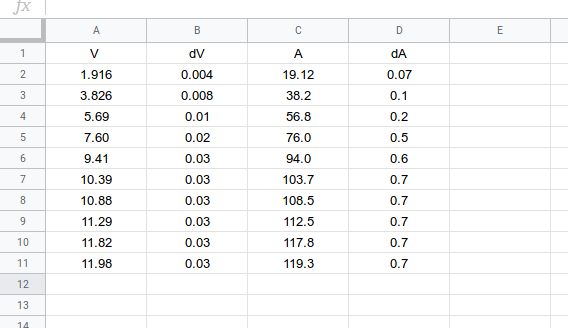
\includegraphics[width=0.7\textwidth]{basico/dados.png}

    \caption{Organização dos dados para importar em \python}
    \label{fig:basico:dados}
\end{figure}


\subsubsection{Arquivos CSV}

    Arquivos \texttt{CSV} (\textit{Comma Separated Values}) são os mais típicos para armazenamento de dados para análises. Eles são basicamente arquivos de textos, então podem ser visualizados e editados em qualquer editor de texto, mas os valores são separados por algum carácter específico, normalmente a vírgula (\texttt{,}), e as primeiras linhas podem ser utilizadas como \textit{header} dos dados.

    \begin{figure}[H]
        \centering
        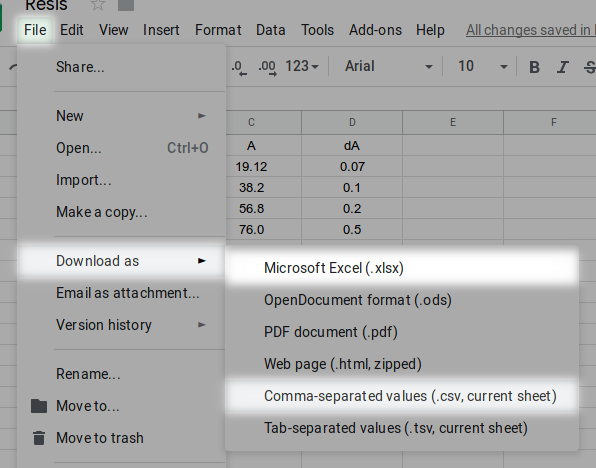
\includegraphics[width=0.6\textwidth]{basico/download.png}

        \caption{Recuperando os valores de uma folha de planilha no Google Planilhas}
        \label{fig:basico:download}
    \end{figure}

    Apesar de o exemplo da figura \ref{fig:basico:download} ser apenas no \texttt{Google Planilhas}, qualquer outro gerenciador de tabelas atual terá uma opção similar como parte do programa também. Uma vez que o \texttt{CSV} esteja pronto, ele pode ser transformado em um \dataframe com a função \pyref{http://pandas.pydata.org/pandas-docs/stable/reference/api/pandas.read_csv.html}{read\_csv} do \pandas.

    O argumento \pyline{decimal} da função representa qual o carácter a ser entendido como separador decimal. No exemplo do código \ref{code:basico:csv}, é usado a vírgula como separador, mas se por acaso estiver usando o ponto final para isso, lembre-se de mudar para \pyline{'.'}. Se o separador estiver diferente, o \pandas vai entender o valor como texto, o que não servirá para a montagem do gráfico depois.

    \begin{listing}[H]
        \caption{Leitura de um \dataframe a partir de um \texttt{CSV}}
        \label{code:basico:csv}

        \pyinclude[firstline=3,lastline=5]{recursos/basico/read.py}
    \end{listing}


\subsubsection{Arquivos do Excel}

    Também é possível ler diretamente arquivos do \texttt{Excel} ou arquivos do mesmo tipo (\texttt{.xlsx}) extraído de outro programa, como na figura \ref{fig:basico:download}. Para isso, além de expecificar o nome do arquivo, é necessário dizer qual a folha da planilha a ser usada com o argumento \pyline{sheet_name}, como no código \ref{code:basico:xlsx}, tudo com a função \pyref{http://pandas.pydata.org/pandas-docs/stable/reference/api/pandas.read_excel.html}{read\_excel}. Para este tipo de arquivo, não precisa preocupar com o separador de decimal, pois a representação interna do dado já é númerica, em vez de textual, como era no \texttt{CSV}.

    \begin{listing}[H]
        \caption{Leitura de um \dataframe a partir de um arquivo de \texttt{Excel}}
        \label{code:basico:xlsx}

        \pyinclude[firstline=7,lastline=9]{recursos/basico/read.py}
    \end{listing}


\subsection{Salvado os Gráficos}

    A interface \pyplot também ajuda na hora de salvar os gráficos em imagens, com a função \pyref{https://matplotlib.org/3.1.0/api/_as_gen/matplotlib.pyplot.savefig.html}{savefig}. Essa função reconhece o tipo do arquivo pela extensão e já vem com várias opções desde o início. Os tipos mais importantes normalmente são \texttt{PNG} e \texttt{PDF}, que podem ser criados seguindo os códigos \ref{code:basico:png} e  \ref{code:basico:pdf}. Para o \texttt{PNG}, também existe a opção de controlar a resolução pelo \texttt{DPI} da imagem, com o argumento \pyline{dpi}.

\begin{listing}[H]
    \caption{Salvando o gráfico em um arquivo \texttt{PNG}}
    \label{code:basico:png}

    \pyinclude[firstline=11, lastline=13]{recursos/basico/read.py}
\end{listing}

\begin{listing}[H]
    \caption{Salvando o gráfico em um arquivo \texttt{PDF}}
    \label{code:basico:pdf}

    \pyinclude[firstline=15, lastline=17]{recursos/basico/read.py}
\end{listing}

Para gráficos vetorizados, a opção mais usada é o \texttt{SVG}, que também é resolvido por padrão com o \matplotlib, fazendo como no código \ref{code:basico:svgpgf}. No entanto, quando se quer usar o gráfico em um documento de \LaTeX, uma opção muito útil é o \texttt{PGF}, que não passa de um arquivo de texto com comandos do pacote \texttt{pgf} para ser inserido em uma figura com um comando do tipo \mintinline{latex}{\input{grafico.pgf}}, mas cuidado com as configurações.

\begin{listing}[H]
    \caption{Salvando o gráfico em um arquivo \texttt{SVG} ou \texttt{PGF}}
    \label{code:basico:svgpgf}

    \pyinclude[firstline=19, lastline=23]{recursos/basico/read.py}
\end{listing}



    \section{Apresentação dos Dados} \label{sec:reta}
        \begin{table}[H]
    \centering
    \begin{tabular}{rr}
\toprule
  Tensão &   Corrente \\
\midrule
 -3.07 V &  -34.38 mA \\
 -2.70 V &  -27.96 mA \\
 -1.69 V &  -15.83 mA \\
 -1.47 V &  -10.79 mA \\
 -0.62 V &   -7.94 mA \\
 -0.04 V &   -0.05 mA \\
  0.72 V &    7.43 mA \\
  1.25 V &   13.37 mA \\
  2.35 V &   21.56 mA \\
  2.48 V &   31.34 mA \\
  3.38 V &   33.32 mA \\
\bottomrule
\end{tabular}

    \caption{Dados de corrente para cada tensão, gerados por computador}
    \label{tab:reta:dados}
\end{table}

Nesta seção, será tomado como exemplo a relação de corrente e tensão em um resistor, dado de forma teórica pela relação (\ref{eq:reta:corrente}). Por mais que os dados usados aqui sejam os da tabela \ref{tab:reta:dados}, essa parte de apresentação de dados é importante para todos os tipos de análise, em especial, para dados coletados manualmente, como é o caso da maioria dos experimentos da disciplina de \texttt{F 329}.

\begin{equacao} \label{eq:reta:corrente}
    I = \frac{1}{R} ~ V
\end{equacao}


\subsection{Dados Pontuais}

    \begin{listing}[H]
        \caption{Gerando um gráfico de dispersão}
        \label{code:reta:scatter}

        \pyinclude[firstline=11, lastline=15]{recursos/reta/reta.py}
    \end{listing}

    Para apresentar os dados coletados, a melhor opção é a função \pyref{https://matplotlib.org/3.1.0/api/_as_gen/matplotlib.pyplot.scatter.html}{scatter} do \pyplot, que recebe uma lista de valores de $x$ e outra lista de $y$ como argumentos e desenha cada ponto $(x, y)$.

    \begin{figure}[htbp]
        \centering
        %% Creator: Matplotlib, PGF backend
%%
%% To include the figure in your LaTeX document, write
%%   \input{<filename>.pgf}
%%
%% Make sure the required packages are loaded in your preamble
%%   \usepackage{pgf}
%%
%% Figures using additional raster images can only be included by \input if
%% they are in the same directory as the main LaTeX file. For loading figures
%% from other directories you can use the `import` package
%%   \usepackage{import}
%% and then include the figures with
%%   \import{<path to file>}{<filename>.pgf}
%%
%% Matplotlib used the following preamble
%%   
%%       \usepackage[portuguese]{babel}
%%       \usepackage[T1]{fontenc}
%%       \usepackage[utf8]{inputenc}
%%   \usepackage{fontspec}
%%
\begingroup%
\makeatletter%
\begin{pgfpicture}%
\pgfpathrectangle{\pgfpointorigin}{\pgfqpoint{4.500000in}{3.500000in}}%
\pgfusepath{use as bounding box, clip}%
\begin{pgfscope}%
\pgfsetbuttcap%
\pgfsetmiterjoin%
\pgfsetlinewidth{0.000000pt}%
\definecolor{currentstroke}{rgb}{0.000000,0.000000,0.000000}%
\pgfsetstrokecolor{currentstroke}%
\pgfsetstrokeopacity{0.000000}%
\pgfsetdash{}{0pt}%
\pgfpathmoveto{\pgfqpoint{0.000000in}{0.000000in}}%
\pgfpathlineto{\pgfqpoint{4.500000in}{0.000000in}}%
\pgfpathlineto{\pgfqpoint{4.500000in}{3.500000in}}%
\pgfpathlineto{\pgfqpoint{0.000000in}{3.500000in}}%
\pgfpathclose%
\pgfusepath{}%
\end{pgfscope}%
\begin{pgfscope}%
\pgfsetbuttcap%
\pgfsetmiterjoin%
\pgfsetlinewidth{0.000000pt}%
\definecolor{currentstroke}{rgb}{0.000000,0.000000,0.000000}%
\pgfsetstrokecolor{currentstroke}%
\pgfsetstrokeopacity{0.000000}%
\pgfsetdash{}{0pt}%
\pgfpathmoveto{\pgfqpoint{0.437657in}{0.330514in}}%
\pgfpathlineto{\pgfqpoint{4.350000in}{0.330514in}}%
\pgfpathlineto{\pgfqpoint{4.350000in}{3.350000in}}%
\pgfpathlineto{\pgfqpoint{0.437657in}{3.350000in}}%
\pgfpathclose%
\pgfusepath{}%
\end{pgfscope}%
\begin{pgfscope}%
\pgfpathrectangle{\pgfqpoint{0.437657in}{0.330514in}}{\pgfqpoint{3.912343in}{3.019486in}}%
\pgfusepath{clip}%
\pgfsetbuttcap%
\pgfsetroundjoin%
\pgfsetlinewidth{0.803000pt}%
\definecolor{currentstroke}{rgb}{0.800000,0.800000,0.800000}%
\pgfsetstrokecolor{currentstroke}%
\pgfsetdash{{2.960000pt}{1.280000pt}}{0.000000pt}%
\pgfpathmoveto{\pgfqpoint{0.658411in}{0.330514in}}%
\pgfpathlineto{\pgfqpoint{0.658411in}{3.350000in}}%
\pgfusepath{stroke}%
\end{pgfscope}%
\begin{pgfscope}%
\definecolor{textcolor}{rgb}{0.150000,0.150000,0.150000}%
\pgfsetstrokecolor{textcolor}%
\pgfsetfillcolor{textcolor}%
\pgftext[x=0.658411in,y=0.252737in,,top]{\color{textcolor}\rmfamily\fontsize{8.330000}{9.996000}\selectfont \(\displaystyle -3\)}%
\end{pgfscope}%
\begin{pgfscope}%
\pgfpathrectangle{\pgfqpoint{0.437657in}{0.330514in}}{\pgfqpoint{3.912343in}{3.019486in}}%
\pgfusepath{clip}%
\pgfsetbuttcap%
\pgfsetroundjoin%
\pgfsetlinewidth{0.803000pt}%
\definecolor{currentstroke}{rgb}{0.800000,0.800000,0.800000}%
\pgfsetstrokecolor{currentstroke}%
\pgfsetdash{{2.960000pt}{1.280000pt}}{0.000000pt}%
\pgfpathmoveto{\pgfqpoint{1.208464in}{0.330514in}}%
\pgfpathlineto{\pgfqpoint{1.208464in}{3.350000in}}%
\pgfusepath{stroke}%
\end{pgfscope}%
\begin{pgfscope}%
\definecolor{textcolor}{rgb}{0.150000,0.150000,0.150000}%
\pgfsetstrokecolor{textcolor}%
\pgfsetfillcolor{textcolor}%
\pgftext[x=1.208464in,y=0.252737in,,top]{\color{textcolor}\rmfamily\fontsize{8.330000}{9.996000}\selectfont \(\displaystyle -2\)}%
\end{pgfscope}%
\begin{pgfscope}%
\pgfpathrectangle{\pgfqpoint{0.437657in}{0.330514in}}{\pgfqpoint{3.912343in}{3.019486in}}%
\pgfusepath{clip}%
\pgfsetbuttcap%
\pgfsetroundjoin%
\pgfsetlinewidth{0.803000pt}%
\definecolor{currentstroke}{rgb}{0.800000,0.800000,0.800000}%
\pgfsetstrokecolor{currentstroke}%
\pgfsetdash{{2.960000pt}{1.280000pt}}{0.000000pt}%
\pgfpathmoveto{\pgfqpoint{1.758517in}{0.330514in}}%
\pgfpathlineto{\pgfqpoint{1.758517in}{3.350000in}}%
\pgfusepath{stroke}%
\end{pgfscope}%
\begin{pgfscope}%
\definecolor{textcolor}{rgb}{0.150000,0.150000,0.150000}%
\pgfsetstrokecolor{textcolor}%
\pgfsetfillcolor{textcolor}%
\pgftext[x=1.758517in,y=0.252737in,,top]{\color{textcolor}\rmfamily\fontsize{8.330000}{9.996000}\selectfont \(\displaystyle -1\)}%
\end{pgfscope}%
\begin{pgfscope}%
\pgfpathrectangle{\pgfqpoint{0.437657in}{0.330514in}}{\pgfqpoint{3.912343in}{3.019486in}}%
\pgfusepath{clip}%
\pgfsetbuttcap%
\pgfsetroundjoin%
\pgfsetlinewidth{0.803000pt}%
\definecolor{currentstroke}{rgb}{0.800000,0.800000,0.800000}%
\pgfsetstrokecolor{currentstroke}%
\pgfsetdash{{2.960000pt}{1.280000pt}}{0.000000pt}%
\pgfpathmoveto{\pgfqpoint{2.308570in}{0.330514in}}%
\pgfpathlineto{\pgfqpoint{2.308570in}{3.350000in}}%
\pgfusepath{stroke}%
\end{pgfscope}%
\begin{pgfscope}%
\definecolor{textcolor}{rgb}{0.150000,0.150000,0.150000}%
\pgfsetstrokecolor{textcolor}%
\pgfsetfillcolor{textcolor}%
\pgftext[x=2.308570in,y=0.252737in,,top]{\color{textcolor}\rmfamily\fontsize{8.330000}{9.996000}\selectfont \(\displaystyle 0\)}%
\end{pgfscope}%
\begin{pgfscope}%
\pgfpathrectangle{\pgfqpoint{0.437657in}{0.330514in}}{\pgfqpoint{3.912343in}{3.019486in}}%
\pgfusepath{clip}%
\pgfsetbuttcap%
\pgfsetroundjoin%
\pgfsetlinewidth{0.803000pt}%
\definecolor{currentstroke}{rgb}{0.800000,0.800000,0.800000}%
\pgfsetstrokecolor{currentstroke}%
\pgfsetdash{{2.960000pt}{1.280000pt}}{0.000000pt}%
\pgfpathmoveto{\pgfqpoint{2.858624in}{0.330514in}}%
\pgfpathlineto{\pgfqpoint{2.858624in}{3.350000in}}%
\pgfusepath{stroke}%
\end{pgfscope}%
\begin{pgfscope}%
\definecolor{textcolor}{rgb}{0.150000,0.150000,0.150000}%
\pgfsetstrokecolor{textcolor}%
\pgfsetfillcolor{textcolor}%
\pgftext[x=2.858624in,y=0.252737in,,top]{\color{textcolor}\rmfamily\fontsize{8.330000}{9.996000}\selectfont \(\displaystyle 1\)}%
\end{pgfscope}%
\begin{pgfscope}%
\pgfpathrectangle{\pgfqpoint{0.437657in}{0.330514in}}{\pgfqpoint{3.912343in}{3.019486in}}%
\pgfusepath{clip}%
\pgfsetbuttcap%
\pgfsetroundjoin%
\pgfsetlinewidth{0.803000pt}%
\definecolor{currentstroke}{rgb}{0.800000,0.800000,0.800000}%
\pgfsetstrokecolor{currentstroke}%
\pgfsetdash{{2.960000pt}{1.280000pt}}{0.000000pt}%
\pgfpathmoveto{\pgfqpoint{3.408677in}{0.330514in}}%
\pgfpathlineto{\pgfqpoint{3.408677in}{3.350000in}}%
\pgfusepath{stroke}%
\end{pgfscope}%
\begin{pgfscope}%
\definecolor{textcolor}{rgb}{0.150000,0.150000,0.150000}%
\pgfsetstrokecolor{textcolor}%
\pgfsetfillcolor{textcolor}%
\pgftext[x=3.408677in,y=0.252737in,,top]{\color{textcolor}\rmfamily\fontsize{8.330000}{9.996000}\selectfont \(\displaystyle 2\)}%
\end{pgfscope}%
\begin{pgfscope}%
\pgfpathrectangle{\pgfqpoint{0.437657in}{0.330514in}}{\pgfqpoint{3.912343in}{3.019486in}}%
\pgfusepath{clip}%
\pgfsetbuttcap%
\pgfsetroundjoin%
\pgfsetlinewidth{0.803000pt}%
\definecolor{currentstroke}{rgb}{0.800000,0.800000,0.800000}%
\pgfsetstrokecolor{currentstroke}%
\pgfsetdash{{2.960000pt}{1.280000pt}}{0.000000pt}%
\pgfpathmoveto{\pgfqpoint{3.958730in}{0.330514in}}%
\pgfpathlineto{\pgfqpoint{3.958730in}{3.350000in}}%
\pgfusepath{stroke}%
\end{pgfscope}%
\begin{pgfscope}%
\definecolor{textcolor}{rgb}{0.150000,0.150000,0.150000}%
\pgfsetstrokecolor{textcolor}%
\pgfsetfillcolor{textcolor}%
\pgftext[x=3.958730in,y=0.252737in,,top]{\color{textcolor}\rmfamily\fontsize{8.330000}{9.996000}\selectfont \(\displaystyle 3\)}%
\end{pgfscope}%
\begin{pgfscope}%
\pgfpathrectangle{\pgfqpoint{0.437657in}{0.330514in}}{\pgfqpoint{3.912343in}{3.019486in}}%
\pgfusepath{clip}%
\pgfsetbuttcap%
\pgfsetroundjoin%
\pgfsetlinewidth{0.803000pt}%
\definecolor{currentstroke}{rgb}{0.800000,0.800000,0.800000}%
\pgfsetstrokecolor{currentstroke}%
\pgfsetdash{{2.960000pt}{1.280000pt}}{0.000000pt}%
\pgfpathmoveto{\pgfqpoint{0.437657in}{0.645723in}}%
\pgfpathlineto{\pgfqpoint{4.350000in}{0.645723in}}%
\pgfusepath{stroke}%
\end{pgfscope}%
\begin{pgfscope}%
\definecolor{textcolor}{rgb}{0.150000,0.150000,0.150000}%
\pgfsetstrokecolor{textcolor}%
\pgfsetfillcolor{textcolor}%
\pgftext[x=0.150000in,y=0.605577in,left,base]{\color{textcolor}\rmfamily\fontsize{8.330000}{9.996000}\selectfont \(\displaystyle -30\)}%
\end{pgfscope}%
\begin{pgfscope}%
\pgfpathrectangle{\pgfqpoint{0.437657in}{0.330514in}}{\pgfqpoint{3.912343in}{3.019486in}}%
\pgfusepath{clip}%
\pgfsetbuttcap%
\pgfsetroundjoin%
\pgfsetlinewidth{0.803000pt}%
\definecolor{currentstroke}{rgb}{0.800000,0.800000,0.800000}%
\pgfsetstrokecolor{currentstroke}%
\pgfsetdash{{2.960000pt}{1.280000pt}}{0.000000pt}%
\pgfpathmoveto{\pgfqpoint{0.437657in}{1.051062in}}%
\pgfpathlineto{\pgfqpoint{4.350000in}{1.051062in}}%
\pgfusepath{stroke}%
\end{pgfscope}%
\begin{pgfscope}%
\definecolor{textcolor}{rgb}{0.150000,0.150000,0.150000}%
\pgfsetstrokecolor{textcolor}%
\pgfsetfillcolor{textcolor}%
\pgftext[x=0.150000in,y=1.010916in,left,base]{\color{textcolor}\rmfamily\fontsize{8.330000}{9.996000}\selectfont \(\displaystyle -20\)}%
\end{pgfscope}%
\begin{pgfscope}%
\pgfpathrectangle{\pgfqpoint{0.437657in}{0.330514in}}{\pgfqpoint{3.912343in}{3.019486in}}%
\pgfusepath{clip}%
\pgfsetbuttcap%
\pgfsetroundjoin%
\pgfsetlinewidth{0.803000pt}%
\definecolor{currentstroke}{rgb}{0.800000,0.800000,0.800000}%
\pgfsetstrokecolor{currentstroke}%
\pgfsetdash{{2.960000pt}{1.280000pt}}{0.000000pt}%
\pgfpathmoveto{\pgfqpoint{0.437657in}{1.456401in}}%
\pgfpathlineto{\pgfqpoint{4.350000in}{1.456401in}}%
\pgfusepath{stroke}%
\end{pgfscope}%
\begin{pgfscope}%
\definecolor{textcolor}{rgb}{0.150000,0.150000,0.150000}%
\pgfsetstrokecolor{textcolor}%
\pgfsetfillcolor{textcolor}%
\pgftext[x=0.150000in,y=1.416255in,left,base]{\color{textcolor}\rmfamily\fontsize{8.330000}{9.996000}\selectfont \(\displaystyle -10\)}%
\end{pgfscope}%
\begin{pgfscope}%
\pgfpathrectangle{\pgfqpoint{0.437657in}{0.330514in}}{\pgfqpoint{3.912343in}{3.019486in}}%
\pgfusepath{clip}%
\pgfsetbuttcap%
\pgfsetroundjoin%
\pgfsetlinewidth{0.803000pt}%
\definecolor{currentstroke}{rgb}{0.800000,0.800000,0.800000}%
\pgfsetstrokecolor{currentstroke}%
\pgfsetdash{{2.960000pt}{1.280000pt}}{0.000000pt}%
\pgfpathmoveto{\pgfqpoint{0.437657in}{1.861740in}}%
\pgfpathlineto{\pgfqpoint{4.350000in}{1.861740in}}%
\pgfusepath{stroke}%
\end{pgfscope}%
\begin{pgfscope}%
\definecolor{textcolor}{rgb}{0.150000,0.150000,0.150000}%
\pgfsetstrokecolor{textcolor}%
\pgfsetfillcolor{textcolor}%
\pgftext[x=0.300851in,y=1.821594in,left,base]{\color{textcolor}\rmfamily\fontsize{8.330000}{9.996000}\selectfont \(\displaystyle 0\)}%
\end{pgfscope}%
\begin{pgfscope}%
\pgfpathrectangle{\pgfqpoint{0.437657in}{0.330514in}}{\pgfqpoint{3.912343in}{3.019486in}}%
\pgfusepath{clip}%
\pgfsetbuttcap%
\pgfsetroundjoin%
\pgfsetlinewidth{0.803000pt}%
\definecolor{currentstroke}{rgb}{0.800000,0.800000,0.800000}%
\pgfsetstrokecolor{currentstroke}%
\pgfsetdash{{2.960000pt}{1.280000pt}}{0.000000pt}%
\pgfpathmoveto{\pgfqpoint{0.437657in}{2.267079in}}%
\pgfpathlineto{\pgfqpoint{4.350000in}{2.267079in}}%
\pgfusepath{stroke}%
\end{pgfscope}%
\begin{pgfscope}%
\definecolor{textcolor}{rgb}{0.150000,0.150000,0.150000}%
\pgfsetstrokecolor{textcolor}%
\pgfsetfillcolor{textcolor}%
\pgftext[x=0.241822in,y=2.226933in,left,base]{\color{textcolor}\rmfamily\fontsize{8.330000}{9.996000}\selectfont \(\displaystyle 10\)}%
\end{pgfscope}%
\begin{pgfscope}%
\pgfpathrectangle{\pgfqpoint{0.437657in}{0.330514in}}{\pgfqpoint{3.912343in}{3.019486in}}%
\pgfusepath{clip}%
\pgfsetbuttcap%
\pgfsetroundjoin%
\pgfsetlinewidth{0.803000pt}%
\definecolor{currentstroke}{rgb}{0.800000,0.800000,0.800000}%
\pgfsetstrokecolor{currentstroke}%
\pgfsetdash{{2.960000pt}{1.280000pt}}{0.000000pt}%
\pgfpathmoveto{\pgfqpoint{0.437657in}{2.672418in}}%
\pgfpathlineto{\pgfqpoint{4.350000in}{2.672418in}}%
\pgfusepath{stroke}%
\end{pgfscope}%
\begin{pgfscope}%
\definecolor{textcolor}{rgb}{0.150000,0.150000,0.150000}%
\pgfsetstrokecolor{textcolor}%
\pgfsetfillcolor{textcolor}%
\pgftext[x=0.241822in,y=2.632272in,left,base]{\color{textcolor}\rmfamily\fontsize{8.330000}{9.996000}\selectfont \(\displaystyle 20\)}%
\end{pgfscope}%
\begin{pgfscope}%
\pgfpathrectangle{\pgfqpoint{0.437657in}{0.330514in}}{\pgfqpoint{3.912343in}{3.019486in}}%
\pgfusepath{clip}%
\pgfsetbuttcap%
\pgfsetroundjoin%
\pgfsetlinewidth{0.803000pt}%
\definecolor{currentstroke}{rgb}{0.800000,0.800000,0.800000}%
\pgfsetstrokecolor{currentstroke}%
\pgfsetdash{{2.960000pt}{1.280000pt}}{0.000000pt}%
\pgfpathmoveto{\pgfqpoint{0.437657in}{3.077757in}}%
\pgfpathlineto{\pgfqpoint{4.350000in}{3.077757in}}%
\pgfusepath{stroke}%
\end{pgfscope}%
\begin{pgfscope}%
\definecolor{textcolor}{rgb}{0.150000,0.150000,0.150000}%
\pgfsetstrokecolor{textcolor}%
\pgfsetfillcolor{textcolor}%
\pgftext[x=0.241822in,y=3.037611in,left,base]{\color{textcolor}\rmfamily\fontsize{8.330000}{9.996000}\selectfont \(\displaystyle 30\)}%
\end{pgfscope}%
\begin{pgfscope}%
\pgfpathrectangle{\pgfqpoint{0.437657in}{0.330514in}}{\pgfqpoint{3.912343in}{3.019486in}}%
\pgfusepath{clip}%
\pgfsetbuttcap%
\pgfsetroundjoin%
\definecolor{currentfill}{rgb}{0.282353,0.470588,0.811765}%
\pgfsetfillcolor{currentfill}%
\pgfsetlinewidth{0.240900pt}%
\definecolor{currentstroke}{rgb}{0.282353,0.470588,0.811765}%
\pgfsetstrokecolor{currentstroke}%
\pgfsetdash{}{0pt}%
\pgfpathmoveto{\pgfqpoint{0.619907in}{0.429296in}}%
\pgfpathcurveto{\pgfqpoint{0.630221in}{0.429296in}}{\pgfqpoint{0.640113in}{0.433393in}}{\pgfqpoint{0.647406in}{0.440686in}}%
\pgfpathcurveto{\pgfqpoint{0.654699in}{0.447979in}}{\pgfqpoint{0.658796in}{0.457871in}}{\pgfqpoint{0.658796in}{0.468185in}}%
\pgfpathcurveto{\pgfqpoint{0.658796in}{0.478498in}}{\pgfqpoint{0.654699in}{0.488391in}}{\pgfqpoint{0.647406in}{0.495683in}}%
\pgfpathcurveto{\pgfqpoint{0.640113in}{0.502976in}}{\pgfqpoint{0.630221in}{0.507074in}}{\pgfqpoint{0.619907in}{0.507074in}}%
\pgfpathcurveto{\pgfqpoint{0.609594in}{0.507074in}}{\pgfqpoint{0.599701in}{0.502976in}}{\pgfqpoint{0.592409in}{0.495683in}}%
\pgfpathcurveto{\pgfqpoint{0.585116in}{0.488391in}}{\pgfqpoint{0.581018in}{0.478498in}}{\pgfqpoint{0.581018in}{0.468185in}}%
\pgfpathcurveto{\pgfqpoint{0.581018in}{0.457871in}}{\pgfqpoint{0.585116in}{0.447979in}}{\pgfqpoint{0.592409in}{0.440686in}}%
\pgfpathcurveto{\pgfqpoint{0.599701in}{0.433393in}}{\pgfqpoint{0.609594in}{0.429296in}}{\pgfqpoint{0.619907in}{0.429296in}}%
\pgfpathclose%
\pgfusepath{stroke,fill}%
\end{pgfscope}%
\begin{pgfscope}%
\pgfpathrectangle{\pgfqpoint{0.437657in}{0.330514in}}{\pgfqpoint{3.912343in}{3.019486in}}%
\pgfusepath{clip}%
\pgfsetbuttcap%
\pgfsetroundjoin%
\definecolor{currentfill}{rgb}{0.282353,0.470588,0.811765}%
\pgfsetfillcolor{currentfill}%
\pgfsetlinewidth{0.240900pt}%
\definecolor{currentstroke}{rgb}{0.282353,0.470588,0.811765}%
\pgfsetstrokecolor{currentstroke}%
\pgfsetdash{}{0pt}%
\pgfpathmoveto{\pgfqpoint{0.823427in}{0.689524in}}%
\pgfpathcurveto{\pgfqpoint{0.833740in}{0.689524in}}{\pgfqpoint{0.843633in}{0.693621in}}{\pgfqpoint{0.850926in}{0.700914in}}%
\pgfpathcurveto{\pgfqpoint{0.858218in}{0.708207in}}{\pgfqpoint{0.862316in}{0.718099in}}{\pgfqpoint{0.862316in}{0.728412in}}%
\pgfpathcurveto{\pgfqpoint{0.862316in}{0.738726in}}{\pgfqpoint{0.858218in}{0.748618in}}{\pgfqpoint{0.850926in}{0.755911in}}%
\pgfpathcurveto{\pgfqpoint{0.843633in}{0.763204in}}{\pgfqpoint{0.833740in}{0.767301in}}{\pgfqpoint{0.823427in}{0.767301in}}%
\pgfpathcurveto{\pgfqpoint{0.813114in}{0.767301in}}{\pgfqpoint{0.803221in}{0.763204in}}{\pgfqpoint{0.795928in}{0.755911in}}%
\pgfpathcurveto{\pgfqpoint{0.788636in}{0.748618in}}{\pgfqpoint{0.784538in}{0.738726in}}{\pgfqpoint{0.784538in}{0.728412in}}%
\pgfpathcurveto{\pgfqpoint{0.784538in}{0.718099in}}{\pgfqpoint{0.788636in}{0.708207in}}{\pgfqpoint{0.795928in}{0.700914in}}%
\pgfpathcurveto{\pgfqpoint{0.803221in}{0.693621in}}{\pgfqpoint{0.813114in}{0.689524in}}{\pgfqpoint{0.823427in}{0.689524in}}%
\pgfpathclose%
\pgfusepath{stroke,fill}%
\end{pgfscope}%
\begin{pgfscope}%
\pgfpathrectangle{\pgfqpoint{0.437657in}{0.330514in}}{\pgfqpoint{3.912343in}{3.019486in}}%
\pgfusepath{clip}%
\pgfsetbuttcap%
\pgfsetroundjoin%
\definecolor{currentfill}{rgb}{0.282353,0.470588,0.811765}%
\pgfsetfillcolor{currentfill}%
\pgfsetlinewidth{0.240900pt}%
\definecolor{currentstroke}{rgb}{0.282353,0.470588,0.811765}%
\pgfsetstrokecolor{currentstroke}%
\pgfsetdash{}{0pt}%
\pgfpathmoveto{\pgfqpoint{1.378981in}{1.181200in}}%
\pgfpathcurveto{\pgfqpoint{1.389294in}{1.181200in}}{\pgfqpoint{1.399187in}{1.185297in}}{\pgfqpoint{1.406479in}{1.192590in}}%
\pgfpathcurveto{\pgfqpoint{1.413772in}{1.199883in}}{\pgfqpoint{1.417870in}{1.209775in}}{\pgfqpoint{1.417870in}{1.220089in}}%
\pgfpathcurveto{\pgfqpoint{1.417870in}{1.230402in}}{\pgfqpoint{1.413772in}{1.240294in}}{\pgfqpoint{1.406479in}{1.247587in}}%
\pgfpathcurveto{\pgfqpoint{1.399187in}{1.254880in}}{\pgfqpoint{1.389294in}{1.258977in}}{\pgfqpoint{1.378981in}{1.258977in}}%
\pgfpathcurveto{\pgfqpoint{1.368667in}{1.258977in}}{\pgfqpoint{1.358775in}{1.254880in}}{\pgfqpoint{1.351482in}{1.247587in}}%
\pgfpathcurveto{\pgfqpoint{1.344189in}{1.240294in}}{\pgfqpoint{1.340092in}{1.230402in}}{\pgfqpoint{1.340092in}{1.220089in}}%
\pgfpathcurveto{\pgfqpoint{1.340092in}{1.209775in}}{\pgfqpoint{1.344189in}{1.199883in}}{\pgfqpoint{1.351482in}{1.192590in}}%
\pgfpathcurveto{\pgfqpoint{1.358775in}{1.185297in}}{\pgfqpoint{1.368667in}{1.181200in}}{\pgfqpoint{1.378981in}{1.181200in}}%
\pgfpathclose%
\pgfusepath{stroke,fill}%
\end{pgfscope}%
\begin{pgfscope}%
\pgfpathrectangle{\pgfqpoint{0.437657in}{0.330514in}}{\pgfqpoint{3.912343in}{3.019486in}}%
\pgfusepath{clip}%
\pgfsetbuttcap%
\pgfsetroundjoin%
\definecolor{currentfill}{rgb}{0.282353,0.470588,0.811765}%
\pgfsetfillcolor{currentfill}%
\pgfsetlinewidth{0.240900pt}%
\definecolor{currentstroke}{rgb}{0.282353,0.470588,0.811765}%
\pgfsetstrokecolor{currentstroke}%
\pgfsetdash{}{0pt}%
\pgfpathmoveto{\pgfqpoint{1.499992in}{1.385490in}}%
\pgfpathcurveto{\pgfqpoint{1.510306in}{1.385490in}}{\pgfqpoint{1.520198in}{1.389588in}}{\pgfqpoint{1.527491in}{1.396881in}}%
\pgfpathcurveto{\pgfqpoint{1.534784in}{1.404174in}}{\pgfqpoint{1.538881in}{1.414066in}}{\pgfqpoint{1.538881in}{1.424379in}}%
\pgfpathcurveto{\pgfqpoint{1.538881in}{1.434693in}}{\pgfqpoint{1.534784in}{1.444585in}}{\pgfqpoint{1.527491in}{1.451878in}}%
\pgfpathcurveto{\pgfqpoint{1.520198in}{1.459171in}}{\pgfqpoint{1.510306in}{1.463268in}}{\pgfqpoint{1.499992in}{1.463268in}}%
\pgfpathcurveto{\pgfqpoint{1.489679in}{1.463268in}}{\pgfqpoint{1.479786in}{1.459171in}}{\pgfqpoint{1.472494in}{1.451878in}}%
\pgfpathcurveto{\pgfqpoint{1.465201in}{1.444585in}}{\pgfqpoint{1.461103in}{1.434693in}}{\pgfqpoint{1.461103in}{1.424379in}}%
\pgfpathcurveto{\pgfqpoint{1.461103in}{1.414066in}}{\pgfqpoint{1.465201in}{1.404174in}}{\pgfqpoint{1.472494in}{1.396881in}}%
\pgfpathcurveto{\pgfqpoint{1.479786in}{1.389588in}}{\pgfqpoint{1.489679in}{1.385490in}}{\pgfqpoint{1.499992in}{1.385490in}}%
\pgfpathclose%
\pgfusepath{stroke,fill}%
\end{pgfscope}%
\begin{pgfscope}%
\pgfpathrectangle{\pgfqpoint{0.437657in}{0.330514in}}{\pgfqpoint{3.912343in}{3.019486in}}%
\pgfusepath{clip}%
\pgfsetbuttcap%
\pgfsetroundjoin%
\definecolor{currentfill}{rgb}{0.282353,0.470588,0.811765}%
\pgfsetfillcolor{currentfill}%
\pgfsetlinewidth{0.240900pt}%
\definecolor{currentstroke}{rgb}{0.282353,0.470588,0.811765}%
\pgfsetstrokecolor{currentstroke}%
\pgfsetdash{}{0pt}%
\pgfpathmoveto{\pgfqpoint{1.967537in}{1.501012in}}%
\pgfpathcurveto{\pgfqpoint{1.977851in}{1.501012in}}{\pgfqpoint{1.987743in}{1.505110in}}{\pgfqpoint{1.995036in}{1.512402in}}%
\pgfpathcurveto{\pgfqpoint{2.002329in}{1.519695in}}{\pgfqpoint{2.006426in}{1.529588in}}{\pgfqpoint{2.006426in}{1.539901in}}%
\pgfpathcurveto{\pgfqpoint{2.006426in}{1.550214in}}{\pgfqpoint{2.002329in}{1.560107in}}{\pgfqpoint{1.995036in}{1.567400in}}%
\pgfpathcurveto{\pgfqpoint{1.987743in}{1.574692in}}{\pgfqpoint{1.977851in}{1.578790in}}{\pgfqpoint{1.967537in}{1.578790in}}%
\pgfpathcurveto{\pgfqpoint{1.957224in}{1.578790in}}{\pgfqpoint{1.947332in}{1.574692in}}{\pgfqpoint{1.940039in}{1.567400in}}%
\pgfpathcurveto{\pgfqpoint{1.932746in}{1.560107in}}{\pgfqpoint{1.928649in}{1.550214in}}{\pgfqpoint{1.928649in}{1.539901in}}%
\pgfpathcurveto{\pgfqpoint{1.928649in}{1.529588in}}{\pgfqpoint{1.932746in}{1.519695in}}{\pgfqpoint{1.940039in}{1.512402in}}%
\pgfpathcurveto{\pgfqpoint{1.947332in}{1.505110in}}{\pgfqpoint{1.957224in}{1.501012in}}{\pgfqpoint{1.967537in}{1.501012in}}%
\pgfpathclose%
\pgfusepath{stroke,fill}%
\end{pgfscope}%
\begin{pgfscope}%
\pgfpathrectangle{\pgfqpoint{0.437657in}{0.330514in}}{\pgfqpoint{3.912343in}{3.019486in}}%
\pgfusepath{clip}%
\pgfsetbuttcap%
\pgfsetroundjoin%
\definecolor{currentfill}{rgb}{0.282353,0.470588,0.811765}%
\pgfsetfillcolor{currentfill}%
\pgfsetlinewidth{0.240900pt}%
\definecolor{currentstroke}{rgb}{0.282353,0.470588,0.811765}%
\pgfsetstrokecolor{currentstroke}%
\pgfsetdash{}{0pt}%
\pgfpathmoveto{\pgfqpoint{2.286568in}{1.820825in}}%
\pgfpathcurveto{\pgfqpoint{2.296882in}{1.820825in}}{\pgfqpoint{2.306774in}{1.824922in}}{\pgfqpoint{2.314067in}{1.832215in}}%
\pgfpathcurveto{\pgfqpoint{2.321360in}{1.839508in}}{\pgfqpoint{2.325457in}{1.849400in}}{\pgfqpoint{2.325457in}{1.859713in}}%
\pgfpathcurveto{\pgfqpoint{2.325457in}{1.870027in}}{\pgfqpoint{2.321360in}{1.879919in}}{\pgfqpoint{2.314067in}{1.887212in}}%
\pgfpathcurveto{\pgfqpoint{2.306774in}{1.894505in}}{\pgfqpoint{2.296882in}{1.898602in}}{\pgfqpoint{2.286568in}{1.898602in}}%
\pgfpathcurveto{\pgfqpoint{2.276255in}{1.898602in}}{\pgfqpoint{2.266362in}{1.894505in}}{\pgfqpoint{2.259070in}{1.887212in}}%
\pgfpathcurveto{\pgfqpoint{2.251777in}{1.879919in}}{\pgfqpoint{2.247679in}{1.870027in}}{\pgfqpoint{2.247679in}{1.859713in}}%
\pgfpathcurveto{\pgfqpoint{2.247679in}{1.849400in}}{\pgfqpoint{2.251777in}{1.839508in}}{\pgfqpoint{2.259070in}{1.832215in}}%
\pgfpathcurveto{\pgfqpoint{2.266362in}{1.824922in}}{\pgfqpoint{2.276255in}{1.820825in}}{\pgfqpoint{2.286568in}{1.820825in}}%
\pgfpathclose%
\pgfusepath{stroke,fill}%
\end{pgfscope}%
\begin{pgfscope}%
\pgfpathrectangle{\pgfqpoint{0.437657in}{0.330514in}}{\pgfqpoint{3.912343in}{3.019486in}}%
\pgfusepath{clip}%
\pgfsetbuttcap%
\pgfsetroundjoin%
\definecolor{currentfill}{rgb}{0.282353,0.470588,0.811765}%
\pgfsetfillcolor{currentfill}%
\pgfsetlinewidth{0.240900pt}%
\definecolor{currentstroke}{rgb}{0.282353,0.470588,0.811765}%
\pgfsetstrokecolor{currentstroke}%
\pgfsetdash{}{0pt}%
\pgfpathmoveto{\pgfqpoint{2.704609in}{2.124018in}}%
\pgfpathcurveto{\pgfqpoint{2.714922in}{2.124018in}}{\pgfqpoint{2.724815in}{2.128116in}}{\pgfqpoint{2.732107in}{2.135408in}}%
\pgfpathcurveto{\pgfqpoint{2.739400in}{2.142701in}}{\pgfqpoint{2.743498in}{2.152594in}}{\pgfqpoint{2.743498in}{2.162907in}}%
\pgfpathcurveto{\pgfqpoint{2.743498in}{2.173220in}}{\pgfqpoint{2.739400in}{2.183113in}}{\pgfqpoint{2.732107in}{2.190406in}}%
\pgfpathcurveto{\pgfqpoint{2.724815in}{2.197698in}}{\pgfqpoint{2.714922in}{2.201796in}}{\pgfqpoint{2.704609in}{2.201796in}}%
\pgfpathcurveto{\pgfqpoint{2.694295in}{2.201796in}}{\pgfqpoint{2.684403in}{2.197698in}}{\pgfqpoint{2.677110in}{2.190406in}}%
\pgfpathcurveto{\pgfqpoint{2.669817in}{2.183113in}}{\pgfqpoint{2.665720in}{2.173220in}}{\pgfqpoint{2.665720in}{2.162907in}}%
\pgfpathcurveto{\pgfqpoint{2.665720in}{2.152594in}}{\pgfqpoint{2.669817in}{2.142701in}}{\pgfqpoint{2.677110in}{2.135408in}}%
\pgfpathcurveto{\pgfqpoint{2.684403in}{2.128116in}}{\pgfqpoint{2.694295in}{2.124018in}}{\pgfqpoint{2.704609in}{2.124018in}}%
\pgfpathclose%
\pgfusepath{stroke,fill}%
\end{pgfscope}%
\begin{pgfscope}%
\pgfpathrectangle{\pgfqpoint{0.437657in}{0.330514in}}{\pgfqpoint{3.912343in}{3.019486in}}%
\pgfusepath{clip}%
\pgfsetbuttcap%
\pgfsetroundjoin%
\definecolor{currentfill}{rgb}{0.282353,0.470588,0.811765}%
\pgfsetfillcolor{currentfill}%
\pgfsetlinewidth{0.240900pt}%
\definecolor{currentstroke}{rgb}{0.282353,0.470588,0.811765}%
\pgfsetstrokecolor{currentstroke}%
\pgfsetdash{}{0pt}%
\pgfpathmoveto{\pgfqpoint{2.996137in}{2.364789in}}%
\pgfpathcurveto{\pgfqpoint{3.006450in}{2.364789in}}{\pgfqpoint{3.016343in}{2.368887in}}{\pgfqpoint{3.023635in}{2.376180in}}%
\pgfpathcurveto{\pgfqpoint{3.030928in}{2.383472in}}{\pgfqpoint{3.035026in}{2.393365in}}{\pgfqpoint{3.035026in}{2.403678in}}%
\pgfpathcurveto{\pgfqpoint{3.035026in}{2.413992in}}{\pgfqpoint{3.030928in}{2.423884in}}{\pgfqpoint{3.023635in}{2.431177in}}%
\pgfpathcurveto{\pgfqpoint{3.016343in}{2.438470in}}{\pgfqpoint{3.006450in}{2.442567in}}{\pgfqpoint{2.996137in}{2.442567in}}%
\pgfpathcurveto{\pgfqpoint{2.985823in}{2.442567in}}{\pgfqpoint{2.975931in}{2.438470in}}{\pgfqpoint{2.968638in}{2.431177in}}%
\pgfpathcurveto{\pgfqpoint{2.961346in}{2.423884in}}{\pgfqpoint{2.957248in}{2.413992in}}{\pgfqpoint{2.957248in}{2.403678in}}%
\pgfpathcurveto{\pgfqpoint{2.957248in}{2.393365in}}{\pgfqpoint{2.961346in}{2.383472in}}{\pgfqpoint{2.968638in}{2.376180in}}%
\pgfpathcurveto{\pgfqpoint{2.975931in}{2.368887in}}{\pgfqpoint{2.985823in}{2.364789in}}{\pgfqpoint{2.996137in}{2.364789in}}%
\pgfpathclose%
\pgfusepath{stroke,fill}%
\end{pgfscope}%
\begin{pgfscope}%
\pgfpathrectangle{\pgfqpoint{0.437657in}{0.330514in}}{\pgfqpoint{3.912343in}{3.019486in}}%
\pgfusepath{clip}%
\pgfsetbuttcap%
\pgfsetroundjoin%
\definecolor{currentfill}{rgb}{0.282353,0.470588,0.811765}%
\pgfsetfillcolor{currentfill}%
\pgfsetlinewidth{0.240900pt}%
\definecolor{currentstroke}{rgb}{0.282353,0.470588,0.811765}%
\pgfsetstrokecolor{currentstroke}%
\pgfsetdash{}{0pt}%
\pgfpathmoveto{\pgfqpoint{3.601195in}{2.696762in}}%
\pgfpathcurveto{\pgfqpoint{3.611509in}{2.696762in}}{\pgfqpoint{3.621401in}{2.700860in}}{\pgfqpoint{3.628694in}{2.708152in}}%
\pgfpathcurveto{\pgfqpoint{3.635987in}{2.715445in}}{\pgfqpoint{3.640084in}{2.725337in}}{\pgfqpoint{3.640084in}{2.735651in}}%
\pgfpathcurveto{\pgfqpoint{3.640084in}{2.745964in}}{\pgfqpoint{3.635987in}{2.755857in}}{\pgfqpoint{3.628694in}{2.763150in}}%
\pgfpathcurveto{\pgfqpoint{3.621401in}{2.770442in}}{\pgfqpoint{3.611509in}{2.774540in}}{\pgfqpoint{3.601195in}{2.774540in}}%
\pgfpathcurveto{\pgfqpoint{3.590882in}{2.774540in}}{\pgfqpoint{3.580989in}{2.770442in}}{\pgfqpoint{3.573697in}{2.763150in}}%
\pgfpathcurveto{\pgfqpoint{3.566404in}{2.755857in}}{\pgfqpoint{3.562306in}{2.745964in}}{\pgfqpoint{3.562306in}{2.735651in}}%
\pgfpathcurveto{\pgfqpoint{3.562306in}{2.725337in}}{\pgfqpoint{3.566404in}{2.715445in}}{\pgfqpoint{3.573697in}{2.708152in}}%
\pgfpathcurveto{\pgfqpoint{3.580989in}{2.700860in}}{\pgfqpoint{3.590882in}{2.696762in}}{\pgfqpoint{3.601195in}{2.696762in}}%
\pgfpathclose%
\pgfusepath{stroke,fill}%
\end{pgfscope}%
\begin{pgfscope}%
\pgfpathrectangle{\pgfqpoint{0.437657in}{0.330514in}}{\pgfqpoint{3.912343in}{3.019486in}}%
\pgfusepath{clip}%
\pgfsetbuttcap%
\pgfsetroundjoin%
\definecolor{currentfill}{rgb}{0.282353,0.470588,0.811765}%
\pgfsetfillcolor{currentfill}%
\pgfsetlinewidth{0.240900pt}%
\definecolor{currentstroke}{rgb}{0.282353,0.470588,0.811765}%
\pgfsetstrokecolor{currentstroke}%
\pgfsetdash{}{0pt}%
\pgfpathmoveto{\pgfqpoint{3.672702in}{3.093184in}}%
\pgfpathcurveto{\pgfqpoint{3.683016in}{3.093184in}}{\pgfqpoint{3.692908in}{3.097281in}}{\pgfqpoint{3.700201in}{3.104574in}}%
\pgfpathcurveto{\pgfqpoint{3.707494in}{3.111867in}}{\pgfqpoint{3.711591in}{3.121759in}}{\pgfqpoint{3.711591in}{3.132072in}}%
\pgfpathcurveto{\pgfqpoint{3.711591in}{3.142386in}}{\pgfqpoint{3.707494in}{3.152278in}}{\pgfqpoint{3.700201in}{3.159571in}}%
\pgfpathcurveto{\pgfqpoint{3.692908in}{3.166864in}}{\pgfqpoint{3.683016in}{3.170961in}}{\pgfqpoint{3.672702in}{3.170961in}}%
\pgfpathcurveto{\pgfqpoint{3.662389in}{3.170961in}}{\pgfqpoint{3.652496in}{3.166864in}}{\pgfqpoint{3.645204in}{3.159571in}}%
\pgfpathcurveto{\pgfqpoint{3.637911in}{3.152278in}}{\pgfqpoint{3.633813in}{3.142386in}}{\pgfqpoint{3.633813in}{3.132072in}}%
\pgfpathcurveto{\pgfqpoint{3.633813in}{3.121759in}}{\pgfqpoint{3.637911in}{3.111867in}}{\pgfqpoint{3.645204in}{3.104574in}}%
\pgfpathcurveto{\pgfqpoint{3.652496in}{3.097281in}}{\pgfqpoint{3.662389in}{3.093184in}}{\pgfqpoint{3.672702in}{3.093184in}}%
\pgfpathclose%
\pgfusepath{stroke,fill}%
\end{pgfscope}%
\begin{pgfscope}%
\pgfpathrectangle{\pgfqpoint{0.437657in}{0.330514in}}{\pgfqpoint{3.912343in}{3.019486in}}%
\pgfusepath{clip}%
\pgfsetbuttcap%
\pgfsetroundjoin%
\definecolor{currentfill}{rgb}{0.282353,0.470588,0.811765}%
\pgfsetfillcolor{currentfill}%
\pgfsetlinewidth{0.240900pt}%
\definecolor{currentstroke}{rgb}{0.282353,0.470588,0.811765}%
\pgfsetstrokecolor{currentstroke}%
\pgfsetdash{}{0pt}%
\pgfpathmoveto{\pgfqpoint{4.167750in}{3.173441in}}%
\pgfpathcurveto{\pgfqpoint{4.178064in}{3.173441in}}{\pgfqpoint{4.187956in}{3.177538in}}{\pgfqpoint{4.195249in}{3.184831in}}%
\pgfpathcurveto{\pgfqpoint{4.202541in}{3.192124in}}{\pgfqpoint{4.206639in}{3.202016in}}{\pgfqpoint{4.206639in}{3.212330in}}%
\pgfpathcurveto{\pgfqpoint{4.206639in}{3.222643in}}{\pgfqpoint{4.202541in}{3.232535in}}{\pgfqpoint{4.195249in}{3.239828in}}%
\pgfpathcurveto{\pgfqpoint{4.187956in}{3.247121in}}{\pgfqpoint{4.178064in}{3.251218in}}{\pgfqpoint{4.167750in}{3.251218in}}%
\pgfpathcurveto{\pgfqpoint{4.157437in}{3.251218in}}{\pgfqpoint{4.147544in}{3.247121in}}{\pgfqpoint{4.140251in}{3.239828in}}%
\pgfpathcurveto{\pgfqpoint{4.132959in}{3.232535in}}{\pgfqpoint{4.128861in}{3.222643in}}{\pgfqpoint{4.128861in}{3.212330in}}%
\pgfpathcurveto{\pgfqpoint{4.128861in}{3.202016in}}{\pgfqpoint{4.132959in}{3.192124in}}{\pgfqpoint{4.140251in}{3.184831in}}%
\pgfpathcurveto{\pgfqpoint{4.147544in}{3.177538in}}{\pgfqpoint{4.157437in}{3.173441in}}{\pgfqpoint{4.167750in}{3.173441in}}%
\pgfpathclose%
\pgfusepath{stroke,fill}%
\end{pgfscope}%
\begin{pgfscope}%
\pgfsetrectcap%
\pgfsetmiterjoin%
\pgfsetlinewidth{1.003750pt}%
\definecolor{currentstroke}{rgb}{0.400000,0.400000,0.400000}%
\pgfsetstrokecolor{currentstroke}%
\pgfsetdash{}{0pt}%
\pgfpathmoveto{\pgfqpoint{0.437657in}{0.330514in}}%
\pgfpathlineto{\pgfqpoint{0.437657in}{3.350000in}}%
\pgfusepath{stroke}%
\end{pgfscope}%
\begin{pgfscope}%
\pgfsetrectcap%
\pgfsetmiterjoin%
\pgfsetlinewidth{1.003750pt}%
\definecolor{currentstroke}{rgb}{0.400000,0.400000,0.400000}%
\pgfsetstrokecolor{currentstroke}%
\pgfsetdash{}{0pt}%
\pgfpathmoveto{\pgfqpoint{0.437657in}{0.330514in}}%
\pgfpathlineto{\pgfqpoint{4.350000in}{0.330514in}}%
\pgfusepath{stroke}%
\end{pgfscope}%
\end{pgfpicture}%
\makeatother%
\endgroup%


        \caption{Gráfico de dispersão dos pontos}
        \label{fig:reta:dados}
    \end{figure}


\subsection{Texto dos Eixos e do Título}

    Em um gŕafico como este, é necessário colocar texto no título e nos rótulos (\textit{label}) dos eixos.

    \begin{listing}[H]
        \caption{Montagem dos textos do gráfico}
        \label{code:reta:textos}

        \pyinclude[firstline=19, lastline=25]{recursos/reta/reta.py}
    \end{listing}


\subsection{Resultado}

    \begin{figure}[htbp]
        \centering
        %% Creator: Matplotlib, PGF backend
%%
%% To include the figure in your LaTeX document, write
%%   \input{<filename>.pgf}
%%
%% Make sure the required packages are loaded in your preamble
%%   \usepackage{pgf}
%%
%% Figures using additional raster images can only be included by \input if
%% they are in the same directory as the main LaTeX file. For loading figures
%% from other directories you can use the `import` package
%%   \usepackage{import}
%% and then include the figures with
%%   \import{<path to file>}{<filename>.pgf}
%%
%% Matplotlib used the following preamble
%%   
%%       \usepackage[portuguese]{babel}
%%       \usepackage[T1]{fontenc}
%%       \usepackage[utf8]{inputenc}
%%   \usepackage{fontspec}
%%
\begingroup%
\makeatletter%
\begin{pgfpicture}%
\pgfpathrectangle{\pgfpointorigin}{\pgfqpoint{4.500000in}{3.500000in}}%
\pgfusepath{use as bounding box, clip}%
\begin{pgfscope}%
\pgfsetbuttcap%
\pgfsetmiterjoin%
\definecolor{currentfill}{rgb}{1.000000,1.000000,1.000000}%
\pgfsetfillcolor{currentfill}%
\pgfsetlinewidth{0.000000pt}%
\definecolor{currentstroke}{rgb}{1.000000,1.000000,1.000000}%
\pgfsetstrokecolor{currentstroke}%
\pgfsetdash{}{0pt}%
\pgfpathmoveto{\pgfqpoint{0.000000in}{0.000000in}}%
\pgfpathlineto{\pgfqpoint{4.500000in}{0.000000in}}%
\pgfpathlineto{\pgfqpoint{4.500000in}{3.500000in}}%
\pgfpathlineto{\pgfqpoint{0.000000in}{3.500000in}}%
\pgfpathclose%
\pgfusepath{fill}%
\end{pgfscope}%
\begin{pgfscope}%
\pgfsetbuttcap%
\pgfsetmiterjoin%
\definecolor{currentfill}{rgb}{1.000000,1.000000,1.000000}%
\pgfsetfillcolor{currentfill}%
\pgfsetlinewidth{0.000000pt}%
\definecolor{currentstroke}{rgb}{0.000000,0.000000,0.000000}%
\pgfsetstrokecolor{currentstroke}%
\pgfsetstrokeopacity{0.000000}%
\pgfsetdash{}{0pt}%
\pgfpathmoveto{\pgfqpoint{0.632102in}{0.524958in}}%
\pgfpathlineto{\pgfqpoint{4.350000in}{0.524958in}}%
\pgfpathlineto{\pgfqpoint{4.350000in}{3.149333in}}%
\pgfpathlineto{\pgfqpoint{0.632102in}{3.149333in}}%
\pgfpathclose%
\pgfusepath{fill}%
\end{pgfscope}%
\begin{pgfscope}%
\pgfpathrectangle{\pgfqpoint{0.632102in}{0.524958in}}{\pgfqpoint{3.717898in}{2.624375in}}%
\pgfusepath{clip}%
\pgfsetbuttcap%
\pgfsetroundjoin%
\pgfsetlinewidth{0.803000pt}%
\definecolor{currentstroke}{rgb}{0.800000,0.800000,0.800000}%
\pgfsetstrokecolor{currentstroke}%
\pgfsetdash{{2.960000pt}{1.280000pt}}{0.000000pt}%
\pgfpathmoveto{\pgfqpoint{0.841884in}{0.524958in}}%
\pgfpathlineto{\pgfqpoint{0.841884in}{3.149333in}}%
\pgfusepath{stroke}%
\end{pgfscope}%
\begin{pgfscope}%
\definecolor{textcolor}{rgb}{0.150000,0.150000,0.150000}%
\pgfsetstrokecolor{textcolor}%
\pgfsetfillcolor{textcolor}%
\pgftext[x=0.841884in,y=0.447181in,,top]{\color{textcolor}\rmfamily\fontsize{8.330000}{9.996000}\selectfont \(\displaystyle -3\)}%
\end{pgfscope}%
\begin{pgfscope}%
\pgfpathrectangle{\pgfqpoint{0.632102in}{0.524958in}}{\pgfqpoint{3.717898in}{2.624375in}}%
\pgfusepath{clip}%
\pgfsetbuttcap%
\pgfsetroundjoin%
\pgfsetlinewidth{0.803000pt}%
\definecolor{currentstroke}{rgb}{0.800000,0.800000,0.800000}%
\pgfsetstrokecolor{currentstroke}%
\pgfsetdash{{2.960000pt}{1.280000pt}}{0.000000pt}%
\pgfpathmoveto{\pgfqpoint{1.364599in}{0.524958in}}%
\pgfpathlineto{\pgfqpoint{1.364599in}{3.149333in}}%
\pgfusepath{stroke}%
\end{pgfscope}%
\begin{pgfscope}%
\definecolor{textcolor}{rgb}{0.150000,0.150000,0.150000}%
\pgfsetstrokecolor{textcolor}%
\pgfsetfillcolor{textcolor}%
\pgftext[x=1.364599in,y=0.447181in,,top]{\color{textcolor}\rmfamily\fontsize{8.330000}{9.996000}\selectfont \(\displaystyle -2\)}%
\end{pgfscope}%
\begin{pgfscope}%
\pgfpathrectangle{\pgfqpoint{0.632102in}{0.524958in}}{\pgfqpoint{3.717898in}{2.624375in}}%
\pgfusepath{clip}%
\pgfsetbuttcap%
\pgfsetroundjoin%
\pgfsetlinewidth{0.803000pt}%
\definecolor{currentstroke}{rgb}{0.800000,0.800000,0.800000}%
\pgfsetstrokecolor{currentstroke}%
\pgfsetdash{{2.960000pt}{1.280000pt}}{0.000000pt}%
\pgfpathmoveto{\pgfqpoint{1.887314in}{0.524958in}}%
\pgfpathlineto{\pgfqpoint{1.887314in}{3.149333in}}%
\pgfusepath{stroke}%
\end{pgfscope}%
\begin{pgfscope}%
\definecolor{textcolor}{rgb}{0.150000,0.150000,0.150000}%
\pgfsetstrokecolor{textcolor}%
\pgfsetfillcolor{textcolor}%
\pgftext[x=1.887314in,y=0.447181in,,top]{\color{textcolor}\rmfamily\fontsize{8.330000}{9.996000}\selectfont \(\displaystyle -1\)}%
\end{pgfscope}%
\begin{pgfscope}%
\pgfpathrectangle{\pgfqpoint{0.632102in}{0.524958in}}{\pgfqpoint{3.717898in}{2.624375in}}%
\pgfusepath{clip}%
\pgfsetbuttcap%
\pgfsetroundjoin%
\pgfsetlinewidth{0.803000pt}%
\definecolor{currentstroke}{rgb}{0.800000,0.800000,0.800000}%
\pgfsetstrokecolor{currentstroke}%
\pgfsetdash{{2.960000pt}{1.280000pt}}{0.000000pt}%
\pgfpathmoveto{\pgfqpoint{2.410030in}{0.524958in}}%
\pgfpathlineto{\pgfqpoint{2.410030in}{3.149333in}}%
\pgfusepath{stroke}%
\end{pgfscope}%
\begin{pgfscope}%
\definecolor{textcolor}{rgb}{0.150000,0.150000,0.150000}%
\pgfsetstrokecolor{textcolor}%
\pgfsetfillcolor{textcolor}%
\pgftext[x=2.410030in,y=0.447181in,,top]{\color{textcolor}\rmfamily\fontsize{8.330000}{9.996000}\selectfont \(\displaystyle 0\)}%
\end{pgfscope}%
\begin{pgfscope}%
\pgfpathrectangle{\pgfqpoint{0.632102in}{0.524958in}}{\pgfqpoint{3.717898in}{2.624375in}}%
\pgfusepath{clip}%
\pgfsetbuttcap%
\pgfsetroundjoin%
\pgfsetlinewidth{0.803000pt}%
\definecolor{currentstroke}{rgb}{0.800000,0.800000,0.800000}%
\pgfsetstrokecolor{currentstroke}%
\pgfsetdash{{2.960000pt}{1.280000pt}}{0.000000pt}%
\pgfpathmoveto{\pgfqpoint{2.932745in}{0.524958in}}%
\pgfpathlineto{\pgfqpoint{2.932745in}{3.149333in}}%
\pgfusepath{stroke}%
\end{pgfscope}%
\begin{pgfscope}%
\definecolor{textcolor}{rgb}{0.150000,0.150000,0.150000}%
\pgfsetstrokecolor{textcolor}%
\pgfsetfillcolor{textcolor}%
\pgftext[x=2.932745in,y=0.447181in,,top]{\color{textcolor}\rmfamily\fontsize{8.330000}{9.996000}\selectfont \(\displaystyle 1\)}%
\end{pgfscope}%
\begin{pgfscope}%
\pgfpathrectangle{\pgfqpoint{0.632102in}{0.524958in}}{\pgfqpoint{3.717898in}{2.624375in}}%
\pgfusepath{clip}%
\pgfsetbuttcap%
\pgfsetroundjoin%
\pgfsetlinewidth{0.803000pt}%
\definecolor{currentstroke}{rgb}{0.800000,0.800000,0.800000}%
\pgfsetstrokecolor{currentstroke}%
\pgfsetdash{{2.960000pt}{1.280000pt}}{0.000000pt}%
\pgfpathmoveto{\pgfqpoint{3.455461in}{0.524958in}}%
\pgfpathlineto{\pgfqpoint{3.455461in}{3.149333in}}%
\pgfusepath{stroke}%
\end{pgfscope}%
\begin{pgfscope}%
\definecolor{textcolor}{rgb}{0.150000,0.150000,0.150000}%
\pgfsetstrokecolor{textcolor}%
\pgfsetfillcolor{textcolor}%
\pgftext[x=3.455461in,y=0.447181in,,top]{\color{textcolor}\rmfamily\fontsize{8.330000}{9.996000}\selectfont \(\displaystyle 2\)}%
\end{pgfscope}%
\begin{pgfscope}%
\pgfpathrectangle{\pgfqpoint{0.632102in}{0.524958in}}{\pgfqpoint{3.717898in}{2.624375in}}%
\pgfusepath{clip}%
\pgfsetbuttcap%
\pgfsetroundjoin%
\pgfsetlinewidth{0.803000pt}%
\definecolor{currentstroke}{rgb}{0.800000,0.800000,0.800000}%
\pgfsetstrokecolor{currentstroke}%
\pgfsetdash{{2.960000pt}{1.280000pt}}{0.000000pt}%
\pgfpathmoveto{\pgfqpoint{3.978176in}{0.524958in}}%
\pgfpathlineto{\pgfqpoint{3.978176in}{3.149333in}}%
\pgfusepath{stroke}%
\end{pgfscope}%
\begin{pgfscope}%
\definecolor{textcolor}{rgb}{0.150000,0.150000,0.150000}%
\pgfsetstrokecolor{textcolor}%
\pgfsetfillcolor{textcolor}%
\pgftext[x=3.978176in,y=0.447181in,,top]{\color{textcolor}\rmfamily\fontsize{8.330000}{9.996000}\selectfont \(\displaystyle 3\)}%
\end{pgfscope}%
\begin{pgfscope}%
\definecolor{textcolor}{rgb}{0.000000,0.000000,0.000000}%
\pgfsetstrokecolor{textcolor}%
\pgfsetfillcolor{textcolor}%
\pgftext[x=2.491051in,y=0.288889in,,top]{\color{textcolor}\rmfamily\fontsize{10.000000}{12.000000}\selectfont Tensão [V]}%
\end{pgfscope}%
\begin{pgfscope}%
\pgfpathrectangle{\pgfqpoint{0.632102in}{0.524958in}}{\pgfqpoint{3.717898in}{2.624375in}}%
\pgfusepath{clip}%
\pgfsetbuttcap%
\pgfsetroundjoin%
\pgfsetlinewidth{0.803000pt}%
\definecolor{currentstroke}{rgb}{0.800000,0.800000,0.800000}%
\pgfsetstrokecolor{currentstroke}%
\pgfsetdash{{2.960000pt}{1.280000pt}}{0.000000pt}%
\pgfpathmoveto{\pgfqpoint{0.632102in}{0.798921in}}%
\pgfpathlineto{\pgfqpoint{4.350000in}{0.798921in}}%
\pgfusepath{stroke}%
\end{pgfscope}%
\begin{pgfscope}%
\definecolor{textcolor}{rgb}{0.150000,0.150000,0.150000}%
\pgfsetstrokecolor{textcolor}%
\pgfsetfillcolor{textcolor}%
\pgftext[x=0.344444in,y=0.758775in,left,base]{\color{textcolor}\rmfamily\fontsize{8.330000}{9.996000}\selectfont \(\displaystyle -30\)}%
\end{pgfscope}%
\begin{pgfscope}%
\pgfpathrectangle{\pgfqpoint{0.632102in}{0.524958in}}{\pgfqpoint{3.717898in}{2.624375in}}%
\pgfusepath{clip}%
\pgfsetbuttcap%
\pgfsetroundjoin%
\pgfsetlinewidth{0.803000pt}%
\definecolor{currentstroke}{rgb}{0.800000,0.800000,0.800000}%
\pgfsetstrokecolor{currentstroke}%
\pgfsetdash{{2.960000pt}{1.280000pt}}{0.000000pt}%
\pgfpathmoveto{\pgfqpoint{0.632102in}{1.151220in}}%
\pgfpathlineto{\pgfqpoint{4.350000in}{1.151220in}}%
\pgfusepath{stroke}%
\end{pgfscope}%
\begin{pgfscope}%
\definecolor{textcolor}{rgb}{0.150000,0.150000,0.150000}%
\pgfsetstrokecolor{textcolor}%
\pgfsetfillcolor{textcolor}%
\pgftext[x=0.344444in,y=1.111074in,left,base]{\color{textcolor}\rmfamily\fontsize{8.330000}{9.996000}\selectfont \(\displaystyle -20\)}%
\end{pgfscope}%
\begin{pgfscope}%
\pgfpathrectangle{\pgfqpoint{0.632102in}{0.524958in}}{\pgfqpoint{3.717898in}{2.624375in}}%
\pgfusepath{clip}%
\pgfsetbuttcap%
\pgfsetroundjoin%
\pgfsetlinewidth{0.803000pt}%
\definecolor{currentstroke}{rgb}{0.800000,0.800000,0.800000}%
\pgfsetstrokecolor{currentstroke}%
\pgfsetdash{{2.960000pt}{1.280000pt}}{0.000000pt}%
\pgfpathmoveto{\pgfqpoint{0.632102in}{1.503519in}}%
\pgfpathlineto{\pgfqpoint{4.350000in}{1.503519in}}%
\pgfusepath{stroke}%
\end{pgfscope}%
\begin{pgfscope}%
\definecolor{textcolor}{rgb}{0.150000,0.150000,0.150000}%
\pgfsetstrokecolor{textcolor}%
\pgfsetfillcolor{textcolor}%
\pgftext[x=0.344444in,y=1.463373in,left,base]{\color{textcolor}\rmfamily\fontsize{8.330000}{9.996000}\selectfont \(\displaystyle -10\)}%
\end{pgfscope}%
\begin{pgfscope}%
\pgfpathrectangle{\pgfqpoint{0.632102in}{0.524958in}}{\pgfqpoint{3.717898in}{2.624375in}}%
\pgfusepath{clip}%
\pgfsetbuttcap%
\pgfsetroundjoin%
\pgfsetlinewidth{0.803000pt}%
\definecolor{currentstroke}{rgb}{0.800000,0.800000,0.800000}%
\pgfsetstrokecolor{currentstroke}%
\pgfsetdash{{2.960000pt}{1.280000pt}}{0.000000pt}%
\pgfpathmoveto{\pgfqpoint{0.632102in}{1.855818in}}%
\pgfpathlineto{\pgfqpoint{4.350000in}{1.855818in}}%
\pgfusepath{stroke}%
\end{pgfscope}%
\begin{pgfscope}%
\definecolor{textcolor}{rgb}{0.150000,0.150000,0.150000}%
\pgfsetstrokecolor{textcolor}%
\pgfsetfillcolor{textcolor}%
\pgftext[x=0.495295in,y=1.815672in,left,base]{\color{textcolor}\rmfamily\fontsize{8.330000}{9.996000}\selectfont \(\displaystyle 0\)}%
\end{pgfscope}%
\begin{pgfscope}%
\pgfpathrectangle{\pgfqpoint{0.632102in}{0.524958in}}{\pgfqpoint{3.717898in}{2.624375in}}%
\pgfusepath{clip}%
\pgfsetbuttcap%
\pgfsetroundjoin%
\pgfsetlinewidth{0.803000pt}%
\definecolor{currentstroke}{rgb}{0.800000,0.800000,0.800000}%
\pgfsetstrokecolor{currentstroke}%
\pgfsetdash{{2.960000pt}{1.280000pt}}{0.000000pt}%
\pgfpathmoveto{\pgfqpoint{0.632102in}{2.208117in}}%
\pgfpathlineto{\pgfqpoint{4.350000in}{2.208117in}}%
\pgfusepath{stroke}%
\end{pgfscope}%
\begin{pgfscope}%
\definecolor{textcolor}{rgb}{0.150000,0.150000,0.150000}%
\pgfsetstrokecolor{textcolor}%
\pgfsetfillcolor{textcolor}%
\pgftext[x=0.436267in,y=2.167971in,left,base]{\color{textcolor}\rmfamily\fontsize{8.330000}{9.996000}\selectfont \(\displaystyle 10\)}%
\end{pgfscope}%
\begin{pgfscope}%
\pgfpathrectangle{\pgfqpoint{0.632102in}{0.524958in}}{\pgfqpoint{3.717898in}{2.624375in}}%
\pgfusepath{clip}%
\pgfsetbuttcap%
\pgfsetroundjoin%
\pgfsetlinewidth{0.803000pt}%
\definecolor{currentstroke}{rgb}{0.800000,0.800000,0.800000}%
\pgfsetstrokecolor{currentstroke}%
\pgfsetdash{{2.960000pt}{1.280000pt}}{0.000000pt}%
\pgfpathmoveto{\pgfqpoint{0.632102in}{2.560415in}}%
\pgfpathlineto{\pgfqpoint{4.350000in}{2.560415in}}%
\pgfusepath{stroke}%
\end{pgfscope}%
\begin{pgfscope}%
\definecolor{textcolor}{rgb}{0.150000,0.150000,0.150000}%
\pgfsetstrokecolor{textcolor}%
\pgfsetfillcolor{textcolor}%
\pgftext[x=0.436267in,y=2.520269in,left,base]{\color{textcolor}\rmfamily\fontsize{8.330000}{9.996000}\selectfont \(\displaystyle 20\)}%
\end{pgfscope}%
\begin{pgfscope}%
\pgfpathrectangle{\pgfqpoint{0.632102in}{0.524958in}}{\pgfqpoint{3.717898in}{2.624375in}}%
\pgfusepath{clip}%
\pgfsetbuttcap%
\pgfsetroundjoin%
\pgfsetlinewidth{0.803000pt}%
\definecolor{currentstroke}{rgb}{0.800000,0.800000,0.800000}%
\pgfsetstrokecolor{currentstroke}%
\pgfsetdash{{2.960000pt}{1.280000pt}}{0.000000pt}%
\pgfpathmoveto{\pgfqpoint{0.632102in}{2.912714in}}%
\pgfpathlineto{\pgfqpoint{4.350000in}{2.912714in}}%
\pgfusepath{stroke}%
\end{pgfscope}%
\begin{pgfscope}%
\definecolor{textcolor}{rgb}{0.150000,0.150000,0.150000}%
\pgfsetstrokecolor{textcolor}%
\pgfsetfillcolor{textcolor}%
\pgftext[x=0.436267in,y=2.872568in,left,base]{\color{textcolor}\rmfamily\fontsize{8.330000}{9.996000}\selectfont \(\displaystyle 30\)}%
\end{pgfscope}%
\begin{pgfscope}%
\definecolor{textcolor}{rgb}{0.000000,0.000000,0.000000}%
\pgfsetstrokecolor{textcolor}%
\pgfsetfillcolor{textcolor}%
\pgftext[x=0.288889in,y=1.837146in,,bottom,rotate=90.000000]{\color{textcolor}\rmfamily\fontsize{10.000000}{12.000000}\selectfont Corrente [mA]}%
\end{pgfscope}%
\begin{pgfscope}%
\pgfpathrectangle{\pgfqpoint{0.632102in}{0.524958in}}{\pgfqpoint{3.717898in}{2.624375in}}%
\pgfusepath{clip}%
\pgfsetbuttcap%
\pgfsetroundjoin%
\definecolor{currentfill}{rgb}{0.282353,0.470588,0.811765}%
\pgfsetfillcolor{currentfill}%
\pgfsetlinewidth{0.240900pt}%
\definecolor{currentstroke}{rgb}{0.282353,0.470588,0.811765}%
\pgfsetstrokecolor{currentstroke}%
\pgfsetdash{}{0pt}%
\pgfpathmoveto{\pgfqpoint{0.805294in}{0.605725in}}%
\pgfpathcurveto{\pgfqpoint{0.815607in}{0.605725in}}{\pgfqpoint{0.825500in}{0.609823in}}{\pgfqpoint{0.832792in}{0.617116in}}%
\pgfpathcurveto{\pgfqpoint{0.840085in}{0.624408in}}{\pgfqpoint{0.844183in}{0.634301in}}{\pgfqpoint{0.844183in}{0.644614in}}%
\pgfpathcurveto{\pgfqpoint{0.844183in}{0.654928in}}{\pgfqpoint{0.840085in}{0.664820in}}{\pgfqpoint{0.832792in}{0.672113in}}%
\pgfpathcurveto{\pgfqpoint{0.825500in}{0.679406in}}{\pgfqpoint{0.815607in}{0.683503in}}{\pgfqpoint{0.805294in}{0.683503in}}%
\pgfpathcurveto{\pgfqpoint{0.794980in}{0.683503in}}{\pgfqpoint{0.785088in}{0.679406in}}{\pgfqpoint{0.777795in}{0.672113in}}%
\pgfpathcurveto{\pgfqpoint{0.770502in}{0.664820in}}{\pgfqpoint{0.766405in}{0.654928in}}{\pgfqpoint{0.766405in}{0.644614in}}%
\pgfpathcurveto{\pgfqpoint{0.766405in}{0.634301in}}{\pgfqpoint{0.770502in}{0.624408in}}{\pgfqpoint{0.777795in}{0.617116in}}%
\pgfpathcurveto{\pgfqpoint{0.785088in}{0.609823in}}{\pgfqpoint{0.794980in}{0.605725in}}{\pgfqpoint{0.805294in}{0.605725in}}%
\pgfpathclose%
\pgfusepath{stroke,fill}%
\end{pgfscope}%
\begin{pgfscope}%
\pgfpathrectangle{\pgfqpoint{0.632102in}{0.524958in}}{\pgfqpoint{3.717898in}{2.624375in}}%
\pgfusepath{clip}%
\pgfsetbuttcap%
\pgfsetroundjoin%
\definecolor{currentfill}{rgb}{0.282353,0.470588,0.811765}%
\pgfsetfillcolor{currentfill}%
\pgfsetlinewidth{0.240900pt}%
\definecolor{currentstroke}{rgb}{0.282353,0.470588,0.811765}%
\pgfsetstrokecolor{currentstroke}%
\pgfsetdash{}{0pt}%
\pgfpathmoveto{\pgfqpoint{0.998698in}{0.831901in}}%
\pgfpathcurveto{\pgfqpoint{1.009012in}{0.831901in}}{\pgfqpoint{1.018904in}{0.835999in}}{\pgfqpoint{1.026197in}{0.843292in}}%
\pgfpathcurveto{\pgfqpoint{1.033490in}{0.850584in}}{\pgfqpoint{1.037587in}{0.860477in}}{\pgfqpoint{1.037587in}{0.870790in}}%
\pgfpathcurveto{\pgfqpoint{1.037587in}{0.881104in}}{\pgfqpoint{1.033490in}{0.890996in}}{\pgfqpoint{1.026197in}{0.898289in}}%
\pgfpathcurveto{\pgfqpoint{1.018904in}{0.905581in}}{\pgfqpoint{1.009012in}{0.909679in}}{\pgfqpoint{0.998698in}{0.909679in}}%
\pgfpathcurveto{\pgfqpoint{0.988385in}{0.909679in}}{\pgfqpoint{0.978492in}{0.905581in}}{\pgfqpoint{0.971200in}{0.898289in}}%
\pgfpathcurveto{\pgfqpoint{0.963907in}{0.890996in}}{\pgfqpoint{0.959809in}{0.881104in}}{\pgfqpoint{0.959809in}{0.870790in}}%
\pgfpathcurveto{\pgfqpoint{0.959809in}{0.860477in}}{\pgfqpoint{0.963907in}{0.850584in}}{\pgfqpoint{0.971200in}{0.843292in}}%
\pgfpathcurveto{\pgfqpoint{0.978492in}{0.835999in}}{\pgfqpoint{0.988385in}{0.831901in}}{\pgfqpoint{0.998698in}{0.831901in}}%
\pgfpathclose%
\pgfusepath{stroke,fill}%
\end{pgfscope}%
\begin{pgfscope}%
\pgfpathrectangle{\pgfqpoint{0.632102in}{0.524958in}}{\pgfqpoint{3.717898in}{2.624375in}}%
\pgfusepath{clip}%
\pgfsetbuttcap%
\pgfsetroundjoin%
\definecolor{currentfill}{rgb}{0.282353,0.470588,0.811765}%
\pgfsetfillcolor{currentfill}%
\pgfsetlinewidth{0.240900pt}%
\definecolor{currentstroke}{rgb}{0.282353,0.470588,0.811765}%
\pgfsetstrokecolor{currentstroke}%
\pgfsetdash{}{0pt}%
\pgfpathmoveto{\pgfqpoint{1.526641in}{1.259240in}}%
\pgfpathcurveto{\pgfqpoint{1.536954in}{1.259240in}}{\pgfqpoint{1.546847in}{1.263337in}}{\pgfqpoint{1.554139in}{1.270630in}}%
\pgfpathcurveto{\pgfqpoint{1.561432in}{1.277923in}}{\pgfqpoint{1.565530in}{1.287815in}}{\pgfqpoint{1.565530in}{1.298129in}}%
\pgfpathcurveto{\pgfqpoint{1.565530in}{1.308442in}}{\pgfqpoint{1.561432in}{1.318335in}}{\pgfqpoint{1.554139in}{1.325627in}}%
\pgfpathcurveto{\pgfqpoint{1.546847in}{1.332920in}}{\pgfqpoint{1.536954in}{1.337018in}}{\pgfqpoint{1.526641in}{1.337018in}}%
\pgfpathcurveto{\pgfqpoint{1.516327in}{1.337018in}}{\pgfqpoint{1.506435in}{1.332920in}}{\pgfqpoint{1.499142in}{1.325627in}}%
\pgfpathcurveto{\pgfqpoint{1.491850in}{1.318335in}}{\pgfqpoint{1.487752in}{1.308442in}}{\pgfqpoint{1.487752in}{1.298129in}}%
\pgfpathcurveto{\pgfqpoint{1.487752in}{1.287815in}}{\pgfqpoint{1.491850in}{1.277923in}}{\pgfqpoint{1.499142in}{1.270630in}}%
\pgfpathcurveto{\pgfqpoint{1.506435in}{1.263337in}}{\pgfqpoint{1.516327in}{1.259240in}}{\pgfqpoint{1.526641in}{1.259240in}}%
\pgfpathclose%
\pgfusepath{stroke,fill}%
\end{pgfscope}%
\begin{pgfscope}%
\pgfpathrectangle{\pgfqpoint{0.632102in}{0.524958in}}{\pgfqpoint{3.717898in}{2.624375in}}%
\pgfusepath{clip}%
\pgfsetbuttcap%
\pgfsetroundjoin%
\definecolor{currentfill}{rgb}{0.282353,0.470588,0.811765}%
\pgfsetfillcolor{currentfill}%
\pgfsetlinewidth{0.240900pt}%
\definecolor{currentstroke}{rgb}{0.282353,0.470588,0.811765}%
\pgfsetstrokecolor{currentstroke}%
\pgfsetdash{}{0pt}%
\pgfpathmoveto{\pgfqpoint{1.641638in}{1.436798in}}%
\pgfpathcurveto{\pgfqpoint{1.651952in}{1.436798in}}{\pgfqpoint{1.661844in}{1.440896in}}{\pgfqpoint{1.669137in}{1.448189in}}%
\pgfpathcurveto{\pgfqpoint{1.676430in}{1.455481in}}{\pgfqpoint{1.680527in}{1.465374in}}{\pgfqpoint{1.680527in}{1.475687in}}%
\pgfpathcurveto{\pgfqpoint{1.680527in}{1.486001in}}{\pgfqpoint{1.676430in}{1.495893in}}{\pgfqpoint{1.669137in}{1.503186in}}%
\pgfpathcurveto{\pgfqpoint{1.661844in}{1.510479in}}{\pgfqpoint{1.651952in}{1.514576in}}{\pgfqpoint{1.641638in}{1.514576in}}%
\pgfpathcurveto{\pgfqpoint{1.631325in}{1.514576in}}{\pgfqpoint{1.621432in}{1.510479in}}{\pgfqpoint{1.614140in}{1.503186in}}%
\pgfpathcurveto{\pgfqpoint{1.606847in}{1.495893in}}{\pgfqpoint{1.602749in}{1.486001in}}{\pgfqpoint{1.602749in}{1.475687in}}%
\pgfpathcurveto{\pgfqpoint{1.602749in}{1.465374in}}{\pgfqpoint{1.606847in}{1.455481in}}{\pgfqpoint{1.614140in}{1.448189in}}%
\pgfpathcurveto{\pgfqpoint{1.621432in}{1.440896in}}{\pgfqpoint{1.631325in}{1.436798in}}{\pgfqpoint{1.641638in}{1.436798in}}%
\pgfpathclose%
\pgfusepath{stroke,fill}%
\end{pgfscope}%
\begin{pgfscope}%
\pgfpathrectangle{\pgfqpoint{0.632102in}{0.524958in}}{\pgfqpoint{3.717898in}{2.624375in}}%
\pgfusepath{clip}%
\pgfsetbuttcap%
\pgfsetroundjoin%
\definecolor{currentfill}{rgb}{0.282353,0.470588,0.811765}%
\pgfsetfillcolor{currentfill}%
\pgfsetlinewidth{0.240900pt}%
\definecolor{currentstroke}{rgb}{0.282353,0.470588,0.811765}%
\pgfsetstrokecolor{currentstroke}%
\pgfsetdash{}{0pt}%
\pgfpathmoveto{\pgfqpoint{2.085946in}{1.537204in}}%
\pgfpathcurveto{\pgfqpoint{2.096260in}{1.537204in}}{\pgfqpoint{2.106152in}{1.541301in}}{\pgfqpoint{2.113445in}{1.548594in}}%
\pgfpathcurveto{\pgfqpoint{2.120738in}{1.555887in}}{\pgfqpoint{2.124835in}{1.565779in}}{\pgfqpoint{2.124835in}{1.576092in}}%
\pgfpathcurveto{\pgfqpoint{2.124835in}{1.586406in}}{\pgfqpoint{2.120738in}{1.596298in}}{\pgfqpoint{2.113445in}{1.603591in}}%
\pgfpathcurveto{\pgfqpoint{2.106152in}{1.610884in}}{\pgfqpoint{2.096260in}{1.614981in}}{\pgfqpoint{2.085946in}{1.614981in}}%
\pgfpathcurveto{\pgfqpoint{2.075633in}{1.614981in}}{\pgfqpoint{2.065740in}{1.610884in}}{\pgfqpoint{2.058448in}{1.603591in}}%
\pgfpathcurveto{\pgfqpoint{2.051155in}{1.596298in}}{\pgfqpoint{2.047057in}{1.586406in}}{\pgfqpoint{2.047057in}{1.576092in}}%
\pgfpathcurveto{\pgfqpoint{2.047057in}{1.565779in}}{\pgfqpoint{2.051155in}{1.555887in}}{\pgfqpoint{2.058448in}{1.548594in}}%
\pgfpathcurveto{\pgfqpoint{2.065740in}{1.541301in}}{\pgfqpoint{2.075633in}{1.537204in}}{\pgfqpoint{2.085946in}{1.537204in}}%
\pgfpathclose%
\pgfusepath{stroke,fill}%
\end{pgfscope}%
\begin{pgfscope}%
\pgfpathrectangle{\pgfqpoint{0.632102in}{0.524958in}}{\pgfqpoint{3.717898in}{2.624375in}}%
\pgfusepath{clip}%
\pgfsetbuttcap%
\pgfsetroundjoin%
\definecolor{currentfill}{rgb}{0.282353,0.470588,0.811765}%
\pgfsetfillcolor{currentfill}%
\pgfsetlinewidth{0.240900pt}%
\definecolor{currentstroke}{rgb}{0.282353,0.470588,0.811765}%
\pgfsetstrokecolor{currentstroke}%
\pgfsetdash{}{0pt}%
\pgfpathmoveto{\pgfqpoint{2.389121in}{1.815167in}}%
\pgfpathcurveto{\pgfqpoint{2.399435in}{1.815167in}}{\pgfqpoint{2.409327in}{1.819265in}}{\pgfqpoint{2.416620in}{1.826558in}}%
\pgfpathcurveto{\pgfqpoint{2.423913in}{1.833850in}}{\pgfqpoint{2.428010in}{1.843743in}}{\pgfqpoint{2.428010in}{1.854056in}}%
\pgfpathcurveto{\pgfqpoint{2.428010in}{1.864370in}}{\pgfqpoint{2.423913in}{1.874262in}}{\pgfqpoint{2.416620in}{1.881555in}}%
\pgfpathcurveto{\pgfqpoint{2.409327in}{1.888848in}}{\pgfqpoint{2.399435in}{1.892945in}}{\pgfqpoint{2.389121in}{1.892945in}}%
\pgfpathcurveto{\pgfqpoint{2.378808in}{1.892945in}}{\pgfqpoint{2.368915in}{1.888848in}}{\pgfqpoint{2.361623in}{1.881555in}}%
\pgfpathcurveto{\pgfqpoint{2.354330in}{1.874262in}}{\pgfqpoint{2.350232in}{1.864370in}}{\pgfqpoint{2.350232in}{1.854056in}}%
\pgfpathcurveto{\pgfqpoint{2.350232in}{1.843743in}}{\pgfqpoint{2.354330in}{1.833850in}}{\pgfqpoint{2.361623in}{1.826558in}}%
\pgfpathcurveto{\pgfqpoint{2.368915in}{1.819265in}}{\pgfqpoint{2.378808in}{1.815167in}}{\pgfqpoint{2.389121in}{1.815167in}}%
\pgfpathclose%
\pgfusepath{stroke,fill}%
\end{pgfscope}%
\begin{pgfscope}%
\pgfpathrectangle{\pgfqpoint{0.632102in}{0.524958in}}{\pgfqpoint{3.717898in}{2.624375in}}%
\pgfusepath{clip}%
\pgfsetbuttcap%
\pgfsetroundjoin%
\definecolor{currentfill}{rgb}{0.282353,0.470588,0.811765}%
\pgfsetfillcolor{currentfill}%
\pgfsetlinewidth{0.240900pt}%
\definecolor{currentstroke}{rgb}{0.282353,0.470588,0.811765}%
\pgfsetstrokecolor{currentstroke}%
\pgfsetdash{}{0pt}%
\pgfpathmoveto{\pgfqpoint{2.786385in}{2.078687in}}%
\pgfpathcurveto{\pgfqpoint{2.796698in}{2.078687in}}{\pgfqpoint{2.806591in}{2.082784in}}{\pgfqpoint{2.813884in}{2.090077in}}%
\pgfpathcurveto{\pgfqpoint{2.821176in}{2.097370in}}{\pgfqpoint{2.825274in}{2.107262in}}{\pgfqpoint{2.825274in}{2.117576in}}%
\pgfpathcurveto{\pgfqpoint{2.825274in}{2.127889in}}{\pgfqpoint{2.821176in}{2.137782in}}{\pgfqpoint{2.813884in}{2.145074in}}%
\pgfpathcurveto{\pgfqpoint{2.806591in}{2.152367in}}{\pgfqpoint{2.796698in}{2.156465in}}{\pgfqpoint{2.786385in}{2.156465in}}%
\pgfpathcurveto{\pgfqpoint{2.776072in}{2.156465in}}{\pgfqpoint{2.766179in}{2.152367in}}{\pgfqpoint{2.758886in}{2.145074in}}%
\pgfpathcurveto{\pgfqpoint{2.751594in}{2.137782in}}{\pgfqpoint{2.747496in}{2.127889in}}{\pgfqpoint{2.747496in}{2.117576in}}%
\pgfpathcurveto{\pgfqpoint{2.747496in}{2.107262in}}{\pgfqpoint{2.751594in}{2.097370in}}{\pgfqpoint{2.758886in}{2.090077in}}%
\pgfpathcurveto{\pgfqpoint{2.766179in}{2.082784in}}{\pgfqpoint{2.776072in}{2.078687in}}{\pgfqpoint{2.786385in}{2.078687in}}%
\pgfpathclose%
\pgfusepath{stroke,fill}%
\end{pgfscope}%
\begin{pgfscope}%
\pgfpathrectangle{\pgfqpoint{0.632102in}{0.524958in}}{\pgfqpoint{3.717898in}{2.624375in}}%
\pgfusepath{clip}%
\pgfsetbuttcap%
\pgfsetroundjoin%
\definecolor{currentfill}{rgb}{0.282353,0.470588,0.811765}%
\pgfsetfillcolor{currentfill}%
\pgfsetlinewidth{0.240900pt}%
\definecolor{currentstroke}{rgb}{0.282353,0.470588,0.811765}%
\pgfsetstrokecolor{currentstroke}%
\pgfsetdash{}{0pt}%
\pgfpathmoveto{\pgfqpoint{3.063424in}{2.287952in}}%
\pgfpathcurveto{\pgfqpoint{3.073738in}{2.287952in}}{\pgfqpoint{3.083630in}{2.292050in}}{\pgfqpoint{3.090923in}{2.299343in}}%
\pgfpathcurveto{\pgfqpoint{3.098215in}{2.306635in}}{\pgfqpoint{3.102313in}{2.316528in}}{\pgfqpoint{3.102313in}{2.326841in}}%
\pgfpathcurveto{\pgfqpoint{3.102313in}{2.337155in}}{\pgfqpoint{3.098215in}{2.347047in}}{\pgfqpoint{3.090923in}{2.354340in}}%
\pgfpathcurveto{\pgfqpoint{3.083630in}{2.361633in}}{\pgfqpoint{3.073738in}{2.365730in}}{\pgfqpoint{3.063424in}{2.365730in}}%
\pgfpathcurveto{\pgfqpoint{3.053111in}{2.365730in}}{\pgfqpoint{3.043218in}{2.361633in}}{\pgfqpoint{3.035926in}{2.354340in}}%
\pgfpathcurveto{\pgfqpoint{3.028633in}{2.347047in}}{\pgfqpoint{3.024535in}{2.337155in}}{\pgfqpoint{3.024535in}{2.326841in}}%
\pgfpathcurveto{\pgfqpoint{3.024535in}{2.316528in}}{\pgfqpoint{3.028633in}{2.306635in}}{\pgfqpoint{3.035926in}{2.299343in}}%
\pgfpathcurveto{\pgfqpoint{3.043218in}{2.292050in}}{\pgfqpoint{3.053111in}{2.287952in}}{\pgfqpoint{3.063424in}{2.287952in}}%
\pgfpathclose%
\pgfusepath{stroke,fill}%
\end{pgfscope}%
\begin{pgfscope}%
\pgfpathrectangle{\pgfqpoint{0.632102in}{0.524958in}}{\pgfqpoint{3.717898in}{2.624375in}}%
\pgfusepath{clip}%
\pgfsetbuttcap%
\pgfsetroundjoin%
\definecolor{currentfill}{rgb}{0.282353,0.470588,0.811765}%
\pgfsetfillcolor{currentfill}%
\pgfsetlinewidth{0.240900pt}%
\definecolor{currentstroke}{rgb}{0.282353,0.470588,0.811765}%
\pgfsetstrokecolor{currentstroke}%
\pgfsetdash{}{0pt}%
\pgfpathmoveto{\pgfqpoint{3.638411in}{2.576485in}}%
\pgfpathcurveto{\pgfqpoint{3.648725in}{2.576485in}}{\pgfqpoint{3.658617in}{2.580583in}}{\pgfqpoint{3.665910in}{2.587875in}}%
\pgfpathcurveto{\pgfqpoint{3.673202in}{2.595168in}}{\pgfqpoint{3.677300in}{2.605061in}}{\pgfqpoint{3.677300in}{2.615374in}}%
\pgfpathcurveto{\pgfqpoint{3.677300in}{2.625688in}}{\pgfqpoint{3.673202in}{2.635580in}}{\pgfqpoint{3.665910in}{2.642873in}}%
\pgfpathcurveto{\pgfqpoint{3.658617in}{2.650165in}}{\pgfqpoint{3.648725in}{2.654263in}}{\pgfqpoint{3.638411in}{2.654263in}}%
\pgfpathcurveto{\pgfqpoint{3.628098in}{2.654263in}}{\pgfqpoint{3.618205in}{2.650165in}}{\pgfqpoint{3.610912in}{2.642873in}}%
\pgfpathcurveto{\pgfqpoint{3.603620in}{2.635580in}}{\pgfqpoint{3.599522in}{2.625688in}}{\pgfqpoint{3.599522in}{2.615374in}}%
\pgfpathcurveto{\pgfqpoint{3.599522in}{2.605061in}}{\pgfqpoint{3.603620in}{2.595168in}}{\pgfqpoint{3.610912in}{2.587875in}}%
\pgfpathcurveto{\pgfqpoint{3.618205in}{2.580583in}}{\pgfqpoint{3.628098in}{2.576485in}}{\pgfqpoint{3.638411in}{2.576485in}}%
\pgfpathclose%
\pgfusepath{stroke,fill}%
\end{pgfscope}%
\begin{pgfscope}%
\pgfpathrectangle{\pgfqpoint{0.632102in}{0.524958in}}{\pgfqpoint{3.717898in}{2.624375in}}%
\pgfusepath{clip}%
\pgfsetbuttcap%
\pgfsetroundjoin%
\definecolor{currentfill}{rgb}{0.282353,0.470588,0.811765}%
\pgfsetfillcolor{currentfill}%
\pgfsetlinewidth{0.240900pt}%
\definecolor{currentstroke}{rgb}{0.282353,0.470588,0.811765}%
\pgfsetstrokecolor{currentstroke}%
\pgfsetdash{}{0pt}%
\pgfpathmoveto{\pgfqpoint{3.706364in}{2.921033in}}%
\pgfpathcurveto{\pgfqpoint{3.716678in}{2.921033in}}{\pgfqpoint{3.726570in}{2.925131in}}{\pgfqpoint{3.733863in}{2.932424in}}%
\pgfpathcurveto{\pgfqpoint{3.741155in}{2.939716in}}{\pgfqpoint{3.745253in}{2.949609in}}{\pgfqpoint{3.745253in}{2.959922in}}%
\pgfpathcurveto{\pgfqpoint{3.745253in}{2.970236in}}{\pgfqpoint{3.741155in}{2.980128in}}{\pgfqpoint{3.733863in}{2.987421in}}%
\pgfpathcurveto{\pgfqpoint{3.726570in}{2.994714in}}{\pgfqpoint{3.716678in}{2.998811in}}{\pgfqpoint{3.706364in}{2.998811in}}%
\pgfpathcurveto{\pgfqpoint{3.696051in}{2.998811in}}{\pgfqpoint{3.686158in}{2.994714in}}{\pgfqpoint{3.678865in}{2.987421in}}%
\pgfpathcurveto{\pgfqpoint{3.671573in}{2.980128in}}{\pgfqpoint{3.667475in}{2.970236in}}{\pgfqpoint{3.667475in}{2.959922in}}%
\pgfpathcurveto{\pgfqpoint{3.667475in}{2.949609in}}{\pgfqpoint{3.671573in}{2.939716in}}{\pgfqpoint{3.678865in}{2.932424in}}%
\pgfpathcurveto{\pgfqpoint{3.686158in}{2.925131in}}{\pgfqpoint{3.696051in}{2.921033in}}{\pgfqpoint{3.706364in}{2.921033in}}%
\pgfpathclose%
\pgfusepath{stroke,fill}%
\end{pgfscope}%
\begin{pgfscope}%
\pgfpathrectangle{\pgfqpoint{0.632102in}{0.524958in}}{\pgfqpoint{3.717898in}{2.624375in}}%
\pgfusepath{clip}%
\pgfsetbuttcap%
\pgfsetroundjoin%
\definecolor{currentfill}{rgb}{0.282353,0.470588,0.811765}%
\pgfsetfillcolor{currentfill}%
\pgfsetlinewidth{0.240900pt}%
\definecolor{currentstroke}{rgb}{0.282353,0.470588,0.811765}%
\pgfsetstrokecolor{currentstroke}%
\pgfsetdash{}{0pt}%
\pgfpathmoveto{\pgfqpoint{4.176808in}{2.990789in}}%
\pgfpathcurveto{\pgfqpoint{4.187121in}{2.990789in}}{\pgfqpoint{4.197014in}{2.994886in}}{\pgfqpoint{4.204307in}{3.002179in}}%
\pgfpathcurveto{\pgfqpoint{4.211599in}{3.009472in}}{\pgfqpoint{4.215697in}{3.019364in}}{\pgfqpoint{4.215697in}{3.029678in}}%
\pgfpathcurveto{\pgfqpoint{4.215697in}{3.039991in}}{\pgfqpoint{4.211599in}{3.049883in}}{\pgfqpoint{4.204307in}{3.057176in}}%
\pgfpathcurveto{\pgfqpoint{4.197014in}{3.064469in}}{\pgfqpoint{4.187121in}{3.068566in}}{\pgfqpoint{4.176808in}{3.068566in}}%
\pgfpathcurveto{\pgfqpoint{4.166494in}{3.068566in}}{\pgfqpoint{4.156602in}{3.064469in}}{\pgfqpoint{4.149309in}{3.057176in}}%
\pgfpathcurveto{\pgfqpoint{4.142017in}{3.049883in}}{\pgfqpoint{4.137919in}{3.039991in}}{\pgfqpoint{4.137919in}{3.029678in}}%
\pgfpathcurveto{\pgfqpoint{4.137919in}{3.019364in}}{\pgfqpoint{4.142017in}{3.009472in}}{\pgfqpoint{4.149309in}{3.002179in}}%
\pgfpathcurveto{\pgfqpoint{4.156602in}{2.994886in}}{\pgfqpoint{4.166494in}{2.990789in}}{\pgfqpoint{4.176808in}{2.990789in}}%
\pgfpathclose%
\pgfusepath{stroke,fill}%
\end{pgfscope}%
\begin{pgfscope}%
\pgfsetrectcap%
\pgfsetmiterjoin%
\pgfsetlinewidth{1.003750pt}%
\definecolor{currentstroke}{rgb}{0.400000,0.400000,0.400000}%
\pgfsetstrokecolor{currentstroke}%
\pgfsetdash{}{0pt}%
\pgfpathmoveto{\pgfqpoint{0.632102in}{0.524958in}}%
\pgfpathlineto{\pgfqpoint{0.632102in}{3.149333in}}%
\pgfusepath{stroke}%
\end{pgfscope}%
\begin{pgfscope}%
\pgfsetrectcap%
\pgfsetmiterjoin%
\pgfsetlinewidth{1.003750pt}%
\definecolor{currentstroke}{rgb}{0.400000,0.400000,0.400000}%
\pgfsetstrokecolor{currentstroke}%
\pgfsetdash{}{0pt}%
\pgfpathmoveto{\pgfqpoint{0.632102in}{0.524958in}}%
\pgfpathlineto{\pgfqpoint{4.350000in}{0.524958in}}%
\pgfusepath{stroke}%
\end{pgfscope}%
\begin{pgfscope}%
\definecolor{textcolor}{rgb}{0.000000,0.000000,0.000000}%
\pgfsetstrokecolor{textcolor}%
\pgfsetfillcolor{textcolor}%
\pgftext[x=2.491051in,y=3.232667in,,base]{\color{textcolor}\rmfamily\fontsize{12.000000}{14.400000}\selectfont Relação da Corrente pela Tensão em um Resistor}%
\end{pgfscope}%
\end{pgfpicture}%
\makeatother%
\endgroup%


        \caption{Exemplo de um gráfico com pontos para os dados}
        \label{fig:reta:resultado}
    \end{figure}


    \section{Regressão Linear} \label{sec:regres}
        É muito comum aparecer algum tipo de relação linear entre os dados. Nesse tipo de relação costuma-se aplicar técnicas de regressão para encontrar a melhor reta que representa esses dados.

Pelo alinhamento dos pontos da seção \nameref{sec:reta} e pela equação teórica \ref{eq:reta:corrente}, fica clara a possibilidade de se aplicar uma regressão linear e, portanto, os dados continuarão os mesmos nessa seção.


\subsection{Resultados Coletados}

    A primeira coisa é pegar os dados e mostrar cada ponto coletado, como na seção \nameref{sec:reta}. Só que como vamos precisar dos dados depois, o melhor é separar as colunas dos dados em suas próprias variáveis para facilitar a análise dos dados depois, apesar disso não ser necessário.

    Para este gráfico, como teremos dois tipos de figuras, os dados realmente coletados e a reta resultante da regressão, então vamos precisar de colocar a legenda. É possível já colocar o texto da legenda na construção do gráfico com o argumento \pyline{label}. Isso pode ser visto no código \ref{code:regres:dados}, mas lá também tem um argumento extra, \pyline{zorder}, que controla a ordem dos desenhos e que foi usado aqui para colocar os pontos acima da reta que será feita depois.

    \begin{listing}[H]
        \caption{Separando e desenhando os dados pontuais}
        \label{code:regres:dados}

        \pyinclude[firstline=10, lastline=18]{recursos/regres/regres.py}
    \end{listing}


\subsection{Aplicação da Regressão}

    Existem muitas maneiras diferentes em \software de se realizar um regressão linear. Uma das formas mais abrangentes de se fazer isso é com a biblioteca \href{https://docs.scipy.org/doc/scipy/reference/odr.html}{\pyline{odr}} do \scipy, feita para regressão ortogonal dos dados, mas pode ser utilizada com mínimos quadrados, mudando apenas seu tipo, como no código \ref{code:regres:regres}.

    \begin{listing}[H]
        \caption{Importando o pacote \pyline{odr} da biblioteca \scipy}
        \label{code:regres:odr}

        \pyinclude[firstline=2, lastline=5]{recursos/regres/regres.py}
    \end{listing}

    Para tanto, é preciso montar organizar os dados em uma instância de \href{https://docs.scipy.org/doc/scipy/reference/generated/scipy.odr.RealData.html#scipy.odr.RealData}{\pyline{RealData}} e usar isso para criar uma instância da \href{https://docs.scipy.org/doc/scipy/reference/generated/scipy.odr.ODR.html#scipy.odr.ODR}{\pyline{ODR}} com o modelo da regressão, que em todos os exemplos desse material será o \href{https://docs.scipy.org/doc/scipy/reference/odr.html#scipy.odr.unilinear}{\pyline{odr.models.unilinear}}. Para usar o método dos mínimos quadrados é só chamar o método \href{https://docs.scipy.org/doc/scipy/reference/generated/scipy.odr.ODR.set_job.html#scipy.odr.ODR.set_job}{\pyline{set_job}} com argumento \pyline{fit_type=2}. Depois é só rodar a regressão com o \href{https://docs.scipy.org/doc/scipy/reference/generated/scipy.odr.ODR.run.html#scipy.odr.ODR.run}{\pyline{run}}, que retorna um objeto \href{https://docs.scipy.org/doc/scipy/reference/generated/scipy.odr.Output.html#scipy.odr.Output}{\pyline{Output}} com várias informações, entre elas os coeficientes e suas incertezas, nos atributos \pyline{beta} e \pyline{sd_beta}.

    \begin{listing}[H]
        \caption{Regressão Linear com Mínimos Quadrados}
        \label{code:regres:regres}

        \pyinclude[firstline=20, lastline=33]{recursos/regres/regres.py}
    \end{listing}

    As últimas linhas do código \ref{code:regres:regres} servem para que os valores dos coeficientes sejam mostrados no terminal ou no \textit{notebook} do \texttt{Jupyter}, quando executado.


\subsection{Desenho da Regressão}

    Para desenhar a reta da regressão é com a função \href{https://matplotlib.org/3.1.0/api/_as_gen/matplotlib.pyplot.plot.html}{\pyline{plot}}, mas antes precisamos montar o rótulo que irá na legenda do gráfico. No código \ref{code:regres:plot} tem dois exemplos para o rótulo, um apenas textual e outro com os coeficientes da regressão.

    \begin{listing}[H]
        \caption{Desenho da reta encontrada}
        \label{code:regres:plot}

        \pyinclude[firstline=35, lastline=50]{recursos/regres/regres.py}
    \end{listing}

    Qualquer tipo de curva no \matplotlib é feito com pontos que são ligados entre si, ou seja, são apenas segmentos de reta conectados. Para simular a continuidade em outras curvas, costuma-se fazer vários pontos na região em que se deseja desenhar. Podemos fazer isso com a função \href{https://docs.scipy.org/doc/numpy/reference/generated/numpy.linspace.html?highlight=linspace#numpy.linspace}{\pyline{linspace}} do \numpy, em que o primeiro argumento é o começo dos pontos, o segundo é o final do intervalo e o argumento \pyline{num} é a quantidade de pontos igualmente espaçados nessa região.

    Por mais que isso não seja muito importante nesse caso, no código tem um exemplo de como fazer esse intervalo com 200 pontos igualmente espaçados, armazenado em \pyline{X}. Com esses pontos, é possível aplicar a função da curva nesse intervalo para encontrar a imagem desse intervalo, mas devido às técnicas de \href{https://realpython.com/numpy-array-programming/#what-is-vectorization}{\emph{vetorização}} do \numpy, isso é feito como se fosse aplicar a operação em apenas um valor, mas a biblioteca realiza o laço implicitamente e retorna outro vetor em \pyline{Y}.

    Além disso, para diferenciar a regressão dos valores, ela foi desenhada em vermelho, com \pyline{color='red'}, e com $40\%$ de transparência, com \pyline{alpha=0.4}. Depois do gráfico já desenhado, foi usado ainda a função \href{https://matplotlib.org/3.1.0/api/_as_gen/matplotlib.pyplot.legend.html}{\pyline{legend}} para desenhar a legenda. Depois disso, é só colocar os nomes nomes do eixos e o título, como na seção \ref{sec:reta}.


\subsection{Resultado}

    \begin{figure}[H]
        \centering
        %% Creator: Matplotlib, PGF backend
%%
%% To include the figure in your LaTeX document, write
%%   \input{<filename>.pgf}
%%
%% Make sure the required packages are loaded in your preamble
%%   \usepackage{pgf}
%%
%% Figures using additional raster images can only be included by \input if
%% they are in the same directory as the main LaTeX file. For loading figures
%% from other directories you can use the `import` package
%%   \usepackage{import}
%% and then include the figures with
%%   \import{<path to file>}{<filename>.pgf}
%%
%% Matplotlib used the following preamble
%%   
%%       \usepackage[portuguese]{babel}
%%       \usepackage[T1]{fontenc}
%%       \usepackage[utf8]{inputenc}
%%   \usepackage{fontspec}
%%
\begingroup%
\makeatletter%
\begin{pgfpicture}%
\pgfpathrectangle{\pgfpointorigin}{\pgfqpoint{4.500000in}{3.500000in}}%
\pgfusepath{use as bounding box, clip}%
\begin{pgfscope}%
\pgfsetbuttcap%
\pgfsetmiterjoin%
\definecolor{currentfill}{rgb}{1.000000,1.000000,1.000000}%
\pgfsetfillcolor{currentfill}%
\pgfsetlinewidth{0.000000pt}%
\definecolor{currentstroke}{rgb}{1.000000,1.000000,1.000000}%
\pgfsetstrokecolor{currentstroke}%
\pgfsetdash{}{0pt}%
\pgfpathmoveto{\pgfqpoint{0.000000in}{0.000000in}}%
\pgfpathlineto{\pgfqpoint{4.500000in}{0.000000in}}%
\pgfpathlineto{\pgfqpoint{4.500000in}{3.500000in}}%
\pgfpathlineto{\pgfqpoint{0.000000in}{3.500000in}}%
\pgfpathclose%
\pgfusepath{fill}%
\end{pgfscope}%
\begin{pgfscope}%
\pgfsetbuttcap%
\pgfsetmiterjoin%
\definecolor{currentfill}{rgb}{1.000000,1.000000,1.000000}%
\pgfsetfillcolor{currentfill}%
\pgfsetlinewidth{0.000000pt}%
\definecolor{currentstroke}{rgb}{0.000000,0.000000,0.000000}%
\pgfsetstrokecolor{currentstroke}%
\pgfsetstrokeopacity{0.000000}%
\pgfsetdash{}{0pt}%
\pgfpathmoveto{\pgfqpoint{0.632102in}{0.524958in}}%
\pgfpathlineto{\pgfqpoint{4.000583in}{0.524958in}}%
\pgfpathlineto{\pgfqpoint{4.000583in}{3.149333in}}%
\pgfpathlineto{\pgfqpoint{0.632102in}{3.149333in}}%
\pgfpathclose%
\pgfusepath{fill}%
\end{pgfscope}%
\begin{pgfscope}%
\pgfpathrectangle{\pgfqpoint{0.632102in}{0.524958in}}{\pgfqpoint{3.368482in}{2.624375in}}%
\pgfusepath{clip}%
\pgfsetbuttcap%
\pgfsetroundjoin%
\pgfsetlinewidth{0.803000pt}%
\definecolor{currentstroke}{rgb}{0.800000,0.800000,0.800000}%
\pgfsetstrokecolor{currentstroke}%
\pgfsetdash{{2.960000pt}{1.280000pt}}{0.000000pt}%
\pgfpathmoveto{\pgfqpoint{0.822168in}{0.524958in}}%
\pgfpathlineto{\pgfqpoint{0.822168in}{3.149333in}}%
\pgfusepath{stroke}%
\end{pgfscope}%
\begin{pgfscope}%
\definecolor{textcolor}{rgb}{0.150000,0.150000,0.150000}%
\pgfsetstrokecolor{textcolor}%
\pgfsetfillcolor{textcolor}%
\pgftext[x=0.822168in,y=0.447181in,,top]{\color{textcolor}\rmfamily\fontsize{8.330000}{9.996000}\selectfont \(\displaystyle -3\)}%
\end{pgfscope}%
\begin{pgfscope}%
\pgfpathrectangle{\pgfqpoint{0.632102in}{0.524958in}}{\pgfqpoint{3.368482in}{2.624375in}}%
\pgfusepath{clip}%
\pgfsetbuttcap%
\pgfsetroundjoin%
\pgfsetlinewidth{0.803000pt}%
\definecolor{currentstroke}{rgb}{0.800000,0.800000,0.800000}%
\pgfsetstrokecolor{currentstroke}%
\pgfsetdash{{2.960000pt}{1.280000pt}}{0.000000pt}%
\pgfpathmoveto{\pgfqpoint{1.295757in}{0.524958in}}%
\pgfpathlineto{\pgfqpoint{1.295757in}{3.149333in}}%
\pgfusepath{stroke}%
\end{pgfscope}%
\begin{pgfscope}%
\definecolor{textcolor}{rgb}{0.150000,0.150000,0.150000}%
\pgfsetstrokecolor{textcolor}%
\pgfsetfillcolor{textcolor}%
\pgftext[x=1.295757in,y=0.447181in,,top]{\color{textcolor}\rmfamily\fontsize{8.330000}{9.996000}\selectfont \(\displaystyle -2\)}%
\end{pgfscope}%
\begin{pgfscope}%
\pgfpathrectangle{\pgfqpoint{0.632102in}{0.524958in}}{\pgfqpoint{3.368482in}{2.624375in}}%
\pgfusepath{clip}%
\pgfsetbuttcap%
\pgfsetroundjoin%
\pgfsetlinewidth{0.803000pt}%
\definecolor{currentstroke}{rgb}{0.800000,0.800000,0.800000}%
\pgfsetstrokecolor{currentstroke}%
\pgfsetdash{{2.960000pt}{1.280000pt}}{0.000000pt}%
\pgfpathmoveto{\pgfqpoint{1.769347in}{0.524958in}}%
\pgfpathlineto{\pgfqpoint{1.769347in}{3.149333in}}%
\pgfusepath{stroke}%
\end{pgfscope}%
\begin{pgfscope}%
\definecolor{textcolor}{rgb}{0.150000,0.150000,0.150000}%
\pgfsetstrokecolor{textcolor}%
\pgfsetfillcolor{textcolor}%
\pgftext[x=1.769347in,y=0.447181in,,top]{\color{textcolor}\rmfamily\fontsize{8.330000}{9.996000}\selectfont \(\displaystyle -1\)}%
\end{pgfscope}%
\begin{pgfscope}%
\pgfpathrectangle{\pgfqpoint{0.632102in}{0.524958in}}{\pgfqpoint{3.368482in}{2.624375in}}%
\pgfusepath{clip}%
\pgfsetbuttcap%
\pgfsetroundjoin%
\pgfsetlinewidth{0.803000pt}%
\definecolor{currentstroke}{rgb}{0.800000,0.800000,0.800000}%
\pgfsetstrokecolor{currentstroke}%
\pgfsetdash{{2.960000pt}{1.280000pt}}{0.000000pt}%
\pgfpathmoveto{\pgfqpoint{2.242936in}{0.524958in}}%
\pgfpathlineto{\pgfqpoint{2.242936in}{3.149333in}}%
\pgfusepath{stroke}%
\end{pgfscope}%
\begin{pgfscope}%
\definecolor{textcolor}{rgb}{0.150000,0.150000,0.150000}%
\pgfsetstrokecolor{textcolor}%
\pgfsetfillcolor{textcolor}%
\pgftext[x=2.242936in,y=0.447181in,,top]{\color{textcolor}\rmfamily\fontsize{8.330000}{9.996000}\selectfont \(\displaystyle 0\)}%
\end{pgfscope}%
\begin{pgfscope}%
\pgfpathrectangle{\pgfqpoint{0.632102in}{0.524958in}}{\pgfqpoint{3.368482in}{2.624375in}}%
\pgfusepath{clip}%
\pgfsetbuttcap%
\pgfsetroundjoin%
\pgfsetlinewidth{0.803000pt}%
\definecolor{currentstroke}{rgb}{0.800000,0.800000,0.800000}%
\pgfsetstrokecolor{currentstroke}%
\pgfsetdash{{2.960000pt}{1.280000pt}}{0.000000pt}%
\pgfpathmoveto{\pgfqpoint{2.716525in}{0.524958in}}%
\pgfpathlineto{\pgfqpoint{2.716525in}{3.149333in}}%
\pgfusepath{stroke}%
\end{pgfscope}%
\begin{pgfscope}%
\definecolor{textcolor}{rgb}{0.150000,0.150000,0.150000}%
\pgfsetstrokecolor{textcolor}%
\pgfsetfillcolor{textcolor}%
\pgftext[x=2.716525in,y=0.447181in,,top]{\color{textcolor}\rmfamily\fontsize{8.330000}{9.996000}\selectfont \(\displaystyle 1\)}%
\end{pgfscope}%
\begin{pgfscope}%
\pgfpathrectangle{\pgfqpoint{0.632102in}{0.524958in}}{\pgfqpoint{3.368482in}{2.624375in}}%
\pgfusepath{clip}%
\pgfsetbuttcap%
\pgfsetroundjoin%
\pgfsetlinewidth{0.803000pt}%
\definecolor{currentstroke}{rgb}{0.800000,0.800000,0.800000}%
\pgfsetstrokecolor{currentstroke}%
\pgfsetdash{{2.960000pt}{1.280000pt}}{0.000000pt}%
\pgfpathmoveto{\pgfqpoint{3.190115in}{0.524958in}}%
\pgfpathlineto{\pgfqpoint{3.190115in}{3.149333in}}%
\pgfusepath{stroke}%
\end{pgfscope}%
\begin{pgfscope}%
\definecolor{textcolor}{rgb}{0.150000,0.150000,0.150000}%
\pgfsetstrokecolor{textcolor}%
\pgfsetfillcolor{textcolor}%
\pgftext[x=3.190115in,y=0.447181in,,top]{\color{textcolor}\rmfamily\fontsize{8.330000}{9.996000}\selectfont \(\displaystyle 2\)}%
\end{pgfscope}%
\begin{pgfscope}%
\pgfpathrectangle{\pgfqpoint{0.632102in}{0.524958in}}{\pgfqpoint{3.368482in}{2.624375in}}%
\pgfusepath{clip}%
\pgfsetbuttcap%
\pgfsetroundjoin%
\pgfsetlinewidth{0.803000pt}%
\definecolor{currentstroke}{rgb}{0.800000,0.800000,0.800000}%
\pgfsetstrokecolor{currentstroke}%
\pgfsetdash{{2.960000pt}{1.280000pt}}{0.000000pt}%
\pgfpathmoveto{\pgfqpoint{3.663704in}{0.524958in}}%
\pgfpathlineto{\pgfqpoint{3.663704in}{3.149333in}}%
\pgfusepath{stroke}%
\end{pgfscope}%
\begin{pgfscope}%
\definecolor{textcolor}{rgb}{0.150000,0.150000,0.150000}%
\pgfsetstrokecolor{textcolor}%
\pgfsetfillcolor{textcolor}%
\pgftext[x=3.663704in,y=0.447181in,,top]{\color{textcolor}\rmfamily\fontsize{8.330000}{9.996000}\selectfont \(\displaystyle 3\)}%
\end{pgfscope}%
\begin{pgfscope}%
\definecolor{textcolor}{rgb}{0.000000,0.000000,0.000000}%
\pgfsetstrokecolor{textcolor}%
\pgfsetfillcolor{textcolor}%
\pgftext[x=2.316342in,y=0.288889in,,top]{\color{textcolor}\rmfamily\fontsize{10.000000}{12.000000}\selectfont Tensão [V]}%
\end{pgfscope}%
\begin{pgfscope}%
\pgfpathrectangle{\pgfqpoint{0.632102in}{0.524958in}}{\pgfqpoint{3.368482in}{2.624375in}}%
\pgfusepath{clip}%
\pgfsetbuttcap%
\pgfsetroundjoin%
\pgfsetlinewidth{0.803000pt}%
\definecolor{currentstroke}{rgb}{0.800000,0.800000,0.800000}%
\pgfsetstrokecolor{currentstroke}%
\pgfsetdash{{2.960000pt}{1.280000pt}}{0.000000pt}%
\pgfpathmoveto{\pgfqpoint{0.632102in}{0.794165in}}%
\pgfpathlineto{\pgfqpoint{4.000583in}{0.794165in}}%
\pgfusepath{stroke}%
\end{pgfscope}%
\begin{pgfscope}%
\definecolor{textcolor}{rgb}{0.150000,0.150000,0.150000}%
\pgfsetstrokecolor{textcolor}%
\pgfsetfillcolor{textcolor}%
\pgftext[x=0.344444in,y=0.754019in,left,base]{\color{textcolor}\rmfamily\fontsize{8.330000}{9.996000}\selectfont \(\displaystyle -30\)}%
\end{pgfscope}%
\begin{pgfscope}%
\pgfpathrectangle{\pgfqpoint{0.632102in}{0.524958in}}{\pgfqpoint{3.368482in}{2.624375in}}%
\pgfusepath{clip}%
\pgfsetbuttcap%
\pgfsetroundjoin%
\pgfsetlinewidth{0.803000pt}%
\definecolor{currentstroke}{rgb}{0.800000,0.800000,0.800000}%
\pgfsetstrokecolor{currentstroke}%
\pgfsetdash{{2.960000pt}{1.280000pt}}{0.000000pt}%
\pgfpathmoveto{\pgfqpoint{0.632102in}{1.135632in}}%
\pgfpathlineto{\pgfqpoint{4.000583in}{1.135632in}}%
\pgfusepath{stroke}%
\end{pgfscope}%
\begin{pgfscope}%
\definecolor{textcolor}{rgb}{0.150000,0.150000,0.150000}%
\pgfsetstrokecolor{textcolor}%
\pgfsetfillcolor{textcolor}%
\pgftext[x=0.344444in,y=1.095486in,left,base]{\color{textcolor}\rmfamily\fontsize{8.330000}{9.996000}\selectfont \(\displaystyle -20\)}%
\end{pgfscope}%
\begin{pgfscope}%
\pgfpathrectangle{\pgfqpoint{0.632102in}{0.524958in}}{\pgfqpoint{3.368482in}{2.624375in}}%
\pgfusepath{clip}%
\pgfsetbuttcap%
\pgfsetroundjoin%
\pgfsetlinewidth{0.803000pt}%
\definecolor{currentstroke}{rgb}{0.800000,0.800000,0.800000}%
\pgfsetstrokecolor{currentstroke}%
\pgfsetdash{{2.960000pt}{1.280000pt}}{0.000000pt}%
\pgfpathmoveto{\pgfqpoint{0.632102in}{1.477099in}}%
\pgfpathlineto{\pgfqpoint{4.000583in}{1.477099in}}%
\pgfusepath{stroke}%
\end{pgfscope}%
\begin{pgfscope}%
\definecolor{textcolor}{rgb}{0.150000,0.150000,0.150000}%
\pgfsetstrokecolor{textcolor}%
\pgfsetfillcolor{textcolor}%
\pgftext[x=0.344444in,y=1.436953in,left,base]{\color{textcolor}\rmfamily\fontsize{8.330000}{9.996000}\selectfont \(\displaystyle -10\)}%
\end{pgfscope}%
\begin{pgfscope}%
\pgfpathrectangle{\pgfqpoint{0.632102in}{0.524958in}}{\pgfqpoint{3.368482in}{2.624375in}}%
\pgfusepath{clip}%
\pgfsetbuttcap%
\pgfsetroundjoin%
\pgfsetlinewidth{0.803000pt}%
\definecolor{currentstroke}{rgb}{0.800000,0.800000,0.800000}%
\pgfsetstrokecolor{currentstroke}%
\pgfsetdash{{2.960000pt}{1.280000pt}}{0.000000pt}%
\pgfpathmoveto{\pgfqpoint{0.632102in}{1.818565in}}%
\pgfpathlineto{\pgfqpoint{4.000583in}{1.818565in}}%
\pgfusepath{stroke}%
\end{pgfscope}%
\begin{pgfscope}%
\definecolor{textcolor}{rgb}{0.150000,0.150000,0.150000}%
\pgfsetstrokecolor{textcolor}%
\pgfsetfillcolor{textcolor}%
\pgftext[x=0.495295in,y=1.778420in,left,base]{\color{textcolor}\rmfamily\fontsize{8.330000}{9.996000}\selectfont \(\displaystyle 0\)}%
\end{pgfscope}%
\begin{pgfscope}%
\pgfpathrectangle{\pgfqpoint{0.632102in}{0.524958in}}{\pgfqpoint{3.368482in}{2.624375in}}%
\pgfusepath{clip}%
\pgfsetbuttcap%
\pgfsetroundjoin%
\pgfsetlinewidth{0.803000pt}%
\definecolor{currentstroke}{rgb}{0.800000,0.800000,0.800000}%
\pgfsetstrokecolor{currentstroke}%
\pgfsetdash{{2.960000pt}{1.280000pt}}{0.000000pt}%
\pgfpathmoveto{\pgfqpoint{0.632102in}{2.160032in}}%
\pgfpathlineto{\pgfqpoint{4.000583in}{2.160032in}}%
\pgfusepath{stroke}%
\end{pgfscope}%
\begin{pgfscope}%
\definecolor{textcolor}{rgb}{0.150000,0.150000,0.150000}%
\pgfsetstrokecolor{textcolor}%
\pgfsetfillcolor{textcolor}%
\pgftext[x=0.436267in,y=2.119886in,left,base]{\color{textcolor}\rmfamily\fontsize{8.330000}{9.996000}\selectfont \(\displaystyle 10\)}%
\end{pgfscope}%
\begin{pgfscope}%
\pgfpathrectangle{\pgfqpoint{0.632102in}{0.524958in}}{\pgfqpoint{3.368482in}{2.624375in}}%
\pgfusepath{clip}%
\pgfsetbuttcap%
\pgfsetroundjoin%
\pgfsetlinewidth{0.803000pt}%
\definecolor{currentstroke}{rgb}{0.800000,0.800000,0.800000}%
\pgfsetstrokecolor{currentstroke}%
\pgfsetdash{{2.960000pt}{1.280000pt}}{0.000000pt}%
\pgfpathmoveto{\pgfqpoint{0.632102in}{2.501499in}}%
\pgfpathlineto{\pgfqpoint{4.000583in}{2.501499in}}%
\pgfusepath{stroke}%
\end{pgfscope}%
\begin{pgfscope}%
\definecolor{textcolor}{rgb}{0.150000,0.150000,0.150000}%
\pgfsetstrokecolor{textcolor}%
\pgfsetfillcolor{textcolor}%
\pgftext[x=0.436267in,y=2.461353in,left,base]{\color{textcolor}\rmfamily\fontsize{8.330000}{9.996000}\selectfont \(\displaystyle 20\)}%
\end{pgfscope}%
\begin{pgfscope}%
\pgfpathrectangle{\pgfqpoint{0.632102in}{0.524958in}}{\pgfqpoint{3.368482in}{2.624375in}}%
\pgfusepath{clip}%
\pgfsetbuttcap%
\pgfsetroundjoin%
\pgfsetlinewidth{0.803000pt}%
\definecolor{currentstroke}{rgb}{0.800000,0.800000,0.800000}%
\pgfsetstrokecolor{currentstroke}%
\pgfsetdash{{2.960000pt}{1.280000pt}}{0.000000pt}%
\pgfpathmoveto{\pgfqpoint{0.632102in}{2.842966in}}%
\pgfpathlineto{\pgfqpoint{4.000583in}{2.842966in}}%
\pgfusepath{stroke}%
\end{pgfscope}%
\begin{pgfscope}%
\definecolor{textcolor}{rgb}{0.150000,0.150000,0.150000}%
\pgfsetstrokecolor{textcolor}%
\pgfsetfillcolor{textcolor}%
\pgftext[x=0.436267in,y=2.802820in,left,base]{\color{textcolor}\rmfamily\fontsize{8.330000}{9.996000}\selectfont \(\displaystyle 30\)}%
\end{pgfscope}%
\begin{pgfscope}%
\definecolor{textcolor}{rgb}{0.000000,0.000000,0.000000}%
\pgfsetstrokecolor{textcolor}%
\pgfsetfillcolor{textcolor}%
\pgftext[x=0.288889in,y=1.837146in,,bottom,rotate=90.000000]{\color{textcolor}\rmfamily\fontsize{10.000000}{12.000000}\selectfont Corrente [mA]}%
\end{pgfscope}%
\begin{pgfscope}%
\pgfpathrectangle{\pgfqpoint{0.632102in}{0.524958in}}{\pgfqpoint{3.368482in}{2.624375in}}%
\pgfusepath{clip}%
\pgfsetroundcap%
\pgfsetroundjoin%
\pgfsetlinewidth{1.405250pt}%
\definecolor{currentstroke}{rgb}{1.000000,0.000000,0.000000}%
\pgfsetstrokecolor{currentstroke}%
\pgfsetstrokeopacity{0.400000}%
\pgfsetdash{}{0pt}%
\pgfpathmoveto{\pgfqpoint{0.789017in}{0.741536in}}%
\pgfpathlineto{\pgfqpoint{3.843668in}{3.030044in}}%
\pgfpathlineto{\pgfqpoint{3.843668in}{3.030044in}}%
\pgfusepath{stroke}%
\end{pgfscope}%
\begin{pgfscope}%
\pgfsetrectcap%
\pgfsetmiterjoin%
\pgfsetlinewidth{1.003750pt}%
\definecolor{currentstroke}{rgb}{0.400000,0.400000,0.400000}%
\pgfsetstrokecolor{currentstroke}%
\pgfsetdash{}{0pt}%
\pgfpathmoveto{\pgfqpoint{0.632102in}{0.524958in}}%
\pgfpathlineto{\pgfqpoint{0.632102in}{3.149333in}}%
\pgfusepath{stroke}%
\end{pgfscope}%
\begin{pgfscope}%
\pgfsetrectcap%
\pgfsetmiterjoin%
\pgfsetlinewidth{1.003750pt}%
\definecolor{currentstroke}{rgb}{0.400000,0.400000,0.400000}%
\pgfsetstrokecolor{currentstroke}%
\pgfsetdash{}{0pt}%
\pgfpathmoveto{\pgfqpoint{0.632102in}{0.524958in}}%
\pgfpathlineto{\pgfqpoint{4.000583in}{0.524958in}}%
\pgfusepath{stroke}%
\end{pgfscope}%
\begin{pgfscope}%
\definecolor{textcolor}{rgb}{0.000000,0.000000,0.000000}%
\pgfsetstrokecolor{textcolor}%
\pgfsetfillcolor{textcolor}%
\pgftext[x=2.316342in,y=3.232667in,,base]{\color{textcolor}\rmfamily\fontsize{12.000000}{14.400000}\selectfont Regressão Linear da Corrente pela Tensão em um Resistor}%
\end{pgfscope}%
\begin{pgfscope}%
\pgfsetbuttcap%
\pgfsetmiterjoin%
\definecolor{currentfill}{rgb}{0.900000,0.900000,0.900000}%
\pgfsetfillcolor{currentfill}%
\pgfsetfillopacity{0.800000}%
\pgfsetlinewidth{0.240900pt}%
\definecolor{currentstroke}{rgb}{0.800000,0.800000,0.800000}%
\pgfsetstrokecolor{currentstroke}%
\pgfsetstrokeopacity{0.800000}%
\pgfsetdash{}{0pt}%
\pgfpathmoveto{\pgfqpoint{0.709879in}{2.738889in}}%
\pgfpathlineto{\pgfqpoint{3.263038in}{2.738889in}}%
\pgfpathquadraticcurveto{\pgfqpoint{3.285260in}{2.738889in}}{\pgfqpoint{3.285260in}{2.761111in}}%
\pgfpathlineto{\pgfqpoint{3.285260in}{3.071556in}}%
\pgfpathquadraticcurveto{\pgfqpoint{3.285260in}{3.093778in}}{\pgfqpoint{3.263038in}{3.093778in}}%
\pgfpathlineto{\pgfqpoint{0.709879in}{3.093778in}}%
\pgfpathquadraticcurveto{\pgfqpoint{0.687657in}{3.093778in}}{\pgfqpoint{0.687657in}{3.071556in}}%
\pgfpathlineto{\pgfqpoint{0.687657in}{2.761111in}}%
\pgfpathquadraticcurveto{\pgfqpoint{0.687657in}{2.738889in}}{\pgfqpoint{0.709879in}{2.738889in}}%
\pgfpathclose%
\pgfusepath{stroke,fill}%
\end{pgfscope}%
\begin{pgfscope}%
\pgfsetroundcap%
\pgfsetroundjoin%
\pgfsetlinewidth{1.405250pt}%
\definecolor{currentstroke}{rgb}{1.000000,0.000000,0.000000}%
\pgfsetstrokecolor{currentstroke}%
\pgfsetstrokeopacity{0.400000}%
\pgfsetdash{}{0pt}%
\pgfpathmoveto{\pgfqpoint{0.732102in}{3.004889in}}%
\pgfpathlineto{\pgfqpoint{0.954324in}{3.004889in}}%
\pgfusepath{stroke}%
\end{pgfscope}%
\begin{pgfscope}%
\definecolor{textcolor}{rgb}{0.000000,0.000000,0.000000}%
\pgfsetstrokecolor{textcolor}%
\pgfsetfillcolor{textcolor}%
\pgftext[x=1.043213in,y=2.966000in,left,base]{\color{textcolor}\rmfamily\fontsize{8.000000}{9.600000}\selectfont Regressão: \(\displaystyle y = (10.4 \pm 0.4)~x + (0.4 \pm 0.9)\)}%
\end{pgfscope}%
\begin{pgfscope}%
\pgfsetbuttcap%
\pgfsetroundjoin%
\definecolor{currentfill}{rgb}{0.282353,0.470588,0.811765}%
\pgfsetfillcolor{currentfill}%
\pgfsetlinewidth{0.240900pt}%
\definecolor{currentstroke}{rgb}{0.282353,0.470588,0.811765}%
\pgfsetstrokecolor{currentstroke}%
\pgfsetdash{}{0pt}%
\pgfpathmoveto{\pgfqpoint{0.843213in}{2.795167in}}%
\pgfpathcurveto{\pgfqpoint{0.853526in}{2.795167in}}{\pgfqpoint{0.863419in}{2.799264in}}{\pgfqpoint{0.870711in}{2.806557in}}%
\pgfpathcurveto{\pgfqpoint{0.878004in}{2.813850in}}{\pgfqpoint{0.882102in}{2.823742in}}{\pgfqpoint{0.882102in}{2.834056in}}%
\pgfpathcurveto{\pgfqpoint{0.882102in}{2.844369in}}{\pgfqpoint{0.878004in}{2.854261in}}{\pgfqpoint{0.870711in}{2.861554in}}%
\pgfpathcurveto{\pgfqpoint{0.863419in}{2.868847in}}{\pgfqpoint{0.853526in}{2.872944in}}{\pgfqpoint{0.843213in}{2.872944in}}%
\pgfpathcurveto{\pgfqpoint{0.832899in}{2.872944in}}{\pgfqpoint{0.823007in}{2.868847in}}{\pgfqpoint{0.815714in}{2.861554in}}%
\pgfpathcurveto{\pgfqpoint{0.808421in}{2.854261in}}{\pgfqpoint{0.804324in}{2.844369in}}{\pgfqpoint{0.804324in}{2.834056in}}%
\pgfpathcurveto{\pgfqpoint{0.804324in}{2.823742in}}{\pgfqpoint{0.808421in}{2.813850in}}{\pgfqpoint{0.815714in}{2.806557in}}%
\pgfpathcurveto{\pgfqpoint{0.823007in}{2.799264in}}{\pgfqpoint{0.832899in}{2.795167in}}{\pgfqpoint{0.843213in}{2.795167in}}%
\pgfpathclose%
\pgfusepath{stroke,fill}%
\end{pgfscope}%
\begin{pgfscope}%
\definecolor{textcolor}{rgb}{0.000000,0.000000,0.000000}%
\pgfsetstrokecolor{textcolor}%
\pgfsetfillcolor{textcolor}%
\pgftext[x=1.043213in,y=2.804889in,left,base]{\color{textcolor}\rmfamily\fontsize{8.000000}{9.600000}\selectfont Dados Coletados}%
\end{pgfscope}%
\begin{pgfscope}%
\pgfpathrectangle{\pgfqpoint{0.632102in}{0.524958in}}{\pgfqpoint{3.368482in}{2.624375in}}%
\pgfusepath{clip}%
\pgfsetbuttcap%
\pgfsetroundjoin%
\definecolor{currentfill}{rgb}{0.282353,0.470588,0.811765}%
\pgfsetfillcolor{currentfill}%
\pgfsetlinewidth{0.240900pt}%
\definecolor{currentstroke}{rgb}{0.282353,0.470588,0.811765}%
\pgfsetstrokecolor{currentstroke}%
\pgfsetdash{}{0pt}%
\pgfpathmoveto{\pgfqpoint{0.789017in}{0.605714in}}%
\pgfpathcurveto{\pgfqpoint{0.799330in}{0.605714in}}{\pgfqpoint{0.809223in}{0.609812in}}{\pgfqpoint{0.816515in}{0.617104in}}%
\pgfpathcurveto{\pgfqpoint{0.823808in}{0.624397in}}{\pgfqpoint{0.827906in}{0.634290in}}{\pgfqpoint{0.827906in}{0.644603in}}%
\pgfpathcurveto{\pgfqpoint{0.827906in}{0.654916in}}{\pgfqpoint{0.823808in}{0.664809in}}{\pgfqpoint{0.816515in}{0.672102in}}%
\pgfpathcurveto{\pgfqpoint{0.809223in}{0.679394in}}{\pgfqpoint{0.799330in}{0.683492in}}{\pgfqpoint{0.789017in}{0.683492in}}%
\pgfpathcurveto{\pgfqpoint{0.778703in}{0.683492in}}{\pgfqpoint{0.768811in}{0.679394in}}{\pgfqpoint{0.761518in}{0.672102in}}%
\pgfpathcurveto{\pgfqpoint{0.754225in}{0.664809in}}{\pgfqpoint{0.750128in}{0.654916in}}{\pgfqpoint{0.750128in}{0.644603in}}%
\pgfpathcurveto{\pgfqpoint{0.750128in}{0.634290in}}{\pgfqpoint{0.754225in}{0.624397in}}{\pgfqpoint{0.761518in}{0.617104in}}%
\pgfpathcurveto{\pgfqpoint{0.768811in}{0.609812in}}{\pgfqpoint{0.778703in}{0.605714in}}{\pgfqpoint{0.789017in}{0.605714in}}%
\pgfpathclose%
\pgfusepath{stroke,fill}%
\end{pgfscope}%
\begin{pgfscope}%
\pgfpathrectangle{\pgfqpoint{0.632102in}{0.524958in}}{\pgfqpoint{3.368482in}{2.624375in}}%
\pgfusepath{clip}%
\pgfsetbuttcap%
\pgfsetroundjoin%
\definecolor{currentfill}{rgb}{0.282353,0.470588,0.811765}%
\pgfsetfillcolor{currentfill}%
\pgfsetlinewidth{0.240900pt}%
\definecolor{currentstroke}{rgb}{0.282353,0.470588,0.811765}%
\pgfsetstrokecolor{currentstroke}%
\pgfsetdash{}{0pt}%
\pgfpathmoveto{\pgfqpoint{0.964245in}{0.824936in}}%
\pgfpathcurveto{\pgfqpoint{0.974558in}{0.824936in}}{\pgfqpoint{0.984451in}{0.829033in}}{\pgfqpoint{0.991743in}{0.836326in}}%
\pgfpathcurveto{\pgfqpoint{0.999036in}{0.843619in}}{\pgfqpoint{1.003134in}{0.853511in}}{\pgfqpoint{1.003134in}{0.863825in}}%
\pgfpathcurveto{\pgfqpoint{1.003134in}{0.874138in}}{\pgfqpoint{0.999036in}{0.884031in}}{\pgfqpoint{0.991743in}{0.891323in}}%
\pgfpathcurveto{\pgfqpoint{0.984451in}{0.898616in}}{\pgfqpoint{0.974558in}{0.902714in}}{\pgfqpoint{0.964245in}{0.902714in}}%
\pgfpathcurveto{\pgfqpoint{0.953931in}{0.902714in}}{\pgfqpoint{0.944039in}{0.898616in}}{\pgfqpoint{0.936746in}{0.891323in}}%
\pgfpathcurveto{\pgfqpoint{0.929453in}{0.884031in}}{\pgfqpoint{0.925356in}{0.874138in}}{\pgfqpoint{0.925356in}{0.863825in}}%
\pgfpathcurveto{\pgfqpoint{0.925356in}{0.853511in}}{\pgfqpoint{0.929453in}{0.843619in}}{\pgfqpoint{0.936746in}{0.836326in}}%
\pgfpathcurveto{\pgfqpoint{0.944039in}{0.829033in}}{\pgfqpoint{0.953931in}{0.824936in}}{\pgfqpoint{0.964245in}{0.824936in}}%
\pgfpathclose%
\pgfusepath{stroke,fill}%
\end{pgfscope}%
\begin{pgfscope}%
\pgfpathrectangle{\pgfqpoint{0.632102in}{0.524958in}}{\pgfqpoint{3.368482in}{2.624375in}}%
\pgfusepath{clip}%
\pgfsetbuttcap%
\pgfsetroundjoin%
\definecolor{currentfill}{rgb}{0.282353,0.470588,0.811765}%
\pgfsetfillcolor{currentfill}%
\pgfsetlinewidth{0.240900pt}%
\definecolor{currentstroke}{rgb}{0.282353,0.470588,0.811765}%
\pgfsetstrokecolor{currentstroke}%
\pgfsetdash{}{0pt}%
\pgfpathmoveto{\pgfqpoint{1.442570in}{1.239135in}}%
\pgfpathcurveto{\pgfqpoint{1.452883in}{1.239135in}}{\pgfqpoint{1.462776in}{1.243232in}}{\pgfqpoint{1.470069in}{1.250525in}}%
\pgfpathcurveto{\pgfqpoint{1.477361in}{1.257818in}}{\pgfqpoint{1.481459in}{1.267710in}}{\pgfqpoint{1.481459in}{1.278024in}}%
\pgfpathcurveto{\pgfqpoint{1.481459in}{1.288337in}}{\pgfqpoint{1.477361in}{1.298230in}}{\pgfqpoint{1.470069in}{1.305522in}}%
\pgfpathcurveto{\pgfqpoint{1.462776in}{1.312815in}}{\pgfqpoint{1.452883in}{1.316913in}}{\pgfqpoint{1.442570in}{1.316913in}}%
\pgfpathcurveto{\pgfqpoint{1.432256in}{1.316913in}}{\pgfqpoint{1.422364in}{1.312815in}}{\pgfqpoint{1.415071in}{1.305522in}}%
\pgfpathcurveto{\pgfqpoint{1.407779in}{1.298230in}}{\pgfqpoint{1.403681in}{1.288337in}}{\pgfqpoint{1.403681in}{1.278024in}}%
\pgfpathcurveto{\pgfqpoint{1.403681in}{1.267710in}}{\pgfqpoint{1.407779in}{1.257818in}}{\pgfqpoint{1.415071in}{1.250525in}}%
\pgfpathcurveto{\pgfqpoint{1.422364in}{1.243232in}}{\pgfqpoint{1.432256in}{1.239135in}}{\pgfqpoint{1.442570in}{1.239135in}}%
\pgfpathclose%
\pgfusepath{stroke,fill}%
\end{pgfscope}%
\begin{pgfscope}%
\pgfpathrectangle{\pgfqpoint{0.632102in}{0.524958in}}{\pgfqpoint{3.368482in}{2.624375in}}%
\pgfusepath{clip}%
\pgfsetbuttcap%
\pgfsetroundjoin%
\definecolor{currentfill}{rgb}{0.282353,0.470588,0.811765}%
\pgfsetfillcolor{currentfill}%
\pgfsetlinewidth{0.240900pt}%
\definecolor{currentstroke}{rgb}{0.282353,0.470588,0.811765}%
\pgfsetstrokecolor{currentstroke}%
\pgfsetdash{}{0pt}%
\pgfpathmoveto{\pgfqpoint{1.546760in}{1.411234in}}%
\pgfpathcurveto{\pgfqpoint{1.557073in}{1.411234in}}{\pgfqpoint{1.566965in}{1.415332in}}{\pgfqpoint{1.574258in}{1.422624in}}%
\pgfpathcurveto{\pgfqpoint{1.581551in}{1.429917in}}{\pgfqpoint{1.585648in}{1.439809in}}{\pgfqpoint{1.585648in}{1.450123in}}%
\pgfpathcurveto{\pgfqpoint{1.585648in}{1.460436in}}{\pgfqpoint{1.581551in}{1.470329in}}{\pgfqpoint{1.574258in}{1.477622in}}%
\pgfpathcurveto{\pgfqpoint{1.566965in}{1.484914in}}{\pgfqpoint{1.557073in}{1.489012in}}{\pgfqpoint{1.546760in}{1.489012in}}%
\pgfpathcurveto{\pgfqpoint{1.536446in}{1.489012in}}{\pgfqpoint{1.526554in}{1.484914in}}{\pgfqpoint{1.519261in}{1.477622in}}%
\pgfpathcurveto{\pgfqpoint{1.511968in}{1.470329in}}{\pgfqpoint{1.507871in}{1.460436in}}{\pgfqpoint{1.507871in}{1.450123in}}%
\pgfpathcurveto{\pgfqpoint{1.507871in}{1.439809in}}{\pgfqpoint{1.511968in}{1.429917in}}{\pgfqpoint{1.519261in}{1.422624in}}%
\pgfpathcurveto{\pgfqpoint{1.526554in}{1.415332in}}{\pgfqpoint{1.536446in}{1.411234in}}{\pgfqpoint{1.546760in}{1.411234in}}%
\pgfpathclose%
\pgfusepath{stroke,fill}%
\end{pgfscope}%
\begin{pgfscope}%
\pgfpathrectangle{\pgfqpoint{0.632102in}{0.524958in}}{\pgfqpoint{3.368482in}{2.624375in}}%
\pgfusepath{clip}%
\pgfsetbuttcap%
\pgfsetroundjoin%
\definecolor{currentfill}{rgb}{0.282353,0.470588,0.811765}%
\pgfsetfillcolor{currentfill}%
\pgfsetlinewidth{0.240900pt}%
\definecolor{currentstroke}{rgb}{0.282353,0.470588,0.811765}%
\pgfsetstrokecolor{currentstroke}%
\pgfsetdash{}{0pt}%
\pgfpathmoveto{\pgfqpoint{1.949311in}{1.508552in}}%
\pgfpathcurveto{\pgfqpoint{1.959624in}{1.508552in}}{\pgfqpoint{1.969516in}{1.512650in}}{\pgfqpoint{1.976809in}{1.519942in}}%
\pgfpathcurveto{\pgfqpoint{1.984102in}{1.527235in}}{\pgfqpoint{1.988199in}{1.537127in}}{\pgfqpoint{1.988199in}{1.547441in}}%
\pgfpathcurveto{\pgfqpoint{1.988199in}{1.557754in}}{\pgfqpoint{1.984102in}{1.567647in}}{\pgfqpoint{1.976809in}{1.574940in}}%
\pgfpathcurveto{\pgfqpoint{1.969516in}{1.582232in}}{\pgfqpoint{1.959624in}{1.586330in}}{\pgfqpoint{1.949311in}{1.586330in}}%
\pgfpathcurveto{\pgfqpoint{1.938997in}{1.586330in}}{\pgfqpoint{1.929105in}{1.582232in}}{\pgfqpoint{1.921812in}{1.574940in}}%
\pgfpathcurveto{\pgfqpoint{1.914519in}{1.567647in}}{\pgfqpoint{1.910422in}{1.557754in}}{\pgfqpoint{1.910422in}{1.547441in}}%
\pgfpathcurveto{\pgfqpoint{1.910422in}{1.537127in}}{\pgfqpoint{1.914519in}{1.527235in}}{\pgfqpoint{1.921812in}{1.519942in}}%
\pgfpathcurveto{\pgfqpoint{1.929105in}{1.512650in}}{\pgfqpoint{1.938997in}{1.508552in}}{\pgfqpoint{1.949311in}{1.508552in}}%
\pgfpathclose%
\pgfusepath{stroke,fill}%
\end{pgfscope}%
\begin{pgfscope}%
\pgfpathrectangle{\pgfqpoint{0.632102in}{0.524958in}}{\pgfqpoint{3.368482in}{2.624375in}}%
\pgfusepath{clip}%
\pgfsetbuttcap%
\pgfsetroundjoin%
\definecolor{currentfill}{rgb}{0.282353,0.470588,0.811765}%
\pgfsetfillcolor{currentfill}%
\pgfsetlinewidth{0.240900pt}%
\definecolor{currentstroke}{rgb}{0.282353,0.470588,0.811765}%
\pgfsetstrokecolor{currentstroke}%
\pgfsetdash{}{0pt}%
\pgfpathmoveto{\pgfqpoint{2.223992in}{1.777969in}}%
\pgfpathcurveto{\pgfqpoint{2.234306in}{1.777969in}}{\pgfqpoint{2.244198in}{1.782067in}}{\pgfqpoint{2.251491in}{1.789360in}}%
\pgfpathcurveto{\pgfqpoint{2.258784in}{1.796652in}}{\pgfqpoint{2.262881in}{1.806545in}}{\pgfqpoint{2.262881in}{1.816858in}}%
\pgfpathcurveto{\pgfqpoint{2.262881in}{1.827172in}}{\pgfqpoint{2.258784in}{1.837064in}}{\pgfqpoint{2.251491in}{1.844357in}}%
\pgfpathcurveto{\pgfqpoint{2.244198in}{1.851649in}}{\pgfqpoint{2.234306in}{1.855747in}}{\pgfqpoint{2.223992in}{1.855747in}}%
\pgfpathcurveto{\pgfqpoint{2.213679in}{1.855747in}}{\pgfqpoint{2.203787in}{1.851649in}}{\pgfqpoint{2.196494in}{1.844357in}}%
\pgfpathcurveto{\pgfqpoint{2.189201in}{1.837064in}}{\pgfqpoint{2.185104in}{1.827172in}}{\pgfqpoint{2.185104in}{1.816858in}}%
\pgfpathcurveto{\pgfqpoint{2.185104in}{1.806545in}}{\pgfqpoint{2.189201in}{1.796652in}}{\pgfqpoint{2.196494in}{1.789360in}}%
\pgfpathcurveto{\pgfqpoint{2.203787in}{1.782067in}}{\pgfqpoint{2.213679in}{1.777969in}}{\pgfqpoint{2.223992in}{1.777969in}}%
\pgfpathclose%
\pgfusepath{stroke,fill}%
\end{pgfscope}%
\begin{pgfscope}%
\pgfpathrectangle{\pgfqpoint{0.632102in}{0.524958in}}{\pgfqpoint{3.368482in}{2.624375in}}%
\pgfusepath{clip}%
\pgfsetbuttcap%
\pgfsetroundjoin%
\definecolor{currentfill}{rgb}{0.282353,0.470588,0.811765}%
\pgfsetfillcolor{currentfill}%
\pgfsetlinewidth{0.240900pt}%
\definecolor{currentstroke}{rgb}{0.282353,0.470588,0.811765}%
\pgfsetstrokecolor{currentstroke}%
\pgfsetdash{}{0pt}%
\pgfpathmoveto{\pgfqpoint{2.583920in}{2.033386in}}%
\pgfpathcurveto{\pgfqpoint{2.594234in}{2.033386in}}{\pgfqpoint{2.604126in}{2.037484in}}{\pgfqpoint{2.611419in}{2.044777in}}%
\pgfpathcurveto{\pgfqpoint{2.618712in}{2.052069in}}{\pgfqpoint{2.622809in}{2.061962in}}{\pgfqpoint{2.622809in}{2.072275in}}%
\pgfpathcurveto{\pgfqpoint{2.622809in}{2.082589in}}{\pgfqpoint{2.618712in}{2.092481in}}{\pgfqpoint{2.611419in}{2.099774in}}%
\pgfpathcurveto{\pgfqpoint{2.604126in}{2.107067in}}{\pgfqpoint{2.594234in}{2.111164in}}{\pgfqpoint{2.583920in}{2.111164in}}%
\pgfpathcurveto{\pgfqpoint{2.573607in}{2.111164in}}{\pgfqpoint{2.563714in}{2.107067in}}{\pgfqpoint{2.556422in}{2.099774in}}%
\pgfpathcurveto{\pgfqpoint{2.549129in}{2.092481in}}{\pgfqpoint{2.545031in}{2.082589in}}{\pgfqpoint{2.545031in}{2.072275in}}%
\pgfpathcurveto{\pgfqpoint{2.545031in}{2.061962in}}{\pgfqpoint{2.549129in}{2.052069in}}{\pgfqpoint{2.556422in}{2.044777in}}%
\pgfpathcurveto{\pgfqpoint{2.563714in}{2.037484in}}{\pgfqpoint{2.573607in}{2.033386in}}{\pgfqpoint{2.583920in}{2.033386in}}%
\pgfpathclose%
\pgfusepath{stroke,fill}%
\end{pgfscope}%
\begin{pgfscope}%
\pgfpathrectangle{\pgfqpoint{0.632102in}{0.524958in}}{\pgfqpoint{3.368482in}{2.624375in}}%
\pgfusepath{clip}%
\pgfsetbuttcap%
\pgfsetroundjoin%
\definecolor{currentfill}{rgb}{0.282353,0.470588,0.811765}%
\pgfsetfillcolor{currentfill}%
\pgfsetlinewidth{0.240900pt}%
\definecolor{currentstroke}{rgb}{0.282353,0.470588,0.811765}%
\pgfsetstrokecolor{currentstroke}%
\pgfsetdash{}{0pt}%
\pgfpathmoveto{\pgfqpoint{2.834923in}{2.236218in}}%
\pgfpathcurveto{\pgfqpoint{2.845236in}{2.236218in}}{\pgfqpoint{2.855129in}{2.240315in}}{\pgfqpoint{2.862421in}{2.247608in}}%
\pgfpathcurveto{\pgfqpoint{2.869714in}{2.254901in}}{\pgfqpoint{2.873812in}{2.264793in}}{\pgfqpoint{2.873812in}{2.275106in}}%
\pgfpathcurveto{\pgfqpoint{2.873812in}{2.285420in}}{\pgfqpoint{2.869714in}{2.295312in}}{\pgfqpoint{2.862421in}{2.302605in}}%
\pgfpathcurveto{\pgfqpoint{2.855129in}{2.309898in}}{\pgfqpoint{2.845236in}{2.313995in}}{\pgfqpoint{2.834923in}{2.313995in}}%
\pgfpathcurveto{\pgfqpoint{2.824609in}{2.313995in}}{\pgfqpoint{2.814717in}{2.309898in}}{\pgfqpoint{2.807424in}{2.302605in}}%
\pgfpathcurveto{\pgfqpoint{2.800131in}{2.295312in}}{\pgfqpoint{2.796034in}{2.285420in}}{\pgfqpoint{2.796034in}{2.275106in}}%
\pgfpathcurveto{\pgfqpoint{2.796034in}{2.264793in}}{\pgfqpoint{2.800131in}{2.254901in}}{\pgfqpoint{2.807424in}{2.247608in}}%
\pgfpathcurveto{\pgfqpoint{2.814717in}{2.240315in}}{\pgfqpoint{2.824609in}{2.236218in}}{\pgfqpoint{2.834923in}{2.236218in}}%
\pgfpathclose%
\pgfusepath{stroke,fill}%
\end{pgfscope}%
\begin{pgfscope}%
\pgfpathrectangle{\pgfqpoint{0.632102in}{0.524958in}}{\pgfqpoint{3.368482in}{2.624375in}}%
\pgfusepath{clip}%
\pgfsetbuttcap%
\pgfsetroundjoin%
\definecolor{currentfill}{rgb}{0.282353,0.470588,0.811765}%
\pgfsetfillcolor{currentfill}%
\pgfsetlinewidth{0.240900pt}%
\definecolor{currentstroke}{rgb}{0.282353,0.470588,0.811765}%
\pgfsetstrokecolor{currentstroke}%
\pgfsetdash{}{0pt}%
\pgfpathmoveto{\pgfqpoint{3.355871in}{2.515879in}}%
\pgfpathcurveto{\pgfqpoint{3.366184in}{2.515879in}}{\pgfqpoint{3.376077in}{2.519976in}}{\pgfqpoint{3.383370in}{2.527269in}}%
\pgfpathcurveto{\pgfqpoint{3.390662in}{2.534562in}}{\pgfqpoint{3.394760in}{2.544454in}}{\pgfqpoint{3.394760in}{2.554768in}}%
\pgfpathcurveto{\pgfqpoint{3.394760in}{2.565081in}}{\pgfqpoint{3.390662in}{2.574974in}}{\pgfqpoint{3.383370in}{2.582266in}}%
\pgfpathcurveto{\pgfqpoint{3.376077in}{2.589559in}}{\pgfqpoint{3.366184in}{2.593657in}}{\pgfqpoint{3.355871in}{2.593657in}}%
\pgfpathcurveto{\pgfqpoint{3.345558in}{2.593657in}}{\pgfqpoint{3.335665in}{2.589559in}}{\pgfqpoint{3.328372in}{2.582266in}}%
\pgfpathcurveto{\pgfqpoint{3.321080in}{2.574974in}}{\pgfqpoint{3.316982in}{2.565081in}}{\pgfqpoint{3.316982in}{2.554768in}}%
\pgfpathcurveto{\pgfqpoint{3.316982in}{2.544454in}}{\pgfqpoint{3.321080in}{2.534562in}}{\pgfqpoint{3.328372in}{2.527269in}}%
\pgfpathcurveto{\pgfqpoint{3.335665in}{2.519976in}}{\pgfqpoint{3.345558in}{2.515879in}}{\pgfqpoint{3.355871in}{2.515879in}}%
\pgfpathclose%
\pgfusepath{stroke,fill}%
\end{pgfscope}%
\begin{pgfscope}%
\pgfpathrectangle{\pgfqpoint{0.632102in}{0.524958in}}{\pgfqpoint{3.368482in}{2.624375in}}%
\pgfusepath{clip}%
\pgfsetbuttcap%
\pgfsetroundjoin%
\definecolor{currentfill}{rgb}{0.282353,0.470588,0.811765}%
\pgfsetfillcolor{currentfill}%
\pgfsetlinewidth{0.240900pt}%
\definecolor{currentstroke}{rgb}{0.282353,0.470588,0.811765}%
\pgfsetstrokecolor{currentstroke}%
\pgfsetdash{}{0pt}%
\pgfpathmoveto{\pgfqpoint{3.417438in}{2.849833in}}%
\pgfpathcurveto{\pgfqpoint{3.427751in}{2.849833in}}{\pgfqpoint{3.437643in}{2.853931in}}{\pgfqpoint{3.444936in}{2.861224in}}%
\pgfpathcurveto{\pgfqpoint{3.452229in}{2.868516in}}{\pgfqpoint{3.456326in}{2.878409in}}{\pgfqpoint{3.456326in}{2.888722in}}%
\pgfpathcurveto{\pgfqpoint{3.456326in}{2.899036in}}{\pgfqpoint{3.452229in}{2.908928in}}{\pgfqpoint{3.444936in}{2.916221in}}%
\pgfpathcurveto{\pgfqpoint{3.437643in}{2.923513in}}{\pgfqpoint{3.427751in}{2.927611in}}{\pgfqpoint{3.417438in}{2.927611in}}%
\pgfpathcurveto{\pgfqpoint{3.407124in}{2.927611in}}{\pgfqpoint{3.397232in}{2.923513in}}{\pgfqpoint{3.389939in}{2.916221in}}%
\pgfpathcurveto{\pgfqpoint{3.382646in}{2.908928in}}{\pgfqpoint{3.378549in}{2.899036in}}{\pgfqpoint{3.378549in}{2.888722in}}%
\pgfpathcurveto{\pgfqpoint{3.378549in}{2.878409in}}{\pgfqpoint{3.382646in}{2.868516in}}{\pgfqpoint{3.389939in}{2.861224in}}%
\pgfpathcurveto{\pgfqpoint{3.397232in}{2.853931in}}{\pgfqpoint{3.407124in}{2.849833in}}{\pgfqpoint{3.417438in}{2.849833in}}%
\pgfpathclose%
\pgfusepath{stroke,fill}%
\end{pgfscope}%
\begin{pgfscope}%
\pgfpathrectangle{\pgfqpoint{0.632102in}{0.524958in}}{\pgfqpoint{3.368482in}{2.624375in}}%
\pgfusepath{clip}%
\pgfsetbuttcap%
\pgfsetroundjoin%
\definecolor{currentfill}{rgb}{0.282353,0.470588,0.811765}%
\pgfsetfillcolor{currentfill}%
\pgfsetlinewidth{0.240900pt}%
\definecolor{currentstroke}{rgb}{0.282353,0.470588,0.811765}%
\pgfsetstrokecolor{currentstroke}%
\pgfsetdash{}{0pt}%
\pgfpathmoveto{\pgfqpoint{3.843668in}{2.917444in}}%
\pgfpathcurveto{\pgfqpoint{3.853981in}{2.917444in}}{\pgfqpoint{3.863874in}{2.921541in}}{\pgfqpoint{3.871167in}{2.928834in}}%
\pgfpathcurveto{\pgfqpoint{3.878459in}{2.936127in}}{\pgfqpoint{3.882557in}{2.946019in}}{\pgfqpoint{3.882557in}{2.956333in}}%
\pgfpathcurveto{\pgfqpoint{3.882557in}{2.966646in}}{\pgfqpoint{3.878459in}{2.976538in}}{\pgfqpoint{3.871167in}{2.983831in}}%
\pgfpathcurveto{\pgfqpoint{3.863874in}{2.991124in}}{\pgfqpoint{3.853981in}{2.995221in}}{\pgfqpoint{3.843668in}{2.995221in}}%
\pgfpathcurveto{\pgfqpoint{3.833355in}{2.995221in}}{\pgfqpoint{3.823462in}{2.991124in}}{\pgfqpoint{3.816169in}{2.983831in}}%
\pgfpathcurveto{\pgfqpoint{3.808877in}{2.976538in}}{\pgfqpoint{3.804779in}{2.966646in}}{\pgfqpoint{3.804779in}{2.956333in}}%
\pgfpathcurveto{\pgfqpoint{3.804779in}{2.946019in}}{\pgfqpoint{3.808877in}{2.936127in}}{\pgfqpoint{3.816169in}{2.928834in}}%
\pgfpathcurveto{\pgfqpoint{3.823462in}{2.921541in}}{\pgfqpoint{3.833355in}{2.917444in}}{\pgfqpoint{3.843668in}{2.917444in}}%
\pgfpathclose%
\pgfusepath{stroke,fill}%
\end{pgfscope}%
\end{pgfpicture}%
\makeatother%
\endgroup%


        \caption{Exemplo de regressão linear}
        \label{fig:regres:resultado}
    \end{figure}


    \section{Barras de Incerteza} \label{sec:incert}
        Como exemplo para a aplicação de barras de incerteza, continuaremos com os mesmo dados da seção \nameref{sec:reta}, porém agora com as incertezas associadas a cada medida, que foram criadas, novamente, com o auxílio de um computador, e podem ser vistas na tabela \ref{tab:incert:dados}.

\begin{table}[H]
    \centering
    \begin{tabular}{rr}
\toprule
       Tensão [V] &      Corrente [mA] \\
\midrule
 $-3.07 \pm 0.29$ &  $-34.38 \pm 3.16$ \\
 $-2.70 \pm 0.27$ &  $-27.96 \pm 3.07$ \\
 $-1.69 \pm 0.18$ &  $-15.83 \pm 1.65$ \\
 $-1.47 \pm 0.16$ &  $-10.79 \pm 0.94$ \\
 $-0.62 \pm 0.06$ &   $-7.94 \pm 0.72$ \\
 $-0.04 \pm 0.02$ &   $-0.05 \pm 0.11$ \\
  $0.72 \pm 0.08$ &    $7.43 \pm 0.72$ \\
  $1.25 \pm 0.13$ &   $13.37 \pm 1.36$ \\
  $2.35 \pm 0.20$ &   $21.56 \pm 2.16$ \\
  $2.48 \pm 0.27$ &   $31.34 \pm 2.90$ \\
  $3.38 \pm 0.36$ &   $33.32 \pm 3.33$ \\
\bottomrule
\end{tabular}

    \caption{Dados de corrente por tensão com suas incertezas}
    \label{tab:incert:dados}
\end{table}


\subsection{Dados Pontuais com Barras de Incerteza}

    \begin{listing}[H]
        \caption{Regressão Linear com Mínimos Quadrados}
        \label{code:incert:dados}

        \pyinclude[firstline=12, lastline=25]{recursos/incert/incert.py}
    \end{listing}

    Para facilitar, as colunas foram separadas em \pyline{x} e \pyline{y}, com suas incertezas \pyline{dx} e \pyline{dy} em cada ponto. Agora, para desenhar as barras de incerteza, basta utilizar a função \href{https://matplotlib.org/3.1.0/api/_as_gen/matplotlib.pyplot.errorbar.html}{\pyline{errorbar}} com os argumentos \pyline{xerr=dx} e \pyline{yerr=dy}. O argumento \pyline{fmt} foi usado para fazer com que os dados fossem desenhados como pontos, que é o formato \pyline{'o'}.

    Além disso, os argumentos \pyline{elinewidth}, \pyline{capsize} e \pyline{capthick} controlam a grossura da barra de incerteza, o comprimento do topo da barra e a grossura desse topo, respectivamente. A cor dos pontos e das barras foi alterado para preto com \pyline{color='black'}. Novamente, esses desenhos foram colocados com ordem alta de desenho e com um rótulo para a legenda.


\subsection{Regressão Linear com Incertezas}

    A regressão com incertezas fica bem parecida com a da seção \nameref{sec:regres}, utilizando o pacote \pyline{odr}. A primeira diferença é que o \pyline{RealData} agora tem as incertezas de $x$ e $y$ em \pyline{sx} e \pyline{sy}. O problema com a regressão da seção anterior é que o método dos mínimos quadrados não é capaz de analisar as incertezas em $x$, então vamos deixar a \pyline{ODR} aplicar a regressão ortogonal, como no código \ref{code:incert:regres}.

    \begin{listing}[H]
        \caption{Regressão Linear com Mínimos Quadrados}
        \label{code:incert:regres}

        \pyinclude[firstline=27, lastline=40]{recursos/incert/incert.py}
    \end{listing}


\subsection{Resultados}

    \begin{figure}[H]
        \centering
        %% Creator: Matplotlib, PGF backend
%%
%% To include the figure in your LaTeX document, write
%%   \input{<filename>.pgf}
%%
%% Make sure the required packages are loaded in your preamble
%%   \usepackage{pgf}
%%
%% Figures using additional raster images can only be included by \input if
%% they are in the same directory as the main LaTeX file. For loading figures
%% from other directories you can use the `import` package
%%   \usepackage{import}
%% and then include the figures with
%%   \import{<path to file>}{<filename>.pgf}
%%
%% Matplotlib used the following preamble
%%   
%%       \usepackage[portuguese]{babel}
%%       \usepackage[T1]{fontenc}
%%       \usepackage[utf8]{inputenc}
%%   \usepackage{fontspec}
%%
\begingroup%
\makeatletter%
\begin{pgfpicture}%
\pgfpathrectangle{\pgfpointorigin}{\pgfqpoint{4.500000in}{3.500000in}}%
\pgfusepath{use as bounding box, clip}%
\begin{pgfscope}%
\pgfsetbuttcap%
\pgfsetmiterjoin%
\definecolor{currentfill}{rgb}{1.000000,1.000000,1.000000}%
\pgfsetfillcolor{currentfill}%
\pgfsetlinewidth{0.000000pt}%
\definecolor{currentstroke}{rgb}{1.000000,1.000000,1.000000}%
\pgfsetstrokecolor{currentstroke}%
\pgfsetdash{}{0pt}%
\pgfpathmoveto{\pgfqpoint{0.000000in}{0.000000in}}%
\pgfpathlineto{\pgfqpoint{4.500000in}{0.000000in}}%
\pgfpathlineto{\pgfqpoint{4.500000in}{3.500000in}}%
\pgfpathlineto{\pgfqpoint{0.000000in}{3.500000in}}%
\pgfpathclose%
\pgfusepath{fill}%
\end{pgfscope}%
\begin{pgfscope}%
\pgfsetbuttcap%
\pgfsetmiterjoin%
\definecolor{currentfill}{rgb}{1.000000,1.000000,1.000000}%
\pgfsetfillcolor{currentfill}%
\pgfsetlinewidth{0.000000pt}%
\definecolor{currentstroke}{rgb}{0.000000,0.000000,0.000000}%
\pgfsetstrokecolor{currentstroke}%
\pgfsetstrokeopacity{0.000000}%
\pgfsetdash{}{0pt}%
\pgfpathmoveto{\pgfqpoint{0.632102in}{0.524958in}}%
\pgfpathlineto{\pgfqpoint{4.000583in}{0.524958in}}%
\pgfpathlineto{\pgfqpoint{4.000583in}{3.149333in}}%
\pgfpathlineto{\pgfqpoint{0.632102in}{3.149333in}}%
\pgfpathclose%
\pgfusepath{fill}%
\end{pgfscope}%
\begin{pgfscope}%
\pgfpathrectangle{\pgfqpoint{0.632102in}{0.524958in}}{\pgfqpoint{3.368482in}{2.624375in}}%
\pgfusepath{clip}%
\pgfsetbuttcap%
\pgfsetroundjoin%
\pgfsetlinewidth{0.803000pt}%
\definecolor{currentstroke}{rgb}{0.800000,0.800000,0.800000}%
\pgfsetstrokecolor{currentstroke}%
\pgfsetdash{{2.960000pt}{1.280000pt}}{0.000000pt}%
\pgfpathmoveto{\pgfqpoint{0.940484in}{0.524958in}}%
\pgfpathlineto{\pgfqpoint{0.940484in}{3.149333in}}%
\pgfusepath{stroke}%
\end{pgfscope}%
\begin{pgfscope}%
\definecolor{textcolor}{rgb}{0.150000,0.150000,0.150000}%
\pgfsetstrokecolor{textcolor}%
\pgfsetfillcolor{textcolor}%
\pgftext[x=0.940484in,y=0.447181in,,top]{\color{textcolor}\rmfamily\fontsize{8.330000}{9.996000}\selectfont \(\displaystyle -3\)}%
\end{pgfscope}%
\begin{pgfscope}%
\pgfpathrectangle{\pgfqpoint{0.632102in}{0.524958in}}{\pgfqpoint{3.368482in}{2.624375in}}%
\pgfusepath{clip}%
\pgfsetbuttcap%
\pgfsetroundjoin%
\pgfsetlinewidth{0.803000pt}%
\definecolor{currentstroke}{rgb}{0.800000,0.800000,0.800000}%
\pgfsetstrokecolor{currentstroke}%
\pgfsetdash{{2.960000pt}{1.280000pt}}{0.000000pt}%
\pgfpathmoveto{\pgfqpoint{1.371787in}{0.524958in}}%
\pgfpathlineto{\pgfqpoint{1.371787in}{3.149333in}}%
\pgfusepath{stroke}%
\end{pgfscope}%
\begin{pgfscope}%
\definecolor{textcolor}{rgb}{0.150000,0.150000,0.150000}%
\pgfsetstrokecolor{textcolor}%
\pgfsetfillcolor{textcolor}%
\pgftext[x=1.371787in,y=0.447181in,,top]{\color{textcolor}\rmfamily\fontsize{8.330000}{9.996000}\selectfont \(\displaystyle -2\)}%
\end{pgfscope}%
\begin{pgfscope}%
\pgfpathrectangle{\pgfqpoint{0.632102in}{0.524958in}}{\pgfqpoint{3.368482in}{2.624375in}}%
\pgfusepath{clip}%
\pgfsetbuttcap%
\pgfsetroundjoin%
\pgfsetlinewidth{0.803000pt}%
\definecolor{currentstroke}{rgb}{0.800000,0.800000,0.800000}%
\pgfsetstrokecolor{currentstroke}%
\pgfsetdash{{2.960000pt}{1.280000pt}}{0.000000pt}%
\pgfpathmoveto{\pgfqpoint{1.803091in}{0.524958in}}%
\pgfpathlineto{\pgfqpoint{1.803091in}{3.149333in}}%
\pgfusepath{stroke}%
\end{pgfscope}%
\begin{pgfscope}%
\definecolor{textcolor}{rgb}{0.150000,0.150000,0.150000}%
\pgfsetstrokecolor{textcolor}%
\pgfsetfillcolor{textcolor}%
\pgftext[x=1.803091in,y=0.447181in,,top]{\color{textcolor}\rmfamily\fontsize{8.330000}{9.996000}\selectfont \(\displaystyle -1\)}%
\end{pgfscope}%
\begin{pgfscope}%
\pgfpathrectangle{\pgfqpoint{0.632102in}{0.524958in}}{\pgfqpoint{3.368482in}{2.624375in}}%
\pgfusepath{clip}%
\pgfsetbuttcap%
\pgfsetroundjoin%
\pgfsetlinewidth{0.803000pt}%
\definecolor{currentstroke}{rgb}{0.800000,0.800000,0.800000}%
\pgfsetstrokecolor{currentstroke}%
\pgfsetdash{{2.960000pt}{1.280000pt}}{0.000000pt}%
\pgfpathmoveto{\pgfqpoint{2.234395in}{0.524958in}}%
\pgfpathlineto{\pgfqpoint{2.234395in}{3.149333in}}%
\pgfusepath{stroke}%
\end{pgfscope}%
\begin{pgfscope}%
\definecolor{textcolor}{rgb}{0.150000,0.150000,0.150000}%
\pgfsetstrokecolor{textcolor}%
\pgfsetfillcolor{textcolor}%
\pgftext[x=2.234395in,y=0.447181in,,top]{\color{textcolor}\rmfamily\fontsize{8.330000}{9.996000}\selectfont \(\displaystyle 0\)}%
\end{pgfscope}%
\begin{pgfscope}%
\pgfpathrectangle{\pgfqpoint{0.632102in}{0.524958in}}{\pgfqpoint{3.368482in}{2.624375in}}%
\pgfusepath{clip}%
\pgfsetbuttcap%
\pgfsetroundjoin%
\pgfsetlinewidth{0.803000pt}%
\definecolor{currentstroke}{rgb}{0.800000,0.800000,0.800000}%
\pgfsetstrokecolor{currentstroke}%
\pgfsetdash{{2.960000pt}{1.280000pt}}{0.000000pt}%
\pgfpathmoveto{\pgfqpoint{2.665698in}{0.524958in}}%
\pgfpathlineto{\pgfqpoint{2.665698in}{3.149333in}}%
\pgfusepath{stroke}%
\end{pgfscope}%
\begin{pgfscope}%
\definecolor{textcolor}{rgb}{0.150000,0.150000,0.150000}%
\pgfsetstrokecolor{textcolor}%
\pgfsetfillcolor{textcolor}%
\pgftext[x=2.665698in,y=0.447181in,,top]{\color{textcolor}\rmfamily\fontsize{8.330000}{9.996000}\selectfont \(\displaystyle 1\)}%
\end{pgfscope}%
\begin{pgfscope}%
\pgfpathrectangle{\pgfqpoint{0.632102in}{0.524958in}}{\pgfqpoint{3.368482in}{2.624375in}}%
\pgfusepath{clip}%
\pgfsetbuttcap%
\pgfsetroundjoin%
\pgfsetlinewidth{0.803000pt}%
\definecolor{currentstroke}{rgb}{0.800000,0.800000,0.800000}%
\pgfsetstrokecolor{currentstroke}%
\pgfsetdash{{2.960000pt}{1.280000pt}}{0.000000pt}%
\pgfpathmoveto{\pgfqpoint{3.097002in}{0.524958in}}%
\pgfpathlineto{\pgfqpoint{3.097002in}{3.149333in}}%
\pgfusepath{stroke}%
\end{pgfscope}%
\begin{pgfscope}%
\definecolor{textcolor}{rgb}{0.150000,0.150000,0.150000}%
\pgfsetstrokecolor{textcolor}%
\pgfsetfillcolor{textcolor}%
\pgftext[x=3.097002in,y=0.447181in,,top]{\color{textcolor}\rmfamily\fontsize{8.330000}{9.996000}\selectfont \(\displaystyle 2\)}%
\end{pgfscope}%
\begin{pgfscope}%
\pgfpathrectangle{\pgfqpoint{0.632102in}{0.524958in}}{\pgfqpoint{3.368482in}{2.624375in}}%
\pgfusepath{clip}%
\pgfsetbuttcap%
\pgfsetroundjoin%
\pgfsetlinewidth{0.803000pt}%
\definecolor{currentstroke}{rgb}{0.800000,0.800000,0.800000}%
\pgfsetstrokecolor{currentstroke}%
\pgfsetdash{{2.960000pt}{1.280000pt}}{0.000000pt}%
\pgfpathmoveto{\pgfqpoint{3.528306in}{0.524958in}}%
\pgfpathlineto{\pgfqpoint{3.528306in}{3.149333in}}%
\pgfusepath{stroke}%
\end{pgfscope}%
\begin{pgfscope}%
\definecolor{textcolor}{rgb}{0.150000,0.150000,0.150000}%
\pgfsetstrokecolor{textcolor}%
\pgfsetfillcolor{textcolor}%
\pgftext[x=3.528306in,y=0.447181in,,top]{\color{textcolor}\rmfamily\fontsize{8.330000}{9.996000}\selectfont \(\displaystyle 3\)}%
\end{pgfscope}%
\begin{pgfscope}%
\pgfpathrectangle{\pgfqpoint{0.632102in}{0.524958in}}{\pgfqpoint{3.368482in}{2.624375in}}%
\pgfusepath{clip}%
\pgfsetbuttcap%
\pgfsetroundjoin%
\pgfsetlinewidth{0.803000pt}%
\definecolor{currentstroke}{rgb}{0.800000,0.800000,0.800000}%
\pgfsetstrokecolor{currentstroke}%
\pgfsetdash{{2.960000pt}{1.280000pt}}{0.000000pt}%
\pgfpathmoveto{\pgfqpoint{3.959609in}{0.524958in}}%
\pgfpathlineto{\pgfqpoint{3.959609in}{3.149333in}}%
\pgfusepath{stroke}%
\end{pgfscope}%
\begin{pgfscope}%
\definecolor{textcolor}{rgb}{0.150000,0.150000,0.150000}%
\pgfsetstrokecolor{textcolor}%
\pgfsetfillcolor{textcolor}%
\pgftext[x=3.959609in,y=0.447181in,,top]{\color{textcolor}\rmfamily\fontsize{8.330000}{9.996000}\selectfont \(\displaystyle 4\)}%
\end{pgfscope}%
\begin{pgfscope}%
\definecolor{textcolor}{rgb}{0.000000,0.000000,0.000000}%
\pgfsetstrokecolor{textcolor}%
\pgfsetfillcolor{textcolor}%
\pgftext[x=2.316342in,y=0.288889in,,top]{\color{textcolor}\rmfamily\fontsize{10.000000}{12.000000}\selectfont Tensão [V]}%
\end{pgfscope}%
\begin{pgfscope}%
\pgfpathrectangle{\pgfqpoint{0.632102in}{0.524958in}}{\pgfqpoint{3.368482in}{2.624375in}}%
\pgfusepath{clip}%
\pgfsetbuttcap%
\pgfsetroundjoin%
\pgfsetlinewidth{0.803000pt}%
\definecolor{currentstroke}{rgb}{0.800000,0.800000,0.800000}%
\pgfsetstrokecolor{currentstroke}%
\pgfsetdash{{2.960000pt}{1.280000pt}}{0.000000pt}%
\pgfpathmoveto{\pgfqpoint{0.632102in}{0.565140in}}%
\pgfpathlineto{\pgfqpoint{4.000583in}{0.565140in}}%
\pgfusepath{stroke}%
\end{pgfscope}%
\begin{pgfscope}%
\definecolor{textcolor}{rgb}{0.150000,0.150000,0.150000}%
\pgfsetstrokecolor{textcolor}%
\pgfsetfillcolor{textcolor}%
\pgftext[x=0.344444in,y=0.524994in,left,base]{\color{textcolor}\rmfamily\fontsize{8.330000}{9.996000}\selectfont \(\displaystyle -40\)}%
\end{pgfscope}%
\begin{pgfscope}%
\pgfpathrectangle{\pgfqpoint{0.632102in}{0.524958in}}{\pgfqpoint{3.368482in}{2.624375in}}%
\pgfusepath{clip}%
\pgfsetbuttcap%
\pgfsetroundjoin%
\pgfsetlinewidth{0.803000pt}%
\definecolor{currentstroke}{rgb}{0.800000,0.800000,0.800000}%
\pgfsetstrokecolor{currentstroke}%
\pgfsetdash{{2.960000pt}{1.280000pt}}{0.000000pt}%
\pgfpathmoveto{\pgfqpoint{0.632102in}{0.886719in}}%
\pgfpathlineto{\pgfqpoint{4.000583in}{0.886719in}}%
\pgfusepath{stroke}%
\end{pgfscope}%
\begin{pgfscope}%
\definecolor{textcolor}{rgb}{0.150000,0.150000,0.150000}%
\pgfsetstrokecolor{textcolor}%
\pgfsetfillcolor{textcolor}%
\pgftext[x=0.344444in,y=0.846573in,left,base]{\color{textcolor}\rmfamily\fontsize{8.330000}{9.996000}\selectfont \(\displaystyle -30\)}%
\end{pgfscope}%
\begin{pgfscope}%
\pgfpathrectangle{\pgfqpoint{0.632102in}{0.524958in}}{\pgfqpoint{3.368482in}{2.624375in}}%
\pgfusepath{clip}%
\pgfsetbuttcap%
\pgfsetroundjoin%
\pgfsetlinewidth{0.803000pt}%
\definecolor{currentstroke}{rgb}{0.800000,0.800000,0.800000}%
\pgfsetstrokecolor{currentstroke}%
\pgfsetdash{{2.960000pt}{1.280000pt}}{0.000000pt}%
\pgfpathmoveto{\pgfqpoint{0.632102in}{1.208298in}}%
\pgfpathlineto{\pgfqpoint{4.000583in}{1.208298in}}%
\pgfusepath{stroke}%
\end{pgfscope}%
\begin{pgfscope}%
\definecolor{textcolor}{rgb}{0.150000,0.150000,0.150000}%
\pgfsetstrokecolor{textcolor}%
\pgfsetfillcolor{textcolor}%
\pgftext[x=0.344444in,y=1.168152in,left,base]{\color{textcolor}\rmfamily\fontsize{8.330000}{9.996000}\selectfont \(\displaystyle -20\)}%
\end{pgfscope}%
\begin{pgfscope}%
\pgfpathrectangle{\pgfqpoint{0.632102in}{0.524958in}}{\pgfqpoint{3.368482in}{2.624375in}}%
\pgfusepath{clip}%
\pgfsetbuttcap%
\pgfsetroundjoin%
\pgfsetlinewidth{0.803000pt}%
\definecolor{currentstroke}{rgb}{0.800000,0.800000,0.800000}%
\pgfsetstrokecolor{currentstroke}%
\pgfsetdash{{2.960000pt}{1.280000pt}}{0.000000pt}%
\pgfpathmoveto{\pgfqpoint{0.632102in}{1.529877in}}%
\pgfpathlineto{\pgfqpoint{4.000583in}{1.529877in}}%
\pgfusepath{stroke}%
\end{pgfscope}%
\begin{pgfscope}%
\definecolor{textcolor}{rgb}{0.150000,0.150000,0.150000}%
\pgfsetstrokecolor{textcolor}%
\pgfsetfillcolor{textcolor}%
\pgftext[x=0.344444in,y=1.489731in,left,base]{\color{textcolor}\rmfamily\fontsize{8.330000}{9.996000}\selectfont \(\displaystyle -10\)}%
\end{pgfscope}%
\begin{pgfscope}%
\pgfpathrectangle{\pgfqpoint{0.632102in}{0.524958in}}{\pgfqpoint{3.368482in}{2.624375in}}%
\pgfusepath{clip}%
\pgfsetbuttcap%
\pgfsetroundjoin%
\pgfsetlinewidth{0.803000pt}%
\definecolor{currentstroke}{rgb}{0.800000,0.800000,0.800000}%
\pgfsetstrokecolor{currentstroke}%
\pgfsetdash{{2.960000pt}{1.280000pt}}{0.000000pt}%
\pgfpathmoveto{\pgfqpoint{0.632102in}{1.851456in}}%
\pgfpathlineto{\pgfqpoint{4.000583in}{1.851456in}}%
\pgfusepath{stroke}%
\end{pgfscope}%
\begin{pgfscope}%
\definecolor{textcolor}{rgb}{0.150000,0.150000,0.150000}%
\pgfsetstrokecolor{textcolor}%
\pgfsetfillcolor{textcolor}%
\pgftext[x=0.495295in,y=1.811310in,left,base]{\color{textcolor}\rmfamily\fontsize{8.330000}{9.996000}\selectfont \(\displaystyle 0\)}%
\end{pgfscope}%
\begin{pgfscope}%
\pgfpathrectangle{\pgfqpoint{0.632102in}{0.524958in}}{\pgfqpoint{3.368482in}{2.624375in}}%
\pgfusepath{clip}%
\pgfsetbuttcap%
\pgfsetroundjoin%
\pgfsetlinewidth{0.803000pt}%
\definecolor{currentstroke}{rgb}{0.800000,0.800000,0.800000}%
\pgfsetstrokecolor{currentstroke}%
\pgfsetdash{{2.960000pt}{1.280000pt}}{0.000000pt}%
\pgfpathmoveto{\pgfqpoint{0.632102in}{2.173035in}}%
\pgfpathlineto{\pgfqpoint{4.000583in}{2.173035in}}%
\pgfusepath{stroke}%
\end{pgfscope}%
\begin{pgfscope}%
\definecolor{textcolor}{rgb}{0.150000,0.150000,0.150000}%
\pgfsetstrokecolor{textcolor}%
\pgfsetfillcolor{textcolor}%
\pgftext[x=0.436267in,y=2.132889in,left,base]{\color{textcolor}\rmfamily\fontsize{8.330000}{9.996000}\selectfont \(\displaystyle 10\)}%
\end{pgfscope}%
\begin{pgfscope}%
\pgfpathrectangle{\pgfqpoint{0.632102in}{0.524958in}}{\pgfqpoint{3.368482in}{2.624375in}}%
\pgfusepath{clip}%
\pgfsetbuttcap%
\pgfsetroundjoin%
\pgfsetlinewidth{0.803000pt}%
\definecolor{currentstroke}{rgb}{0.800000,0.800000,0.800000}%
\pgfsetstrokecolor{currentstroke}%
\pgfsetdash{{2.960000pt}{1.280000pt}}{0.000000pt}%
\pgfpathmoveto{\pgfqpoint{0.632102in}{2.494614in}}%
\pgfpathlineto{\pgfqpoint{4.000583in}{2.494614in}}%
\pgfusepath{stroke}%
\end{pgfscope}%
\begin{pgfscope}%
\definecolor{textcolor}{rgb}{0.150000,0.150000,0.150000}%
\pgfsetstrokecolor{textcolor}%
\pgfsetfillcolor{textcolor}%
\pgftext[x=0.436267in,y=2.454468in,left,base]{\color{textcolor}\rmfamily\fontsize{8.330000}{9.996000}\selectfont \(\displaystyle 20\)}%
\end{pgfscope}%
\begin{pgfscope}%
\pgfpathrectangle{\pgfqpoint{0.632102in}{0.524958in}}{\pgfqpoint{3.368482in}{2.624375in}}%
\pgfusepath{clip}%
\pgfsetbuttcap%
\pgfsetroundjoin%
\pgfsetlinewidth{0.803000pt}%
\definecolor{currentstroke}{rgb}{0.800000,0.800000,0.800000}%
\pgfsetstrokecolor{currentstroke}%
\pgfsetdash{{2.960000pt}{1.280000pt}}{0.000000pt}%
\pgfpathmoveto{\pgfqpoint{0.632102in}{2.816193in}}%
\pgfpathlineto{\pgfqpoint{4.000583in}{2.816193in}}%
\pgfusepath{stroke}%
\end{pgfscope}%
\begin{pgfscope}%
\definecolor{textcolor}{rgb}{0.150000,0.150000,0.150000}%
\pgfsetstrokecolor{textcolor}%
\pgfsetfillcolor{textcolor}%
\pgftext[x=0.436267in,y=2.776047in,left,base]{\color{textcolor}\rmfamily\fontsize{8.330000}{9.996000}\selectfont \(\displaystyle 30\)}%
\end{pgfscope}%
\begin{pgfscope}%
\pgfpathrectangle{\pgfqpoint{0.632102in}{0.524958in}}{\pgfqpoint{3.368482in}{2.624375in}}%
\pgfusepath{clip}%
\pgfsetbuttcap%
\pgfsetroundjoin%
\pgfsetlinewidth{0.803000pt}%
\definecolor{currentstroke}{rgb}{0.800000,0.800000,0.800000}%
\pgfsetstrokecolor{currentstroke}%
\pgfsetdash{{2.960000pt}{1.280000pt}}{0.000000pt}%
\pgfpathmoveto{\pgfqpoint{0.632102in}{3.137773in}}%
\pgfpathlineto{\pgfqpoint{4.000583in}{3.137773in}}%
\pgfusepath{stroke}%
\end{pgfscope}%
\begin{pgfscope}%
\definecolor{textcolor}{rgb}{0.150000,0.150000,0.150000}%
\pgfsetstrokecolor{textcolor}%
\pgfsetfillcolor{textcolor}%
\pgftext[x=0.436267in,y=3.097627in,left,base]{\color{textcolor}\rmfamily\fontsize{8.330000}{9.996000}\selectfont \(\displaystyle 40\)}%
\end{pgfscope}%
\begin{pgfscope}%
\definecolor{textcolor}{rgb}{0.000000,0.000000,0.000000}%
\pgfsetstrokecolor{textcolor}%
\pgfsetfillcolor{textcolor}%
\pgftext[x=0.288889in,y=1.837146in,,bottom,rotate=90.000000]{\color{textcolor}\rmfamily\fontsize{10.000000}{12.000000}\selectfont Corrente [mA]}%
\end{pgfscope}%
\begin{pgfscope}%
\pgfpathrectangle{\pgfqpoint{0.632102in}{0.524958in}}{\pgfqpoint{3.368482in}{2.624375in}}%
\pgfusepath{clip}%
\pgfsetroundcap%
\pgfsetroundjoin%
\pgfsetlinewidth{1.405250pt}%
\definecolor{currentstroke}{rgb}{1.000000,0.000000,0.000000}%
\pgfsetstrokecolor{currentstroke}%
\pgfsetstrokeopacity{0.400000}%
\pgfsetdash{}{0pt}%
\pgfpathmoveto{\pgfqpoint{0.910292in}{0.840090in}}%
\pgfpathlineto{\pgfqpoint{3.692201in}{2.985240in}}%
\pgfpathlineto{\pgfqpoint{3.692201in}{2.985240in}}%
\pgfusepath{stroke}%
\end{pgfscope}%
\begin{pgfscope}%
\pgfsetrectcap%
\pgfsetmiterjoin%
\pgfsetlinewidth{1.003750pt}%
\definecolor{currentstroke}{rgb}{0.400000,0.400000,0.400000}%
\pgfsetstrokecolor{currentstroke}%
\pgfsetdash{}{0pt}%
\pgfpathmoveto{\pgfqpoint{0.632102in}{0.524958in}}%
\pgfpathlineto{\pgfqpoint{0.632102in}{3.149333in}}%
\pgfusepath{stroke}%
\end{pgfscope}%
\begin{pgfscope}%
\pgfsetrectcap%
\pgfsetmiterjoin%
\pgfsetlinewidth{1.003750pt}%
\definecolor{currentstroke}{rgb}{0.400000,0.400000,0.400000}%
\pgfsetstrokecolor{currentstroke}%
\pgfsetdash{}{0pt}%
\pgfpathmoveto{\pgfqpoint{0.632102in}{0.524958in}}%
\pgfpathlineto{\pgfqpoint{4.000583in}{0.524958in}}%
\pgfusepath{stroke}%
\end{pgfscope}%
\begin{pgfscope}%
\definecolor{textcolor}{rgb}{0.000000,0.000000,0.000000}%
\pgfsetstrokecolor{textcolor}%
\pgfsetfillcolor{textcolor}%
\pgftext[x=2.316342in,y=3.232667in,,base]{\color{textcolor}\rmfamily\fontsize{12.000000}{14.400000}\selectfont Regressão Linear da Corrente pela Tensão em um Resistor}%
\end{pgfscope}%
\begin{pgfscope}%
\pgfsetbuttcap%
\pgfsetmiterjoin%
\definecolor{currentfill}{rgb}{1.000000,1.000000,1.000000}%
\pgfsetfillcolor{currentfill}%
\pgfsetfillopacity{0.800000}%
\pgfsetlinewidth{0.240900pt}%
\definecolor{currentstroke}{rgb}{0.800000,0.800000,0.800000}%
\pgfsetstrokecolor{currentstroke}%
\pgfsetstrokeopacity{0.800000}%
\pgfsetdash{}{0pt}%
\pgfpathmoveto{\pgfqpoint{1.369647in}{0.580514in}}%
\pgfpathlineto{\pgfqpoint{3.922805in}{0.580514in}}%
\pgfpathquadraticcurveto{\pgfqpoint{3.945028in}{0.580514in}}{\pgfqpoint{3.945028in}{0.602736in}}%
\pgfpathlineto{\pgfqpoint{3.945028in}{0.913181in}}%
\pgfpathquadraticcurveto{\pgfqpoint{3.945028in}{0.935403in}}{\pgfqpoint{3.922805in}{0.935403in}}%
\pgfpathlineto{\pgfqpoint{1.369647in}{0.935403in}}%
\pgfpathquadraticcurveto{\pgfqpoint{1.347425in}{0.935403in}}{\pgfqpoint{1.347425in}{0.913181in}}%
\pgfpathlineto{\pgfqpoint{1.347425in}{0.602736in}}%
\pgfpathquadraticcurveto{\pgfqpoint{1.347425in}{0.580514in}}{\pgfqpoint{1.369647in}{0.580514in}}%
\pgfpathclose%
\pgfusepath{stroke,fill}%
\end{pgfscope}%
\begin{pgfscope}%
\pgfsetroundcap%
\pgfsetroundjoin%
\pgfsetlinewidth{1.405250pt}%
\definecolor{currentstroke}{rgb}{1.000000,0.000000,0.000000}%
\pgfsetstrokecolor{currentstroke}%
\pgfsetstrokeopacity{0.400000}%
\pgfsetdash{}{0pt}%
\pgfpathmoveto{\pgfqpoint{1.391869in}{0.846514in}}%
\pgfpathlineto{\pgfqpoint{1.614091in}{0.846514in}}%
\pgfusepath{stroke}%
\end{pgfscope}%
\begin{pgfscope}%
\definecolor{textcolor}{rgb}{0.000000,0.000000,0.000000}%
\pgfsetstrokecolor{textcolor}%
\pgfsetfillcolor{textcolor}%
\pgftext[x=1.702980in,y=0.807625in,left,base]{\color{textcolor}\rmfamily\fontsize{8.000000}{9.600000}\selectfont Regressão: \(\displaystyle y = (10.3 \pm 0.5)~x + (0.3 \pm 0.3)\)}%
\end{pgfscope}%
\begin{pgfscope}%
\pgfsetbuttcap%
\pgfsetroundjoin%
\pgfsetlinewidth{0.669167pt}%
\definecolor{currentstroke}{rgb}{0.000000,0.000000,0.000000}%
\pgfsetstrokecolor{currentstroke}%
\pgfsetdash{}{0pt}%
\pgfpathmoveto{\pgfqpoint{1.447425in}{0.685403in}}%
\pgfpathlineto{\pgfqpoint{1.558536in}{0.685403in}}%
\pgfusepath{stroke}%
\end{pgfscope}%
\begin{pgfscope}%
\pgfsetbuttcap%
\pgfsetroundjoin%
\pgfsetlinewidth{0.669167pt}%
\definecolor{currentstroke}{rgb}{0.000000,0.000000,0.000000}%
\pgfsetstrokecolor{currentstroke}%
\pgfsetdash{}{0pt}%
\pgfpathmoveto{\pgfqpoint{1.502980in}{0.629847in}}%
\pgfpathlineto{\pgfqpoint{1.502980in}{0.740958in}}%
\pgfusepath{stroke}%
\end{pgfscope}%
\begin{pgfscope}%
\pgfsetbuttcap%
\pgfsetroundjoin%
\definecolor{currentfill}{rgb}{0.000000,0.000000,0.000000}%
\pgfsetfillcolor{currentfill}%
\pgfsetlinewidth{0.669167pt}%
\definecolor{currentstroke}{rgb}{0.000000,0.000000,0.000000}%
\pgfsetstrokecolor{currentstroke}%
\pgfsetdash{}{0pt}%
\pgfsys@defobject{currentmarker}{\pgfqpoint{0.000000in}{-0.027778in}}{\pgfqpoint{0.000000in}{0.027778in}}{%
\pgfpathmoveto{\pgfqpoint{0.000000in}{-0.027778in}}%
\pgfpathlineto{\pgfqpoint{0.000000in}{0.027778in}}%
\pgfusepath{stroke,fill}%
}%
\begin{pgfscope}%
\pgfsys@transformshift{1.447425in}{0.685403in}%
\pgfsys@useobject{currentmarker}{}%
\end{pgfscope}%
\end{pgfscope}%
\begin{pgfscope}%
\pgfsetbuttcap%
\pgfsetroundjoin%
\definecolor{currentfill}{rgb}{0.000000,0.000000,0.000000}%
\pgfsetfillcolor{currentfill}%
\pgfsetlinewidth{0.669167pt}%
\definecolor{currentstroke}{rgb}{0.000000,0.000000,0.000000}%
\pgfsetstrokecolor{currentstroke}%
\pgfsetdash{}{0pt}%
\pgfsys@defobject{currentmarker}{\pgfqpoint{0.000000in}{-0.027778in}}{\pgfqpoint{0.000000in}{0.027778in}}{%
\pgfpathmoveto{\pgfqpoint{0.000000in}{-0.027778in}}%
\pgfpathlineto{\pgfqpoint{0.000000in}{0.027778in}}%
\pgfusepath{stroke,fill}%
}%
\begin{pgfscope}%
\pgfsys@transformshift{1.558536in}{0.685403in}%
\pgfsys@useobject{currentmarker}{}%
\end{pgfscope}%
\end{pgfscope}%
\begin{pgfscope}%
\pgfsetbuttcap%
\pgfsetroundjoin%
\definecolor{currentfill}{rgb}{0.000000,0.000000,0.000000}%
\pgfsetfillcolor{currentfill}%
\pgfsetlinewidth{0.669167pt}%
\definecolor{currentstroke}{rgb}{0.000000,0.000000,0.000000}%
\pgfsetstrokecolor{currentstroke}%
\pgfsetdash{}{0pt}%
\pgfsys@defobject{currentmarker}{\pgfqpoint{-0.027778in}{-0.000000in}}{\pgfqpoint{0.027778in}{0.000000in}}{%
\pgfpathmoveto{\pgfqpoint{0.027778in}{-0.000000in}}%
\pgfpathlineto{\pgfqpoint{-0.027778in}{0.000000in}}%
\pgfusepath{stroke,fill}%
}%
\begin{pgfscope}%
\pgfsys@transformshift{1.502980in}{0.629847in}%
\pgfsys@useobject{currentmarker}{}%
\end{pgfscope}%
\end{pgfscope}%
\begin{pgfscope}%
\pgfsetbuttcap%
\pgfsetroundjoin%
\definecolor{currentfill}{rgb}{0.000000,0.000000,0.000000}%
\pgfsetfillcolor{currentfill}%
\pgfsetlinewidth{0.669167pt}%
\definecolor{currentstroke}{rgb}{0.000000,0.000000,0.000000}%
\pgfsetstrokecolor{currentstroke}%
\pgfsetdash{}{0pt}%
\pgfsys@defobject{currentmarker}{\pgfqpoint{-0.027778in}{-0.000000in}}{\pgfqpoint{0.027778in}{0.000000in}}{%
\pgfpathmoveto{\pgfqpoint{0.027778in}{-0.000000in}}%
\pgfpathlineto{\pgfqpoint{-0.027778in}{0.000000in}}%
\pgfusepath{stroke,fill}%
}%
\begin{pgfscope}%
\pgfsys@transformshift{1.502980in}{0.740958in}%
\pgfsys@useobject{currentmarker}{}%
\end{pgfscope}%
\end{pgfscope}%
\begin{pgfscope}%
\pgfsetbuttcap%
\pgfsetroundjoin%
\definecolor{currentfill}{rgb}{0.000000,0.000000,0.000000}%
\pgfsetfillcolor{currentfill}%
\pgfsetlinewidth{0.000000pt}%
\definecolor{currentstroke}{rgb}{0.000000,0.000000,0.000000}%
\pgfsetstrokecolor{currentstroke}%
\pgfsetdash{}{0pt}%
\pgfsys@defobject{currentmarker}{\pgfqpoint{-0.038889in}{-0.038889in}}{\pgfqpoint{0.038889in}{0.038889in}}{%
\pgfpathmoveto{\pgfqpoint{0.000000in}{-0.038889in}}%
\pgfpathcurveto{\pgfqpoint{0.010313in}{-0.038889in}}{\pgfqpoint{0.020206in}{-0.034791in}}{\pgfqpoint{0.027499in}{-0.027499in}}%
\pgfpathcurveto{\pgfqpoint{0.034791in}{-0.020206in}}{\pgfqpoint{0.038889in}{-0.010313in}}{\pgfqpoint{0.038889in}{0.000000in}}%
\pgfpathcurveto{\pgfqpoint{0.038889in}{0.010313in}}{\pgfqpoint{0.034791in}{0.020206in}}{\pgfqpoint{0.027499in}{0.027499in}}%
\pgfpathcurveto{\pgfqpoint{0.020206in}{0.034791in}}{\pgfqpoint{0.010313in}{0.038889in}}{\pgfqpoint{0.000000in}{0.038889in}}%
\pgfpathcurveto{\pgfqpoint{-0.010313in}{0.038889in}}{\pgfqpoint{-0.020206in}{0.034791in}}{\pgfqpoint{-0.027499in}{0.027499in}}%
\pgfpathcurveto{\pgfqpoint{-0.034791in}{0.020206in}}{\pgfqpoint{-0.038889in}{0.010313in}}{\pgfqpoint{-0.038889in}{0.000000in}}%
\pgfpathcurveto{\pgfqpoint{-0.038889in}{-0.010313in}}{\pgfqpoint{-0.034791in}{-0.020206in}}{\pgfqpoint{-0.027499in}{-0.027499in}}%
\pgfpathcurveto{\pgfqpoint{-0.020206in}{-0.034791in}}{\pgfqpoint{-0.010313in}{-0.038889in}}{\pgfqpoint{0.000000in}{-0.038889in}}%
\pgfpathclose%
\pgfusepath{fill}%
}%
\begin{pgfscope}%
\pgfsys@transformshift{1.502980in}{0.685403in}%
\pgfsys@useobject{currentmarker}{}%
\end{pgfscope}%
\end{pgfscope}%
\begin{pgfscope}%
\definecolor{textcolor}{rgb}{0.000000,0.000000,0.000000}%
\pgfsetstrokecolor{textcolor}%
\pgfsetfillcolor{textcolor}%
\pgftext[x=1.702980in,y=0.646514in,left,base]{\color{textcolor}\rmfamily\fontsize{8.000000}{9.600000}\selectfont Dados Coletados}%
\end{pgfscope}%
\begin{pgfscope}%
\pgfpathrectangle{\pgfqpoint{0.632102in}{0.524958in}}{\pgfqpoint{3.368482in}{2.624375in}}%
\pgfusepath{clip}%
\pgfsetbuttcap%
\pgfsetroundjoin%
\pgfsetlinewidth{0.669167pt}%
\definecolor{currentstroke}{rgb}{0.000000,0.000000,0.000000}%
\pgfsetstrokecolor{currentstroke}%
\pgfsetdash{}{0pt}%
\pgfpathmoveto{\pgfqpoint{0.785214in}{0.745867in}}%
\pgfpathlineto{\pgfqpoint{1.035370in}{0.745867in}}%
\pgfusepath{stroke}%
\end{pgfscope}%
\begin{pgfscope}%
\pgfpathrectangle{\pgfqpoint{0.632102in}{0.524958in}}{\pgfqpoint{3.368482in}{2.624375in}}%
\pgfusepath{clip}%
\pgfsetbuttcap%
\pgfsetroundjoin%
\pgfsetlinewidth{0.669167pt}%
\definecolor{currentstroke}{rgb}{0.000000,0.000000,0.000000}%
\pgfsetstrokecolor{currentstroke}%
\pgfsetdash{}{0pt}%
\pgfpathmoveto{\pgfqpoint{0.953423in}{0.952321in}}%
\pgfpathlineto{\pgfqpoint{1.186327in}{0.952321in}}%
\pgfusepath{stroke}%
\end{pgfscope}%
\begin{pgfscope}%
\pgfpathrectangle{\pgfqpoint{0.632102in}{0.524958in}}{\pgfqpoint{3.368482in}{2.624375in}}%
\pgfusepath{clip}%
\pgfsetbuttcap%
\pgfsetroundjoin%
\pgfsetlinewidth{0.669167pt}%
\definecolor{currentstroke}{rgb}{0.000000,0.000000,0.000000}%
\pgfsetstrokecolor{currentstroke}%
\pgfsetdash{}{0pt}%
\pgfpathmoveto{\pgfqpoint{1.427857in}{1.342396in}}%
\pgfpathlineto{\pgfqpoint{1.583126in}{1.342396in}}%
\pgfusepath{stroke}%
\end{pgfscope}%
\begin{pgfscope}%
\pgfpathrectangle{\pgfqpoint{0.632102in}{0.524958in}}{\pgfqpoint{3.368482in}{2.624375in}}%
\pgfusepath{clip}%
\pgfsetbuttcap%
\pgfsetroundjoin%
\pgfsetlinewidth{0.669167pt}%
\definecolor{currentstroke}{rgb}{0.000000,0.000000,0.000000}%
\pgfsetstrokecolor{currentstroke}%
\pgfsetdash{}{0pt}%
\pgfpathmoveto{\pgfqpoint{1.531370in}{1.504472in}}%
\pgfpathlineto{\pgfqpoint{1.669387in}{1.504472in}}%
\pgfusepath{stroke}%
\end{pgfscope}%
\begin{pgfscope}%
\pgfpathrectangle{\pgfqpoint{0.632102in}{0.524958in}}{\pgfqpoint{3.368482in}{2.624375in}}%
\pgfusepath{clip}%
\pgfsetbuttcap%
\pgfsetroundjoin%
\pgfsetlinewidth{0.669167pt}%
\definecolor{currentstroke}{rgb}{0.000000,0.000000,0.000000}%
\pgfsetstrokecolor{currentstroke}%
\pgfsetdash{}{0pt}%
\pgfpathmoveto{\pgfqpoint{1.941108in}{1.596122in}}%
\pgfpathlineto{\pgfqpoint{1.992865in}{1.596122in}}%
\pgfusepath{stroke}%
\end{pgfscope}%
\begin{pgfscope}%
\pgfpathrectangle{\pgfqpoint{0.632102in}{0.524958in}}{\pgfqpoint{3.368482in}{2.624375in}}%
\pgfusepath{clip}%
\pgfsetbuttcap%
\pgfsetroundjoin%
\pgfsetlinewidth{0.669167pt}%
\definecolor{currentstroke}{rgb}{0.000000,0.000000,0.000000}%
\pgfsetstrokecolor{currentstroke}%
\pgfsetdash{}{0pt}%
\pgfpathmoveto{\pgfqpoint{2.208516in}{1.849848in}}%
\pgfpathlineto{\pgfqpoint{2.225769in}{1.849848in}}%
\pgfusepath{stroke}%
\end{pgfscope}%
\begin{pgfscope}%
\pgfpathrectangle{\pgfqpoint{0.632102in}{0.524958in}}{\pgfqpoint{3.368482in}{2.624375in}}%
\pgfusepath{clip}%
\pgfsetbuttcap%
\pgfsetroundjoin%
\pgfsetlinewidth{0.669167pt}%
\definecolor{currentstroke}{rgb}{0.000000,0.000000,0.000000}%
\pgfsetstrokecolor{currentstroke}%
\pgfsetdash{}{0pt}%
\pgfpathmoveto{\pgfqpoint{2.510429in}{2.090389in}}%
\pgfpathlineto{\pgfqpoint{2.579438in}{2.090389in}}%
\pgfusepath{stroke}%
\end{pgfscope}%
\begin{pgfscope}%
\pgfpathrectangle{\pgfqpoint{0.632102in}{0.524958in}}{\pgfqpoint{3.368482in}{2.624375in}}%
\pgfusepath{clip}%
\pgfsetbuttcap%
\pgfsetroundjoin%
\pgfsetlinewidth{0.669167pt}%
\definecolor{currentstroke}{rgb}{0.000000,0.000000,0.000000}%
\pgfsetstrokecolor{currentstroke}%
\pgfsetdash{}{0pt}%
\pgfpathmoveto{\pgfqpoint{2.717455in}{2.281407in}}%
\pgfpathlineto{\pgfqpoint{2.829594in}{2.281407in}}%
\pgfusepath{stroke}%
\end{pgfscope}%
\begin{pgfscope}%
\pgfpathrectangle{\pgfqpoint{0.632102in}{0.524958in}}{\pgfqpoint{3.368482in}{2.624375in}}%
\pgfusepath{clip}%
\pgfsetbuttcap%
\pgfsetroundjoin%
\pgfsetlinewidth{0.669167pt}%
\definecolor{currentstroke}{rgb}{0.000000,0.000000,0.000000}%
\pgfsetstrokecolor{currentstroke}%
\pgfsetdash{}{0pt}%
\pgfpathmoveto{\pgfqpoint{3.161698in}{2.544781in}}%
\pgfpathlineto{\pgfqpoint{3.334219in}{2.544781in}}%
\pgfusepath{stroke}%
\end{pgfscope}%
\begin{pgfscope}%
\pgfpathrectangle{\pgfqpoint{0.632102in}{0.524958in}}{\pgfqpoint{3.368482in}{2.624375in}}%
\pgfusepath{clip}%
\pgfsetbuttcap%
\pgfsetroundjoin%
\pgfsetlinewidth{0.669167pt}%
\definecolor{currentstroke}{rgb}{0.000000,0.000000,0.000000}%
\pgfsetstrokecolor{currentstroke}%
\pgfsetdash{}{0pt}%
\pgfpathmoveto{\pgfqpoint{3.187576in}{2.859285in}}%
\pgfpathlineto{\pgfqpoint{3.420480in}{2.859285in}}%
\pgfusepath{stroke}%
\end{pgfscope}%
\begin{pgfscope}%
\pgfpathrectangle{\pgfqpoint{0.632102in}{0.524958in}}{\pgfqpoint{3.368482in}{2.624375in}}%
\pgfusepath{clip}%
\pgfsetbuttcap%
\pgfsetroundjoin%
\pgfsetlinewidth{0.669167pt}%
\definecolor{currentstroke}{rgb}{0.000000,0.000000,0.000000}%
\pgfsetstrokecolor{currentstroke}%
\pgfsetdash{}{0pt}%
\pgfpathmoveto{\pgfqpoint{3.536932in}{2.922958in}}%
\pgfpathlineto{\pgfqpoint{3.847470in}{2.922958in}}%
\pgfusepath{stroke}%
\end{pgfscope}%
\begin{pgfscope}%
\pgfpathrectangle{\pgfqpoint{0.632102in}{0.524958in}}{\pgfqpoint{3.368482in}{2.624375in}}%
\pgfusepath{clip}%
\pgfsetbuttcap%
\pgfsetroundjoin%
\pgfsetlinewidth{0.669167pt}%
\definecolor{currentstroke}{rgb}{0.000000,0.000000,0.000000}%
\pgfsetstrokecolor{currentstroke}%
\pgfsetdash{}{0pt}%
\pgfpathmoveto{\pgfqpoint{0.910292in}{0.644248in}}%
\pgfpathlineto{\pgfqpoint{0.910292in}{0.847486in}}%
\pgfusepath{stroke}%
\end{pgfscope}%
\begin{pgfscope}%
\pgfpathrectangle{\pgfqpoint{0.632102in}{0.524958in}}{\pgfqpoint{3.368482in}{2.624375in}}%
\pgfusepath{clip}%
\pgfsetbuttcap%
\pgfsetroundjoin%
\pgfsetlinewidth{0.669167pt}%
\definecolor{currentstroke}{rgb}{0.000000,0.000000,0.000000}%
\pgfsetstrokecolor{currentstroke}%
\pgfsetdash{}{0pt}%
\pgfpathmoveto{\pgfqpoint{1.069875in}{0.853596in}}%
\pgfpathlineto{\pgfqpoint{1.069875in}{1.051046in}}%
\pgfusepath{stroke}%
\end{pgfscope}%
\begin{pgfscope}%
\pgfpathrectangle{\pgfqpoint{0.632102in}{0.524958in}}{\pgfqpoint{3.368482in}{2.624375in}}%
\pgfusepath{clip}%
\pgfsetbuttcap%
\pgfsetroundjoin%
\pgfsetlinewidth{0.669167pt}%
\definecolor{currentstroke}{rgb}{0.000000,0.000000,0.000000}%
\pgfsetstrokecolor{currentstroke}%
\pgfsetdash{}{0pt}%
\pgfpathmoveto{\pgfqpoint{1.505491in}{1.289336in}}%
\pgfpathlineto{\pgfqpoint{1.505491in}{1.395457in}}%
\pgfusepath{stroke}%
\end{pgfscope}%
\begin{pgfscope}%
\pgfpathrectangle{\pgfqpoint{0.632102in}{0.524958in}}{\pgfqpoint{3.368482in}{2.624375in}}%
\pgfusepath{clip}%
\pgfsetbuttcap%
\pgfsetroundjoin%
\pgfsetlinewidth{0.669167pt}%
\definecolor{currentstroke}{rgb}{0.000000,0.000000,0.000000}%
\pgfsetstrokecolor{currentstroke}%
\pgfsetdash{}{0pt}%
\pgfpathmoveto{\pgfqpoint{1.600378in}{1.474244in}}%
\pgfpathlineto{\pgfqpoint{1.600378in}{1.534701in}}%
\pgfusepath{stroke}%
\end{pgfscope}%
\begin{pgfscope}%
\pgfpathrectangle{\pgfqpoint{0.632102in}{0.524958in}}{\pgfqpoint{3.368482in}{2.624375in}}%
\pgfusepath{clip}%
\pgfsetbuttcap%
\pgfsetroundjoin%
\pgfsetlinewidth{0.669167pt}%
\definecolor{currentstroke}{rgb}{0.000000,0.000000,0.000000}%
\pgfsetstrokecolor{currentstroke}%
\pgfsetdash{}{0pt}%
\pgfpathmoveto{\pgfqpoint{1.966986in}{1.572969in}}%
\pgfpathlineto{\pgfqpoint{1.966986in}{1.619276in}}%
\pgfusepath{stroke}%
\end{pgfscope}%
\begin{pgfscope}%
\pgfpathrectangle{\pgfqpoint{0.632102in}{0.524958in}}{\pgfqpoint{3.368482in}{2.624375in}}%
\pgfusepath{clip}%
\pgfsetbuttcap%
\pgfsetroundjoin%
\pgfsetlinewidth{0.669167pt}%
\definecolor{currentstroke}{rgb}{0.000000,0.000000,0.000000}%
\pgfsetstrokecolor{currentstroke}%
\pgfsetdash{}{0pt}%
\pgfpathmoveto{\pgfqpoint{2.217142in}{1.846311in}}%
\pgfpathlineto{\pgfqpoint{2.217142in}{1.853386in}}%
\pgfusepath{stroke}%
\end{pgfscope}%
\begin{pgfscope}%
\pgfpathrectangle{\pgfqpoint{0.632102in}{0.524958in}}{\pgfqpoint{3.368482in}{2.624375in}}%
\pgfusepath{clip}%
\pgfsetbuttcap%
\pgfsetroundjoin%
\pgfsetlinewidth{0.669167pt}%
\definecolor{currentstroke}{rgb}{0.000000,0.000000,0.000000}%
\pgfsetstrokecolor{currentstroke}%
\pgfsetdash{}{0pt}%
\pgfpathmoveto{\pgfqpoint{2.544933in}{2.067236in}}%
\pgfpathlineto{\pgfqpoint{2.544933in}{2.113543in}}%
\pgfusepath{stroke}%
\end{pgfscope}%
\begin{pgfscope}%
\pgfpathrectangle{\pgfqpoint{0.632102in}{0.524958in}}{\pgfqpoint{3.368482in}{2.624375in}}%
\pgfusepath{clip}%
\pgfsetbuttcap%
\pgfsetroundjoin%
\pgfsetlinewidth{0.669167pt}%
\definecolor{currentstroke}{rgb}{0.000000,0.000000,0.000000}%
\pgfsetstrokecolor{currentstroke}%
\pgfsetdash{}{0pt}%
\pgfpathmoveto{\pgfqpoint{2.773524in}{2.237673in}}%
\pgfpathlineto{\pgfqpoint{2.773524in}{2.325142in}}%
\pgfusepath{stroke}%
\end{pgfscope}%
\begin{pgfscope}%
\pgfpathrectangle{\pgfqpoint{0.632102in}{0.524958in}}{\pgfqpoint{3.368482in}{2.624375in}}%
\pgfusepath{clip}%
\pgfsetbuttcap%
\pgfsetroundjoin%
\pgfsetlinewidth{0.669167pt}%
\definecolor{currentstroke}{rgb}{0.000000,0.000000,0.000000}%
\pgfsetstrokecolor{currentstroke}%
\pgfsetdash{}{0pt}%
\pgfpathmoveto{\pgfqpoint{3.247958in}{2.475320in}}%
\pgfpathlineto{\pgfqpoint{3.247958in}{2.614242in}}%
\pgfusepath{stroke}%
\end{pgfscope}%
\begin{pgfscope}%
\pgfpathrectangle{\pgfqpoint{0.632102in}{0.524958in}}{\pgfqpoint{3.368482in}{2.624375in}}%
\pgfusepath{clip}%
\pgfsetbuttcap%
\pgfsetroundjoin%
\pgfsetlinewidth{0.669167pt}%
\definecolor{currentstroke}{rgb}{0.000000,0.000000,0.000000}%
\pgfsetstrokecolor{currentstroke}%
\pgfsetdash{}{0pt}%
\pgfpathmoveto{\pgfqpoint{3.304028in}{2.766027in}}%
\pgfpathlineto{\pgfqpoint{3.304028in}{2.952543in}}%
\pgfusepath{stroke}%
\end{pgfscope}%
\begin{pgfscope}%
\pgfpathrectangle{\pgfqpoint{0.632102in}{0.524958in}}{\pgfqpoint{3.368482in}{2.624375in}}%
\pgfusepath{clip}%
\pgfsetbuttcap%
\pgfsetroundjoin%
\pgfsetlinewidth{0.669167pt}%
\definecolor{currentstroke}{rgb}{0.000000,0.000000,0.000000}%
\pgfsetstrokecolor{currentstroke}%
\pgfsetdash{}{0pt}%
\pgfpathmoveto{\pgfqpoint{3.692201in}{2.815872in}}%
\pgfpathlineto{\pgfqpoint{3.692201in}{3.030044in}}%
\pgfusepath{stroke}%
\end{pgfscope}%
\begin{pgfscope}%
\pgfpathrectangle{\pgfqpoint{0.632102in}{0.524958in}}{\pgfqpoint{3.368482in}{2.624375in}}%
\pgfusepath{clip}%
\pgfsetbuttcap%
\pgfsetroundjoin%
\definecolor{currentfill}{rgb}{0.000000,0.000000,0.000000}%
\pgfsetfillcolor{currentfill}%
\pgfsetlinewidth{0.669167pt}%
\definecolor{currentstroke}{rgb}{0.000000,0.000000,0.000000}%
\pgfsetstrokecolor{currentstroke}%
\pgfsetdash{}{0pt}%
\pgfsys@defobject{currentmarker}{\pgfqpoint{0.000000in}{-0.027778in}}{\pgfqpoint{0.000000in}{0.027778in}}{%
\pgfpathmoveto{\pgfqpoint{0.000000in}{-0.027778in}}%
\pgfpathlineto{\pgfqpoint{0.000000in}{0.027778in}}%
\pgfusepath{stroke,fill}%
}%
\begin{pgfscope}%
\pgfsys@transformshift{0.785214in}{0.745867in}%
\pgfsys@useobject{currentmarker}{}%
\end{pgfscope}%
\begin{pgfscope}%
\pgfsys@transformshift{0.953423in}{0.952321in}%
\pgfsys@useobject{currentmarker}{}%
\end{pgfscope}%
\begin{pgfscope}%
\pgfsys@transformshift{1.427857in}{1.342396in}%
\pgfsys@useobject{currentmarker}{}%
\end{pgfscope}%
\begin{pgfscope}%
\pgfsys@transformshift{1.531370in}{1.504472in}%
\pgfsys@useobject{currentmarker}{}%
\end{pgfscope}%
\begin{pgfscope}%
\pgfsys@transformshift{1.941108in}{1.596122in}%
\pgfsys@useobject{currentmarker}{}%
\end{pgfscope}%
\begin{pgfscope}%
\pgfsys@transformshift{2.208516in}{1.849848in}%
\pgfsys@useobject{currentmarker}{}%
\end{pgfscope}%
\begin{pgfscope}%
\pgfsys@transformshift{2.510429in}{2.090389in}%
\pgfsys@useobject{currentmarker}{}%
\end{pgfscope}%
\begin{pgfscope}%
\pgfsys@transformshift{2.717455in}{2.281407in}%
\pgfsys@useobject{currentmarker}{}%
\end{pgfscope}%
\begin{pgfscope}%
\pgfsys@transformshift{3.161698in}{2.544781in}%
\pgfsys@useobject{currentmarker}{}%
\end{pgfscope}%
\begin{pgfscope}%
\pgfsys@transformshift{3.187576in}{2.859285in}%
\pgfsys@useobject{currentmarker}{}%
\end{pgfscope}%
\begin{pgfscope}%
\pgfsys@transformshift{3.536932in}{2.922958in}%
\pgfsys@useobject{currentmarker}{}%
\end{pgfscope}%
\end{pgfscope}%
\begin{pgfscope}%
\pgfpathrectangle{\pgfqpoint{0.632102in}{0.524958in}}{\pgfqpoint{3.368482in}{2.624375in}}%
\pgfusepath{clip}%
\pgfsetbuttcap%
\pgfsetroundjoin%
\definecolor{currentfill}{rgb}{0.000000,0.000000,0.000000}%
\pgfsetfillcolor{currentfill}%
\pgfsetlinewidth{0.669167pt}%
\definecolor{currentstroke}{rgb}{0.000000,0.000000,0.000000}%
\pgfsetstrokecolor{currentstroke}%
\pgfsetdash{}{0pt}%
\pgfsys@defobject{currentmarker}{\pgfqpoint{0.000000in}{-0.027778in}}{\pgfqpoint{0.000000in}{0.027778in}}{%
\pgfpathmoveto{\pgfqpoint{0.000000in}{-0.027778in}}%
\pgfpathlineto{\pgfqpoint{0.000000in}{0.027778in}}%
\pgfusepath{stroke,fill}%
}%
\begin{pgfscope}%
\pgfsys@transformshift{1.035370in}{0.745867in}%
\pgfsys@useobject{currentmarker}{}%
\end{pgfscope}%
\begin{pgfscope}%
\pgfsys@transformshift{1.186327in}{0.952321in}%
\pgfsys@useobject{currentmarker}{}%
\end{pgfscope}%
\begin{pgfscope}%
\pgfsys@transformshift{1.583126in}{1.342396in}%
\pgfsys@useobject{currentmarker}{}%
\end{pgfscope}%
\begin{pgfscope}%
\pgfsys@transformshift{1.669387in}{1.504472in}%
\pgfsys@useobject{currentmarker}{}%
\end{pgfscope}%
\begin{pgfscope}%
\pgfsys@transformshift{1.992865in}{1.596122in}%
\pgfsys@useobject{currentmarker}{}%
\end{pgfscope}%
\begin{pgfscope}%
\pgfsys@transformshift{2.225769in}{1.849848in}%
\pgfsys@useobject{currentmarker}{}%
\end{pgfscope}%
\begin{pgfscope}%
\pgfsys@transformshift{2.579438in}{2.090389in}%
\pgfsys@useobject{currentmarker}{}%
\end{pgfscope}%
\begin{pgfscope}%
\pgfsys@transformshift{2.829594in}{2.281407in}%
\pgfsys@useobject{currentmarker}{}%
\end{pgfscope}%
\begin{pgfscope}%
\pgfsys@transformshift{3.334219in}{2.544781in}%
\pgfsys@useobject{currentmarker}{}%
\end{pgfscope}%
\begin{pgfscope}%
\pgfsys@transformshift{3.420480in}{2.859285in}%
\pgfsys@useobject{currentmarker}{}%
\end{pgfscope}%
\begin{pgfscope}%
\pgfsys@transformshift{3.847470in}{2.922958in}%
\pgfsys@useobject{currentmarker}{}%
\end{pgfscope}%
\end{pgfscope}%
\begin{pgfscope}%
\pgfpathrectangle{\pgfqpoint{0.632102in}{0.524958in}}{\pgfqpoint{3.368482in}{2.624375in}}%
\pgfusepath{clip}%
\pgfsetbuttcap%
\pgfsetroundjoin%
\definecolor{currentfill}{rgb}{0.000000,0.000000,0.000000}%
\pgfsetfillcolor{currentfill}%
\pgfsetlinewidth{0.669167pt}%
\definecolor{currentstroke}{rgb}{0.000000,0.000000,0.000000}%
\pgfsetstrokecolor{currentstroke}%
\pgfsetdash{}{0pt}%
\pgfsys@defobject{currentmarker}{\pgfqpoint{-0.027778in}{-0.000000in}}{\pgfqpoint{0.027778in}{0.000000in}}{%
\pgfpathmoveto{\pgfqpoint{0.027778in}{-0.000000in}}%
\pgfpathlineto{\pgfqpoint{-0.027778in}{0.000000in}}%
\pgfusepath{stroke,fill}%
}%
\begin{pgfscope}%
\pgfsys@transformshift{0.910292in}{0.644248in}%
\pgfsys@useobject{currentmarker}{}%
\end{pgfscope}%
\begin{pgfscope}%
\pgfsys@transformshift{1.069875in}{0.853596in}%
\pgfsys@useobject{currentmarker}{}%
\end{pgfscope}%
\begin{pgfscope}%
\pgfsys@transformshift{1.505491in}{1.289336in}%
\pgfsys@useobject{currentmarker}{}%
\end{pgfscope}%
\begin{pgfscope}%
\pgfsys@transformshift{1.600378in}{1.474244in}%
\pgfsys@useobject{currentmarker}{}%
\end{pgfscope}%
\begin{pgfscope}%
\pgfsys@transformshift{1.966986in}{1.572969in}%
\pgfsys@useobject{currentmarker}{}%
\end{pgfscope}%
\begin{pgfscope}%
\pgfsys@transformshift{2.217142in}{1.846311in}%
\pgfsys@useobject{currentmarker}{}%
\end{pgfscope}%
\begin{pgfscope}%
\pgfsys@transformshift{2.544933in}{2.067236in}%
\pgfsys@useobject{currentmarker}{}%
\end{pgfscope}%
\begin{pgfscope}%
\pgfsys@transformshift{2.773524in}{2.237673in}%
\pgfsys@useobject{currentmarker}{}%
\end{pgfscope}%
\begin{pgfscope}%
\pgfsys@transformshift{3.247958in}{2.475320in}%
\pgfsys@useobject{currentmarker}{}%
\end{pgfscope}%
\begin{pgfscope}%
\pgfsys@transformshift{3.304028in}{2.766027in}%
\pgfsys@useobject{currentmarker}{}%
\end{pgfscope}%
\begin{pgfscope}%
\pgfsys@transformshift{3.692201in}{2.815872in}%
\pgfsys@useobject{currentmarker}{}%
\end{pgfscope}%
\end{pgfscope}%
\begin{pgfscope}%
\pgfpathrectangle{\pgfqpoint{0.632102in}{0.524958in}}{\pgfqpoint{3.368482in}{2.624375in}}%
\pgfusepath{clip}%
\pgfsetbuttcap%
\pgfsetroundjoin%
\definecolor{currentfill}{rgb}{0.000000,0.000000,0.000000}%
\pgfsetfillcolor{currentfill}%
\pgfsetlinewidth{0.669167pt}%
\definecolor{currentstroke}{rgb}{0.000000,0.000000,0.000000}%
\pgfsetstrokecolor{currentstroke}%
\pgfsetdash{}{0pt}%
\pgfsys@defobject{currentmarker}{\pgfqpoint{-0.027778in}{-0.000000in}}{\pgfqpoint{0.027778in}{0.000000in}}{%
\pgfpathmoveto{\pgfqpoint{0.027778in}{-0.000000in}}%
\pgfpathlineto{\pgfqpoint{-0.027778in}{0.000000in}}%
\pgfusepath{stroke,fill}%
}%
\begin{pgfscope}%
\pgfsys@transformshift{0.910292in}{0.847486in}%
\pgfsys@useobject{currentmarker}{}%
\end{pgfscope}%
\begin{pgfscope}%
\pgfsys@transformshift{1.069875in}{1.051046in}%
\pgfsys@useobject{currentmarker}{}%
\end{pgfscope}%
\begin{pgfscope}%
\pgfsys@transformshift{1.505491in}{1.395457in}%
\pgfsys@useobject{currentmarker}{}%
\end{pgfscope}%
\begin{pgfscope}%
\pgfsys@transformshift{1.600378in}{1.534701in}%
\pgfsys@useobject{currentmarker}{}%
\end{pgfscope}%
\begin{pgfscope}%
\pgfsys@transformshift{1.966986in}{1.619276in}%
\pgfsys@useobject{currentmarker}{}%
\end{pgfscope}%
\begin{pgfscope}%
\pgfsys@transformshift{2.217142in}{1.853386in}%
\pgfsys@useobject{currentmarker}{}%
\end{pgfscope}%
\begin{pgfscope}%
\pgfsys@transformshift{2.544933in}{2.113543in}%
\pgfsys@useobject{currentmarker}{}%
\end{pgfscope}%
\begin{pgfscope}%
\pgfsys@transformshift{2.773524in}{2.325142in}%
\pgfsys@useobject{currentmarker}{}%
\end{pgfscope}%
\begin{pgfscope}%
\pgfsys@transformshift{3.247958in}{2.614242in}%
\pgfsys@useobject{currentmarker}{}%
\end{pgfscope}%
\begin{pgfscope}%
\pgfsys@transformshift{3.304028in}{2.952543in}%
\pgfsys@useobject{currentmarker}{}%
\end{pgfscope}%
\begin{pgfscope}%
\pgfsys@transformshift{3.692201in}{3.030044in}%
\pgfsys@useobject{currentmarker}{}%
\end{pgfscope}%
\end{pgfscope}%
\begin{pgfscope}%
\pgfpathrectangle{\pgfqpoint{0.632102in}{0.524958in}}{\pgfqpoint{3.368482in}{2.624375in}}%
\pgfusepath{clip}%
\pgfsetbuttcap%
\pgfsetroundjoin%
\definecolor{currentfill}{rgb}{0.000000,0.000000,0.000000}%
\pgfsetfillcolor{currentfill}%
\pgfsetlinewidth{0.000000pt}%
\definecolor{currentstroke}{rgb}{0.000000,0.000000,0.000000}%
\pgfsetstrokecolor{currentstroke}%
\pgfsetdash{}{0pt}%
\pgfsys@defobject{currentmarker}{\pgfqpoint{-0.038889in}{-0.038889in}}{\pgfqpoint{0.038889in}{0.038889in}}{%
\pgfpathmoveto{\pgfqpoint{0.000000in}{-0.038889in}}%
\pgfpathcurveto{\pgfqpoint{0.010313in}{-0.038889in}}{\pgfqpoint{0.020206in}{-0.034791in}}{\pgfqpoint{0.027499in}{-0.027499in}}%
\pgfpathcurveto{\pgfqpoint{0.034791in}{-0.020206in}}{\pgfqpoint{0.038889in}{-0.010313in}}{\pgfqpoint{0.038889in}{0.000000in}}%
\pgfpathcurveto{\pgfqpoint{0.038889in}{0.010313in}}{\pgfqpoint{0.034791in}{0.020206in}}{\pgfqpoint{0.027499in}{0.027499in}}%
\pgfpathcurveto{\pgfqpoint{0.020206in}{0.034791in}}{\pgfqpoint{0.010313in}{0.038889in}}{\pgfqpoint{0.000000in}{0.038889in}}%
\pgfpathcurveto{\pgfqpoint{-0.010313in}{0.038889in}}{\pgfqpoint{-0.020206in}{0.034791in}}{\pgfqpoint{-0.027499in}{0.027499in}}%
\pgfpathcurveto{\pgfqpoint{-0.034791in}{0.020206in}}{\pgfqpoint{-0.038889in}{0.010313in}}{\pgfqpoint{-0.038889in}{0.000000in}}%
\pgfpathcurveto{\pgfqpoint{-0.038889in}{-0.010313in}}{\pgfqpoint{-0.034791in}{-0.020206in}}{\pgfqpoint{-0.027499in}{-0.027499in}}%
\pgfpathcurveto{\pgfqpoint{-0.020206in}{-0.034791in}}{\pgfqpoint{-0.010313in}{-0.038889in}}{\pgfqpoint{0.000000in}{-0.038889in}}%
\pgfpathclose%
\pgfusepath{fill}%
}%
\begin{pgfscope}%
\pgfsys@transformshift{0.910292in}{0.745867in}%
\pgfsys@useobject{currentmarker}{}%
\end{pgfscope}%
\begin{pgfscope}%
\pgfsys@transformshift{1.069875in}{0.952321in}%
\pgfsys@useobject{currentmarker}{}%
\end{pgfscope}%
\begin{pgfscope}%
\pgfsys@transformshift{1.505491in}{1.342396in}%
\pgfsys@useobject{currentmarker}{}%
\end{pgfscope}%
\begin{pgfscope}%
\pgfsys@transformshift{1.600378in}{1.504472in}%
\pgfsys@useobject{currentmarker}{}%
\end{pgfscope}%
\begin{pgfscope}%
\pgfsys@transformshift{1.966986in}{1.596122in}%
\pgfsys@useobject{currentmarker}{}%
\end{pgfscope}%
\begin{pgfscope}%
\pgfsys@transformshift{2.217142in}{1.849848in}%
\pgfsys@useobject{currentmarker}{}%
\end{pgfscope}%
\begin{pgfscope}%
\pgfsys@transformshift{2.544933in}{2.090389in}%
\pgfsys@useobject{currentmarker}{}%
\end{pgfscope}%
\begin{pgfscope}%
\pgfsys@transformshift{2.773524in}{2.281407in}%
\pgfsys@useobject{currentmarker}{}%
\end{pgfscope}%
\begin{pgfscope}%
\pgfsys@transformshift{3.247958in}{2.544781in}%
\pgfsys@useobject{currentmarker}{}%
\end{pgfscope}%
\begin{pgfscope}%
\pgfsys@transformshift{3.304028in}{2.859285in}%
\pgfsys@useobject{currentmarker}{}%
\end{pgfscope}%
\begin{pgfscope}%
\pgfsys@transformshift{3.692201in}{2.922958in}%
\pgfsys@useobject{currentmarker}{}%
\end{pgfscope}%
\end{pgfscope}%
\end{pgfpicture}%
\makeatother%
\endgroup%


        \caption{Exemplo de baras de incerteza}
        \label{fig:incert:resultado}
    \end{figure}

    \begin{nota}
        Note que os coeficientes $a$ e $b$ da regressão em \ref{fig:incert:resultado}, tanto em seus valores quanto nas suas incertezas, são levemente diferentes dos da figura \ref{fig:regres:resultado}, mesmo com os dados numéricos idênticos. A diferença aqui se deve as incertezas dos dados, que agora estão sendo levadas em conta no cálculo da regressão.
    \end{nota}


    \section{Escala Logarítmica} \label{sec:escala}
        Várias vezes, no entanto, os dados não apresentam relação linear. Nesses casos, é importante encontrar alguma técnica de linearização que transforma os dados para novos valores dependentes, mas que se relacionam de maneira linear. Algo como a relação \ref{eq:linearizacao}.

\begin{equacao} \label{eq:linearizacao}
    f(x, y) = a + b ~ g(x, y)
\end{equacao}

Dentre as técnicas mais comuns, muitas envolvem a aplicação de logaritmos para linearizar algum monômio, isto é, nos casos de $y \propto x^k$, ou alguma relação exponencial, $y \propto k^x$. Para esses casos, é comum a utilização de escala logarítmica na intenção de se observar melhor os dados, em que $f(x, y) = \log(y)$ e $g(x, y) = \log(x)$.


\subsection{Gráfico Log-Log} \label{sec:escala:loglog}

    \begin{equacao} \label{eq:wheatstone}
        R_d = \frac{R_1 R_2}{R_x}
    \end{equacao}

    \begin{figure}[H]
        \centering
        %% Creator: Matplotlib, PGF backend
%%
%% To include the figure in your LaTeX document, write
%%   \input{<filename>.pgf}
%%
%% Make sure the required packages are loaded in your preamble
%%   \usepackage{pgf}
%%
%% Figures using additional raster images can only be included by \input if
%% they are in the same directory as the main LaTeX file. For loading figures
%% from other directories you can use the `import` package
%%   \usepackage{import}
%% and then include the figures with
%%   \import{<path to file>}{<filename>.pgf}
%%
%% Matplotlib used the following preamble
%%   
%%       \usepackage[portuguese]{babel}
%%       \usepackage[T1]{fontenc}
%%       \usepackage[utf8]{inputenc}
%%   \usepackage{fontspec}
%%
\begingroup%
\makeatletter%
\begin{pgfpicture}%
\pgfpathrectangle{\pgfpointorigin}{\pgfqpoint{3.600000in}{2.800000in}}%
\pgfusepath{use as bounding box, clip}%
\begin{pgfscope}%
\pgfsetbuttcap%
\pgfsetmiterjoin%
\pgfsetlinewidth{0.000000pt}%
\definecolor{currentstroke}{rgb}{0.000000,0.000000,0.000000}%
\pgfsetstrokecolor{currentstroke}%
\pgfsetstrokeopacity{0.000000}%
\pgfsetdash{}{0pt}%
\pgfpathmoveto{\pgfqpoint{0.000000in}{0.000000in}}%
\pgfpathlineto{\pgfqpoint{3.600000in}{0.000000in}}%
\pgfpathlineto{\pgfqpoint{3.600000in}{2.800000in}}%
\pgfpathlineto{\pgfqpoint{0.000000in}{2.800000in}}%
\pgfpathclose%
\pgfusepath{}%
\end{pgfscope}%
\begin{pgfscope}%
\pgfsetbuttcap%
\pgfsetmiterjoin%
\pgfsetlinewidth{0.000000pt}%
\definecolor{currentstroke}{rgb}{0.000000,0.000000,0.000000}%
\pgfsetstrokecolor{currentstroke}%
\pgfsetstrokeopacity{0.000000}%
\pgfsetdash{}{0pt}%
\pgfpathmoveto{\pgfqpoint{0.658336in}{0.524958in}}%
\pgfpathlineto{\pgfqpoint{3.450000in}{0.524958in}}%
\pgfpathlineto{\pgfqpoint{3.450000in}{2.278867in}}%
\pgfpathlineto{\pgfqpoint{0.658336in}{2.278867in}}%
\pgfpathclose%
\pgfusepath{}%
\end{pgfscope}%
\begin{pgfscope}%
\pgfpathrectangle{\pgfqpoint{0.658336in}{0.524958in}}{\pgfqpoint{2.791664in}{1.753908in}}%
\pgfusepath{clip}%
\pgfsetbuttcap%
\pgfsetroundjoin%
\pgfsetlinewidth{0.803000pt}%
\definecolor{currentstroke}{rgb}{0.800000,0.800000,0.800000}%
\pgfsetstrokecolor{currentstroke}%
\pgfsetdash{{2.960000pt}{1.280000pt}}{0.000000pt}%
\pgfpathmoveto{\pgfqpoint{1.076462in}{0.524958in}}%
\pgfpathlineto{\pgfqpoint{1.076462in}{2.278867in}}%
\pgfusepath{stroke}%
\end{pgfscope}%
\begin{pgfscope}%
\definecolor{textcolor}{rgb}{0.150000,0.150000,0.150000}%
\pgfsetstrokecolor{textcolor}%
\pgfsetfillcolor{textcolor}%
\pgftext[x=1.076462in,y=0.447181in,,top]{\color{textcolor}\rmfamily\fontsize{8.330000}{9.996000}\selectfont \(\displaystyle 50\)}%
\end{pgfscope}%
\begin{pgfscope}%
\pgfpathrectangle{\pgfqpoint{0.658336in}{0.524958in}}{\pgfqpoint{2.791664in}{1.753908in}}%
\pgfusepath{clip}%
\pgfsetbuttcap%
\pgfsetroundjoin%
\pgfsetlinewidth{0.803000pt}%
\definecolor{currentstroke}{rgb}{0.800000,0.800000,0.800000}%
\pgfsetstrokecolor{currentstroke}%
\pgfsetdash{{2.960000pt}{1.280000pt}}{0.000000pt}%
\pgfpathmoveto{\pgfqpoint{1.596518in}{0.524958in}}%
\pgfpathlineto{\pgfqpoint{1.596518in}{2.278867in}}%
\pgfusepath{stroke}%
\end{pgfscope}%
\begin{pgfscope}%
\definecolor{textcolor}{rgb}{0.150000,0.150000,0.150000}%
\pgfsetstrokecolor{textcolor}%
\pgfsetfillcolor{textcolor}%
\pgftext[x=1.596518in,y=0.447181in,,top]{\color{textcolor}\rmfamily\fontsize{8.330000}{9.996000}\selectfont \(\displaystyle 100\)}%
\end{pgfscope}%
\begin{pgfscope}%
\pgfpathrectangle{\pgfqpoint{0.658336in}{0.524958in}}{\pgfqpoint{2.791664in}{1.753908in}}%
\pgfusepath{clip}%
\pgfsetbuttcap%
\pgfsetroundjoin%
\pgfsetlinewidth{0.803000pt}%
\definecolor{currentstroke}{rgb}{0.800000,0.800000,0.800000}%
\pgfsetstrokecolor{currentstroke}%
\pgfsetdash{{2.960000pt}{1.280000pt}}{0.000000pt}%
\pgfpathmoveto{\pgfqpoint{2.116575in}{0.524958in}}%
\pgfpathlineto{\pgfqpoint{2.116575in}{2.278867in}}%
\pgfusepath{stroke}%
\end{pgfscope}%
\begin{pgfscope}%
\definecolor{textcolor}{rgb}{0.150000,0.150000,0.150000}%
\pgfsetstrokecolor{textcolor}%
\pgfsetfillcolor{textcolor}%
\pgftext[x=2.116575in,y=0.447181in,,top]{\color{textcolor}\rmfamily\fontsize{8.330000}{9.996000}\selectfont \(\displaystyle 150\)}%
\end{pgfscope}%
\begin{pgfscope}%
\pgfpathrectangle{\pgfqpoint{0.658336in}{0.524958in}}{\pgfqpoint{2.791664in}{1.753908in}}%
\pgfusepath{clip}%
\pgfsetbuttcap%
\pgfsetroundjoin%
\pgfsetlinewidth{0.803000pt}%
\definecolor{currentstroke}{rgb}{0.800000,0.800000,0.800000}%
\pgfsetstrokecolor{currentstroke}%
\pgfsetdash{{2.960000pt}{1.280000pt}}{0.000000pt}%
\pgfpathmoveto{\pgfqpoint{2.636632in}{0.524958in}}%
\pgfpathlineto{\pgfqpoint{2.636632in}{2.278867in}}%
\pgfusepath{stroke}%
\end{pgfscope}%
\begin{pgfscope}%
\definecolor{textcolor}{rgb}{0.150000,0.150000,0.150000}%
\pgfsetstrokecolor{textcolor}%
\pgfsetfillcolor{textcolor}%
\pgftext[x=2.636632in,y=0.447181in,,top]{\color{textcolor}\rmfamily\fontsize{8.330000}{9.996000}\selectfont \(\displaystyle 200\)}%
\end{pgfscope}%
\begin{pgfscope}%
\pgfpathrectangle{\pgfqpoint{0.658336in}{0.524958in}}{\pgfqpoint{2.791664in}{1.753908in}}%
\pgfusepath{clip}%
\pgfsetbuttcap%
\pgfsetroundjoin%
\pgfsetlinewidth{0.803000pt}%
\definecolor{currentstroke}{rgb}{0.800000,0.800000,0.800000}%
\pgfsetstrokecolor{currentstroke}%
\pgfsetdash{{2.960000pt}{1.280000pt}}{0.000000pt}%
\pgfpathmoveto{\pgfqpoint{3.156688in}{0.524958in}}%
\pgfpathlineto{\pgfqpoint{3.156688in}{2.278867in}}%
\pgfusepath{stroke}%
\end{pgfscope}%
\begin{pgfscope}%
\definecolor{textcolor}{rgb}{0.150000,0.150000,0.150000}%
\pgfsetstrokecolor{textcolor}%
\pgfsetfillcolor{textcolor}%
\pgftext[x=3.156688in,y=0.447181in,,top]{\color{textcolor}\rmfamily\fontsize{8.330000}{9.996000}\selectfont \(\displaystyle 250\)}%
\end{pgfscope}%
\begin{pgfscope}%
\definecolor{textcolor}{rgb}{0.000000,0.000000,0.000000}%
\pgfsetstrokecolor{textcolor}%
\pgfsetfillcolor{textcolor}%
\pgftext[x=2.054168in,y=0.288889in,,top]{\color{textcolor}\rmfamily\fontsize{10.000000}{12.000000}\selectfont Resistência Desconhecida [\(\displaystyle \Omega\)]}%
\end{pgfscope}%
\begin{pgfscope}%
\pgfpathrectangle{\pgfqpoint{0.658336in}{0.524958in}}{\pgfqpoint{2.791664in}{1.753908in}}%
\pgfusepath{clip}%
\pgfsetbuttcap%
\pgfsetroundjoin%
\pgfsetlinewidth{0.803000pt}%
\definecolor{currentstroke}{rgb}{0.800000,0.800000,0.800000}%
\pgfsetstrokecolor{currentstroke}%
\pgfsetdash{{2.960000pt}{1.280000pt}}{0.000000pt}%
\pgfpathmoveto{\pgfqpoint{0.658336in}{0.793655in}}%
\pgfpathlineto{\pgfqpoint{3.450000in}{0.793655in}}%
\pgfusepath{stroke}%
\end{pgfscope}%
\begin{pgfscope}%
\definecolor{textcolor}{rgb}{0.150000,0.150000,0.150000}%
\pgfsetstrokecolor{textcolor}%
\pgfsetfillcolor{textcolor}%
\pgftext[x=0.403473in,y=0.753509in,left,base]{\color{textcolor}\rmfamily\fontsize{8.330000}{9.996000}\selectfont \(\displaystyle 200\)}%
\end{pgfscope}%
\begin{pgfscope}%
\pgfpathrectangle{\pgfqpoint{0.658336in}{0.524958in}}{\pgfqpoint{2.791664in}{1.753908in}}%
\pgfusepath{clip}%
\pgfsetbuttcap%
\pgfsetroundjoin%
\pgfsetlinewidth{0.803000pt}%
\definecolor{currentstroke}{rgb}{0.800000,0.800000,0.800000}%
\pgfsetstrokecolor{currentstroke}%
\pgfsetdash{{2.960000pt}{1.280000pt}}{0.000000pt}%
\pgfpathmoveto{\pgfqpoint{0.658336in}{1.131107in}}%
\pgfpathlineto{\pgfqpoint{3.450000in}{1.131107in}}%
\pgfusepath{stroke}%
\end{pgfscope}%
\begin{pgfscope}%
\definecolor{textcolor}{rgb}{0.150000,0.150000,0.150000}%
\pgfsetstrokecolor{textcolor}%
\pgfsetfillcolor{textcolor}%
\pgftext[x=0.403473in,y=1.090961in,left,base]{\color{textcolor}\rmfamily\fontsize{8.330000}{9.996000}\selectfont \(\displaystyle 400\)}%
\end{pgfscope}%
\begin{pgfscope}%
\pgfpathrectangle{\pgfqpoint{0.658336in}{0.524958in}}{\pgfqpoint{2.791664in}{1.753908in}}%
\pgfusepath{clip}%
\pgfsetbuttcap%
\pgfsetroundjoin%
\pgfsetlinewidth{0.803000pt}%
\definecolor{currentstroke}{rgb}{0.800000,0.800000,0.800000}%
\pgfsetstrokecolor{currentstroke}%
\pgfsetdash{{2.960000pt}{1.280000pt}}{0.000000pt}%
\pgfpathmoveto{\pgfqpoint{0.658336in}{1.468560in}}%
\pgfpathlineto{\pgfqpoint{3.450000in}{1.468560in}}%
\pgfusepath{stroke}%
\end{pgfscope}%
\begin{pgfscope}%
\definecolor{textcolor}{rgb}{0.150000,0.150000,0.150000}%
\pgfsetstrokecolor{textcolor}%
\pgfsetfillcolor{textcolor}%
\pgftext[x=0.403473in,y=1.428414in,left,base]{\color{textcolor}\rmfamily\fontsize{8.330000}{9.996000}\selectfont \(\displaystyle 600\)}%
\end{pgfscope}%
\begin{pgfscope}%
\pgfpathrectangle{\pgfqpoint{0.658336in}{0.524958in}}{\pgfqpoint{2.791664in}{1.753908in}}%
\pgfusepath{clip}%
\pgfsetbuttcap%
\pgfsetroundjoin%
\pgfsetlinewidth{0.803000pt}%
\definecolor{currentstroke}{rgb}{0.800000,0.800000,0.800000}%
\pgfsetstrokecolor{currentstroke}%
\pgfsetdash{{2.960000pt}{1.280000pt}}{0.000000pt}%
\pgfpathmoveto{\pgfqpoint{0.658336in}{1.806012in}}%
\pgfpathlineto{\pgfqpoint{3.450000in}{1.806012in}}%
\pgfusepath{stroke}%
\end{pgfscope}%
\begin{pgfscope}%
\definecolor{textcolor}{rgb}{0.150000,0.150000,0.150000}%
\pgfsetstrokecolor{textcolor}%
\pgfsetfillcolor{textcolor}%
\pgftext[x=0.403473in,y=1.765866in,left,base]{\color{textcolor}\rmfamily\fontsize{8.330000}{9.996000}\selectfont \(\displaystyle 800\)}%
\end{pgfscope}%
\begin{pgfscope}%
\pgfpathrectangle{\pgfqpoint{0.658336in}{0.524958in}}{\pgfqpoint{2.791664in}{1.753908in}}%
\pgfusepath{clip}%
\pgfsetbuttcap%
\pgfsetroundjoin%
\pgfsetlinewidth{0.803000pt}%
\definecolor{currentstroke}{rgb}{0.800000,0.800000,0.800000}%
\pgfsetstrokecolor{currentstroke}%
\pgfsetdash{{2.960000pt}{1.280000pt}}{0.000000pt}%
\pgfpathmoveto{\pgfqpoint{0.658336in}{2.143464in}}%
\pgfpathlineto{\pgfqpoint{3.450000in}{2.143464in}}%
\pgfusepath{stroke}%
\end{pgfscope}%
\begin{pgfscope}%
\definecolor{textcolor}{rgb}{0.150000,0.150000,0.150000}%
\pgfsetstrokecolor{textcolor}%
\pgfsetfillcolor{textcolor}%
\pgftext[x=0.344444in,y=2.103318in,left,base]{\color{textcolor}\rmfamily\fontsize{8.330000}{9.996000}\selectfont \(\displaystyle 1000\)}%
\end{pgfscope}%
\begin{pgfscope}%
\definecolor{textcolor}{rgb}{0.000000,0.000000,0.000000}%
\pgfsetstrokecolor{textcolor}%
\pgfsetfillcolor{textcolor}%
\pgftext[x=0.288889in,y=1.401913in,,bottom,rotate=90.000000]{\color{textcolor}\rmfamily\fontsize{10.000000}{12.000000}\selectfont Resistência da Década [\(\displaystyle \Omega\)]}%
\end{pgfscope}%
\begin{pgfscope}%
\pgfsetrectcap%
\pgfsetmiterjoin%
\pgfsetlinewidth{1.003750pt}%
\definecolor{currentstroke}{rgb}{0.400000,0.400000,0.400000}%
\pgfsetstrokecolor{currentstroke}%
\pgfsetdash{}{0pt}%
\pgfpathmoveto{\pgfqpoint{0.658336in}{0.524958in}}%
\pgfpathlineto{\pgfqpoint{0.658336in}{2.278867in}}%
\pgfusepath{stroke}%
\end{pgfscope}%
\begin{pgfscope}%
\pgfsetrectcap%
\pgfsetmiterjoin%
\pgfsetlinewidth{1.003750pt}%
\definecolor{currentstroke}{rgb}{0.400000,0.400000,0.400000}%
\pgfsetstrokecolor{currentstroke}%
\pgfsetdash{}{0pt}%
\pgfpathmoveto{\pgfqpoint{0.658336in}{0.524958in}}%
\pgfpathlineto{\pgfqpoint{3.450000in}{0.524958in}}%
\pgfusepath{stroke}%
\end{pgfscope}%
\begin{pgfscope}%
\definecolor{textcolor}{rgb}{0.000000,0.000000,0.000000}%
\pgfsetstrokecolor{textcolor}%
\pgfsetfillcolor{textcolor}%
\pgftext[x=0.862418in,y=2.534333in,left,base]{\color{textcolor}\rmfamily\fontsize{12.000000}{14.400000}\selectfont Relação das Resistências em uma}%
\end{pgfscope}%
\begin{pgfscope}%
\definecolor{textcolor}{rgb}{0.000000,0.000000,0.000000}%
\pgfsetstrokecolor{textcolor}%
\pgfsetfillcolor{textcolor}%
\pgftext[x=0.845585in,y=2.362200in,left,base]{\color{textcolor}\rmfamily\fontsize{12.000000}{14.400000}\selectfont     Ponte de Wheatstone Equilibrada}%
\end{pgfscope}%
\begin{pgfscope}%
\pgfpathrectangle{\pgfqpoint{0.658336in}{0.524958in}}{\pgfqpoint{2.791664in}{1.753908in}}%
\pgfusepath{clip}%
\pgfsetbuttcap%
\pgfsetroundjoin%
\pgfsetlinewidth{0.669167pt}%
\definecolor{currentstroke}{rgb}{0.000000,0.000000,0.000000}%
\pgfsetstrokecolor{currentstroke}%
\pgfsetdash{}{0pt}%
\pgfpathmoveto{\pgfqpoint{2.823852in}{0.621554in}}%
\pgfpathlineto{\pgfqpoint{3.323106in}{0.621554in}}%
\pgfusepath{stroke}%
\end{pgfscope}%
\begin{pgfscope}%
\pgfpathrectangle{\pgfqpoint{0.658336in}{0.524958in}}{\pgfqpoint{2.791664in}{1.753908in}}%
\pgfusepath{clip}%
\pgfsetbuttcap%
\pgfsetroundjoin%
\pgfsetlinewidth{0.669167pt}%
\definecolor{currentstroke}{rgb}{0.000000,0.000000,0.000000}%
\pgfsetstrokecolor{currentstroke}%
\pgfsetdash{}{0pt}%
\pgfpathmoveto{\pgfqpoint{1.762937in}{0.753161in}}%
\pgfpathlineto{\pgfqpoint{2.012564in}{0.753161in}}%
\pgfusepath{stroke}%
\end{pgfscope}%
\begin{pgfscope}%
\pgfpathrectangle{\pgfqpoint{0.658336in}{0.524958in}}{\pgfqpoint{2.791664in}{1.753908in}}%
\pgfusepath{clip}%
\pgfsetbuttcap%
\pgfsetroundjoin%
\pgfsetlinewidth{0.669167pt}%
\definecolor{currentstroke}{rgb}{0.000000,0.000000,0.000000}%
\pgfsetstrokecolor{currentstroke}%
\pgfsetdash{}{0pt}%
\pgfpathmoveto{\pgfqpoint{1.263682in}{0.903327in}}%
\pgfpathlineto{\pgfqpoint{1.409298in}{0.903327in}}%
\pgfusepath{stroke}%
\end{pgfscope}%
\begin{pgfscope}%
\pgfpathrectangle{\pgfqpoint{0.658336in}{0.524958in}}{\pgfqpoint{2.791664in}{1.753908in}}%
\pgfusepath{clip}%
\pgfsetbuttcap%
\pgfsetroundjoin%
\pgfsetlinewidth{0.669167pt}%
\definecolor{currentstroke}{rgb}{0.000000,0.000000,0.000000}%
\pgfsetstrokecolor{currentstroke}%
\pgfsetdash{}{0pt}%
\pgfpathmoveto{\pgfqpoint{0.878840in}{1.254277in}}%
\pgfpathlineto{\pgfqpoint{0.941247in}{1.254277in}}%
\pgfusepath{stroke}%
\end{pgfscope}%
\begin{pgfscope}%
\pgfpathrectangle{\pgfqpoint{0.658336in}{0.524958in}}{\pgfqpoint{2.791664in}{1.753908in}}%
\pgfusepath{clip}%
\pgfsetbuttcap%
\pgfsetroundjoin%
\pgfsetlinewidth{0.669167pt}%
\definecolor{currentstroke}{rgb}{0.000000,0.000000,0.000000}%
\pgfsetstrokecolor{currentstroke}%
\pgfsetdash{}{0pt}%
\pgfpathmoveto{\pgfqpoint{0.785230in}{1.676093in}}%
\pgfpathlineto{\pgfqpoint{0.826835in}{1.676093in}}%
\pgfusepath{stroke}%
\end{pgfscope}%
\begin{pgfscope}%
\pgfpathrectangle{\pgfqpoint{0.658336in}{0.524958in}}{\pgfqpoint{2.791664in}{1.753908in}}%
\pgfusepath{clip}%
\pgfsetbuttcap%
\pgfsetroundjoin%
\pgfsetlinewidth{0.669167pt}%
\definecolor{currentstroke}{rgb}{0.000000,0.000000,0.000000}%
\pgfsetstrokecolor{currentstroke}%
\pgfsetdash{}{0pt}%
\pgfpathmoveto{\pgfqpoint{0.868439in}{1.698027in}}%
\pgfpathlineto{\pgfqpoint{0.930846in}{1.698027in}}%
\pgfusepath{stroke}%
\end{pgfscope}%
\begin{pgfscope}%
\pgfpathrectangle{\pgfqpoint{0.658336in}{0.524958in}}{\pgfqpoint{2.791664in}{1.753908in}}%
\pgfusepath{clip}%
\pgfsetbuttcap%
\pgfsetroundjoin%
\pgfsetlinewidth{0.669167pt}%
\definecolor{currentstroke}{rgb}{0.000000,0.000000,0.000000}%
\pgfsetstrokecolor{currentstroke}%
\pgfsetdash{}{0pt}%
\pgfpathmoveto{\pgfqpoint{0.837236in}{2.032105in}}%
\pgfpathlineto{\pgfqpoint{0.899643in}{2.032105in}}%
\pgfusepath{stroke}%
\end{pgfscope}%
\begin{pgfscope}%
\pgfpathrectangle{\pgfqpoint{0.658336in}{0.524958in}}{\pgfqpoint{2.791664in}{1.753908in}}%
\pgfusepath{clip}%
\pgfsetbuttcap%
\pgfsetroundjoin%
\pgfsetlinewidth{0.669167pt}%
\definecolor{currentstroke}{rgb}{0.000000,0.000000,0.000000}%
\pgfsetstrokecolor{currentstroke}%
\pgfsetdash{}{0pt}%
\pgfpathmoveto{\pgfqpoint{3.073479in}{0.604682in}}%
\pgfpathlineto{\pgfqpoint{3.073479in}{0.638427in}}%
\pgfusepath{stroke}%
\end{pgfscope}%
\begin{pgfscope}%
\pgfpathrectangle{\pgfqpoint{0.658336in}{0.524958in}}{\pgfqpoint{2.791664in}{1.753908in}}%
\pgfusepath{clip}%
\pgfsetbuttcap%
\pgfsetroundjoin%
\pgfsetlinewidth{0.669167pt}%
\definecolor{currentstroke}{rgb}{0.000000,0.000000,0.000000}%
\pgfsetstrokecolor{currentstroke}%
\pgfsetdash{}{0pt}%
\pgfpathmoveto{\pgfqpoint{1.887750in}{0.726164in}}%
\pgfpathlineto{\pgfqpoint{1.887750in}{0.780157in}}%
\pgfusepath{stroke}%
\end{pgfscope}%
\begin{pgfscope}%
\pgfpathrectangle{\pgfqpoint{0.658336in}{0.524958in}}{\pgfqpoint{2.791664in}{1.753908in}}%
\pgfusepath{clip}%
\pgfsetbuttcap%
\pgfsetroundjoin%
\pgfsetlinewidth{0.669167pt}%
\definecolor{currentstroke}{rgb}{0.000000,0.000000,0.000000}%
\pgfsetstrokecolor{currentstroke}%
\pgfsetdash{}{0pt}%
\pgfpathmoveto{\pgfqpoint{1.336490in}{0.859458in}}%
\pgfpathlineto{\pgfqpoint{1.336490in}{0.947196in}}%
\pgfusepath{stroke}%
\end{pgfscope}%
\begin{pgfscope}%
\pgfpathrectangle{\pgfqpoint{0.658336in}{0.524958in}}{\pgfqpoint{2.791664in}{1.753908in}}%
\pgfusepath{clip}%
\pgfsetbuttcap%
\pgfsetroundjoin%
\pgfsetlinewidth{0.669167pt}%
\definecolor{currentstroke}{rgb}{0.000000,0.000000,0.000000}%
\pgfsetstrokecolor{currentstroke}%
\pgfsetdash{}{0pt}%
\pgfpathmoveto{\pgfqpoint{0.910044in}{1.171601in}}%
\pgfpathlineto{\pgfqpoint{0.910044in}{1.336953in}}%
\pgfusepath{stroke}%
\end{pgfscope}%
\begin{pgfscope}%
\pgfpathrectangle{\pgfqpoint{0.658336in}{0.524958in}}{\pgfqpoint{2.791664in}{1.753908in}}%
\pgfusepath{clip}%
\pgfsetbuttcap%
\pgfsetroundjoin%
\pgfsetlinewidth{0.669167pt}%
\definecolor{currentstroke}{rgb}{0.000000,0.000000,0.000000}%
\pgfsetstrokecolor{currentstroke}%
\pgfsetdash{}{0pt}%
\pgfpathmoveto{\pgfqpoint{0.806032in}{1.559672in}}%
\pgfpathlineto{\pgfqpoint{0.806032in}{1.792514in}}%
\pgfusepath{stroke}%
\end{pgfscope}%
\begin{pgfscope}%
\pgfpathrectangle{\pgfqpoint{0.658336in}{0.524958in}}{\pgfqpoint{2.791664in}{1.753908in}}%
\pgfusepath{clip}%
\pgfsetbuttcap%
\pgfsetroundjoin%
\pgfsetlinewidth{0.669167pt}%
\definecolor{currentstroke}{rgb}{0.000000,0.000000,0.000000}%
\pgfsetstrokecolor{currentstroke}%
\pgfsetdash{}{0pt}%
\pgfpathmoveto{\pgfqpoint{0.899643in}{1.571483in}}%
\pgfpathlineto{\pgfqpoint{0.899643in}{1.824572in}}%
\pgfusepath{stroke}%
\end{pgfscope}%
\begin{pgfscope}%
\pgfpathrectangle{\pgfqpoint{0.658336in}{0.524958in}}{\pgfqpoint{2.791664in}{1.753908in}}%
\pgfusepath{clip}%
\pgfsetbuttcap%
\pgfsetroundjoin%
\pgfsetlinewidth{0.669167pt}%
\definecolor{currentstroke}{rgb}{0.000000,0.000000,0.000000}%
\pgfsetstrokecolor{currentstroke}%
\pgfsetdash{}{0pt}%
\pgfpathmoveto{\pgfqpoint{0.868439in}{1.865066in}}%
\pgfpathlineto{\pgfqpoint{0.868439in}{2.199144in}}%
\pgfusepath{stroke}%
\end{pgfscope}%
\begin{pgfscope}%
\pgfpathrectangle{\pgfqpoint{0.658336in}{0.524958in}}{\pgfqpoint{2.791664in}{1.753908in}}%
\pgfusepath{clip}%
\pgfsetbuttcap%
\pgfsetroundjoin%
\definecolor{currentfill}{rgb}{0.000000,0.000000,0.000000}%
\pgfsetfillcolor{currentfill}%
\pgfsetlinewidth{0.669167pt}%
\definecolor{currentstroke}{rgb}{0.000000,0.000000,0.000000}%
\pgfsetstrokecolor{currentstroke}%
\pgfsetdash{}{0pt}%
\pgfsys@defobject{currentmarker}{\pgfqpoint{0.000000in}{-0.027778in}}{\pgfqpoint{0.000000in}{0.027778in}}{%
\pgfpathmoveto{\pgfqpoint{0.000000in}{-0.027778in}}%
\pgfpathlineto{\pgfqpoint{0.000000in}{0.027778in}}%
\pgfusepath{stroke,fill}%
}%
\begin{pgfscope}%
\pgfsys@transformshift{2.823852in}{0.621554in}%
\pgfsys@useobject{currentmarker}{}%
\end{pgfscope}%
\begin{pgfscope}%
\pgfsys@transformshift{1.762937in}{0.753161in}%
\pgfsys@useobject{currentmarker}{}%
\end{pgfscope}%
\begin{pgfscope}%
\pgfsys@transformshift{1.263682in}{0.903327in}%
\pgfsys@useobject{currentmarker}{}%
\end{pgfscope}%
\begin{pgfscope}%
\pgfsys@transformshift{0.878840in}{1.254277in}%
\pgfsys@useobject{currentmarker}{}%
\end{pgfscope}%
\begin{pgfscope}%
\pgfsys@transformshift{0.785230in}{1.676093in}%
\pgfsys@useobject{currentmarker}{}%
\end{pgfscope}%
\begin{pgfscope}%
\pgfsys@transformshift{0.868439in}{1.698027in}%
\pgfsys@useobject{currentmarker}{}%
\end{pgfscope}%
\begin{pgfscope}%
\pgfsys@transformshift{0.837236in}{2.032105in}%
\pgfsys@useobject{currentmarker}{}%
\end{pgfscope}%
\end{pgfscope}%
\begin{pgfscope}%
\pgfpathrectangle{\pgfqpoint{0.658336in}{0.524958in}}{\pgfqpoint{2.791664in}{1.753908in}}%
\pgfusepath{clip}%
\pgfsetbuttcap%
\pgfsetroundjoin%
\definecolor{currentfill}{rgb}{0.000000,0.000000,0.000000}%
\pgfsetfillcolor{currentfill}%
\pgfsetlinewidth{0.669167pt}%
\definecolor{currentstroke}{rgb}{0.000000,0.000000,0.000000}%
\pgfsetstrokecolor{currentstroke}%
\pgfsetdash{}{0pt}%
\pgfsys@defobject{currentmarker}{\pgfqpoint{0.000000in}{-0.027778in}}{\pgfqpoint{0.000000in}{0.027778in}}{%
\pgfpathmoveto{\pgfqpoint{0.000000in}{-0.027778in}}%
\pgfpathlineto{\pgfqpoint{0.000000in}{0.027778in}}%
\pgfusepath{stroke,fill}%
}%
\begin{pgfscope}%
\pgfsys@transformshift{3.323106in}{0.621554in}%
\pgfsys@useobject{currentmarker}{}%
\end{pgfscope}%
\begin{pgfscope}%
\pgfsys@transformshift{2.012564in}{0.753161in}%
\pgfsys@useobject{currentmarker}{}%
\end{pgfscope}%
\begin{pgfscope}%
\pgfsys@transformshift{1.409298in}{0.903327in}%
\pgfsys@useobject{currentmarker}{}%
\end{pgfscope}%
\begin{pgfscope}%
\pgfsys@transformshift{0.941247in}{1.254277in}%
\pgfsys@useobject{currentmarker}{}%
\end{pgfscope}%
\begin{pgfscope}%
\pgfsys@transformshift{0.826835in}{1.676093in}%
\pgfsys@useobject{currentmarker}{}%
\end{pgfscope}%
\begin{pgfscope}%
\pgfsys@transformshift{0.930846in}{1.698027in}%
\pgfsys@useobject{currentmarker}{}%
\end{pgfscope}%
\begin{pgfscope}%
\pgfsys@transformshift{0.899643in}{2.032105in}%
\pgfsys@useobject{currentmarker}{}%
\end{pgfscope}%
\end{pgfscope}%
\begin{pgfscope}%
\pgfpathrectangle{\pgfqpoint{0.658336in}{0.524958in}}{\pgfqpoint{2.791664in}{1.753908in}}%
\pgfusepath{clip}%
\pgfsetbuttcap%
\pgfsetroundjoin%
\definecolor{currentfill}{rgb}{0.000000,0.000000,0.000000}%
\pgfsetfillcolor{currentfill}%
\pgfsetlinewidth{0.669167pt}%
\definecolor{currentstroke}{rgb}{0.000000,0.000000,0.000000}%
\pgfsetstrokecolor{currentstroke}%
\pgfsetdash{}{0pt}%
\pgfsys@defobject{currentmarker}{\pgfqpoint{-0.027778in}{-0.000000in}}{\pgfqpoint{0.027778in}{0.000000in}}{%
\pgfpathmoveto{\pgfqpoint{0.027778in}{-0.000000in}}%
\pgfpathlineto{\pgfqpoint{-0.027778in}{0.000000in}}%
\pgfusepath{stroke,fill}%
}%
\begin{pgfscope}%
\pgfsys@transformshift{3.073479in}{0.604682in}%
\pgfsys@useobject{currentmarker}{}%
\end{pgfscope}%
\begin{pgfscope}%
\pgfsys@transformshift{1.887750in}{0.726164in}%
\pgfsys@useobject{currentmarker}{}%
\end{pgfscope}%
\begin{pgfscope}%
\pgfsys@transformshift{1.336490in}{0.859458in}%
\pgfsys@useobject{currentmarker}{}%
\end{pgfscope}%
\begin{pgfscope}%
\pgfsys@transformshift{0.910044in}{1.171601in}%
\pgfsys@useobject{currentmarker}{}%
\end{pgfscope}%
\begin{pgfscope}%
\pgfsys@transformshift{0.806032in}{1.559672in}%
\pgfsys@useobject{currentmarker}{}%
\end{pgfscope}%
\begin{pgfscope}%
\pgfsys@transformshift{0.899643in}{1.571483in}%
\pgfsys@useobject{currentmarker}{}%
\end{pgfscope}%
\begin{pgfscope}%
\pgfsys@transformshift{0.868439in}{1.865066in}%
\pgfsys@useobject{currentmarker}{}%
\end{pgfscope}%
\end{pgfscope}%
\begin{pgfscope}%
\pgfpathrectangle{\pgfqpoint{0.658336in}{0.524958in}}{\pgfqpoint{2.791664in}{1.753908in}}%
\pgfusepath{clip}%
\pgfsetbuttcap%
\pgfsetroundjoin%
\definecolor{currentfill}{rgb}{0.000000,0.000000,0.000000}%
\pgfsetfillcolor{currentfill}%
\pgfsetlinewidth{0.669167pt}%
\definecolor{currentstroke}{rgb}{0.000000,0.000000,0.000000}%
\pgfsetstrokecolor{currentstroke}%
\pgfsetdash{}{0pt}%
\pgfsys@defobject{currentmarker}{\pgfqpoint{-0.027778in}{-0.000000in}}{\pgfqpoint{0.027778in}{0.000000in}}{%
\pgfpathmoveto{\pgfqpoint{0.027778in}{-0.000000in}}%
\pgfpathlineto{\pgfqpoint{-0.027778in}{0.000000in}}%
\pgfusepath{stroke,fill}%
}%
\begin{pgfscope}%
\pgfsys@transformshift{3.073479in}{0.638427in}%
\pgfsys@useobject{currentmarker}{}%
\end{pgfscope}%
\begin{pgfscope}%
\pgfsys@transformshift{1.887750in}{0.780157in}%
\pgfsys@useobject{currentmarker}{}%
\end{pgfscope}%
\begin{pgfscope}%
\pgfsys@transformshift{1.336490in}{0.947196in}%
\pgfsys@useobject{currentmarker}{}%
\end{pgfscope}%
\begin{pgfscope}%
\pgfsys@transformshift{0.910044in}{1.336953in}%
\pgfsys@useobject{currentmarker}{}%
\end{pgfscope}%
\begin{pgfscope}%
\pgfsys@transformshift{0.806032in}{1.792514in}%
\pgfsys@useobject{currentmarker}{}%
\end{pgfscope}%
\begin{pgfscope}%
\pgfsys@transformshift{0.899643in}{1.824572in}%
\pgfsys@useobject{currentmarker}{}%
\end{pgfscope}%
\begin{pgfscope}%
\pgfsys@transformshift{0.868439in}{2.199144in}%
\pgfsys@useobject{currentmarker}{}%
\end{pgfscope}%
\end{pgfscope}%
\begin{pgfscope}%
\pgfpathrectangle{\pgfqpoint{0.658336in}{0.524958in}}{\pgfqpoint{2.791664in}{1.753908in}}%
\pgfusepath{clip}%
\pgfsetbuttcap%
\pgfsetroundjoin%
\definecolor{currentfill}{rgb}{0.000000,0.000000,0.000000}%
\pgfsetfillcolor{currentfill}%
\pgfsetlinewidth{0.000000pt}%
\definecolor{currentstroke}{rgb}{0.000000,0.000000,0.000000}%
\pgfsetstrokecolor{currentstroke}%
\pgfsetdash{}{0pt}%
\pgfsys@defobject{currentmarker}{\pgfqpoint{-0.038889in}{-0.038889in}}{\pgfqpoint{0.038889in}{0.038889in}}{%
\pgfpathmoveto{\pgfqpoint{0.000000in}{-0.038889in}}%
\pgfpathcurveto{\pgfqpoint{0.010313in}{-0.038889in}}{\pgfqpoint{0.020206in}{-0.034791in}}{\pgfqpoint{0.027499in}{-0.027499in}}%
\pgfpathcurveto{\pgfqpoint{0.034791in}{-0.020206in}}{\pgfqpoint{0.038889in}{-0.010313in}}{\pgfqpoint{0.038889in}{0.000000in}}%
\pgfpathcurveto{\pgfqpoint{0.038889in}{0.010313in}}{\pgfqpoint{0.034791in}{0.020206in}}{\pgfqpoint{0.027499in}{0.027499in}}%
\pgfpathcurveto{\pgfqpoint{0.020206in}{0.034791in}}{\pgfqpoint{0.010313in}{0.038889in}}{\pgfqpoint{0.000000in}{0.038889in}}%
\pgfpathcurveto{\pgfqpoint{-0.010313in}{0.038889in}}{\pgfqpoint{-0.020206in}{0.034791in}}{\pgfqpoint{-0.027499in}{0.027499in}}%
\pgfpathcurveto{\pgfqpoint{-0.034791in}{0.020206in}}{\pgfqpoint{-0.038889in}{0.010313in}}{\pgfqpoint{-0.038889in}{0.000000in}}%
\pgfpathcurveto{\pgfqpoint{-0.038889in}{-0.010313in}}{\pgfqpoint{-0.034791in}{-0.020206in}}{\pgfqpoint{-0.027499in}{-0.027499in}}%
\pgfpathcurveto{\pgfqpoint{-0.020206in}{-0.034791in}}{\pgfqpoint{-0.010313in}{-0.038889in}}{\pgfqpoint{0.000000in}{-0.038889in}}%
\pgfpathclose%
\pgfusepath{fill}%
}%
\begin{pgfscope}%
\pgfsys@transformshift{3.073479in}{0.621554in}%
\pgfsys@useobject{currentmarker}{}%
\end{pgfscope}%
\begin{pgfscope}%
\pgfsys@transformshift{1.887750in}{0.753161in}%
\pgfsys@useobject{currentmarker}{}%
\end{pgfscope}%
\begin{pgfscope}%
\pgfsys@transformshift{1.336490in}{0.903327in}%
\pgfsys@useobject{currentmarker}{}%
\end{pgfscope}%
\begin{pgfscope}%
\pgfsys@transformshift{0.910044in}{1.254277in}%
\pgfsys@useobject{currentmarker}{}%
\end{pgfscope}%
\begin{pgfscope}%
\pgfsys@transformshift{0.806032in}{1.676093in}%
\pgfsys@useobject{currentmarker}{}%
\end{pgfscope}%
\begin{pgfscope}%
\pgfsys@transformshift{0.899643in}{1.698027in}%
\pgfsys@useobject{currentmarker}{}%
\end{pgfscope}%
\begin{pgfscope}%
\pgfsys@transformshift{0.868439in}{2.032105in}%
\pgfsys@useobject{currentmarker}{}%
\end{pgfscope}%
\end{pgfscope}%
\end{pgfpicture}%
\makeatother%
\endgroup%


        \caption{Gráfico da ponte de Wheatstone (eq. \ref{eq:wheatstone})}
        \label{fig:escala:loglog:dados}
    \end{figure}

    Se imaginarmos os dados do gráfico \ref{fig:escala:loglog:dados} como parte de um caso da ponte de Wheatstone dado pela equação \ref{eq:wheatstone}, sendo $R_x$ a resistência desconhecida e $R_d$ a resistência da década, podemos aplicar a seguinte técnica de linearização:

    \begin{align*}
        \log(R_d)
            &= \log\left(R_1 R_2 ~ (R_x)^{-1}\right) \\
            &= \log(R_1 R_2) + \log\left((R_x)^{-1}\right) \\
            &= \log(R_1 R_2) - \log(R_x)
    \end{align*}

    \begin{listing}[H]
        \caption{Contrução de um gráfico \texttt{log-log} com barras de incerteza}
        \label{code:escala:loglog}

        \pyinclude[firstline=9, lastline=27]{recursos/escala/wheat.py}
    \end{listing}

    Portanto, podemos montar um gráfico \texttt{log-log} de $R_d$ por $R_x$, que pode ser feito como em \ref{code:escala:loglog}. O \pyplot tem as funções \pyref{https://matplotlib.org/api/_as_gen/matplotlib.pyplot.xscale.html}{xscale} e \pyref{https://matplotlib.org/api/_as_gen/matplotlib.pyplot.yscale.html}{yscale} para mudar as escalas dos eixos, que podem receber como argumento \pyline{'linear'} e \pyline{'log'} por padrão, além de algumas outras opções, mas é possível adicionar \href{https://matplotlib.org/gallery/scales/custom_scale.html}{escalas} \href{https://matplotlib.org/gallery/scales/scales.html}{customizadas} no \matplotlib.

    \begin{figure}[H]
        \centering
        %% Creator: Matplotlib, PGF backend
%%
%% To include the figure in your LaTeX document, write
%%   \input{<filename>.pgf}
%%
%% Make sure the required packages are loaded in your preamble
%%   \usepackage{pgf}
%%
%% Figures using additional raster images can only be included by \input if
%% they are in the same directory as the main LaTeX file. For loading figures
%% from other directories you can use the `import` package
%%   \usepackage{import}
%% and then include the figures with
%%   \import{<path to file>}{<filename>.pgf}
%%
%% Matplotlib used the following preamble
%%   
%%       \usepackage[portuguese]{babel}
%%       \usepackage[T1]{fontenc}
%%       \usepackage[utf8]{inputenc}
%%   \usepackage{fontspec}
%%
\begingroup%
\makeatletter%
\begin{pgfpicture}%
\pgfpathrectangle{\pgfpointorigin}{\pgfqpoint{4.500000in}{3.500000in}}%
\pgfusepath{use as bounding box, clip}%
\begin{pgfscope}%
\pgfsetbuttcap%
\pgfsetmiterjoin%
\definecolor{currentfill}{rgb}{1.000000,1.000000,1.000000}%
\pgfsetfillcolor{currentfill}%
\pgfsetlinewidth{0.000000pt}%
\definecolor{currentstroke}{rgb}{1.000000,1.000000,1.000000}%
\pgfsetstrokecolor{currentstroke}%
\pgfsetdash{}{0pt}%
\pgfpathmoveto{\pgfqpoint{0.000000in}{0.000000in}}%
\pgfpathlineto{\pgfqpoint{4.500000in}{0.000000in}}%
\pgfpathlineto{\pgfqpoint{4.500000in}{3.500000in}}%
\pgfpathlineto{\pgfqpoint{0.000000in}{3.500000in}}%
\pgfpathclose%
\pgfusepath{fill}%
\end{pgfscope}%
\begin{pgfscope}%
\pgfsetbuttcap%
\pgfsetmiterjoin%
\definecolor{currentfill}{rgb}{1.000000,1.000000,1.000000}%
\pgfsetfillcolor{currentfill}%
\pgfsetlinewidth{0.000000pt}%
\definecolor{currentstroke}{rgb}{0.000000,0.000000,0.000000}%
\pgfsetstrokecolor{currentstroke}%
\pgfsetstrokeopacity{0.000000}%
\pgfsetdash{}{0pt}%
\pgfpathmoveto{\pgfqpoint{0.598149in}{0.524958in}}%
\pgfpathlineto{\pgfqpoint{4.350000in}{0.524958in}}%
\pgfpathlineto{\pgfqpoint{4.350000in}{2.978867in}}%
\pgfpathlineto{\pgfqpoint{0.598149in}{2.978867in}}%
\pgfpathclose%
\pgfusepath{fill}%
\end{pgfscope}%
\begin{pgfscope}%
\pgfpathrectangle{\pgfqpoint{0.598149in}{0.524958in}}{\pgfqpoint{3.751851in}{2.453908in}}%
\pgfusepath{clip}%
\pgfsetbuttcap%
\pgfsetroundjoin%
\pgfsetlinewidth{0.803000pt}%
\definecolor{currentstroke}{rgb}{0.800000,0.800000,0.800000}%
\pgfsetstrokecolor{currentstroke}%
\pgfsetdash{{2.960000pt}{1.280000pt}}{0.000000pt}%
\pgfpathmoveto{\pgfqpoint{2.840681in}{0.524958in}}%
\pgfpathlineto{\pgfqpoint{2.840681in}{2.978867in}}%
\pgfusepath{stroke}%
\end{pgfscope}%
\begin{pgfscope}%
\definecolor{textcolor}{rgb}{0.150000,0.150000,0.150000}%
\pgfsetstrokecolor{textcolor}%
\pgfsetfillcolor{textcolor}%
\pgftext[x=2.840681in,y=0.447181in,,top]{\color{textcolor}\rmfamily\fontsize{8.330000}{9.996000}\selectfont \(\displaystyle 10^{2}\)}%
\end{pgfscope}%
\begin{pgfscope}%
\pgfpathrectangle{\pgfqpoint{0.598149in}{0.524958in}}{\pgfqpoint{3.751851in}{2.453908in}}%
\pgfusepath{clip}%
\pgfsetbuttcap%
\pgfsetroundjoin%
\pgfsetlinewidth{0.803000pt}%
\definecolor{currentstroke}{rgb}{0.900000,0.900000,0.900000}%
\pgfsetstrokecolor{currentstroke}%
\pgfsetdash{{2.960000pt}{1.280000pt}}{0.000000pt}%
\pgfpathmoveto{\pgfqpoint{0.638261in}{0.524958in}}%
\pgfpathlineto{\pgfqpoint{0.638261in}{2.978867in}}%
\pgfusepath{stroke}%
\end{pgfscope}%
\begin{pgfscope}%
\pgfpathrectangle{\pgfqpoint{0.598149in}{0.524958in}}{\pgfqpoint{3.751851in}{2.453908in}}%
\pgfusepath{clip}%
\pgfsetbuttcap%
\pgfsetroundjoin%
\pgfsetlinewidth{0.803000pt}%
\definecolor{currentstroke}{rgb}{0.900000,0.900000,0.900000}%
\pgfsetstrokecolor{currentstroke}%
\pgfsetdash{{2.960000pt}{1.280000pt}}{0.000000pt}%
\pgfpathmoveto{\pgfqpoint{1.193116in}{0.524958in}}%
\pgfpathlineto{\pgfqpoint{1.193116in}{2.978867in}}%
\pgfusepath{stroke}%
\end{pgfscope}%
\begin{pgfscope}%
\pgfpathrectangle{\pgfqpoint{0.598149in}{0.524958in}}{\pgfqpoint{3.751851in}{2.453908in}}%
\pgfusepath{clip}%
\pgfsetbuttcap%
\pgfsetroundjoin%
\pgfsetlinewidth{0.803000pt}%
\definecolor{currentstroke}{rgb}{0.900000,0.900000,0.900000}%
\pgfsetstrokecolor{currentstroke}%
\pgfsetdash{{2.960000pt}{1.280000pt}}{0.000000pt}%
\pgfpathmoveto{\pgfqpoint{1.586792in}{0.524958in}}%
\pgfpathlineto{\pgfqpoint{1.586792in}{2.978867in}}%
\pgfusepath{stroke}%
\end{pgfscope}%
\begin{pgfscope}%
\pgfpathrectangle{\pgfqpoint{0.598149in}{0.524958in}}{\pgfqpoint{3.751851in}{2.453908in}}%
\pgfusepath{clip}%
\pgfsetbuttcap%
\pgfsetroundjoin%
\pgfsetlinewidth{0.803000pt}%
\definecolor{currentstroke}{rgb}{0.900000,0.900000,0.900000}%
\pgfsetstrokecolor{currentstroke}%
\pgfsetdash{{2.960000pt}{1.280000pt}}{0.000000pt}%
\pgfpathmoveto{\pgfqpoint{1.892150in}{0.524958in}}%
\pgfpathlineto{\pgfqpoint{1.892150in}{2.978867in}}%
\pgfusepath{stroke}%
\end{pgfscope}%
\begin{pgfscope}%
\pgfpathrectangle{\pgfqpoint{0.598149in}{0.524958in}}{\pgfqpoint{3.751851in}{2.453908in}}%
\pgfusepath{clip}%
\pgfsetbuttcap%
\pgfsetroundjoin%
\pgfsetlinewidth{0.803000pt}%
\definecolor{currentstroke}{rgb}{0.900000,0.900000,0.900000}%
\pgfsetstrokecolor{currentstroke}%
\pgfsetdash{{2.960000pt}{1.280000pt}}{0.000000pt}%
\pgfpathmoveto{\pgfqpoint{2.141646in}{0.524958in}}%
\pgfpathlineto{\pgfqpoint{2.141646in}{2.978867in}}%
\pgfusepath{stroke}%
\end{pgfscope}%
\begin{pgfscope}%
\pgfpathrectangle{\pgfqpoint{0.598149in}{0.524958in}}{\pgfqpoint{3.751851in}{2.453908in}}%
\pgfusepath{clip}%
\pgfsetbuttcap%
\pgfsetroundjoin%
\pgfsetlinewidth{0.803000pt}%
\definecolor{currentstroke}{rgb}{0.900000,0.900000,0.900000}%
\pgfsetstrokecolor{currentstroke}%
\pgfsetdash{{2.960000pt}{1.280000pt}}{0.000000pt}%
\pgfpathmoveto{\pgfqpoint{2.352592in}{0.524958in}}%
\pgfpathlineto{\pgfqpoint{2.352592in}{2.978867in}}%
\pgfusepath{stroke}%
\end{pgfscope}%
\begin{pgfscope}%
\pgfpathrectangle{\pgfqpoint{0.598149in}{0.524958in}}{\pgfqpoint{3.751851in}{2.453908in}}%
\pgfusepath{clip}%
\pgfsetbuttcap%
\pgfsetroundjoin%
\pgfsetlinewidth{0.803000pt}%
\definecolor{currentstroke}{rgb}{0.900000,0.900000,0.900000}%
\pgfsetstrokecolor{currentstroke}%
\pgfsetdash{{2.960000pt}{1.280000pt}}{0.000000pt}%
\pgfpathmoveto{\pgfqpoint{2.535322in}{0.524958in}}%
\pgfpathlineto{\pgfqpoint{2.535322in}{2.978867in}}%
\pgfusepath{stroke}%
\end{pgfscope}%
\begin{pgfscope}%
\pgfpathrectangle{\pgfqpoint{0.598149in}{0.524958in}}{\pgfqpoint{3.751851in}{2.453908in}}%
\pgfusepath{clip}%
\pgfsetbuttcap%
\pgfsetroundjoin%
\pgfsetlinewidth{0.803000pt}%
\definecolor{currentstroke}{rgb}{0.900000,0.900000,0.900000}%
\pgfsetstrokecolor{currentstroke}%
\pgfsetdash{{2.960000pt}{1.280000pt}}{0.000000pt}%
\pgfpathmoveto{\pgfqpoint{2.696501in}{0.524958in}}%
\pgfpathlineto{\pgfqpoint{2.696501in}{2.978867in}}%
\pgfusepath{stroke}%
\end{pgfscope}%
\begin{pgfscope}%
\pgfpathrectangle{\pgfqpoint{0.598149in}{0.524958in}}{\pgfqpoint{3.751851in}{2.453908in}}%
\pgfusepath{clip}%
\pgfsetbuttcap%
\pgfsetroundjoin%
\pgfsetlinewidth{0.803000pt}%
\definecolor{currentstroke}{rgb}{0.900000,0.900000,0.900000}%
\pgfsetstrokecolor{currentstroke}%
\pgfsetdash{{2.960000pt}{1.280000pt}}{0.000000pt}%
\pgfpathmoveto{\pgfqpoint{3.789211in}{0.524958in}}%
\pgfpathlineto{\pgfqpoint{3.789211in}{2.978867in}}%
\pgfusepath{stroke}%
\end{pgfscope}%
\begin{pgfscope}%
\pgfpathrectangle{\pgfqpoint{0.598149in}{0.524958in}}{\pgfqpoint{3.751851in}{2.453908in}}%
\pgfusepath{clip}%
\pgfsetbuttcap%
\pgfsetroundjoin%
\pgfsetlinewidth{0.803000pt}%
\definecolor{currentstroke}{rgb}{0.900000,0.900000,0.900000}%
\pgfsetstrokecolor{currentstroke}%
\pgfsetdash{{2.960000pt}{1.280000pt}}{0.000000pt}%
\pgfpathmoveto{\pgfqpoint{4.344066in}{0.524958in}}%
\pgfpathlineto{\pgfqpoint{4.344066in}{2.978867in}}%
\pgfusepath{stroke}%
\end{pgfscope}%
\begin{pgfscope}%
\definecolor{textcolor}{rgb}{0.000000,0.000000,0.000000}%
\pgfsetstrokecolor{textcolor}%
\pgfsetfillcolor{textcolor}%
\pgftext[x=2.474074in,y=0.288889in,,top]{\color{textcolor}\rmfamily\fontsize{10.000000}{12.000000}\selectfont Resistência Desconhecida [\(\displaystyle \Omega\)]}%
\end{pgfscope}%
\begin{pgfscope}%
\pgfpathrectangle{\pgfqpoint{0.598149in}{0.524958in}}{\pgfqpoint{3.751851in}{2.453908in}}%
\pgfusepath{clip}%
\pgfsetbuttcap%
\pgfsetroundjoin%
\pgfsetlinewidth{0.803000pt}%
\definecolor{currentstroke}{rgb}{0.800000,0.800000,0.800000}%
\pgfsetstrokecolor{currentstroke}%
\pgfsetdash{{2.960000pt}{1.280000pt}}{0.000000pt}%
\pgfpathmoveto{\pgfqpoint{0.598149in}{0.752288in}}%
\pgfpathlineto{\pgfqpoint{4.350000in}{0.752288in}}%
\pgfusepath{stroke}%
\end{pgfscope}%
\begin{pgfscope}%
\definecolor{textcolor}{rgb}{0.150000,0.150000,0.150000}%
\pgfsetstrokecolor{textcolor}%
\pgfsetfillcolor{textcolor}%
\pgftext[x=0.344444in,y=0.712142in,left,base]{\color{textcolor}\rmfamily\fontsize{8.330000}{9.996000}\selectfont \(\displaystyle 10^{2}\)}%
\end{pgfscope}%
\begin{pgfscope}%
\pgfpathrectangle{\pgfqpoint{0.598149in}{0.524958in}}{\pgfqpoint{3.751851in}{2.453908in}}%
\pgfusepath{clip}%
\pgfsetbuttcap%
\pgfsetroundjoin%
\pgfsetlinewidth{0.803000pt}%
\definecolor{currentstroke}{rgb}{0.800000,0.800000,0.800000}%
\pgfsetstrokecolor{currentstroke}%
\pgfsetdash{{2.960000pt}{1.280000pt}}{0.000000pt}%
\pgfpathmoveto{\pgfqpoint{0.598149in}{2.837918in}}%
\pgfpathlineto{\pgfqpoint{4.350000in}{2.837918in}}%
\pgfusepath{stroke}%
\end{pgfscope}%
\begin{pgfscope}%
\definecolor{textcolor}{rgb}{0.150000,0.150000,0.150000}%
\pgfsetstrokecolor{textcolor}%
\pgfsetfillcolor{textcolor}%
\pgftext[x=0.344444in,y=2.797772in,left,base]{\color{textcolor}\rmfamily\fontsize{8.330000}{9.996000}\selectfont \(\displaystyle 10^{3}\)}%
\end{pgfscope}%
\begin{pgfscope}%
\pgfpathrectangle{\pgfqpoint{0.598149in}{0.524958in}}{\pgfqpoint{3.751851in}{2.453908in}}%
\pgfusepath{clip}%
\pgfsetbuttcap%
\pgfsetroundjoin%
\pgfsetlinewidth{0.803000pt}%
\definecolor{currentstroke}{rgb}{0.900000,0.900000,0.900000}%
\pgfsetstrokecolor{currentstroke}%
\pgfsetdash{{2.960000pt}{1.280000pt}}{0.000000pt}%
\pgfpathmoveto{\pgfqpoint{0.598149in}{0.550170in}}%
\pgfpathlineto{\pgfqpoint{4.350000in}{0.550170in}}%
\pgfusepath{stroke}%
\end{pgfscope}%
\begin{pgfscope}%
\pgfpathrectangle{\pgfqpoint{0.598149in}{0.524958in}}{\pgfqpoint{3.751851in}{2.453908in}}%
\pgfusepath{clip}%
\pgfsetbuttcap%
\pgfsetroundjoin%
\pgfsetlinewidth{0.803000pt}%
\definecolor{currentstroke}{rgb}{0.900000,0.900000,0.900000}%
\pgfsetstrokecolor{currentstroke}%
\pgfsetdash{{2.960000pt}{1.280000pt}}{0.000000pt}%
\pgfpathmoveto{\pgfqpoint{0.598149in}{0.656855in}}%
\pgfpathlineto{\pgfqpoint{4.350000in}{0.656855in}}%
\pgfusepath{stroke}%
\end{pgfscope}%
\begin{pgfscope}%
\pgfpathrectangle{\pgfqpoint{0.598149in}{0.524958in}}{\pgfqpoint{3.751851in}{2.453908in}}%
\pgfusepath{clip}%
\pgfsetbuttcap%
\pgfsetroundjoin%
\pgfsetlinewidth{0.803000pt}%
\definecolor{currentstroke}{rgb}{0.900000,0.900000,0.900000}%
\pgfsetstrokecolor{currentstroke}%
\pgfsetdash{{2.960000pt}{1.280000pt}}{0.000000pt}%
\pgfpathmoveto{\pgfqpoint{0.598149in}{1.380125in}}%
\pgfpathlineto{\pgfqpoint{4.350000in}{1.380125in}}%
\pgfusepath{stroke}%
\end{pgfscope}%
\begin{pgfscope}%
\pgfpathrectangle{\pgfqpoint{0.598149in}{0.524958in}}{\pgfqpoint{3.751851in}{2.453908in}}%
\pgfusepath{clip}%
\pgfsetbuttcap%
\pgfsetroundjoin%
\pgfsetlinewidth{0.803000pt}%
\definecolor{currentstroke}{rgb}{0.900000,0.900000,0.900000}%
\pgfsetstrokecolor{currentstroke}%
\pgfsetdash{{2.960000pt}{1.280000pt}}{0.000000pt}%
\pgfpathmoveto{\pgfqpoint{0.598149in}{1.747386in}}%
\pgfpathlineto{\pgfqpoint{4.350000in}{1.747386in}}%
\pgfusepath{stroke}%
\end{pgfscope}%
\begin{pgfscope}%
\pgfpathrectangle{\pgfqpoint{0.598149in}{0.524958in}}{\pgfqpoint{3.751851in}{2.453908in}}%
\pgfusepath{clip}%
\pgfsetbuttcap%
\pgfsetroundjoin%
\pgfsetlinewidth{0.803000pt}%
\definecolor{currentstroke}{rgb}{0.900000,0.900000,0.900000}%
\pgfsetstrokecolor{currentstroke}%
\pgfsetdash{{2.960000pt}{1.280000pt}}{0.000000pt}%
\pgfpathmoveto{\pgfqpoint{0.598149in}{2.007962in}}%
\pgfpathlineto{\pgfqpoint{4.350000in}{2.007962in}}%
\pgfusepath{stroke}%
\end{pgfscope}%
\begin{pgfscope}%
\pgfpathrectangle{\pgfqpoint{0.598149in}{0.524958in}}{\pgfqpoint{3.751851in}{2.453908in}}%
\pgfusepath{clip}%
\pgfsetbuttcap%
\pgfsetroundjoin%
\pgfsetlinewidth{0.803000pt}%
\definecolor{currentstroke}{rgb}{0.900000,0.900000,0.900000}%
\pgfsetstrokecolor{currentstroke}%
\pgfsetdash{{2.960000pt}{1.280000pt}}{0.000000pt}%
\pgfpathmoveto{\pgfqpoint{0.598149in}{2.210081in}}%
\pgfpathlineto{\pgfqpoint{4.350000in}{2.210081in}}%
\pgfusepath{stroke}%
\end{pgfscope}%
\begin{pgfscope}%
\pgfpathrectangle{\pgfqpoint{0.598149in}{0.524958in}}{\pgfqpoint{3.751851in}{2.453908in}}%
\pgfusepath{clip}%
\pgfsetbuttcap%
\pgfsetroundjoin%
\pgfsetlinewidth{0.803000pt}%
\definecolor{currentstroke}{rgb}{0.900000,0.900000,0.900000}%
\pgfsetstrokecolor{currentstroke}%
\pgfsetdash{{2.960000pt}{1.280000pt}}{0.000000pt}%
\pgfpathmoveto{\pgfqpoint{0.598149in}{2.375223in}}%
\pgfpathlineto{\pgfqpoint{4.350000in}{2.375223in}}%
\pgfusepath{stroke}%
\end{pgfscope}%
\begin{pgfscope}%
\pgfpathrectangle{\pgfqpoint{0.598149in}{0.524958in}}{\pgfqpoint{3.751851in}{2.453908in}}%
\pgfusepath{clip}%
\pgfsetbuttcap%
\pgfsetroundjoin%
\pgfsetlinewidth{0.803000pt}%
\definecolor{currentstroke}{rgb}{0.900000,0.900000,0.900000}%
\pgfsetstrokecolor{currentstroke}%
\pgfsetdash{{2.960000pt}{1.280000pt}}{0.000000pt}%
\pgfpathmoveto{\pgfqpoint{0.598149in}{2.514850in}}%
\pgfpathlineto{\pgfqpoint{4.350000in}{2.514850in}}%
\pgfusepath{stroke}%
\end{pgfscope}%
\begin{pgfscope}%
\pgfpathrectangle{\pgfqpoint{0.598149in}{0.524958in}}{\pgfqpoint{3.751851in}{2.453908in}}%
\pgfusepath{clip}%
\pgfsetbuttcap%
\pgfsetroundjoin%
\pgfsetlinewidth{0.803000pt}%
\definecolor{currentstroke}{rgb}{0.900000,0.900000,0.900000}%
\pgfsetstrokecolor{currentstroke}%
\pgfsetdash{{2.960000pt}{1.280000pt}}{0.000000pt}%
\pgfpathmoveto{\pgfqpoint{0.598149in}{2.635799in}}%
\pgfpathlineto{\pgfqpoint{4.350000in}{2.635799in}}%
\pgfusepath{stroke}%
\end{pgfscope}%
\begin{pgfscope}%
\pgfpathrectangle{\pgfqpoint{0.598149in}{0.524958in}}{\pgfqpoint{3.751851in}{2.453908in}}%
\pgfusepath{clip}%
\pgfsetbuttcap%
\pgfsetroundjoin%
\pgfsetlinewidth{0.803000pt}%
\definecolor{currentstroke}{rgb}{0.900000,0.900000,0.900000}%
\pgfsetstrokecolor{currentstroke}%
\pgfsetdash{{2.960000pt}{1.280000pt}}{0.000000pt}%
\pgfpathmoveto{\pgfqpoint{0.598149in}{2.742484in}}%
\pgfpathlineto{\pgfqpoint{4.350000in}{2.742484in}}%
\pgfusepath{stroke}%
\end{pgfscope}%
\begin{pgfscope}%
\definecolor{textcolor}{rgb}{0.000000,0.000000,0.000000}%
\pgfsetstrokecolor{textcolor}%
\pgfsetfillcolor{textcolor}%
\pgftext[x=0.288889in,y=1.751913in,,bottom,rotate=90.000000]{\color{textcolor}\rmfamily\fontsize{10.000000}{12.000000}\selectfont Resistência da Década [\(\displaystyle \Omega\)]}%
\end{pgfscope}%
\begin{pgfscope}%
\pgfsetrectcap%
\pgfsetmiterjoin%
\pgfsetlinewidth{1.003750pt}%
\definecolor{currentstroke}{rgb}{0.400000,0.400000,0.400000}%
\pgfsetstrokecolor{currentstroke}%
\pgfsetdash{}{0pt}%
\pgfpathmoveto{\pgfqpoint{0.598149in}{0.524958in}}%
\pgfpathlineto{\pgfqpoint{0.598149in}{2.978867in}}%
\pgfusepath{stroke}%
\end{pgfscope}%
\begin{pgfscope}%
\pgfsetrectcap%
\pgfsetmiterjoin%
\pgfsetlinewidth{1.003750pt}%
\definecolor{currentstroke}{rgb}{0.400000,0.400000,0.400000}%
\pgfsetstrokecolor{currentstroke}%
\pgfsetdash{}{0pt}%
\pgfpathmoveto{\pgfqpoint{0.598149in}{0.524958in}}%
\pgfpathlineto{\pgfqpoint{4.350000in}{0.524958in}}%
\pgfusepath{stroke}%
\end{pgfscope}%
\begin{pgfscope}%
\definecolor{textcolor}{rgb}{0.000000,0.000000,0.000000}%
\pgfsetstrokecolor{textcolor}%
\pgfsetfillcolor{textcolor}%
\pgftext[x=1.282324in,y=3.234333in,left,base]{\color{textcolor}\rmfamily\fontsize{12.000000}{14.400000}\selectfont Relação das Resistências em uma}%
\end{pgfscope}%
\begin{pgfscope}%
\definecolor{textcolor}{rgb}{0.000000,0.000000,0.000000}%
\pgfsetstrokecolor{textcolor}%
\pgfsetfillcolor{textcolor}%
\pgftext[x=1.265491in,y=3.062200in,left,base]{\color{textcolor}\rmfamily\fontsize{12.000000}{14.400000}\selectfont     Ponte de Wheatstone Equilibrada}%
\end{pgfscope}%
\begin{pgfscope}%
\pgfpathrectangle{\pgfqpoint{0.598149in}{0.524958in}}{\pgfqpoint{3.751851in}{2.453908in}}%
\pgfusepath{clip}%
\pgfsetbuttcap%
\pgfsetroundjoin%
\pgfsetlinewidth{0.669167pt}%
\definecolor{currentstroke}{rgb}{0.000000,0.000000,0.000000}%
\pgfsetstrokecolor{currentstroke}%
\pgfsetdash{}{0pt}%
\pgfpathmoveto{\pgfqpoint{3.907140in}{0.733989in}}%
\pgfpathlineto{\pgfqpoint{4.179461in}{0.733989in}}%
\pgfusepath{stroke}%
\end{pgfscope}%
\begin{pgfscope}%
\pgfpathrectangle{\pgfqpoint{0.598149in}{0.524958in}}{\pgfqpoint{3.751851in}{2.453908in}}%
\pgfusepath{clip}%
\pgfsetbuttcap%
\pgfsetroundjoin%
\pgfsetlinewidth{0.669167pt}%
\definecolor{currentstroke}{rgb}{0.000000,0.000000,0.000000}%
\pgfsetstrokecolor{currentstroke}%
\pgfsetdash{}{0pt}%
\pgfpathmoveto{\pgfqpoint{3.043784in}{1.264337in}}%
\pgfpathlineto{\pgfqpoint{3.301123in}{1.264337in}}%
\pgfusepath{stroke}%
\end{pgfscope}%
\begin{pgfscope}%
\pgfpathrectangle{\pgfqpoint{0.598149in}{0.524958in}}{\pgfqpoint{3.751851in}{2.453908in}}%
\pgfusepath{clip}%
\pgfsetbuttcap%
\pgfsetroundjoin%
\pgfsetlinewidth{0.669167pt}%
\definecolor{currentstroke}{rgb}{0.000000,0.000000,0.000000}%
\pgfsetstrokecolor{currentstroke}%
\pgfsetdash{}{0pt}%
\pgfpathmoveto{\pgfqpoint{2.312925in}{1.635022in}}%
\pgfpathlineto{\pgfqpoint{2.569112in}{1.635022in}}%
\pgfusepath{stroke}%
\end{pgfscope}%
\begin{pgfscope}%
\pgfpathrectangle{\pgfqpoint{0.598149in}{0.524958in}}{\pgfqpoint{3.751851in}{2.453908in}}%
\pgfusepath{clip}%
\pgfsetbuttcap%
\pgfsetroundjoin%
\pgfsetlinewidth{0.669167pt}%
\definecolor{currentstroke}{rgb}{0.000000,0.000000,0.000000}%
\pgfsetstrokecolor{currentstroke}%
\pgfsetdash{}{0pt}%
\pgfpathmoveto{\pgfqpoint{1.237987in}{2.159798in}}%
\pgfpathlineto{\pgfqpoint{1.480106in}{2.159798in}}%
\pgfusepath{stroke}%
\end{pgfscope}%
\begin{pgfscope}%
\pgfpathrectangle{\pgfqpoint{0.598149in}{0.524958in}}{\pgfqpoint{3.751851in}{2.453908in}}%
\pgfusepath{clip}%
\pgfsetbuttcap%
\pgfsetroundjoin%
\pgfsetlinewidth{0.669167pt}%
\definecolor{currentstroke}{rgb}{0.000000,0.000000,0.000000}%
\pgfsetstrokecolor{currentstroke}%
\pgfsetdash{}{0pt}%
\pgfpathmoveto{\pgfqpoint{0.768687in}{2.544132in}}%
\pgfpathlineto{\pgfqpoint{0.997291in}{2.544132in}}%
\pgfusepath{stroke}%
\end{pgfscope}%
\begin{pgfscope}%
\pgfpathrectangle{\pgfqpoint{0.598149in}{0.524958in}}{\pgfqpoint{3.751851in}{2.453908in}}%
\pgfusepath{clip}%
\pgfsetbuttcap%
\pgfsetroundjoin%
\pgfsetlinewidth{0.669167pt}%
\definecolor{currentstroke}{rgb}{0.000000,0.000000,0.000000}%
\pgfsetstrokecolor{currentstroke}%
\pgfsetdash{}{0pt}%
\pgfpathmoveto{\pgfqpoint{1.193116in}{2.560274in}}%
\pgfpathlineto{\pgfqpoint{1.442612in}{2.560274in}}%
\pgfusepath{stroke}%
\end{pgfscope}%
\begin{pgfscope}%
\pgfpathrectangle{\pgfqpoint{0.598149in}{0.524958in}}{\pgfqpoint{3.751851in}{2.453908in}}%
\pgfusepath{clip}%
\pgfsetbuttcap%
\pgfsetroundjoin%
\pgfsetlinewidth{0.669167pt}%
\definecolor{currentstroke}{rgb}{0.000000,0.000000,0.000000}%
\pgfsetstrokecolor{currentstroke}%
\pgfsetdash{}{0pt}%
\pgfpathmoveto{\pgfqpoint{1.048936in}{2.776072in}}%
\pgfpathlineto{\pgfqpoint{1.323542in}{2.776072in}}%
\pgfusepath{stroke}%
\end{pgfscope}%
\begin{pgfscope}%
\pgfpathrectangle{\pgfqpoint{0.598149in}{0.524958in}}{\pgfqpoint{3.751851in}{2.453908in}}%
\pgfusepath{clip}%
\pgfsetbuttcap%
\pgfsetroundjoin%
\pgfsetlinewidth{0.669167pt}%
\definecolor{currentstroke}{rgb}{0.000000,0.000000,0.000000}%
\pgfsetstrokecolor{currentstroke}%
\pgfsetdash{}{0pt}%
\pgfpathmoveto{\pgfqpoint{4.050064in}{0.636500in}}%
\pgfpathlineto{\pgfqpoint{4.050064in}{0.821998in}}%
\pgfusepath{stroke}%
\end{pgfscope}%
\begin{pgfscope}%
\pgfpathrectangle{\pgfqpoint{0.598149in}{0.524958in}}{\pgfqpoint{3.751851in}{2.453908in}}%
\pgfusepath{clip}%
\pgfsetbuttcap%
\pgfsetroundjoin%
\pgfsetlinewidth{0.669167pt}%
\definecolor{currentstroke}{rgb}{0.000000,0.000000,0.000000}%
\pgfsetstrokecolor{currentstroke}%
\pgfsetdash{}{0pt}%
\pgfpathmoveto{\pgfqpoint{3.178494in}{1.178007in}}%
\pgfpathlineto{\pgfqpoint{3.178494in}{1.343150in}}%
\pgfusepath{stroke}%
\end{pgfscope}%
\begin{pgfscope}%
\pgfpathrectangle{\pgfqpoint{0.598149in}{0.524958in}}{\pgfqpoint{3.751851in}{2.453908in}}%
\pgfusepath{clip}%
\pgfsetbuttcap%
\pgfsetroundjoin%
\pgfsetlinewidth{0.669167pt}%
\definecolor{currentstroke}{rgb}{0.000000,0.000000,0.000000}%
\pgfsetstrokecolor{currentstroke}%
\pgfsetdash{}{0pt}%
\pgfpathmoveto{\pgfqpoint{2.447005in}{1.541486in}}%
\pgfpathlineto{\pgfqpoint{2.447005in}{1.719797in}}%
\pgfusepath{stroke}%
\end{pgfscope}%
\begin{pgfscope}%
\pgfpathrectangle{\pgfqpoint{0.598149in}{0.524958in}}{\pgfqpoint{3.751851in}{2.453908in}}%
\pgfusepath{clip}%
\pgfsetbuttcap%
\pgfsetroundjoin%
\pgfsetlinewidth{0.669167pt}%
\definecolor{currentstroke}{rgb}{0.000000,0.000000,0.000000}%
\pgfsetstrokecolor{currentstroke}%
\pgfsetdash{}{0pt}%
\pgfpathmoveto{\pgfqpoint{1.364394in}{2.060741in}}%
\pgfpathlineto{\pgfqpoint{1.364394in}{2.249083in}}%
\pgfusepath{stroke}%
\end{pgfscope}%
\begin{pgfscope}%
\pgfpathrectangle{\pgfqpoint{0.598149in}{0.524958in}}{\pgfqpoint{3.751851in}{2.453908in}}%
\pgfusepath{clip}%
\pgfsetbuttcap%
\pgfsetroundjoin%
\pgfsetlinewidth{0.669167pt}%
\definecolor{currentstroke}{rgb}{0.000000,0.000000,0.000000}%
\pgfsetstrokecolor{currentstroke}%
\pgfsetdash{}{0pt}%
\pgfpathmoveto{\pgfqpoint{0.887757in}{2.453281in}}%
\pgfpathlineto{\pgfqpoint{0.887757in}{2.626696in}}%
\pgfusepath{stroke}%
\end{pgfscope}%
\begin{pgfscope}%
\pgfpathrectangle{\pgfqpoint{0.598149in}{0.524958in}}{\pgfqpoint{3.751851in}{2.453908in}}%
\pgfusepath{clip}%
\pgfsetbuttcap%
\pgfsetroundjoin%
\pgfsetlinewidth{0.669167pt}%
\definecolor{currentstroke}{rgb}{0.000000,0.000000,0.000000}%
\pgfsetstrokecolor{currentstroke}%
\pgfsetdash{}{0pt}%
\pgfpathmoveto{\pgfqpoint{1.323542in}{2.462925in}}%
\pgfpathlineto{\pgfqpoint{1.323542in}{2.648169in}}%
\pgfusepath{stroke}%
\end{pgfscope}%
\begin{pgfscope}%
\pgfpathrectangle{\pgfqpoint{0.598149in}{0.524958in}}{\pgfqpoint{3.751851in}{2.453908in}}%
\pgfusepath{clip}%
\pgfsetbuttcap%
\pgfsetroundjoin%
\pgfsetlinewidth{0.669167pt}%
\definecolor{currentstroke}{rgb}{0.000000,0.000000,0.000000}%
\pgfsetstrokecolor{currentstroke}%
\pgfsetdash{}{0pt}%
\pgfpathmoveto{\pgfqpoint{1.193116in}{2.674585in}}%
\pgfpathlineto{\pgfqpoint{1.193116in}{2.867326in}}%
\pgfusepath{stroke}%
\end{pgfscope}%
\begin{pgfscope}%
\pgfpathrectangle{\pgfqpoint{0.598149in}{0.524958in}}{\pgfqpoint{3.751851in}{2.453908in}}%
\pgfusepath{clip}%
\pgfsetbuttcap%
\pgfsetroundjoin%
\definecolor{currentfill}{rgb}{0.000000,0.000000,0.000000}%
\pgfsetfillcolor{currentfill}%
\pgfsetlinewidth{0.669167pt}%
\definecolor{currentstroke}{rgb}{0.000000,0.000000,0.000000}%
\pgfsetstrokecolor{currentstroke}%
\pgfsetdash{}{0pt}%
\pgfsys@defobject{currentmarker}{\pgfqpoint{0.000000in}{-0.027778in}}{\pgfqpoint{0.000000in}{0.027778in}}{%
\pgfpathmoveto{\pgfqpoint{0.000000in}{-0.027778in}}%
\pgfpathlineto{\pgfqpoint{0.000000in}{0.027778in}}%
\pgfusepath{stroke,fill}%
}%
\begin{pgfscope}%
\pgfsys@transformshift{3.907140in}{0.733989in}%
\pgfsys@useobject{currentmarker}{}%
\end{pgfscope}%
\begin{pgfscope}%
\pgfsys@transformshift{3.043784in}{1.264337in}%
\pgfsys@useobject{currentmarker}{}%
\end{pgfscope}%
\begin{pgfscope}%
\pgfsys@transformshift{2.312925in}{1.635022in}%
\pgfsys@useobject{currentmarker}{}%
\end{pgfscope}%
\begin{pgfscope}%
\pgfsys@transformshift{1.237987in}{2.159798in}%
\pgfsys@useobject{currentmarker}{}%
\end{pgfscope}%
\begin{pgfscope}%
\pgfsys@transformshift{0.768687in}{2.544132in}%
\pgfsys@useobject{currentmarker}{}%
\end{pgfscope}%
\begin{pgfscope}%
\pgfsys@transformshift{1.193116in}{2.560274in}%
\pgfsys@useobject{currentmarker}{}%
\end{pgfscope}%
\begin{pgfscope}%
\pgfsys@transformshift{1.048936in}{2.776072in}%
\pgfsys@useobject{currentmarker}{}%
\end{pgfscope}%
\end{pgfscope}%
\begin{pgfscope}%
\pgfpathrectangle{\pgfqpoint{0.598149in}{0.524958in}}{\pgfqpoint{3.751851in}{2.453908in}}%
\pgfusepath{clip}%
\pgfsetbuttcap%
\pgfsetroundjoin%
\definecolor{currentfill}{rgb}{0.000000,0.000000,0.000000}%
\pgfsetfillcolor{currentfill}%
\pgfsetlinewidth{0.669167pt}%
\definecolor{currentstroke}{rgb}{0.000000,0.000000,0.000000}%
\pgfsetstrokecolor{currentstroke}%
\pgfsetdash{}{0pt}%
\pgfsys@defobject{currentmarker}{\pgfqpoint{0.000000in}{-0.027778in}}{\pgfqpoint{0.000000in}{0.027778in}}{%
\pgfpathmoveto{\pgfqpoint{0.000000in}{-0.027778in}}%
\pgfpathlineto{\pgfqpoint{0.000000in}{0.027778in}}%
\pgfusepath{stroke,fill}%
}%
\begin{pgfscope}%
\pgfsys@transformshift{4.179461in}{0.733989in}%
\pgfsys@useobject{currentmarker}{}%
\end{pgfscope}%
\begin{pgfscope}%
\pgfsys@transformshift{3.301123in}{1.264337in}%
\pgfsys@useobject{currentmarker}{}%
\end{pgfscope}%
\begin{pgfscope}%
\pgfsys@transformshift{2.569112in}{1.635022in}%
\pgfsys@useobject{currentmarker}{}%
\end{pgfscope}%
\begin{pgfscope}%
\pgfsys@transformshift{1.480106in}{2.159798in}%
\pgfsys@useobject{currentmarker}{}%
\end{pgfscope}%
\begin{pgfscope}%
\pgfsys@transformshift{0.997291in}{2.544132in}%
\pgfsys@useobject{currentmarker}{}%
\end{pgfscope}%
\begin{pgfscope}%
\pgfsys@transformshift{1.442612in}{2.560274in}%
\pgfsys@useobject{currentmarker}{}%
\end{pgfscope}%
\begin{pgfscope}%
\pgfsys@transformshift{1.323542in}{2.776072in}%
\pgfsys@useobject{currentmarker}{}%
\end{pgfscope}%
\end{pgfscope}%
\begin{pgfscope}%
\pgfpathrectangle{\pgfqpoint{0.598149in}{0.524958in}}{\pgfqpoint{3.751851in}{2.453908in}}%
\pgfusepath{clip}%
\pgfsetbuttcap%
\pgfsetroundjoin%
\definecolor{currentfill}{rgb}{0.000000,0.000000,0.000000}%
\pgfsetfillcolor{currentfill}%
\pgfsetlinewidth{0.669167pt}%
\definecolor{currentstroke}{rgb}{0.000000,0.000000,0.000000}%
\pgfsetstrokecolor{currentstroke}%
\pgfsetdash{}{0pt}%
\pgfsys@defobject{currentmarker}{\pgfqpoint{-0.027778in}{-0.000000in}}{\pgfqpoint{0.027778in}{0.000000in}}{%
\pgfpathmoveto{\pgfqpoint{0.027778in}{-0.000000in}}%
\pgfpathlineto{\pgfqpoint{-0.027778in}{0.000000in}}%
\pgfusepath{stroke,fill}%
}%
\begin{pgfscope}%
\pgfsys@transformshift{4.050064in}{0.636500in}%
\pgfsys@useobject{currentmarker}{}%
\end{pgfscope}%
\begin{pgfscope}%
\pgfsys@transformshift{3.178494in}{1.178007in}%
\pgfsys@useobject{currentmarker}{}%
\end{pgfscope}%
\begin{pgfscope}%
\pgfsys@transformshift{2.447005in}{1.541486in}%
\pgfsys@useobject{currentmarker}{}%
\end{pgfscope}%
\begin{pgfscope}%
\pgfsys@transformshift{1.364394in}{2.060741in}%
\pgfsys@useobject{currentmarker}{}%
\end{pgfscope}%
\begin{pgfscope}%
\pgfsys@transformshift{0.887757in}{2.453281in}%
\pgfsys@useobject{currentmarker}{}%
\end{pgfscope}%
\begin{pgfscope}%
\pgfsys@transformshift{1.323542in}{2.462925in}%
\pgfsys@useobject{currentmarker}{}%
\end{pgfscope}%
\begin{pgfscope}%
\pgfsys@transformshift{1.193116in}{2.674585in}%
\pgfsys@useobject{currentmarker}{}%
\end{pgfscope}%
\end{pgfscope}%
\begin{pgfscope}%
\pgfpathrectangle{\pgfqpoint{0.598149in}{0.524958in}}{\pgfqpoint{3.751851in}{2.453908in}}%
\pgfusepath{clip}%
\pgfsetbuttcap%
\pgfsetroundjoin%
\definecolor{currentfill}{rgb}{0.000000,0.000000,0.000000}%
\pgfsetfillcolor{currentfill}%
\pgfsetlinewidth{0.669167pt}%
\definecolor{currentstroke}{rgb}{0.000000,0.000000,0.000000}%
\pgfsetstrokecolor{currentstroke}%
\pgfsetdash{}{0pt}%
\pgfsys@defobject{currentmarker}{\pgfqpoint{-0.027778in}{-0.000000in}}{\pgfqpoint{0.027778in}{0.000000in}}{%
\pgfpathmoveto{\pgfqpoint{0.027778in}{-0.000000in}}%
\pgfpathlineto{\pgfqpoint{-0.027778in}{0.000000in}}%
\pgfusepath{stroke,fill}%
}%
\begin{pgfscope}%
\pgfsys@transformshift{4.050064in}{0.821998in}%
\pgfsys@useobject{currentmarker}{}%
\end{pgfscope}%
\begin{pgfscope}%
\pgfsys@transformshift{3.178494in}{1.343150in}%
\pgfsys@useobject{currentmarker}{}%
\end{pgfscope}%
\begin{pgfscope}%
\pgfsys@transformshift{2.447005in}{1.719797in}%
\pgfsys@useobject{currentmarker}{}%
\end{pgfscope}%
\begin{pgfscope}%
\pgfsys@transformshift{1.364394in}{2.249083in}%
\pgfsys@useobject{currentmarker}{}%
\end{pgfscope}%
\begin{pgfscope}%
\pgfsys@transformshift{0.887757in}{2.626696in}%
\pgfsys@useobject{currentmarker}{}%
\end{pgfscope}%
\begin{pgfscope}%
\pgfsys@transformshift{1.323542in}{2.648169in}%
\pgfsys@useobject{currentmarker}{}%
\end{pgfscope}%
\begin{pgfscope}%
\pgfsys@transformshift{1.193116in}{2.867326in}%
\pgfsys@useobject{currentmarker}{}%
\end{pgfscope}%
\end{pgfscope}%
\begin{pgfscope}%
\pgfpathrectangle{\pgfqpoint{0.598149in}{0.524958in}}{\pgfqpoint{3.751851in}{2.453908in}}%
\pgfusepath{clip}%
\pgfsetbuttcap%
\pgfsetroundjoin%
\definecolor{currentfill}{rgb}{0.000000,0.000000,0.000000}%
\pgfsetfillcolor{currentfill}%
\pgfsetlinewidth{0.000000pt}%
\definecolor{currentstroke}{rgb}{0.000000,0.000000,0.000000}%
\pgfsetstrokecolor{currentstroke}%
\pgfsetdash{}{0pt}%
\pgfsys@defobject{currentmarker}{\pgfqpoint{-0.038889in}{-0.038889in}}{\pgfqpoint{0.038889in}{0.038889in}}{%
\pgfpathmoveto{\pgfqpoint{0.000000in}{-0.038889in}}%
\pgfpathcurveto{\pgfqpoint{0.010313in}{-0.038889in}}{\pgfqpoint{0.020206in}{-0.034791in}}{\pgfqpoint{0.027499in}{-0.027499in}}%
\pgfpathcurveto{\pgfqpoint{0.034791in}{-0.020206in}}{\pgfqpoint{0.038889in}{-0.010313in}}{\pgfqpoint{0.038889in}{0.000000in}}%
\pgfpathcurveto{\pgfqpoint{0.038889in}{0.010313in}}{\pgfqpoint{0.034791in}{0.020206in}}{\pgfqpoint{0.027499in}{0.027499in}}%
\pgfpathcurveto{\pgfqpoint{0.020206in}{0.034791in}}{\pgfqpoint{0.010313in}{0.038889in}}{\pgfqpoint{0.000000in}{0.038889in}}%
\pgfpathcurveto{\pgfqpoint{-0.010313in}{0.038889in}}{\pgfqpoint{-0.020206in}{0.034791in}}{\pgfqpoint{-0.027499in}{0.027499in}}%
\pgfpathcurveto{\pgfqpoint{-0.034791in}{0.020206in}}{\pgfqpoint{-0.038889in}{0.010313in}}{\pgfqpoint{-0.038889in}{0.000000in}}%
\pgfpathcurveto{\pgfqpoint{-0.038889in}{-0.010313in}}{\pgfqpoint{-0.034791in}{-0.020206in}}{\pgfqpoint{-0.027499in}{-0.027499in}}%
\pgfpathcurveto{\pgfqpoint{-0.020206in}{-0.034791in}}{\pgfqpoint{-0.010313in}{-0.038889in}}{\pgfqpoint{0.000000in}{-0.038889in}}%
\pgfpathclose%
\pgfusepath{fill}%
}%
\begin{pgfscope}%
\pgfsys@transformshift{4.050064in}{0.733989in}%
\pgfsys@useobject{currentmarker}{}%
\end{pgfscope}%
\begin{pgfscope}%
\pgfsys@transformshift{3.178494in}{1.264337in}%
\pgfsys@useobject{currentmarker}{}%
\end{pgfscope}%
\begin{pgfscope}%
\pgfsys@transformshift{2.447005in}{1.635022in}%
\pgfsys@useobject{currentmarker}{}%
\end{pgfscope}%
\begin{pgfscope}%
\pgfsys@transformshift{1.364394in}{2.159798in}%
\pgfsys@useobject{currentmarker}{}%
\end{pgfscope}%
\begin{pgfscope}%
\pgfsys@transformshift{0.887757in}{2.544132in}%
\pgfsys@useobject{currentmarker}{}%
\end{pgfscope}%
\begin{pgfscope}%
\pgfsys@transformshift{1.323542in}{2.560274in}%
\pgfsys@useobject{currentmarker}{}%
\end{pgfscope}%
\begin{pgfscope}%
\pgfsys@transformshift{1.193116in}{2.776072in}%
\pgfsys@useobject{currentmarker}{}%
\end{pgfscope}%
\end{pgfscope}%
\end{pgfpicture}%
\makeatother%
\endgroup%


        \caption{Gráfico \texttt{log-log} da Ponte de Whetstone (\ref{eq:wheatstone})}
        \label{fig:escala:loglog:resultado}
    \end{figure}

    Como as linhas de \textit{grid} ficaram bem espaçadas, foram colocadas linhas internas com a função \pyref{https://matplotlib.org/api/_as_gen/matplotlib.pyplot.grid.html}{grid} do \pyplot e os argumentos \pyline{True}, para mostrar as linhas, e \pyline{which='minor'}, para desenhar entre as linhas principais. Elas também foram colocadas em ambos os eixos e com cor 90\% branca, com as opções \pyline{axis='both'} e \pyline{color='0.9'}.


\subsection{Gráfico Semi-Log}

    \begin{figure}[H]
        \centering
        %% Creator: Matplotlib, PGF backend
%%
%% To include the figure in your LaTeX document, write
%%   \input{<filename>.pgf}
%%
%% Make sure the required packages are loaded in your preamble
%%   \usepackage{pgf}
%%
%% Figures using additional raster images can only be included by \input if
%% they are in the same directory as the main LaTeX file. For loading figures
%% from other directories you can use the `import` package
%%   \usepackage{import}
%% and then include the figures with
%%   \import{<path to file>}{<filename>.pgf}
%%
%% Matplotlib used the following preamble
%%   
%%       \usepackage[portuguese]{babel}
%%       \usepackage[T1]{fontenc}
%%       \usepackage[utf8]{inputenc}
%%   \usepackage{fontspec}
%%
\begingroup%
\makeatletter%
\begin{pgfpicture}%
\pgfpathrectangle{\pgfpointorigin}{\pgfqpoint{3.600000in}{2.800000in}}%
\pgfusepath{use as bounding box, clip}%
\begin{pgfscope}%
\pgfsetbuttcap%
\pgfsetmiterjoin%
\pgfsetlinewidth{0.000000pt}%
\definecolor{currentstroke}{rgb}{0.000000,0.000000,0.000000}%
\pgfsetstrokecolor{currentstroke}%
\pgfsetstrokeopacity{0.000000}%
\pgfsetdash{}{0pt}%
\pgfpathmoveto{\pgfqpoint{0.000000in}{0.000000in}}%
\pgfpathlineto{\pgfqpoint{3.600000in}{0.000000in}}%
\pgfpathlineto{\pgfqpoint{3.600000in}{2.800000in}}%
\pgfpathlineto{\pgfqpoint{0.000000in}{2.800000in}}%
\pgfpathclose%
\pgfusepath{}%
\end{pgfscope}%
\begin{pgfscope}%
\pgfsetbuttcap%
\pgfsetmiterjoin%
\pgfsetlinewidth{0.000000pt}%
\definecolor{currentstroke}{rgb}{0.000000,0.000000,0.000000}%
\pgfsetstrokecolor{currentstroke}%
\pgfsetstrokeopacity{0.000000}%
\pgfsetdash{}{0pt}%
\pgfpathmoveto{\pgfqpoint{0.658336in}{0.524958in}}%
\pgfpathlineto{\pgfqpoint{3.450000in}{0.524958in}}%
\pgfpathlineto{\pgfqpoint{3.450000in}{2.278867in}}%
\pgfpathlineto{\pgfqpoint{0.658336in}{2.278867in}}%
\pgfpathclose%
\pgfusepath{}%
\end{pgfscope}%
\begin{pgfscope}%
\pgfpathrectangle{\pgfqpoint{0.658336in}{0.524958in}}{\pgfqpoint{2.791664in}{1.753908in}}%
\pgfusepath{clip}%
\pgfsetbuttcap%
\pgfsetroundjoin%
\pgfsetlinewidth{0.803000pt}%
\definecolor{currentstroke}{rgb}{0.800000,0.800000,0.800000}%
\pgfsetstrokecolor{currentstroke}%
\pgfsetdash{{2.960000pt}{1.280000pt}}{0.000000pt}%
\pgfpathmoveto{\pgfqpoint{1.002762in}{0.524958in}}%
\pgfpathlineto{\pgfqpoint{1.002762in}{2.278867in}}%
\pgfusepath{stroke}%
\end{pgfscope}%
\begin{pgfscope}%
\definecolor{textcolor}{rgb}{0.150000,0.150000,0.150000}%
\pgfsetstrokecolor{textcolor}%
\pgfsetfillcolor{textcolor}%
\pgftext[x=1.002762in,y=0.447181in,,top]{\color{textcolor}\rmfamily\fontsize{8.330000}{9.996000}\selectfont \(\displaystyle 300\)}%
\end{pgfscope}%
\begin{pgfscope}%
\pgfpathrectangle{\pgfqpoint{0.658336in}{0.524958in}}{\pgfqpoint{2.791664in}{1.753908in}}%
\pgfusepath{clip}%
\pgfsetbuttcap%
\pgfsetroundjoin%
\pgfsetlinewidth{0.803000pt}%
\definecolor{currentstroke}{rgb}{0.800000,0.800000,0.800000}%
\pgfsetstrokecolor{currentstroke}%
\pgfsetdash{{2.960000pt}{1.280000pt}}{0.000000pt}%
\pgfpathmoveto{\pgfqpoint{1.365316in}{0.524958in}}%
\pgfpathlineto{\pgfqpoint{1.365316in}{2.278867in}}%
\pgfusepath{stroke}%
\end{pgfscope}%
\begin{pgfscope}%
\definecolor{textcolor}{rgb}{0.150000,0.150000,0.150000}%
\pgfsetstrokecolor{textcolor}%
\pgfsetfillcolor{textcolor}%
\pgftext[x=1.365316in,y=0.447181in,,top]{\color{textcolor}\rmfamily\fontsize{8.330000}{9.996000}\selectfont \(\displaystyle 310\)}%
\end{pgfscope}%
\begin{pgfscope}%
\pgfpathrectangle{\pgfqpoint{0.658336in}{0.524958in}}{\pgfqpoint{2.791664in}{1.753908in}}%
\pgfusepath{clip}%
\pgfsetbuttcap%
\pgfsetroundjoin%
\pgfsetlinewidth{0.803000pt}%
\definecolor{currentstroke}{rgb}{0.800000,0.800000,0.800000}%
\pgfsetstrokecolor{currentstroke}%
\pgfsetdash{{2.960000pt}{1.280000pt}}{0.000000pt}%
\pgfpathmoveto{\pgfqpoint{1.727870in}{0.524958in}}%
\pgfpathlineto{\pgfqpoint{1.727870in}{2.278867in}}%
\pgfusepath{stroke}%
\end{pgfscope}%
\begin{pgfscope}%
\definecolor{textcolor}{rgb}{0.150000,0.150000,0.150000}%
\pgfsetstrokecolor{textcolor}%
\pgfsetfillcolor{textcolor}%
\pgftext[x=1.727870in,y=0.447181in,,top]{\color{textcolor}\rmfamily\fontsize{8.330000}{9.996000}\selectfont \(\displaystyle 320\)}%
\end{pgfscope}%
\begin{pgfscope}%
\pgfpathrectangle{\pgfqpoint{0.658336in}{0.524958in}}{\pgfqpoint{2.791664in}{1.753908in}}%
\pgfusepath{clip}%
\pgfsetbuttcap%
\pgfsetroundjoin%
\pgfsetlinewidth{0.803000pt}%
\definecolor{currentstroke}{rgb}{0.800000,0.800000,0.800000}%
\pgfsetstrokecolor{currentstroke}%
\pgfsetdash{{2.960000pt}{1.280000pt}}{0.000000pt}%
\pgfpathmoveto{\pgfqpoint{2.090424in}{0.524958in}}%
\pgfpathlineto{\pgfqpoint{2.090424in}{2.278867in}}%
\pgfusepath{stroke}%
\end{pgfscope}%
\begin{pgfscope}%
\definecolor{textcolor}{rgb}{0.150000,0.150000,0.150000}%
\pgfsetstrokecolor{textcolor}%
\pgfsetfillcolor{textcolor}%
\pgftext[x=2.090424in,y=0.447181in,,top]{\color{textcolor}\rmfamily\fontsize{8.330000}{9.996000}\selectfont \(\displaystyle 330\)}%
\end{pgfscope}%
\begin{pgfscope}%
\pgfpathrectangle{\pgfqpoint{0.658336in}{0.524958in}}{\pgfqpoint{2.791664in}{1.753908in}}%
\pgfusepath{clip}%
\pgfsetbuttcap%
\pgfsetroundjoin%
\pgfsetlinewidth{0.803000pt}%
\definecolor{currentstroke}{rgb}{0.800000,0.800000,0.800000}%
\pgfsetstrokecolor{currentstroke}%
\pgfsetdash{{2.960000pt}{1.280000pt}}{0.000000pt}%
\pgfpathmoveto{\pgfqpoint{2.452977in}{0.524958in}}%
\pgfpathlineto{\pgfqpoint{2.452977in}{2.278867in}}%
\pgfusepath{stroke}%
\end{pgfscope}%
\begin{pgfscope}%
\definecolor{textcolor}{rgb}{0.150000,0.150000,0.150000}%
\pgfsetstrokecolor{textcolor}%
\pgfsetfillcolor{textcolor}%
\pgftext[x=2.452977in,y=0.447181in,,top]{\color{textcolor}\rmfamily\fontsize{8.330000}{9.996000}\selectfont \(\displaystyle 340\)}%
\end{pgfscope}%
\begin{pgfscope}%
\pgfpathrectangle{\pgfqpoint{0.658336in}{0.524958in}}{\pgfqpoint{2.791664in}{1.753908in}}%
\pgfusepath{clip}%
\pgfsetbuttcap%
\pgfsetroundjoin%
\pgfsetlinewidth{0.803000pt}%
\definecolor{currentstroke}{rgb}{0.800000,0.800000,0.800000}%
\pgfsetstrokecolor{currentstroke}%
\pgfsetdash{{2.960000pt}{1.280000pt}}{0.000000pt}%
\pgfpathmoveto{\pgfqpoint{2.815531in}{0.524958in}}%
\pgfpathlineto{\pgfqpoint{2.815531in}{2.278867in}}%
\pgfusepath{stroke}%
\end{pgfscope}%
\begin{pgfscope}%
\definecolor{textcolor}{rgb}{0.150000,0.150000,0.150000}%
\pgfsetstrokecolor{textcolor}%
\pgfsetfillcolor{textcolor}%
\pgftext[x=2.815531in,y=0.447181in,,top]{\color{textcolor}\rmfamily\fontsize{8.330000}{9.996000}\selectfont \(\displaystyle 350\)}%
\end{pgfscope}%
\begin{pgfscope}%
\pgfpathrectangle{\pgfqpoint{0.658336in}{0.524958in}}{\pgfqpoint{2.791664in}{1.753908in}}%
\pgfusepath{clip}%
\pgfsetbuttcap%
\pgfsetroundjoin%
\pgfsetlinewidth{0.803000pt}%
\definecolor{currentstroke}{rgb}{0.800000,0.800000,0.800000}%
\pgfsetstrokecolor{currentstroke}%
\pgfsetdash{{2.960000pt}{1.280000pt}}{0.000000pt}%
\pgfpathmoveto{\pgfqpoint{3.178085in}{0.524958in}}%
\pgfpathlineto{\pgfqpoint{3.178085in}{2.278867in}}%
\pgfusepath{stroke}%
\end{pgfscope}%
\begin{pgfscope}%
\definecolor{textcolor}{rgb}{0.150000,0.150000,0.150000}%
\pgfsetstrokecolor{textcolor}%
\pgfsetfillcolor{textcolor}%
\pgftext[x=3.178085in,y=0.447181in,,top]{\color{textcolor}\rmfamily\fontsize{8.330000}{9.996000}\selectfont \(\displaystyle 360\)}%
\end{pgfscope}%
\begin{pgfscope}%
\definecolor{textcolor}{rgb}{0.000000,0.000000,0.000000}%
\pgfsetstrokecolor{textcolor}%
\pgfsetfillcolor{textcolor}%
\pgftext[x=2.054168in,y=0.288889in,,top]{\color{textcolor}\rmfamily\fontsize{10.000000}{12.000000}\selectfont Temperatura [\(\displaystyle K\)]}%
\end{pgfscope}%
\begin{pgfscope}%
\pgfpathrectangle{\pgfqpoint{0.658336in}{0.524958in}}{\pgfqpoint{2.791664in}{1.753908in}}%
\pgfusepath{clip}%
\pgfsetbuttcap%
\pgfsetroundjoin%
\pgfsetlinewidth{0.803000pt}%
\definecolor{currentstroke}{rgb}{0.800000,0.800000,0.800000}%
\pgfsetstrokecolor{currentstroke}%
\pgfsetdash{{2.960000pt}{1.280000pt}}{0.000000pt}%
\pgfpathmoveto{\pgfqpoint{0.658336in}{0.528137in}}%
\pgfpathlineto{\pgfqpoint{3.450000in}{0.528137in}}%
\pgfusepath{stroke}%
\end{pgfscope}%
\begin{pgfscope}%
\definecolor{textcolor}{rgb}{0.150000,0.150000,0.150000}%
\pgfsetstrokecolor{textcolor}%
\pgfsetfillcolor{textcolor}%
\pgftext[x=0.521530in,y=0.487991in,left,base]{\color{textcolor}\rmfamily\fontsize{8.330000}{9.996000}\selectfont \(\displaystyle 0\)}%
\end{pgfscope}%
\begin{pgfscope}%
\pgfpathrectangle{\pgfqpoint{0.658336in}{0.524958in}}{\pgfqpoint{2.791664in}{1.753908in}}%
\pgfusepath{clip}%
\pgfsetbuttcap%
\pgfsetroundjoin%
\pgfsetlinewidth{0.803000pt}%
\definecolor{currentstroke}{rgb}{0.800000,0.800000,0.800000}%
\pgfsetstrokecolor{currentstroke}%
\pgfsetdash{{2.960000pt}{1.280000pt}}{0.000000pt}%
\pgfpathmoveto{\pgfqpoint{0.658336in}{0.787610in}}%
\pgfpathlineto{\pgfqpoint{3.450000in}{0.787610in}}%
\pgfusepath{stroke}%
\end{pgfscope}%
\begin{pgfscope}%
\definecolor{textcolor}{rgb}{0.150000,0.150000,0.150000}%
\pgfsetstrokecolor{textcolor}%
\pgfsetfillcolor{textcolor}%
\pgftext[x=0.344444in,y=0.747464in,left,base]{\color{textcolor}\rmfamily\fontsize{8.330000}{9.996000}\selectfont \(\displaystyle 1000\)}%
\end{pgfscope}%
\begin{pgfscope}%
\pgfpathrectangle{\pgfqpoint{0.658336in}{0.524958in}}{\pgfqpoint{2.791664in}{1.753908in}}%
\pgfusepath{clip}%
\pgfsetbuttcap%
\pgfsetroundjoin%
\pgfsetlinewidth{0.803000pt}%
\definecolor{currentstroke}{rgb}{0.800000,0.800000,0.800000}%
\pgfsetstrokecolor{currentstroke}%
\pgfsetdash{{2.960000pt}{1.280000pt}}{0.000000pt}%
\pgfpathmoveto{\pgfqpoint{0.658336in}{1.047083in}}%
\pgfpathlineto{\pgfqpoint{3.450000in}{1.047083in}}%
\pgfusepath{stroke}%
\end{pgfscope}%
\begin{pgfscope}%
\definecolor{textcolor}{rgb}{0.150000,0.150000,0.150000}%
\pgfsetstrokecolor{textcolor}%
\pgfsetfillcolor{textcolor}%
\pgftext[x=0.344444in,y=1.006937in,left,base]{\color{textcolor}\rmfamily\fontsize{8.330000}{9.996000}\selectfont \(\displaystyle 2000\)}%
\end{pgfscope}%
\begin{pgfscope}%
\pgfpathrectangle{\pgfqpoint{0.658336in}{0.524958in}}{\pgfqpoint{2.791664in}{1.753908in}}%
\pgfusepath{clip}%
\pgfsetbuttcap%
\pgfsetroundjoin%
\pgfsetlinewidth{0.803000pt}%
\definecolor{currentstroke}{rgb}{0.800000,0.800000,0.800000}%
\pgfsetstrokecolor{currentstroke}%
\pgfsetdash{{2.960000pt}{1.280000pt}}{0.000000pt}%
\pgfpathmoveto{\pgfqpoint{0.658336in}{1.306556in}}%
\pgfpathlineto{\pgfqpoint{3.450000in}{1.306556in}}%
\pgfusepath{stroke}%
\end{pgfscope}%
\begin{pgfscope}%
\definecolor{textcolor}{rgb}{0.150000,0.150000,0.150000}%
\pgfsetstrokecolor{textcolor}%
\pgfsetfillcolor{textcolor}%
\pgftext[x=0.344444in,y=1.266410in,left,base]{\color{textcolor}\rmfamily\fontsize{8.330000}{9.996000}\selectfont \(\displaystyle 3000\)}%
\end{pgfscope}%
\begin{pgfscope}%
\pgfpathrectangle{\pgfqpoint{0.658336in}{0.524958in}}{\pgfqpoint{2.791664in}{1.753908in}}%
\pgfusepath{clip}%
\pgfsetbuttcap%
\pgfsetroundjoin%
\pgfsetlinewidth{0.803000pt}%
\definecolor{currentstroke}{rgb}{0.800000,0.800000,0.800000}%
\pgfsetstrokecolor{currentstroke}%
\pgfsetdash{{2.960000pt}{1.280000pt}}{0.000000pt}%
\pgfpathmoveto{\pgfqpoint{0.658336in}{1.566029in}}%
\pgfpathlineto{\pgfqpoint{3.450000in}{1.566029in}}%
\pgfusepath{stroke}%
\end{pgfscope}%
\begin{pgfscope}%
\definecolor{textcolor}{rgb}{0.150000,0.150000,0.150000}%
\pgfsetstrokecolor{textcolor}%
\pgfsetfillcolor{textcolor}%
\pgftext[x=0.344444in,y=1.525883in,left,base]{\color{textcolor}\rmfamily\fontsize{8.330000}{9.996000}\selectfont \(\displaystyle 4000\)}%
\end{pgfscope}%
\begin{pgfscope}%
\pgfpathrectangle{\pgfqpoint{0.658336in}{0.524958in}}{\pgfqpoint{2.791664in}{1.753908in}}%
\pgfusepath{clip}%
\pgfsetbuttcap%
\pgfsetroundjoin%
\pgfsetlinewidth{0.803000pt}%
\definecolor{currentstroke}{rgb}{0.800000,0.800000,0.800000}%
\pgfsetstrokecolor{currentstroke}%
\pgfsetdash{{2.960000pt}{1.280000pt}}{0.000000pt}%
\pgfpathmoveto{\pgfqpoint{0.658336in}{1.825503in}}%
\pgfpathlineto{\pgfqpoint{3.450000in}{1.825503in}}%
\pgfusepath{stroke}%
\end{pgfscope}%
\begin{pgfscope}%
\definecolor{textcolor}{rgb}{0.150000,0.150000,0.150000}%
\pgfsetstrokecolor{textcolor}%
\pgfsetfillcolor{textcolor}%
\pgftext[x=0.344444in,y=1.785357in,left,base]{\color{textcolor}\rmfamily\fontsize{8.330000}{9.996000}\selectfont \(\displaystyle 5000\)}%
\end{pgfscope}%
\begin{pgfscope}%
\pgfpathrectangle{\pgfqpoint{0.658336in}{0.524958in}}{\pgfqpoint{2.791664in}{1.753908in}}%
\pgfusepath{clip}%
\pgfsetbuttcap%
\pgfsetroundjoin%
\pgfsetlinewidth{0.803000pt}%
\definecolor{currentstroke}{rgb}{0.800000,0.800000,0.800000}%
\pgfsetstrokecolor{currentstroke}%
\pgfsetdash{{2.960000pt}{1.280000pt}}{0.000000pt}%
\pgfpathmoveto{\pgfqpoint{0.658336in}{2.084976in}}%
\pgfpathlineto{\pgfqpoint{3.450000in}{2.084976in}}%
\pgfusepath{stroke}%
\end{pgfscope}%
\begin{pgfscope}%
\definecolor{textcolor}{rgb}{0.150000,0.150000,0.150000}%
\pgfsetstrokecolor{textcolor}%
\pgfsetfillcolor{textcolor}%
\pgftext[x=0.344444in,y=2.044830in,left,base]{\color{textcolor}\rmfamily\fontsize{8.330000}{9.996000}\selectfont \(\displaystyle 6000\)}%
\end{pgfscope}%
\begin{pgfscope}%
\definecolor{textcolor}{rgb}{0.000000,0.000000,0.000000}%
\pgfsetstrokecolor{textcolor}%
\pgfsetfillcolor{textcolor}%
\pgftext[x=0.288889in,y=1.401913in,,bottom,rotate=90.000000]{\color{textcolor}\rmfamily\fontsize{10.000000}{12.000000}\selectfont Resistência [\(\displaystyle \Omega\)]}%
\end{pgfscope}%
\begin{pgfscope}%
\pgfsetrectcap%
\pgfsetmiterjoin%
\pgfsetlinewidth{1.003750pt}%
\definecolor{currentstroke}{rgb}{0.400000,0.400000,0.400000}%
\pgfsetstrokecolor{currentstroke}%
\pgfsetdash{}{0pt}%
\pgfpathmoveto{\pgfqpoint{0.658336in}{0.524958in}}%
\pgfpathlineto{\pgfqpoint{0.658336in}{2.278867in}}%
\pgfusepath{stroke}%
\end{pgfscope}%
\begin{pgfscope}%
\pgfsetrectcap%
\pgfsetmiterjoin%
\pgfsetlinewidth{1.003750pt}%
\definecolor{currentstroke}{rgb}{0.400000,0.400000,0.400000}%
\pgfsetstrokecolor{currentstroke}%
\pgfsetdash{}{0pt}%
\pgfpathmoveto{\pgfqpoint{0.658336in}{0.524958in}}%
\pgfpathlineto{\pgfqpoint{3.450000in}{0.524958in}}%
\pgfusepath{stroke}%
\end{pgfscope}%
\begin{pgfscope}%
\definecolor{textcolor}{rgb}{0.000000,0.000000,0.000000}%
\pgfsetstrokecolor{textcolor}%
\pgfsetfillcolor{textcolor}%
\pgftext[x=1.065001in,y=2.534333in,left,base]{\color{textcolor}\rmfamily\fontsize{12.000000}{14.400000}\selectfont Relação da Resistência pela}%
\end{pgfscope}%
\begin{pgfscope}%
\definecolor{textcolor}{rgb}{0.000000,0.000000,0.000000}%
\pgfsetstrokecolor{textcolor}%
\pgfsetfillcolor{textcolor}%
\pgftext[x=0.945418in,y=2.362200in,left,base]{\color{textcolor}\rmfamily\fontsize{12.000000}{14.400000}\selectfont      Temperatura em um Termistor}%
\end{pgfscope}%
\begin{pgfscope}%
\pgfpathrectangle{\pgfqpoint{0.658336in}{0.524958in}}{\pgfqpoint{2.791664in}{1.753908in}}%
\pgfusepath{clip}%
\pgfsetbuttcap%
\pgfsetroundjoin%
\pgfsetlinewidth{0.669167pt}%
\definecolor{currentstroke}{rgb}{0.000000,0.000000,0.000000}%
\pgfsetstrokecolor{currentstroke}%
\pgfsetdash{}{0pt}%
\pgfpathmoveto{\pgfqpoint{0.785230in}{2.161780in}}%
\pgfpathlineto{\pgfqpoint{0.857741in}{2.161780in}}%
\pgfusepath{stroke}%
\end{pgfscope}%
\begin{pgfscope}%
\pgfpathrectangle{\pgfqpoint{0.658336in}{0.524958in}}{\pgfqpoint{2.791664in}{1.753908in}}%
\pgfusepath{clip}%
\pgfsetbuttcap%
\pgfsetroundjoin%
\pgfsetlinewidth{0.669167pt}%
\definecolor{currentstroke}{rgb}{0.000000,0.000000,0.000000}%
\pgfsetstrokecolor{currentstroke}%
\pgfsetdash{}{0pt}%
\pgfpathmoveto{\pgfqpoint{0.785230in}{1.793847in}}%
\pgfpathlineto{\pgfqpoint{0.930252in}{1.793847in}}%
\pgfusepath{stroke}%
\end{pgfscope}%
\begin{pgfscope}%
\pgfpathrectangle{\pgfqpoint{0.658336in}{0.524958in}}{\pgfqpoint{2.791664in}{1.753908in}}%
\pgfusepath{clip}%
\pgfsetbuttcap%
\pgfsetroundjoin%
\pgfsetlinewidth{0.669167pt}%
\definecolor{currentstroke}{rgb}{0.000000,0.000000,0.000000}%
\pgfsetstrokecolor{currentstroke}%
\pgfsetdash{}{0pt}%
\pgfpathmoveto{\pgfqpoint{1.075273in}{1.504794in}}%
\pgfpathlineto{\pgfqpoint{1.147784in}{1.504794in}}%
\pgfusepath{stroke}%
\end{pgfscope}%
\begin{pgfscope}%
\pgfpathrectangle{\pgfqpoint{0.658336in}{0.524958in}}{\pgfqpoint{2.791664in}{1.753908in}}%
\pgfusepath{clip}%
\pgfsetbuttcap%
\pgfsetroundjoin%
\pgfsetlinewidth{0.669167pt}%
\definecolor{currentstroke}{rgb}{0.000000,0.000000,0.000000}%
\pgfsetstrokecolor{currentstroke}%
\pgfsetdash{}{0pt}%
\pgfpathmoveto{\pgfqpoint{1.184039in}{1.278014in}}%
\pgfpathlineto{\pgfqpoint{1.329061in}{1.278014in}}%
\pgfusepath{stroke}%
\end{pgfscope}%
\begin{pgfscope}%
\pgfpathrectangle{\pgfqpoint{0.658336in}{0.524958in}}{\pgfqpoint{2.791664in}{1.753908in}}%
\pgfusepath{clip}%
\pgfsetbuttcap%
\pgfsetroundjoin%
\pgfsetlinewidth{0.669167pt}%
\definecolor{currentstroke}{rgb}{0.000000,0.000000,0.000000}%
\pgfsetstrokecolor{currentstroke}%
\pgfsetdash{}{0pt}%
\pgfpathmoveto{\pgfqpoint{1.365316in}{1.134526in}}%
\pgfpathlineto{\pgfqpoint{1.437827in}{1.134526in}}%
\pgfusepath{stroke}%
\end{pgfscope}%
\begin{pgfscope}%
\pgfpathrectangle{\pgfqpoint{0.658336in}{0.524958in}}{\pgfqpoint{2.791664in}{1.753908in}}%
\pgfusepath{clip}%
\pgfsetbuttcap%
\pgfsetroundjoin%
\pgfsetlinewidth{0.669167pt}%
\definecolor{currentstroke}{rgb}{0.000000,0.000000,0.000000}%
\pgfsetstrokecolor{currentstroke}%
\pgfsetdash{}{0pt}%
\pgfpathmoveto{\pgfqpoint{1.582848in}{0.987404in}}%
\pgfpathlineto{\pgfqpoint{1.727870in}{0.987404in}}%
\pgfusepath{stroke}%
\end{pgfscope}%
\begin{pgfscope}%
\pgfpathrectangle{\pgfqpoint{0.658336in}{0.524958in}}{\pgfqpoint{2.791664in}{1.753908in}}%
\pgfusepath{clip}%
\pgfsetbuttcap%
\pgfsetroundjoin%
\pgfsetlinewidth{0.669167pt}%
\definecolor{currentstroke}{rgb}{0.000000,0.000000,0.000000}%
\pgfsetstrokecolor{currentstroke}%
\pgfsetdash{}{0pt}%
\pgfpathmoveto{\pgfqpoint{1.800381in}{0.912936in}}%
\pgfpathlineto{\pgfqpoint{1.872891in}{0.912936in}}%
\pgfusepath{stroke}%
\end{pgfscope}%
\begin{pgfscope}%
\pgfpathrectangle{\pgfqpoint{0.658336in}{0.524958in}}{\pgfqpoint{2.791664in}{1.753908in}}%
\pgfusepath{clip}%
\pgfsetbuttcap%
\pgfsetroundjoin%
\pgfsetlinewidth{0.669167pt}%
\definecolor{currentstroke}{rgb}{0.000000,0.000000,0.000000}%
\pgfsetstrokecolor{currentstroke}%
\pgfsetdash{}{0pt}%
\pgfpathmoveto{\pgfqpoint{2.162934in}{0.777231in}}%
\pgfpathlineto{\pgfqpoint{2.235445in}{0.777231in}}%
\pgfusepath{stroke}%
\end{pgfscope}%
\begin{pgfscope}%
\pgfpathrectangle{\pgfqpoint{0.658336in}{0.524958in}}{\pgfqpoint{2.791664in}{1.753908in}}%
\pgfusepath{clip}%
\pgfsetbuttcap%
\pgfsetroundjoin%
\pgfsetlinewidth{0.669167pt}%
\definecolor{currentstroke}{rgb}{0.000000,0.000000,0.000000}%
\pgfsetstrokecolor{currentstroke}%
\pgfsetdash{}{0pt}%
\pgfpathmoveto{\pgfqpoint{2.525488in}{0.692124in}}%
\pgfpathlineto{\pgfqpoint{2.597999in}{0.692124in}}%
\pgfusepath{stroke}%
\end{pgfscope}%
\begin{pgfscope}%
\pgfpathrectangle{\pgfqpoint{0.658336in}{0.524958in}}{\pgfqpoint{2.791664in}{1.753908in}}%
\pgfusepath{clip}%
\pgfsetbuttcap%
\pgfsetroundjoin%
\pgfsetlinewidth{0.669167pt}%
\definecolor{currentstroke}{rgb}{0.000000,0.000000,0.000000}%
\pgfsetstrokecolor{currentstroke}%
\pgfsetdash{}{0pt}%
\pgfpathmoveto{\pgfqpoint{2.743020in}{0.643343in}}%
\pgfpathlineto{\pgfqpoint{2.888042in}{0.643343in}}%
\pgfusepath{stroke}%
\end{pgfscope}%
\begin{pgfscope}%
\pgfpathrectangle{\pgfqpoint{0.658336in}{0.524958in}}{\pgfqpoint{2.791664in}{1.753908in}}%
\pgfusepath{clip}%
\pgfsetbuttcap%
\pgfsetroundjoin%
\pgfsetlinewidth{0.669167pt}%
\definecolor{currentstroke}{rgb}{0.000000,0.000000,0.000000}%
\pgfsetstrokecolor{currentstroke}%
\pgfsetdash{}{0pt}%
\pgfpathmoveto{\pgfqpoint{3.178085in}{0.606238in}}%
\pgfpathlineto{\pgfqpoint{3.323106in}{0.606238in}}%
\pgfusepath{stroke}%
\end{pgfscope}%
\begin{pgfscope}%
\pgfpathrectangle{\pgfqpoint{0.658336in}{0.524958in}}{\pgfqpoint{2.791664in}{1.753908in}}%
\pgfusepath{clip}%
\pgfsetbuttcap%
\pgfsetroundjoin%
\pgfsetlinewidth{0.669167pt}%
\definecolor{currentstroke}{rgb}{0.000000,0.000000,0.000000}%
\pgfsetstrokecolor{currentstroke}%
\pgfsetdash{}{0pt}%
\pgfpathmoveto{\pgfqpoint{0.821486in}{2.124416in}}%
\pgfpathlineto{\pgfqpoint{0.821486in}{2.199144in}}%
\pgfusepath{stroke}%
\end{pgfscope}%
\begin{pgfscope}%
\pgfpathrectangle{\pgfqpoint{0.658336in}{0.524958in}}{\pgfqpoint{2.791664in}{1.753908in}}%
\pgfusepath{clip}%
\pgfsetbuttcap%
\pgfsetroundjoin%
\pgfsetlinewidth{0.669167pt}%
\definecolor{currentstroke}{rgb}{0.000000,0.000000,0.000000}%
\pgfsetstrokecolor{currentstroke}%
\pgfsetdash{}{0pt}%
\pgfpathmoveto{\pgfqpoint{0.857741in}{1.773089in}}%
\pgfpathlineto{\pgfqpoint{0.857741in}{1.814605in}}%
\pgfusepath{stroke}%
\end{pgfscope}%
\begin{pgfscope}%
\pgfpathrectangle{\pgfqpoint{0.658336in}{0.524958in}}{\pgfqpoint{2.791664in}{1.753908in}}%
\pgfusepath{clip}%
\pgfsetbuttcap%
\pgfsetroundjoin%
\pgfsetlinewidth{0.669167pt}%
\definecolor{currentstroke}{rgb}{0.000000,0.000000,0.000000}%
\pgfsetstrokecolor{currentstroke}%
\pgfsetdash{}{0pt}%
\pgfpathmoveto{\pgfqpoint{1.111529in}{1.481701in}}%
\pgfpathlineto{\pgfqpoint{1.111529in}{1.527887in}}%
\pgfusepath{stroke}%
\end{pgfscope}%
\begin{pgfscope}%
\pgfpathrectangle{\pgfqpoint{0.658336in}{0.524958in}}{\pgfqpoint{2.791664in}{1.753908in}}%
\pgfusepath{clip}%
\pgfsetbuttcap%
\pgfsetroundjoin%
\pgfsetlinewidth{0.669167pt}%
\definecolor{currentstroke}{rgb}{0.000000,0.000000,0.000000}%
\pgfsetstrokecolor{currentstroke}%
\pgfsetdash{}{0pt}%
\pgfpathmoveto{\pgfqpoint{1.256550in}{1.262186in}}%
\pgfpathlineto{\pgfqpoint{1.256550in}{1.293842in}}%
\pgfusepath{stroke}%
\end{pgfscope}%
\begin{pgfscope}%
\pgfpathrectangle{\pgfqpoint{0.658336in}{0.524958in}}{\pgfqpoint{2.791664in}{1.753908in}}%
\pgfusepath{clip}%
\pgfsetbuttcap%
\pgfsetroundjoin%
\pgfsetlinewidth{0.669167pt}%
\definecolor{currentstroke}{rgb}{0.000000,0.000000,0.000000}%
\pgfsetstrokecolor{currentstroke}%
\pgfsetdash{}{0pt}%
\pgfpathmoveto{\pgfqpoint{1.401572in}{1.119995in}}%
\pgfpathlineto{\pgfqpoint{1.401572in}{1.149056in}}%
\pgfusepath{stroke}%
\end{pgfscope}%
\begin{pgfscope}%
\pgfpathrectangle{\pgfqpoint{0.658336in}{0.524958in}}{\pgfqpoint{2.791664in}{1.753908in}}%
\pgfusepath{clip}%
\pgfsetbuttcap%
\pgfsetroundjoin%
\pgfsetlinewidth{0.669167pt}%
\definecolor{currentstroke}{rgb}{0.000000,0.000000,0.000000}%
\pgfsetstrokecolor{currentstroke}%
\pgfsetdash{}{0pt}%
\pgfpathmoveto{\pgfqpoint{1.655359in}{0.975469in}}%
\pgfpathlineto{\pgfqpoint{1.655359in}{0.999340in}}%
\pgfusepath{stroke}%
\end{pgfscope}%
\begin{pgfscope}%
\pgfpathrectangle{\pgfqpoint{0.658336in}{0.524958in}}{\pgfqpoint{2.791664in}{1.753908in}}%
\pgfusepath{clip}%
\pgfsetbuttcap%
\pgfsetroundjoin%
\pgfsetlinewidth{0.669167pt}%
\definecolor{currentstroke}{rgb}{0.000000,0.000000,0.000000}%
\pgfsetstrokecolor{currentstroke}%
\pgfsetdash{}{0pt}%
\pgfpathmoveto{\pgfqpoint{1.836636in}{0.902038in}}%
\pgfpathlineto{\pgfqpoint{1.836636in}{0.923834in}}%
\pgfusepath{stroke}%
\end{pgfscope}%
\begin{pgfscope}%
\pgfpathrectangle{\pgfqpoint{0.658336in}{0.524958in}}{\pgfqpoint{2.791664in}{1.753908in}}%
\pgfusepath{clip}%
\pgfsetbuttcap%
\pgfsetroundjoin%
\pgfsetlinewidth{0.669167pt}%
\definecolor{currentstroke}{rgb}{0.000000,0.000000,0.000000}%
\pgfsetstrokecolor{currentstroke}%
\pgfsetdash{}{0pt}%
\pgfpathmoveto{\pgfqpoint{2.199190in}{0.773080in}}%
\pgfpathlineto{\pgfqpoint{2.199190in}{0.781383in}}%
\pgfusepath{stroke}%
\end{pgfscope}%
\begin{pgfscope}%
\pgfpathrectangle{\pgfqpoint{0.658336in}{0.524958in}}{\pgfqpoint{2.791664in}{1.753908in}}%
\pgfusepath{clip}%
\pgfsetbuttcap%
\pgfsetroundjoin%
\pgfsetlinewidth{0.669167pt}%
\definecolor{currentstroke}{rgb}{0.000000,0.000000,0.000000}%
\pgfsetstrokecolor{currentstroke}%
\pgfsetdash{}{0pt}%
\pgfpathmoveto{\pgfqpoint{2.561743in}{0.688232in}}%
\pgfpathlineto{\pgfqpoint{2.561743in}{0.696016in}}%
\pgfusepath{stroke}%
\end{pgfscope}%
\begin{pgfscope}%
\pgfpathrectangle{\pgfqpoint{0.658336in}{0.524958in}}{\pgfqpoint{2.791664in}{1.753908in}}%
\pgfusepath{clip}%
\pgfsetbuttcap%
\pgfsetroundjoin%
\pgfsetlinewidth{0.669167pt}%
\definecolor{currentstroke}{rgb}{0.000000,0.000000,0.000000}%
\pgfsetstrokecolor{currentstroke}%
\pgfsetdash{}{0pt}%
\pgfpathmoveto{\pgfqpoint{2.815531in}{0.640748in}}%
\pgfpathlineto{\pgfqpoint{2.815531in}{0.645938in}}%
\pgfusepath{stroke}%
\end{pgfscope}%
\begin{pgfscope}%
\pgfpathrectangle{\pgfqpoint{0.658336in}{0.524958in}}{\pgfqpoint{2.791664in}{1.753908in}}%
\pgfusepath{clip}%
\pgfsetbuttcap%
\pgfsetroundjoin%
\pgfsetlinewidth{0.669167pt}%
\definecolor{currentstroke}{rgb}{0.000000,0.000000,0.000000}%
\pgfsetstrokecolor{currentstroke}%
\pgfsetdash{}{0pt}%
\pgfpathmoveto{\pgfqpoint{3.250595in}{0.604682in}}%
\pgfpathlineto{\pgfqpoint{3.250595in}{0.607795in}}%
\pgfusepath{stroke}%
\end{pgfscope}%
\begin{pgfscope}%
\pgfpathrectangle{\pgfqpoint{0.658336in}{0.524958in}}{\pgfqpoint{2.791664in}{1.753908in}}%
\pgfusepath{clip}%
\pgfsetbuttcap%
\pgfsetroundjoin%
\definecolor{currentfill}{rgb}{0.000000,0.000000,0.000000}%
\pgfsetfillcolor{currentfill}%
\pgfsetlinewidth{0.669167pt}%
\definecolor{currentstroke}{rgb}{0.000000,0.000000,0.000000}%
\pgfsetstrokecolor{currentstroke}%
\pgfsetdash{}{0pt}%
\pgfsys@defobject{currentmarker}{\pgfqpoint{0.000000in}{-0.027778in}}{\pgfqpoint{0.000000in}{0.027778in}}{%
\pgfpathmoveto{\pgfqpoint{0.000000in}{-0.027778in}}%
\pgfpathlineto{\pgfqpoint{0.000000in}{0.027778in}}%
\pgfusepath{stroke,fill}%
}%
\begin{pgfscope}%
\pgfsys@transformshift{0.785230in}{2.161780in}%
\pgfsys@useobject{currentmarker}{}%
\end{pgfscope}%
\begin{pgfscope}%
\pgfsys@transformshift{0.785230in}{1.793847in}%
\pgfsys@useobject{currentmarker}{}%
\end{pgfscope}%
\begin{pgfscope}%
\pgfsys@transformshift{1.075273in}{1.504794in}%
\pgfsys@useobject{currentmarker}{}%
\end{pgfscope}%
\begin{pgfscope}%
\pgfsys@transformshift{1.184039in}{1.278014in}%
\pgfsys@useobject{currentmarker}{}%
\end{pgfscope}%
\begin{pgfscope}%
\pgfsys@transformshift{1.365316in}{1.134526in}%
\pgfsys@useobject{currentmarker}{}%
\end{pgfscope}%
\begin{pgfscope}%
\pgfsys@transformshift{1.582848in}{0.987404in}%
\pgfsys@useobject{currentmarker}{}%
\end{pgfscope}%
\begin{pgfscope}%
\pgfsys@transformshift{1.800381in}{0.912936in}%
\pgfsys@useobject{currentmarker}{}%
\end{pgfscope}%
\begin{pgfscope}%
\pgfsys@transformshift{2.162934in}{0.777231in}%
\pgfsys@useobject{currentmarker}{}%
\end{pgfscope}%
\begin{pgfscope}%
\pgfsys@transformshift{2.525488in}{0.692124in}%
\pgfsys@useobject{currentmarker}{}%
\end{pgfscope}%
\begin{pgfscope}%
\pgfsys@transformshift{2.743020in}{0.643343in}%
\pgfsys@useobject{currentmarker}{}%
\end{pgfscope}%
\begin{pgfscope}%
\pgfsys@transformshift{3.178085in}{0.606238in}%
\pgfsys@useobject{currentmarker}{}%
\end{pgfscope}%
\end{pgfscope}%
\begin{pgfscope}%
\pgfpathrectangle{\pgfqpoint{0.658336in}{0.524958in}}{\pgfqpoint{2.791664in}{1.753908in}}%
\pgfusepath{clip}%
\pgfsetbuttcap%
\pgfsetroundjoin%
\definecolor{currentfill}{rgb}{0.000000,0.000000,0.000000}%
\pgfsetfillcolor{currentfill}%
\pgfsetlinewidth{0.669167pt}%
\definecolor{currentstroke}{rgb}{0.000000,0.000000,0.000000}%
\pgfsetstrokecolor{currentstroke}%
\pgfsetdash{}{0pt}%
\pgfsys@defobject{currentmarker}{\pgfqpoint{0.000000in}{-0.027778in}}{\pgfqpoint{0.000000in}{0.027778in}}{%
\pgfpathmoveto{\pgfqpoint{0.000000in}{-0.027778in}}%
\pgfpathlineto{\pgfqpoint{0.000000in}{0.027778in}}%
\pgfusepath{stroke,fill}%
}%
\begin{pgfscope}%
\pgfsys@transformshift{0.857741in}{2.161780in}%
\pgfsys@useobject{currentmarker}{}%
\end{pgfscope}%
\begin{pgfscope}%
\pgfsys@transformshift{0.930252in}{1.793847in}%
\pgfsys@useobject{currentmarker}{}%
\end{pgfscope}%
\begin{pgfscope}%
\pgfsys@transformshift{1.147784in}{1.504794in}%
\pgfsys@useobject{currentmarker}{}%
\end{pgfscope}%
\begin{pgfscope}%
\pgfsys@transformshift{1.329061in}{1.278014in}%
\pgfsys@useobject{currentmarker}{}%
\end{pgfscope}%
\begin{pgfscope}%
\pgfsys@transformshift{1.437827in}{1.134526in}%
\pgfsys@useobject{currentmarker}{}%
\end{pgfscope}%
\begin{pgfscope}%
\pgfsys@transformshift{1.727870in}{0.987404in}%
\pgfsys@useobject{currentmarker}{}%
\end{pgfscope}%
\begin{pgfscope}%
\pgfsys@transformshift{1.872891in}{0.912936in}%
\pgfsys@useobject{currentmarker}{}%
\end{pgfscope}%
\begin{pgfscope}%
\pgfsys@transformshift{2.235445in}{0.777231in}%
\pgfsys@useobject{currentmarker}{}%
\end{pgfscope}%
\begin{pgfscope}%
\pgfsys@transformshift{2.597999in}{0.692124in}%
\pgfsys@useobject{currentmarker}{}%
\end{pgfscope}%
\begin{pgfscope}%
\pgfsys@transformshift{2.888042in}{0.643343in}%
\pgfsys@useobject{currentmarker}{}%
\end{pgfscope}%
\begin{pgfscope}%
\pgfsys@transformshift{3.323106in}{0.606238in}%
\pgfsys@useobject{currentmarker}{}%
\end{pgfscope}%
\end{pgfscope}%
\begin{pgfscope}%
\pgfpathrectangle{\pgfqpoint{0.658336in}{0.524958in}}{\pgfqpoint{2.791664in}{1.753908in}}%
\pgfusepath{clip}%
\pgfsetbuttcap%
\pgfsetroundjoin%
\definecolor{currentfill}{rgb}{0.000000,0.000000,0.000000}%
\pgfsetfillcolor{currentfill}%
\pgfsetlinewidth{0.669167pt}%
\definecolor{currentstroke}{rgb}{0.000000,0.000000,0.000000}%
\pgfsetstrokecolor{currentstroke}%
\pgfsetdash{}{0pt}%
\pgfsys@defobject{currentmarker}{\pgfqpoint{-0.027778in}{-0.000000in}}{\pgfqpoint{0.027778in}{0.000000in}}{%
\pgfpathmoveto{\pgfqpoint{0.027778in}{-0.000000in}}%
\pgfpathlineto{\pgfqpoint{-0.027778in}{0.000000in}}%
\pgfusepath{stroke,fill}%
}%
\begin{pgfscope}%
\pgfsys@transformshift{0.821486in}{2.124416in}%
\pgfsys@useobject{currentmarker}{}%
\end{pgfscope}%
\begin{pgfscope}%
\pgfsys@transformshift{0.857741in}{1.773089in}%
\pgfsys@useobject{currentmarker}{}%
\end{pgfscope}%
\begin{pgfscope}%
\pgfsys@transformshift{1.111529in}{1.481701in}%
\pgfsys@useobject{currentmarker}{}%
\end{pgfscope}%
\begin{pgfscope}%
\pgfsys@transformshift{1.256550in}{1.262186in}%
\pgfsys@useobject{currentmarker}{}%
\end{pgfscope}%
\begin{pgfscope}%
\pgfsys@transformshift{1.401572in}{1.119995in}%
\pgfsys@useobject{currentmarker}{}%
\end{pgfscope}%
\begin{pgfscope}%
\pgfsys@transformshift{1.655359in}{0.975469in}%
\pgfsys@useobject{currentmarker}{}%
\end{pgfscope}%
\begin{pgfscope}%
\pgfsys@transformshift{1.836636in}{0.902038in}%
\pgfsys@useobject{currentmarker}{}%
\end{pgfscope}%
\begin{pgfscope}%
\pgfsys@transformshift{2.199190in}{0.773080in}%
\pgfsys@useobject{currentmarker}{}%
\end{pgfscope}%
\begin{pgfscope}%
\pgfsys@transformshift{2.561743in}{0.688232in}%
\pgfsys@useobject{currentmarker}{}%
\end{pgfscope}%
\begin{pgfscope}%
\pgfsys@transformshift{2.815531in}{0.640748in}%
\pgfsys@useobject{currentmarker}{}%
\end{pgfscope}%
\begin{pgfscope}%
\pgfsys@transformshift{3.250595in}{0.604682in}%
\pgfsys@useobject{currentmarker}{}%
\end{pgfscope}%
\end{pgfscope}%
\begin{pgfscope}%
\pgfpathrectangle{\pgfqpoint{0.658336in}{0.524958in}}{\pgfqpoint{2.791664in}{1.753908in}}%
\pgfusepath{clip}%
\pgfsetbuttcap%
\pgfsetroundjoin%
\definecolor{currentfill}{rgb}{0.000000,0.000000,0.000000}%
\pgfsetfillcolor{currentfill}%
\pgfsetlinewidth{0.669167pt}%
\definecolor{currentstroke}{rgb}{0.000000,0.000000,0.000000}%
\pgfsetstrokecolor{currentstroke}%
\pgfsetdash{}{0pt}%
\pgfsys@defobject{currentmarker}{\pgfqpoint{-0.027778in}{-0.000000in}}{\pgfqpoint{0.027778in}{0.000000in}}{%
\pgfpathmoveto{\pgfqpoint{0.027778in}{-0.000000in}}%
\pgfpathlineto{\pgfqpoint{-0.027778in}{0.000000in}}%
\pgfusepath{stroke,fill}%
}%
\begin{pgfscope}%
\pgfsys@transformshift{0.821486in}{2.199144in}%
\pgfsys@useobject{currentmarker}{}%
\end{pgfscope}%
\begin{pgfscope}%
\pgfsys@transformshift{0.857741in}{1.814605in}%
\pgfsys@useobject{currentmarker}{}%
\end{pgfscope}%
\begin{pgfscope}%
\pgfsys@transformshift{1.111529in}{1.527887in}%
\pgfsys@useobject{currentmarker}{}%
\end{pgfscope}%
\begin{pgfscope}%
\pgfsys@transformshift{1.256550in}{1.293842in}%
\pgfsys@useobject{currentmarker}{}%
\end{pgfscope}%
\begin{pgfscope}%
\pgfsys@transformshift{1.401572in}{1.149056in}%
\pgfsys@useobject{currentmarker}{}%
\end{pgfscope}%
\begin{pgfscope}%
\pgfsys@transformshift{1.655359in}{0.999340in}%
\pgfsys@useobject{currentmarker}{}%
\end{pgfscope}%
\begin{pgfscope}%
\pgfsys@transformshift{1.836636in}{0.923834in}%
\pgfsys@useobject{currentmarker}{}%
\end{pgfscope}%
\begin{pgfscope}%
\pgfsys@transformshift{2.199190in}{0.781383in}%
\pgfsys@useobject{currentmarker}{}%
\end{pgfscope}%
\begin{pgfscope}%
\pgfsys@transformshift{2.561743in}{0.696016in}%
\pgfsys@useobject{currentmarker}{}%
\end{pgfscope}%
\begin{pgfscope}%
\pgfsys@transformshift{2.815531in}{0.645938in}%
\pgfsys@useobject{currentmarker}{}%
\end{pgfscope}%
\begin{pgfscope}%
\pgfsys@transformshift{3.250595in}{0.607795in}%
\pgfsys@useobject{currentmarker}{}%
\end{pgfscope}%
\end{pgfscope}%
\begin{pgfscope}%
\pgfpathrectangle{\pgfqpoint{0.658336in}{0.524958in}}{\pgfqpoint{2.791664in}{1.753908in}}%
\pgfusepath{clip}%
\pgfsetbuttcap%
\pgfsetroundjoin%
\definecolor{currentfill}{rgb}{0.000000,0.000000,0.000000}%
\pgfsetfillcolor{currentfill}%
\pgfsetlinewidth{0.000000pt}%
\definecolor{currentstroke}{rgb}{0.000000,0.000000,0.000000}%
\pgfsetstrokecolor{currentstroke}%
\pgfsetdash{}{0pt}%
\pgfsys@defobject{currentmarker}{\pgfqpoint{-0.038889in}{-0.038889in}}{\pgfqpoint{0.038889in}{0.038889in}}{%
\pgfpathmoveto{\pgfqpoint{0.000000in}{-0.038889in}}%
\pgfpathcurveto{\pgfqpoint{0.010313in}{-0.038889in}}{\pgfqpoint{0.020206in}{-0.034791in}}{\pgfqpoint{0.027499in}{-0.027499in}}%
\pgfpathcurveto{\pgfqpoint{0.034791in}{-0.020206in}}{\pgfqpoint{0.038889in}{-0.010313in}}{\pgfqpoint{0.038889in}{0.000000in}}%
\pgfpathcurveto{\pgfqpoint{0.038889in}{0.010313in}}{\pgfqpoint{0.034791in}{0.020206in}}{\pgfqpoint{0.027499in}{0.027499in}}%
\pgfpathcurveto{\pgfqpoint{0.020206in}{0.034791in}}{\pgfqpoint{0.010313in}{0.038889in}}{\pgfqpoint{0.000000in}{0.038889in}}%
\pgfpathcurveto{\pgfqpoint{-0.010313in}{0.038889in}}{\pgfqpoint{-0.020206in}{0.034791in}}{\pgfqpoint{-0.027499in}{0.027499in}}%
\pgfpathcurveto{\pgfqpoint{-0.034791in}{0.020206in}}{\pgfqpoint{-0.038889in}{0.010313in}}{\pgfqpoint{-0.038889in}{0.000000in}}%
\pgfpathcurveto{\pgfqpoint{-0.038889in}{-0.010313in}}{\pgfqpoint{-0.034791in}{-0.020206in}}{\pgfqpoint{-0.027499in}{-0.027499in}}%
\pgfpathcurveto{\pgfqpoint{-0.020206in}{-0.034791in}}{\pgfqpoint{-0.010313in}{-0.038889in}}{\pgfqpoint{0.000000in}{-0.038889in}}%
\pgfpathclose%
\pgfusepath{fill}%
}%
\begin{pgfscope}%
\pgfsys@transformshift{0.821486in}{2.161780in}%
\pgfsys@useobject{currentmarker}{}%
\end{pgfscope}%
\begin{pgfscope}%
\pgfsys@transformshift{0.857741in}{1.793847in}%
\pgfsys@useobject{currentmarker}{}%
\end{pgfscope}%
\begin{pgfscope}%
\pgfsys@transformshift{1.111529in}{1.504794in}%
\pgfsys@useobject{currentmarker}{}%
\end{pgfscope}%
\begin{pgfscope}%
\pgfsys@transformshift{1.256550in}{1.278014in}%
\pgfsys@useobject{currentmarker}{}%
\end{pgfscope}%
\begin{pgfscope}%
\pgfsys@transformshift{1.401572in}{1.134526in}%
\pgfsys@useobject{currentmarker}{}%
\end{pgfscope}%
\begin{pgfscope}%
\pgfsys@transformshift{1.655359in}{0.987404in}%
\pgfsys@useobject{currentmarker}{}%
\end{pgfscope}%
\begin{pgfscope}%
\pgfsys@transformshift{1.836636in}{0.912936in}%
\pgfsys@useobject{currentmarker}{}%
\end{pgfscope}%
\begin{pgfscope}%
\pgfsys@transformshift{2.199190in}{0.777231in}%
\pgfsys@useobject{currentmarker}{}%
\end{pgfscope}%
\begin{pgfscope}%
\pgfsys@transformshift{2.561743in}{0.692124in}%
\pgfsys@useobject{currentmarker}{}%
\end{pgfscope}%
\begin{pgfscope}%
\pgfsys@transformshift{2.815531in}{0.643343in}%
\pgfsys@useobject{currentmarker}{}%
\end{pgfscope}%
\begin{pgfscope}%
\pgfsys@transformshift{3.250595in}{0.606238in}%
\pgfsys@useobject{currentmarker}{}%
\end{pgfscope}%
\end{pgfscope}%
\end{pgfpicture}%
\makeatother%
\endgroup%


        \caption{Gráfico do Termistor (eq. \ref{eq:termistor})}
        \label{fig:escala:semilog:dados}
    \end{figure}

    \begin{equacao} \label{eq:termistor}
        R = A ~ \exp\left(B ~ T^{-1}\right)
    \end{equacao}

    Agora com os dados da figura \ref{fig:escala:semilog:dados} e a relação (\ref{eq:termistor}), com $R$ como a resistência e $T^{-1}$ o inverso da temperatura, a linearização se torna:

    \begin{align*}
        \ln(R)
            &= \ln\left(A ~ \exp\left(B ~ T^{-1}\right) \right) \\
            &= \ln(A) + \ln\left(\exp\left(B ~ T^{-1}\right) \right) \\
            &= \ln(A) + B ~ T^{-1}
    \end{align*}

    \begin{listing}[H]
        \caption{Contrução de um gráfico \texttt{semi-log} com barras de incerteza}
        \label{code:escala:semilog}

        \pyinclude[firstline=9, lastline=30]{recursos/escala/termi.py}
    \end{listing}

    Que pode ser usada em um gráfico \texttt{semi-log} de $R \times T^{-1}$, feito similar a seção \nameref{sec:escala:loglog}, que pode ser visto no código \ref{code:escala:semilog} com a figura \ref{fig:escala:semilog:resultado} como resultado. Uma das diferenças específicas da equação (\ref{eq:termistor}) é a transformação do eixo $x$ da temperatura para $T^{-1}$.

    \begin{figure}[H]
        \centering
        %% Creator: Matplotlib, PGF backend
%%
%% To include the figure in your LaTeX document, write
%%   \input{<filename>.pgf}
%%
%% Make sure the required packages are loaded in your preamble
%%   \usepackage{pgf}
%%
%% Figures using additional raster images can only be included by \input if
%% they are in the same directory as the main LaTeX file. For loading figures
%% from other directories you can use the `import` package
%%   \usepackage{import}
%% and then include the figures with
%%   \import{<path to file>}{<filename>.pgf}
%%
%% Matplotlib used the following preamble
%%   
%%       \usepackage[portuguese]{babel}
%%       \usepackage[T1]{fontenc}
%%       \usepackage[utf8]{inputenc}
%%   \usepackage{fontspec}
%%
\begingroup%
\makeatletter%
\begin{pgfpicture}%
\pgfpathrectangle{\pgfpointorigin}{\pgfqpoint{4.500000in}{3.500000in}}%
\pgfusepath{use as bounding box, clip}%
\begin{pgfscope}%
\pgfsetbuttcap%
\pgfsetmiterjoin%
\definecolor{currentfill}{rgb}{1.000000,1.000000,1.000000}%
\pgfsetfillcolor{currentfill}%
\pgfsetlinewidth{0.000000pt}%
\definecolor{currentstroke}{rgb}{1.000000,1.000000,1.000000}%
\pgfsetstrokecolor{currentstroke}%
\pgfsetdash{}{0pt}%
\pgfpathmoveto{\pgfqpoint{0.000000in}{0.000000in}}%
\pgfpathlineto{\pgfqpoint{4.500000in}{0.000000in}}%
\pgfpathlineto{\pgfqpoint{4.500000in}{3.500000in}}%
\pgfpathlineto{\pgfqpoint{0.000000in}{3.500000in}}%
\pgfpathclose%
\pgfusepath{fill}%
\end{pgfscope}%
\begin{pgfscope}%
\pgfsetbuttcap%
\pgfsetmiterjoin%
\definecolor{currentfill}{rgb}{1.000000,1.000000,1.000000}%
\pgfsetfillcolor{currentfill}%
\pgfsetlinewidth{0.000000pt}%
\definecolor{currentstroke}{rgb}{0.000000,0.000000,0.000000}%
\pgfsetstrokecolor{currentstroke}%
\pgfsetstrokeopacity{0.000000}%
\pgfsetdash{}{0pt}%
\pgfpathmoveto{\pgfqpoint{0.598149in}{0.540792in}}%
\pgfpathlineto{\pgfqpoint{4.350000in}{0.540792in}}%
\pgfpathlineto{\pgfqpoint{4.350000in}{2.978867in}}%
\pgfpathlineto{\pgfqpoint{0.598149in}{2.978867in}}%
\pgfpathclose%
\pgfusepath{fill}%
\end{pgfscope}%
\begin{pgfscope}%
\pgfpathrectangle{\pgfqpoint{0.598149in}{0.540792in}}{\pgfqpoint{3.751851in}{2.438075in}}%
\pgfusepath{clip}%
\pgfsetbuttcap%
\pgfsetroundjoin%
\pgfsetlinewidth{0.803000pt}%
\definecolor{currentstroke}{rgb}{0.800000,0.800000,0.800000}%
\pgfsetstrokecolor{currentstroke}%
\pgfsetdash{{2.960000pt}{1.280000pt}}{0.000000pt}%
\pgfpathmoveto{\pgfqpoint{1.044151in}{0.540792in}}%
\pgfpathlineto{\pgfqpoint{1.044151in}{2.978867in}}%
\pgfusepath{stroke}%
\end{pgfscope}%
\begin{pgfscope}%
\definecolor{textcolor}{rgb}{0.150000,0.150000,0.150000}%
\pgfsetstrokecolor{textcolor}%
\pgfsetfillcolor{textcolor}%
\pgftext[x=1.044151in,y=0.463014in,,top]{\color{textcolor}\rmfamily\fontsize{8.330000}{9.996000}\selectfont \(\displaystyle 0.0028\)}%
\end{pgfscope}%
\begin{pgfscope}%
\pgfpathrectangle{\pgfqpoint{0.598149in}{0.540792in}}{\pgfqpoint{3.751851in}{2.438075in}}%
\pgfusepath{clip}%
\pgfsetbuttcap%
\pgfsetroundjoin%
\pgfsetlinewidth{0.803000pt}%
\definecolor{currentstroke}{rgb}{0.800000,0.800000,0.800000}%
\pgfsetstrokecolor{currentstroke}%
\pgfsetdash{{2.960000pt}{1.280000pt}}{0.000000pt}%
\pgfpathmoveto{\pgfqpoint{1.565554in}{0.540792in}}%
\pgfpathlineto{\pgfqpoint{1.565554in}{2.978867in}}%
\pgfusepath{stroke}%
\end{pgfscope}%
\begin{pgfscope}%
\definecolor{textcolor}{rgb}{0.150000,0.150000,0.150000}%
\pgfsetstrokecolor{textcolor}%
\pgfsetfillcolor{textcolor}%
\pgftext[x=1.565554in,y=0.463014in,,top]{\color{textcolor}\rmfamily\fontsize{8.330000}{9.996000}\selectfont \(\displaystyle 0.0029\)}%
\end{pgfscope}%
\begin{pgfscope}%
\pgfpathrectangle{\pgfqpoint{0.598149in}{0.540792in}}{\pgfqpoint{3.751851in}{2.438075in}}%
\pgfusepath{clip}%
\pgfsetbuttcap%
\pgfsetroundjoin%
\pgfsetlinewidth{0.803000pt}%
\definecolor{currentstroke}{rgb}{0.800000,0.800000,0.800000}%
\pgfsetstrokecolor{currentstroke}%
\pgfsetdash{{2.960000pt}{1.280000pt}}{0.000000pt}%
\pgfpathmoveto{\pgfqpoint{2.086957in}{0.540792in}}%
\pgfpathlineto{\pgfqpoint{2.086957in}{2.978867in}}%
\pgfusepath{stroke}%
\end{pgfscope}%
\begin{pgfscope}%
\definecolor{textcolor}{rgb}{0.150000,0.150000,0.150000}%
\pgfsetstrokecolor{textcolor}%
\pgfsetfillcolor{textcolor}%
\pgftext[x=2.086957in,y=0.463014in,,top]{\color{textcolor}\rmfamily\fontsize{8.330000}{9.996000}\selectfont \(\displaystyle 0.0030\)}%
\end{pgfscope}%
\begin{pgfscope}%
\pgfpathrectangle{\pgfqpoint{0.598149in}{0.540792in}}{\pgfqpoint{3.751851in}{2.438075in}}%
\pgfusepath{clip}%
\pgfsetbuttcap%
\pgfsetroundjoin%
\pgfsetlinewidth{0.803000pt}%
\definecolor{currentstroke}{rgb}{0.800000,0.800000,0.800000}%
\pgfsetstrokecolor{currentstroke}%
\pgfsetdash{{2.960000pt}{1.280000pt}}{0.000000pt}%
\pgfpathmoveto{\pgfqpoint{2.608361in}{0.540792in}}%
\pgfpathlineto{\pgfqpoint{2.608361in}{2.978867in}}%
\pgfusepath{stroke}%
\end{pgfscope}%
\begin{pgfscope}%
\definecolor{textcolor}{rgb}{0.150000,0.150000,0.150000}%
\pgfsetstrokecolor{textcolor}%
\pgfsetfillcolor{textcolor}%
\pgftext[x=2.608361in,y=0.463014in,,top]{\color{textcolor}\rmfamily\fontsize{8.330000}{9.996000}\selectfont \(\displaystyle 0.0031\)}%
\end{pgfscope}%
\begin{pgfscope}%
\pgfpathrectangle{\pgfqpoint{0.598149in}{0.540792in}}{\pgfqpoint{3.751851in}{2.438075in}}%
\pgfusepath{clip}%
\pgfsetbuttcap%
\pgfsetroundjoin%
\pgfsetlinewidth{0.803000pt}%
\definecolor{currentstroke}{rgb}{0.800000,0.800000,0.800000}%
\pgfsetstrokecolor{currentstroke}%
\pgfsetdash{{2.960000pt}{1.280000pt}}{0.000000pt}%
\pgfpathmoveto{\pgfqpoint{3.129764in}{0.540792in}}%
\pgfpathlineto{\pgfqpoint{3.129764in}{2.978867in}}%
\pgfusepath{stroke}%
\end{pgfscope}%
\begin{pgfscope}%
\definecolor{textcolor}{rgb}{0.150000,0.150000,0.150000}%
\pgfsetstrokecolor{textcolor}%
\pgfsetfillcolor{textcolor}%
\pgftext[x=3.129764in,y=0.463014in,,top]{\color{textcolor}\rmfamily\fontsize{8.330000}{9.996000}\selectfont \(\displaystyle 0.0032\)}%
\end{pgfscope}%
\begin{pgfscope}%
\pgfpathrectangle{\pgfqpoint{0.598149in}{0.540792in}}{\pgfqpoint{3.751851in}{2.438075in}}%
\pgfusepath{clip}%
\pgfsetbuttcap%
\pgfsetroundjoin%
\pgfsetlinewidth{0.803000pt}%
\definecolor{currentstroke}{rgb}{0.800000,0.800000,0.800000}%
\pgfsetstrokecolor{currentstroke}%
\pgfsetdash{{2.960000pt}{1.280000pt}}{0.000000pt}%
\pgfpathmoveto{\pgfqpoint{3.651168in}{0.540792in}}%
\pgfpathlineto{\pgfqpoint{3.651168in}{2.978867in}}%
\pgfusepath{stroke}%
\end{pgfscope}%
\begin{pgfscope}%
\definecolor{textcolor}{rgb}{0.150000,0.150000,0.150000}%
\pgfsetstrokecolor{textcolor}%
\pgfsetfillcolor{textcolor}%
\pgftext[x=3.651168in,y=0.463014in,,top]{\color{textcolor}\rmfamily\fontsize{8.330000}{9.996000}\selectfont \(\displaystyle 0.0033\)}%
\end{pgfscope}%
\begin{pgfscope}%
\pgfpathrectangle{\pgfqpoint{0.598149in}{0.540792in}}{\pgfqpoint{3.751851in}{2.438075in}}%
\pgfusepath{clip}%
\pgfsetbuttcap%
\pgfsetroundjoin%
\pgfsetlinewidth{0.803000pt}%
\definecolor{currentstroke}{rgb}{0.800000,0.800000,0.800000}%
\pgfsetstrokecolor{currentstroke}%
\pgfsetdash{{2.960000pt}{1.280000pt}}{0.000000pt}%
\pgfpathmoveto{\pgfqpoint{4.172571in}{0.540792in}}%
\pgfpathlineto{\pgfqpoint{4.172571in}{2.978867in}}%
\pgfusepath{stroke}%
\end{pgfscope}%
\begin{pgfscope}%
\definecolor{textcolor}{rgb}{0.150000,0.150000,0.150000}%
\pgfsetstrokecolor{textcolor}%
\pgfsetfillcolor{textcolor}%
\pgftext[x=4.172571in,y=0.463014in,,top]{\color{textcolor}\rmfamily\fontsize{8.330000}{9.996000}\selectfont \(\displaystyle 0.0034\)}%
\end{pgfscope}%
\begin{pgfscope}%
\definecolor{textcolor}{rgb}{0.000000,0.000000,0.000000}%
\pgfsetstrokecolor{textcolor}%
\pgfsetfillcolor{textcolor}%
\pgftext[x=2.474074in,y=0.304722in,,top]{\color{textcolor}\rmfamily\fontsize{10.000000}{12.000000}\selectfont 1/T [\(\displaystyle K^{-1}\)]}%
\end{pgfscope}%
\begin{pgfscope}%
\pgfpathrectangle{\pgfqpoint{0.598149in}{0.540792in}}{\pgfqpoint{3.751851in}{2.438075in}}%
\pgfusepath{clip}%
\pgfsetbuttcap%
\pgfsetroundjoin%
\pgfsetlinewidth{0.803000pt}%
\definecolor{currentstroke}{rgb}{0.800000,0.800000,0.800000}%
\pgfsetstrokecolor{currentstroke}%
\pgfsetdash{{2.960000pt}{1.280000pt}}{0.000000pt}%
\pgfpathmoveto{\pgfqpoint{0.598149in}{1.529170in}}%
\pgfpathlineto{\pgfqpoint{4.350000in}{1.529170in}}%
\pgfusepath{stroke}%
\end{pgfscope}%
\begin{pgfscope}%
\definecolor{textcolor}{rgb}{0.150000,0.150000,0.150000}%
\pgfsetstrokecolor{textcolor}%
\pgfsetfillcolor{textcolor}%
\pgftext[x=0.344444in,y=1.489024in,left,base]{\color{textcolor}\rmfamily\fontsize{8.330000}{9.996000}\selectfont \(\displaystyle 10^{3}\)}%
\end{pgfscope}%
\begin{pgfscope}%
\pgfpathrectangle{\pgfqpoint{0.598149in}{0.540792in}}{\pgfqpoint{3.751851in}{2.438075in}}%
\pgfusepath{clip}%
\pgfsetbuttcap%
\pgfsetroundjoin%
\pgfsetlinewidth{0.803000pt}%
\definecolor{currentstroke}{rgb}{0.900000,0.900000,0.900000}%
\pgfsetstrokecolor{currentstroke}%
\pgfsetdash{{2.960000pt}{1.280000pt}}{0.000000pt}%
\pgfpathmoveto{\pgfqpoint{0.598149in}{0.663696in}}%
\pgfpathlineto{\pgfqpoint{4.350000in}{0.663696in}}%
\pgfusepath{stroke}%
\end{pgfscope}%
\begin{pgfscope}%
\pgfpathrectangle{\pgfqpoint{0.598149in}{0.540792in}}{\pgfqpoint{3.751851in}{2.438075in}}%
\pgfusepath{clip}%
\pgfsetbuttcap%
\pgfsetroundjoin%
\pgfsetlinewidth{0.803000pt}%
\definecolor{currentstroke}{rgb}{0.900000,0.900000,0.900000}%
\pgfsetstrokecolor{currentstroke}%
\pgfsetdash{{2.960000pt}{1.280000pt}}{0.000000pt}%
\pgfpathmoveto{\pgfqpoint{0.598149in}{0.870495in}}%
\pgfpathlineto{\pgfqpoint{4.350000in}{0.870495in}}%
\pgfusepath{stroke}%
\end{pgfscope}%
\begin{pgfscope}%
\pgfpathrectangle{\pgfqpoint{0.598149in}{0.540792in}}{\pgfqpoint{3.751851in}{2.438075in}}%
\pgfusepath{clip}%
\pgfsetbuttcap%
\pgfsetroundjoin%
\pgfsetlinewidth{0.803000pt}%
\definecolor{currentstroke}{rgb}{0.900000,0.900000,0.900000}%
\pgfsetstrokecolor{currentstroke}%
\pgfsetdash{{2.960000pt}{1.280000pt}}{0.000000pt}%
\pgfpathmoveto{\pgfqpoint{0.598149in}{1.030902in}}%
\pgfpathlineto{\pgfqpoint{4.350000in}{1.030902in}}%
\pgfusepath{stroke}%
\end{pgfscope}%
\begin{pgfscope}%
\pgfpathrectangle{\pgfqpoint{0.598149in}{0.540792in}}{\pgfqpoint{3.751851in}{2.438075in}}%
\pgfusepath{clip}%
\pgfsetbuttcap%
\pgfsetroundjoin%
\pgfsetlinewidth{0.803000pt}%
\definecolor{currentstroke}{rgb}{0.900000,0.900000,0.900000}%
\pgfsetstrokecolor{currentstroke}%
\pgfsetdash{{2.960000pt}{1.280000pt}}{0.000000pt}%
\pgfpathmoveto{\pgfqpoint{0.598149in}{1.161963in}}%
\pgfpathlineto{\pgfqpoint{4.350000in}{1.161963in}}%
\pgfusepath{stroke}%
\end{pgfscope}%
\begin{pgfscope}%
\pgfpathrectangle{\pgfqpoint{0.598149in}{0.540792in}}{\pgfqpoint{3.751851in}{2.438075in}}%
\pgfusepath{clip}%
\pgfsetbuttcap%
\pgfsetroundjoin%
\pgfsetlinewidth{0.803000pt}%
\definecolor{currentstroke}{rgb}{0.900000,0.900000,0.900000}%
\pgfsetstrokecolor{currentstroke}%
\pgfsetdash{{2.960000pt}{1.280000pt}}{0.000000pt}%
\pgfpathmoveto{\pgfqpoint{0.598149in}{1.272774in}}%
\pgfpathlineto{\pgfqpoint{4.350000in}{1.272774in}}%
\pgfusepath{stroke}%
\end{pgfscope}%
\begin{pgfscope}%
\pgfpathrectangle{\pgfqpoint{0.598149in}{0.540792in}}{\pgfqpoint{3.751851in}{2.438075in}}%
\pgfusepath{clip}%
\pgfsetbuttcap%
\pgfsetroundjoin%
\pgfsetlinewidth{0.803000pt}%
\definecolor{currentstroke}{rgb}{0.900000,0.900000,0.900000}%
\pgfsetstrokecolor{currentstroke}%
\pgfsetdash{{2.960000pt}{1.280000pt}}{0.000000pt}%
\pgfpathmoveto{\pgfqpoint{0.598149in}{1.368763in}}%
\pgfpathlineto{\pgfqpoint{4.350000in}{1.368763in}}%
\pgfusepath{stroke}%
\end{pgfscope}%
\begin{pgfscope}%
\pgfpathrectangle{\pgfqpoint{0.598149in}{0.540792in}}{\pgfqpoint{3.751851in}{2.438075in}}%
\pgfusepath{clip}%
\pgfsetbuttcap%
\pgfsetroundjoin%
\pgfsetlinewidth{0.803000pt}%
\definecolor{currentstroke}{rgb}{0.900000,0.900000,0.900000}%
\pgfsetstrokecolor{currentstroke}%
\pgfsetdash{{2.960000pt}{1.280000pt}}{0.000000pt}%
\pgfpathmoveto{\pgfqpoint{0.598149in}{1.453431in}}%
\pgfpathlineto{\pgfqpoint{4.350000in}{1.453431in}}%
\pgfusepath{stroke}%
\end{pgfscope}%
\begin{pgfscope}%
\pgfpathrectangle{\pgfqpoint{0.598149in}{0.540792in}}{\pgfqpoint{3.751851in}{2.438075in}}%
\pgfusepath{clip}%
\pgfsetbuttcap%
\pgfsetroundjoin%
\pgfsetlinewidth{0.803000pt}%
\definecolor{currentstroke}{rgb}{0.900000,0.900000,0.900000}%
\pgfsetstrokecolor{currentstroke}%
\pgfsetdash{{2.960000pt}{1.280000pt}}{0.000000pt}%
\pgfpathmoveto{\pgfqpoint{0.598149in}{2.027437in}}%
\pgfpathlineto{\pgfqpoint{4.350000in}{2.027437in}}%
\pgfusepath{stroke}%
\end{pgfscope}%
\begin{pgfscope}%
\pgfpathrectangle{\pgfqpoint{0.598149in}{0.540792in}}{\pgfqpoint{3.751851in}{2.438075in}}%
\pgfusepath{clip}%
\pgfsetbuttcap%
\pgfsetroundjoin%
\pgfsetlinewidth{0.803000pt}%
\definecolor{currentstroke}{rgb}{0.900000,0.900000,0.900000}%
\pgfsetstrokecolor{currentstroke}%
\pgfsetdash{{2.960000pt}{1.280000pt}}{0.000000pt}%
\pgfpathmoveto{\pgfqpoint{0.598149in}{2.318905in}}%
\pgfpathlineto{\pgfqpoint{4.350000in}{2.318905in}}%
\pgfusepath{stroke}%
\end{pgfscope}%
\begin{pgfscope}%
\pgfpathrectangle{\pgfqpoint{0.598149in}{0.540792in}}{\pgfqpoint{3.751851in}{2.438075in}}%
\pgfusepath{clip}%
\pgfsetbuttcap%
\pgfsetroundjoin%
\pgfsetlinewidth{0.803000pt}%
\definecolor{currentstroke}{rgb}{0.900000,0.900000,0.900000}%
\pgfsetstrokecolor{currentstroke}%
\pgfsetdash{{2.960000pt}{1.280000pt}}{0.000000pt}%
\pgfpathmoveto{\pgfqpoint{0.598149in}{2.525705in}}%
\pgfpathlineto{\pgfqpoint{4.350000in}{2.525705in}}%
\pgfusepath{stroke}%
\end{pgfscope}%
\begin{pgfscope}%
\pgfpathrectangle{\pgfqpoint{0.598149in}{0.540792in}}{\pgfqpoint{3.751851in}{2.438075in}}%
\pgfusepath{clip}%
\pgfsetbuttcap%
\pgfsetroundjoin%
\pgfsetlinewidth{0.803000pt}%
\definecolor{currentstroke}{rgb}{0.900000,0.900000,0.900000}%
\pgfsetstrokecolor{currentstroke}%
\pgfsetdash{{2.960000pt}{1.280000pt}}{0.000000pt}%
\pgfpathmoveto{\pgfqpoint{0.598149in}{2.686112in}}%
\pgfpathlineto{\pgfqpoint{4.350000in}{2.686112in}}%
\pgfusepath{stroke}%
\end{pgfscope}%
\begin{pgfscope}%
\pgfpathrectangle{\pgfqpoint{0.598149in}{0.540792in}}{\pgfqpoint{3.751851in}{2.438075in}}%
\pgfusepath{clip}%
\pgfsetbuttcap%
\pgfsetroundjoin%
\pgfsetlinewidth{0.803000pt}%
\definecolor{currentstroke}{rgb}{0.900000,0.900000,0.900000}%
\pgfsetstrokecolor{currentstroke}%
\pgfsetdash{{2.960000pt}{1.280000pt}}{0.000000pt}%
\pgfpathmoveto{\pgfqpoint{0.598149in}{2.817173in}}%
\pgfpathlineto{\pgfqpoint{4.350000in}{2.817173in}}%
\pgfusepath{stroke}%
\end{pgfscope}%
\begin{pgfscope}%
\pgfpathrectangle{\pgfqpoint{0.598149in}{0.540792in}}{\pgfqpoint{3.751851in}{2.438075in}}%
\pgfusepath{clip}%
\pgfsetbuttcap%
\pgfsetroundjoin%
\pgfsetlinewidth{0.803000pt}%
\definecolor{currentstroke}{rgb}{0.900000,0.900000,0.900000}%
\pgfsetstrokecolor{currentstroke}%
\pgfsetdash{{2.960000pt}{1.280000pt}}{0.000000pt}%
\pgfpathmoveto{\pgfqpoint{0.598149in}{2.927984in}}%
\pgfpathlineto{\pgfqpoint{4.350000in}{2.927984in}}%
\pgfusepath{stroke}%
\end{pgfscope}%
\begin{pgfscope}%
\definecolor{textcolor}{rgb}{0.000000,0.000000,0.000000}%
\pgfsetstrokecolor{textcolor}%
\pgfsetfillcolor{textcolor}%
\pgftext[x=0.288889in,y=1.759830in,,bottom,rotate=90.000000]{\color{textcolor}\rmfamily\fontsize{10.000000}{12.000000}\selectfont Resistência [\(\displaystyle \Omega\)]}%
\end{pgfscope}%
\begin{pgfscope}%
\pgfsetrectcap%
\pgfsetmiterjoin%
\pgfsetlinewidth{1.003750pt}%
\definecolor{currentstroke}{rgb}{0.400000,0.400000,0.400000}%
\pgfsetstrokecolor{currentstroke}%
\pgfsetdash{}{0pt}%
\pgfpathmoveto{\pgfqpoint{0.598149in}{0.540792in}}%
\pgfpathlineto{\pgfqpoint{0.598149in}{2.978867in}}%
\pgfusepath{stroke}%
\end{pgfscope}%
\begin{pgfscope}%
\pgfsetrectcap%
\pgfsetmiterjoin%
\pgfsetlinewidth{1.003750pt}%
\definecolor{currentstroke}{rgb}{0.400000,0.400000,0.400000}%
\pgfsetstrokecolor{currentstroke}%
\pgfsetdash{}{0pt}%
\pgfpathmoveto{\pgfqpoint{0.598149in}{0.540792in}}%
\pgfpathlineto{\pgfqpoint{4.350000in}{0.540792in}}%
\pgfusepath{stroke}%
\end{pgfscope}%
\begin{pgfscope}%
\definecolor{textcolor}{rgb}{0.000000,0.000000,0.000000}%
\pgfsetstrokecolor{textcolor}%
\pgfsetfillcolor{textcolor}%
\pgftext[x=1.203408in,y=3.234333in,left,base]{\color{textcolor}\rmfamily\fontsize{12.000000}{14.400000}\selectfont Relação da Resistência pelo Inverso}%
\end{pgfscope}%
\begin{pgfscope}%
\definecolor{textcolor}{rgb}{0.000000,0.000000,0.000000}%
\pgfsetstrokecolor{textcolor}%
\pgfsetfillcolor{textcolor}%
\pgftext[x=1.251991in,y=3.062200in,left,base]{\color{textcolor}\rmfamily\fontsize{12.000000}{14.400000}\selectfont     da Temperatura em um Termistor}%
\end{pgfscope}%
\begin{pgfscope}%
\pgfpathrectangle{\pgfqpoint{0.598149in}{0.540792in}}{\pgfqpoint{3.751851in}{2.438075in}}%
\pgfusepath{clip}%
\pgfsetbuttcap%
\pgfsetroundjoin%
\pgfsetlinewidth{0.669167pt}%
\definecolor{currentstroke}{rgb}{0.000000,0.000000,0.000000}%
\pgfsetstrokecolor{currentstroke}%
\pgfsetdash{}{0pt}%
\pgfpathmoveto{\pgfqpoint{4.059633in}{2.851789in}}%
\pgfpathlineto{\pgfqpoint{4.179461in}{2.851789in}}%
\pgfusepath{stroke}%
\end{pgfscope}%
\begin{pgfscope}%
\pgfpathrectangle{\pgfqpoint{0.598149in}{0.540792in}}{\pgfqpoint{3.751851in}{2.438075in}}%
\pgfusepath{clip}%
\pgfsetbuttcap%
\pgfsetroundjoin%
\pgfsetlinewidth{0.669167pt}%
\definecolor{currentstroke}{rgb}{0.000000,0.000000,0.000000}%
\pgfsetstrokecolor{currentstroke}%
\pgfsetdash{}{0pt}%
\pgfpathmoveto{\pgfqpoint{3.940815in}{2.668354in}}%
\pgfpathlineto{\pgfqpoint{4.178855in}{2.668354in}}%
\pgfusepath{stroke}%
\end{pgfscope}%
\begin{pgfscope}%
\pgfpathrectangle{\pgfqpoint{0.598149in}{0.540792in}}{\pgfqpoint{3.751851in}{2.438075in}}%
\pgfusepath{clip}%
\pgfsetbuttcap%
\pgfsetroundjoin%
\pgfsetlinewidth{0.669167pt}%
\definecolor{currentstroke}{rgb}{0.000000,0.000000,0.000000}%
\pgfsetstrokecolor{currentstroke}%
\pgfsetdash{}{0pt}%
\pgfpathmoveto{\pgfqpoint{3.596096in}{2.481990in}}%
\pgfpathlineto{\pgfqpoint{3.709681in}{2.481990in}}%
\pgfusepath{stroke}%
\end{pgfscope}%
\begin{pgfscope}%
\pgfpathrectangle{\pgfqpoint{0.598149in}{0.540792in}}{\pgfqpoint{3.751851in}{2.438075in}}%
\pgfusepath{clip}%
\pgfsetbuttcap%
\pgfsetroundjoin%
\pgfsetlinewidth{0.669167pt}%
\definecolor{currentstroke}{rgb}{0.000000,0.000000,0.000000}%
\pgfsetstrokecolor{currentstroke}%
\pgfsetdash{}{0pt}%
\pgfpathmoveto{\pgfqpoint{3.318036in}{2.292052in}}%
\pgfpathlineto{\pgfqpoint{3.539323in}{2.292052in}}%
\pgfusepath{stroke}%
\end{pgfscope}%
\begin{pgfscope}%
\pgfpathrectangle{\pgfqpoint{0.598149in}{0.540792in}}{\pgfqpoint{3.751851in}{2.438075in}}%
\pgfusepath{clip}%
\pgfsetbuttcap%
\pgfsetroundjoin%
\pgfsetlinewidth{0.669167pt}%
\definecolor{currentstroke}{rgb}{0.000000,0.000000,0.000000}%
\pgfsetstrokecolor{currentstroke}%
\pgfsetdash{}{0pt}%
\pgfpathmoveto{\pgfqpoint{3.156330in}{2.139377in}}%
\pgfpathlineto{\pgfqpoint{3.264146in}{2.139377in}}%
\pgfusepath{stroke}%
\end{pgfscope}%
\begin{pgfscope}%
\pgfpathrectangle{\pgfqpoint{0.598149in}{0.540792in}}{\pgfqpoint{3.751851in}{2.438075in}}%
\pgfusepath{clip}%
\pgfsetbuttcap%
\pgfsetroundjoin%
\pgfsetlinewidth{0.669167pt}%
\definecolor{currentstroke}{rgb}{0.000000,0.000000,0.000000}%
\pgfsetstrokecolor{currentstroke}%
\pgfsetdash{}{0pt}%
\pgfpathmoveto{\pgfqpoint{2.738067in}{1.939617in}}%
\pgfpathlineto{\pgfqpoint{2.944310in}{1.939617in}}%
\pgfusepath{stroke}%
\end{pgfscope}%
\begin{pgfscope}%
\pgfpathrectangle{\pgfqpoint{0.598149in}{0.540792in}}{\pgfqpoint{3.751851in}{2.438075in}}%
\pgfusepath{clip}%
\pgfsetbuttcap%
\pgfsetroundjoin%
\pgfsetlinewidth{0.669167pt}%
\definecolor{currentstroke}{rgb}{0.000000,0.000000,0.000000}%
\pgfsetstrokecolor{currentstroke}%
\pgfsetdash{}{0pt}%
\pgfpathmoveto{\pgfqpoint{2.537399in}{1.812444in}}%
\pgfpathlineto{\pgfqpoint{2.637352in}{1.812444in}}%
\pgfusepath{stroke}%
\end{pgfscope}%
\begin{pgfscope}%
\pgfpathrectangle{\pgfqpoint{0.598149in}{0.540792in}}{\pgfqpoint{3.751851in}{2.438075in}}%
\pgfusepath{clip}%
\pgfsetbuttcap%
\pgfsetroundjoin%
\pgfsetlinewidth{0.669167pt}%
\definecolor{currentstroke}{rgb}{0.000000,0.000000,0.000000}%
\pgfsetstrokecolor{currentstroke}%
\pgfsetdash{}{0pt}%
\pgfpathmoveto{\pgfqpoint{2.055595in}{1.499825in}}%
\pgfpathlineto{\pgfqpoint{2.149636in}{1.499825in}}%
\pgfusepath{stroke}%
\end{pgfscope}%
\begin{pgfscope}%
\pgfpathrectangle{\pgfqpoint{0.598149in}{0.540792in}}{\pgfqpoint{3.751851in}{2.438075in}}%
\pgfusepath{clip}%
\pgfsetbuttcap%
\pgfsetroundjoin%
\pgfsetlinewidth{0.669167pt}%
\definecolor{currentstroke}{rgb}{0.000000,0.000000,0.000000}%
\pgfsetstrokecolor{currentstroke}%
\pgfsetdash{}{0pt}%
\pgfpathmoveto{\pgfqpoint{1.601802in}{1.199315in}}%
\pgfpathlineto{\pgfqpoint{1.690439in}{1.199315in}}%
\pgfusepath{stroke}%
\end{pgfscope}%
\begin{pgfscope}%
\pgfpathrectangle{\pgfqpoint{0.598149in}{0.540792in}}{\pgfqpoint{3.751851in}{2.438075in}}%
\pgfusepath{clip}%
\pgfsetbuttcap%
\pgfsetroundjoin%
\pgfsetlinewidth{0.669167pt}%
\definecolor{currentstroke}{rgb}{0.000000,0.000000,0.000000}%
\pgfsetstrokecolor{currentstroke}%
\pgfsetdash{}{0pt}%
\pgfpathmoveto{\pgfqpoint{1.256968in}{0.945514in}}%
\pgfpathlineto{\pgfqpoint{1.427223in}{0.945514in}}%
\pgfusepath{stroke}%
\end{pgfscope}%
\begin{pgfscope}%
\pgfpathrectangle{\pgfqpoint{0.598149in}{0.540792in}}{\pgfqpoint{3.751851in}{2.438075in}}%
\pgfusepath{clip}%
\pgfsetbuttcap%
\pgfsetroundjoin%
\pgfsetlinewidth{0.669167pt}%
\definecolor{currentstroke}{rgb}{0.000000,0.000000,0.000000}%
\pgfsetstrokecolor{currentstroke}%
\pgfsetdash{}{0pt}%
\pgfpathmoveto{\pgfqpoint{0.768687in}{0.666088in}}%
\pgfpathlineto{\pgfqpoint{0.927841in}{0.666088in}}%
\pgfusepath{stroke}%
\end{pgfscope}%
\begin{pgfscope}%
\pgfpathrectangle{\pgfqpoint{0.598149in}{0.540792in}}{\pgfqpoint{3.751851in}{2.438075in}}%
\pgfusepath{clip}%
\pgfsetbuttcap%
\pgfsetroundjoin%
\pgfsetlinewidth{0.669167pt}%
\definecolor{currentstroke}{rgb}{0.000000,0.000000,0.000000}%
\pgfsetstrokecolor{currentstroke}%
\pgfsetdash{}{0pt}%
\pgfpathmoveto{\pgfqpoint{4.119547in}{2.835157in}}%
\pgfpathlineto{\pgfqpoint{4.119547in}{2.868045in}}%
\pgfusepath{stroke}%
\end{pgfscope}%
\begin{pgfscope}%
\pgfpathrectangle{\pgfqpoint{0.598149in}{0.540792in}}{\pgfqpoint{3.751851in}{2.438075in}}%
\pgfusepath{clip}%
\pgfsetbuttcap%
\pgfsetroundjoin%
\pgfsetlinewidth{0.669167pt}%
\definecolor{currentstroke}{rgb}{0.000000,0.000000,0.000000}%
\pgfsetstrokecolor{currentstroke}%
\pgfsetdash{}{0pt}%
\pgfpathmoveto{\pgfqpoint{4.059835in}{2.656467in}}%
\pgfpathlineto{\pgfqpoint{4.059835in}{2.680048in}}%
\pgfusepath{stroke}%
\end{pgfscope}%
\begin{pgfscope}%
\pgfpathrectangle{\pgfqpoint{0.598149in}{0.540792in}}{\pgfqpoint{3.751851in}{2.438075in}}%
\pgfusepath{clip}%
\pgfsetbuttcap%
\pgfsetroundjoin%
\pgfsetlinewidth{0.669167pt}%
\definecolor{currentstroke}{rgb}{0.000000,0.000000,0.000000}%
\pgfsetstrokecolor{currentstroke}%
\pgfsetdash{}{0pt}%
\pgfpathmoveto{\pgfqpoint{3.652889in}{2.464789in}}%
\pgfpathlineto{\pgfqpoint{3.652889in}{2.498790in}}%
\pgfusepath{stroke}%
\end{pgfscope}%
\begin{pgfscope}%
\pgfpathrectangle{\pgfqpoint{0.598149in}{0.540792in}}{\pgfqpoint{3.751851in}{2.438075in}}%
\pgfusepath{clip}%
\pgfsetbuttcap%
\pgfsetroundjoin%
\pgfsetlinewidth{0.669167pt}%
\definecolor{currentstroke}{rgb}{0.000000,0.000000,0.000000}%
\pgfsetstrokecolor{currentstroke}%
\pgfsetdash{}{0pt}%
\pgfpathmoveto{\pgfqpoint{3.428680in}{2.276717in}}%
\pgfpathlineto{\pgfqpoint{3.428680in}{2.307067in}}%
\pgfusepath{stroke}%
\end{pgfscope}%
\begin{pgfscope}%
\pgfpathrectangle{\pgfqpoint{0.598149in}{0.540792in}}{\pgfqpoint{3.751851in}{2.438075in}}%
\pgfusepath{clip}%
\pgfsetbuttcap%
\pgfsetroundjoin%
\pgfsetlinewidth{0.669167pt}%
\definecolor{currentstroke}{rgb}{0.000000,0.000000,0.000000}%
\pgfsetstrokecolor{currentstroke}%
\pgfsetdash{}{0pt}%
\pgfpathmoveto{\pgfqpoint{3.210238in}{2.121942in}}%
\pgfpathlineto{\pgfqpoint{3.210238in}{2.156399in}}%
\pgfusepath{stroke}%
\end{pgfscope}%
\begin{pgfscope}%
\pgfpathrectangle{\pgfqpoint{0.598149in}{0.540792in}}{\pgfqpoint{3.751851in}{2.438075in}}%
\pgfusepath{clip}%
\pgfsetbuttcap%
\pgfsetroundjoin%
\pgfsetlinewidth{0.669167pt}%
\definecolor{currentstroke}{rgb}{0.000000,0.000000,0.000000}%
\pgfsetstrokecolor{currentstroke}%
\pgfsetdash{}{0pt}%
\pgfpathmoveto{\pgfqpoint{2.841189in}{1.920688in}}%
\pgfpathlineto{\pgfqpoint{2.841189in}{1.958061in}}%
\pgfusepath{stroke}%
\end{pgfscope}%
\begin{pgfscope}%
\pgfpathrectangle{\pgfqpoint{0.598149in}{0.540792in}}{\pgfqpoint{3.751851in}{2.438075in}}%
\pgfusepath{clip}%
\pgfsetbuttcap%
\pgfsetroundjoin%
\pgfsetlinewidth{0.669167pt}%
\definecolor{currentstroke}{rgb}{0.000000,0.000000,0.000000}%
\pgfsetstrokecolor{currentstroke}%
\pgfsetdash{}{0pt}%
\pgfpathmoveto{\pgfqpoint{2.587376in}{1.791792in}}%
\pgfpathlineto{\pgfqpoint{2.587376in}{1.832520in}}%
\pgfusepath{stroke}%
\end{pgfscope}%
\begin{pgfscope}%
\pgfpathrectangle{\pgfqpoint{0.598149in}{0.540792in}}{\pgfqpoint{3.751851in}{2.438075in}}%
\pgfusepath{clip}%
\pgfsetbuttcap%
\pgfsetroundjoin%
\pgfsetlinewidth{0.669167pt}%
\definecolor{currentstroke}{rgb}{0.000000,0.000000,0.000000}%
\pgfsetstrokecolor{currentstroke}%
\pgfsetdash{}{0pt}%
\pgfpathmoveto{\pgfqpoint{2.102615in}{1.487743in}}%
\pgfpathlineto{\pgfqpoint{2.102615in}{1.511707in}}%
\pgfusepath{stroke}%
\end{pgfscope}%
\begin{pgfscope}%
\pgfpathrectangle{\pgfqpoint{0.598149in}{0.540792in}}{\pgfqpoint{3.751851in}{2.438075in}}%
\pgfusepath{clip}%
\pgfsetbuttcap%
\pgfsetroundjoin%
\pgfsetlinewidth{0.669167pt}%
\definecolor{currentstroke}{rgb}{0.000000,0.000000,0.000000}%
\pgfsetstrokecolor{currentstroke}%
\pgfsetdash{}{0pt}%
\pgfpathmoveto{\pgfqpoint{1.646121in}{1.182048in}}%
\pgfpathlineto{\pgfqpoint{1.646121in}{1.216176in}}%
\pgfusepath{stroke}%
\end{pgfscope}%
\begin{pgfscope}%
\pgfpathrectangle{\pgfqpoint{0.598149in}{0.540792in}}{\pgfqpoint{3.751851in}{2.438075in}}%
\pgfusepath{clip}%
\pgfsetbuttcap%
\pgfsetroundjoin%
\pgfsetlinewidth{0.669167pt}%
\definecolor{currentstroke}{rgb}{0.000000,0.000000,0.000000}%
\pgfsetstrokecolor{currentstroke}%
\pgfsetdash{}{0pt}%
\pgfpathmoveto{\pgfqpoint{1.342095in}{0.929139in}}%
\pgfpathlineto{\pgfqpoint{1.342095in}{0.961525in}}%
\pgfusepath{stroke}%
\end{pgfscope}%
\begin{pgfscope}%
\pgfpathrectangle{\pgfqpoint{0.598149in}{0.540792in}}{\pgfqpoint{3.751851in}{2.438075in}}%
\pgfusepath{clip}%
\pgfsetbuttcap%
\pgfsetroundjoin%
\pgfsetlinewidth{0.669167pt}%
\definecolor{currentstroke}{rgb}{0.000000,0.000000,0.000000}%
\pgfsetstrokecolor{currentstroke}%
\pgfsetdash{}{0pt}%
\pgfpathmoveto{\pgfqpoint{0.848264in}{0.651614in}}%
\pgfpathlineto{\pgfqpoint{0.848264in}{0.680276in}}%
\pgfusepath{stroke}%
\end{pgfscope}%
\begin{pgfscope}%
\pgfpathrectangle{\pgfqpoint{0.598149in}{0.540792in}}{\pgfqpoint{3.751851in}{2.438075in}}%
\pgfusepath{clip}%
\pgfsetbuttcap%
\pgfsetroundjoin%
\definecolor{currentfill}{rgb}{0.000000,0.000000,0.000000}%
\pgfsetfillcolor{currentfill}%
\pgfsetlinewidth{0.669167pt}%
\definecolor{currentstroke}{rgb}{0.000000,0.000000,0.000000}%
\pgfsetstrokecolor{currentstroke}%
\pgfsetdash{}{0pt}%
\pgfsys@defobject{currentmarker}{\pgfqpoint{0.000000in}{-0.027778in}}{\pgfqpoint{0.000000in}{0.027778in}}{%
\pgfpathmoveto{\pgfqpoint{0.000000in}{-0.027778in}}%
\pgfpathlineto{\pgfqpoint{0.000000in}{0.027778in}}%
\pgfusepath{stroke,fill}%
}%
\begin{pgfscope}%
\pgfsys@transformshift{4.059633in}{2.851789in}%
\pgfsys@useobject{currentmarker}{}%
\end{pgfscope}%
\begin{pgfscope}%
\pgfsys@transformshift{3.940815in}{2.668354in}%
\pgfsys@useobject{currentmarker}{}%
\end{pgfscope}%
\begin{pgfscope}%
\pgfsys@transformshift{3.596096in}{2.481990in}%
\pgfsys@useobject{currentmarker}{}%
\end{pgfscope}%
\begin{pgfscope}%
\pgfsys@transformshift{3.318036in}{2.292052in}%
\pgfsys@useobject{currentmarker}{}%
\end{pgfscope}%
\begin{pgfscope}%
\pgfsys@transformshift{3.156330in}{2.139377in}%
\pgfsys@useobject{currentmarker}{}%
\end{pgfscope}%
\begin{pgfscope}%
\pgfsys@transformshift{2.738067in}{1.939617in}%
\pgfsys@useobject{currentmarker}{}%
\end{pgfscope}%
\begin{pgfscope}%
\pgfsys@transformshift{2.537399in}{1.812444in}%
\pgfsys@useobject{currentmarker}{}%
\end{pgfscope}%
\begin{pgfscope}%
\pgfsys@transformshift{2.055595in}{1.499825in}%
\pgfsys@useobject{currentmarker}{}%
\end{pgfscope}%
\begin{pgfscope}%
\pgfsys@transformshift{1.601802in}{1.199315in}%
\pgfsys@useobject{currentmarker}{}%
\end{pgfscope}%
\begin{pgfscope}%
\pgfsys@transformshift{1.256968in}{0.945514in}%
\pgfsys@useobject{currentmarker}{}%
\end{pgfscope}%
\begin{pgfscope}%
\pgfsys@transformshift{0.768687in}{0.666088in}%
\pgfsys@useobject{currentmarker}{}%
\end{pgfscope}%
\end{pgfscope}%
\begin{pgfscope}%
\pgfpathrectangle{\pgfqpoint{0.598149in}{0.540792in}}{\pgfqpoint{3.751851in}{2.438075in}}%
\pgfusepath{clip}%
\pgfsetbuttcap%
\pgfsetroundjoin%
\definecolor{currentfill}{rgb}{0.000000,0.000000,0.000000}%
\pgfsetfillcolor{currentfill}%
\pgfsetlinewidth{0.669167pt}%
\definecolor{currentstroke}{rgb}{0.000000,0.000000,0.000000}%
\pgfsetstrokecolor{currentstroke}%
\pgfsetdash{}{0pt}%
\pgfsys@defobject{currentmarker}{\pgfqpoint{0.000000in}{-0.027778in}}{\pgfqpoint{0.000000in}{0.027778in}}{%
\pgfpathmoveto{\pgfqpoint{0.000000in}{-0.027778in}}%
\pgfpathlineto{\pgfqpoint{0.000000in}{0.027778in}}%
\pgfusepath{stroke,fill}%
}%
\begin{pgfscope}%
\pgfsys@transformshift{4.179461in}{2.851789in}%
\pgfsys@useobject{currentmarker}{}%
\end{pgfscope}%
\begin{pgfscope}%
\pgfsys@transformshift{4.178855in}{2.668354in}%
\pgfsys@useobject{currentmarker}{}%
\end{pgfscope}%
\begin{pgfscope}%
\pgfsys@transformshift{3.709681in}{2.481990in}%
\pgfsys@useobject{currentmarker}{}%
\end{pgfscope}%
\begin{pgfscope}%
\pgfsys@transformshift{3.539323in}{2.292052in}%
\pgfsys@useobject{currentmarker}{}%
\end{pgfscope}%
\begin{pgfscope}%
\pgfsys@transformshift{3.264146in}{2.139377in}%
\pgfsys@useobject{currentmarker}{}%
\end{pgfscope}%
\begin{pgfscope}%
\pgfsys@transformshift{2.944310in}{1.939617in}%
\pgfsys@useobject{currentmarker}{}%
\end{pgfscope}%
\begin{pgfscope}%
\pgfsys@transformshift{2.637352in}{1.812444in}%
\pgfsys@useobject{currentmarker}{}%
\end{pgfscope}%
\begin{pgfscope}%
\pgfsys@transformshift{2.149636in}{1.499825in}%
\pgfsys@useobject{currentmarker}{}%
\end{pgfscope}%
\begin{pgfscope}%
\pgfsys@transformshift{1.690439in}{1.199315in}%
\pgfsys@useobject{currentmarker}{}%
\end{pgfscope}%
\begin{pgfscope}%
\pgfsys@transformshift{1.427223in}{0.945514in}%
\pgfsys@useobject{currentmarker}{}%
\end{pgfscope}%
\begin{pgfscope}%
\pgfsys@transformshift{0.927841in}{0.666088in}%
\pgfsys@useobject{currentmarker}{}%
\end{pgfscope}%
\end{pgfscope}%
\begin{pgfscope}%
\pgfpathrectangle{\pgfqpoint{0.598149in}{0.540792in}}{\pgfqpoint{3.751851in}{2.438075in}}%
\pgfusepath{clip}%
\pgfsetbuttcap%
\pgfsetroundjoin%
\definecolor{currentfill}{rgb}{0.000000,0.000000,0.000000}%
\pgfsetfillcolor{currentfill}%
\pgfsetlinewidth{0.669167pt}%
\definecolor{currentstroke}{rgb}{0.000000,0.000000,0.000000}%
\pgfsetstrokecolor{currentstroke}%
\pgfsetdash{}{0pt}%
\pgfsys@defobject{currentmarker}{\pgfqpoint{-0.027778in}{-0.000000in}}{\pgfqpoint{0.027778in}{0.000000in}}{%
\pgfpathmoveto{\pgfqpoint{0.027778in}{-0.000000in}}%
\pgfpathlineto{\pgfqpoint{-0.027778in}{0.000000in}}%
\pgfusepath{stroke,fill}%
}%
\begin{pgfscope}%
\pgfsys@transformshift{4.119547in}{2.835157in}%
\pgfsys@useobject{currentmarker}{}%
\end{pgfscope}%
\begin{pgfscope}%
\pgfsys@transformshift{4.059835in}{2.656467in}%
\pgfsys@useobject{currentmarker}{}%
\end{pgfscope}%
\begin{pgfscope}%
\pgfsys@transformshift{3.652889in}{2.464789in}%
\pgfsys@useobject{currentmarker}{}%
\end{pgfscope}%
\begin{pgfscope}%
\pgfsys@transformshift{3.428680in}{2.276717in}%
\pgfsys@useobject{currentmarker}{}%
\end{pgfscope}%
\begin{pgfscope}%
\pgfsys@transformshift{3.210238in}{2.121942in}%
\pgfsys@useobject{currentmarker}{}%
\end{pgfscope}%
\begin{pgfscope}%
\pgfsys@transformshift{2.841189in}{1.920688in}%
\pgfsys@useobject{currentmarker}{}%
\end{pgfscope}%
\begin{pgfscope}%
\pgfsys@transformshift{2.587376in}{1.791792in}%
\pgfsys@useobject{currentmarker}{}%
\end{pgfscope}%
\begin{pgfscope}%
\pgfsys@transformshift{2.102615in}{1.487743in}%
\pgfsys@useobject{currentmarker}{}%
\end{pgfscope}%
\begin{pgfscope}%
\pgfsys@transformshift{1.646121in}{1.182048in}%
\pgfsys@useobject{currentmarker}{}%
\end{pgfscope}%
\begin{pgfscope}%
\pgfsys@transformshift{1.342095in}{0.929139in}%
\pgfsys@useobject{currentmarker}{}%
\end{pgfscope}%
\begin{pgfscope}%
\pgfsys@transformshift{0.848264in}{0.651614in}%
\pgfsys@useobject{currentmarker}{}%
\end{pgfscope}%
\end{pgfscope}%
\begin{pgfscope}%
\pgfpathrectangle{\pgfqpoint{0.598149in}{0.540792in}}{\pgfqpoint{3.751851in}{2.438075in}}%
\pgfusepath{clip}%
\pgfsetbuttcap%
\pgfsetroundjoin%
\definecolor{currentfill}{rgb}{0.000000,0.000000,0.000000}%
\pgfsetfillcolor{currentfill}%
\pgfsetlinewidth{0.669167pt}%
\definecolor{currentstroke}{rgb}{0.000000,0.000000,0.000000}%
\pgfsetstrokecolor{currentstroke}%
\pgfsetdash{}{0pt}%
\pgfsys@defobject{currentmarker}{\pgfqpoint{-0.027778in}{-0.000000in}}{\pgfqpoint{0.027778in}{0.000000in}}{%
\pgfpathmoveto{\pgfqpoint{0.027778in}{-0.000000in}}%
\pgfpathlineto{\pgfqpoint{-0.027778in}{0.000000in}}%
\pgfusepath{stroke,fill}%
}%
\begin{pgfscope}%
\pgfsys@transformshift{4.119547in}{2.868045in}%
\pgfsys@useobject{currentmarker}{}%
\end{pgfscope}%
\begin{pgfscope}%
\pgfsys@transformshift{4.059835in}{2.680048in}%
\pgfsys@useobject{currentmarker}{}%
\end{pgfscope}%
\begin{pgfscope}%
\pgfsys@transformshift{3.652889in}{2.498790in}%
\pgfsys@useobject{currentmarker}{}%
\end{pgfscope}%
\begin{pgfscope}%
\pgfsys@transformshift{3.428680in}{2.307067in}%
\pgfsys@useobject{currentmarker}{}%
\end{pgfscope}%
\begin{pgfscope}%
\pgfsys@transformshift{3.210238in}{2.156399in}%
\pgfsys@useobject{currentmarker}{}%
\end{pgfscope}%
\begin{pgfscope}%
\pgfsys@transformshift{2.841189in}{1.958061in}%
\pgfsys@useobject{currentmarker}{}%
\end{pgfscope}%
\begin{pgfscope}%
\pgfsys@transformshift{2.587376in}{1.832520in}%
\pgfsys@useobject{currentmarker}{}%
\end{pgfscope}%
\begin{pgfscope}%
\pgfsys@transformshift{2.102615in}{1.511707in}%
\pgfsys@useobject{currentmarker}{}%
\end{pgfscope}%
\begin{pgfscope}%
\pgfsys@transformshift{1.646121in}{1.216176in}%
\pgfsys@useobject{currentmarker}{}%
\end{pgfscope}%
\begin{pgfscope}%
\pgfsys@transformshift{1.342095in}{0.961525in}%
\pgfsys@useobject{currentmarker}{}%
\end{pgfscope}%
\begin{pgfscope}%
\pgfsys@transformshift{0.848264in}{0.680276in}%
\pgfsys@useobject{currentmarker}{}%
\end{pgfscope}%
\end{pgfscope}%
\begin{pgfscope}%
\pgfpathrectangle{\pgfqpoint{0.598149in}{0.540792in}}{\pgfqpoint{3.751851in}{2.438075in}}%
\pgfusepath{clip}%
\pgfsetbuttcap%
\pgfsetroundjoin%
\definecolor{currentfill}{rgb}{0.000000,0.000000,0.000000}%
\pgfsetfillcolor{currentfill}%
\pgfsetlinewidth{0.000000pt}%
\definecolor{currentstroke}{rgb}{0.000000,0.000000,0.000000}%
\pgfsetstrokecolor{currentstroke}%
\pgfsetdash{}{0pt}%
\pgfsys@defobject{currentmarker}{\pgfqpoint{-0.038889in}{-0.038889in}}{\pgfqpoint{0.038889in}{0.038889in}}{%
\pgfpathmoveto{\pgfqpoint{0.000000in}{-0.038889in}}%
\pgfpathcurveto{\pgfqpoint{0.010313in}{-0.038889in}}{\pgfqpoint{0.020206in}{-0.034791in}}{\pgfqpoint{0.027499in}{-0.027499in}}%
\pgfpathcurveto{\pgfqpoint{0.034791in}{-0.020206in}}{\pgfqpoint{0.038889in}{-0.010313in}}{\pgfqpoint{0.038889in}{0.000000in}}%
\pgfpathcurveto{\pgfqpoint{0.038889in}{0.010313in}}{\pgfqpoint{0.034791in}{0.020206in}}{\pgfqpoint{0.027499in}{0.027499in}}%
\pgfpathcurveto{\pgfqpoint{0.020206in}{0.034791in}}{\pgfqpoint{0.010313in}{0.038889in}}{\pgfqpoint{0.000000in}{0.038889in}}%
\pgfpathcurveto{\pgfqpoint{-0.010313in}{0.038889in}}{\pgfqpoint{-0.020206in}{0.034791in}}{\pgfqpoint{-0.027499in}{0.027499in}}%
\pgfpathcurveto{\pgfqpoint{-0.034791in}{0.020206in}}{\pgfqpoint{-0.038889in}{0.010313in}}{\pgfqpoint{-0.038889in}{0.000000in}}%
\pgfpathcurveto{\pgfqpoint{-0.038889in}{-0.010313in}}{\pgfqpoint{-0.034791in}{-0.020206in}}{\pgfqpoint{-0.027499in}{-0.027499in}}%
\pgfpathcurveto{\pgfqpoint{-0.020206in}{-0.034791in}}{\pgfqpoint{-0.010313in}{-0.038889in}}{\pgfqpoint{0.000000in}{-0.038889in}}%
\pgfpathclose%
\pgfusepath{fill}%
}%
\begin{pgfscope}%
\pgfsys@transformshift{4.119547in}{2.851789in}%
\pgfsys@useobject{currentmarker}{}%
\end{pgfscope}%
\begin{pgfscope}%
\pgfsys@transformshift{4.059835in}{2.668354in}%
\pgfsys@useobject{currentmarker}{}%
\end{pgfscope}%
\begin{pgfscope}%
\pgfsys@transformshift{3.652889in}{2.481990in}%
\pgfsys@useobject{currentmarker}{}%
\end{pgfscope}%
\begin{pgfscope}%
\pgfsys@transformshift{3.428680in}{2.292052in}%
\pgfsys@useobject{currentmarker}{}%
\end{pgfscope}%
\begin{pgfscope}%
\pgfsys@transformshift{3.210238in}{2.139377in}%
\pgfsys@useobject{currentmarker}{}%
\end{pgfscope}%
\begin{pgfscope}%
\pgfsys@transformshift{2.841189in}{1.939617in}%
\pgfsys@useobject{currentmarker}{}%
\end{pgfscope}%
\begin{pgfscope}%
\pgfsys@transformshift{2.587376in}{1.812444in}%
\pgfsys@useobject{currentmarker}{}%
\end{pgfscope}%
\begin{pgfscope}%
\pgfsys@transformshift{2.102615in}{1.499825in}%
\pgfsys@useobject{currentmarker}{}%
\end{pgfscope}%
\begin{pgfscope}%
\pgfsys@transformshift{1.646121in}{1.199315in}%
\pgfsys@useobject{currentmarker}{}%
\end{pgfscope}%
\begin{pgfscope}%
\pgfsys@transformshift{1.342095in}{0.945514in}%
\pgfsys@useobject{currentmarker}{}%
\end{pgfscope}%
\begin{pgfscope}%
\pgfsys@transformshift{0.848264in}{0.666088in}%
\pgfsys@useobject{currentmarker}{}%
\end{pgfscope}%
\end{pgfscope}%
\end{pgfpicture}%
\makeatother%
\endgroup%


        \caption{Gráfico do Termistor (eq. \ref{eq:termistor})}
        \label{fig:escala:semilog:resultado}
    \end{figure}

    \begin{nota}
        A escolha de transformar o eixo, como no eixo $x$ da figura \ref{fig:escala:semilog:resultado}, ou mudar a escala, que foi feito no eixo $y$, é uma parte importante da montagem dos gráficos. Normalmente, é preferível mexer na escala quando é uma escala conhecida e quando se busca explicitar os valores originais do eixo. Nos casos em que isso não é necessário ou não é possível, a transformação dos eixos acaba sendo uma opção menos confusa.
    \end{nota}


\subsection{Regressão em Escala Logarítmica}

    \begin{listing}[H]
        \caption{Aplicando a regressão ortogonal depois de uma transformação númerica dos eixos}
        \label{code:escala:regres}

        \pyinclude[firstline=36, lastline=62]{recursos/escala/wheat.py}
    \end{listing}

    A regressão de uma curva de um monômio ou de uma exponencial é possível com técnicas de regressão não-linear, só que essas técnicas não cabem no escopo dessa matéria. Uma outra opção muito utilizada é encontrar uma linearização, como na equação (\ref{eq:linearizacao}), e, com a nova relação linear de $f(x, y) \times g(x, y)$, aplicar a regressão como da seção \nameref{sec:regres}. O único detalhe é que é preciso encontrar os valores de $f(x, y)$ e $g(x, y)$ e suas incertezas para cada par $(x, y)$ dos dados e só com esses valores pode-se encontrar os coeficientes $a$ e $b$, como foi feito na figura \ref{code:escala:regres}. Depois, pode se tranformar os valores encontrados para os coeficientes da equação inicial.

    \begin{figure}[H]
        \centering
        %% Creator: Matplotlib, PGF backend
%%
%% To include the figure in your LaTeX document, write
%%   \input{<filename>.pgf}
%%
%% Make sure the required packages are loaded in your preamble
%%   \usepackage{pgf}
%%
%% Figures using additional raster images can only be included by \input if
%% they are in the same directory as the main LaTeX file. For loading figures
%% from other directories you can use the `import` package
%%   \usepackage{import}
%% and then include the figures with
%%   \import{<path to file>}{<filename>.pgf}
%%
%% Matplotlib used the following preamble
%%   
%%       \usepackage[portuguese]{babel}
%%       \usepackage[T1]{fontenc}
%%       \usepackage[utf8]{inputenc}
%%   \usepackage{fontspec}
%%
\begingroup%
\makeatletter%
\begin{pgfpicture}%
\pgfpathrectangle{\pgfpointorigin}{\pgfqpoint{4.500000in}{3.500000in}}%
\pgfusepath{use as bounding box, clip}%
\begin{pgfscope}%
\pgfsetbuttcap%
\pgfsetmiterjoin%
\definecolor{currentfill}{rgb}{1.000000,1.000000,1.000000}%
\pgfsetfillcolor{currentfill}%
\pgfsetlinewidth{0.000000pt}%
\definecolor{currentstroke}{rgb}{1.000000,1.000000,1.000000}%
\pgfsetstrokecolor{currentstroke}%
\pgfsetdash{}{0pt}%
\pgfpathmoveto{\pgfqpoint{0.000000in}{0.000000in}}%
\pgfpathlineto{\pgfqpoint{4.500000in}{0.000000in}}%
\pgfpathlineto{\pgfqpoint{4.500000in}{3.500000in}}%
\pgfpathlineto{\pgfqpoint{0.000000in}{3.500000in}}%
\pgfpathclose%
\pgfusepath{fill}%
\end{pgfscope}%
\begin{pgfscope}%
\pgfsetbuttcap%
\pgfsetmiterjoin%
\definecolor{currentfill}{rgb}{1.000000,1.000000,1.000000}%
\pgfsetfillcolor{currentfill}%
\pgfsetlinewidth{0.000000pt}%
\definecolor{currentstroke}{rgb}{0.000000,0.000000,0.000000}%
\pgfsetstrokecolor{currentstroke}%
\pgfsetstrokeopacity{0.000000}%
\pgfsetdash{}{0pt}%
\pgfpathmoveto{\pgfqpoint{0.598149in}{0.524958in}}%
\pgfpathlineto{\pgfqpoint{4.350000in}{0.524958in}}%
\pgfpathlineto{\pgfqpoint{4.350000in}{2.978867in}}%
\pgfpathlineto{\pgfqpoint{0.598149in}{2.978867in}}%
\pgfpathclose%
\pgfusepath{fill}%
\end{pgfscope}%
\begin{pgfscope}%
\pgfpathrectangle{\pgfqpoint{0.598149in}{0.524958in}}{\pgfqpoint{3.751851in}{2.453908in}}%
\pgfusepath{clip}%
\pgfsetbuttcap%
\pgfsetroundjoin%
\pgfsetlinewidth{0.803000pt}%
\definecolor{currentstroke}{rgb}{0.800000,0.800000,0.800000}%
\pgfsetstrokecolor{currentstroke}%
\pgfsetdash{{2.960000pt}{1.280000pt}}{0.000000pt}%
\pgfpathmoveto{\pgfqpoint{2.840681in}{0.524958in}}%
\pgfpathlineto{\pgfqpoint{2.840681in}{2.978867in}}%
\pgfusepath{stroke}%
\end{pgfscope}%
\begin{pgfscope}%
\definecolor{textcolor}{rgb}{0.150000,0.150000,0.150000}%
\pgfsetstrokecolor{textcolor}%
\pgfsetfillcolor{textcolor}%
\pgftext[x=2.840681in,y=0.447181in,,top]{\color{textcolor}\rmfamily\fontsize{8.330000}{9.996000}\selectfont \(\displaystyle 10^{2}\)}%
\end{pgfscope}%
\begin{pgfscope}%
\pgfpathrectangle{\pgfqpoint{0.598149in}{0.524958in}}{\pgfqpoint{3.751851in}{2.453908in}}%
\pgfusepath{clip}%
\pgfsetbuttcap%
\pgfsetroundjoin%
\pgfsetlinewidth{0.803000pt}%
\definecolor{currentstroke}{rgb}{0.900000,0.900000,0.900000}%
\pgfsetstrokecolor{currentstroke}%
\pgfsetdash{{2.960000pt}{1.280000pt}}{0.000000pt}%
\pgfpathmoveto{\pgfqpoint{0.638261in}{0.524958in}}%
\pgfpathlineto{\pgfqpoint{0.638261in}{2.978867in}}%
\pgfusepath{stroke}%
\end{pgfscope}%
\begin{pgfscope}%
\pgfpathrectangle{\pgfqpoint{0.598149in}{0.524958in}}{\pgfqpoint{3.751851in}{2.453908in}}%
\pgfusepath{clip}%
\pgfsetbuttcap%
\pgfsetroundjoin%
\pgfsetlinewidth{0.803000pt}%
\definecolor{currentstroke}{rgb}{0.900000,0.900000,0.900000}%
\pgfsetstrokecolor{currentstroke}%
\pgfsetdash{{2.960000pt}{1.280000pt}}{0.000000pt}%
\pgfpathmoveto{\pgfqpoint{1.193116in}{0.524958in}}%
\pgfpathlineto{\pgfqpoint{1.193116in}{2.978867in}}%
\pgfusepath{stroke}%
\end{pgfscope}%
\begin{pgfscope}%
\pgfpathrectangle{\pgfqpoint{0.598149in}{0.524958in}}{\pgfqpoint{3.751851in}{2.453908in}}%
\pgfusepath{clip}%
\pgfsetbuttcap%
\pgfsetroundjoin%
\pgfsetlinewidth{0.803000pt}%
\definecolor{currentstroke}{rgb}{0.900000,0.900000,0.900000}%
\pgfsetstrokecolor{currentstroke}%
\pgfsetdash{{2.960000pt}{1.280000pt}}{0.000000pt}%
\pgfpathmoveto{\pgfqpoint{1.586792in}{0.524958in}}%
\pgfpathlineto{\pgfqpoint{1.586792in}{2.978867in}}%
\pgfusepath{stroke}%
\end{pgfscope}%
\begin{pgfscope}%
\pgfpathrectangle{\pgfqpoint{0.598149in}{0.524958in}}{\pgfqpoint{3.751851in}{2.453908in}}%
\pgfusepath{clip}%
\pgfsetbuttcap%
\pgfsetroundjoin%
\pgfsetlinewidth{0.803000pt}%
\definecolor{currentstroke}{rgb}{0.900000,0.900000,0.900000}%
\pgfsetstrokecolor{currentstroke}%
\pgfsetdash{{2.960000pt}{1.280000pt}}{0.000000pt}%
\pgfpathmoveto{\pgfqpoint{1.892150in}{0.524958in}}%
\pgfpathlineto{\pgfqpoint{1.892150in}{2.978867in}}%
\pgfusepath{stroke}%
\end{pgfscope}%
\begin{pgfscope}%
\pgfpathrectangle{\pgfqpoint{0.598149in}{0.524958in}}{\pgfqpoint{3.751851in}{2.453908in}}%
\pgfusepath{clip}%
\pgfsetbuttcap%
\pgfsetroundjoin%
\pgfsetlinewidth{0.803000pt}%
\definecolor{currentstroke}{rgb}{0.900000,0.900000,0.900000}%
\pgfsetstrokecolor{currentstroke}%
\pgfsetdash{{2.960000pt}{1.280000pt}}{0.000000pt}%
\pgfpathmoveto{\pgfqpoint{2.141646in}{0.524958in}}%
\pgfpathlineto{\pgfqpoint{2.141646in}{2.978867in}}%
\pgfusepath{stroke}%
\end{pgfscope}%
\begin{pgfscope}%
\pgfpathrectangle{\pgfqpoint{0.598149in}{0.524958in}}{\pgfqpoint{3.751851in}{2.453908in}}%
\pgfusepath{clip}%
\pgfsetbuttcap%
\pgfsetroundjoin%
\pgfsetlinewidth{0.803000pt}%
\definecolor{currentstroke}{rgb}{0.900000,0.900000,0.900000}%
\pgfsetstrokecolor{currentstroke}%
\pgfsetdash{{2.960000pt}{1.280000pt}}{0.000000pt}%
\pgfpathmoveto{\pgfqpoint{2.352592in}{0.524958in}}%
\pgfpathlineto{\pgfqpoint{2.352592in}{2.978867in}}%
\pgfusepath{stroke}%
\end{pgfscope}%
\begin{pgfscope}%
\pgfpathrectangle{\pgfqpoint{0.598149in}{0.524958in}}{\pgfqpoint{3.751851in}{2.453908in}}%
\pgfusepath{clip}%
\pgfsetbuttcap%
\pgfsetroundjoin%
\pgfsetlinewidth{0.803000pt}%
\definecolor{currentstroke}{rgb}{0.900000,0.900000,0.900000}%
\pgfsetstrokecolor{currentstroke}%
\pgfsetdash{{2.960000pt}{1.280000pt}}{0.000000pt}%
\pgfpathmoveto{\pgfqpoint{2.535322in}{0.524958in}}%
\pgfpathlineto{\pgfqpoint{2.535322in}{2.978867in}}%
\pgfusepath{stroke}%
\end{pgfscope}%
\begin{pgfscope}%
\pgfpathrectangle{\pgfqpoint{0.598149in}{0.524958in}}{\pgfqpoint{3.751851in}{2.453908in}}%
\pgfusepath{clip}%
\pgfsetbuttcap%
\pgfsetroundjoin%
\pgfsetlinewidth{0.803000pt}%
\definecolor{currentstroke}{rgb}{0.900000,0.900000,0.900000}%
\pgfsetstrokecolor{currentstroke}%
\pgfsetdash{{2.960000pt}{1.280000pt}}{0.000000pt}%
\pgfpathmoveto{\pgfqpoint{2.696501in}{0.524958in}}%
\pgfpathlineto{\pgfqpoint{2.696501in}{2.978867in}}%
\pgfusepath{stroke}%
\end{pgfscope}%
\begin{pgfscope}%
\pgfpathrectangle{\pgfqpoint{0.598149in}{0.524958in}}{\pgfqpoint{3.751851in}{2.453908in}}%
\pgfusepath{clip}%
\pgfsetbuttcap%
\pgfsetroundjoin%
\pgfsetlinewidth{0.803000pt}%
\definecolor{currentstroke}{rgb}{0.900000,0.900000,0.900000}%
\pgfsetstrokecolor{currentstroke}%
\pgfsetdash{{2.960000pt}{1.280000pt}}{0.000000pt}%
\pgfpathmoveto{\pgfqpoint{3.789211in}{0.524958in}}%
\pgfpathlineto{\pgfqpoint{3.789211in}{2.978867in}}%
\pgfusepath{stroke}%
\end{pgfscope}%
\begin{pgfscope}%
\pgfpathrectangle{\pgfqpoint{0.598149in}{0.524958in}}{\pgfqpoint{3.751851in}{2.453908in}}%
\pgfusepath{clip}%
\pgfsetbuttcap%
\pgfsetroundjoin%
\pgfsetlinewidth{0.803000pt}%
\definecolor{currentstroke}{rgb}{0.900000,0.900000,0.900000}%
\pgfsetstrokecolor{currentstroke}%
\pgfsetdash{{2.960000pt}{1.280000pt}}{0.000000pt}%
\pgfpathmoveto{\pgfqpoint{4.344066in}{0.524958in}}%
\pgfpathlineto{\pgfqpoint{4.344066in}{2.978867in}}%
\pgfusepath{stroke}%
\end{pgfscope}%
\begin{pgfscope}%
\definecolor{textcolor}{rgb}{0.000000,0.000000,0.000000}%
\pgfsetstrokecolor{textcolor}%
\pgfsetfillcolor{textcolor}%
\pgftext[x=2.474074in,y=0.288889in,,top]{\color{textcolor}\rmfamily\fontsize{10.000000}{12.000000}\selectfont Resistência Desconhecida [\(\displaystyle \Omega\)]}%
\end{pgfscope}%
\begin{pgfscope}%
\pgfpathrectangle{\pgfqpoint{0.598149in}{0.524958in}}{\pgfqpoint{3.751851in}{2.453908in}}%
\pgfusepath{clip}%
\pgfsetbuttcap%
\pgfsetroundjoin%
\pgfsetlinewidth{0.803000pt}%
\definecolor{currentstroke}{rgb}{0.800000,0.800000,0.800000}%
\pgfsetstrokecolor{currentstroke}%
\pgfsetdash{{2.960000pt}{1.280000pt}}{0.000000pt}%
\pgfpathmoveto{\pgfqpoint{0.598149in}{0.752288in}}%
\pgfpathlineto{\pgfqpoint{4.350000in}{0.752288in}}%
\pgfusepath{stroke}%
\end{pgfscope}%
\begin{pgfscope}%
\definecolor{textcolor}{rgb}{0.150000,0.150000,0.150000}%
\pgfsetstrokecolor{textcolor}%
\pgfsetfillcolor{textcolor}%
\pgftext[x=0.344444in,y=0.712142in,left,base]{\color{textcolor}\rmfamily\fontsize{8.330000}{9.996000}\selectfont \(\displaystyle 10^{2}\)}%
\end{pgfscope}%
\begin{pgfscope}%
\pgfpathrectangle{\pgfqpoint{0.598149in}{0.524958in}}{\pgfqpoint{3.751851in}{2.453908in}}%
\pgfusepath{clip}%
\pgfsetbuttcap%
\pgfsetroundjoin%
\pgfsetlinewidth{0.803000pt}%
\definecolor{currentstroke}{rgb}{0.800000,0.800000,0.800000}%
\pgfsetstrokecolor{currentstroke}%
\pgfsetdash{{2.960000pt}{1.280000pt}}{0.000000pt}%
\pgfpathmoveto{\pgfqpoint{0.598149in}{2.837918in}}%
\pgfpathlineto{\pgfqpoint{4.350000in}{2.837918in}}%
\pgfusepath{stroke}%
\end{pgfscope}%
\begin{pgfscope}%
\definecolor{textcolor}{rgb}{0.150000,0.150000,0.150000}%
\pgfsetstrokecolor{textcolor}%
\pgfsetfillcolor{textcolor}%
\pgftext[x=0.344444in,y=2.797772in,left,base]{\color{textcolor}\rmfamily\fontsize{8.330000}{9.996000}\selectfont \(\displaystyle 10^{3}\)}%
\end{pgfscope}%
\begin{pgfscope}%
\pgfpathrectangle{\pgfqpoint{0.598149in}{0.524958in}}{\pgfqpoint{3.751851in}{2.453908in}}%
\pgfusepath{clip}%
\pgfsetbuttcap%
\pgfsetroundjoin%
\pgfsetlinewidth{0.803000pt}%
\definecolor{currentstroke}{rgb}{0.900000,0.900000,0.900000}%
\pgfsetstrokecolor{currentstroke}%
\pgfsetdash{{2.960000pt}{1.280000pt}}{0.000000pt}%
\pgfpathmoveto{\pgfqpoint{0.598149in}{0.550170in}}%
\pgfpathlineto{\pgfqpoint{4.350000in}{0.550170in}}%
\pgfusepath{stroke}%
\end{pgfscope}%
\begin{pgfscope}%
\pgfpathrectangle{\pgfqpoint{0.598149in}{0.524958in}}{\pgfqpoint{3.751851in}{2.453908in}}%
\pgfusepath{clip}%
\pgfsetbuttcap%
\pgfsetroundjoin%
\pgfsetlinewidth{0.803000pt}%
\definecolor{currentstroke}{rgb}{0.900000,0.900000,0.900000}%
\pgfsetstrokecolor{currentstroke}%
\pgfsetdash{{2.960000pt}{1.280000pt}}{0.000000pt}%
\pgfpathmoveto{\pgfqpoint{0.598149in}{0.656855in}}%
\pgfpathlineto{\pgfqpoint{4.350000in}{0.656855in}}%
\pgfusepath{stroke}%
\end{pgfscope}%
\begin{pgfscope}%
\pgfpathrectangle{\pgfqpoint{0.598149in}{0.524958in}}{\pgfqpoint{3.751851in}{2.453908in}}%
\pgfusepath{clip}%
\pgfsetbuttcap%
\pgfsetroundjoin%
\pgfsetlinewidth{0.803000pt}%
\definecolor{currentstroke}{rgb}{0.900000,0.900000,0.900000}%
\pgfsetstrokecolor{currentstroke}%
\pgfsetdash{{2.960000pt}{1.280000pt}}{0.000000pt}%
\pgfpathmoveto{\pgfqpoint{0.598149in}{1.380125in}}%
\pgfpathlineto{\pgfqpoint{4.350000in}{1.380125in}}%
\pgfusepath{stroke}%
\end{pgfscope}%
\begin{pgfscope}%
\pgfpathrectangle{\pgfqpoint{0.598149in}{0.524958in}}{\pgfqpoint{3.751851in}{2.453908in}}%
\pgfusepath{clip}%
\pgfsetbuttcap%
\pgfsetroundjoin%
\pgfsetlinewidth{0.803000pt}%
\definecolor{currentstroke}{rgb}{0.900000,0.900000,0.900000}%
\pgfsetstrokecolor{currentstroke}%
\pgfsetdash{{2.960000pt}{1.280000pt}}{0.000000pt}%
\pgfpathmoveto{\pgfqpoint{0.598149in}{1.747386in}}%
\pgfpathlineto{\pgfqpoint{4.350000in}{1.747386in}}%
\pgfusepath{stroke}%
\end{pgfscope}%
\begin{pgfscope}%
\pgfpathrectangle{\pgfqpoint{0.598149in}{0.524958in}}{\pgfqpoint{3.751851in}{2.453908in}}%
\pgfusepath{clip}%
\pgfsetbuttcap%
\pgfsetroundjoin%
\pgfsetlinewidth{0.803000pt}%
\definecolor{currentstroke}{rgb}{0.900000,0.900000,0.900000}%
\pgfsetstrokecolor{currentstroke}%
\pgfsetdash{{2.960000pt}{1.280000pt}}{0.000000pt}%
\pgfpathmoveto{\pgfqpoint{0.598149in}{2.007962in}}%
\pgfpathlineto{\pgfqpoint{4.350000in}{2.007962in}}%
\pgfusepath{stroke}%
\end{pgfscope}%
\begin{pgfscope}%
\pgfpathrectangle{\pgfqpoint{0.598149in}{0.524958in}}{\pgfqpoint{3.751851in}{2.453908in}}%
\pgfusepath{clip}%
\pgfsetbuttcap%
\pgfsetroundjoin%
\pgfsetlinewidth{0.803000pt}%
\definecolor{currentstroke}{rgb}{0.900000,0.900000,0.900000}%
\pgfsetstrokecolor{currentstroke}%
\pgfsetdash{{2.960000pt}{1.280000pt}}{0.000000pt}%
\pgfpathmoveto{\pgfqpoint{0.598149in}{2.210081in}}%
\pgfpathlineto{\pgfqpoint{4.350000in}{2.210081in}}%
\pgfusepath{stroke}%
\end{pgfscope}%
\begin{pgfscope}%
\pgfpathrectangle{\pgfqpoint{0.598149in}{0.524958in}}{\pgfqpoint{3.751851in}{2.453908in}}%
\pgfusepath{clip}%
\pgfsetbuttcap%
\pgfsetroundjoin%
\pgfsetlinewidth{0.803000pt}%
\definecolor{currentstroke}{rgb}{0.900000,0.900000,0.900000}%
\pgfsetstrokecolor{currentstroke}%
\pgfsetdash{{2.960000pt}{1.280000pt}}{0.000000pt}%
\pgfpathmoveto{\pgfqpoint{0.598149in}{2.375223in}}%
\pgfpathlineto{\pgfqpoint{4.350000in}{2.375223in}}%
\pgfusepath{stroke}%
\end{pgfscope}%
\begin{pgfscope}%
\pgfpathrectangle{\pgfqpoint{0.598149in}{0.524958in}}{\pgfqpoint{3.751851in}{2.453908in}}%
\pgfusepath{clip}%
\pgfsetbuttcap%
\pgfsetroundjoin%
\pgfsetlinewidth{0.803000pt}%
\definecolor{currentstroke}{rgb}{0.900000,0.900000,0.900000}%
\pgfsetstrokecolor{currentstroke}%
\pgfsetdash{{2.960000pt}{1.280000pt}}{0.000000pt}%
\pgfpathmoveto{\pgfqpoint{0.598149in}{2.514850in}}%
\pgfpathlineto{\pgfqpoint{4.350000in}{2.514850in}}%
\pgfusepath{stroke}%
\end{pgfscope}%
\begin{pgfscope}%
\pgfpathrectangle{\pgfqpoint{0.598149in}{0.524958in}}{\pgfqpoint{3.751851in}{2.453908in}}%
\pgfusepath{clip}%
\pgfsetbuttcap%
\pgfsetroundjoin%
\pgfsetlinewidth{0.803000pt}%
\definecolor{currentstroke}{rgb}{0.900000,0.900000,0.900000}%
\pgfsetstrokecolor{currentstroke}%
\pgfsetdash{{2.960000pt}{1.280000pt}}{0.000000pt}%
\pgfpathmoveto{\pgfqpoint{0.598149in}{2.635799in}}%
\pgfpathlineto{\pgfqpoint{4.350000in}{2.635799in}}%
\pgfusepath{stroke}%
\end{pgfscope}%
\begin{pgfscope}%
\pgfpathrectangle{\pgfqpoint{0.598149in}{0.524958in}}{\pgfqpoint{3.751851in}{2.453908in}}%
\pgfusepath{clip}%
\pgfsetbuttcap%
\pgfsetroundjoin%
\pgfsetlinewidth{0.803000pt}%
\definecolor{currentstroke}{rgb}{0.900000,0.900000,0.900000}%
\pgfsetstrokecolor{currentstroke}%
\pgfsetdash{{2.960000pt}{1.280000pt}}{0.000000pt}%
\pgfpathmoveto{\pgfqpoint{0.598149in}{2.742484in}}%
\pgfpathlineto{\pgfqpoint{4.350000in}{2.742484in}}%
\pgfusepath{stroke}%
\end{pgfscope}%
\begin{pgfscope}%
\definecolor{textcolor}{rgb}{0.000000,0.000000,0.000000}%
\pgfsetstrokecolor{textcolor}%
\pgfsetfillcolor{textcolor}%
\pgftext[x=0.288889in,y=1.751913in,,bottom,rotate=90.000000]{\color{textcolor}\rmfamily\fontsize{10.000000}{12.000000}\selectfont Resistência da Década [\(\displaystyle \Omega\)]}%
\end{pgfscope}%
\begin{pgfscope}%
\pgfpathrectangle{\pgfqpoint{0.598149in}{0.524958in}}{\pgfqpoint{3.751851in}{2.453908in}}%
\pgfusepath{clip}%
\pgfsetroundcap%
\pgfsetroundjoin%
\pgfsetlinewidth{1.405250pt}%
\definecolor{currentstroke}{rgb}{1.000000,0.000000,0.000000}%
\pgfsetstrokecolor{currentstroke}%
\pgfsetstrokeopacity{0.400000}%
\pgfsetdash{}{0pt}%
\pgfpathmoveto{\pgfqpoint{0.887757in}{2.687995in}}%
\pgfpathlineto{\pgfqpoint{4.050064in}{0.689009in}}%
\pgfpathlineto{\pgfqpoint{4.050064in}{0.689009in}}%
\pgfusepath{stroke}%
\end{pgfscope}%
\begin{pgfscope}%
\pgfsetrectcap%
\pgfsetmiterjoin%
\pgfsetlinewidth{1.003750pt}%
\definecolor{currentstroke}{rgb}{0.400000,0.400000,0.400000}%
\pgfsetstrokecolor{currentstroke}%
\pgfsetdash{}{0pt}%
\pgfpathmoveto{\pgfqpoint{0.598149in}{0.524958in}}%
\pgfpathlineto{\pgfqpoint{0.598149in}{2.978867in}}%
\pgfusepath{stroke}%
\end{pgfscope}%
\begin{pgfscope}%
\pgfsetrectcap%
\pgfsetmiterjoin%
\pgfsetlinewidth{1.003750pt}%
\definecolor{currentstroke}{rgb}{0.400000,0.400000,0.400000}%
\pgfsetstrokecolor{currentstroke}%
\pgfsetdash{}{0pt}%
\pgfpathmoveto{\pgfqpoint{0.598149in}{0.524958in}}%
\pgfpathlineto{\pgfqpoint{4.350000in}{0.524958in}}%
\pgfusepath{stroke}%
\end{pgfscope}%
\begin{pgfscope}%
\definecolor{textcolor}{rgb}{0.000000,0.000000,0.000000}%
\pgfsetstrokecolor{textcolor}%
\pgfsetfillcolor{textcolor}%
\pgftext[x=1.282324in,y=3.234333in,left,base]{\color{textcolor}\rmfamily\fontsize{12.000000}{14.400000}\selectfont Relação das Resistências em uma}%
\end{pgfscope}%
\begin{pgfscope}%
\definecolor{textcolor}{rgb}{0.000000,0.000000,0.000000}%
\pgfsetstrokecolor{textcolor}%
\pgfsetfillcolor{textcolor}%
\pgftext[x=1.265491in,y=3.062200in,left,base]{\color{textcolor}\rmfamily\fontsize{12.000000}{14.400000}\selectfont     Ponte de Wheatstone Equilibrada}%
\end{pgfscope}%
\begin{pgfscope}%
\pgfsetbuttcap%
\pgfsetmiterjoin%
\definecolor{currentfill}{rgb}{0.900000,0.900000,0.900000}%
\pgfsetfillcolor{currentfill}%
\pgfsetfillopacity{0.800000}%
\pgfsetlinewidth{0.240900pt}%
\definecolor{currentstroke}{rgb}{0.800000,0.800000,0.800000}%
\pgfsetstrokecolor{currentstroke}%
\pgfsetstrokeopacity{0.800000}%
\pgfsetdash{}{0pt}%
\pgfpathmoveto{\pgfqpoint{1.644604in}{2.551895in}}%
\pgfpathlineto{\pgfqpoint{4.272222in}{2.551895in}}%
\pgfpathquadraticcurveto{\pgfqpoint{4.294444in}{2.551895in}}{\pgfqpoint{4.294444in}{2.574117in}}%
\pgfpathlineto{\pgfqpoint{4.294444in}{2.901089in}}%
\pgfpathquadraticcurveto{\pgfqpoint{4.294444in}{2.923311in}}{\pgfqpoint{4.272222in}{2.923311in}}%
\pgfpathlineto{\pgfqpoint{1.644604in}{2.923311in}}%
\pgfpathquadraticcurveto{\pgfqpoint{1.622382in}{2.923311in}}{\pgfqpoint{1.622382in}{2.901089in}}%
\pgfpathlineto{\pgfqpoint{1.622382in}{2.574117in}}%
\pgfpathquadraticcurveto{\pgfqpoint{1.622382in}{2.551895in}}{\pgfqpoint{1.644604in}{2.551895in}}%
\pgfpathclose%
\pgfusepath{stroke,fill}%
\end{pgfscope}%
\begin{pgfscope}%
\pgfsetroundcap%
\pgfsetroundjoin%
\pgfsetlinewidth{1.405250pt}%
\definecolor{currentstroke}{rgb}{1.000000,0.000000,0.000000}%
\pgfsetstrokecolor{currentstroke}%
\pgfsetstrokeopacity{0.400000}%
\pgfsetdash{}{0pt}%
\pgfpathmoveto{\pgfqpoint{1.666826in}{2.817895in}}%
\pgfpathlineto{\pgfqpoint{1.889048in}{2.817895in}}%
\pgfusepath{stroke}%
\end{pgfscope}%
\begin{pgfscope}%
\definecolor{textcolor}{rgb}{0.000000,0.000000,0.000000}%
\pgfsetstrokecolor{textcolor}%
\pgfsetfillcolor{textcolor}%
\pgftext[x=1.977937in,y=2.779006in,left,base]{\color{textcolor}\rmfamily\fontsize{8.000000}{9.600000}\selectfont Regressão: \(\displaystyle y = (4.2 \pm 0.2) \times x^{17629.4 \pm 7028.1}\)}%
\end{pgfscope}%
\begin{pgfscope}%
\pgfsetbuttcap%
\pgfsetroundjoin%
\pgfsetlinewidth{0.669167pt}%
\definecolor{currentstroke}{rgb}{0.000000,0.000000,0.000000}%
\pgfsetstrokecolor{currentstroke}%
\pgfsetdash{}{0pt}%
\pgfpathmoveto{\pgfqpoint{1.722382in}{2.656784in}}%
\pgfpathlineto{\pgfqpoint{1.833493in}{2.656784in}}%
\pgfusepath{stroke}%
\end{pgfscope}%
\begin{pgfscope}%
\pgfsetbuttcap%
\pgfsetroundjoin%
\pgfsetlinewidth{0.669167pt}%
\definecolor{currentstroke}{rgb}{0.000000,0.000000,0.000000}%
\pgfsetstrokecolor{currentstroke}%
\pgfsetdash{}{0pt}%
\pgfpathmoveto{\pgfqpoint{1.777937in}{2.601228in}}%
\pgfpathlineto{\pgfqpoint{1.777937in}{2.712339in}}%
\pgfusepath{stroke}%
\end{pgfscope}%
\begin{pgfscope}%
\pgfsetbuttcap%
\pgfsetroundjoin%
\definecolor{currentfill}{rgb}{0.000000,0.000000,0.000000}%
\pgfsetfillcolor{currentfill}%
\pgfsetlinewidth{0.669167pt}%
\definecolor{currentstroke}{rgb}{0.000000,0.000000,0.000000}%
\pgfsetstrokecolor{currentstroke}%
\pgfsetdash{}{0pt}%
\pgfsys@defobject{currentmarker}{\pgfqpoint{0.000000in}{-0.027778in}}{\pgfqpoint{0.000000in}{0.027778in}}{%
\pgfpathmoveto{\pgfqpoint{0.000000in}{-0.027778in}}%
\pgfpathlineto{\pgfqpoint{0.000000in}{0.027778in}}%
\pgfusepath{stroke,fill}%
}%
\begin{pgfscope}%
\pgfsys@transformshift{1.722382in}{2.656784in}%
\pgfsys@useobject{currentmarker}{}%
\end{pgfscope}%
\end{pgfscope}%
\begin{pgfscope}%
\pgfsetbuttcap%
\pgfsetroundjoin%
\definecolor{currentfill}{rgb}{0.000000,0.000000,0.000000}%
\pgfsetfillcolor{currentfill}%
\pgfsetlinewidth{0.669167pt}%
\definecolor{currentstroke}{rgb}{0.000000,0.000000,0.000000}%
\pgfsetstrokecolor{currentstroke}%
\pgfsetdash{}{0pt}%
\pgfsys@defobject{currentmarker}{\pgfqpoint{0.000000in}{-0.027778in}}{\pgfqpoint{0.000000in}{0.027778in}}{%
\pgfpathmoveto{\pgfqpoint{0.000000in}{-0.027778in}}%
\pgfpathlineto{\pgfqpoint{0.000000in}{0.027778in}}%
\pgfusepath{stroke,fill}%
}%
\begin{pgfscope}%
\pgfsys@transformshift{1.833493in}{2.656784in}%
\pgfsys@useobject{currentmarker}{}%
\end{pgfscope}%
\end{pgfscope}%
\begin{pgfscope}%
\pgfsetbuttcap%
\pgfsetroundjoin%
\definecolor{currentfill}{rgb}{0.000000,0.000000,0.000000}%
\pgfsetfillcolor{currentfill}%
\pgfsetlinewidth{0.669167pt}%
\definecolor{currentstroke}{rgb}{0.000000,0.000000,0.000000}%
\pgfsetstrokecolor{currentstroke}%
\pgfsetdash{}{0pt}%
\pgfsys@defobject{currentmarker}{\pgfqpoint{-0.027778in}{-0.000000in}}{\pgfqpoint{0.027778in}{0.000000in}}{%
\pgfpathmoveto{\pgfqpoint{0.027778in}{-0.000000in}}%
\pgfpathlineto{\pgfqpoint{-0.027778in}{0.000000in}}%
\pgfusepath{stroke,fill}%
}%
\begin{pgfscope}%
\pgfsys@transformshift{1.777937in}{2.601228in}%
\pgfsys@useobject{currentmarker}{}%
\end{pgfscope}%
\end{pgfscope}%
\begin{pgfscope}%
\pgfsetbuttcap%
\pgfsetroundjoin%
\definecolor{currentfill}{rgb}{0.000000,0.000000,0.000000}%
\pgfsetfillcolor{currentfill}%
\pgfsetlinewidth{0.669167pt}%
\definecolor{currentstroke}{rgb}{0.000000,0.000000,0.000000}%
\pgfsetstrokecolor{currentstroke}%
\pgfsetdash{}{0pt}%
\pgfsys@defobject{currentmarker}{\pgfqpoint{-0.027778in}{-0.000000in}}{\pgfqpoint{0.027778in}{0.000000in}}{%
\pgfpathmoveto{\pgfqpoint{0.027778in}{-0.000000in}}%
\pgfpathlineto{\pgfqpoint{-0.027778in}{0.000000in}}%
\pgfusepath{stroke,fill}%
}%
\begin{pgfscope}%
\pgfsys@transformshift{1.777937in}{2.712339in}%
\pgfsys@useobject{currentmarker}{}%
\end{pgfscope}%
\end{pgfscope}%
\begin{pgfscope}%
\pgfsetbuttcap%
\pgfsetroundjoin%
\definecolor{currentfill}{rgb}{0.000000,0.000000,0.000000}%
\pgfsetfillcolor{currentfill}%
\pgfsetlinewidth{0.000000pt}%
\definecolor{currentstroke}{rgb}{0.000000,0.000000,0.000000}%
\pgfsetstrokecolor{currentstroke}%
\pgfsetdash{}{0pt}%
\pgfsys@defobject{currentmarker}{\pgfqpoint{-0.038889in}{-0.038889in}}{\pgfqpoint{0.038889in}{0.038889in}}{%
\pgfpathmoveto{\pgfqpoint{0.000000in}{-0.038889in}}%
\pgfpathcurveto{\pgfqpoint{0.010313in}{-0.038889in}}{\pgfqpoint{0.020206in}{-0.034791in}}{\pgfqpoint{0.027499in}{-0.027499in}}%
\pgfpathcurveto{\pgfqpoint{0.034791in}{-0.020206in}}{\pgfqpoint{0.038889in}{-0.010313in}}{\pgfqpoint{0.038889in}{0.000000in}}%
\pgfpathcurveto{\pgfqpoint{0.038889in}{0.010313in}}{\pgfqpoint{0.034791in}{0.020206in}}{\pgfqpoint{0.027499in}{0.027499in}}%
\pgfpathcurveto{\pgfqpoint{0.020206in}{0.034791in}}{\pgfqpoint{0.010313in}{0.038889in}}{\pgfqpoint{0.000000in}{0.038889in}}%
\pgfpathcurveto{\pgfqpoint{-0.010313in}{0.038889in}}{\pgfqpoint{-0.020206in}{0.034791in}}{\pgfqpoint{-0.027499in}{0.027499in}}%
\pgfpathcurveto{\pgfqpoint{-0.034791in}{0.020206in}}{\pgfqpoint{-0.038889in}{0.010313in}}{\pgfqpoint{-0.038889in}{0.000000in}}%
\pgfpathcurveto{\pgfqpoint{-0.038889in}{-0.010313in}}{\pgfqpoint{-0.034791in}{-0.020206in}}{\pgfqpoint{-0.027499in}{-0.027499in}}%
\pgfpathcurveto{\pgfqpoint{-0.020206in}{-0.034791in}}{\pgfqpoint{-0.010313in}{-0.038889in}}{\pgfqpoint{0.000000in}{-0.038889in}}%
\pgfpathclose%
\pgfusepath{fill}%
}%
\begin{pgfscope}%
\pgfsys@transformshift{1.777937in}{2.656784in}%
\pgfsys@useobject{currentmarker}{}%
\end{pgfscope}%
\end{pgfscope}%
\begin{pgfscope}%
\definecolor{textcolor}{rgb}{0.000000,0.000000,0.000000}%
\pgfsetstrokecolor{textcolor}%
\pgfsetfillcolor{textcolor}%
\pgftext[x=1.977937in,y=2.617895in,left,base]{\color{textcolor}\rmfamily\fontsize{8.000000}{9.600000}\selectfont Dados Coletados}%
\end{pgfscope}%
\begin{pgfscope}%
\pgfpathrectangle{\pgfqpoint{0.598149in}{0.524958in}}{\pgfqpoint{3.751851in}{2.453908in}}%
\pgfusepath{clip}%
\pgfsetbuttcap%
\pgfsetroundjoin%
\pgfsetlinewidth{0.669167pt}%
\definecolor{currentstroke}{rgb}{0.000000,0.000000,0.000000}%
\pgfsetstrokecolor{currentstroke}%
\pgfsetdash{}{0pt}%
\pgfpathmoveto{\pgfqpoint{3.907140in}{0.733989in}}%
\pgfpathlineto{\pgfqpoint{4.179461in}{0.733989in}}%
\pgfusepath{stroke}%
\end{pgfscope}%
\begin{pgfscope}%
\pgfpathrectangle{\pgfqpoint{0.598149in}{0.524958in}}{\pgfqpoint{3.751851in}{2.453908in}}%
\pgfusepath{clip}%
\pgfsetbuttcap%
\pgfsetroundjoin%
\pgfsetlinewidth{0.669167pt}%
\definecolor{currentstroke}{rgb}{0.000000,0.000000,0.000000}%
\pgfsetstrokecolor{currentstroke}%
\pgfsetdash{}{0pt}%
\pgfpathmoveto{\pgfqpoint{3.043784in}{1.264337in}}%
\pgfpathlineto{\pgfqpoint{3.301123in}{1.264337in}}%
\pgfusepath{stroke}%
\end{pgfscope}%
\begin{pgfscope}%
\pgfpathrectangle{\pgfqpoint{0.598149in}{0.524958in}}{\pgfqpoint{3.751851in}{2.453908in}}%
\pgfusepath{clip}%
\pgfsetbuttcap%
\pgfsetroundjoin%
\pgfsetlinewidth{0.669167pt}%
\definecolor{currentstroke}{rgb}{0.000000,0.000000,0.000000}%
\pgfsetstrokecolor{currentstroke}%
\pgfsetdash{}{0pt}%
\pgfpathmoveto{\pgfqpoint{2.312925in}{1.635022in}}%
\pgfpathlineto{\pgfqpoint{2.569112in}{1.635022in}}%
\pgfusepath{stroke}%
\end{pgfscope}%
\begin{pgfscope}%
\pgfpathrectangle{\pgfqpoint{0.598149in}{0.524958in}}{\pgfqpoint{3.751851in}{2.453908in}}%
\pgfusepath{clip}%
\pgfsetbuttcap%
\pgfsetroundjoin%
\pgfsetlinewidth{0.669167pt}%
\definecolor{currentstroke}{rgb}{0.000000,0.000000,0.000000}%
\pgfsetstrokecolor{currentstroke}%
\pgfsetdash{}{0pt}%
\pgfpathmoveto{\pgfqpoint{1.237987in}{2.159798in}}%
\pgfpathlineto{\pgfqpoint{1.480106in}{2.159798in}}%
\pgfusepath{stroke}%
\end{pgfscope}%
\begin{pgfscope}%
\pgfpathrectangle{\pgfqpoint{0.598149in}{0.524958in}}{\pgfqpoint{3.751851in}{2.453908in}}%
\pgfusepath{clip}%
\pgfsetbuttcap%
\pgfsetroundjoin%
\pgfsetlinewidth{0.669167pt}%
\definecolor{currentstroke}{rgb}{0.000000,0.000000,0.000000}%
\pgfsetstrokecolor{currentstroke}%
\pgfsetdash{}{0pt}%
\pgfpathmoveto{\pgfqpoint{0.768687in}{2.544132in}}%
\pgfpathlineto{\pgfqpoint{0.997291in}{2.544132in}}%
\pgfusepath{stroke}%
\end{pgfscope}%
\begin{pgfscope}%
\pgfpathrectangle{\pgfqpoint{0.598149in}{0.524958in}}{\pgfqpoint{3.751851in}{2.453908in}}%
\pgfusepath{clip}%
\pgfsetbuttcap%
\pgfsetroundjoin%
\pgfsetlinewidth{0.669167pt}%
\definecolor{currentstroke}{rgb}{0.000000,0.000000,0.000000}%
\pgfsetstrokecolor{currentstroke}%
\pgfsetdash{}{0pt}%
\pgfpathmoveto{\pgfqpoint{1.193116in}{2.560274in}}%
\pgfpathlineto{\pgfqpoint{1.442612in}{2.560274in}}%
\pgfusepath{stroke}%
\end{pgfscope}%
\begin{pgfscope}%
\pgfpathrectangle{\pgfqpoint{0.598149in}{0.524958in}}{\pgfqpoint{3.751851in}{2.453908in}}%
\pgfusepath{clip}%
\pgfsetbuttcap%
\pgfsetroundjoin%
\pgfsetlinewidth{0.669167pt}%
\definecolor{currentstroke}{rgb}{0.000000,0.000000,0.000000}%
\pgfsetstrokecolor{currentstroke}%
\pgfsetdash{}{0pt}%
\pgfpathmoveto{\pgfqpoint{1.048936in}{2.776072in}}%
\pgfpathlineto{\pgfqpoint{1.323542in}{2.776072in}}%
\pgfusepath{stroke}%
\end{pgfscope}%
\begin{pgfscope}%
\pgfpathrectangle{\pgfqpoint{0.598149in}{0.524958in}}{\pgfqpoint{3.751851in}{2.453908in}}%
\pgfusepath{clip}%
\pgfsetbuttcap%
\pgfsetroundjoin%
\pgfsetlinewidth{0.669167pt}%
\definecolor{currentstroke}{rgb}{0.000000,0.000000,0.000000}%
\pgfsetstrokecolor{currentstroke}%
\pgfsetdash{}{0pt}%
\pgfpathmoveto{\pgfqpoint{4.050064in}{0.636500in}}%
\pgfpathlineto{\pgfqpoint{4.050064in}{0.821998in}}%
\pgfusepath{stroke}%
\end{pgfscope}%
\begin{pgfscope}%
\pgfpathrectangle{\pgfqpoint{0.598149in}{0.524958in}}{\pgfqpoint{3.751851in}{2.453908in}}%
\pgfusepath{clip}%
\pgfsetbuttcap%
\pgfsetroundjoin%
\pgfsetlinewidth{0.669167pt}%
\definecolor{currentstroke}{rgb}{0.000000,0.000000,0.000000}%
\pgfsetstrokecolor{currentstroke}%
\pgfsetdash{}{0pt}%
\pgfpathmoveto{\pgfqpoint{3.178494in}{1.178007in}}%
\pgfpathlineto{\pgfqpoint{3.178494in}{1.343150in}}%
\pgfusepath{stroke}%
\end{pgfscope}%
\begin{pgfscope}%
\pgfpathrectangle{\pgfqpoint{0.598149in}{0.524958in}}{\pgfqpoint{3.751851in}{2.453908in}}%
\pgfusepath{clip}%
\pgfsetbuttcap%
\pgfsetroundjoin%
\pgfsetlinewidth{0.669167pt}%
\definecolor{currentstroke}{rgb}{0.000000,0.000000,0.000000}%
\pgfsetstrokecolor{currentstroke}%
\pgfsetdash{}{0pt}%
\pgfpathmoveto{\pgfqpoint{2.447005in}{1.541486in}}%
\pgfpathlineto{\pgfqpoint{2.447005in}{1.719797in}}%
\pgfusepath{stroke}%
\end{pgfscope}%
\begin{pgfscope}%
\pgfpathrectangle{\pgfqpoint{0.598149in}{0.524958in}}{\pgfqpoint{3.751851in}{2.453908in}}%
\pgfusepath{clip}%
\pgfsetbuttcap%
\pgfsetroundjoin%
\pgfsetlinewidth{0.669167pt}%
\definecolor{currentstroke}{rgb}{0.000000,0.000000,0.000000}%
\pgfsetstrokecolor{currentstroke}%
\pgfsetdash{}{0pt}%
\pgfpathmoveto{\pgfqpoint{1.364394in}{2.060741in}}%
\pgfpathlineto{\pgfqpoint{1.364394in}{2.249083in}}%
\pgfusepath{stroke}%
\end{pgfscope}%
\begin{pgfscope}%
\pgfpathrectangle{\pgfqpoint{0.598149in}{0.524958in}}{\pgfqpoint{3.751851in}{2.453908in}}%
\pgfusepath{clip}%
\pgfsetbuttcap%
\pgfsetroundjoin%
\pgfsetlinewidth{0.669167pt}%
\definecolor{currentstroke}{rgb}{0.000000,0.000000,0.000000}%
\pgfsetstrokecolor{currentstroke}%
\pgfsetdash{}{0pt}%
\pgfpathmoveto{\pgfqpoint{0.887757in}{2.453281in}}%
\pgfpathlineto{\pgfqpoint{0.887757in}{2.626696in}}%
\pgfusepath{stroke}%
\end{pgfscope}%
\begin{pgfscope}%
\pgfpathrectangle{\pgfqpoint{0.598149in}{0.524958in}}{\pgfqpoint{3.751851in}{2.453908in}}%
\pgfusepath{clip}%
\pgfsetbuttcap%
\pgfsetroundjoin%
\pgfsetlinewidth{0.669167pt}%
\definecolor{currentstroke}{rgb}{0.000000,0.000000,0.000000}%
\pgfsetstrokecolor{currentstroke}%
\pgfsetdash{}{0pt}%
\pgfpathmoveto{\pgfqpoint{1.323542in}{2.462925in}}%
\pgfpathlineto{\pgfqpoint{1.323542in}{2.648169in}}%
\pgfusepath{stroke}%
\end{pgfscope}%
\begin{pgfscope}%
\pgfpathrectangle{\pgfqpoint{0.598149in}{0.524958in}}{\pgfqpoint{3.751851in}{2.453908in}}%
\pgfusepath{clip}%
\pgfsetbuttcap%
\pgfsetroundjoin%
\pgfsetlinewidth{0.669167pt}%
\definecolor{currentstroke}{rgb}{0.000000,0.000000,0.000000}%
\pgfsetstrokecolor{currentstroke}%
\pgfsetdash{}{0pt}%
\pgfpathmoveto{\pgfqpoint{1.193116in}{2.674585in}}%
\pgfpathlineto{\pgfqpoint{1.193116in}{2.867326in}}%
\pgfusepath{stroke}%
\end{pgfscope}%
\begin{pgfscope}%
\pgfpathrectangle{\pgfqpoint{0.598149in}{0.524958in}}{\pgfqpoint{3.751851in}{2.453908in}}%
\pgfusepath{clip}%
\pgfsetbuttcap%
\pgfsetroundjoin%
\definecolor{currentfill}{rgb}{0.000000,0.000000,0.000000}%
\pgfsetfillcolor{currentfill}%
\pgfsetlinewidth{0.669167pt}%
\definecolor{currentstroke}{rgb}{0.000000,0.000000,0.000000}%
\pgfsetstrokecolor{currentstroke}%
\pgfsetdash{}{0pt}%
\pgfsys@defobject{currentmarker}{\pgfqpoint{0.000000in}{-0.027778in}}{\pgfqpoint{0.000000in}{0.027778in}}{%
\pgfpathmoveto{\pgfqpoint{0.000000in}{-0.027778in}}%
\pgfpathlineto{\pgfqpoint{0.000000in}{0.027778in}}%
\pgfusepath{stroke,fill}%
}%
\begin{pgfscope}%
\pgfsys@transformshift{3.907140in}{0.733989in}%
\pgfsys@useobject{currentmarker}{}%
\end{pgfscope}%
\begin{pgfscope}%
\pgfsys@transformshift{3.043784in}{1.264337in}%
\pgfsys@useobject{currentmarker}{}%
\end{pgfscope}%
\begin{pgfscope}%
\pgfsys@transformshift{2.312925in}{1.635022in}%
\pgfsys@useobject{currentmarker}{}%
\end{pgfscope}%
\begin{pgfscope}%
\pgfsys@transformshift{1.237987in}{2.159798in}%
\pgfsys@useobject{currentmarker}{}%
\end{pgfscope}%
\begin{pgfscope}%
\pgfsys@transformshift{0.768687in}{2.544132in}%
\pgfsys@useobject{currentmarker}{}%
\end{pgfscope}%
\begin{pgfscope}%
\pgfsys@transformshift{1.193116in}{2.560274in}%
\pgfsys@useobject{currentmarker}{}%
\end{pgfscope}%
\begin{pgfscope}%
\pgfsys@transformshift{1.048936in}{2.776072in}%
\pgfsys@useobject{currentmarker}{}%
\end{pgfscope}%
\end{pgfscope}%
\begin{pgfscope}%
\pgfpathrectangle{\pgfqpoint{0.598149in}{0.524958in}}{\pgfqpoint{3.751851in}{2.453908in}}%
\pgfusepath{clip}%
\pgfsetbuttcap%
\pgfsetroundjoin%
\definecolor{currentfill}{rgb}{0.000000,0.000000,0.000000}%
\pgfsetfillcolor{currentfill}%
\pgfsetlinewidth{0.669167pt}%
\definecolor{currentstroke}{rgb}{0.000000,0.000000,0.000000}%
\pgfsetstrokecolor{currentstroke}%
\pgfsetdash{}{0pt}%
\pgfsys@defobject{currentmarker}{\pgfqpoint{0.000000in}{-0.027778in}}{\pgfqpoint{0.000000in}{0.027778in}}{%
\pgfpathmoveto{\pgfqpoint{0.000000in}{-0.027778in}}%
\pgfpathlineto{\pgfqpoint{0.000000in}{0.027778in}}%
\pgfusepath{stroke,fill}%
}%
\begin{pgfscope}%
\pgfsys@transformshift{4.179461in}{0.733989in}%
\pgfsys@useobject{currentmarker}{}%
\end{pgfscope}%
\begin{pgfscope}%
\pgfsys@transformshift{3.301123in}{1.264337in}%
\pgfsys@useobject{currentmarker}{}%
\end{pgfscope}%
\begin{pgfscope}%
\pgfsys@transformshift{2.569112in}{1.635022in}%
\pgfsys@useobject{currentmarker}{}%
\end{pgfscope}%
\begin{pgfscope}%
\pgfsys@transformshift{1.480106in}{2.159798in}%
\pgfsys@useobject{currentmarker}{}%
\end{pgfscope}%
\begin{pgfscope}%
\pgfsys@transformshift{0.997291in}{2.544132in}%
\pgfsys@useobject{currentmarker}{}%
\end{pgfscope}%
\begin{pgfscope}%
\pgfsys@transformshift{1.442612in}{2.560274in}%
\pgfsys@useobject{currentmarker}{}%
\end{pgfscope}%
\begin{pgfscope}%
\pgfsys@transformshift{1.323542in}{2.776072in}%
\pgfsys@useobject{currentmarker}{}%
\end{pgfscope}%
\end{pgfscope}%
\begin{pgfscope}%
\pgfpathrectangle{\pgfqpoint{0.598149in}{0.524958in}}{\pgfqpoint{3.751851in}{2.453908in}}%
\pgfusepath{clip}%
\pgfsetbuttcap%
\pgfsetroundjoin%
\definecolor{currentfill}{rgb}{0.000000,0.000000,0.000000}%
\pgfsetfillcolor{currentfill}%
\pgfsetlinewidth{0.669167pt}%
\definecolor{currentstroke}{rgb}{0.000000,0.000000,0.000000}%
\pgfsetstrokecolor{currentstroke}%
\pgfsetdash{}{0pt}%
\pgfsys@defobject{currentmarker}{\pgfqpoint{-0.027778in}{-0.000000in}}{\pgfqpoint{0.027778in}{0.000000in}}{%
\pgfpathmoveto{\pgfqpoint{0.027778in}{-0.000000in}}%
\pgfpathlineto{\pgfqpoint{-0.027778in}{0.000000in}}%
\pgfusepath{stroke,fill}%
}%
\begin{pgfscope}%
\pgfsys@transformshift{4.050064in}{0.636500in}%
\pgfsys@useobject{currentmarker}{}%
\end{pgfscope}%
\begin{pgfscope}%
\pgfsys@transformshift{3.178494in}{1.178007in}%
\pgfsys@useobject{currentmarker}{}%
\end{pgfscope}%
\begin{pgfscope}%
\pgfsys@transformshift{2.447005in}{1.541486in}%
\pgfsys@useobject{currentmarker}{}%
\end{pgfscope}%
\begin{pgfscope}%
\pgfsys@transformshift{1.364394in}{2.060741in}%
\pgfsys@useobject{currentmarker}{}%
\end{pgfscope}%
\begin{pgfscope}%
\pgfsys@transformshift{0.887757in}{2.453281in}%
\pgfsys@useobject{currentmarker}{}%
\end{pgfscope}%
\begin{pgfscope}%
\pgfsys@transformshift{1.323542in}{2.462925in}%
\pgfsys@useobject{currentmarker}{}%
\end{pgfscope}%
\begin{pgfscope}%
\pgfsys@transformshift{1.193116in}{2.674585in}%
\pgfsys@useobject{currentmarker}{}%
\end{pgfscope}%
\end{pgfscope}%
\begin{pgfscope}%
\pgfpathrectangle{\pgfqpoint{0.598149in}{0.524958in}}{\pgfqpoint{3.751851in}{2.453908in}}%
\pgfusepath{clip}%
\pgfsetbuttcap%
\pgfsetroundjoin%
\definecolor{currentfill}{rgb}{0.000000,0.000000,0.000000}%
\pgfsetfillcolor{currentfill}%
\pgfsetlinewidth{0.669167pt}%
\definecolor{currentstroke}{rgb}{0.000000,0.000000,0.000000}%
\pgfsetstrokecolor{currentstroke}%
\pgfsetdash{}{0pt}%
\pgfsys@defobject{currentmarker}{\pgfqpoint{-0.027778in}{-0.000000in}}{\pgfqpoint{0.027778in}{0.000000in}}{%
\pgfpathmoveto{\pgfqpoint{0.027778in}{-0.000000in}}%
\pgfpathlineto{\pgfqpoint{-0.027778in}{0.000000in}}%
\pgfusepath{stroke,fill}%
}%
\begin{pgfscope}%
\pgfsys@transformshift{4.050064in}{0.821998in}%
\pgfsys@useobject{currentmarker}{}%
\end{pgfscope}%
\begin{pgfscope}%
\pgfsys@transformshift{3.178494in}{1.343150in}%
\pgfsys@useobject{currentmarker}{}%
\end{pgfscope}%
\begin{pgfscope}%
\pgfsys@transformshift{2.447005in}{1.719797in}%
\pgfsys@useobject{currentmarker}{}%
\end{pgfscope}%
\begin{pgfscope}%
\pgfsys@transformshift{1.364394in}{2.249083in}%
\pgfsys@useobject{currentmarker}{}%
\end{pgfscope}%
\begin{pgfscope}%
\pgfsys@transformshift{0.887757in}{2.626696in}%
\pgfsys@useobject{currentmarker}{}%
\end{pgfscope}%
\begin{pgfscope}%
\pgfsys@transformshift{1.323542in}{2.648169in}%
\pgfsys@useobject{currentmarker}{}%
\end{pgfscope}%
\begin{pgfscope}%
\pgfsys@transformshift{1.193116in}{2.867326in}%
\pgfsys@useobject{currentmarker}{}%
\end{pgfscope}%
\end{pgfscope}%
\begin{pgfscope}%
\pgfpathrectangle{\pgfqpoint{0.598149in}{0.524958in}}{\pgfqpoint{3.751851in}{2.453908in}}%
\pgfusepath{clip}%
\pgfsetbuttcap%
\pgfsetroundjoin%
\definecolor{currentfill}{rgb}{0.000000,0.000000,0.000000}%
\pgfsetfillcolor{currentfill}%
\pgfsetlinewidth{0.000000pt}%
\definecolor{currentstroke}{rgb}{0.000000,0.000000,0.000000}%
\pgfsetstrokecolor{currentstroke}%
\pgfsetdash{}{0pt}%
\pgfsys@defobject{currentmarker}{\pgfqpoint{-0.038889in}{-0.038889in}}{\pgfqpoint{0.038889in}{0.038889in}}{%
\pgfpathmoveto{\pgfqpoint{0.000000in}{-0.038889in}}%
\pgfpathcurveto{\pgfqpoint{0.010313in}{-0.038889in}}{\pgfqpoint{0.020206in}{-0.034791in}}{\pgfqpoint{0.027499in}{-0.027499in}}%
\pgfpathcurveto{\pgfqpoint{0.034791in}{-0.020206in}}{\pgfqpoint{0.038889in}{-0.010313in}}{\pgfqpoint{0.038889in}{0.000000in}}%
\pgfpathcurveto{\pgfqpoint{0.038889in}{0.010313in}}{\pgfqpoint{0.034791in}{0.020206in}}{\pgfqpoint{0.027499in}{0.027499in}}%
\pgfpathcurveto{\pgfqpoint{0.020206in}{0.034791in}}{\pgfqpoint{0.010313in}{0.038889in}}{\pgfqpoint{0.000000in}{0.038889in}}%
\pgfpathcurveto{\pgfqpoint{-0.010313in}{0.038889in}}{\pgfqpoint{-0.020206in}{0.034791in}}{\pgfqpoint{-0.027499in}{0.027499in}}%
\pgfpathcurveto{\pgfqpoint{-0.034791in}{0.020206in}}{\pgfqpoint{-0.038889in}{0.010313in}}{\pgfqpoint{-0.038889in}{0.000000in}}%
\pgfpathcurveto{\pgfqpoint{-0.038889in}{-0.010313in}}{\pgfqpoint{-0.034791in}{-0.020206in}}{\pgfqpoint{-0.027499in}{-0.027499in}}%
\pgfpathcurveto{\pgfqpoint{-0.020206in}{-0.034791in}}{\pgfqpoint{-0.010313in}{-0.038889in}}{\pgfqpoint{0.000000in}{-0.038889in}}%
\pgfpathclose%
\pgfusepath{fill}%
}%
\begin{pgfscope}%
\pgfsys@transformshift{4.050064in}{0.733989in}%
\pgfsys@useobject{currentmarker}{}%
\end{pgfscope}%
\begin{pgfscope}%
\pgfsys@transformshift{3.178494in}{1.264337in}%
\pgfsys@useobject{currentmarker}{}%
\end{pgfscope}%
\begin{pgfscope}%
\pgfsys@transformshift{2.447005in}{1.635022in}%
\pgfsys@useobject{currentmarker}{}%
\end{pgfscope}%
\begin{pgfscope}%
\pgfsys@transformshift{1.364394in}{2.159798in}%
\pgfsys@useobject{currentmarker}{}%
\end{pgfscope}%
\begin{pgfscope}%
\pgfsys@transformshift{0.887757in}{2.544132in}%
\pgfsys@useobject{currentmarker}{}%
\end{pgfscope}%
\begin{pgfscope}%
\pgfsys@transformshift{1.323542in}{2.560274in}%
\pgfsys@useobject{currentmarker}{}%
\end{pgfscope}%
\begin{pgfscope}%
\pgfsys@transformshift{1.193116in}{2.776072in}%
\pgfsys@useobject{currentmarker}{}%
\end{pgfscope}%
\end{pgfscope}%
\end{pgfpicture}%
\makeatother%
\endgroup%


        \caption{Exemplo de regressão em escala \texttt{log-log}}
        \label{fig:escala:regres}
    \end{figure}


    \section{Equação Característica} \label{sec:caract}
        Um bom exemplo de equação característica a ser encontrada é relação do termistor (eq. \ref{eq:termistor}). Então, os dados serão os mesmo da seção \nameref{sec:escala:semilog}.


\subsection{Encontrando os Coeficientes}

    Para encontrar os coeficientes da equação característica, o primeiro passo normalmente é conseguir uma relação de linearização para poder aplicar alguma técnica de regressão linear e coeficientes dessa relação. Isso pode ser feito como na seção \nameref{sec:escala:regres}.

    \begin{figure}[H]
        \centering
        %% Creator: Matplotlib, PGF backend
%%
%% To include the figure in your LaTeX document, write
%%   \input{<filename>.pgf}
%%
%% Make sure the required packages are loaded in your preamble
%%   \usepackage{pgf}
%%
%% Figures using additional raster images can only be included by \input if
%% they are in the same directory as the main LaTeX file. For loading figures
%% from other directories you can use the `import` package
%%   \usepackage{import}
%% and then include the figures with
%%   \import{<path to file>}{<filename>.pgf}
%%
%% Matplotlib used the following preamble
%%   
%%       \usepackage[portuguese]{babel}
%%       \usepackage[T1]{fontenc}
%%       \usepackage[utf8]{inputenc}
%%   \usepackage{fontspec}
%%
\begingroup%
\makeatletter%
\begin{pgfpicture}%
\pgfpathrectangle{\pgfpointorigin}{\pgfqpoint{4.500000in}{3.500000in}}%
\pgfusepath{use as bounding box, clip}%
\begin{pgfscope}%
\pgfsetbuttcap%
\pgfsetmiterjoin%
\definecolor{currentfill}{rgb}{1.000000,1.000000,1.000000}%
\pgfsetfillcolor{currentfill}%
\pgfsetlinewidth{0.000000pt}%
\definecolor{currentstroke}{rgb}{1.000000,1.000000,1.000000}%
\pgfsetstrokecolor{currentstroke}%
\pgfsetdash{}{0pt}%
\pgfpathmoveto{\pgfqpoint{0.000000in}{0.000000in}}%
\pgfpathlineto{\pgfqpoint{4.500000in}{0.000000in}}%
\pgfpathlineto{\pgfqpoint{4.500000in}{3.500000in}}%
\pgfpathlineto{\pgfqpoint{0.000000in}{3.500000in}}%
\pgfpathclose%
\pgfusepath{fill}%
\end{pgfscope}%
\begin{pgfscope}%
\pgfsetbuttcap%
\pgfsetmiterjoin%
\definecolor{currentfill}{rgb}{1.000000,1.000000,1.000000}%
\pgfsetfillcolor{currentfill}%
\pgfsetlinewidth{0.000000pt}%
\definecolor{currentstroke}{rgb}{0.000000,0.000000,0.000000}%
\pgfsetstrokecolor{currentstroke}%
\pgfsetstrokeopacity{0.000000}%
\pgfsetdash{}{0pt}%
\pgfpathmoveto{\pgfqpoint{0.598149in}{0.524958in}}%
\pgfpathlineto{\pgfqpoint{4.350000in}{0.524958in}}%
\pgfpathlineto{\pgfqpoint{4.350000in}{2.978867in}}%
\pgfpathlineto{\pgfqpoint{0.598149in}{2.978867in}}%
\pgfpathclose%
\pgfusepath{fill}%
\end{pgfscope}%
\begin{pgfscope}%
\pgfpathrectangle{\pgfqpoint{0.598149in}{0.524958in}}{\pgfqpoint{3.751851in}{2.453908in}}%
\pgfusepath{clip}%
\pgfsetbuttcap%
\pgfsetroundjoin%
\pgfsetlinewidth{0.803000pt}%
\definecolor{currentstroke}{rgb}{0.800000,0.800000,0.800000}%
\pgfsetstrokecolor{currentstroke}%
\pgfsetdash{{2.960000pt}{1.280000pt}}{0.000000pt}%
\pgfpathmoveto{\pgfqpoint{1.044151in}{0.524958in}}%
\pgfpathlineto{\pgfqpoint{1.044151in}{2.978867in}}%
\pgfusepath{stroke}%
\end{pgfscope}%
\begin{pgfscope}%
\definecolor{textcolor}{rgb}{0.150000,0.150000,0.150000}%
\pgfsetstrokecolor{textcolor}%
\pgfsetfillcolor{textcolor}%
\pgftext[x=1.044151in,y=0.447181in,,top]{\color{textcolor}\rmfamily\fontsize{8.330000}{9.996000}\selectfont \(\displaystyle 0.0028\)}%
\end{pgfscope}%
\begin{pgfscope}%
\pgfpathrectangle{\pgfqpoint{0.598149in}{0.524958in}}{\pgfqpoint{3.751851in}{2.453908in}}%
\pgfusepath{clip}%
\pgfsetbuttcap%
\pgfsetroundjoin%
\pgfsetlinewidth{0.803000pt}%
\definecolor{currentstroke}{rgb}{0.800000,0.800000,0.800000}%
\pgfsetstrokecolor{currentstroke}%
\pgfsetdash{{2.960000pt}{1.280000pt}}{0.000000pt}%
\pgfpathmoveto{\pgfqpoint{1.565554in}{0.524958in}}%
\pgfpathlineto{\pgfqpoint{1.565554in}{2.978867in}}%
\pgfusepath{stroke}%
\end{pgfscope}%
\begin{pgfscope}%
\definecolor{textcolor}{rgb}{0.150000,0.150000,0.150000}%
\pgfsetstrokecolor{textcolor}%
\pgfsetfillcolor{textcolor}%
\pgftext[x=1.565554in,y=0.447181in,,top]{\color{textcolor}\rmfamily\fontsize{8.330000}{9.996000}\selectfont \(\displaystyle 0.0029\)}%
\end{pgfscope}%
\begin{pgfscope}%
\pgfpathrectangle{\pgfqpoint{0.598149in}{0.524958in}}{\pgfqpoint{3.751851in}{2.453908in}}%
\pgfusepath{clip}%
\pgfsetbuttcap%
\pgfsetroundjoin%
\pgfsetlinewidth{0.803000pt}%
\definecolor{currentstroke}{rgb}{0.800000,0.800000,0.800000}%
\pgfsetstrokecolor{currentstroke}%
\pgfsetdash{{2.960000pt}{1.280000pt}}{0.000000pt}%
\pgfpathmoveto{\pgfqpoint{2.086957in}{0.524958in}}%
\pgfpathlineto{\pgfqpoint{2.086957in}{2.978867in}}%
\pgfusepath{stroke}%
\end{pgfscope}%
\begin{pgfscope}%
\definecolor{textcolor}{rgb}{0.150000,0.150000,0.150000}%
\pgfsetstrokecolor{textcolor}%
\pgfsetfillcolor{textcolor}%
\pgftext[x=2.086957in,y=0.447181in,,top]{\color{textcolor}\rmfamily\fontsize{8.330000}{9.996000}\selectfont \(\displaystyle 0.0030\)}%
\end{pgfscope}%
\begin{pgfscope}%
\pgfpathrectangle{\pgfqpoint{0.598149in}{0.524958in}}{\pgfqpoint{3.751851in}{2.453908in}}%
\pgfusepath{clip}%
\pgfsetbuttcap%
\pgfsetroundjoin%
\pgfsetlinewidth{0.803000pt}%
\definecolor{currentstroke}{rgb}{0.800000,0.800000,0.800000}%
\pgfsetstrokecolor{currentstroke}%
\pgfsetdash{{2.960000pt}{1.280000pt}}{0.000000pt}%
\pgfpathmoveto{\pgfqpoint{2.608361in}{0.524958in}}%
\pgfpathlineto{\pgfqpoint{2.608361in}{2.978867in}}%
\pgfusepath{stroke}%
\end{pgfscope}%
\begin{pgfscope}%
\definecolor{textcolor}{rgb}{0.150000,0.150000,0.150000}%
\pgfsetstrokecolor{textcolor}%
\pgfsetfillcolor{textcolor}%
\pgftext[x=2.608361in,y=0.447181in,,top]{\color{textcolor}\rmfamily\fontsize{8.330000}{9.996000}\selectfont \(\displaystyle 0.0031\)}%
\end{pgfscope}%
\begin{pgfscope}%
\pgfpathrectangle{\pgfqpoint{0.598149in}{0.524958in}}{\pgfqpoint{3.751851in}{2.453908in}}%
\pgfusepath{clip}%
\pgfsetbuttcap%
\pgfsetroundjoin%
\pgfsetlinewidth{0.803000pt}%
\definecolor{currentstroke}{rgb}{0.800000,0.800000,0.800000}%
\pgfsetstrokecolor{currentstroke}%
\pgfsetdash{{2.960000pt}{1.280000pt}}{0.000000pt}%
\pgfpathmoveto{\pgfqpoint{3.129764in}{0.524958in}}%
\pgfpathlineto{\pgfqpoint{3.129764in}{2.978867in}}%
\pgfusepath{stroke}%
\end{pgfscope}%
\begin{pgfscope}%
\definecolor{textcolor}{rgb}{0.150000,0.150000,0.150000}%
\pgfsetstrokecolor{textcolor}%
\pgfsetfillcolor{textcolor}%
\pgftext[x=3.129764in,y=0.447181in,,top]{\color{textcolor}\rmfamily\fontsize{8.330000}{9.996000}\selectfont \(\displaystyle 0.0032\)}%
\end{pgfscope}%
\begin{pgfscope}%
\pgfpathrectangle{\pgfqpoint{0.598149in}{0.524958in}}{\pgfqpoint{3.751851in}{2.453908in}}%
\pgfusepath{clip}%
\pgfsetbuttcap%
\pgfsetroundjoin%
\pgfsetlinewidth{0.803000pt}%
\definecolor{currentstroke}{rgb}{0.800000,0.800000,0.800000}%
\pgfsetstrokecolor{currentstroke}%
\pgfsetdash{{2.960000pt}{1.280000pt}}{0.000000pt}%
\pgfpathmoveto{\pgfqpoint{3.651168in}{0.524958in}}%
\pgfpathlineto{\pgfqpoint{3.651168in}{2.978867in}}%
\pgfusepath{stroke}%
\end{pgfscope}%
\begin{pgfscope}%
\definecolor{textcolor}{rgb}{0.150000,0.150000,0.150000}%
\pgfsetstrokecolor{textcolor}%
\pgfsetfillcolor{textcolor}%
\pgftext[x=3.651168in,y=0.447181in,,top]{\color{textcolor}\rmfamily\fontsize{8.330000}{9.996000}\selectfont \(\displaystyle 0.0033\)}%
\end{pgfscope}%
\begin{pgfscope}%
\pgfpathrectangle{\pgfqpoint{0.598149in}{0.524958in}}{\pgfqpoint{3.751851in}{2.453908in}}%
\pgfusepath{clip}%
\pgfsetbuttcap%
\pgfsetroundjoin%
\pgfsetlinewidth{0.803000pt}%
\definecolor{currentstroke}{rgb}{0.800000,0.800000,0.800000}%
\pgfsetstrokecolor{currentstroke}%
\pgfsetdash{{2.960000pt}{1.280000pt}}{0.000000pt}%
\pgfpathmoveto{\pgfqpoint{4.172571in}{0.524958in}}%
\pgfpathlineto{\pgfqpoint{4.172571in}{2.978867in}}%
\pgfusepath{stroke}%
\end{pgfscope}%
\begin{pgfscope}%
\definecolor{textcolor}{rgb}{0.150000,0.150000,0.150000}%
\pgfsetstrokecolor{textcolor}%
\pgfsetfillcolor{textcolor}%
\pgftext[x=4.172571in,y=0.447181in,,top]{\color{textcolor}\rmfamily\fontsize{8.330000}{9.996000}\selectfont \(\displaystyle 0.0034\)}%
\end{pgfscope}%
\begin{pgfscope}%
\definecolor{textcolor}{rgb}{0.000000,0.000000,0.000000}%
\pgfsetstrokecolor{textcolor}%
\pgfsetfillcolor{textcolor}%
\pgftext[x=2.474074in,y=0.288889in,,top]{\color{textcolor}\rmfamily\fontsize{10.000000}{12.000000}\selectfont Temperatura [\(\displaystyle K\)]}%
\end{pgfscope}%
\begin{pgfscope}%
\pgfpathrectangle{\pgfqpoint{0.598149in}{0.524958in}}{\pgfqpoint{3.751851in}{2.453908in}}%
\pgfusepath{clip}%
\pgfsetbuttcap%
\pgfsetroundjoin%
\pgfsetlinewidth{0.803000pt}%
\definecolor{currentstroke}{rgb}{0.800000,0.800000,0.800000}%
\pgfsetstrokecolor{currentstroke}%
\pgfsetdash{{2.960000pt}{1.280000pt}}{0.000000pt}%
\pgfpathmoveto{\pgfqpoint{0.598149in}{1.519755in}}%
\pgfpathlineto{\pgfqpoint{4.350000in}{1.519755in}}%
\pgfusepath{stroke}%
\end{pgfscope}%
\begin{pgfscope}%
\definecolor{textcolor}{rgb}{0.150000,0.150000,0.150000}%
\pgfsetstrokecolor{textcolor}%
\pgfsetfillcolor{textcolor}%
\pgftext[x=0.344444in,y=1.479609in,left,base]{\color{textcolor}\rmfamily\fontsize{8.330000}{9.996000}\selectfont \(\displaystyle 10^{3}\)}%
\end{pgfscope}%
\begin{pgfscope}%
\pgfpathrectangle{\pgfqpoint{0.598149in}{0.524958in}}{\pgfqpoint{3.751851in}{2.453908in}}%
\pgfusepath{clip}%
\pgfsetbuttcap%
\pgfsetroundjoin%
\pgfsetlinewidth{0.803000pt}%
\definecolor{currentstroke}{rgb}{0.900000,0.900000,0.900000}%
\pgfsetstrokecolor{currentstroke}%
\pgfsetdash{{2.960000pt}{1.280000pt}}{0.000000pt}%
\pgfpathmoveto{\pgfqpoint{0.598149in}{0.648660in}}%
\pgfpathlineto{\pgfqpoint{4.350000in}{0.648660in}}%
\pgfusepath{stroke}%
\end{pgfscope}%
\begin{pgfscope}%
\pgfpathrectangle{\pgfqpoint{0.598149in}{0.524958in}}{\pgfqpoint{3.751851in}{2.453908in}}%
\pgfusepath{clip}%
\pgfsetbuttcap%
\pgfsetroundjoin%
\pgfsetlinewidth{0.803000pt}%
\definecolor{currentstroke}{rgb}{0.900000,0.900000,0.900000}%
\pgfsetstrokecolor{currentstroke}%
\pgfsetdash{{2.960000pt}{1.280000pt}}{0.000000pt}%
\pgfpathmoveto{\pgfqpoint{0.598149in}{0.856803in}}%
\pgfpathlineto{\pgfqpoint{4.350000in}{0.856803in}}%
\pgfusepath{stroke}%
\end{pgfscope}%
\begin{pgfscope}%
\pgfpathrectangle{\pgfqpoint{0.598149in}{0.524958in}}{\pgfqpoint{3.751851in}{2.453908in}}%
\pgfusepath{clip}%
\pgfsetbuttcap%
\pgfsetroundjoin%
\pgfsetlinewidth{0.803000pt}%
\definecolor{currentstroke}{rgb}{0.900000,0.900000,0.900000}%
\pgfsetstrokecolor{currentstroke}%
\pgfsetdash{{2.960000pt}{1.280000pt}}{0.000000pt}%
\pgfpathmoveto{\pgfqpoint{0.598149in}{1.018251in}}%
\pgfpathlineto{\pgfqpoint{4.350000in}{1.018251in}}%
\pgfusepath{stroke}%
\end{pgfscope}%
\begin{pgfscope}%
\pgfpathrectangle{\pgfqpoint{0.598149in}{0.524958in}}{\pgfqpoint{3.751851in}{2.453908in}}%
\pgfusepath{clip}%
\pgfsetbuttcap%
\pgfsetroundjoin%
\pgfsetlinewidth{0.803000pt}%
\definecolor{currentstroke}{rgb}{0.900000,0.900000,0.900000}%
\pgfsetstrokecolor{currentstroke}%
\pgfsetdash{{2.960000pt}{1.280000pt}}{0.000000pt}%
\pgfpathmoveto{\pgfqpoint{0.598149in}{1.150164in}}%
\pgfpathlineto{\pgfqpoint{4.350000in}{1.150164in}}%
\pgfusepath{stroke}%
\end{pgfscope}%
\begin{pgfscope}%
\pgfpathrectangle{\pgfqpoint{0.598149in}{0.524958in}}{\pgfqpoint{3.751851in}{2.453908in}}%
\pgfusepath{clip}%
\pgfsetbuttcap%
\pgfsetroundjoin%
\pgfsetlinewidth{0.803000pt}%
\definecolor{currentstroke}{rgb}{0.900000,0.900000,0.900000}%
\pgfsetstrokecolor{currentstroke}%
\pgfsetdash{{2.960000pt}{1.280000pt}}{0.000000pt}%
\pgfpathmoveto{\pgfqpoint{0.598149in}{1.261694in}}%
\pgfpathlineto{\pgfqpoint{4.350000in}{1.261694in}}%
\pgfusepath{stroke}%
\end{pgfscope}%
\begin{pgfscope}%
\pgfpathrectangle{\pgfqpoint{0.598149in}{0.524958in}}{\pgfqpoint{3.751851in}{2.453908in}}%
\pgfusepath{clip}%
\pgfsetbuttcap%
\pgfsetroundjoin%
\pgfsetlinewidth{0.803000pt}%
\definecolor{currentstroke}{rgb}{0.900000,0.900000,0.900000}%
\pgfsetstrokecolor{currentstroke}%
\pgfsetdash{{2.960000pt}{1.280000pt}}{0.000000pt}%
\pgfpathmoveto{\pgfqpoint{0.598149in}{1.358307in}}%
\pgfpathlineto{\pgfqpoint{4.350000in}{1.358307in}}%
\pgfusepath{stroke}%
\end{pgfscope}%
\begin{pgfscope}%
\pgfpathrectangle{\pgfqpoint{0.598149in}{0.524958in}}{\pgfqpoint{3.751851in}{2.453908in}}%
\pgfusepath{clip}%
\pgfsetbuttcap%
\pgfsetroundjoin%
\pgfsetlinewidth{0.803000pt}%
\definecolor{currentstroke}{rgb}{0.900000,0.900000,0.900000}%
\pgfsetstrokecolor{currentstroke}%
\pgfsetdash{{2.960000pt}{1.280000pt}}{0.000000pt}%
\pgfpathmoveto{\pgfqpoint{0.598149in}{1.443525in}}%
\pgfpathlineto{\pgfqpoint{4.350000in}{1.443525in}}%
\pgfusepath{stroke}%
\end{pgfscope}%
\begin{pgfscope}%
\pgfpathrectangle{\pgfqpoint{0.598149in}{0.524958in}}{\pgfqpoint{3.751851in}{2.453908in}}%
\pgfusepath{clip}%
\pgfsetbuttcap%
\pgfsetroundjoin%
\pgfsetlinewidth{0.803000pt}%
\definecolor{currentstroke}{rgb}{0.900000,0.900000,0.900000}%
\pgfsetstrokecolor{currentstroke}%
\pgfsetdash{{2.960000pt}{1.280000pt}}{0.000000pt}%
\pgfpathmoveto{\pgfqpoint{0.598149in}{2.021258in}}%
\pgfpathlineto{\pgfqpoint{4.350000in}{2.021258in}}%
\pgfusepath{stroke}%
\end{pgfscope}%
\begin{pgfscope}%
\pgfpathrectangle{\pgfqpoint{0.598149in}{0.524958in}}{\pgfqpoint{3.751851in}{2.453908in}}%
\pgfusepath{clip}%
\pgfsetbuttcap%
\pgfsetroundjoin%
\pgfsetlinewidth{0.803000pt}%
\definecolor{currentstroke}{rgb}{0.900000,0.900000,0.900000}%
\pgfsetstrokecolor{currentstroke}%
\pgfsetdash{{2.960000pt}{1.280000pt}}{0.000000pt}%
\pgfpathmoveto{\pgfqpoint{0.598149in}{2.314619in}}%
\pgfpathlineto{\pgfqpoint{4.350000in}{2.314619in}}%
\pgfusepath{stroke}%
\end{pgfscope}%
\begin{pgfscope}%
\pgfpathrectangle{\pgfqpoint{0.598149in}{0.524958in}}{\pgfqpoint{3.751851in}{2.453908in}}%
\pgfusepath{clip}%
\pgfsetbuttcap%
\pgfsetroundjoin%
\pgfsetlinewidth{0.803000pt}%
\definecolor{currentstroke}{rgb}{0.900000,0.900000,0.900000}%
\pgfsetstrokecolor{currentstroke}%
\pgfsetdash{{2.960000pt}{1.280000pt}}{0.000000pt}%
\pgfpathmoveto{\pgfqpoint{0.598149in}{2.522762in}}%
\pgfpathlineto{\pgfqpoint{4.350000in}{2.522762in}}%
\pgfusepath{stroke}%
\end{pgfscope}%
\begin{pgfscope}%
\pgfpathrectangle{\pgfqpoint{0.598149in}{0.524958in}}{\pgfqpoint{3.751851in}{2.453908in}}%
\pgfusepath{clip}%
\pgfsetbuttcap%
\pgfsetroundjoin%
\pgfsetlinewidth{0.803000pt}%
\definecolor{currentstroke}{rgb}{0.900000,0.900000,0.900000}%
\pgfsetstrokecolor{currentstroke}%
\pgfsetdash{{2.960000pt}{1.280000pt}}{0.000000pt}%
\pgfpathmoveto{\pgfqpoint{0.598149in}{2.684210in}}%
\pgfpathlineto{\pgfqpoint{4.350000in}{2.684210in}}%
\pgfusepath{stroke}%
\end{pgfscope}%
\begin{pgfscope}%
\pgfpathrectangle{\pgfqpoint{0.598149in}{0.524958in}}{\pgfqpoint{3.751851in}{2.453908in}}%
\pgfusepath{clip}%
\pgfsetbuttcap%
\pgfsetroundjoin%
\pgfsetlinewidth{0.803000pt}%
\definecolor{currentstroke}{rgb}{0.900000,0.900000,0.900000}%
\pgfsetstrokecolor{currentstroke}%
\pgfsetdash{{2.960000pt}{1.280000pt}}{0.000000pt}%
\pgfpathmoveto{\pgfqpoint{0.598149in}{2.816123in}}%
\pgfpathlineto{\pgfqpoint{4.350000in}{2.816123in}}%
\pgfusepath{stroke}%
\end{pgfscope}%
\begin{pgfscope}%
\pgfpathrectangle{\pgfqpoint{0.598149in}{0.524958in}}{\pgfqpoint{3.751851in}{2.453908in}}%
\pgfusepath{clip}%
\pgfsetbuttcap%
\pgfsetroundjoin%
\pgfsetlinewidth{0.803000pt}%
\definecolor{currentstroke}{rgb}{0.900000,0.900000,0.900000}%
\pgfsetstrokecolor{currentstroke}%
\pgfsetdash{{2.960000pt}{1.280000pt}}{0.000000pt}%
\pgfpathmoveto{\pgfqpoint{0.598149in}{2.927654in}}%
\pgfpathlineto{\pgfqpoint{4.350000in}{2.927654in}}%
\pgfusepath{stroke}%
\end{pgfscope}%
\begin{pgfscope}%
\definecolor{textcolor}{rgb}{0.000000,0.000000,0.000000}%
\pgfsetstrokecolor{textcolor}%
\pgfsetfillcolor{textcolor}%
\pgftext[x=0.288889in,y=1.751913in,,bottom,rotate=90.000000]{\color{textcolor}\rmfamily\fontsize{10.000000}{12.000000}\selectfont Resistência [\(\displaystyle \Omega\)]}%
\end{pgfscope}%
\begin{pgfscope}%
\pgfpathrectangle{\pgfqpoint{0.598149in}{0.524958in}}{\pgfqpoint{3.751851in}{2.453908in}}%
\pgfusepath{clip}%
\pgfsetroundcap%
\pgfsetroundjoin%
\pgfsetlinewidth{1.405250pt}%
\definecolor{currentstroke}{rgb}{1.000000,0.000000,0.000000}%
\pgfsetstrokecolor{currentstroke}%
\pgfsetstrokeopacity{0.400000}%
\pgfsetdash{}{0pt}%
\pgfpathmoveto{\pgfqpoint{0.848264in}{0.650218in}}%
\pgfpathlineto{\pgfqpoint{4.119547in}{2.788134in}}%
\pgfpathlineto{\pgfqpoint{4.119547in}{2.788134in}}%
\pgfusepath{stroke}%
\end{pgfscope}%
\begin{pgfscope}%
\pgfsetrectcap%
\pgfsetmiterjoin%
\pgfsetlinewidth{1.003750pt}%
\definecolor{currentstroke}{rgb}{0.400000,0.400000,0.400000}%
\pgfsetstrokecolor{currentstroke}%
\pgfsetdash{}{0pt}%
\pgfpathmoveto{\pgfqpoint{0.598149in}{0.524958in}}%
\pgfpathlineto{\pgfqpoint{0.598149in}{2.978867in}}%
\pgfusepath{stroke}%
\end{pgfscope}%
\begin{pgfscope}%
\pgfsetrectcap%
\pgfsetmiterjoin%
\pgfsetlinewidth{1.003750pt}%
\definecolor{currentstroke}{rgb}{0.400000,0.400000,0.400000}%
\pgfsetstrokecolor{currentstroke}%
\pgfsetdash{}{0pt}%
\pgfpathmoveto{\pgfqpoint{0.598149in}{0.524958in}}%
\pgfpathlineto{\pgfqpoint{4.350000in}{0.524958in}}%
\pgfusepath{stroke}%
\end{pgfscope}%
\begin{pgfscope}%
\definecolor{textcolor}{rgb}{0.000000,0.000000,0.000000}%
\pgfsetstrokecolor{textcolor}%
\pgfsetfillcolor{textcolor}%
\pgftext[x=1.203408in,y=3.234333in,left,base]{\color{textcolor}\rmfamily\fontsize{12.000000}{14.400000}\selectfont Relação da Resistência pelo Inverso}%
\end{pgfscope}%
\begin{pgfscope}%
\definecolor{textcolor}{rgb}{0.000000,0.000000,0.000000}%
\pgfsetstrokecolor{textcolor}%
\pgfsetfillcolor{textcolor}%
\pgftext[x=1.251991in,y=3.062200in,left,base]{\color{textcolor}\rmfamily\fontsize{12.000000}{14.400000}\selectfont da Temperatura em um Termistor}%
\end{pgfscope}%
\begin{pgfscope}%
\pgfsetbuttcap%
\pgfsetmiterjoin%
\definecolor{currentfill}{rgb}{0.900000,0.900000,0.900000}%
\pgfsetfillcolor{currentfill}%
\pgfsetfillopacity{0.800000}%
\pgfsetlinewidth{0.240900pt}%
\definecolor{currentstroke}{rgb}{0.800000,0.800000,0.800000}%
\pgfsetstrokecolor{currentstroke}%
\pgfsetstrokeopacity{0.800000}%
\pgfsetdash{}{0pt}%
\pgfpathmoveto{\pgfqpoint{0.675927in}{2.432034in}}%
\pgfpathlineto{\pgfqpoint{3.082322in}{2.432034in}}%
\pgfpathquadraticcurveto{\pgfqpoint{3.104544in}{2.432034in}}{\pgfqpoint{3.104544in}{2.454256in}}%
\pgfpathlineto{\pgfqpoint{3.104544in}{2.901089in}}%
\pgfpathquadraticcurveto{\pgfqpoint{3.104544in}{2.923311in}}{\pgfqpoint{3.082322in}{2.923311in}}%
\pgfpathlineto{\pgfqpoint{0.675927in}{2.923311in}}%
\pgfpathquadraticcurveto{\pgfqpoint{0.653704in}{2.923311in}}{\pgfqpoint{0.653704in}{2.901089in}}%
\pgfpathlineto{\pgfqpoint{0.653704in}{2.454256in}}%
\pgfpathquadraticcurveto{\pgfqpoint{0.653704in}{2.432034in}}{\pgfqpoint{0.675927in}{2.432034in}}%
\pgfpathclose%
\pgfusepath{stroke,fill}%
\end{pgfscope}%
\begin{pgfscope}%
\pgfsetroundcap%
\pgfsetroundjoin%
\pgfsetlinewidth{1.405250pt}%
\definecolor{currentstroke}{rgb}{1.000000,0.000000,0.000000}%
\pgfsetstrokecolor{currentstroke}%
\pgfsetstrokeopacity{0.400000}%
\pgfsetdash{}{0pt}%
\pgfpathmoveto{\pgfqpoint{0.698149in}{2.755451in}}%
\pgfpathlineto{\pgfqpoint{0.920371in}{2.755451in}}%
\pgfusepath{stroke}%
\end{pgfscope}%
\begin{pgfscope}%
\definecolor{textcolor}{rgb}{0.000000,0.000000,0.000000}%
\pgfsetstrokecolor{textcolor}%
\pgfsetfillcolor{textcolor}%
\pgftext[x=1.009260in,y=2.801756in,left,base]{\color{textcolor}\rmfamily\fontsize{8.000000}{9.600000}\selectfont Regressão Linearizada:}%
\end{pgfscope}%
\begin{pgfscope}%
\definecolor{textcolor}{rgb}{0.000000,0.000000,0.000000}%
\pgfsetstrokecolor{textcolor}%
\pgfsetfillcolor{textcolor}%
\pgftext[x=1.009260in,y=2.659145in,left,base]{\color{textcolor}\rmfamily\fontsize{8.000000}{9.600000}\selectfont \(\displaystyle \ln y = (4710 \pm 91) \times x^{-1} + (-7.3 \pm 0.3)\)}%
\end{pgfscope}%
\begin{pgfscope}%
\pgfsetbuttcap%
\pgfsetroundjoin%
\pgfsetlinewidth{0.669167pt}%
\definecolor{currentstroke}{rgb}{0.000000,0.000000,0.000000}%
\pgfsetstrokecolor{currentstroke}%
\pgfsetdash{}{0pt}%
\pgfpathmoveto{\pgfqpoint{0.753704in}{2.536923in}}%
\pgfpathlineto{\pgfqpoint{0.864815in}{2.536923in}}%
\pgfusepath{stroke}%
\end{pgfscope}%
\begin{pgfscope}%
\pgfsetbuttcap%
\pgfsetroundjoin%
\pgfsetlinewidth{0.669167pt}%
\definecolor{currentstroke}{rgb}{0.000000,0.000000,0.000000}%
\pgfsetstrokecolor{currentstroke}%
\pgfsetdash{}{0pt}%
\pgfpathmoveto{\pgfqpoint{0.809260in}{2.481367in}}%
\pgfpathlineto{\pgfqpoint{0.809260in}{2.592478in}}%
\pgfusepath{stroke}%
\end{pgfscope}%
\begin{pgfscope}%
\pgfsetbuttcap%
\pgfsetroundjoin%
\definecolor{currentfill}{rgb}{0.000000,0.000000,0.000000}%
\pgfsetfillcolor{currentfill}%
\pgfsetlinewidth{0.669167pt}%
\definecolor{currentstroke}{rgb}{0.000000,0.000000,0.000000}%
\pgfsetstrokecolor{currentstroke}%
\pgfsetdash{}{0pt}%
\pgfsys@defobject{currentmarker}{\pgfqpoint{0.000000in}{-0.027778in}}{\pgfqpoint{0.000000in}{0.027778in}}{%
\pgfpathmoveto{\pgfqpoint{0.000000in}{-0.027778in}}%
\pgfpathlineto{\pgfqpoint{0.000000in}{0.027778in}}%
\pgfusepath{stroke,fill}%
}%
\begin{pgfscope}%
\pgfsys@transformshift{0.753704in}{2.536923in}%
\pgfsys@useobject{currentmarker}{}%
\end{pgfscope}%
\end{pgfscope}%
\begin{pgfscope}%
\pgfsetbuttcap%
\pgfsetroundjoin%
\definecolor{currentfill}{rgb}{0.000000,0.000000,0.000000}%
\pgfsetfillcolor{currentfill}%
\pgfsetlinewidth{0.669167pt}%
\definecolor{currentstroke}{rgb}{0.000000,0.000000,0.000000}%
\pgfsetstrokecolor{currentstroke}%
\pgfsetdash{}{0pt}%
\pgfsys@defobject{currentmarker}{\pgfqpoint{0.000000in}{-0.027778in}}{\pgfqpoint{0.000000in}{0.027778in}}{%
\pgfpathmoveto{\pgfqpoint{0.000000in}{-0.027778in}}%
\pgfpathlineto{\pgfqpoint{0.000000in}{0.027778in}}%
\pgfusepath{stroke,fill}%
}%
\begin{pgfscope}%
\pgfsys@transformshift{0.864815in}{2.536923in}%
\pgfsys@useobject{currentmarker}{}%
\end{pgfscope}%
\end{pgfscope}%
\begin{pgfscope}%
\pgfsetbuttcap%
\pgfsetroundjoin%
\definecolor{currentfill}{rgb}{0.000000,0.000000,0.000000}%
\pgfsetfillcolor{currentfill}%
\pgfsetlinewidth{0.669167pt}%
\definecolor{currentstroke}{rgb}{0.000000,0.000000,0.000000}%
\pgfsetstrokecolor{currentstroke}%
\pgfsetdash{}{0pt}%
\pgfsys@defobject{currentmarker}{\pgfqpoint{-0.027778in}{-0.000000in}}{\pgfqpoint{0.027778in}{0.000000in}}{%
\pgfpathmoveto{\pgfqpoint{0.027778in}{-0.000000in}}%
\pgfpathlineto{\pgfqpoint{-0.027778in}{0.000000in}}%
\pgfusepath{stroke,fill}%
}%
\begin{pgfscope}%
\pgfsys@transformshift{0.809260in}{2.481367in}%
\pgfsys@useobject{currentmarker}{}%
\end{pgfscope}%
\end{pgfscope}%
\begin{pgfscope}%
\pgfsetbuttcap%
\pgfsetroundjoin%
\definecolor{currentfill}{rgb}{0.000000,0.000000,0.000000}%
\pgfsetfillcolor{currentfill}%
\pgfsetlinewidth{0.669167pt}%
\definecolor{currentstroke}{rgb}{0.000000,0.000000,0.000000}%
\pgfsetstrokecolor{currentstroke}%
\pgfsetdash{}{0pt}%
\pgfsys@defobject{currentmarker}{\pgfqpoint{-0.027778in}{-0.000000in}}{\pgfqpoint{0.027778in}{0.000000in}}{%
\pgfpathmoveto{\pgfqpoint{0.027778in}{-0.000000in}}%
\pgfpathlineto{\pgfqpoint{-0.027778in}{0.000000in}}%
\pgfusepath{stroke,fill}%
}%
\begin{pgfscope}%
\pgfsys@transformshift{0.809260in}{2.592478in}%
\pgfsys@useobject{currentmarker}{}%
\end{pgfscope}%
\end{pgfscope}%
\begin{pgfscope}%
\pgfsetbuttcap%
\pgfsetroundjoin%
\definecolor{currentfill}{rgb}{0.000000,0.000000,0.000000}%
\pgfsetfillcolor{currentfill}%
\pgfsetlinewidth{0.000000pt}%
\definecolor{currentstroke}{rgb}{0.000000,0.000000,0.000000}%
\pgfsetstrokecolor{currentstroke}%
\pgfsetdash{}{0pt}%
\pgfsys@defobject{currentmarker}{\pgfqpoint{-0.038889in}{-0.038889in}}{\pgfqpoint{0.038889in}{0.038889in}}{%
\pgfpathmoveto{\pgfqpoint{0.000000in}{-0.038889in}}%
\pgfpathcurveto{\pgfqpoint{0.010313in}{-0.038889in}}{\pgfqpoint{0.020206in}{-0.034791in}}{\pgfqpoint{0.027499in}{-0.027499in}}%
\pgfpathcurveto{\pgfqpoint{0.034791in}{-0.020206in}}{\pgfqpoint{0.038889in}{-0.010313in}}{\pgfqpoint{0.038889in}{0.000000in}}%
\pgfpathcurveto{\pgfqpoint{0.038889in}{0.010313in}}{\pgfqpoint{0.034791in}{0.020206in}}{\pgfqpoint{0.027499in}{0.027499in}}%
\pgfpathcurveto{\pgfqpoint{0.020206in}{0.034791in}}{\pgfqpoint{0.010313in}{0.038889in}}{\pgfqpoint{0.000000in}{0.038889in}}%
\pgfpathcurveto{\pgfqpoint{-0.010313in}{0.038889in}}{\pgfqpoint{-0.020206in}{0.034791in}}{\pgfqpoint{-0.027499in}{0.027499in}}%
\pgfpathcurveto{\pgfqpoint{-0.034791in}{0.020206in}}{\pgfqpoint{-0.038889in}{0.010313in}}{\pgfqpoint{-0.038889in}{0.000000in}}%
\pgfpathcurveto{\pgfqpoint{-0.038889in}{-0.010313in}}{\pgfqpoint{-0.034791in}{-0.020206in}}{\pgfqpoint{-0.027499in}{-0.027499in}}%
\pgfpathcurveto{\pgfqpoint{-0.020206in}{-0.034791in}}{\pgfqpoint{-0.010313in}{-0.038889in}}{\pgfqpoint{0.000000in}{-0.038889in}}%
\pgfpathclose%
\pgfusepath{fill}%
}%
\begin{pgfscope}%
\pgfsys@transformshift{0.809260in}{2.536923in}%
\pgfsys@useobject{currentmarker}{}%
\end{pgfscope}%
\end{pgfscope}%
\begin{pgfscope}%
\definecolor{textcolor}{rgb}{0.000000,0.000000,0.000000}%
\pgfsetstrokecolor{textcolor}%
\pgfsetfillcolor{textcolor}%
\pgftext[x=1.009260in,y=2.498034in,left,base]{\color{textcolor}\rmfamily\fontsize{8.000000}{9.600000}\selectfont Dados Coletados}%
\end{pgfscope}%
\begin{pgfscope}%
\pgfpathrectangle{\pgfqpoint{0.598149in}{0.524958in}}{\pgfqpoint{3.751851in}{2.453908in}}%
\pgfusepath{clip}%
\pgfsetbuttcap%
\pgfsetroundjoin%
\pgfsetlinewidth{0.669167pt}%
\definecolor{currentstroke}{rgb}{0.000000,0.000000,0.000000}%
\pgfsetstrokecolor{currentstroke}%
\pgfsetdash{}{0pt}%
\pgfpathmoveto{\pgfqpoint{4.059633in}{2.850964in}}%
\pgfpathlineto{\pgfqpoint{4.179461in}{2.850964in}}%
\pgfusepath{stroke}%
\end{pgfscope}%
\begin{pgfscope}%
\pgfpathrectangle{\pgfqpoint{0.598149in}{0.524958in}}{\pgfqpoint{3.751851in}{2.453908in}}%
\pgfusepath{clip}%
\pgfsetbuttcap%
\pgfsetroundjoin%
\pgfsetlinewidth{0.669167pt}%
\definecolor{currentstroke}{rgb}{0.000000,0.000000,0.000000}%
\pgfsetstrokecolor{currentstroke}%
\pgfsetdash{}{0pt}%
\pgfpathmoveto{\pgfqpoint{3.940815in}{2.666338in}}%
\pgfpathlineto{\pgfqpoint{4.178855in}{2.666338in}}%
\pgfusepath{stroke}%
\end{pgfscope}%
\begin{pgfscope}%
\pgfpathrectangle{\pgfqpoint{0.598149in}{0.524958in}}{\pgfqpoint{3.751851in}{2.453908in}}%
\pgfusepath{clip}%
\pgfsetbuttcap%
\pgfsetroundjoin%
\pgfsetlinewidth{0.669167pt}%
\definecolor{currentstroke}{rgb}{0.000000,0.000000,0.000000}%
\pgfsetstrokecolor{currentstroke}%
\pgfsetdash{}{0pt}%
\pgfpathmoveto{\pgfqpoint{3.596096in}{2.478764in}}%
\pgfpathlineto{\pgfqpoint{3.709681in}{2.478764in}}%
\pgfusepath{stroke}%
\end{pgfscope}%
\begin{pgfscope}%
\pgfpathrectangle{\pgfqpoint{0.598149in}{0.524958in}}{\pgfqpoint{3.751851in}{2.453908in}}%
\pgfusepath{clip}%
\pgfsetbuttcap%
\pgfsetroundjoin%
\pgfsetlinewidth{0.669167pt}%
\definecolor{currentstroke}{rgb}{0.000000,0.000000,0.000000}%
\pgfsetstrokecolor{currentstroke}%
\pgfsetdash{}{0pt}%
\pgfpathmoveto{\pgfqpoint{3.318036in}{2.287592in}}%
\pgfpathlineto{\pgfqpoint{3.539323in}{2.287592in}}%
\pgfusepath{stroke}%
\end{pgfscope}%
\begin{pgfscope}%
\pgfpathrectangle{\pgfqpoint{0.598149in}{0.524958in}}{\pgfqpoint{3.751851in}{2.453908in}}%
\pgfusepath{clip}%
\pgfsetbuttcap%
\pgfsetroundjoin%
\pgfsetlinewidth{0.669167pt}%
\definecolor{currentstroke}{rgb}{0.000000,0.000000,0.000000}%
\pgfsetstrokecolor{currentstroke}%
\pgfsetdash{}{0pt}%
\pgfpathmoveto{\pgfqpoint{3.156330in}{2.133925in}}%
\pgfpathlineto{\pgfqpoint{3.264146in}{2.133925in}}%
\pgfusepath{stroke}%
\end{pgfscope}%
\begin{pgfscope}%
\pgfpathrectangle{\pgfqpoint{0.598149in}{0.524958in}}{\pgfqpoint{3.751851in}{2.453908in}}%
\pgfusepath{clip}%
\pgfsetbuttcap%
\pgfsetroundjoin%
\pgfsetlinewidth{0.669167pt}%
\definecolor{currentstroke}{rgb}{0.000000,0.000000,0.000000}%
\pgfsetstrokecolor{currentstroke}%
\pgfsetdash{}{0pt}%
\pgfpathmoveto{\pgfqpoint{2.738067in}{1.932868in}}%
\pgfpathlineto{\pgfqpoint{2.944310in}{1.932868in}}%
\pgfusepath{stroke}%
\end{pgfscope}%
\begin{pgfscope}%
\pgfpathrectangle{\pgfqpoint{0.598149in}{0.524958in}}{\pgfqpoint{3.751851in}{2.453908in}}%
\pgfusepath{clip}%
\pgfsetbuttcap%
\pgfsetroundjoin%
\pgfsetlinewidth{0.669167pt}%
\definecolor{currentstroke}{rgb}{0.000000,0.000000,0.000000}%
\pgfsetstrokecolor{currentstroke}%
\pgfsetdash{}{0pt}%
\pgfpathmoveto{\pgfqpoint{2.537399in}{1.804869in}}%
\pgfpathlineto{\pgfqpoint{2.637352in}{1.804869in}}%
\pgfusepath{stroke}%
\end{pgfscope}%
\begin{pgfscope}%
\pgfpathrectangle{\pgfqpoint{0.598149in}{0.524958in}}{\pgfqpoint{3.751851in}{2.453908in}}%
\pgfusepath{clip}%
\pgfsetbuttcap%
\pgfsetroundjoin%
\pgfsetlinewidth{0.669167pt}%
\definecolor{currentstroke}{rgb}{0.000000,0.000000,0.000000}%
\pgfsetstrokecolor{currentstroke}%
\pgfsetdash{}{0pt}%
\pgfpathmoveto{\pgfqpoint{2.055595in}{1.490219in}}%
\pgfpathlineto{\pgfqpoint{2.149636in}{1.490219in}}%
\pgfusepath{stroke}%
\end{pgfscope}%
\begin{pgfscope}%
\pgfpathrectangle{\pgfqpoint{0.598149in}{0.524958in}}{\pgfqpoint{3.751851in}{2.453908in}}%
\pgfusepath{clip}%
\pgfsetbuttcap%
\pgfsetroundjoin%
\pgfsetlinewidth{0.669167pt}%
\definecolor{currentstroke}{rgb}{0.000000,0.000000,0.000000}%
\pgfsetstrokecolor{currentstroke}%
\pgfsetdash{}{0pt}%
\pgfpathmoveto{\pgfqpoint{1.601802in}{1.187757in}}%
\pgfpathlineto{\pgfqpoint{1.690439in}{1.187757in}}%
\pgfusepath{stroke}%
\end{pgfscope}%
\begin{pgfscope}%
\pgfpathrectangle{\pgfqpoint{0.598149in}{0.524958in}}{\pgfqpoint{3.751851in}{2.453908in}}%
\pgfusepath{clip}%
\pgfsetbuttcap%
\pgfsetroundjoin%
\pgfsetlinewidth{0.669167pt}%
\definecolor{currentstroke}{rgb}{0.000000,0.000000,0.000000}%
\pgfsetstrokecolor{currentstroke}%
\pgfsetdash{}{0pt}%
\pgfpathmoveto{\pgfqpoint{1.256968in}{0.932309in}}%
\pgfpathlineto{\pgfqpoint{1.427223in}{0.932309in}}%
\pgfusepath{stroke}%
\end{pgfscope}%
\begin{pgfscope}%
\pgfpathrectangle{\pgfqpoint{0.598149in}{0.524958in}}{\pgfqpoint{3.751851in}{2.453908in}}%
\pgfusepath{clip}%
\pgfsetbuttcap%
\pgfsetroundjoin%
\pgfsetlinewidth{0.669167pt}%
\definecolor{currentstroke}{rgb}{0.000000,0.000000,0.000000}%
\pgfsetstrokecolor{currentstroke}%
\pgfsetdash{}{0pt}%
\pgfpathmoveto{\pgfqpoint{0.768687in}{0.651068in}}%
\pgfpathlineto{\pgfqpoint{0.927841in}{0.651068in}}%
\pgfusepath{stroke}%
\end{pgfscope}%
\begin{pgfscope}%
\pgfpathrectangle{\pgfqpoint{0.598149in}{0.524958in}}{\pgfqpoint{3.751851in}{2.453908in}}%
\pgfusepath{clip}%
\pgfsetbuttcap%
\pgfsetroundjoin%
\pgfsetlinewidth{0.669167pt}%
\definecolor{currentstroke}{rgb}{0.000000,0.000000,0.000000}%
\pgfsetstrokecolor{currentstroke}%
\pgfsetdash{}{0pt}%
\pgfpathmoveto{\pgfqpoint{4.119547in}{2.834224in}}%
\pgfpathlineto{\pgfqpoint{4.119547in}{2.867326in}}%
\pgfusepath{stroke}%
\end{pgfscope}%
\begin{pgfscope}%
\pgfpathrectangle{\pgfqpoint{0.598149in}{0.524958in}}{\pgfqpoint{3.751851in}{2.453908in}}%
\pgfusepath{clip}%
\pgfsetbuttcap%
\pgfsetroundjoin%
\pgfsetlinewidth{0.669167pt}%
\definecolor{currentstroke}{rgb}{0.000000,0.000000,0.000000}%
\pgfsetstrokecolor{currentstroke}%
\pgfsetdash{}{0pt}%
\pgfpathmoveto{\pgfqpoint{4.059835in}{2.654373in}}%
\pgfpathlineto{\pgfqpoint{4.059835in}{2.678107in}}%
\pgfusepath{stroke}%
\end{pgfscope}%
\begin{pgfscope}%
\pgfpathrectangle{\pgfqpoint{0.598149in}{0.524958in}}{\pgfqpoint{3.751851in}{2.453908in}}%
\pgfusepath{clip}%
\pgfsetbuttcap%
\pgfsetroundjoin%
\pgfsetlinewidth{0.669167pt}%
\definecolor{currentstroke}{rgb}{0.000000,0.000000,0.000000}%
\pgfsetstrokecolor{currentstroke}%
\pgfsetdash{}{0pt}%
\pgfpathmoveto{\pgfqpoint{3.652889in}{2.461450in}}%
\pgfpathlineto{\pgfqpoint{3.652889in}{2.495672in}}%
\pgfusepath{stroke}%
\end{pgfscope}%
\begin{pgfscope}%
\pgfpathrectangle{\pgfqpoint{0.598149in}{0.524958in}}{\pgfqpoint{3.751851in}{2.453908in}}%
\pgfusepath{clip}%
\pgfsetbuttcap%
\pgfsetroundjoin%
\pgfsetlinewidth{0.669167pt}%
\definecolor{currentstroke}{rgb}{0.000000,0.000000,0.000000}%
\pgfsetstrokecolor{currentstroke}%
\pgfsetdash{}{0pt}%
\pgfpathmoveto{\pgfqpoint{3.428680in}{2.272157in}}%
\pgfpathlineto{\pgfqpoint{3.428680in}{2.302704in}}%
\pgfusepath{stroke}%
\end{pgfscope}%
\begin{pgfscope}%
\pgfpathrectangle{\pgfqpoint{0.598149in}{0.524958in}}{\pgfqpoint{3.751851in}{2.453908in}}%
\pgfusepath{clip}%
\pgfsetbuttcap%
\pgfsetroundjoin%
\pgfsetlinewidth{0.669167pt}%
\definecolor{currentstroke}{rgb}{0.000000,0.000000,0.000000}%
\pgfsetstrokecolor{currentstroke}%
\pgfsetdash{}{0pt}%
\pgfpathmoveto{\pgfqpoint{3.210238in}{2.116377in}}%
\pgfpathlineto{\pgfqpoint{3.210238in}{2.151058in}}%
\pgfusepath{stroke}%
\end{pgfscope}%
\begin{pgfscope}%
\pgfpathrectangle{\pgfqpoint{0.598149in}{0.524958in}}{\pgfqpoint{3.751851in}{2.453908in}}%
\pgfusepath{clip}%
\pgfsetbuttcap%
\pgfsetroundjoin%
\pgfsetlinewidth{0.669167pt}%
\definecolor{currentstroke}{rgb}{0.000000,0.000000,0.000000}%
\pgfsetstrokecolor{currentstroke}%
\pgfsetdash{}{0pt}%
\pgfpathmoveto{\pgfqpoint{2.841189in}{1.913816in}}%
\pgfpathlineto{\pgfqpoint{2.841189in}{1.951431in}}%
\pgfusepath{stroke}%
\end{pgfscope}%
\begin{pgfscope}%
\pgfpathrectangle{\pgfqpoint{0.598149in}{0.524958in}}{\pgfqpoint{3.751851in}{2.453908in}}%
\pgfusepath{clip}%
\pgfsetbuttcap%
\pgfsetroundjoin%
\pgfsetlinewidth{0.669167pt}%
\definecolor{currentstroke}{rgb}{0.000000,0.000000,0.000000}%
\pgfsetstrokecolor{currentstroke}%
\pgfsetdash{}{0pt}%
\pgfpathmoveto{\pgfqpoint{2.587376in}{1.784082in}}%
\pgfpathlineto{\pgfqpoint{2.587376in}{1.825075in}}%
\pgfusepath{stroke}%
\end{pgfscope}%
\begin{pgfscope}%
\pgfpathrectangle{\pgfqpoint{0.598149in}{0.524958in}}{\pgfqpoint{3.751851in}{2.453908in}}%
\pgfusepath{clip}%
\pgfsetbuttcap%
\pgfsetroundjoin%
\pgfsetlinewidth{0.669167pt}%
\definecolor{currentstroke}{rgb}{0.000000,0.000000,0.000000}%
\pgfsetstrokecolor{currentstroke}%
\pgfsetdash{}{0pt}%
\pgfpathmoveto{\pgfqpoint{2.102615in}{1.478059in}}%
\pgfpathlineto{\pgfqpoint{2.102615in}{1.502179in}}%
\pgfusepath{stroke}%
\end{pgfscope}%
\begin{pgfscope}%
\pgfpathrectangle{\pgfqpoint{0.598149in}{0.524958in}}{\pgfqpoint{3.751851in}{2.453908in}}%
\pgfusepath{clip}%
\pgfsetbuttcap%
\pgfsetroundjoin%
\pgfsetlinewidth{0.669167pt}%
\definecolor{currentstroke}{rgb}{0.000000,0.000000,0.000000}%
\pgfsetstrokecolor{currentstroke}%
\pgfsetdash{}{0pt}%
\pgfpathmoveto{\pgfqpoint{1.646121in}{1.170378in}}%
\pgfpathlineto{\pgfqpoint{1.646121in}{1.204729in}}%
\pgfusepath{stroke}%
\end{pgfscope}%
\begin{pgfscope}%
\pgfpathrectangle{\pgfqpoint{0.598149in}{0.524958in}}{\pgfqpoint{3.751851in}{2.453908in}}%
\pgfusepath{clip}%
\pgfsetbuttcap%
\pgfsetroundjoin%
\pgfsetlinewidth{0.669167pt}%
\definecolor{currentstroke}{rgb}{0.000000,0.000000,0.000000}%
\pgfsetstrokecolor{currentstroke}%
\pgfsetdash{}{0pt}%
\pgfpathmoveto{\pgfqpoint{1.342095in}{0.915827in}}%
\pgfpathlineto{\pgfqpoint{1.342095in}{0.948424in}}%
\pgfusepath{stroke}%
\end{pgfscope}%
\begin{pgfscope}%
\pgfpathrectangle{\pgfqpoint{0.598149in}{0.524958in}}{\pgfqpoint{3.751851in}{2.453908in}}%
\pgfusepath{clip}%
\pgfsetbuttcap%
\pgfsetroundjoin%
\pgfsetlinewidth{0.669167pt}%
\definecolor{currentstroke}{rgb}{0.000000,0.000000,0.000000}%
\pgfsetstrokecolor{currentstroke}%
\pgfsetdash{}{0pt}%
\pgfpathmoveto{\pgfqpoint{0.848264in}{0.636500in}}%
\pgfpathlineto{\pgfqpoint{0.848264in}{0.665348in}}%
\pgfusepath{stroke}%
\end{pgfscope}%
\begin{pgfscope}%
\pgfpathrectangle{\pgfqpoint{0.598149in}{0.524958in}}{\pgfqpoint{3.751851in}{2.453908in}}%
\pgfusepath{clip}%
\pgfsetbuttcap%
\pgfsetroundjoin%
\definecolor{currentfill}{rgb}{0.000000,0.000000,0.000000}%
\pgfsetfillcolor{currentfill}%
\pgfsetlinewidth{0.669167pt}%
\definecolor{currentstroke}{rgb}{0.000000,0.000000,0.000000}%
\pgfsetstrokecolor{currentstroke}%
\pgfsetdash{}{0pt}%
\pgfsys@defobject{currentmarker}{\pgfqpoint{0.000000in}{-0.027778in}}{\pgfqpoint{0.000000in}{0.027778in}}{%
\pgfpathmoveto{\pgfqpoint{0.000000in}{-0.027778in}}%
\pgfpathlineto{\pgfqpoint{0.000000in}{0.027778in}}%
\pgfusepath{stroke,fill}%
}%
\begin{pgfscope}%
\pgfsys@transformshift{4.059633in}{2.850964in}%
\pgfsys@useobject{currentmarker}{}%
\end{pgfscope}%
\begin{pgfscope}%
\pgfsys@transformshift{3.940815in}{2.666338in}%
\pgfsys@useobject{currentmarker}{}%
\end{pgfscope}%
\begin{pgfscope}%
\pgfsys@transformshift{3.596096in}{2.478764in}%
\pgfsys@useobject{currentmarker}{}%
\end{pgfscope}%
\begin{pgfscope}%
\pgfsys@transformshift{3.318036in}{2.287592in}%
\pgfsys@useobject{currentmarker}{}%
\end{pgfscope}%
\begin{pgfscope}%
\pgfsys@transformshift{3.156330in}{2.133925in}%
\pgfsys@useobject{currentmarker}{}%
\end{pgfscope}%
\begin{pgfscope}%
\pgfsys@transformshift{2.738067in}{1.932868in}%
\pgfsys@useobject{currentmarker}{}%
\end{pgfscope}%
\begin{pgfscope}%
\pgfsys@transformshift{2.537399in}{1.804869in}%
\pgfsys@useobject{currentmarker}{}%
\end{pgfscope}%
\begin{pgfscope}%
\pgfsys@transformshift{2.055595in}{1.490219in}%
\pgfsys@useobject{currentmarker}{}%
\end{pgfscope}%
\begin{pgfscope}%
\pgfsys@transformshift{1.601802in}{1.187757in}%
\pgfsys@useobject{currentmarker}{}%
\end{pgfscope}%
\begin{pgfscope}%
\pgfsys@transformshift{1.256968in}{0.932309in}%
\pgfsys@useobject{currentmarker}{}%
\end{pgfscope}%
\begin{pgfscope}%
\pgfsys@transformshift{0.768687in}{0.651068in}%
\pgfsys@useobject{currentmarker}{}%
\end{pgfscope}%
\end{pgfscope}%
\begin{pgfscope}%
\pgfpathrectangle{\pgfqpoint{0.598149in}{0.524958in}}{\pgfqpoint{3.751851in}{2.453908in}}%
\pgfusepath{clip}%
\pgfsetbuttcap%
\pgfsetroundjoin%
\definecolor{currentfill}{rgb}{0.000000,0.000000,0.000000}%
\pgfsetfillcolor{currentfill}%
\pgfsetlinewidth{0.669167pt}%
\definecolor{currentstroke}{rgb}{0.000000,0.000000,0.000000}%
\pgfsetstrokecolor{currentstroke}%
\pgfsetdash{}{0pt}%
\pgfsys@defobject{currentmarker}{\pgfqpoint{0.000000in}{-0.027778in}}{\pgfqpoint{0.000000in}{0.027778in}}{%
\pgfpathmoveto{\pgfqpoint{0.000000in}{-0.027778in}}%
\pgfpathlineto{\pgfqpoint{0.000000in}{0.027778in}}%
\pgfusepath{stroke,fill}%
}%
\begin{pgfscope}%
\pgfsys@transformshift{4.179461in}{2.850964in}%
\pgfsys@useobject{currentmarker}{}%
\end{pgfscope}%
\begin{pgfscope}%
\pgfsys@transformshift{4.178855in}{2.666338in}%
\pgfsys@useobject{currentmarker}{}%
\end{pgfscope}%
\begin{pgfscope}%
\pgfsys@transformshift{3.709681in}{2.478764in}%
\pgfsys@useobject{currentmarker}{}%
\end{pgfscope}%
\begin{pgfscope}%
\pgfsys@transformshift{3.539323in}{2.287592in}%
\pgfsys@useobject{currentmarker}{}%
\end{pgfscope}%
\begin{pgfscope}%
\pgfsys@transformshift{3.264146in}{2.133925in}%
\pgfsys@useobject{currentmarker}{}%
\end{pgfscope}%
\begin{pgfscope}%
\pgfsys@transformshift{2.944310in}{1.932868in}%
\pgfsys@useobject{currentmarker}{}%
\end{pgfscope}%
\begin{pgfscope}%
\pgfsys@transformshift{2.637352in}{1.804869in}%
\pgfsys@useobject{currentmarker}{}%
\end{pgfscope}%
\begin{pgfscope}%
\pgfsys@transformshift{2.149636in}{1.490219in}%
\pgfsys@useobject{currentmarker}{}%
\end{pgfscope}%
\begin{pgfscope}%
\pgfsys@transformshift{1.690439in}{1.187757in}%
\pgfsys@useobject{currentmarker}{}%
\end{pgfscope}%
\begin{pgfscope}%
\pgfsys@transformshift{1.427223in}{0.932309in}%
\pgfsys@useobject{currentmarker}{}%
\end{pgfscope}%
\begin{pgfscope}%
\pgfsys@transformshift{0.927841in}{0.651068in}%
\pgfsys@useobject{currentmarker}{}%
\end{pgfscope}%
\end{pgfscope}%
\begin{pgfscope}%
\pgfpathrectangle{\pgfqpoint{0.598149in}{0.524958in}}{\pgfqpoint{3.751851in}{2.453908in}}%
\pgfusepath{clip}%
\pgfsetbuttcap%
\pgfsetroundjoin%
\definecolor{currentfill}{rgb}{0.000000,0.000000,0.000000}%
\pgfsetfillcolor{currentfill}%
\pgfsetlinewidth{0.669167pt}%
\definecolor{currentstroke}{rgb}{0.000000,0.000000,0.000000}%
\pgfsetstrokecolor{currentstroke}%
\pgfsetdash{}{0pt}%
\pgfsys@defobject{currentmarker}{\pgfqpoint{-0.027778in}{-0.000000in}}{\pgfqpoint{0.027778in}{0.000000in}}{%
\pgfpathmoveto{\pgfqpoint{0.027778in}{-0.000000in}}%
\pgfpathlineto{\pgfqpoint{-0.027778in}{0.000000in}}%
\pgfusepath{stroke,fill}%
}%
\begin{pgfscope}%
\pgfsys@transformshift{4.119547in}{2.834224in}%
\pgfsys@useobject{currentmarker}{}%
\end{pgfscope}%
\begin{pgfscope}%
\pgfsys@transformshift{4.059835in}{2.654373in}%
\pgfsys@useobject{currentmarker}{}%
\end{pgfscope}%
\begin{pgfscope}%
\pgfsys@transformshift{3.652889in}{2.461450in}%
\pgfsys@useobject{currentmarker}{}%
\end{pgfscope}%
\begin{pgfscope}%
\pgfsys@transformshift{3.428680in}{2.272157in}%
\pgfsys@useobject{currentmarker}{}%
\end{pgfscope}%
\begin{pgfscope}%
\pgfsys@transformshift{3.210238in}{2.116377in}%
\pgfsys@useobject{currentmarker}{}%
\end{pgfscope}%
\begin{pgfscope}%
\pgfsys@transformshift{2.841189in}{1.913816in}%
\pgfsys@useobject{currentmarker}{}%
\end{pgfscope}%
\begin{pgfscope}%
\pgfsys@transformshift{2.587376in}{1.784082in}%
\pgfsys@useobject{currentmarker}{}%
\end{pgfscope}%
\begin{pgfscope}%
\pgfsys@transformshift{2.102615in}{1.478059in}%
\pgfsys@useobject{currentmarker}{}%
\end{pgfscope}%
\begin{pgfscope}%
\pgfsys@transformshift{1.646121in}{1.170378in}%
\pgfsys@useobject{currentmarker}{}%
\end{pgfscope}%
\begin{pgfscope}%
\pgfsys@transformshift{1.342095in}{0.915827in}%
\pgfsys@useobject{currentmarker}{}%
\end{pgfscope}%
\begin{pgfscope}%
\pgfsys@transformshift{0.848264in}{0.636500in}%
\pgfsys@useobject{currentmarker}{}%
\end{pgfscope}%
\end{pgfscope}%
\begin{pgfscope}%
\pgfpathrectangle{\pgfqpoint{0.598149in}{0.524958in}}{\pgfqpoint{3.751851in}{2.453908in}}%
\pgfusepath{clip}%
\pgfsetbuttcap%
\pgfsetroundjoin%
\definecolor{currentfill}{rgb}{0.000000,0.000000,0.000000}%
\pgfsetfillcolor{currentfill}%
\pgfsetlinewidth{0.669167pt}%
\definecolor{currentstroke}{rgb}{0.000000,0.000000,0.000000}%
\pgfsetstrokecolor{currentstroke}%
\pgfsetdash{}{0pt}%
\pgfsys@defobject{currentmarker}{\pgfqpoint{-0.027778in}{-0.000000in}}{\pgfqpoint{0.027778in}{0.000000in}}{%
\pgfpathmoveto{\pgfqpoint{0.027778in}{-0.000000in}}%
\pgfpathlineto{\pgfqpoint{-0.027778in}{0.000000in}}%
\pgfusepath{stroke,fill}%
}%
\begin{pgfscope}%
\pgfsys@transformshift{4.119547in}{2.867326in}%
\pgfsys@useobject{currentmarker}{}%
\end{pgfscope}%
\begin{pgfscope}%
\pgfsys@transformshift{4.059835in}{2.678107in}%
\pgfsys@useobject{currentmarker}{}%
\end{pgfscope}%
\begin{pgfscope}%
\pgfsys@transformshift{3.652889in}{2.495672in}%
\pgfsys@useobject{currentmarker}{}%
\end{pgfscope}%
\begin{pgfscope}%
\pgfsys@transformshift{3.428680in}{2.302704in}%
\pgfsys@useobject{currentmarker}{}%
\end{pgfscope}%
\begin{pgfscope}%
\pgfsys@transformshift{3.210238in}{2.151058in}%
\pgfsys@useobject{currentmarker}{}%
\end{pgfscope}%
\begin{pgfscope}%
\pgfsys@transformshift{2.841189in}{1.951431in}%
\pgfsys@useobject{currentmarker}{}%
\end{pgfscope}%
\begin{pgfscope}%
\pgfsys@transformshift{2.587376in}{1.825075in}%
\pgfsys@useobject{currentmarker}{}%
\end{pgfscope}%
\begin{pgfscope}%
\pgfsys@transformshift{2.102615in}{1.502179in}%
\pgfsys@useobject{currentmarker}{}%
\end{pgfscope}%
\begin{pgfscope}%
\pgfsys@transformshift{1.646121in}{1.204729in}%
\pgfsys@useobject{currentmarker}{}%
\end{pgfscope}%
\begin{pgfscope}%
\pgfsys@transformshift{1.342095in}{0.948424in}%
\pgfsys@useobject{currentmarker}{}%
\end{pgfscope}%
\begin{pgfscope}%
\pgfsys@transformshift{0.848264in}{0.665348in}%
\pgfsys@useobject{currentmarker}{}%
\end{pgfscope}%
\end{pgfscope}%
\begin{pgfscope}%
\pgfpathrectangle{\pgfqpoint{0.598149in}{0.524958in}}{\pgfqpoint{3.751851in}{2.453908in}}%
\pgfusepath{clip}%
\pgfsetbuttcap%
\pgfsetroundjoin%
\definecolor{currentfill}{rgb}{0.000000,0.000000,0.000000}%
\pgfsetfillcolor{currentfill}%
\pgfsetlinewidth{0.000000pt}%
\definecolor{currentstroke}{rgb}{0.000000,0.000000,0.000000}%
\pgfsetstrokecolor{currentstroke}%
\pgfsetdash{}{0pt}%
\pgfsys@defobject{currentmarker}{\pgfqpoint{-0.038889in}{-0.038889in}}{\pgfqpoint{0.038889in}{0.038889in}}{%
\pgfpathmoveto{\pgfqpoint{0.000000in}{-0.038889in}}%
\pgfpathcurveto{\pgfqpoint{0.010313in}{-0.038889in}}{\pgfqpoint{0.020206in}{-0.034791in}}{\pgfqpoint{0.027499in}{-0.027499in}}%
\pgfpathcurveto{\pgfqpoint{0.034791in}{-0.020206in}}{\pgfqpoint{0.038889in}{-0.010313in}}{\pgfqpoint{0.038889in}{0.000000in}}%
\pgfpathcurveto{\pgfqpoint{0.038889in}{0.010313in}}{\pgfqpoint{0.034791in}{0.020206in}}{\pgfqpoint{0.027499in}{0.027499in}}%
\pgfpathcurveto{\pgfqpoint{0.020206in}{0.034791in}}{\pgfqpoint{0.010313in}{0.038889in}}{\pgfqpoint{0.000000in}{0.038889in}}%
\pgfpathcurveto{\pgfqpoint{-0.010313in}{0.038889in}}{\pgfqpoint{-0.020206in}{0.034791in}}{\pgfqpoint{-0.027499in}{0.027499in}}%
\pgfpathcurveto{\pgfqpoint{-0.034791in}{0.020206in}}{\pgfqpoint{-0.038889in}{0.010313in}}{\pgfqpoint{-0.038889in}{0.000000in}}%
\pgfpathcurveto{\pgfqpoint{-0.038889in}{-0.010313in}}{\pgfqpoint{-0.034791in}{-0.020206in}}{\pgfqpoint{-0.027499in}{-0.027499in}}%
\pgfpathcurveto{\pgfqpoint{-0.020206in}{-0.034791in}}{\pgfqpoint{-0.010313in}{-0.038889in}}{\pgfqpoint{0.000000in}{-0.038889in}}%
\pgfpathclose%
\pgfusepath{fill}%
}%
\begin{pgfscope}%
\pgfsys@transformshift{4.119547in}{2.850964in}%
\pgfsys@useobject{currentmarker}{}%
\end{pgfscope}%
\begin{pgfscope}%
\pgfsys@transformshift{4.059835in}{2.666338in}%
\pgfsys@useobject{currentmarker}{}%
\end{pgfscope}%
\begin{pgfscope}%
\pgfsys@transformshift{3.652889in}{2.478764in}%
\pgfsys@useobject{currentmarker}{}%
\end{pgfscope}%
\begin{pgfscope}%
\pgfsys@transformshift{3.428680in}{2.287592in}%
\pgfsys@useobject{currentmarker}{}%
\end{pgfscope}%
\begin{pgfscope}%
\pgfsys@transformshift{3.210238in}{2.133925in}%
\pgfsys@useobject{currentmarker}{}%
\end{pgfscope}%
\begin{pgfscope}%
\pgfsys@transformshift{2.841189in}{1.932868in}%
\pgfsys@useobject{currentmarker}{}%
\end{pgfscope}%
\begin{pgfscope}%
\pgfsys@transformshift{2.587376in}{1.804869in}%
\pgfsys@useobject{currentmarker}{}%
\end{pgfscope}%
\begin{pgfscope}%
\pgfsys@transformshift{2.102615in}{1.490219in}%
\pgfsys@useobject{currentmarker}{}%
\end{pgfscope}%
\begin{pgfscope}%
\pgfsys@transformshift{1.646121in}{1.187757in}%
\pgfsys@useobject{currentmarker}{}%
\end{pgfscope}%
\begin{pgfscope}%
\pgfsys@transformshift{1.342095in}{0.932309in}%
\pgfsys@useobject{currentmarker}{}%
\end{pgfscope}%
\begin{pgfscope}%
\pgfsys@transformshift{0.848264in}{0.651068in}%
\pgfsys@useobject{currentmarker}{}%
\end{pgfscope}%
\end{pgfscope}%
\end{pgfpicture}%
\makeatother%
\endgroup%


        \caption{Regressão da equação linearizada do termistor}
        \label{fig:caract:regres}
    \end{figure}

    \begin{listing}[H]
        \caption{Código completo para encontrar a equação característica no exemplo do termistor}
        \label{code:caract:completo}

        \pyinclude[firstline=4, lastline=62]{recursos/caract/caract.py}
    \end{listing}

    Depois que os coeficientes da reta foram encontrados, é preciso transformar os coeficientes para a forma inicial da equação. No caso do termistor, isso seria $A = e^b$ e $B = a$, com incertezas $\sigma_A = e^b \sigma_b$ e $\sigma_B = \sigma_a$. No código \ref{code:caract:completo}, todas as transformações, juntamente com a regressão, são feitas diretamente, como exemplo. No exemplo também é usada a função \pyref{https://docs.scipy.org/doc/numpy/reference/generated/numpy.exp.html}{exp}, que é apenas $\exp(x) = e^x$.

    Note que para este exemplo, no entanto, faz mais sentido tratar a equação característica da forma inversa (eq. \ref{eq:caract:termistor}). Por causa disso, os eixos do gráfico \ref{fig:caract:caract} estão invertidos em relação à figura \ref{fig:caract:regres}.

    \begin{equacao} \label{eq:caract:termistor}
        T = \frac{B}{\ln(R) - \ln(A)}
    \end{equacao}


\subsection{Resultado}

    O código \ref{code:caract:completo} produz como resultado a figura \ref{fig:caract:caract}.

    \begin{figure}[H]
        \centering
        %% Creator: Matplotlib, PGF backend
%%
%% To include the figure in your LaTeX document, write
%%   \input{<filename>.pgf}
%%
%% Make sure the required packages are loaded in your preamble
%%   \usepackage{pgf}
%%
%% Figures using additional raster images can only be included by \input if
%% they are in the same directory as the main LaTeX file. For loading figures
%% from other directories you can use the `import` package
%%   \usepackage{import}
%% and then include the figures with
%%   \import{<path to file>}{<filename>.pgf}
%%
%% Matplotlib used the following preamble
%%   
%%       \usepackage[portuguese]{babel}
%%       \usepackage[T1]{fontenc}
%%       \usepackage[utf8]{inputenc}
%%   \usepackage{fontspec}
%%
\begingroup%
\makeatletter%
\begin{pgfpicture}%
\pgfpathrectangle{\pgfpointorigin}{\pgfqpoint{4.500000in}{3.500000in}}%
\pgfusepath{use as bounding box, clip}%
\begin{pgfscope}%
\pgfsetbuttcap%
\pgfsetmiterjoin%
\pgfsetlinewidth{0.000000pt}%
\definecolor{currentstroke}{rgb}{0.000000,0.000000,0.000000}%
\pgfsetstrokecolor{currentstroke}%
\pgfsetstrokeopacity{0.000000}%
\pgfsetdash{}{0pt}%
\pgfpathmoveto{\pgfqpoint{0.000000in}{0.000000in}}%
\pgfpathlineto{\pgfqpoint{4.500000in}{0.000000in}}%
\pgfpathlineto{\pgfqpoint{4.500000in}{3.500000in}}%
\pgfpathlineto{\pgfqpoint{0.000000in}{3.500000in}}%
\pgfpathclose%
\pgfusepath{}%
\end{pgfscope}%
\begin{pgfscope}%
\pgfsetbuttcap%
\pgfsetmiterjoin%
\pgfsetlinewidth{0.000000pt}%
\definecolor{currentstroke}{rgb}{0.000000,0.000000,0.000000}%
\pgfsetstrokecolor{currentstroke}%
\pgfsetstrokeopacity{0.000000}%
\pgfsetdash{}{0pt}%
\pgfpathmoveto{\pgfqpoint{0.599308in}{0.524958in}}%
\pgfpathlineto{\pgfqpoint{4.350000in}{0.524958in}}%
\pgfpathlineto{\pgfqpoint{4.350000in}{2.978867in}}%
\pgfpathlineto{\pgfqpoint{0.599308in}{2.978867in}}%
\pgfpathclose%
\pgfusepath{}%
\end{pgfscope}%
\begin{pgfscope}%
\pgfpathrectangle{\pgfqpoint{0.599308in}{0.524958in}}{\pgfqpoint{3.750692in}{2.453908in}}%
\pgfusepath{clip}%
\pgfsetbuttcap%
\pgfsetroundjoin%
\pgfsetlinewidth{0.803000pt}%
\definecolor{currentstroke}{rgb}{0.800000,0.800000,0.800000}%
\pgfsetstrokecolor{currentstroke}%
\pgfsetdash{{2.960000pt}{1.280000pt}}{0.000000pt}%
\pgfpathmoveto{\pgfqpoint{0.613255in}{0.524958in}}%
\pgfpathlineto{\pgfqpoint{0.613255in}{2.978867in}}%
\pgfusepath{stroke}%
\end{pgfscope}%
\begin{pgfscope}%
\definecolor{textcolor}{rgb}{0.150000,0.150000,0.150000}%
\pgfsetstrokecolor{textcolor}%
\pgfsetfillcolor{textcolor}%
\pgftext[x=0.613255in,y=0.447181in,,top]{\color{textcolor}\rmfamily\fontsize{8.330000}{9.996000}\selectfont \(\displaystyle 0\)}%
\end{pgfscope}%
\begin{pgfscope}%
\pgfpathrectangle{\pgfqpoint{0.599308in}{0.524958in}}{\pgfqpoint{3.750692in}{2.453908in}}%
\pgfusepath{clip}%
\pgfsetbuttcap%
\pgfsetroundjoin%
\pgfsetlinewidth{0.803000pt}%
\definecolor{currentstroke}{rgb}{0.800000,0.800000,0.800000}%
\pgfsetstrokecolor{currentstroke}%
\pgfsetdash{{2.960000pt}{1.280000pt}}{0.000000pt}%
\pgfpathmoveto{\pgfqpoint{1.154911in}{0.524958in}}%
\pgfpathlineto{\pgfqpoint{1.154911in}{2.978867in}}%
\pgfusepath{stroke}%
\end{pgfscope}%
\begin{pgfscope}%
\definecolor{textcolor}{rgb}{0.150000,0.150000,0.150000}%
\pgfsetstrokecolor{textcolor}%
\pgfsetfillcolor{textcolor}%
\pgftext[x=1.154911in,y=0.447181in,,top]{\color{textcolor}\rmfamily\fontsize{8.330000}{9.996000}\selectfont \(\displaystyle 1000\)}%
\end{pgfscope}%
\begin{pgfscope}%
\pgfpathrectangle{\pgfqpoint{0.599308in}{0.524958in}}{\pgfqpoint{3.750692in}{2.453908in}}%
\pgfusepath{clip}%
\pgfsetbuttcap%
\pgfsetroundjoin%
\pgfsetlinewidth{0.803000pt}%
\definecolor{currentstroke}{rgb}{0.800000,0.800000,0.800000}%
\pgfsetstrokecolor{currentstroke}%
\pgfsetdash{{2.960000pt}{1.280000pt}}{0.000000pt}%
\pgfpathmoveto{\pgfqpoint{1.696566in}{0.524958in}}%
\pgfpathlineto{\pgfqpoint{1.696566in}{2.978867in}}%
\pgfusepath{stroke}%
\end{pgfscope}%
\begin{pgfscope}%
\definecolor{textcolor}{rgb}{0.150000,0.150000,0.150000}%
\pgfsetstrokecolor{textcolor}%
\pgfsetfillcolor{textcolor}%
\pgftext[x=1.696566in,y=0.447181in,,top]{\color{textcolor}\rmfamily\fontsize{8.330000}{9.996000}\selectfont \(\displaystyle 2000\)}%
\end{pgfscope}%
\begin{pgfscope}%
\pgfpathrectangle{\pgfqpoint{0.599308in}{0.524958in}}{\pgfqpoint{3.750692in}{2.453908in}}%
\pgfusepath{clip}%
\pgfsetbuttcap%
\pgfsetroundjoin%
\pgfsetlinewidth{0.803000pt}%
\definecolor{currentstroke}{rgb}{0.800000,0.800000,0.800000}%
\pgfsetstrokecolor{currentstroke}%
\pgfsetdash{{2.960000pt}{1.280000pt}}{0.000000pt}%
\pgfpathmoveto{\pgfqpoint{2.238221in}{0.524958in}}%
\pgfpathlineto{\pgfqpoint{2.238221in}{2.978867in}}%
\pgfusepath{stroke}%
\end{pgfscope}%
\begin{pgfscope}%
\definecolor{textcolor}{rgb}{0.150000,0.150000,0.150000}%
\pgfsetstrokecolor{textcolor}%
\pgfsetfillcolor{textcolor}%
\pgftext[x=2.238221in,y=0.447181in,,top]{\color{textcolor}\rmfamily\fontsize{8.330000}{9.996000}\selectfont \(\displaystyle 3000\)}%
\end{pgfscope}%
\begin{pgfscope}%
\pgfpathrectangle{\pgfqpoint{0.599308in}{0.524958in}}{\pgfqpoint{3.750692in}{2.453908in}}%
\pgfusepath{clip}%
\pgfsetbuttcap%
\pgfsetroundjoin%
\pgfsetlinewidth{0.803000pt}%
\definecolor{currentstroke}{rgb}{0.800000,0.800000,0.800000}%
\pgfsetstrokecolor{currentstroke}%
\pgfsetdash{{2.960000pt}{1.280000pt}}{0.000000pt}%
\pgfpathmoveto{\pgfqpoint{2.779877in}{0.524958in}}%
\pgfpathlineto{\pgfqpoint{2.779877in}{2.978867in}}%
\pgfusepath{stroke}%
\end{pgfscope}%
\begin{pgfscope}%
\definecolor{textcolor}{rgb}{0.150000,0.150000,0.150000}%
\pgfsetstrokecolor{textcolor}%
\pgfsetfillcolor{textcolor}%
\pgftext[x=2.779877in,y=0.447181in,,top]{\color{textcolor}\rmfamily\fontsize{8.330000}{9.996000}\selectfont \(\displaystyle 4000\)}%
\end{pgfscope}%
\begin{pgfscope}%
\pgfpathrectangle{\pgfqpoint{0.599308in}{0.524958in}}{\pgfqpoint{3.750692in}{2.453908in}}%
\pgfusepath{clip}%
\pgfsetbuttcap%
\pgfsetroundjoin%
\pgfsetlinewidth{0.803000pt}%
\definecolor{currentstroke}{rgb}{0.800000,0.800000,0.800000}%
\pgfsetstrokecolor{currentstroke}%
\pgfsetdash{{2.960000pt}{1.280000pt}}{0.000000pt}%
\pgfpathmoveto{\pgfqpoint{3.321532in}{0.524958in}}%
\pgfpathlineto{\pgfqpoint{3.321532in}{2.978867in}}%
\pgfusepath{stroke}%
\end{pgfscope}%
\begin{pgfscope}%
\definecolor{textcolor}{rgb}{0.150000,0.150000,0.150000}%
\pgfsetstrokecolor{textcolor}%
\pgfsetfillcolor{textcolor}%
\pgftext[x=3.321532in,y=0.447181in,,top]{\color{textcolor}\rmfamily\fontsize{8.330000}{9.996000}\selectfont \(\displaystyle 5000\)}%
\end{pgfscope}%
\begin{pgfscope}%
\pgfpathrectangle{\pgfqpoint{0.599308in}{0.524958in}}{\pgfqpoint{3.750692in}{2.453908in}}%
\pgfusepath{clip}%
\pgfsetbuttcap%
\pgfsetroundjoin%
\pgfsetlinewidth{0.803000pt}%
\definecolor{currentstroke}{rgb}{0.800000,0.800000,0.800000}%
\pgfsetstrokecolor{currentstroke}%
\pgfsetdash{{2.960000pt}{1.280000pt}}{0.000000pt}%
\pgfpathmoveto{\pgfqpoint{3.863187in}{0.524958in}}%
\pgfpathlineto{\pgfqpoint{3.863187in}{2.978867in}}%
\pgfusepath{stroke}%
\end{pgfscope}%
\begin{pgfscope}%
\definecolor{textcolor}{rgb}{0.150000,0.150000,0.150000}%
\pgfsetstrokecolor{textcolor}%
\pgfsetfillcolor{textcolor}%
\pgftext[x=3.863187in,y=0.447181in,,top]{\color{textcolor}\rmfamily\fontsize{8.330000}{9.996000}\selectfont \(\displaystyle 6000\)}%
\end{pgfscope}%
\begin{pgfscope}%
\definecolor{textcolor}{rgb}{0.000000,0.000000,0.000000}%
\pgfsetstrokecolor{textcolor}%
\pgfsetfillcolor{textcolor}%
\pgftext[x=2.474654in,y=0.288889in,,top]{\color{textcolor}\rmfamily\fontsize{10.000000}{12.000000}\selectfont Resistência [\(\displaystyle \Omega\)]}%
\end{pgfscope}%
\begin{pgfscope}%
\pgfpathrectangle{\pgfqpoint{0.599308in}{0.524958in}}{\pgfqpoint{3.750692in}{2.453908in}}%
\pgfusepath{clip}%
\pgfsetbuttcap%
\pgfsetroundjoin%
\pgfsetlinewidth{0.803000pt}%
\definecolor{currentstroke}{rgb}{0.800000,0.800000,0.800000}%
\pgfsetstrokecolor{currentstroke}%
\pgfsetdash{{2.960000pt}{1.280000pt}}{0.000000pt}%
\pgfpathmoveto{\pgfqpoint{0.599308in}{0.555628in}}%
\pgfpathlineto{\pgfqpoint{4.350000in}{0.555628in}}%
\pgfusepath{stroke}%
\end{pgfscope}%
\begin{pgfscope}%
\definecolor{textcolor}{rgb}{0.150000,0.150000,0.150000}%
\pgfsetstrokecolor{textcolor}%
\pgfsetfillcolor{textcolor}%
\pgftext[x=0.344444in,y=0.515482in,left,base]{\color{textcolor}\rmfamily\fontsize{8.330000}{9.996000}\selectfont \(\displaystyle 290\)}%
\end{pgfscope}%
\begin{pgfscope}%
\pgfpathrectangle{\pgfqpoint{0.599308in}{0.524958in}}{\pgfqpoint{3.750692in}{2.453908in}}%
\pgfusepath{clip}%
\pgfsetbuttcap%
\pgfsetroundjoin%
\pgfsetlinewidth{0.803000pt}%
\definecolor{currentstroke}{rgb}{0.800000,0.800000,0.800000}%
\pgfsetstrokecolor{currentstroke}%
\pgfsetdash{{2.960000pt}{1.280000pt}}{0.000000pt}%
\pgfpathmoveto{\pgfqpoint{0.599308in}{0.868019in}}%
\pgfpathlineto{\pgfqpoint{4.350000in}{0.868019in}}%
\pgfusepath{stroke}%
\end{pgfscope}%
\begin{pgfscope}%
\definecolor{textcolor}{rgb}{0.150000,0.150000,0.150000}%
\pgfsetstrokecolor{textcolor}%
\pgfsetfillcolor{textcolor}%
\pgftext[x=0.344444in,y=0.827873in,left,base]{\color{textcolor}\rmfamily\fontsize{8.330000}{9.996000}\selectfont \(\displaystyle 300\)}%
\end{pgfscope}%
\begin{pgfscope}%
\pgfpathrectangle{\pgfqpoint{0.599308in}{0.524958in}}{\pgfqpoint{3.750692in}{2.453908in}}%
\pgfusepath{clip}%
\pgfsetbuttcap%
\pgfsetroundjoin%
\pgfsetlinewidth{0.803000pt}%
\definecolor{currentstroke}{rgb}{0.800000,0.800000,0.800000}%
\pgfsetstrokecolor{currentstroke}%
\pgfsetdash{{2.960000pt}{1.280000pt}}{0.000000pt}%
\pgfpathmoveto{\pgfqpoint{0.599308in}{1.180411in}}%
\pgfpathlineto{\pgfqpoint{4.350000in}{1.180411in}}%
\pgfusepath{stroke}%
\end{pgfscope}%
\begin{pgfscope}%
\definecolor{textcolor}{rgb}{0.150000,0.150000,0.150000}%
\pgfsetstrokecolor{textcolor}%
\pgfsetfillcolor{textcolor}%
\pgftext[x=0.344444in,y=1.140265in,left,base]{\color{textcolor}\rmfamily\fontsize{8.330000}{9.996000}\selectfont \(\displaystyle 310\)}%
\end{pgfscope}%
\begin{pgfscope}%
\pgfpathrectangle{\pgfqpoint{0.599308in}{0.524958in}}{\pgfqpoint{3.750692in}{2.453908in}}%
\pgfusepath{clip}%
\pgfsetbuttcap%
\pgfsetroundjoin%
\pgfsetlinewidth{0.803000pt}%
\definecolor{currentstroke}{rgb}{0.800000,0.800000,0.800000}%
\pgfsetstrokecolor{currentstroke}%
\pgfsetdash{{2.960000pt}{1.280000pt}}{0.000000pt}%
\pgfpathmoveto{\pgfqpoint{0.599308in}{1.492803in}}%
\pgfpathlineto{\pgfqpoint{4.350000in}{1.492803in}}%
\pgfusepath{stroke}%
\end{pgfscope}%
\begin{pgfscope}%
\definecolor{textcolor}{rgb}{0.150000,0.150000,0.150000}%
\pgfsetstrokecolor{textcolor}%
\pgfsetfillcolor{textcolor}%
\pgftext[x=0.344444in,y=1.452657in,left,base]{\color{textcolor}\rmfamily\fontsize{8.330000}{9.996000}\selectfont \(\displaystyle 320\)}%
\end{pgfscope}%
\begin{pgfscope}%
\pgfpathrectangle{\pgfqpoint{0.599308in}{0.524958in}}{\pgfqpoint{3.750692in}{2.453908in}}%
\pgfusepath{clip}%
\pgfsetbuttcap%
\pgfsetroundjoin%
\pgfsetlinewidth{0.803000pt}%
\definecolor{currentstroke}{rgb}{0.800000,0.800000,0.800000}%
\pgfsetstrokecolor{currentstroke}%
\pgfsetdash{{2.960000pt}{1.280000pt}}{0.000000pt}%
\pgfpathmoveto{\pgfqpoint{0.599308in}{1.805194in}}%
\pgfpathlineto{\pgfqpoint{4.350000in}{1.805194in}}%
\pgfusepath{stroke}%
\end{pgfscope}%
\begin{pgfscope}%
\definecolor{textcolor}{rgb}{0.150000,0.150000,0.150000}%
\pgfsetstrokecolor{textcolor}%
\pgfsetfillcolor{textcolor}%
\pgftext[x=0.344444in,y=1.765048in,left,base]{\color{textcolor}\rmfamily\fontsize{8.330000}{9.996000}\selectfont \(\displaystyle 330\)}%
\end{pgfscope}%
\begin{pgfscope}%
\pgfpathrectangle{\pgfqpoint{0.599308in}{0.524958in}}{\pgfqpoint{3.750692in}{2.453908in}}%
\pgfusepath{clip}%
\pgfsetbuttcap%
\pgfsetroundjoin%
\pgfsetlinewidth{0.803000pt}%
\definecolor{currentstroke}{rgb}{0.800000,0.800000,0.800000}%
\pgfsetstrokecolor{currentstroke}%
\pgfsetdash{{2.960000pt}{1.280000pt}}{0.000000pt}%
\pgfpathmoveto{\pgfqpoint{0.599308in}{2.117586in}}%
\pgfpathlineto{\pgfqpoint{4.350000in}{2.117586in}}%
\pgfusepath{stroke}%
\end{pgfscope}%
\begin{pgfscope}%
\definecolor{textcolor}{rgb}{0.150000,0.150000,0.150000}%
\pgfsetstrokecolor{textcolor}%
\pgfsetfillcolor{textcolor}%
\pgftext[x=0.344444in,y=2.077440in,left,base]{\color{textcolor}\rmfamily\fontsize{8.330000}{9.996000}\selectfont \(\displaystyle 340\)}%
\end{pgfscope}%
\begin{pgfscope}%
\pgfpathrectangle{\pgfqpoint{0.599308in}{0.524958in}}{\pgfqpoint{3.750692in}{2.453908in}}%
\pgfusepath{clip}%
\pgfsetbuttcap%
\pgfsetroundjoin%
\pgfsetlinewidth{0.803000pt}%
\definecolor{currentstroke}{rgb}{0.800000,0.800000,0.800000}%
\pgfsetstrokecolor{currentstroke}%
\pgfsetdash{{2.960000pt}{1.280000pt}}{0.000000pt}%
\pgfpathmoveto{\pgfqpoint{0.599308in}{2.429977in}}%
\pgfpathlineto{\pgfqpoint{4.350000in}{2.429977in}}%
\pgfusepath{stroke}%
\end{pgfscope}%
\begin{pgfscope}%
\definecolor{textcolor}{rgb}{0.150000,0.150000,0.150000}%
\pgfsetstrokecolor{textcolor}%
\pgfsetfillcolor{textcolor}%
\pgftext[x=0.344444in,y=2.389831in,left,base]{\color{textcolor}\rmfamily\fontsize{8.330000}{9.996000}\selectfont \(\displaystyle 350\)}%
\end{pgfscope}%
\begin{pgfscope}%
\pgfpathrectangle{\pgfqpoint{0.599308in}{0.524958in}}{\pgfqpoint{3.750692in}{2.453908in}}%
\pgfusepath{clip}%
\pgfsetbuttcap%
\pgfsetroundjoin%
\pgfsetlinewidth{0.803000pt}%
\definecolor{currentstroke}{rgb}{0.800000,0.800000,0.800000}%
\pgfsetstrokecolor{currentstroke}%
\pgfsetdash{{2.960000pt}{1.280000pt}}{0.000000pt}%
\pgfpathmoveto{\pgfqpoint{0.599308in}{2.742369in}}%
\pgfpathlineto{\pgfqpoint{4.350000in}{2.742369in}}%
\pgfusepath{stroke}%
\end{pgfscope}%
\begin{pgfscope}%
\definecolor{textcolor}{rgb}{0.150000,0.150000,0.150000}%
\pgfsetstrokecolor{textcolor}%
\pgfsetfillcolor{textcolor}%
\pgftext[x=0.344444in,y=2.702223in,left,base]{\color{textcolor}\rmfamily\fontsize{8.330000}{9.996000}\selectfont \(\displaystyle 360\)}%
\end{pgfscope}%
\begin{pgfscope}%
\definecolor{textcolor}{rgb}{0.000000,0.000000,0.000000}%
\pgfsetstrokecolor{textcolor}%
\pgfsetfillcolor{textcolor}%
\pgftext[x=0.288889in,y=1.751913in,,bottom,rotate=90.000000]{\color{textcolor}\rmfamily\fontsize{10.000000}{12.000000}\selectfont Temperatura [\(\displaystyle K\)]}%
\end{pgfscope}%
\begin{pgfscope}%
\pgfpathrectangle{\pgfqpoint{0.599308in}{0.524958in}}{\pgfqpoint{3.750692in}{2.453908in}}%
\pgfusepath{clip}%
\pgfsetroundcap%
\pgfsetroundjoin%
\pgfsetlinewidth{1.405250pt}%
\definecolor{currentstroke}{rgb}{1.000000,0.000000,0.000000}%
\pgfsetstrokecolor{currentstroke}%
\pgfsetstrokeopacity{0.400000}%
\pgfsetdash{}{0pt}%
\pgfpathmoveto{\pgfqpoint{0.769794in}{2.839293in}}%
\pgfpathlineto{\pgfqpoint{0.786928in}{2.749179in}}%
\pgfpathlineto{\pgfqpoint{0.804062in}{2.668778in}}%
\pgfpathlineto{\pgfqpoint{0.821197in}{2.596294in}}%
\pgfpathlineto{\pgfqpoint{0.838331in}{2.530380in}}%
\pgfpathlineto{\pgfqpoint{0.855465in}{2.469998in}}%
\pgfpathlineto{\pgfqpoint{0.872599in}{2.414338in}}%
\pgfpathlineto{\pgfqpoint{0.889734in}{2.362748in}}%
\pgfpathlineto{\pgfqpoint{0.924002in}{2.269774in}}%
\pgfpathlineto{\pgfqpoint{0.958271in}{2.187875in}}%
\pgfpathlineto{\pgfqpoint{0.992539in}{2.114804in}}%
\pgfpathlineto{\pgfqpoint{1.026808in}{2.048926in}}%
\pgfpathlineto{\pgfqpoint{1.061076in}{1.989014in}}%
\pgfpathlineto{\pgfqpoint{1.095345in}{1.934125in}}%
\pgfpathlineto{\pgfqpoint{1.129614in}{1.883521in}}%
\pgfpathlineto{\pgfqpoint{1.163882in}{1.836612in}}%
\pgfpathlineto{\pgfqpoint{1.198151in}{1.792920in}}%
\pgfpathlineto{\pgfqpoint{1.232419in}{1.752054in}}%
\pgfpathlineto{\pgfqpoint{1.266688in}{1.713688in}}%
\pgfpathlineto{\pgfqpoint{1.318091in}{1.660238in}}%
\pgfpathlineto{\pgfqpoint{1.369493in}{1.611051in}}%
\pgfpathlineto{\pgfqpoint{1.420896in}{1.565529in}}%
\pgfpathlineto{\pgfqpoint{1.472299in}{1.523187in}}%
\pgfpathlineto{\pgfqpoint{1.523702in}{1.483631in}}%
\pgfpathlineto{\pgfqpoint{1.575105in}{1.446534in}}%
\pgfpathlineto{\pgfqpoint{1.626507in}{1.411622in}}%
\pgfpathlineto{\pgfqpoint{1.695044in}{1.368078in}}%
\pgfpathlineto{\pgfqpoint{1.763582in}{1.327557in}}%
\pgfpathlineto{\pgfqpoint{1.832119in}{1.289684in}}%
\pgfpathlineto{\pgfqpoint{1.900656in}{1.254152in}}%
\pgfpathlineto{\pgfqpoint{1.986327in}{1.212635in}}%
\pgfpathlineto{\pgfqpoint{2.071998in}{1.173953in}}%
\pgfpathlineto{\pgfqpoint{2.157670in}{1.137760in}}%
\pgfpathlineto{\pgfqpoint{2.243341in}{1.103770in}}%
\pgfpathlineto{\pgfqpoint{2.346147in}{1.065553in}}%
\pgfpathlineto{\pgfqpoint{2.448952in}{1.029817in}}%
\pgfpathlineto{\pgfqpoint{2.551758in}{0.996274in}}%
\pgfpathlineto{\pgfqpoint{2.671698in}{0.959590in}}%
\pgfpathlineto{\pgfqpoint{2.791638in}{0.925244in}}%
\pgfpathlineto{\pgfqpoint{2.928712in}{0.888513in}}%
\pgfpathlineto{\pgfqpoint{3.065786in}{0.854155in}}%
\pgfpathlineto{\pgfqpoint{3.219995in}{0.818001in}}%
\pgfpathlineto{\pgfqpoint{3.374203in}{0.784180in}}%
\pgfpathlineto{\pgfqpoint{3.545546in}{0.749011in}}%
\pgfpathlineto{\pgfqpoint{3.716889in}{0.716083in}}%
\pgfpathlineto{\pgfqpoint{3.905366in}{0.682146in}}%
\pgfpathlineto{\pgfqpoint{4.110977in}{0.647532in}}%
\pgfpathlineto{\pgfqpoint{4.179514in}{0.636500in}}%
\pgfpathlineto{\pgfqpoint{4.179514in}{0.636500in}}%
\pgfusepath{stroke}%
\end{pgfscope}%
\begin{pgfscope}%
\pgfsetrectcap%
\pgfsetmiterjoin%
\pgfsetlinewidth{1.003750pt}%
\definecolor{currentstroke}{rgb}{0.400000,0.400000,0.400000}%
\pgfsetstrokecolor{currentstroke}%
\pgfsetdash{}{0pt}%
\pgfpathmoveto{\pgfqpoint{0.599308in}{0.524958in}}%
\pgfpathlineto{\pgfqpoint{0.599308in}{2.978867in}}%
\pgfusepath{stroke}%
\end{pgfscope}%
\begin{pgfscope}%
\pgfsetrectcap%
\pgfsetmiterjoin%
\pgfsetlinewidth{1.003750pt}%
\definecolor{currentstroke}{rgb}{0.400000,0.400000,0.400000}%
\pgfsetstrokecolor{currentstroke}%
\pgfsetdash{}{0pt}%
\pgfpathmoveto{\pgfqpoint{0.599308in}{0.524958in}}%
\pgfpathlineto{\pgfqpoint{4.350000in}{0.524958in}}%
\pgfusepath{stroke}%
\end{pgfscope}%
\begin{pgfscope}%
\definecolor{textcolor}{rgb}{0.000000,0.000000,0.000000}%
\pgfsetstrokecolor{textcolor}%
\pgfsetfillcolor{textcolor}%
\pgftext[x=1.419487in,y=3.234333in,left,base]{\color{textcolor}\rmfamily\fontsize{12.000000}{14.400000}\selectfont Relação da Temperatura pela}%
\end{pgfscope}%
\begin{pgfscope}%
\definecolor{textcolor}{rgb}{0.000000,0.000000,0.000000}%
\pgfsetstrokecolor{textcolor}%
\pgfsetfillcolor{textcolor}%
\pgftext[x=1.431904in,y=3.062200in,left,base]{\color{textcolor}\rmfamily\fontsize{12.000000}{14.400000}\selectfont Resistência em um Termistor}%
\end{pgfscope}%
\begin{pgfscope}%
\pgfsetbuttcap%
\pgfsetmiterjoin%
\definecolor{currentfill}{rgb}{0.900000,0.900000,0.900000}%
\pgfsetfillcolor{currentfill}%
\pgfsetfillopacity{0.800000}%
\pgfsetlinewidth{0.240900pt}%
\definecolor{currentstroke}{rgb}{0.800000,0.800000,0.800000}%
\pgfsetstrokecolor{currentstroke}%
\pgfsetstrokeopacity{0.800000}%
\pgfsetdash{}{0pt}%
\pgfpathmoveto{\pgfqpoint{2.226422in}{2.275233in}}%
\pgfpathlineto{\pgfqpoint{4.272222in}{2.275233in}}%
\pgfpathquadraticcurveto{\pgfqpoint{4.294444in}{2.275233in}}{\pgfqpoint{4.294444in}{2.297455in}}%
\pgfpathlineto{\pgfqpoint{4.294444in}{2.901089in}}%
\pgfpathquadraticcurveto{\pgfqpoint{4.294444in}{2.923311in}}{\pgfqpoint{4.272222in}{2.923311in}}%
\pgfpathlineto{\pgfqpoint{2.226422in}{2.923311in}}%
\pgfpathquadraticcurveto{\pgfqpoint{2.204200in}{2.923311in}}{\pgfqpoint{2.204200in}{2.901089in}}%
\pgfpathlineto{\pgfqpoint{2.204200in}{2.297455in}}%
\pgfpathquadraticcurveto{\pgfqpoint{2.204200in}{2.275233in}}{\pgfqpoint{2.226422in}{2.275233in}}%
\pgfpathclose%
\pgfusepath{stroke,fill}%
\end{pgfscope}%
\begin{pgfscope}%
\pgfsetroundcap%
\pgfsetroundjoin%
\pgfsetlinewidth{1.405250pt}%
\definecolor{currentstroke}{rgb}{1.000000,0.000000,0.000000}%
\pgfsetstrokecolor{currentstroke}%
\pgfsetstrokeopacity{0.400000}%
\pgfsetdash{}{0pt}%
\pgfpathmoveto{\pgfqpoint{2.248644in}{2.677050in}}%
\pgfpathlineto{\pgfqpoint{2.470867in}{2.677050in}}%
\pgfusepath{stroke}%
\end{pgfscope}%
\begin{pgfscope}%
\definecolor{textcolor}{rgb}{0.000000,0.000000,0.000000}%
\pgfsetstrokecolor{textcolor}%
\pgfsetfillcolor{textcolor}%
\pgftext[x=2.559756in,y=2.800645in,left,base]{\color{textcolor}\rmfamily\fontsize{8.000000}{9.600000}\selectfont Equação Característica:}%
\end{pgfscope}%
\begin{pgfscope}%
\definecolor{textcolor}{rgb}{0.000000,0.000000,0.000000}%
\pgfsetstrokecolor{textcolor}%
\pgfsetfillcolor{textcolor}%
\pgftext[x=2.559756in,y=2.585578in,left,base]{\color{textcolor}\rmfamily\fontsize{8.000000}{9.600000}\selectfont \(\displaystyle T = \frac{(4710 \pm 91)}{\ln(R) - \ln(0.0007 \pm 0.0002)}\)}%
\end{pgfscope}%
\begin{pgfscope}%
\pgfsetbuttcap%
\pgfsetroundjoin%
\pgfsetlinewidth{0.669167pt}%
\definecolor{currentstroke}{rgb}{0.000000,0.000000,0.000000}%
\pgfsetstrokecolor{currentstroke}%
\pgfsetdash{}{0pt}%
\pgfpathmoveto{\pgfqpoint{2.304200in}{2.380122in}}%
\pgfpathlineto{\pgfqpoint{2.415311in}{2.380122in}}%
\pgfusepath{stroke}%
\end{pgfscope}%
\begin{pgfscope}%
\pgfsetbuttcap%
\pgfsetroundjoin%
\pgfsetlinewidth{0.669167pt}%
\definecolor{currentstroke}{rgb}{0.000000,0.000000,0.000000}%
\pgfsetstrokecolor{currentstroke}%
\pgfsetdash{}{0pt}%
\pgfpathmoveto{\pgfqpoint{2.359756in}{2.324566in}}%
\pgfpathlineto{\pgfqpoint{2.359756in}{2.435677in}}%
\pgfusepath{stroke}%
\end{pgfscope}%
\begin{pgfscope}%
\pgfsetbuttcap%
\pgfsetroundjoin%
\definecolor{currentfill}{rgb}{0.000000,0.000000,0.000000}%
\pgfsetfillcolor{currentfill}%
\pgfsetlinewidth{0.669167pt}%
\definecolor{currentstroke}{rgb}{0.000000,0.000000,0.000000}%
\pgfsetstrokecolor{currentstroke}%
\pgfsetdash{}{0pt}%
\pgfsys@defobject{currentmarker}{\pgfqpoint{0.000000in}{-0.027778in}}{\pgfqpoint{0.000000in}{0.027778in}}{%
\pgfpathmoveto{\pgfqpoint{0.000000in}{-0.027778in}}%
\pgfpathlineto{\pgfqpoint{0.000000in}{0.027778in}}%
\pgfusepath{stroke,fill}%
}%
\begin{pgfscope}%
\pgfsys@transformshift{2.304200in}{2.380122in}%
\pgfsys@useobject{currentmarker}{}%
\end{pgfscope}%
\end{pgfscope}%
\begin{pgfscope}%
\pgfsetbuttcap%
\pgfsetroundjoin%
\definecolor{currentfill}{rgb}{0.000000,0.000000,0.000000}%
\pgfsetfillcolor{currentfill}%
\pgfsetlinewidth{0.669167pt}%
\definecolor{currentstroke}{rgb}{0.000000,0.000000,0.000000}%
\pgfsetstrokecolor{currentstroke}%
\pgfsetdash{}{0pt}%
\pgfsys@defobject{currentmarker}{\pgfqpoint{0.000000in}{-0.027778in}}{\pgfqpoint{0.000000in}{0.027778in}}{%
\pgfpathmoveto{\pgfqpoint{0.000000in}{-0.027778in}}%
\pgfpathlineto{\pgfqpoint{0.000000in}{0.027778in}}%
\pgfusepath{stroke,fill}%
}%
\begin{pgfscope}%
\pgfsys@transformshift{2.415311in}{2.380122in}%
\pgfsys@useobject{currentmarker}{}%
\end{pgfscope}%
\end{pgfscope}%
\begin{pgfscope}%
\pgfsetbuttcap%
\pgfsetroundjoin%
\definecolor{currentfill}{rgb}{0.000000,0.000000,0.000000}%
\pgfsetfillcolor{currentfill}%
\pgfsetlinewidth{0.669167pt}%
\definecolor{currentstroke}{rgb}{0.000000,0.000000,0.000000}%
\pgfsetstrokecolor{currentstroke}%
\pgfsetdash{}{0pt}%
\pgfsys@defobject{currentmarker}{\pgfqpoint{-0.027778in}{-0.000000in}}{\pgfqpoint{0.027778in}{0.000000in}}{%
\pgfpathmoveto{\pgfqpoint{0.027778in}{-0.000000in}}%
\pgfpathlineto{\pgfqpoint{-0.027778in}{0.000000in}}%
\pgfusepath{stroke,fill}%
}%
\begin{pgfscope}%
\pgfsys@transformshift{2.359756in}{2.324566in}%
\pgfsys@useobject{currentmarker}{}%
\end{pgfscope}%
\end{pgfscope}%
\begin{pgfscope}%
\pgfsetbuttcap%
\pgfsetroundjoin%
\definecolor{currentfill}{rgb}{0.000000,0.000000,0.000000}%
\pgfsetfillcolor{currentfill}%
\pgfsetlinewidth{0.669167pt}%
\definecolor{currentstroke}{rgb}{0.000000,0.000000,0.000000}%
\pgfsetstrokecolor{currentstroke}%
\pgfsetdash{}{0pt}%
\pgfsys@defobject{currentmarker}{\pgfqpoint{-0.027778in}{-0.000000in}}{\pgfqpoint{0.027778in}{0.000000in}}{%
\pgfpathmoveto{\pgfqpoint{0.027778in}{-0.000000in}}%
\pgfpathlineto{\pgfqpoint{-0.027778in}{0.000000in}}%
\pgfusepath{stroke,fill}%
}%
\begin{pgfscope}%
\pgfsys@transformshift{2.359756in}{2.435677in}%
\pgfsys@useobject{currentmarker}{}%
\end{pgfscope}%
\end{pgfscope}%
\begin{pgfscope}%
\pgfsetbuttcap%
\pgfsetroundjoin%
\definecolor{currentfill}{rgb}{0.000000,0.000000,0.000000}%
\pgfsetfillcolor{currentfill}%
\pgfsetlinewidth{0.000000pt}%
\definecolor{currentstroke}{rgb}{0.000000,0.000000,0.000000}%
\pgfsetstrokecolor{currentstroke}%
\pgfsetdash{}{0pt}%
\pgfsys@defobject{currentmarker}{\pgfqpoint{-0.038889in}{-0.038889in}}{\pgfqpoint{0.038889in}{0.038889in}}{%
\pgfpathmoveto{\pgfqpoint{0.000000in}{-0.038889in}}%
\pgfpathcurveto{\pgfqpoint{0.010313in}{-0.038889in}}{\pgfqpoint{0.020206in}{-0.034791in}}{\pgfqpoint{0.027499in}{-0.027499in}}%
\pgfpathcurveto{\pgfqpoint{0.034791in}{-0.020206in}}{\pgfqpoint{0.038889in}{-0.010313in}}{\pgfqpoint{0.038889in}{0.000000in}}%
\pgfpathcurveto{\pgfqpoint{0.038889in}{0.010313in}}{\pgfqpoint{0.034791in}{0.020206in}}{\pgfqpoint{0.027499in}{0.027499in}}%
\pgfpathcurveto{\pgfqpoint{0.020206in}{0.034791in}}{\pgfqpoint{0.010313in}{0.038889in}}{\pgfqpoint{0.000000in}{0.038889in}}%
\pgfpathcurveto{\pgfqpoint{-0.010313in}{0.038889in}}{\pgfqpoint{-0.020206in}{0.034791in}}{\pgfqpoint{-0.027499in}{0.027499in}}%
\pgfpathcurveto{\pgfqpoint{-0.034791in}{0.020206in}}{\pgfqpoint{-0.038889in}{0.010313in}}{\pgfqpoint{-0.038889in}{0.000000in}}%
\pgfpathcurveto{\pgfqpoint{-0.038889in}{-0.010313in}}{\pgfqpoint{-0.034791in}{-0.020206in}}{\pgfqpoint{-0.027499in}{-0.027499in}}%
\pgfpathcurveto{\pgfqpoint{-0.020206in}{-0.034791in}}{\pgfqpoint{-0.010313in}{-0.038889in}}{\pgfqpoint{0.000000in}{-0.038889in}}%
\pgfpathclose%
\pgfusepath{fill}%
}%
\begin{pgfscope}%
\pgfsys@transformshift{2.359756in}{2.380122in}%
\pgfsys@useobject{currentmarker}{}%
\end{pgfscope}%
\end{pgfscope}%
\begin{pgfscope}%
\definecolor{textcolor}{rgb}{0.000000,0.000000,0.000000}%
\pgfsetstrokecolor{textcolor}%
\pgfsetfillcolor{textcolor}%
\pgftext[x=2.559756in,y=2.341233in,left,base]{\color{textcolor}\rmfamily\fontsize{8.000000}{9.600000}\selectfont Dados Coletados}%
\end{pgfscope}%
\begin{pgfscope}%
\pgfpathrectangle{\pgfqpoint{0.599308in}{0.524958in}}{\pgfqpoint{3.750692in}{2.453908in}}%
\pgfusepath{clip}%
\pgfsetbuttcap%
\pgfsetroundjoin%
\pgfsetlinewidth{0.669167pt}%
\definecolor{currentstroke}{rgb}{0.000000,0.000000,0.000000}%
\pgfsetstrokecolor{currentstroke}%
\pgfsetdash{}{0pt}%
\pgfpathmoveto{\pgfqpoint{3.945519in}{0.711824in}}%
\pgfpathlineto{\pgfqpoint{4.101516in}{0.711824in}}%
\pgfusepath{stroke}%
\end{pgfscope}%
\begin{pgfscope}%
\pgfpathrectangle{\pgfqpoint{0.599308in}{0.524958in}}{\pgfqpoint{3.750692in}{2.453908in}}%
\pgfusepath{clip}%
\pgfsetbuttcap%
\pgfsetroundjoin%
\pgfsetlinewidth{0.669167pt}%
\definecolor{currentstroke}{rgb}{0.000000,0.000000,0.000000}%
\pgfsetstrokecolor{currentstroke}%
\pgfsetdash{}{0pt}%
\pgfpathmoveto{\pgfqpoint{3.212118in}{0.743063in}}%
\pgfpathlineto{\pgfqpoint{3.298782in}{0.743063in}}%
\pgfusepath{stroke}%
\end{pgfscope}%
\begin{pgfscope}%
\pgfpathrectangle{\pgfqpoint{0.599308in}{0.524958in}}{\pgfqpoint{3.750692in}{2.453908in}}%
\pgfusepath{clip}%
\pgfsetbuttcap%
\pgfsetroundjoin%
\pgfsetlinewidth{0.669167pt}%
\definecolor{currentstroke}{rgb}{0.000000,0.000000,0.000000}%
\pgfsetstrokecolor{currentstroke}%
\pgfsetdash{}{0pt}%
\pgfpathmoveto{\pgfqpoint{2.603839in}{0.961737in}}%
\pgfpathlineto{\pgfqpoint{2.700253in}{0.961737in}}%
\pgfusepath{stroke}%
\end{pgfscope}%
\begin{pgfscope}%
\pgfpathrectangle{\pgfqpoint{0.599308in}{0.524958in}}{\pgfqpoint{3.750692in}{2.453908in}}%
\pgfusepath{clip}%
\pgfsetbuttcap%
\pgfsetroundjoin%
\pgfsetlinewidth{0.669167pt}%
\definecolor{currentstroke}{rgb}{0.000000,0.000000,0.000000}%
\pgfsetstrokecolor{currentstroke}%
\pgfsetdash{}{0pt}%
\pgfpathmoveto{\pgfqpoint{2.145598in}{1.086694in}}%
\pgfpathlineto{\pgfqpoint{2.211680in}{1.086694in}}%
\pgfusepath{stroke}%
\end{pgfscope}%
\begin{pgfscope}%
\pgfpathrectangle{\pgfqpoint{0.599308in}{0.524958in}}{\pgfqpoint{3.750692in}{2.453908in}}%
\pgfusepath{clip}%
\pgfsetbuttcap%
\pgfsetroundjoin%
\pgfsetlinewidth{0.669167pt}%
\definecolor{currentstroke}{rgb}{0.000000,0.000000,0.000000}%
\pgfsetstrokecolor{currentstroke}%
\pgfsetdash{}{0pt}%
\pgfpathmoveto{\pgfqpoint{1.848771in}{1.211650in}}%
\pgfpathlineto{\pgfqpoint{1.909437in}{1.211650in}}%
\pgfusepath{stroke}%
\end{pgfscope}%
\begin{pgfscope}%
\pgfpathrectangle{\pgfqpoint{0.599308in}{0.524958in}}{\pgfqpoint{3.750692in}{2.453908in}}%
\pgfusepath{clip}%
\pgfsetbuttcap%
\pgfsetroundjoin%
\pgfsetlinewidth{0.669167pt}%
\definecolor{currentstroke}{rgb}{0.000000,0.000000,0.000000}%
\pgfsetstrokecolor{currentstroke}%
\pgfsetdash{}{0pt}%
\pgfpathmoveto{\pgfqpoint{1.547069in}{1.430324in}}%
\pgfpathlineto{\pgfqpoint{1.596901in}{1.430324in}}%
\pgfusepath{stroke}%
\end{pgfscope}%
\begin{pgfscope}%
\pgfpathrectangle{\pgfqpoint{0.599308in}{0.524958in}}{\pgfqpoint{3.750692in}{2.453908in}}%
\pgfusepath{clip}%
\pgfsetbuttcap%
\pgfsetroundjoin%
\pgfsetlinewidth{0.669167pt}%
\definecolor{currentstroke}{rgb}{0.000000,0.000000,0.000000}%
\pgfsetstrokecolor{currentstroke}%
\pgfsetdash{}{0pt}%
\pgfpathmoveto{\pgfqpoint{1.393781in}{1.586520in}}%
\pgfpathlineto{\pgfqpoint{1.439280in}{1.586520in}}%
\pgfusepath{stroke}%
\end{pgfscope}%
\begin{pgfscope}%
\pgfpathrectangle{\pgfqpoint{0.599308in}{0.524958in}}{\pgfqpoint{3.750692in}{2.453908in}}%
\pgfusepath{clip}%
\pgfsetbuttcap%
\pgfsetroundjoin%
\pgfsetlinewidth{0.669167pt}%
\definecolor{currentstroke}{rgb}{0.000000,0.000000,0.000000}%
\pgfsetstrokecolor{currentstroke}%
\pgfsetdash{}{0pt}%
\pgfpathmoveto{\pgfqpoint{1.124578in}{1.898912in}}%
\pgfpathlineto{\pgfqpoint{1.141911in}{1.898912in}}%
\pgfusepath{stroke}%
\end{pgfscope}%
\begin{pgfscope}%
\pgfpathrectangle{\pgfqpoint{0.599308in}{0.524958in}}{\pgfqpoint{3.750692in}{2.453908in}}%
\pgfusepath{clip}%
\pgfsetbuttcap%
\pgfsetroundjoin%
\pgfsetlinewidth{0.669167pt}%
\definecolor{currentstroke}{rgb}{0.000000,0.000000,0.000000}%
\pgfsetstrokecolor{currentstroke}%
\pgfsetdash{}{0pt}%
\pgfpathmoveto{\pgfqpoint{0.947457in}{2.211303in}}%
\pgfpathlineto{\pgfqpoint{0.963706in}{2.211303in}}%
\pgfusepath{stroke}%
\end{pgfscope}%
\begin{pgfscope}%
\pgfpathrectangle{\pgfqpoint{0.599308in}{0.524958in}}{\pgfqpoint{3.750692in}{2.453908in}}%
\pgfusepath{clip}%
\pgfsetbuttcap%
\pgfsetroundjoin%
\pgfsetlinewidth{0.669167pt}%
\definecolor{currentstroke}{rgb}{0.000000,0.000000,0.000000}%
\pgfsetstrokecolor{currentstroke}%
\pgfsetdash{}{0pt}%
\pgfpathmoveto{\pgfqpoint{0.848334in}{2.429977in}}%
\pgfpathlineto{\pgfqpoint{0.859167in}{2.429977in}}%
\pgfusepath{stroke}%
\end{pgfscope}%
\begin{pgfscope}%
\pgfpathrectangle{\pgfqpoint{0.599308in}{0.524958in}}{\pgfqpoint{3.750692in}{2.453908in}}%
\pgfusepath{clip}%
\pgfsetbuttcap%
\pgfsetroundjoin%
\pgfsetlinewidth{0.669167pt}%
\definecolor{currentstroke}{rgb}{0.000000,0.000000,0.000000}%
\pgfsetstrokecolor{currentstroke}%
\pgfsetdash{}{0pt}%
\pgfpathmoveto{\pgfqpoint{0.773044in}{2.804847in}}%
\pgfpathlineto{\pgfqpoint{0.779544in}{2.804847in}}%
\pgfusepath{stroke}%
\end{pgfscope}%
\begin{pgfscope}%
\pgfpathrectangle{\pgfqpoint{0.599308in}{0.524958in}}{\pgfqpoint{3.750692in}{2.453908in}}%
\pgfusepath{clip}%
\pgfsetbuttcap%
\pgfsetroundjoin%
\pgfsetlinewidth{0.669167pt}%
\definecolor{currentstroke}{rgb}{0.000000,0.000000,0.000000}%
\pgfsetstrokecolor{currentstroke}%
\pgfsetdash{}{0pt}%
\pgfpathmoveto{\pgfqpoint{4.023517in}{0.680584in}}%
\pgfpathlineto{\pgfqpoint{4.023517in}{0.743063in}}%
\pgfusepath{stroke}%
\end{pgfscope}%
\begin{pgfscope}%
\pgfpathrectangle{\pgfqpoint{0.599308in}{0.524958in}}{\pgfqpoint{3.750692in}{2.453908in}}%
\pgfusepath{clip}%
\pgfsetbuttcap%
\pgfsetroundjoin%
\pgfsetlinewidth{0.669167pt}%
\definecolor{currentstroke}{rgb}{0.000000,0.000000,0.000000}%
\pgfsetstrokecolor{currentstroke}%
\pgfsetdash{}{0pt}%
\pgfpathmoveto{\pgfqpoint{3.255450in}{0.680584in}}%
\pgfpathlineto{\pgfqpoint{3.255450in}{0.805541in}}%
\pgfusepath{stroke}%
\end{pgfscope}%
\begin{pgfscope}%
\pgfpathrectangle{\pgfqpoint{0.599308in}{0.524958in}}{\pgfqpoint{3.750692in}{2.453908in}}%
\pgfusepath{clip}%
\pgfsetbuttcap%
\pgfsetroundjoin%
\pgfsetlinewidth{0.669167pt}%
\definecolor{currentstroke}{rgb}{0.000000,0.000000,0.000000}%
\pgfsetstrokecolor{currentstroke}%
\pgfsetdash{}{0pt}%
\pgfpathmoveto{\pgfqpoint{2.652046in}{0.930498in}}%
\pgfpathlineto{\pgfqpoint{2.652046in}{0.992976in}}%
\pgfusepath{stroke}%
\end{pgfscope}%
\begin{pgfscope}%
\pgfpathrectangle{\pgfqpoint{0.599308in}{0.524958in}}{\pgfqpoint{3.750692in}{2.453908in}}%
\pgfusepath{clip}%
\pgfsetbuttcap%
\pgfsetroundjoin%
\pgfsetlinewidth{0.669167pt}%
\definecolor{currentstroke}{rgb}{0.000000,0.000000,0.000000}%
\pgfsetstrokecolor{currentstroke}%
\pgfsetdash{}{0pt}%
\pgfpathmoveto{\pgfqpoint{2.178639in}{1.024215in}}%
\pgfpathlineto{\pgfqpoint{2.178639in}{1.149172in}}%
\pgfusepath{stroke}%
\end{pgfscope}%
\begin{pgfscope}%
\pgfpathrectangle{\pgfqpoint{0.599308in}{0.524958in}}{\pgfqpoint{3.750692in}{2.453908in}}%
\pgfusepath{clip}%
\pgfsetbuttcap%
\pgfsetroundjoin%
\pgfsetlinewidth{0.669167pt}%
\definecolor{currentstroke}{rgb}{0.000000,0.000000,0.000000}%
\pgfsetstrokecolor{currentstroke}%
\pgfsetdash{}{0pt}%
\pgfpathmoveto{\pgfqpoint{1.879104in}{1.180411in}}%
\pgfpathlineto{\pgfqpoint{1.879104in}{1.242889in}}%
\pgfusepath{stroke}%
\end{pgfscope}%
\begin{pgfscope}%
\pgfpathrectangle{\pgfqpoint{0.599308in}{0.524958in}}{\pgfqpoint{3.750692in}{2.453908in}}%
\pgfusepath{clip}%
\pgfsetbuttcap%
\pgfsetroundjoin%
\pgfsetlinewidth{0.669167pt}%
\definecolor{currentstroke}{rgb}{0.000000,0.000000,0.000000}%
\pgfsetstrokecolor{currentstroke}%
\pgfsetdash{}{0pt}%
\pgfpathmoveto{\pgfqpoint{1.571985in}{1.367846in}}%
\pgfpathlineto{\pgfqpoint{1.571985in}{1.492803in}}%
\pgfusepath{stroke}%
\end{pgfscope}%
\begin{pgfscope}%
\pgfpathrectangle{\pgfqpoint{0.599308in}{0.524958in}}{\pgfqpoint{3.750692in}{2.453908in}}%
\pgfusepath{clip}%
\pgfsetbuttcap%
\pgfsetroundjoin%
\pgfsetlinewidth{0.669167pt}%
\definecolor{currentstroke}{rgb}{0.000000,0.000000,0.000000}%
\pgfsetstrokecolor{currentstroke}%
\pgfsetdash{}{0pt}%
\pgfpathmoveto{\pgfqpoint{1.416530in}{1.555281in}}%
\pgfpathlineto{\pgfqpoint{1.416530in}{1.617759in}}%
\pgfusepath{stroke}%
\end{pgfscope}%
\begin{pgfscope}%
\pgfpathrectangle{\pgfqpoint{0.599308in}{0.524958in}}{\pgfqpoint{3.750692in}{2.453908in}}%
\pgfusepath{clip}%
\pgfsetbuttcap%
\pgfsetroundjoin%
\pgfsetlinewidth{0.669167pt}%
\definecolor{currentstroke}{rgb}{0.000000,0.000000,0.000000}%
\pgfsetstrokecolor{currentstroke}%
\pgfsetdash{}{0pt}%
\pgfpathmoveto{\pgfqpoint{1.133245in}{1.867673in}}%
\pgfpathlineto{\pgfqpoint{1.133245in}{1.930151in}}%
\pgfusepath{stroke}%
\end{pgfscope}%
\begin{pgfscope}%
\pgfpathrectangle{\pgfqpoint{0.599308in}{0.524958in}}{\pgfqpoint{3.750692in}{2.453908in}}%
\pgfusepath{clip}%
\pgfsetbuttcap%
\pgfsetroundjoin%
\pgfsetlinewidth{0.669167pt}%
\definecolor{currentstroke}{rgb}{0.000000,0.000000,0.000000}%
\pgfsetstrokecolor{currentstroke}%
\pgfsetdash{}{0pt}%
\pgfpathmoveto{\pgfqpoint{0.955582in}{2.180064in}}%
\pgfpathlineto{\pgfqpoint{0.955582in}{2.242542in}}%
\pgfusepath{stroke}%
\end{pgfscope}%
\begin{pgfscope}%
\pgfpathrectangle{\pgfqpoint{0.599308in}{0.524958in}}{\pgfqpoint{3.750692in}{2.453908in}}%
\pgfusepath{clip}%
\pgfsetbuttcap%
\pgfsetroundjoin%
\pgfsetlinewidth{0.669167pt}%
\definecolor{currentstroke}{rgb}{0.000000,0.000000,0.000000}%
\pgfsetstrokecolor{currentstroke}%
\pgfsetdash{}{0pt}%
\pgfpathmoveto{\pgfqpoint{0.853750in}{2.367499in}}%
\pgfpathlineto{\pgfqpoint{0.853750in}{2.492456in}}%
\pgfusepath{stroke}%
\end{pgfscope}%
\begin{pgfscope}%
\pgfpathrectangle{\pgfqpoint{0.599308in}{0.524958in}}{\pgfqpoint{3.750692in}{2.453908in}}%
\pgfusepath{clip}%
\pgfsetbuttcap%
\pgfsetroundjoin%
\pgfsetlinewidth{0.669167pt}%
\definecolor{currentstroke}{rgb}{0.000000,0.000000,0.000000}%
\pgfsetstrokecolor{currentstroke}%
\pgfsetdash{}{0pt}%
\pgfpathmoveto{\pgfqpoint{0.776294in}{2.742369in}}%
\pgfpathlineto{\pgfqpoint{0.776294in}{2.867326in}}%
\pgfusepath{stroke}%
\end{pgfscope}%
\begin{pgfscope}%
\pgfpathrectangle{\pgfqpoint{0.599308in}{0.524958in}}{\pgfqpoint{3.750692in}{2.453908in}}%
\pgfusepath{clip}%
\pgfsetbuttcap%
\pgfsetroundjoin%
\definecolor{currentfill}{rgb}{0.000000,0.000000,0.000000}%
\pgfsetfillcolor{currentfill}%
\pgfsetlinewidth{0.669167pt}%
\definecolor{currentstroke}{rgb}{0.000000,0.000000,0.000000}%
\pgfsetstrokecolor{currentstroke}%
\pgfsetdash{}{0pt}%
\pgfsys@defobject{currentmarker}{\pgfqpoint{0.000000in}{-0.027778in}}{\pgfqpoint{0.000000in}{0.027778in}}{%
\pgfpathmoveto{\pgfqpoint{0.000000in}{-0.027778in}}%
\pgfpathlineto{\pgfqpoint{0.000000in}{0.027778in}}%
\pgfusepath{stroke,fill}%
}%
\begin{pgfscope}%
\pgfsys@transformshift{3.945519in}{0.711824in}%
\pgfsys@useobject{currentmarker}{}%
\end{pgfscope}%
\begin{pgfscope}%
\pgfsys@transformshift{3.212118in}{0.743063in}%
\pgfsys@useobject{currentmarker}{}%
\end{pgfscope}%
\begin{pgfscope}%
\pgfsys@transformshift{2.603839in}{0.961737in}%
\pgfsys@useobject{currentmarker}{}%
\end{pgfscope}%
\begin{pgfscope}%
\pgfsys@transformshift{2.145598in}{1.086694in}%
\pgfsys@useobject{currentmarker}{}%
\end{pgfscope}%
\begin{pgfscope}%
\pgfsys@transformshift{1.848771in}{1.211650in}%
\pgfsys@useobject{currentmarker}{}%
\end{pgfscope}%
\begin{pgfscope}%
\pgfsys@transformshift{1.547069in}{1.430324in}%
\pgfsys@useobject{currentmarker}{}%
\end{pgfscope}%
\begin{pgfscope}%
\pgfsys@transformshift{1.393781in}{1.586520in}%
\pgfsys@useobject{currentmarker}{}%
\end{pgfscope}%
\begin{pgfscope}%
\pgfsys@transformshift{1.124578in}{1.898912in}%
\pgfsys@useobject{currentmarker}{}%
\end{pgfscope}%
\begin{pgfscope}%
\pgfsys@transformshift{0.947457in}{2.211303in}%
\pgfsys@useobject{currentmarker}{}%
\end{pgfscope}%
\begin{pgfscope}%
\pgfsys@transformshift{0.848334in}{2.429977in}%
\pgfsys@useobject{currentmarker}{}%
\end{pgfscope}%
\begin{pgfscope}%
\pgfsys@transformshift{0.773044in}{2.804847in}%
\pgfsys@useobject{currentmarker}{}%
\end{pgfscope}%
\end{pgfscope}%
\begin{pgfscope}%
\pgfpathrectangle{\pgfqpoint{0.599308in}{0.524958in}}{\pgfqpoint{3.750692in}{2.453908in}}%
\pgfusepath{clip}%
\pgfsetbuttcap%
\pgfsetroundjoin%
\definecolor{currentfill}{rgb}{0.000000,0.000000,0.000000}%
\pgfsetfillcolor{currentfill}%
\pgfsetlinewidth{0.669167pt}%
\definecolor{currentstroke}{rgb}{0.000000,0.000000,0.000000}%
\pgfsetstrokecolor{currentstroke}%
\pgfsetdash{}{0pt}%
\pgfsys@defobject{currentmarker}{\pgfqpoint{0.000000in}{-0.027778in}}{\pgfqpoint{0.000000in}{0.027778in}}{%
\pgfpathmoveto{\pgfqpoint{0.000000in}{-0.027778in}}%
\pgfpathlineto{\pgfqpoint{0.000000in}{0.027778in}}%
\pgfusepath{stroke,fill}%
}%
\begin{pgfscope}%
\pgfsys@transformshift{4.101516in}{0.711824in}%
\pgfsys@useobject{currentmarker}{}%
\end{pgfscope}%
\begin{pgfscope}%
\pgfsys@transformshift{3.298782in}{0.743063in}%
\pgfsys@useobject{currentmarker}{}%
\end{pgfscope}%
\begin{pgfscope}%
\pgfsys@transformshift{2.700253in}{0.961737in}%
\pgfsys@useobject{currentmarker}{}%
\end{pgfscope}%
\begin{pgfscope}%
\pgfsys@transformshift{2.211680in}{1.086694in}%
\pgfsys@useobject{currentmarker}{}%
\end{pgfscope}%
\begin{pgfscope}%
\pgfsys@transformshift{1.909437in}{1.211650in}%
\pgfsys@useobject{currentmarker}{}%
\end{pgfscope}%
\begin{pgfscope}%
\pgfsys@transformshift{1.596901in}{1.430324in}%
\pgfsys@useobject{currentmarker}{}%
\end{pgfscope}%
\begin{pgfscope}%
\pgfsys@transformshift{1.439280in}{1.586520in}%
\pgfsys@useobject{currentmarker}{}%
\end{pgfscope}%
\begin{pgfscope}%
\pgfsys@transformshift{1.141911in}{1.898912in}%
\pgfsys@useobject{currentmarker}{}%
\end{pgfscope}%
\begin{pgfscope}%
\pgfsys@transformshift{0.963706in}{2.211303in}%
\pgfsys@useobject{currentmarker}{}%
\end{pgfscope}%
\begin{pgfscope}%
\pgfsys@transformshift{0.859167in}{2.429977in}%
\pgfsys@useobject{currentmarker}{}%
\end{pgfscope}%
\begin{pgfscope}%
\pgfsys@transformshift{0.779544in}{2.804847in}%
\pgfsys@useobject{currentmarker}{}%
\end{pgfscope}%
\end{pgfscope}%
\begin{pgfscope}%
\pgfpathrectangle{\pgfqpoint{0.599308in}{0.524958in}}{\pgfqpoint{3.750692in}{2.453908in}}%
\pgfusepath{clip}%
\pgfsetbuttcap%
\pgfsetroundjoin%
\definecolor{currentfill}{rgb}{0.000000,0.000000,0.000000}%
\pgfsetfillcolor{currentfill}%
\pgfsetlinewidth{0.669167pt}%
\definecolor{currentstroke}{rgb}{0.000000,0.000000,0.000000}%
\pgfsetstrokecolor{currentstroke}%
\pgfsetdash{}{0pt}%
\pgfsys@defobject{currentmarker}{\pgfqpoint{-0.027778in}{-0.000000in}}{\pgfqpoint{0.027778in}{0.000000in}}{%
\pgfpathmoveto{\pgfqpoint{0.027778in}{-0.000000in}}%
\pgfpathlineto{\pgfqpoint{-0.027778in}{0.000000in}}%
\pgfusepath{stroke,fill}%
}%
\begin{pgfscope}%
\pgfsys@transformshift{4.023517in}{0.680584in}%
\pgfsys@useobject{currentmarker}{}%
\end{pgfscope}%
\begin{pgfscope}%
\pgfsys@transformshift{3.255450in}{0.680584in}%
\pgfsys@useobject{currentmarker}{}%
\end{pgfscope}%
\begin{pgfscope}%
\pgfsys@transformshift{2.652046in}{0.930498in}%
\pgfsys@useobject{currentmarker}{}%
\end{pgfscope}%
\begin{pgfscope}%
\pgfsys@transformshift{2.178639in}{1.024215in}%
\pgfsys@useobject{currentmarker}{}%
\end{pgfscope}%
\begin{pgfscope}%
\pgfsys@transformshift{1.879104in}{1.180411in}%
\pgfsys@useobject{currentmarker}{}%
\end{pgfscope}%
\begin{pgfscope}%
\pgfsys@transformshift{1.571985in}{1.367846in}%
\pgfsys@useobject{currentmarker}{}%
\end{pgfscope}%
\begin{pgfscope}%
\pgfsys@transformshift{1.416530in}{1.555281in}%
\pgfsys@useobject{currentmarker}{}%
\end{pgfscope}%
\begin{pgfscope}%
\pgfsys@transformshift{1.133245in}{1.867673in}%
\pgfsys@useobject{currentmarker}{}%
\end{pgfscope}%
\begin{pgfscope}%
\pgfsys@transformshift{0.955582in}{2.180064in}%
\pgfsys@useobject{currentmarker}{}%
\end{pgfscope}%
\begin{pgfscope}%
\pgfsys@transformshift{0.853750in}{2.367499in}%
\pgfsys@useobject{currentmarker}{}%
\end{pgfscope}%
\begin{pgfscope}%
\pgfsys@transformshift{0.776294in}{2.742369in}%
\pgfsys@useobject{currentmarker}{}%
\end{pgfscope}%
\end{pgfscope}%
\begin{pgfscope}%
\pgfpathrectangle{\pgfqpoint{0.599308in}{0.524958in}}{\pgfqpoint{3.750692in}{2.453908in}}%
\pgfusepath{clip}%
\pgfsetbuttcap%
\pgfsetroundjoin%
\definecolor{currentfill}{rgb}{0.000000,0.000000,0.000000}%
\pgfsetfillcolor{currentfill}%
\pgfsetlinewidth{0.669167pt}%
\definecolor{currentstroke}{rgb}{0.000000,0.000000,0.000000}%
\pgfsetstrokecolor{currentstroke}%
\pgfsetdash{}{0pt}%
\pgfsys@defobject{currentmarker}{\pgfqpoint{-0.027778in}{-0.000000in}}{\pgfqpoint{0.027778in}{0.000000in}}{%
\pgfpathmoveto{\pgfqpoint{0.027778in}{-0.000000in}}%
\pgfpathlineto{\pgfqpoint{-0.027778in}{0.000000in}}%
\pgfusepath{stroke,fill}%
}%
\begin{pgfscope}%
\pgfsys@transformshift{4.023517in}{0.743063in}%
\pgfsys@useobject{currentmarker}{}%
\end{pgfscope}%
\begin{pgfscope}%
\pgfsys@transformshift{3.255450in}{0.805541in}%
\pgfsys@useobject{currentmarker}{}%
\end{pgfscope}%
\begin{pgfscope}%
\pgfsys@transformshift{2.652046in}{0.992976in}%
\pgfsys@useobject{currentmarker}{}%
\end{pgfscope}%
\begin{pgfscope}%
\pgfsys@transformshift{2.178639in}{1.149172in}%
\pgfsys@useobject{currentmarker}{}%
\end{pgfscope}%
\begin{pgfscope}%
\pgfsys@transformshift{1.879104in}{1.242889in}%
\pgfsys@useobject{currentmarker}{}%
\end{pgfscope}%
\begin{pgfscope}%
\pgfsys@transformshift{1.571985in}{1.492803in}%
\pgfsys@useobject{currentmarker}{}%
\end{pgfscope}%
\begin{pgfscope}%
\pgfsys@transformshift{1.416530in}{1.617759in}%
\pgfsys@useobject{currentmarker}{}%
\end{pgfscope}%
\begin{pgfscope}%
\pgfsys@transformshift{1.133245in}{1.930151in}%
\pgfsys@useobject{currentmarker}{}%
\end{pgfscope}%
\begin{pgfscope}%
\pgfsys@transformshift{0.955582in}{2.242542in}%
\pgfsys@useobject{currentmarker}{}%
\end{pgfscope}%
\begin{pgfscope}%
\pgfsys@transformshift{0.853750in}{2.492456in}%
\pgfsys@useobject{currentmarker}{}%
\end{pgfscope}%
\begin{pgfscope}%
\pgfsys@transformshift{0.776294in}{2.867326in}%
\pgfsys@useobject{currentmarker}{}%
\end{pgfscope}%
\end{pgfscope}%
\begin{pgfscope}%
\pgfpathrectangle{\pgfqpoint{0.599308in}{0.524958in}}{\pgfqpoint{3.750692in}{2.453908in}}%
\pgfusepath{clip}%
\pgfsetbuttcap%
\pgfsetroundjoin%
\definecolor{currentfill}{rgb}{0.000000,0.000000,0.000000}%
\pgfsetfillcolor{currentfill}%
\pgfsetlinewidth{0.000000pt}%
\definecolor{currentstroke}{rgb}{0.000000,0.000000,0.000000}%
\pgfsetstrokecolor{currentstroke}%
\pgfsetdash{}{0pt}%
\pgfsys@defobject{currentmarker}{\pgfqpoint{-0.038889in}{-0.038889in}}{\pgfqpoint{0.038889in}{0.038889in}}{%
\pgfpathmoveto{\pgfqpoint{0.000000in}{-0.038889in}}%
\pgfpathcurveto{\pgfqpoint{0.010313in}{-0.038889in}}{\pgfqpoint{0.020206in}{-0.034791in}}{\pgfqpoint{0.027499in}{-0.027499in}}%
\pgfpathcurveto{\pgfqpoint{0.034791in}{-0.020206in}}{\pgfqpoint{0.038889in}{-0.010313in}}{\pgfqpoint{0.038889in}{0.000000in}}%
\pgfpathcurveto{\pgfqpoint{0.038889in}{0.010313in}}{\pgfqpoint{0.034791in}{0.020206in}}{\pgfqpoint{0.027499in}{0.027499in}}%
\pgfpathcurveto{\pgfqpoint{0.020206in}{0.034791in}}{\pgfqpoint{0.010313in}{0.038889in}}{\pgfqpoint{0.000000in}{0.038889in}}%
\pgfpathcurveto{\pgfqpoint{-0.010313in}{0.038889in}}{\pgfqpoint{-0.020206in}{0.034791in}}{\pgfqpoint{-0.027499in}{0.027499in}}%
\pgfpathcurveto{\pgfqpoint{-0.034791in}{0.020206in}}{\pgfqpoint{-0.038889in}{0.010313in}}{\pgfqpoint{-0.038889in}{0.000000in}}%
\pgfpathcurveto{\pgfqpoint{-0.038889in}{-0.010313in}}{\pgfqpoint{-0.034791in}{-0.020206in}}{\pgfqpoint{-0.027499in}{-0.027499in}}%
\pgfpathcurveto{\pgfqpoint{-0.020206in}{-0.034791in}}{\pgfqpoint{-0.010313in}{-0.038889in}}{\pgfqpoint{0.000000in}{-0.038889in}}%
\pgfpathclose%
\pgfusepath{fill}%
}%
\begin{pgfscope}%
\pgfsys@transformshift{4.023517in}{0.711824in}%
\pgfsys@useobject{currentmarker}{}%
\end{pgfscope}%
\begin{pgfscope}%
\pgfsys@transformshift{3.255450in}{0.743063in}%
\pgfsys@useobject{currentmarker}{}%
\end{pgfscope}%
\begin{pgfscope}%
\pgfsys@transformshift{2.652046in}{0.961737in}%
\pgfsys@useobject{currentmarker}{}%
\end{pgfscope}%
\begin{pgfscope}%
\pgfsys@transformshift{2.178639in}{1.086694in}%
\pgfsys@useobject{currentmarker}{}%
\end{pgfscope}%
\begin{pgfscope}%
\pgfsys@transformshift{1.879104in}{1.211650in}%
\pgfsys@useobject{currentmarker}{}%
\end{pgfscope}%
\begin{pgfscope}%
\pgfsys@transformshift{1.571985in}{1.430324in}%
\pgfsys@useobject{currentmarker}{}%
\end{pgfscope}%
\begin{pgfscope}%
\pgfsys@transformshift{1.416530in}{1.586520in}%
\pgfsys@useobject{currentmarker}{}%
\end{pgfscope}%
\begin{pgfscope}%
\pgfsys@transformshift{1.133245in}{1.898912in}%
\pgfsys@useobject{currentmarker}{}%
\end{pgfscope}%
\begin{pgfscope}%
\pgfsys@transformshift{0.955582in}{2.211303in}%
\pgfsys@useobject{currentmarker}{}%
\end{pgfscope}%
\begin{pgfscope}%
\pgfsys@transformshift{0.853750in}{2.429977in}%
\pgfsys@useobject{currentmarker}{}%
\end{pgfscope}%
\begin{pgfscope}%
\pgfsys@transformshift{0.776294in}{2.804847in}%
\pgfsys@useobject{currentmarker}{}%
\end{pgfscope}%
\end{pgfscope}%
\end{pgfpicture}%
\makeatother%
\endgroup%


        \caption{Exemplo de Equação Característica do Termistor}
        \label{fig:caract:caract}
    \end{figure}


\subsection{Banda de Incerteza}

    Para a equação \ref{eq:caract:termistor}, como $A$ e $B$ são constantes, bem como suas incertezas, $\sigma_A$ e $\sigma_B$, a equação da incerteza $\sigma_T$ de $T$ fica como:

    \begin{equacao}
        \sigma_T ~ = ~ \sigma_T(R, \sigma_R) ~ = ~ \frac{\sqrt{\left(\ln(R) - \ln(A)\right)^2 \sigma_B^2 + \left(\frac{\sigma_A}{A}\right)^2 + \left(\frac{\sigma_R}{R}\right)^2}}{\left(\ln(R) - \ln(A)\right)^2}
    \end{equacao}

    Se a equação característica for usada com um equipamento já pré-estabelecido, é possível assumir que a incerteza da medida, no caso a resistência, vai seguir uma função $\sigma_R = \sigma_R(R)$ conhecida para cada $R$. Dependendo da situação, é possível assumir que $\sigma_R$ é constante ou que a incerteza relativa $\frac{\sigma_R}{R}$ é constante. Para este exemplo, vamos assumir as equações (\ref{eq:resolucao}), (\ref{eq:calibracao}) e (\ref{eq:incerteza}).

    \begin{eqnarray}
        \label{eq:resolucao}
        \text{resolução}(R) = \begin{cases}
            \SI{0.1}{\ohm}, & \text{se}~ \SI{0}{\ohm} \le R \le \SI{600}{\ohm} \\
            \SI{1}{\ohm},   & \text{se}~ \SI{600}{\ohm} < R \le \SI{6}{\kilo\ohm} \\
            \SI{10}{\ohm},  & \text{se}~ \SI{6}{\kilo\ohm} < R \le \SI{60}{\kilo\ohm} \\
            \text{indefinido}, & \text{caso contrário}
        \end{cases} \\%
        %
        \label{eq:calibracao}
        \mu_\text{calibração}(R) = \begin{cases}
            1\% R + 3 \times \text{resolução}(R),   & \text{se}~ \SI{0}{\ohm} \le R \le \SI{600}{\ohm} \\
            0.5\% R + 2 \times \text{resolução}(R), & \text{se}~ \SI{600}{\ohm} < R \le \SI{60}{\kilo\ohm} \\
            \text{indefinido}, & \text{caso contrário}
        \end{cases} \\%
        %
        \label{eq:incerteza}
        \sigma_R(R) = \sqrt{\left(\frac{\text{resolução}(R)}{2 \sqrt{3}} \right)^2 + \left(\frac{\mu_\text{calibração}(R)}{\sqrt{3}} \right)^2}
    \end{eqnarray}

    \begin{listing}[H]
        \caption{Implementação das funções para o cálculo da incerteza}
        \label{code:caract:incert}

        \pyinclude[firstline=3, lastline=37]{recursos/caract/incert.py}
    \end{listing}

    \begin{listing}[H]
        \caption{Cálculo da incerteza e desenho da banda de incerteza}
        \label{code:caract:bandas}

        \pyinclude[firstline=39, lastline=55]{recursos/caract/incert.py}
    \end{listing}

    No código \ref{code:caract:incert} foi necessário utilizar a função \pyref{https://docs.scipy.org/doc/numpy/reference/generated/numpy.sqrt.html}{sqrt}, que é apenas a raiz quadrada: $\text{sqrt}(x) = \sqrt{x}$;. Para facilitar o código, foi utilizada também a função \pyref{https://docs.scipy.org/doc/numpy/reference/generated/numpy.vectorize.html}{vetorize} como decorador, que transforma uma função qualquer de \python em uma função vetorizada como as funções de \numpy. Isso poderia ser feito com um simples \pyline{for} também: \pyline{dRs = [dR_total(R) for R in Rs]}; mas isso retorna uma lista, que às vezes pode causar problemas com os \href{https://docs.scipy.org/doc/numpy/reference/arrays.html}{vetores} de \numpy.

    O código \ref{code:caract:bandas} é similar aos outros códigos de montagem de gráfico, só que com uma nova função, \pyref{https://matplotlib.org/3.1.0/api/_as_gen/matplotlib.pyplot.fill_between.html}{fill\_between}, que desenha uma região delimitada por duas curvas \pyline{y1} e \pyline{y2}, que aqui foram $y_1 = T - \sigma_T$ e $y_2 = T + \sigma_T$, formando a faixa de incerteza. Essa região foi montada com a mesma cor da curva característica, com uma opacidade menor (\pyline{alpha=0.15}), o que pode ser visto na figura \ref{fig:caract:bandas}.

    \begin{figure}[H]
        \centering
        %% Creator: Matplotlib, PGF backend
%%
%% To include the figure in your LaTeX document, write
%%   \input{<filename>.pgf}
%%
%% Make sure the required packages are loaded in your preamble
%%   \usepackage{pgf}
%%
%% Figures using additional raster images can only be included by \input if
%% they are in the same directory as the main LaTeX file. For loading figures
%% from other directories you can use the `import` package
%%   \usepackage{import}
%% and then include the figures with
%%   \import{<path to file>}{<filename>.pgf}
%%
%% Matplotlib used the following preamble
%%   
%%       \usepackage[portuguese]{babel}
%%       \usepackage[T1]{fontenc}
%%       \usepackage[utf8]{inputenc}
%%   \usepackage{fontspec}
%%
\begingroup%
\makeatletter%
\begin{pgfpicture}%
\pgfpathrectangle{\pgfpointorigin}{\pgfqpoint{4.500000in}{3.500000in}}%
\pgfusepath{use as bounding box, clip}%
\begin{pgfscope}%
\pgfsetbuttcap%
\pgfsetmiterjoin%
\pgfsetlinewidth{0.000000pt}%
\definecolor{currentstroke}{rgb}{0.000000,0.000000,0.000000}%
\pgfsetstrokecolor{currentstroke}%
\pgfsetstrokeopacity{0.000000}%
\pgfsetdash{}{0pt}%
\pgfpathmoveto{\pgfqpoint{0.000000in}{0.000000in}}%
\pgfpathlineto{\pgfqpoint{4.500000in}{0.000000in}}%
\pgfpathlineto{\pgfqpoint{4.500000in}{3.500000in}}%
\pgfpathlineto{\pgfqpoint{0.000000in}{3.500000in}}%
\pgfpathclose%
\pgfusepath{}%
\end{pgfscope}%
\begin{pgfscope}%
\pgfsetbuttcap%
\pgfsetmiterjoin%
\pgfsetlinewidth{0.000000pt}%
\definecolor{currentstroke}{rgb}{0.000000,0.000000,0.000000}%
\pgfsetstrokecolor{currentstroke}%
\pgfsetstrokeopacity{0.000000}%
\pgfsetdash{}{0pt}%
\pgfpathmoveto{\pgfqpoint{0.599308in}{0.524958in}}%
\pgfpathlineto{\pgfqpoint{4.350000in}{0.524958in}}%
\pgfpathlineto{\pgfqpoint{4.350000in}{2.978867in}}%
\pgfpathlineto{\pgfqpoint{0.599308in}{2.978867in}}%
\pgfpathclose%
\pgfusepath{}%
\end{pgfscope}%
\begin{pgfscope}%
\pgfpathrectangle{\pgfqpoint{0.599308in}{0.524958in}}{\pgfqpoint{3.750692in}{2.453908in}}%
\pgfusepath{clip}%
\pgfsetbuttcap%
\pgfsetroundjoin%
\pgfsetlinewidth{0.803000pt}%
\definecolor{currentstroke}{rgb}{0.800000,0.800000,0.800000}%
\pgfsetstrokecolor{currentstroke}%
\pgfsetdash{{2.960000pt}{1.280000pt}}{0.000000pt}%
\pgfpathmoveto{\pgfqpoint{0.613255in}{0.524958in}}%
\pgfpathlineto{\pgfqpoint{0.613255in}{2.978867in}}%
\pgfusepath{stroke}%
\end{pgfscope}%
\begin{pgfscope}%
\definecolor{textcolor}{rgb}{0.150000,0.150000,0.150000}%
\pgfsetstrokecolor{textcolor}%
\pgfsetfillcolor{textcolor}%
\pgftext[x=0.613255in,y=0.447181in,,top]{\color{textcolor}\rmfamily\fontsize{8.330000}{9.996000}\selectfont \(\displaystyle 0\)}%
\end{pgfscope}%
\begin{pgfscope}%
\pgfpathrectangle{\pgfqpoint{0.599308in}{0.524958in}}{\pgfqpoint{3.750692in}{2.453908in}}%
\pgfusepath{clip}%
\pgfsetbuttcap%
\pgfsetroundjoin%
\pgfsetlinewidth{0.803000pt}%
\definecolor{currentstroke}{rgb}{0.800000,0.800000,0.800000}%
\pgfsetstrokecolor{currentstroke}%
\pgfsetdash{{2.960000pt}{1.280000pt}}{0.000000pt}%
\pgfpathmoveto{\pgfqpoint{1.154911in}{0.524958in}}%
\pgfpathlineto{\pgfqpoint{1.154911in}{2.978867in}}%
\pgfusepath{stroke}%
\end{pgfscope}%
\begin{pgfscope}%
\definecolor{textcolor}{rgb}{0.150000,0.150000,0.150000}%
\pgfsetstrokecolor{textcolor}%
\pgfsetfillcolor{textcolor}%
\pgftext[x=1.154911in,y=0.447181in,,top]{\color{textcolor}\rmfamily\fontsize{8.330000}{9.996000}\selectfont \(\displaystyle 1000\)}%
\end{pgfscope}%
\begin{pgfscope}%
\pgfpathrectangle{\pgfqpoint{0.599308in}{0.524958in}}{\pgfqpoint{3.750692in}{2.453908in}}%
\pgfusepath{clip}%
\pgfsetbuttcap%
\pgfsetroundjoin%
\pgfsetlinewidth{0.803000pt}%
\definecolor{currentstroke}{rgb}{0.800000,0.800000,0.800000}%
\pgfsetstrokecolor{currentstroke}%
\pgfsetdash{{2.960000pt}{1.280000pt}}{0.000000pt}%
\pgfpathmoveto{\pgfqpoint{1.696566in}{0.524958in}}%
\pgfpathlineto{\pgfqpoint{1.696566in}{2.978867in}}%
\pgfusepath{stroke}%
\end{pgfscope}%
\begin{pgfscope}%
\definecolor{textcolor}{rgb}{0.150000,0.150000,0.150000}%
\pgfsetstrokecolor{textcolor}%
\pgfsetfillcolor{textcolor}%
\pgftext[x=1.696566in,y=0.447181in,,top]{\color{textcolor}\rmfamily\fontsize{8.330000}{9.996000}\selectfont \(\displaystyle 2000\)}%
\end{pgfscope}%
\begin{pgfscope}%
\pgfpathrectangle{\pgfqpoint{0.599308in}{0.524958in}}{\pgfqpoint{3.750692in}{2.453908in}}%
\pgfusepath{clip}%
\pgfsetbuttcap%
\pgfsetroundjoin%
\pgfsetlinewidth{0.803000pt}%
\definecolor{currentstroke}{rgb}{0.800000,0.800000,0.800000}%
\pgfsetstrokecolor{currentstroke}%
\pgfsetdash{{2.960000pt}{1.280000pt}}{0.000000pt}%
\pgfpathmoveto{\pgfqpoint{2.238221in}{0.524958in}}%
\pgfpathlineto{\pgfqpoint{2.238221in}{2.978867in}}%
\pgfusepath{stroke}%
\end{pgfscope}%
\begin{pgfscope}%
\definecolor{textcolor}{rgb}{0.150000,0.150000,0.150000}%
\pgfsetstrokecolor{textcolor}%
\pgfsetfillcolor{textcolor}%
\pgftext[x=2.238221in,y=0.447181in,,top]{\color{textcolor}\rmfamily\fontsize{8.330000}{9.996000}\selectfont \(\displaystyle 3000\)}%
\end{pgfscope}%
\begin{pgfscope}%
\pgfpathrectangle{\pgfqpoint{0.599308in}{0.524958in}}{\pgfqpoint{3.750692in}{2.453908in}}%
\pgfusepath{clip}%
\pgfsetbuttcap%
\pgfsetroundjoin%
\pgfsetlinewidth{0.803000pt}%
\definecolor{currentstroke}{rgb}{0.800000,0.800000,0.800000}%
\pgfsetstrokecolor{currentstroke}%
\pgfsetdash{{2.960000pt}{1.280000pt}}{0.000000pt}%
\pgfpathmoveto{\pgfqpoint{2.779877in}{0.524958in}}%
\pgfpathlineto{\pgfqpoint{2.779877in}{2.978867in}}%
\pgfusepath{stroke}%
\end{pgfscope}%
\begin{pgfscope}%
\definecolor{textcolor}{rgb}{0.150000,0.150000,0.150000}%
\pgfsetstrokecolor{textcolor}%
\pgfsetfillcolor{textcolor}%
\pgftext[x=2.779877in,y=0.447181in,,top]{\color{textcolor}\rmfamily\fontsize{8.330000}{9.996000}\selectfont \(\displaystyle 4000\)}%
\end{pgfscope}%
\begin{pgfscope}%
\pgfpathrectangle{\pgfqpoint{0.599308in}{0.524958in}}{\pgfqpoint{3.750692in}{2.453908in}}%
\pgfusepath{clip}%
\pgfsetbuttcap%
\pgfsetroundjoin%
\pgfsetlinewidth{0.803000pt}%
\definecolor{currentstroke}{rgb}{0.800000,0.800000,0.800000}%
\pgfsetstrokecolor{currentstroke}%
\pgfsetdash{{2.960000pt}{1.280000pt}}{0.000000pt}%
\pgfpathmoveto{\pgfqpoint{3.321532in}{0.524958in}}%
\pgfpathlineto{\pgfqpoint{3.321532in}{2.978867in}}%
\pgfusepath{stroke}%
\end{pgfscope}%
\begin{pgfscope}%
\definecolor{textcolor}{rgb}{0.150000,0.150000,0.150000}%
\pgfsetstrokecolor{textcolor}%
\pgfsetfillcolor{textcolor}%
\pgftext[x=3.321532in,y=0.447181in,,top]{\color{textcolor}\rmfamily\fontsize{8.330000}{9.996000}\selectfont \(\displaystyle 5000\)}%
\end{pgfscope}%
\begin{pgfscope}%
\pgfpathrectangle{\pgfqpoint{0.599308in}{0.524958in}}{\pgfqpoint{3.750692in}{2.453908in}}%
\pgfusepath{clip}%
\pgfsetbuttcap%
\pgfsetroundjoin%
\pgfsetlinewidth{0.803000pt}%
\definecolor{currentstroke}{rgb}{0.800000,0.800000,0.800000}%
\pgfsetstrokecolor{currentstroke}%
\pgfsetdash{{2.960000pt}{1.280000pt}}{0.000000pt}%
\pgfpathmoveto{\pgfqpoint{3.863187in}{0.524958in}}%
\pgfpathlineto{\pgfqpoint{3.863187in}{2.978867in}}%
\pgfusepath{stroke}%
\end{pgfscope}%
\begin{pgfscope}%
\definecolor{textcolor}{rgb}{0.150000,0.150000,0.150000}%
\pgfsetstrokecolor{textcolor}%
\pgfsetfillcolor{textcolor}%
\pgftext[x=3.863187in,y=0.447181in,,top]{\color{textcolor}\rmfamily\fontsize{8.330000}{9.996000}\selectfont \(\displaystyle 6000\)}%
\end{pgfscope}%
\begin{pgfscope}%
\definecolor{textcolor}{rgb}{0.000000,0.000000,0.000000}%
\pgfsetstrokecolor{textcolor}%
\pgfsetfillcolor{textcolor}%
\pgftext[x=2.474654in,y=0.288889in,,top]{\color{textcolor}\rmfamily\fontsize{10.000000}{12.000000}\selectfont Resistência [\(\displaystyle \Omega\)]}%
\end{pgfscope}%
\begin{pgfscope}%
\pgfpathrectangle{\pgfqpoint{0.599308in}{0.524958in}}{\pgfqpoint{3.750692in}{2.453908in}}%
\pgfusepath{clip}%
\pgfsetbuttcap%
\pgfsetroundjoin%
\pgfsetlinewidth{0.803000pt}%
\definecolor{currentstroke}{rgb}{0.800000,0.800000,0.800000}%
\pgfsetstrokecolor{currentstroke}%
\pgfsetdash{{2.960000pt}{1.280000pt}}{0.000000pt}%
\pgfpathmoveto{\pgfqpoint{0.599308in}{0.986850in}}%
\pgfpathlineto{\pgfqpoint{4.350000in}{0.986850in}}%
\pgfusepath{stroke}%
\end{pgfscope}%
\begin{pgfscope}%
\definecolor{textcolor}{rgb}{0.150000,0.150000,0.150000}%
\pgfsetstrokecolor{textcolor}%
\pgfsetfillcolor{textcolor}%
\pgftext[x=0.344444in,y=0.946704in,left,base]{\color{textcolor}\rmfamily\fontsize{8.330000}{9.996000}\selectfont \(\displaystyle 300\)}%
\end{pgfscope}%
\begin{pgfscope}%
\pgfpathrectangle{\pgfqpoint{0.599308in}{0.524958in}}{\pgfqpoint{3.750692in}{2.453908in}}%
\pgfusepath{clip}%
\pgfsetbuttcap%
\pgfsetroundjoin%
\pgfsetlinewidth{0.803000pt}%
\definecolor{currentstroke}{rgb}{0.800000,0.800000,0.800000}%
\pgfsetstrokecolor{currentstroke}%
\pgfsetdash{{2.960000pt}{1.280000pt}}{0.000000pt}%
\pgfpathmoveto{\pgfqpoint{0.599308in}{1.523231in}}%
\pgfpathlineto{\pgfqpoint{4.350000in}{1.523231in}}%
\pgfusepath{stroke}%
\end{pgfscope}%
\begin{pgfscope}%
\definecolor{textcolor}{rgb}{0.150000,0.150000,0.150000}%
\pgfsetstrokecolor{textcolor}%
\pgfsetfillcolor{textcolor}%
\pgftext[x=0.344444in,y=1.483085in,left,base]{\color{textcolor}\rmfamily\fontsize{8.330000}{9.996000}\selectfont \(\displaystyle 320\)}%
\end{pgfscope}%
\begin{pgfscope}%
\pgfpathrectangle{\pgfqpoint{0.599308in}{0.524958in}}{\pgfqpoint{3.750692in}{2.453908in}}%
\pgfusepath{clip}%
\pgfsetbuttcap%
\pgfsetroundjoin%
\pgfsetlinewidth{0.803000pt}%
\definecolor{currentstroke}{rgb}{0.800000,0.800000,0.800000}%
\pgfsetstrokecolor{currentstroke}%
\pgfsetdash{{2.960000pt}{1.280000pt}}{0.000000pt}%
\pgfpathmoveto{\pgfqpoint{0.599308in}{2.059612in}}%
\pgfpathlineto{\pgfqpoint{4.350000in}{2.059612in}}%
\pgfusepath{stroke}%
\end{pgfscope}%
\begin{pgfscope}%
\definecolor{textcolor}{rgb}{0.150000,0.150000,0.150000}%
\pgfsetstrokecolor{textcolor}%
\pgfsetfillcolor{textcolor}%
\pgftext[x=0.344444in,y=2.019466in,left,base]{\color{textcolor}\rmfamily\fontsize{8.330000}{9.996000}\selectfont \(\displaystyle 340\)}%
\end{pgfscope}%
\begin{pgfscope}%
\pgfpathrectangle{\pgfqpoint{0.599308in}{0.524958in}}{\pgfqpoint{3.750692in}{2.453908in}}%
\pgfusepath{clip}%
\pgfsetbuttcap%
\pgfsetroundjoin%
\pgfsetlinewidth{0.803000pt}%
\definecolor{currentstroke}{rgb}{0.800000,0.800000,0.800000}%
\pgfsetstrokecolor{currentstroke}%
\pgfsetdash{{2.960000pt}{1.280000pt}}{0.000000pt}%
\pgfpathmoveto{\pgfqpoint{0.599308in}{2.595993in}}%
\pgfpathlineto{\pgfqpoint{4.350000in}{2.595993in}}%
\pgfusepath{stroke}%
\end{pgfscope}%
\begin{pgfscope}%
\definecolor{textcolor}{rgb}{0.150000,0.150000,0.150000}%
\pgfsetstrokecolor{textcolor}%
\pgfsetfillcolor{textcolor}%
\pgftext[x=0.344444in,y=2.555847in,left,base]{\color{textcolor}\rmfamily\fontsize{8.330000}{9.996000}\selectfont \(\displaystyle 360\)}%
\end{pgfscope}%
\begin{pgfscope}%
\definecolor{textcolor}{rgb}{0.000000,0.000000,0.000000}%
\pgfsetstrokecolor{textcolor}%
\pgfsetfillcolor{textcolor}%
\pgftext[x=0.288889in,y=1.751913in,,bottom,rotate=90.000000]{\color{textcolor}\rmfamily\fontsize{10.000000}{12.000000}\selectfont Temperatura [\(\displaystyle K\)]}%
\end{pgfscope}%
\begin{pgfscope}%
\pgfpathrectangle{\pgfqpoint{0.599308in}{0.524958in}}{\pgfqpoint{3.750692in}{2.453908in}}%
\pgfusepath{clip}%
\pgfsetbuttcap%
\pgfsetroundjoin%
\definecolor{currentfill}{rgb}{1.000000,0.000000,0.000000}%
\pgfsetfillcolor{currentfill}%
\pgfsetfillopacity{0.150000}%
\pgfsetlinewidth{0.240900pt}%
\definecolor{currentstroke}{rgb}{1.000000,0.000000,0.000000}%
\pgfsetstrokecolor{currentstroke}%
\pgfsetstrokeopacity{0.150000}%
\pgfsetdash{}{0pt}%
\pgfpathmoveto{\pgfqpoint{0.769794in}{2.867326in}}%
\pgfpathlineto{\pgfqpoint{0.769794in}{2.491081in}}%
\pgfpathlineto{\pgfqpoint{0.786928in}{2.415212in}}%
\pgfpathlineto{\pgfqpoint{0.804062in}{2.347521in}}%
\pgfpathlineto{\pgfqpoint{0.821197in}{2.286495in}}%
\pgfpathlineto{\pgfqpoint{0.838331in}{2.231000in}}%
\pgfpathlineto{\pgfqpoint{0.855465in}{2.180164in}}%
\pgfpathlineto{\pgfqpoint{0.872599in}{2.133301in}}%
\pgfpathlineto{\pgfqpoint{0.889734in}{2.089867in}}%
\pgfpathlineto{\pgfqpoint{0.906868in}{2.049418in}}%
\pgfpathlineto{\pgfqpoint{0.924002in}{2.011590in}}%
\pgfpathlineto{\pgfqpoint{0.941137in}{1.976081in}}%
\pgfpathlineto{\pgfqpoint{0.958271in}{1.942637in}}%
\pgfpathlineto{\pgfqpoint{0.975405in}{1.911044in}}%
\pgfpathlineto{\pgfqpoint{0.992539in}{1.881118in}}%
\pgfpathlineto{\pgfqpoint{1.009674in}{1.852700in}}%
\pgfpathlineto{\pgfqpoint{1.026808in}{1.825653in}}%
\pgfpathlineto{\pgfqpoint{1.043942in}{1.799859in}}%
\pgfpathlineto{\pgfqpoint{1.061076in}{1.775212in}}%
\pgfpathlineto{\pgfqpoint{1.078211in}{1.751619in}}%
\pgfpathlineto{\pgfqpoint{1.095345in}{1.729000in}}%
\pgfpathlineto{\pgfqpoint{1.112479in}{1.707280in}}%
\pgfpathlineto{\pgfqpoint{1.129614in}{1.686395in}}%
\pgfpathlineto{\pgfqpoint{1.146748in}{1.666286in}}%
\pgfpathlineto{\pgfqpoint{1.163882in}{1.646901in}}%
\pgfpathlineto{\pgfqpoint{1.181016in}{1.628192in}}%
\pgfpathlineto{\pgfqpoint{1.198151in}{1.610116in}}%
\pgfpathlineto{\pgfqpoint{1.215285in}{1.592634in}}%
\pgfpathlineto{\pgfqpoint{1.232419in}{1.575710in}}%
\pgfpathlineto{\pgfqpoint{1.249553in}{1.559312in}}%
\pgfpathlineto{\pgfqpoint{1.266688in}{1.543409in}}%
\pgfpathlineto{\pgfqpoint{1.283822in}{1.527974in}}%
\pgfpathlineto{\pgfqpoint{1.300956in}{1.512981in}}%
\pgfpathlineto{\pgfqpoint{1.318091in}{1.498408in}}%
\pgfpathlineto{\pgfqpoint{1.335225in}{1.484233in}}%
\pgfpathlineto{\pgfqpoint{1.352359in}{1.470435in}}%
\pgfpathlineto{\pgfqpoint{1.369493in}{1.456997in}}%
\pgfpathlineto{\pgfqpoint{1.386628in}{1.443900in}}%
\pgfpathlineto{\pgfqpoint{1.403762in}{1.431130in}}%
\pgfpathlineto{\pgfqpoint{1.420896in}{1.418670in}}%
\pgfpathlineto{\pgfqpoint{1.438030in}{1.406508in}}%
\pgfpathlineto{\pgfqpoint{1.455165in}{1.394629in}}%
\pgfpathlineto{\pgfqpoint{1.472299in}{1.383022in}}%
\pgfpathlineto{\pgfqpoint{1.489433in}{1.371675in}}%
\pgfpathlineto{\pgfqpoint{1.506567in}{1.360577in}}%
\pgfpathlineto{\pgfqpoint{1.523702in}{1.349719in}}%
\pgfpathlineto{\pgfqpoint{1.540836in}{1.339090in}}%
\pgfpathlineto{\pgfqpoint{1.557970in}{1.328682in}}%
\pgfpathlineto{\pgfqpoint{1.575105in}{1.318486in}}%
\pgfpathlineto{\pgfqpoint{1.592239in}{1.308494in}}%
\pgfpathlineto{\pgfqpoint{1.609373in}{1.298699in}}%
\pgfpathlineto{\pgfqpoint{1.626507in}{1.289093in}}%
\pgfpathlineto{\pgfqpoint{1.643642in}{1.279669in}}%
\pgfpathlineto{\pgfqpoint{1.660776in}{1.270422in}}%
\pgfpathlineto{\pgfqpoint{1.677910in}{1.261345in}}%
\pgfpathlineto{\pgfqpoint{1.695044in}{1.252432in}}%
\pgfpathlineto{\pgfqpoint{1.712179in}{1.243678in}}%
\pgfpathlineto{\pgfqpoint{1.729313in}{1.235077in}}%
\pgfpathlineto{\pgfqpoint{1.746447in}{1.226625in}}%
\pgfpathlineto{\pgfqpoint{1.763582in}{1.218316in}}%
\pgfpathlineto{\pgfqpoint{1.780716in}{1.210147in}}%
\pgfpathlineto{\pgfqpoint{1.797850in}{1.202112in}}%
\pgfpathlineto{\pgfqpoint{1.814984in}{1.194208in}}%
\pgfpathlineto{\pgfqpoint{1.832119in}{1.186431in}}%
\pgfpathlineto{\pgfqpoint{1.849253in}{1.178776in}}%
\pgfpathlineto{\pgfqpoint{1.866387in}{1.171241in}}%
\pgfpathlineto{\pgfqpoint{1.883521in}{1.163822in}}%
\pgfpathlineto{\pgfqpoint{1.900656in}{1.156515in}}%
\pgfpathlineto{\pgfqpoint{1.917790in}{1.149317in}}%
\pgfpathlineto{\pgfqpoint{1.934924in}{1.142226in}}%
\pgfpathlineto{\pgfqpoint{1.952059in}{1.135238in}}%
\pgfpathlineto{\pgfqpoint{1.969193in}{1.128351in}}%
\pgfpathlineto{\pgfqpoint{1.986327in}{1.121561in}}%
\pgfpathlineto{\pgfqpoint{2.003461in}{1.114867in}}%
\pgfpathlineto{\pgfqpoint{2.020596in}{1.108265in}}%
\pgfpathlineto{\pgfqpoint{2.037730in}{1.101754in}}%
\pgfpathlineto{\pgfqpoint{2.054864in}{1.095331in}}%
\pgfpathlineto{\pgfqpoint{2.071998in}{1.088994in}}%
\pgfpathlineto{\pgfqpoint{2.089133in}{1.082740in}}%
\pgfpathlineto{\pgfqpoint{2.106267in}{1.076568in}}%
\pgfpathlineto{\pgfqpoint{2.123401in}{1.070476in}}%
\pgfpathlineto{\pgfqpoint{2.140536in}{1.064461in}}%
\pgfpathlineto{\pgfqpoint{2.157670in}{1.058522in}}%
\pgfpathlineto{\pgfqpoint{2.174804in}{1.052657in}}%
\pgfpathlineto{\pgfqpoint{2.191938in}{1.046865in}}%
\pgfpathlineto{\pgfqpoint{2.209073in}{1.041143in}}%
\pgfpathlineto{\pgfqpoint{2.226207in}{1.035490in}}%
\pgfpathlineto{\pgfqpoint{2.243341in}{1.029905in}}%
\pgfpathlineto{\pgfqpoint{2.260475in}{1.024386in}}%
\pgfpathlineto{\pgfqpoint{2.277610in}{1.018931in}}%
\pgfpathlineto{\pgfqpoint{2.294744in}{1.013539in}}%
\pgfpathlineto{\pgfqpoint{2.311878in}{1.008209in}}%
\pgfpathlineto{\pgfqpoint{2.329013in}{1.002940in}}%
\pgfpathlineto{\pgfqpoint{2.346147in}{0.997730in}}%
\pgfpathlineto{\pgfqpoint{2.363281in}{0.992577in}}%
\pgfpathlineto{\pgfqpoint{2.380415in}{0.987481in}}%
\pgfpathlineto{\pgfqpoint{2.397550in}{0.982441in}}%
\pgfpathlineto{\pgfqpoint{2.414684in}{0.977455in}}%
\pgfpathlineto{\pgfqpoint{2.431818in}{0.972523in}}%
\pgfpathlineto{\pgfqpoint{2.448952in}{0.967643in}}%
\pgfpathlineto{\pgfqpoint{2.466087in}{0.962813in}}%
\pgfpathlineto{\pgfqpoint{2.483221in}{0.958035in}}%
\pgfpathlineto{\pgfqpoint{2.500355in}{0.953305in}}%
\pgfpathlineto{\pgfqpoint{2.517490in}{0.948623in}}%
\pgfpathlineto{\pgfqpoint{2.534624in}{0.943989in}}%
\pgfpathlineto{\pgfqpoint{2.551758in}{0.939401in}}%
\pgfpathlineto{\pgfqpoint{2.568892in}{0.934859in}}%
\pgfpathlineto{\pgfqpoint{2.586027in}{0.930362in}}%
\pgfpathlineto{\pgfqpoint{2.603161in}{0.925908in}}%
\pgfpathlineto{\pgfqpoint{2.620295in}{0.921498in}}%
\pgfpathlineto{\pgfqpoint{2.637429in}{0.917130in}}%
\pgfpathlineto{\pgfqpoint{2.654564in}{0.912803in}}%
\pgfpathlineto{\pgfqpoint{2.671698in}{0.908517in}}%
\pgfpathlineto{\pgfqpoint{2.688832in}{0.904271in}}%
\pgfpathlineto{\pgfqpoint{2.705967in}{0.900065in}}%
\pgfpathlineto{\pgfqpoint{2.723101in}{0.895897in}}%
\pgfpathlineto{\pgfqpoint{2.740235in}{0.891768in}}%
\pgfpathlineto{\pgfqpoint{2.757369in}{0.887675in}}%
\pgfpathlineto{\pgfqpoint{2.774504in}{0.883620in}}%
\pgfpathlineto{\pgfqpoint{2.791638in}{0.879600in}}%
\pgfpathlineto{\pgfqpoint{2.808772in}{0.875616in}}%
\pgfpathlineto{\pgfqpoint{2.825906in}{0.871667in}}%
\pgfpathlineto{\pgfqpoint{2.843041in}{0.867752in}}%
\pgfpathlineto{\pgfqpoint{2.860175in}{0.863872in}}%
\pgfpathlineto{\pgfqpoint{2.877309in}{0.860024in}}%
\pgfpathlineto{\pgfqpoint{2.894444in}{0.856209in}}%
\pgfpathlineto{\pgfqpoint{2.911578in}{0.852426in}}%
\pgfpathlineto{\pgfqpoint{2.928712in}{0.848675in}}%
\pgfpathlineto{\pgfqpoint{2.945846in}{0.844955in}}%
\pgfpathlineto{\pgfqpoint{2.962981in}{0.841266in}}%
\pgfpathlineto{\pgfqpoint{2.980115in}{0.837607in}}%
\pgfpathlineto{\pgfqpoint{2.997249in}{0.833977in}}%
\pgfpathlineto{\pgfqpoint{3.014383in}{0.830377in}}%
\pgfpathlineto{\pgfqpoint{3.031518in}{0.826806in}}%
\pgfpathlineto{\pgfqpoint{3.048652in}{0.823264in}}%
\pgfpathlineto{\pgfqpoint{3.065786in}{0.819749in}}%
\pgfpathlineto{\pgfqpoint{3.082921in}{0.816262in}}%
\pgfpathlineto{\pgfqpoint{3.100055in}{0.812802in}}%
\pgfpathlineto{\pgfqpoint{3.117189in}{0.809368in}}%
\pgfpathlineto{\pgfqpoint{3.134323in}{0.805961in}}%
\pgfpathlineto{\pgfqpoint{3.151458in}{0.802580in}}%
\pgfpathlineto{\pgfqpoint{3.168592in}{0.799225in}}%
\pgfpathlineto{\pgfqpoint{3.185726in}{0.795895in}}%
\pgfpathlineto{\pgfqpoint{3.202860in}{0.792590in}}%
\pgfpathlineto{\pgfqpoint{3.219995in}{0.789310in}}%
\pgfpathlineto{\pgfqpoint{3.237129in}{0.786053in}}%
\pgfpathlineto{\pgfqpoint{3.254263in}{0.782821in}}%
\pgfpathlineto{\pgfqpoint{3.271398in}{0.779612in}}%
\pgfpathlineto{\pgfqpoint{3.288532in}{0.776426in}}%
\pgfpathlineto{\pgfqpoint{3.305666in}{0.773263in}}%
\pgfpathlineto{\pgfqpoint{3.322800in}{0.770123in}}%
\pgfpathlineto{\pgfqpoint{3.339935in}{0.767005in}}%
\pgfpathlineto{\pgfqpoint{3.357069in}{0.763909in}}%
\pgfpathlineto{\pgfqpoint{3.374203in}{0.760835in}}%
\pgfpathlineto{\pgfqpoint{3.391337in}{0.757782in}}%
\pgfpathlineto{\pgfqpoint{3.408472in}{0.754750in}}%
\pgfpathlineto{\pgfqpoint{3.425606in}{0.751739in}}%
\pgfpathlineto{\pgfqpoint{3.442740in}{0.748749in}}%
\pgfpathlineto{\pgfqpoint{3.459875in}{0.745779in}}%
\pgfpathlineto{\pgfqpoint{3.477009in}{0.742829in}}%
\pgfpathlineto{\pgfqpoint{3.494143in}{0.739899in}}%
\pgfpathlineto{\pgfqpoint{3.511277in}{0.736989in}}%
\pgfpathlineto{\pgfqpoint{3.528412in}{0.734097in}}%
\pgfpathlineto{\pgfqpoint{3.545546in}{0.731225in}}%
\pgfpathlineto{\pgfqpoint{3.562680in}{0.728372in}}%
\pgfpathlineto{\pgfqpoint{3.579814in}{0.725537in}}%
\pgfpathlineto{\pgfqpoint{3.596949in}{0.722721in}}%
\pgfpathlineto{\pgfqpoint{3.614083in}{0.719923in}}%
\pgfpathlineto{\pgfqpoint{3.631217in}{0.717142in}}%
\pgfpathlineto{\pgfqpoint{3.648352in}{0.714380in}}%
\pgfpathlineto{\pgfqpoint{3.665486in}{0.711635in}}%
\pgfpathlineto{\pgfqpoint{3.682620in}{0.708907in}}%
\pgfpathlineto{\pgfqpoint{3.699754in}{0.706196in}}%
\pgfpathlineto{\pgfqpoint{3.716889in}{0.703503in}}%
\pgfpathlineto{\pgfqpoint{3.734023in}{0.700825in}}%
\pgfpathlineto{\pgfqpoint{3.751157in}{0.698165in}}%
\pgfpathlineto{\pgfqpoint{3.768291in}{0.695520in}}%
\pgfpathlineto{\pgfqpoint{3.785426in}{0.692892in}}%
\pgfpathlineto{\pgfqpoint{3.802560in}{0.690280in}}%
\pgfpathlineto{\pgfqpoint{3.819694in}{0.687683in}}%
\pgfpathlineto{\pgfqpoint{3.836829in}{0.685102in}}%
\pgfpathlineto{\pgfqpoint{3.853963in}{0.682537in}}%
\pgfpathlineto{\pgfqpoint{3.871097in}{0.679986in}}%
\pgfpathlineto{\pgfqpoint{3.888231in}{0.677451in}}%
\pgfpathlineto{\pgfqpoint{3.905366in}{0.674931in}}%
\pgfpathlineto{\pgfqpoint{3.922500in}{0.672425in}}%
\pgfpathlineto{\pgfqpoint{3.939634in}{0.669934in}}%
\pgfpathlineto{\pgfqpoint{3.956768in}{0.667457in}}%
\pgfpathlineto{\pgfqpoint{3.973903in}{0.664994in}}%
\pgfpathlineto{\pgfqpoint{3.991037in}{0.662546in}}%
\pgfpathlineto{\pgfqpoint{4.008171in}{0.660111in}}%
\pgfpathlineto{\pgfqpoint{4.025306in}{0.657690in}}%
\pgfpathlineto{\pgfqpoint{4.042440in}{0.655283in}}%
\pgfpathlineto{\pgfqpoint{4.059574in}{0.652889in}}%
\pgfpathlineto{\pgfqpoint{4.076708in}{0.650509in}}%
\pgfpathlineto{\pgfqpoint{4.093843in}{0.648142in}}%
\pgfpathlineto{\pgfqpoint{4.110977in}{0.645788in}}%
\pgfpathlineto{\pgfqpoint{4.128111in}{0.643447in}}%
\pgfpathlineto{\pgfqpoint{4.145245in}{0.641119in}}%
\pgfpathlineto{\pgfqpoint{4.162380in}{0.638803in}}%
\pgfpathlineto{\pgfqpoint{4.179514in}{0.636500in}}%
\pgfpathlineto{\pgfqpoint{4.179514in}{0.939678in}}%
\pgfpathlineto{\pgfqpoint{4.179514in}{0.939678in}}%
\pgfpathlineto{\pgfqpoint{4.162380in}{0.942072in}}%
\pgfpathlineto{\pgfqpoint{4.145245in}{0.944479in}}%
\pgfpathlineto{\pgfqpoint{4.128111in}{0.946899in}}%
\pgfpathlineto{\pgfqpoint{4.110977in}{0.949333in}}%
\pgfpathlineto{\pgfqpoint{4.093843in}{0.951779in}}%
\pgfpathlineto{\pgfqpoint{4.076708in}{0.954240in}}%
\pgfpathlineto{\pgfqpoint{4.059574in}{0.956714in}}%
\pgfpathlineto{\pgfqpoint{4.042440in}{0.959202in}}%
\pgfpathlineto{\pgfqpoint{4.025306in}{0.961704in}}%
\pgfpathlineto{\pgfqpoint{4.008171in}{0.964220in}}%
\pgfpathlineto{\pgfqpoint{3.991037in}{0.966750in}}%
\pgfpathlineto{\pgfqpoint{3.973903in}{0.969295in}}%
\pgfpathlineto{\pgfqpoint{3.956768in}{0.971855in}}%
\pgfpathlineto{\pgfqpoint{3.939634in}{0.974429in}}%
\pgfpathlineto{\pgfqpoint{3.922500in}{0.977019in}}%
\pgfpathlineto{\pgfqpoint{3.905366in}{0.979623in}}%
\pgfpathlineto{\pgfqpoint{3.888231in}{0.982243in}}%
\pgfpathlineto{\pgfqpoint{3.871097in}{0.984878in}}%
\pgfpathlineto{\pgfqpoint{3.853963in}{0.987529in}}%
\pgfpathlineto{\pgfqpoint{3.836829in}{0.990196in}}%
\pgfpathlineto{\pgfqpoint{3.819694in}{0.992878in}}%
\pgfpathlineto{\pgfqpoint{3.802560in}{0.995577in}}%
\pgfpathlineto{\pgfqpoint{3.785426in}{0.998293in}}%
\pgfpathlineto{\pgfqpoint{3.768291in}{1.001024in}}%
\pgfpathlineto{\pgfqpoint{3.751157in}{1.003773in}}%
\pgfpathlineto{\pgfqpoint{3.734023in}{1.006538in}}%
\pgfpathlineto{\pgfqpoint{3.716889in}{1.009321in}}%
\pgfpathlineto{\pgfqpoint{3.699754in}{1.012121in}}%
\pgfpathlineto{\pgfqpoint{3.682620in}{1.014938in}}%
\pgfpathlineto{\pgfqpoint{3.665486in}{1.017774in}}%
\pgfpathlineto{\pgfqpoint{3.648352in}{1.020627in}}%
\pgfpathlineto{\pgfqpoint{3.631217in}{1.023498in}}%
\pgfpathlineto{\pgfqpoint{3.614083in}{1.026388in}}%
\pgfpathlineto{\pgfqpoint{3.596949in}{1.029296in}}%
\pgfpathlineto{\pgfqpoint{3.579814in}{1.032224in}}%
\pgfpathlineto{\pgfqpoint{3.562680in}{1.035170in}}%
\pgfpathlineto{\pgfqpoint{3.545546in}{1.038136in}}%
\pgfpathlineto{\pgfqpoint{3.528412in}{1.041121in}}%
\pgfpathlineto{\pgfqpoint{3.511277in}{1.044126in}}%
\pgfpathlineto{\pgfqpoint{3.494143in}{1.047151in}}%
\pgfpathlineto{\pgfqpoint{3.477009in}{1.050197in}}%
\pgfpathlineto{\pgfqpoint{3.459875in}{1.053263in}}%
\pgfpathlineto{\pgfqpoint{3.442740in}{1.056350in}}%
\pgfpathlineto{\pgfqpoint{3.425606in}{1.059458in}}%
\pgfpathlineto{\pgfqpoint{3.408472in}{1.062588in}}%
\pgfpathlineto{\pgfqpoint{3.391337in}{1.065739in}}%
\pgfpathlineto{\pgfqpoint{3.374203in}{1.068912in}}%
\pgfpathlineto{\pgfqpoint{3.357069in}{1.072107in}}%
\pgfpathlineto{\pgfqpoint{3.339935in}{1.075325in}}%
\pgfpathlineto{\pgfqpoint{3.322800in}{1.078566in}}%
\pgfpathlineto{\pgfqpoint{3.305666in}{1.081830in}}%
\pgfpathlineto{\pgfqpoint{3.288532in}{1.085117in}}%
\pgfpathlineto{\pgfqpoint{3.271398in}{1.088429in}}%
\pgfpathlineto{\pgfqpoint{3.254263in}{1.091764in}}%
\pgfpathlineto{\pgfqpoint{3.237129in}{1.095124in}}%
\pgfpathlineto{\pgfqpoint{3.219995in}{1.098508in}}%
\pgfpathlineto{\pgfqpoint{3.202860in}{1.101918in}}%
\pgfpathlineto{\pgfqpoint{3.185726in}{1.105354in}}%
\pgfpathlineto{\pgfqpoint{3.168592in}{1.108815in}}%
\pgfpathlineto{\pgfqpoint{3.151458in}{1.112302in}}%
\pgfpathlineto{\pgfqpoint{3.134323in}{1.115816in}}%
\pgfpathlineto{\pgfqpoint{3.117189in}{1.119357in}}%
\pgfpathlineto{\pgfqpoint{3.100055in}{1.122926in}}%
\pgfpathlineto{\pgfqpoint{3.082921in}{1.126522in}}%
\pgfpathlineto{\pgfqpoint{3.065786in}{1.130147in}}%
\pgfpathlineto{\pgfqpoint{3.048652in}{1.133800in}}%
\pgfpathlineto{\pgfqpoint{3.031518in}{1.137482in}}%
\pgfpathlineto{\pgfqpoint{3.014383in}{1.141194in}}%
\pgfpathlineto{\pgfqpoint{2.997249in}{1.144936in}}%
\pgfpathlineto{\pgfqpoint{2.980115in}{1.148708in}}%
\pgfpathlineto{\pgfqpoint{2.962981in}{1.152512in}}%
\pgfpathlineto{\pgfqpoint{2.945846in}{1.156346in}}%
\pgfpathlineto{\pgfqpoint{2.928712in}{1.160213in}}%
\pgfpathlineto{\pgfqpoint{2.911578in}{1.164112in}}%
\pgfpathlineto{\pgfqpoint{2.894444in}{1.168044in}}%
\pgfpathlineto{\pgfqpoint{2.877309in}{1.172009in}}%
\pgfpathlineto{\pgfqpoint{2.860175in}{1.176008in}}%
\pgfpathlineto{\pgfqpoint{2.843041in}{1.180042in}}%
\pgfpathlineto{\pgfqpoint{2.825906in}{1.184111in}}%
\pgfpathlineto{\pgfqpoint{2.808772in}{1.188215in}}%
\pgfpathlineto{\pgfqpoint{2.791638in}{1.192356in}}%
\pgfpathlineto{\pgfqpoint{2.774504in}{1.196534in}}%
\pgfpathlineto{\pgfqpoint{2.757369in}{1.200750in}}%
\pgfpathlineto{\pgfqpoint{2.740235in}{1.205003in}}%
\pgfpathlineto{\pgfqpoint{2.723101in}{1.209295in}}%
\pgfpathlineto{\pgfqpoint{2.705967in}{1.213627in}}%
\pgfpathlineto{\pgfqpoint{2.688832in}{1.217999in}}%
\pgfpathlineto{\pgfqpoint{2.671698in}{1.222413in}}%
\pgfpathlineto{\pgfqpoint{2.654564in}{1.226867in}}%
\pgfpathlineto{\pgfqpoint{2.637429in}{1.231364in}}%
\pgfpathlineto{\pgfqpoint{2.620295in}{1.235905in}}%
\pgfpathlineto{\pgfqpoint{2.603161in}{1.240489in}}%
\pgfpathlineto{\pgfqpoint{2.586027in}{1.245118in}}%
\pgfpathlineto{\pgfqpoint{2.568892in}{1.249792in}}%
\pgfpathlineto{\pgfqpoint{2.551758in}{1.254514in}}%
\pgfpathlineto{\pgfqpoint{2.534624in}{1.259282in}}%
\pgfpathlineto{\pgfqpoint{2.517490in}{1.264099in}}%
\pgfpathlineto{\pgfqpoint{2.500355in}{1.268965in}}%
\pgfpathlineto{\pgfqpoint{2.483221in}{1.273881in}}%
\pgfpathlineto{\pgfqpoint{2.466087in}{1.278848in}}%
\pgfpathlineto{\pgfqpoint{2.448952in}{1.283867in}}%
\pgfpathlineto{\pgfqpoint{2.431818in}{1.288940in}}%
\pgfpathlineto{\pgfqpoint{2.414684in}{1.294067in}}%
\pgfpathlineto{\pgfqpoint{2.397550in}{1.299249in}}%
\pgfpathlineto{\pgfqpoint{2.380415in}{1.304488in}}%
\pgfpathlineto{\pgfqpoint{2.363281in}{1.309784in}}%
\pgfpathlineto{\pgfqpoint{2.346147in}{1.315140in}}%
\pgfpathlineto{\pgfqpoint{2.329013in}{1.320555in}}%
\pgfpathlineto{\pgfqpoint{2.311878in}{1.326032in}}%
\pgfpathlineto{\pgfqpoint{2.294744in}{1.331572in}}%
\pgfpathlineto{\pgfqpoint{2.277610in}{1.337176in}}%
\pgfpathlineto{\pgfqpoint{2.260475in}{1.342846in}}%
\pgfpathlineto{\pgfqpoint{2.243341in}{1.348583in}}%
\pgfpathlineto{\pgfqpoint{2.226207in}{1.354388in}}%
\pgfpathlineto{\pgfqpoint{2.209073in}{1.360264in}}%
\pgfpathlineto{\pgfqpoint{2.191938in}{1.366211in}}%
\pgfpathlineto{\pgfqpoint{2.174804in}{1.372231in}}%
\pgfpathlineto{\pgfqpoint{2.157670in}{1.378327in}}%
\pgfpathlineto{\pgfqpoint{2.140536in}{1.384500in}}%
\pgfpathlineto{\pgfqpoint{2.123401in}{1.390752in}}%
\pgfpathlineto{\pgfqpoint{2.106267in}{1.397084in}}%
\pgfpathlineto{\pgfqpoint{2.089133in}{1.403499in}}%
\pgfpathlineto{\pgfqpoint{2.071998in}{1.409999in}}%
\pgfpathlineto{\pgfqpoint{2.054864in}{1.416586in}}%
\pgfpathlineto{\pgfqpoint{2.037730in}{1.423263in}}%
\pgfpathlineto{\pgfqpoint{2.020596in}{1.430030in}}%
\pgfpathlineto{\pgfqpoint{2.003461in}{1.436892in}}%
\pgfpathlineto{\pgfqpoint{1.986327in}{1.443850in}}%
\pgfpathlineto{\pgfqpoint{1.969193in}{1.450907in}}%
\pgfpathlineto{\pgfqpoint{1.952059in}{1.458066in}}%
\pgfpathlineto{\pgfqpoint{1.934924in}{1.465329in}}%
\pgfpathlineto{\pgfqpoint{1.917790in}{1.472700in}}%
\pgfpathlineto{\pgfqpoint{1.900656in}{1.480181in}}%
\pgfpathlineto{\pgfqpoint{1.883521in}{1.487775in}}%
\pgfpathlineto{\pgfqpoint{1.866387in}{1.495487in}}%
\pgfpathlineto{\pgfqpoint{1.849253in}{1.503319in}}%
\pgfpathlineto{\pgfqpoint{1.832119in}{1.511275in}}%
\pgfpathlineto{\pgfqpoint{1.814984in}{1.519359in}}%
\pgfpathlineto{\pgfqpoint{1.797850in}{1.527574in}}%
\pgfpathlineto{\pgfqpoint{1.780716in}{1.535926in}}%
\pgfpathlineto{\pgfqpoint{1.763582in}{1.544417in}}%
\pgfpathlineto{\pgfqpoint{1.746447in}{1.553053in}}%
\pgfpathlineto{\pgfqpoint{1.729313in}{1.561838in}}%
\pgfpathlineto{\pgfqpoint{1.712179in}{1.570778in}}%
\pgfpathlineto{\pgfqpoint{1.695044in}{1.579877in}}%
\pgfpathlineto{\pgfqpoint{1.677910in}{1.589141in}}%
\pgfpathlineto{\pgfqpoint{1.660776in}{1.598576in}}%
\pgfpathlineto{\pgfqpoint{1.643642in}{1.608187in}}%
\pgfpathlineto{\pgfqpoint{1.626507in}{1.617982in}}%
\pgfpathlineto{\pgfqpoint{1.609373in}{1.627966in}}%
\pgfpathlineto{\pgfqpoint{1.592239in}{1.638147in}}%
\pgfpathlineto{\pgfqpoint{1.575105in}{1.648533in}}%
\pgfpathlineto{\pgfqpoint{1.557970in}{1.659131in}}%
\pgfpathlineto{\pgfqpoint{1.540836in}{1.669949in}}%
\pgfpathlineto{\pgfqpoint{1.523702in}{1.680996in}}%
\pgfpathlineto{\pgfqpoint{1.506567in}{1.692283in}}%
\pgfpathlineto{\pgfqpoint{1.489433in}{1.703817in}}%
\pgfpathlineto{\pgfqpoint{1.472299in}{1.715611in}}%
\pgfpathlineto{\pgfqpoint{1.455165in}{1.727676in}}%
\pgfpathlineto{\pgfqpoint{1.438030in}{1.740023in}}%
\pgfpathlineto{\pgfqpoint{1.420896in}{1.752664in}}%
\pgfpathlineto{\pgfqpoint{1.403762in}{1.765615in}}%
\pgfpathlineto{\pgfqpoint{1.386628in}{1.778888in}}%
\pgfpathlineto{\pgfqpoint{1.369493in}{1.792501in}}%
\pgfpathlineto{\pgfqpoint{1.352359in}{1.806469in}}%
\pgfpathlineto{\pgfqpoint{1.335225in}{1.820810in}}%
\pgfpathlineto{\pgfqpoint{1.318091in}{1.835544in}}%
\pgfpathlineto{\pgfqpoint{1.300956in}{1.850691in}}%
\pgfpathlineto{\pgfqpoint{1.283822in}{1.866274in}}%
\pgfpathlineto{\pgfqpoint{1.266688in}{1.882317in}}%
\pgfpathlineto{\pgfqpoint{1.249553in}{1.898847in}}%
\pgfpathlineto{\pgfqpoint{1.232419in}{1.915892in}}%
\pgfpathlineto{\pgfqpoint{1.215285in}{1.933482in}}%
\pgfpathlineto{\pgfqpoint{1.198151in}{1.951653in}}%
\pgfpathlineto{\pgfqpoint{1.181016in}{1.970441in}}%
\pgfpathlineto{\pgfqpoint{1.163882in}{1.989887in}}%
\pgfpathlineto{\pgfqpoint{1.146748in}{2.010036in}}%
\pgfpathlineto{\pgfqpoint{1.129614in}{2.030937in}}%
\pgfpathlineto{\pgfqpoint{1.112479in}{2.052644in}}%
\pgfpathlineto{\pgfqpoint{1.095345in}{2.075220in}}%
\pgfpathlineto{\pgfqpoint{1.078211in}{2.098731in}}%
\pgfpathlineto{\pgfqpoint{1.061076in}{2.123253in}}%
\pgfpathlineto{\pgfqpoint{1.043942in}{2.148871in}}%
\pgfpathlineto{\pgfqpoint{1.026808in}{2.175682in}}%
\pgfpathlineto{\pgfqpoint{1.009674in}{2.203794in}}%
\pgfpathlineto{\pgfqpoint{0.992539in}{2.233331in}}%
\pgfpathlineto{\pgfqpoint{0.975405in}{2.264437in}}%
\pgfpathlineto{\pgfqpoint{0.958271in}{2.297275in}}%
\pgfpathlineto{\pgfqpoint{0.941137in}{2.332036in}}%
\pgfpathlineto{\pgfqpoint{0.924002in}{2.368944in}}%
\pgfpathlineto{\pgfqpoint{0.906868in}{2.408262in}}%
\pgfpathlineto{\pgfqpoint{0.889734in}{2.450305in}}%
\pgfpathlineto{\pgfqpoint{0.872599in}{2.495450in}}%
\pgfpathlineto{\pgfqpoint{0.855465in}{2.544159in}}%
\pgfpathlineto{\pgfqpoint{0.838331in}{2.596998in}}%
\pgfpathlineto{\pgfqpoint{0.821197in}{2.654679in}}%
\pgfpathlineto{\pgfqpoint{0.804062in}{2.718110in}}%
\pgfpathlineto{\pgfqpoint{0.786928in}{2.788468in}}%
\pgfpathlineto{\pgfqpoint{0.769794in}{2.867326in}}%
\pgfpathclose%
\pgfusepath{stroke,fill}%
\end{pgfscope}%
\begin{pgfscope}%
\pgfpathrectangle{\pgfqpoint{0.599308in}{0.524958in}}{\pgfqpoint{3.750692in}{2.453908in}}%
\pgfusepath{clip}%
\pgfsetroundcap%
\pgfsetroundjoin%
\pgfsetlinewidth{1.405250pt}%
\definecolor{currentstroke}{rgb}{1.000000,0.000000,0.000000}%
\pgfsetstrokecolor{currentstroke}%
\pgfsetstrokeopacity{0.400000}%
\pgfsetdash{}{0pt}%
\pgfpathmoveto{\pgfqpoint{0.769794in}{2.679203in}}%
\pgfpathlineto{\pgfqpoint{0.786928in}{2.601840in}}%
\pgfpathlineto{\pgfqpoint{0.804062in}{2.532815in}}%
\pgfpathlineto{\pgfqpoint{0.821197in}{2.470587in}}%
\pgfpathlineto{\pgfqpoint{0.838331in}{2.413999in}}%
\pgfpathlineto{\pgfqpoint{0.855465in}{2.362161in}}%
\pgfpathlineto{\pgfqpoint{0.872599in}{2.314376in}}%
\pgfpathlineto{\pgfqpoint{0.906868in}{2.228840in}}%
\pgfpathlineto{\pgfqpoint{0.941137in}{2.154058in}}%
\pgfpathlineto{\pgfqpoint{0.975405in}{2.087741in}}%
\pgfpathlineto{\pgfqpoint{1.009674in}{2.028247in}}%
\pgfpathlineto{\pgfqpoint{1.043942in}{1.974365in}}%
\pgfpathlineto{\pgfqpoint{1.078211in}{1.925175in}}%
\pgfpathlineto{\pgfqpoint{1.112479in}{1.879962in}}%
\pgfpathlineto{\pgfqpoint{1.146748in}{1.838161in}}%
\pgfpathlineto{\pgfqpoint{1.181016in}{1.799317in}}%
\pgfpathlineto{\pgfqpoint{1.215285in}{1.763058in}}%
\pgfpathlineto{\pgfqpoint{1.266688in}{1.712863in}}%
\pgfpathlineto{\pgfqpoint{1.318091in}{1.666976in}}%
\pgfpathlineto{\pgfqpoint{1.369493in}{1.624749in}}%
\pgfpathlineto{\pgfqpoint{1.420896in}{1.585667in}}%
\pgfpathlineto{\pgfqpoint{1.472299in}{1.549317in}}%
\pgfpathlineto{\pgfqpoint{1.523702in}{1.515357in}}%
\pgfpathlineto{\pgfqpoint{1.575105in}{1.483509in}}%
\pgfpathlineto{\pgfqpoint{1.643642in}{1.443928in}}%
\pgfpathlineto{\pgfqpoint{1.712179in}{1.407228in}}%
\pgfpathlineto{\pgfqpoint{1.780716in}{1.373036in}}%
\pgfpathlineto{\pgfqpoint{1.849253in}{1.341048in}}%
\pgfpathlineto{\pgfqpoint{1.934924in}{1.303777in}}%
\pgfpathlineto{\pgfqpoint{2.020596in}{1.269148in}}%
\pgfpathlineto{\pgfqpoint{2.106267in}{1.236826in}}%
\pgfpathlineto{\pgfqpoint{2.209073in}{1.200703in}}%
\pgfpathlineto{\pgfqpoint{2.311878in}{1.167121in}}%
\pgfpathlineto{\pgfqpoint{2.414684in}{1.135761in}}%
\pgfpathlineto{\pgfqpoint{2.534624in}{1.101636in}}%
\pgfpathlineto{\pgfqpoint{2.654564in}{1.069835in}}%
\pgfpathlineto{\pgfqpoint{2.791638in}{1.035978in}}%
\pgfpathlineto{\pgfqpoint{2.928712in}{1.004444in}}%
\pgfpathlineto{\pgfqpoint{3.082921in}{0.971392in}}%
\pgfpathlineto{\pgfqpoint{3.237129in}{0.940588in}}%
\pgfpathlineto{\pgfqpoint{3.408472in}{0.908669in}}%
\pgfpathlineto{\pgfqpoint{3.596949in}{0.876009in}}%
\pgfpathlineto{\pgfqpoint{3.785426in}{0.845592in}}%
\pgfpathlineto{\pgfqpoint{3.991037in}{0.814648in}}%
\pgfpathlineto{\pgfqpoint{4.179514in}{0.788089in}}%
\pgfpathlineto{\pgfqpoint{4.179514in}{0.788089in}}%
\pgfusepath{stroke}%
\end{pgfscope}%
\begin{pgfscope}%
\pgfsetrectcap%
\pgfsetmiterjoin%
\pgfsetlinewidth{1.003750pt}%
\definecolor{currentstroke}{rgb}{0.400000,0.400000,0.400000}%
\pgfsetstrokecolor{currentstroke}%
\pgfsetdash{}{0pt}%
\pgfpathmoveto{\pgfqpoint{0.599308in}{0.524958in}}%
\pgfpathlineto{\pgfqpoint{0.599308in}{2.978867in}}%
\pgfusepath{stroke}%
\end{pgfscope}%
\begin{pgfscope}%
\pgfsetrectcap%
\pgfsetmiterjoin%
\pgfsetlinewidth{1.003750pt}%
\definecolor{currentstroke}{rgb}{0.400000,0.400000,0.400000}%
\pgfsetstrokecolor{currentstroke}%
\pgfsetdash{}{0pt}%
\pgfpathmoveto{\pgfqpoint{0.599308in}{0.524958in}}%
\pgfpathlineto{\pgfqpoint{4.350000in}{0.524958in}}%
\pgfusepath{stroke}%
\end{pgfscope}%
\begin{pgfscope}%
\definecolor{textcolor}{rgb}{0.000000,0.000000,0.000000}%
\pgfsetstrokecolor{textcolor}%
\pgfsetfillcolor{textcolor}%
\pgftext[x=1.419487in,y=3.234333in,left,base]{\color{textcolor}\rmfamily\fontsize{12.000000}{14.400000}\selectfont Relação da Temperatura pela}%
\end{pgfscope}%
\begin{pgfscope}%
\definecolor{textcolor}{rgb}{0.000000,0.000000,0.000000}%
\pgfsetstrokecolor{textcolor}%
\pgfsetfillcolor{textcolor}%
\pgftext[x=1.431904in,y=3.062200in,left,base]{\color{textcolor}\rmfamily\fontsize{12.000000}{14.400000}\selectfont Resistência em um Termistor}%
\end{pgfscope}%
\begin{pgfscope}%
\pgfsetbuttcap%
\pgfsetmiterjoin%
\definecolor{currentfill}{rgb}{0.900000,0.900000,0.900000}%
\pgfsetfillcolor{currentfill}%
\pgfsetfillopacity{0.800000}%
\pgfsetlinewidth{0.240900pt}%
\definecolor{currentstroke}{rgb}{0.800000,0.800000,0.800000}%
\pgfsetstrokecolor{currentstroke}%
\pgfsetstrokeopacity{0.800000}%
\pgfsetdash{}{0pt}%
\pgfpathmoveto{\pgfqpoint{2.226422in}{2.120344in}}%
\pgfpathlineto{\pgfqpoint{4.272222in}{2.120344in}}%
\pgfpathquadraticcurveto{\pgfqpoint{4.294444in}{2.120344in}}{\pgfqpoint{4.294444in}{2.142567in}}%
\pgfpathlineto{\pgfqpoint{4.294444in}{2.901089in}}%
\pgfpathquadraticcurveto{\pgfqpoint{4.294444in}{2.923311in}}{\pgfqpoint{4.272222in}{2.923311in}}%
\pgfpathlineto{\pgfqpoint{2.226422in}{2.923311in}}%
\pgfpathquadraticcurveto{\pgfqpoint{2.204200in}{2.923311in}}{\pgfqpoint{2.204200in}{2.901089in}}%
\pgfpathlineto{\pgfqpoint{2.204200in}{2.142567in}}%
\pgfpathquadraticcurveto{\pgfqpoint{2.204200in}{2.120344in}}{\pgfqpoint{2.226422in}{2.120344in}}%
\pgfpathclose%
\pgfusepath{stroke,fill}%
\end{pgfscope}%
\begin{pgfscope}%
\pgfsetroundcap%
\pgfsetroundjoin%
\pgfsetlinewidth{1.405250pt}%
\definecolor{currentstroke}{rgb}{1.000000,0.000000,0.000000}%
\pgfsetstrokecolor{currentstroke}%
\pgfsetstrokeopacity{0.400000}%
\pgfsetdash{}{0pt}%
\pgfpathmoveto{\pgfqpoint{2.248644in}{2.677050in}}%
\pgfpathlineto{\pgfqpoint{2.470867in}{2.677050in}}%
\pgfusepath{stroke}%
\end{pgfscope}%
\begin{pgfscope}%
\definecolor{textcolor}{rgb}{0.000000,0.000000,0.000000}%
\pgfsetstrokecolor{textcolor}%
\pgfsetfillcolor{textcolor}%
\pgftext[x=2.559756in,y=2.800645in,left,base]{\color{textcolor}\rmfamily\fontsize{8.000000}{9.600000}\selectfont Equação Característica:}%
\end{pgfscope}%
\begin{pgfscope}%
\definecolor{textcolor}{rgb}{0.000000,0.000000,0.000000}%
\pgfsetstrokecolor{textcolor}%
\pgfsetfillcolor{textcolor}%
\pgftext[x=2.559756in,y=2.585578in,left,base]{\color{textcolor}\rmfamily\fontsize{8.000000}{9.600000}\selectfont \(\displaystyle T = \frac{(4710 \pm 91)}{\ln(R) - \ln(0.0007 \pm 0.0002)}\)}%
\end{pgfscope}%
\begin{pgfscope}%
\pgfsetbuttcap%
\pgfsetmiterjoin%
\definecolor{currentfill}{rgb}{1.000000,0.000000,0.000000}%
\pgfsetfillcolor{currentfill}%
\pgfsetfillopacity{0.150000}%
\pgfsetlinewidth{0.240900pt}%
\definecolor{currentstroke}{rgb}{1.000000,0.000000,0.000000}%
\pgfsetstrokecolor{currentstroke}%
\pgfsetstrokeopacity{0.150000}%
\pgfsetdash{}{0pt}%
\pgfpathmoveto{\pgfqpoint{2.248644in}{2.341233in}}%
\pgfpathlineto{\pgfqpoint{2.470867in}{2.341233in}}%
\pgfpathlineto{\pgfqpoint{2.470867in}{2.419011in}}%
\pgfpathlineto{\pgfqpoint{2.248644in}{2.419011in}}%
\pgfpathclose%
\pgfusepath{stroke,fill}%
\end{pgfscope}%
\begin{pgfscope}%
\definecolor{textcolor}{rgb}{0.000000,0.000000,0.000000}%
\pgfsetstrokecolor{textcolor}%
\pgfsetfillcolor{textcolor}%
\pgftext[x=2.559756in,y=2.341233in,left,base]{\color{textcolor}\rmfamily\fontsize{8.000000}{9.600000}\selectfont Faixa de Incerteza}%
\end{pgfscope}%
\begin{pgfscope}%
\pgfsetbuttcap%
\pgfsetroundjoin%
\pgfsetlinewidth{0.669167pt}%
\definecolor{currentstroke}{rgb}{0.000000,0.000000,0.000000}%
\pgfsetstrokecolor{currentstroke}%
\pgfsetdash{}{0pt}%
\pgfpathmoveto{\pgfqpoint{2.304200in}{2.225233in}}%
\pgfpathlineto{\pgfqpoint{2.415311in}{2.225233in}}%
\pgfusepath{stroke}%
\end{pgfscope}%
\begin{pgfscope}%
\pgfsetbuttcap%
\pgfsetroundjoin%
\pgfsetlinewidth{0.669167pt}%
\definecolor{currentstroke}{rgb}{0.000000,0.000000,0.000000}%
\pgfsetstrokecolor{currentstroke}%
\pgfsetdash{}{0pt}%
\pgfpathmoveto{\pgfqpoint{2.359756in}{2.169678in}}%
\pgfpathlineto{\pgfqpoint{2.359756in}{2.280789in}}%
\pgfusepath{stroke}%
\end{pgfscope}%
\begin{pgfscope}%
\pgfsetbuttcap%
\pgfsetroundjoin%
\definecolor{currentfill}{rgb}{0.000000,0.000000,0.000000}%
\pgfsetfillcolor{currentfill}%
\pgfsetlinewidth{0.669167pt}%
\definecolor{currentstroke}{rgb}{0.000000,0.000000,0.000000}%
\pgfsetstrokecolor{currentstroke}%
\pgfsetdash{}{0pt}%
\pgfsys@defobject{currentmarker}{\pgfqpoint{0.000000in}{-0.027778in}}{\pgfqpoint{0.000000in}{0.027778in}}{%
\pgfpathmoveto{\pgfqpoint{0.000000in}{-0.027778in}}%
\pgfpathlineto{\pgfqpoint{0.000000in}{0.027778in}}%
\pgfusepath{stroke,fill}%
}%
\begin{pgfscope}%
\pgfsys@transformshift{2.304200in}{2.225233in}%
\pgfsys@useobject{currentmarker}{}%
\end{pgfscope}%
\end{pgfscope}%
\begin{pgfscope}%
\pgfsetbuttcap%
\pgfsetroundjoin%
\definecolor{currentfill}{rgb}{0.000000,0.000000,0.000000}%
\pgfsetfillcolor{currentfill}%
\pgfsetlinewidth{0.669167pt}%
\definecolor{currentstroke}{rgb}{0.000000,0.000000,0.000000}%
\pgfsetstrokecolor{currentstroke}%
\pgfsetdash{}{0pt}%
\pgfsys@defobject{currentmarker}{\pgfqpoint{0.000000in}{-0.027778in}}{\pgfqpoint{0.000000in}{0.027778in}}{%
\pgfpathmoveto{\pgfqpoint{0.000000in}{-0.027778in}}%
\pgfpathlineto{\pgfqpoint{0.000000in}{0.027778in}}%
\pgfusepath{stroke,fill}%
}%
\begin{pgfscope}%
\pgfsys@transformshift{2.415311in}{2.225233in}%
\pgfsys@useobject{currentmarker}{}%
\end{pgfscope}%
\end{pgfscope}%
\begin{pgfscope}%
\pgfsetbuttcap%
\pgfsetroundjoin%
\definecolor{currentfill}{rgb}{0.000000,0.000000,0.000000}%
\pgfsetfillcolor{currentfill}%
\pgfsetlinewidth{0.669167pt}%
\definecolor{currentstroke}{rgb}{0.000000,0.000000,0.000000}%
\pgfsetstrokecolor{currentstroke}%
\pgfsetdash{}{0pt}%
\pgfsys@defobject{currentmarker}{\pgfqpoint{-0.027778in}{-0.000000in}}{\pgfqpoint{0.027778in}{0.000000in}}{%
\pgfpathmoveto{\pgfqpoint{0.027778in}{-0.000000in}}%
\pgfpathlineto{\pgfqpoint{-0.027778in}{0.000000in}}%
\pgfusepath{stroke,fill}%
}%
\begin{pgfscope}%
\pgfsys@transformshift{2.359756in}{2.169678in}%
\pgfsys@useobject{currentmarker}{}%
\end{pgfscope}%
\end{pgfscope}%
\begin{pgfscope}%
\pgfsetbuttcap%
\pgfsetroundjoin%
\definecolor{currentfill}{rgb}{0.000000,0.000000,0.000000}%
\pgfsetfillcolor{currentfill}%
\pgfsetlinewidth{0.669167pt}%
\definecolor{currentstroke}{rgb}{0.000000,0.000000,0.000000}%
\pgfsetstrokecolor{currentstroke}%
\pgfsetdash{}{0pt}%
\pgfsys@defobject{currentmarker}{\pgfqpoint{-0.027778in}{-0.000000in}}{\pgfqpoint{0.027778in}{0.000000in}}{%
\pgfpathmoveto{\pgfqpoint{0.027778in}{-0.000000in}}%
\pgfpathlineto{\pgfqpoint{-0.027778in}{0.000000in}}%
\pgfusepath{stroke,fill}%
}%
\begin{pgfscope}%
\pgfsys@transformshift{2.359756in}{2.280789in}%
\pgfsys@useobject{currentmarker}{}%
\end{pgfscope}%
\end{pgfscope}%
\begin{pgfscope}%
\pgfsetbuttcap%
\pgfsetroundjoin%
\definecolor{currentfill}{rgb}{0.000000,0.000000,0.000000}%
\pgfsetfillcolor{currentfill}%
\pgfsetlinewidth{0.000000pt}%
\definecolor{currentstroke}{rgb}{0.000000,0.000000,0.000000}%
\pgfsetstrokecolor{currentstroke}%
\pgfsetdash{}{0pt}%
\pgfsys@defobject{currentmarker}{\pgfqpoint{-0.038889in}{-0.038889in}}{\pgfqpoint{0.038889in}{0.038889in}}{%
\pgfpathmoveto{\pgfqpoint{0.000000in}{-0.038889in}}%
\pgfpathcurveto{\pgfqpoint{0.010313in}{-0.038889in}}{\pgfqpoint{0.020206in}{-0.034791in}}{\pgfqpoint{0.027499in}{-0.027499in}}%
\pgfpathcurveto{\pgfqpoint{0.034791in}{-0.020206in}}{\pgfqpoint{0.038889in}{-0.010313in}}{\pgfqpoint{0.038889in}{0.000000in}}%
\pgfpathcurveto{\pgfqpoint{0.038889in}{0.010313in}}{\pgfqpoint{0.034791in}{0.020206in}}{\pgfqpoint{0.027499in}{0.027499in}}%
\pgfpathcurveto{\pgfqpoint{0.020206in}{0.034791in}}{\pgfqpoint{0.010313in}{0.038889in}}{\pgfqpoint{0.000000in}{0.038889in}}%
\pgfpathcurveto{\pgfqpoint{-0.010313in}{0.038889in}}{\pgfqpoint{-0.020206in}{0.034791in}}{\pgfqpoint{-0.027499in}{0.027499in}}%
\pgfpathcurveto{\pgfqpoint{-0.034791in}{0.020206in}}{\pgfqpoint{-0.038889in}{0.010313in}}{\pgfqpoint{-0.038889in}{0.000000in}}%
\pgfpathcurveto{\pgfqpoint{-0.038889in}{-0.010313in}}{\pgfqpoint{-0.034791in}{-0.020206in}}{\pgfqpoint{-0.027499in}{-0.027499in}}%
\pgfpathcurveto{\pgfqpoint{-0.020206in}{-0.034791in}}{\pgfqpoint{-0.010313in}{-0.038889in}}{\pgfqpoint{0.000000in}{-0.038889in}}%
\pgfpathclose%
\pgfusepath{fill}%
}%
\begin{pgfscope}%
\pgfsys@transformshift{2.359756in}{2.225233in}%
\pgfsys@useobject{currentmarker}{}%
\end{pgfscope}%
\end{pgfscope}%
\begin{pgfscope}%
\definecolor{textcolor}{rgb}{0.000000,0.000000,0.000000}%
\pgfsetstrokecolor{textcolor}%
\pgfsetfillcolor{textcolor}%
\pgftext[x=2.559756in,y=2.186344in,left,base]{\color{textcolor}\rmfamily\fontsize{8.000000}{9.600000}\selectfont Dados Coletados}%
\end{pgfscope}%
\begin{pgfscope}%
\pgfpathrectangle{\pgfqpoint{0.599308in}{0.524958in}}{\pgfqpoint{3.750692in}{2.453908in}}%
\pgfusepath{clip}%
\pgfsetbuttcap%
\pgfsetroundjoin%
\pgfsetlinewidth{0.669167pt}%
\definecolor{currentstroke}{rgb}{0.000000,0.000000,0.000000}%
\pgfsetstrokecolor{currentstroke}%
\pgfsetdash{}{0pt}%
\pgfpathmoveto{\pgfqpoint{3.945519in}{0.852755in}}%
\pgfpathlineto{\pgfqpoint{4.101516in}{0.852755in}}%
\pgfusepath{stroke}%
\end{pgfscope}%
\begin{pgfscope}%
\pgfpathrectangle{\pgfqpoint{0.599308in}{0.524958in}}{\pgfqpoint{3.750692in}{2.453908in}}%
\pgfusepath{clip}%
\pgfsetbuttcap%
\pgfsetroundjoin%
\pgfsetlinewidth{0.669167pt}%
\definecolor{currentstroke}{rgb}{0.000000,0.000000,0.000000}%
\pgfsetstrokecolor{currentstroke}%
\pgfsetdash{}{0pt}%
\pgfpathmoveto{\pgfqpoint{3.212118in}{0.879574in}}%
\pgfpathlineto{\pgfqpoint{3.298782in}{0.879574in}}%
\pgfusepath{stroke}%
\end{pgfscope}%
\begin{pgfscope}%
\pgfpathrectangle{\pgfqpoint{0.599308in}{0.524958in}}{\pgfqpoint{3.750692in}{2.453908in}}%
\pgfusepath{clip}%
\pgfsetbuttcap%
\pgfsetroundjoin%
\pgfsetlinewidth{0.669167pt}%
\definecolor{currentstroke}{rgb}{0.000000,0.000000,0.000000}%
\pgfsetstrokecolor{currentstroke}%
\pgfsetdash{}{0pt}%
\pgfpathmoveto{\pgfqpoint{2.603839in}{1.067308in}}%
\pgfpathlineto{\pgfqpoint{2.700253in}{1.067308in}}%
\pgfusepath{stroke}%
\end{pgfscope}%
\begin{pgfscope}%
\pgfpathrectangle{\pgfqpoint{0.599308in}{0.524958in}}{\pgfqpoint{3.750692in}{2.453908in}}%
\pgfusepath{clip}%
\pgfsetbuttcap%
\pgfsetroundjoin%
\pgfsetlinewidth{0.669167pt}%
\definecolor{currentstroke}{rgb}{0.000000,0.000000,0.000000}%
\pgfsetstrokecolor{currentstroke}%
\pgfsetdash{}{0pt}%
\pgfpathmoveto{\pgfqpoint{2.145598in}{1.174584in}}%
\pgfpathlineto{\pgfqpoint{2.211680in}{1.174584in}}%
\pgfusepath{stroke}%
\end{pgfscope}%
\begin{pgfscope}%
\pgfpathrectangle{\pgfqpoint{0.599308in}{0.524958in}}{\pgfqpoint{3.750692in}{2.453908in}}%
\pgfusepath{clip}%
\pgfsetbuttcap%
\pgfsetroundjoin%
\pgfsetlinewidth{0.669167pt}%
\definecolor{currentstroke}{rgb}{0.000000,0.000000,0.000000}%
\pgfsetstrokecolor{currentstroke}%
\pgfsetdash{}{0pt}%
\pgfpathmoveto{\pgfqpoint{1.848771in}{1.281860in}}%
\pgfpathlineto{\pgfqpoint{1.909437in}{1.281860in}}%
\pgfusepath{stroke}%
\end{pgfscope}%
\begin{pgfscope}%
\pgfpathrectangle{\pgfqpoint{0.599308in}{0.524958in}}{\pgfqpoint{3.750692in}{2.453908in}}%
\pgfusepath{clip}%
\pgfsetbuttcap%
\pgfsetroundjoin%
\pgfsetlinewidth{0.669167pt}%
\definecolor{currentstroke}{rgb}{0.000000,0.000000,0.000000}%
\pgfsetstrokecolor{currentstroke}%
\pgfsetdash{}{0pt}%
\pgfpathmoveto{\pgfqpoint{1.547069in}{1.469593in}}%
\pgfpathlineto{\pgfqpoint{1.596901in}{1.469593in}}%
\pgfusepath{stroke}%
\end{pgfscope}%
\begin{pgfscope}%
\pgfpathrectangle{\pgfqpoint{0.599308in}{0.524958in}}{\pgfqpoint{3.750692in}{2.453908in}}%
\pgfusepath{clip}%
\pgfsetbuttcap%
\pgfsetroundjoin%
\pgfsetlinewidth{0.669167pt}%
\definecolor{currentstroke}{rgb}{0.000000,0.000000,0.000000}%
\pgfsetstrokecolor{currentstroke}%
\pgfsetdash{}{0pt}%
\pgfpathmoveto{\pgfqpoint{1.393781in}{1.603689in}}%
\pgfpathlineto{\pgfqpoint{1.439280in}{1.603689in}}%
\pgfusepath{stroke}%
\end{pgfscope}%
\begin{pgfscope}%
\pgfpathrectangle{\pgfqpoint{0.599308in}{0.524958in}}{\pgfqpoint{3.750692in}{2.453908in}}%
\pgfusepath{clip}%
\pgfsetbuttcap%
\pgfsetroundjoin%
\pgfsetlinewidth{0.669167pt}%
\definecolor{currentstroke}{rgb}{0.000000,0.000000,0.000000}%
\pgfsetstrokecolor{currentstroke}%
\pgfsetdash{}{0pt}%
\pgfpathmoveto{\pgfqpoint{1.124578in}{1.871879in}}%
\pgfpathlineto{\pgfqpoint{1.141911in}{1.871879in}}%
\pgfusepath{stroke}%
\end{pgfscope}%
\begin{pgfscope}%
\pgfpathrectangle{\pgfqpoint{0.599308in}{0.524958in}}{\pgfqpoint{3.750692in}{2.453908in}}%
\pgfusepath{clip}%
\pgfsetbuttcap%
\pgfsetroundjoin%
\pgfsetlinewidth{0.669167pt}%
\definecolor{currentstroke}{rgb}{0.000000,0.000000,0.000000}%
\pgfsetstrokecolor{currentstroke}%
\pgfsetdash{}{0pt}%
\pgfpathmoveto{\pgfqpoint{0.947457in}{2.140070in}}%
\pgfpathlineto{\pgfqpoint{0.963706in}{2.140070in}}%
\pgfusepath{stroke}%
\end{pgfscope}%
\begin{pgfscope}%
\pgfpathrectangle{\pgfqpoint{0.599308in}{0.524958in}}{\pgfqpoint{3.750692in}{2.453908in}}%
\pgfusepath{clip}%
\pgfsetbuttcap%
\pgfsetroundjoin%
\pgfsetlinewidth{0.669167pt}%
\definecolor{currentstroke}{rgb}{0.000000,0.000000,0.000000}%
\pgfsetstrokecolor{currentstroke}%
\pgfsetdash{}{0pt}%
\pgfpathmoveto{\pgfqpoint{0.848334in}{2.327803in}}%
\pgfpathlineto{\pgfqpoint{0.859167in}{2.327803in}}%
\pgfusepath{stroke}%
\end{pgfscope}%
\begin{pgfscope}%
\pgfpathrectangle{\pgfqpoint{0.599308in}{0.524958in}}{\pgfqpoint{3.750692in}{2.453908in}}%
\pgfusepath{clip}%
\pgfsetbuttcap%
\pgfsetroundjoin%
\pgfsetlinewidth{0.669167pt}%
\definecolor{currentstroke}{rgb}{0.000000,0.000000,0.000000}%
\pgfsetstrokecolor{currentstroke}%
\pgfsetdash{}{0pt}%
\pgfpathmoveto{\pgfqpoint{0.773044in}{2.649632in}}%
\pgfpathlineto{\pgfqpoint{0.779544in}{2.649632in}}%
\pgfusepath{stroke}%
\end{pgfscope}%
\begin{pgfscope}%
\pgfpathrectangle{\pgfqpoint{0.599308in}{0.524958in}}{\pgfqpoint{3.750692in}{2.453908in}}%
\pgfusepath{clip}%
\pgfsetbuttcap%
\pgfsetroundjoin%
\pgfsetlinewidth{0.669167pt}%
\definecolor{currentstroke}{rgb}{0.000000,0.000000,0.000000}%
\pgfsetstrokecolor{currentstroke}%
\pgfsetdash{}{0pt}%
\pgfpathmoveto{\pgfqpoint{4.023517in}{0.825936in}}%
\pgfpathlineto{\pgfqpoint{4.023517in}{0.879574in}}%
\pgfusepath{stroke}%
\end{pgfscope}%
\begin{pgfscope}%
\pgfpathrectangle{\pgfqpoint{0.599308in}{0.524958in}}{\pgfqpoint{3.750692in}{2.453908in}}%
\pgfusepath{clip}%
\pgfsetbuttcap%
\pgfsetroundjoin%
\pgfsetlinewidth{0.669167pt}%
\definecolor{currentstroke}{rgb}{0.000000,0.000000,0.000000}%
\pgfsetstrokecolor{currentstroke}%
\pgfsetdash{}{0pt}%
\pgfpathmoveto{\pgfqpoint{3.255450in}{0.825936in}}%
\pgfpathlineto{\pgfqpoint{3.255450in}{0.933212in}}%
\pgfusepath{stroke}%
\end{pgfscope}%
\begin{pgfscope}%
\pgfpathrectangle{\pgfqpoint{0.599308in}{0.524958in}}{\pgfqpoint{3.750692in}{2.453908in}}%
\pgfusepath{clip}%
\pgfsetbuttcap%
\pgfsetroundjoin%
\pgfsetlinewidth{0.669167pt}%
\definecolor{currentstroke}{rgb}{0.000000,0.000000,0.000000}%
\pgfsetstrokecolor{currentstroke}%
\pgfsetdash{}{0pt}%
\pgfpathmoveto{\pgfqpoint{2.652046in}{1.040488in}}%
\pgfpathlineto{\pgfqpoint{2.652046in}{1.094127in}}%
\pgfusepath{stroke}%
\end{pgfscope}%
\begin{pgfscope}%
\pgfpathrectangle{\pgfqpoint{0.599308in}{0.524958in}}{\pgfqpoint{3.750692in}{2.453908in}}%
\pgfusepath{clip}%
\pgfsetbuttcap%
\pgfsetroundjoin%
\pgfsetlinewidth{0.669167pt}%
\definecolor{currentstroke}{rgb}{0.000000,0.000000,0.000000}%
\pgfsetstrokecolor{currentstroke}%
\pgfsetdash{}{0pt}%
\pgfpathmoveto{\pgfqpoint{2.178639in}{1.120946in}}%
\pgfpathlineto{\pgfqpoint{2.178639in}{1.228222in}}%
\pgfusepath{stroke}%
\end{pgfscope}%
\begin{pgfscope}%
\pgfpathrectangle{\pgfqpoint{0.599308in}{0.524958in}}{\pgfqpoint{3.750692in}{2.453908in}}%
\pgfusepath{clip}%
\pgfsetbuttcap%
\pgfsetroundjoin%
\pgfsetlinewidth{0.669167pt}%
\definecolor{currentstroke}{rgb}{0.000000,0.000000,0.000000}%
\pgfsetstrokecolor{currentstroke}%
\pgfsetdash{}{0pt}%
\pgfpathmoveto{\pgfqpoint{1.879104in}{1.255041in}}%
\pgfpathlineto{\pgfqpoint{1.879104in}{1.308679in}}%
\pgfusepath{stroke}%
\end{pgfscope}%
\begin{pgfscope}%
\pgfpathrectangle{\pgfqpoint{0.599308in}{0.524958in}}{\pgfqpoint{3.750692in}{2.453908in}}%
\pgfusepath{clip}%
\pgfsetbuttcap%
\pgfsetroundjoin%
\pgfsetlinewidth{0.669167pt}%
\definecolor{currentstroke}{rgb}{0.000000,0.000000,0.000000}%
\pgfsetstrokecolor{currentstroke}%
\pgfsetdash{}{0pt}%
\pgfpathmoveto{\pgfqpoint{1.571985in}{1.415955in}}%
\pgfpathlineto{\pgfqpoint{1.571985in}{1.523231in}}%
\pgfusepath{stroke}%
\end{pgfscope}%
\begin{pgfscope}%
\pgfpathrectangle{\pgfqpoint{0.599308in}{0.524958in}}{\pgfqpoint{3.750692in}{2.453908in}}%
\pgfusepath{clip}%
\pgfsetbuttcap%
\pgfsetroundjoin%
\pgfsetlinewidth{0.669167pt}%
\definecolor{currentstroke}{rgb}{0.000000,0.000000,0.000000}%
\pgfsetstrokecolor{currentstroke}%
\pgfsetdash{}{0pt}%
\pgfpathmoveto{\pgfqpoint{1.416530in}{1.576869in}}%
\pgfpathlineto{\pgfqpoint{1.416530in}{1.630508in}}%
\pgfusepath{stroke}%
\end{pgfscope}%
\begin{pgfscope}%
\pgfpathrectangle{\pgfqpoint{0.599308in}{0.524958in}}{\pgfqpoint{3.750692in}{2.453908in}}%
\pgfusepath{clip}%
\pgfsetbuttcap%
\pgfsetroundjoin%
\pgfsetlinewidth{0.669167pt}%
\definecolor{currentstroke}{rgb}{0.000000,0.000000,0.000000}%
\pgfsetstrokecolor{currentstroke}%
\pgfsetdash{}{0pt}%
\pgfpathmoveto{\pgfqpoint{1.133245in}{1.845060in}}%
\pgfpathlineto{\pgfqpoint{1.133245in}{1.898698in}}%
\pgfusepath{stroke}%
\end{pgfscope}%
\begin{pgfscope}%
\pgfpathrectangle{\pgfqpoint{0.599308in}{0.524958in}}{\pgfqpoint{3.750692in}{2.453908in}}%
\pgfusepath{clip}%
\pgfsetbuttcap%
\pgfsetroundjoin%
\pgfsetlinewidth{0.669167pt}%
\definecolor{currentstroke}{rgb}{0.000000,0.000000,0.000000}%
\pgfsetstrokecolor{currentstroke}%
\pgfsetdash{}{0pt}%
\pgfpathmoveto{\pgfqpoint{0.955582in}{2.113251in}}%
\pgfpathlineto{\pgfqpoint{0.955582in}{2.166889in}}%
\pgfusepath{stroke}%
\end{pgfscope}%
\begin{pgfscope}%
\pgfpathrectangle{\pgfqpoint{0.599308in}{0.524958in}}{\pgfqpoint{3.750692in}{2.453908in}}%
\pgfusepath{clip}%
\pgfsetbuttcap%
\pgfsetroundjoin%
\pgfsetlinewidth{0.669167pt}%
\definecolor{currentstroke}{rgb}{0.000000,0.000000,0.000000}%
\pgfsetstrokecolor{currentstroke}%
\pgfsetdash{}{0pt}%
\pgfpathmoveto{\pgfqpoint{0.853750in}{2.274165in}}%
\pgfpathlineto{\pgfqpoint{0.853750in}{2.381441in}}%
\pgfusepath{stroke}%
\end{pgfscope}%
\begin{pgfscope}%
\pgfpathrectangle{\pgfqpoint{0.599308in}{0.524958in}}{\pgfqpoint{3.750692in}{2.453908in}}%
\pgfusepath{clip}%
\pgfsetbuttcap%
\pgfsetroundjoin%
\pgfsetlinewidth{0.669167pt}%
\definecolor{currentstroke}{rgb}{0.000000,0.000000,0.000000}%
\pgfsetstrokecolor{currentstroke}%
\pgfsetdash{}{0pt}%
\pgfpathmoveto{\pgfqpoint{0.776294in}{2.595993in}}%
\pgfpathlineto{\pgfqpoint{0.776294in}{2.703270in}}%
\pgfusepath{stroke}%
\end{pgfscope}%
\begin{pgfscope}%
\pgfpathrectangle{\pgfqpoint{0.599308in}{0.524958in}}{\pgfqpoint{3.750692in}{2.453908in}}%
\pgfusepath{clip}%
\pgfsetbuttcap%
\pgfsetroundjoin%
\definecolor{currentfill}{rgb}{0.000000,0.000000,0.000000}%
\pgfsetfillcolor{currentfill}%
\pgfsetlinewidth{0.669167pt}%
\definecolor{currentstroke}{rgb}{0.000000,0.000000,0.000000}%
\pgfsetstrokecolor{currentstroke}%
\pgfsetdash{}{0pt}%
\pgfsys@defobject{currentmarker}{\pgfqpoint{0.000000in}{-0.027778in}}{\pgfqpoint{0.000000in}{0.027778in}}{%
\pgfpathmoveto{\pgfqpoint{0.000000in}{-0.027778in}}%
\pgfpathlineto{\pgfqpoint{0.000000in}{0.027778in}}%
\pgfusepath{stroke,fill}%
}%
\begin{pgfscope}%
\pgfsys@transformshift{3.945519in}{0.852755in}%
\pgfsys@useobject{currentmarker}{}%
\end{pgfscope}%
\begin{pgfscope}%
\pgfsys@transformshift{3.212118in}{0.879574in}%
\pgfsys@useobject{currentmarker}{}%
\end{pgfscope}%
\begin{pgfscope}%
\pgfsys@transformshift{2.603839in}{1.067308in}%
\pgfsys@useobject{currentmarker}{}%
\end{pgfscope}%
\begin{pgfscope}%
\pgfsys@transformshift{2.145598in}{1.174584in}%
\pgfsys@useobject{currentmarker}{}%
\end{pgfscope}%
\begin{pgfscope}%
\pgfsys@transformshift{1.848771in}{1.281860in}%
\pgfsys@useobject{currentmarker}{}%
\end{pgfscope}%
\begin{pgfscope}%
\pgfsys@transformshift{1.547069in}{1.469593in}%
\pgfsys@useobject{currentmarker}{}%
\end{pgfscope}%
\begin{pgfscope}%
\pgfsys@transformshift{1.393781in}{1.603689in}%
\pgfsys@useobject{currentmarker}{}%
\end{pgfscope}%
\begin{pgfscope}%
\pgfsys@transformshift{1.124578in}{1.871879in}%
\pgfsys@useobject{currentmarker}{}%
\end{pgfscope}%
\begin{pgfscope}%
\pgfsys@transformshift{0.947457in}{2.140070in}%
\pgfsys@useobject{currentmarker}{}%
\end{pgfscope}%
\begin{pgfscope}%
\pgfsys@transformshift{0.848334in}{2.327803in}%
\pgfsys@useobject{currentmarker}{}%
\end{pgfscope}%
\begin{pgfscope}%
\pgfsys@transformshift{0.773044in}{2.649632in}%
\pgfsys@useobject{currentmarker}{}%
\end{pgfscope}%
\end{pgfscope}%
\begin{pgfscope}%
\pgfpathrectangle{\pgfqpoint{0.599308in}{0.524958in}}{\pgfqpoint{3.750692in}{2.453908in}}%
\pgfusepath{clip}%
\pgfsetbuttcap%
\pgfsetroundjoin%
\definecolor{currentfill}{rgb}{0.000000,0.000000,0.000000}%
\pgfsetfillcolor{currentfill}%
\pgfsetlinewidth{0.669167pt}%
\definecolor{currentstroke}{rgb}{0.000000,0.000000,0.000000}%
\pgfsetstrokecolor{currentstroke}%
\pgfsetdash{}{0pt}%
\pgfsys@defobject{currentmarker}{\pgfqpoint{0.000000in}{-0.027778in}}{\pgfqpoint{0.000000in}{0.027778in}}{%
\pgfpathmoveto{\pgfqpoint{0.000000in}{-0.027778in}}%
\pgfpathlineto{\pgfqpoint{0.000000in}{0.027778in}}%
\pgfusepath{stroke,fill}%
}%
\begin{pgfscope}%
\pgfsys@transformshift{4.101516in}{0.852755in}%
\pgfsys@useobject{currentmarker}{}%
\end{pgfscope}%
\begin{pgfscope}%
\pgfsys@transformshift{3.298782in}{0.879574in}%
\pgfsys@useobject{currentmarker}{}%
\end{pgfscope}%
\begin{pgfscope}%
\pgfsys@transformshift{2.700253in}{1.067308in}%
\pgfsys@useobject{currentmarker}{}%
\end{pgfscope}%
\begin{pgfscope}%
\pgfsys@transformshift{2.211680in}{1.174584in}%
\pgfsys@useobject{currentmarker}{}%
\end{pgfscope}%
\begin{pgfscope}%
\pgfsys@transformshift{1.909437in}{1.281860in}%
\pgfsys@useobject{currentmarker}{}%
\end{pgfscope}%
\begin{pgfscope}%
\pgfsys@transformshift{1.596901in}{1.469593in}%
\pgfsys@useobject{currentmarker}{}%
\end{pgfscope}%
\begin{pgfscope}%
\pgfsys@transformshift{1.439280in}{1.603689in}%
\pgfsys@useobject{currentmarker}{}%
\end{pgfscope}%
\begin{pgfscope}%
\pgfsys@transformshift{1.141911in}{1.871879in}%
\pgfsys@useobject{currentmarker}{}%
\end{pgfscope}%
\begin{pgfscope}%
\pgfsys@transformshift{0.963706in}{2.140070in}%
\pgfsys@useobject{currentmarker}{}%
\end{pgfscope}%
\begin{pgfscope}%
\pgfsys@transformshift{0.859167in}{2.327803in}%
\pgfsys@useobject{currentmarker}{}%
\end{pgfscope}%
\begin{pgfscope}%
\pgfsys@transformshift{0.779544in}{2.649632in}%
\pgfsys@useobject{currentmarker}{}%
\end{pgfscope}%
\end{pgfscope}%
\begin{pgfscope}%
\pgfpathrectangle{\pgfqpoint{0.599308in}{0.524958in}}{\pgfqpoint{3.750692in}{2.453908in}}%
\pgfusepath{clip}%
\pgfsetbuttcap%
\pgfsetroundjoin%
\definecolor{currentfill}{rgb}{0.000000,0.000000,0.000000}%
\pgfsetfillcolor{currentfill}%
\pgfsetlinewidth{0.669167pt}%
\definecolor{currentstroke}{rgb}{0.000000,0.000000,0.000000}%
\pgfsetstrokecolor{currentstroke}%
\pgfsetdash{}{0pt}%
\pgfsys@defobject{currentmarker}{\pgfqpoint{-0.027778in}{-0.000000in}}{\pgfqpoint{0.027778in}{0.000000in}}{%
\pgfpathmoveto{\pgfqpoint{0.027778in}{-0.000000in}}%
\pgfpathlineto{\pgfqpoint{-0.027778in}{0.000000in}}%
\pgfusepath{stroke,fill}%
}%
\begin{pgfscope}%
\pgfsys@transformshift{4.023517in}{0.825936in}%
\pgfsys@useobject{currentmarker}{}%
\end{pgfscope}%
\begin{pgfscope}%
\pgfsys@transformshift{3.255450in}{0.825936in}%
\pgfsys@useobject{currentmarker}{}%
\end{pgfscope}%
\begin{pgfscope}%
\pgfsys@transformshift{2.652046in}{1.040488in}%
\pgfsys@useobject{currentmarker}{}%
\end{pgfscope}%
\begin{pgfscope}%
\pgfsys@transformshift{2.178639in}{1.120946in}%
\pgfsys@useobject{currentmarker}{}%
\end{pgfscope}%
\begin{pgfscope}%
\pgfsys@transformshift{1.879104in}{1.255041in}%
\pgfsys@useobject{currentmarker}{}%
\end{pgfscope}%
\begin{pgfscope}%
\pgfsys@transformshift{1.571985in}{1.415955in}%
\pgfsys@useobject{currentmarker}{}%
\end{pgfscope}%
\begin{pgfscope}%
\pgfsys@transformshift{1.416530in}{1.576869in}%
\pgfsys@useobject{currentmarker}{}%
\end{pgfscope}%
\begin{pgfscope}%
\pgfsys@transformshift{1.133245in}{1.845060in}%
\pgfsys@useobject{currentmarker}{}%
\end{pgfscope}%
\begin{pgfscope}%
\pgfsys@transformshift{0.955582in}{2.113251in}%
\pgfsys@useobject{currentmarker}{}%
\end{pgfscope}%
\begin{pgfscope}%
\pgfsys@transformshift{0.853750in}{2.274165in}%
\pgfsys@useobject{currentmarker}{}%
\end{pgfscope}%
\begin{pgfscope}%
\pgfsys@transformshift{0.776294in}{2.595993in}%
\pgfsys@useobject{currentmarker}{}%
\end{pgfscope}%
\end{pgfscope}%
\begin{pgfscope}%
\pgfpathrectangle{\pgfqpoint{0.599308in}{0.524958in}}{\pgfqpoint{3.750692in}{2.453908in}}%
\pgfusepath{clip}%
\pgfsetbuttcap%
\pgfsetroundjoin%
\definecolor{currentfill}{rgb}{0.000000,0.000000,0.000000}%
\pgfsetfillcolor{currentfill}%
\pgfsetlinewidth{0.669167pt}%
\definecolor{currentstroke}{rgb}{0.000000,0.000000,0.000000}%
\pgfsetstrokecolor{currentstroke}%
\pgfsetdash{}{0pt}%
\pgfsys@defobject{currentmarker}{\pgfqpoint{-0.027778in}{-0.000000in}}{\pgfqpoint{0.027778in}{0.000000in}}{%
\pgfpathmoveto{\pgfqpoint{0.027778in}{-0.000000in}}%
\pgfpathlineto{\pgfqpoint{-0.027778in}{0.000000in}}%
\pgfusepath{stroke,fill}%
}%
\begin{pgfscope}%
\pgfsys@transformshift{4.023517in}{0.879574in}%
\pgfsys@useobject{currentmarker}{}%
\end{pgfscope}%
\begin{pgfscope}%
\pgfsys@transformshift{3.255450in}{0.933212in}%
\pgfsys@useobject{currentmarker}{}%
\end{pgfscope}%
\begin{pgfscope}%
\pgfsys@transformshift{2.652046in}{1.094127in}%
\pgfsys@useobject{currentmarker}{}%
\end{pgfscope}%
\begin{pgfscope}%
\pgfsys@transformshift{2.178639in}{1.228222in}%
\pgfsys@useobject{currentmarker}{}%
\end{pgfscope}%
\begin{pgfscope}%
\pgfsys@transformshift{1.879104in}{1.308679in}%
\pgfsys@useobject{currentmarker}{}%
\end{pgfscope}%
\begin{pgfscope}%
\pgfsys@transformshift{1.571985in}{1.523231in}%
\pgfsys@useobject{currentmarker}{}%
\end{pgfscope}%
\begin{pgfscope}%
\pgfsys@transformshift{1.416530in}{1.630508in}%
\pgfsys@useobject{currentmarker}{}%
\end{pgfscope}%
\begin{pgfscope}%
\pgfsys@transformshift{1.133245in}{1.898698in}%
\pgfsys@useobject{currentmarker}{}%
\end{pgfscope}%
\begin{pgfscope}%
\pgfsys@transformshift{0.955582in}{2.166889in}%
\pgfsys@useobject{currentmarker}{}%
\end{pgfscope}%
\begin{pgfscope}%
\pgfsys@transformshift{0.853750in}{2.381441in}%
\pgfsys@useobject{currentmarker}{}%
\end{pgfscope}%
\begin{pgfscope}%
\pgfsys@transformshift{0.776294in}{2.703270in}%
\pgfsys@useobject{currentmarker}{}%
\end{pgfscope}%
\end{pgfscope}%
\begin{pgfscope}%
\pgfpathrectangle{\pgfqpoint{0.599308in}{0.524958in}}{\pgfqpoint{3.750692in}{2.453908in}}%
\pgfusepath{clip}%
\pgfsetbuttcap%
\pgfsetroundjoin%
\definecolor{currentfill}{rgb}{0.000000,0.000000,0.000000}%
\pgfsetfillcolor{currentfill}%
\pgfsetlinewidth{0.000000pt}%
\definecolor{currentstroke}{rgb}{0.000000,0.000000,0.000000}%
\pgfsetstrokecolor{currentstroke}%
\pgfsetdash{}{0pt}%
\pgfsys@defobject{currentmarker}{\pgfqpoint{-0.038889in}{-0.038889in}}{\pgfqpoint{0.038889in}{0.038889in}}{%
\pgfpathmoveto{\pgfqpoint{0.000000in}{-0.038889in}}%
\pgfpathcurveto{\pgfqpoint{0.010313in}{-0.038889in}}{\pgfqpoint{0.020206in}{-0.034791in}}{\pgfqpoint{0.027499in}{-0.027499in}}%
\pgfpathcurveto{\pgfqpoint{0.034791in}{-0.020206in}}{\pgfqpoint{0.038889in}{-0.010313in}}{\pgfqpoint{0.038889in}{0.000000in}}%
\pgfpathcurveto{\pgfqpoint{0.038889in}{0.010313in}}{\pgfqpoint{0.034791in}{0.020206in}}{\pgfqpoint{0.027499in}{0.027499in}}%
\pgfpathcurveto{\pgfqpoint{0.020206in}{0.034791in}}{\pgfqpoint{0.010313in}{0.038889in}}{\pgfqpoint{0.000000in}{0.038889in}}%
\pgfpathcurveto{\pgfqpoint{-0.010313in}{0.038889in}}{\pgfqpoint{-0.020206in}{0.034791in}}{\pgfqpoint{-0.027499in}{0.027499in}}%
\pgfpathcurveto{\pgfqpoint{-0.034791in}{0.020206in}}{\pgfqpoint{-0.038889in}{0.010313in}}{\pgfqpoint{-0.038889in}{0.000000in}}%
\pgfpathcurveto{\pgfqpoint{-0.038889in}{-0.010313in}}{\pgfqpoint{-0.034791in}{-0.020206in}}{\pgfqpoint{-0.027499in}{-0.027499in}}%
\pgfpathcurveto{\pgfqpoint{-0.020206in}{-0.034791in}}{\pgfqpoint{-0.010313in}{-0.038889in}}{\pgfqpoint{0.000000in}{-0.038889in}}%
\pgfpathclose%
\pgfusepath{fill}%
}%
\begin{pgfscope}%
\pgfsys@transformshift{4.023517in}{0.852755in}%
\pgfsys@useobject{currentmarker}{}%
\end{pgfscope}%
\begin{pgfscope}%
\pgfsys@transformshift{3.255450in}{0.879574in}%
\pgfsys@useobject{currentmarker}{}%
\end{pgfscope}%
\begin{pgfscope}%
\pgfsys@transformshift{2.652046in}{1.067308in}%
\pgfsys@useobject{currentmarker}{}%
\end{pgfscope}%
\begin{pgfscope}%
\pgfsys@transformshift{2.178639in}{1.174584in}%
\pgfsys@useobject{currentmarker}{}%
\end{pgfscope}%
\begin{pgfscope}%
\pgfsys@transformshift{1.879104in}{1.281860in}%
\pgfsys@useobject{currentmarker}{}%
\end{pgfscope}%
\begin{pgfscope}%
\pgfsys@transformshift{1.571985in}{1.469593in}%
\pgfsys@useobject{currentmarker}{}%
\end{pgfscope}%
\begin{pgfscope}%
\pgfsys@transformshift{1.416530in}{1.603689in}%
\pgfsys@useobject{currentmarker}{}%
\end{pgfscope}%
\begin{pgfscope}%
\pgfsys@transformshift{1.133245in}{1.871879in}%
\pgfsys@useobject{currentmarker}{}%
\end{pgfscope}%
\begin{pgfscope}%
\pgfsys@transformshift{0.955582in}{2.140070in}%
\pgfsys@useobject{currentmarker}{}%
\end{pgfscope}%
\begin{pgfscope}%
\pgfsys@transformshift{0.853750in}{2.327803in}%
\pgfsys@useobject{currentmarker}{}%
\end{pgfscope}%
\begin{pgfscope}%
\pgfsys@transformshift{0.776294in}{2.649632in}%
\pgfsys@useobject{currentmarker}{}%
\end{pgfscope}%
\end{pgfscope}%
\end{pgfpicture}%
\makeatother%
\endgroup%


        \caption{Exemplo de Equação Característica com Banda de Incerteza}
        \label{fig:caract:bandas}
    \end{figure}

    \begin{nota}
        Normalmente não é possível assumir uma incerteza determinística $\sigma_y(x, \sigma_x) = \sigma_y(x)$, como foi feito com a incerteza da temperatura nessa seção. Para esses casos, é possível desconsiderar a incerteza em $x$, $\sigma_x = 0$, que serveria para mostrar a menor incerteza que a equação característica encontrada consegue alcançar. No entanto, se esse for o caso, pode ser que a banda de incerteza acabe não sendo muito útil e apenas deixe a leitura do gráfico mais complicada.
    \end{nota}


    \section{Gráficos de Múltiplas Variáveis} \label{sec:multiv}
        \edef\indentacao{\the\parindent}

\noindent
\begin{minipage}[t]{0.55\textwidth}\setlength{\parindent}{\indentacao}

    Para os casos em que é necessário apresentar dados com mais de uma váriavel dependente de um mesmo dado $x$, existe a opção de gráficos múltiplos. Eles servem para comparar as relações do tipo $y_1 = f(x)$ e $y_2 = g(x)$, quando $x$, $y_1$ e $y_2$ são medidos em conjunto.

    Em experimentos com circuitos, esse tipo de dado aparece, por exemplo, na medição de tensão em nós diferentes para a comparação de seus comportamentos no tempo. É o caso do circuito da figura \ref{fig:multiv:circuito}, cujos dados foram os da tabela \ref{tab:multiv:dados}.

    \begin{table}[H]
        \centering
        \begin{tabular}{cccc}
\toprule
        Tempo &           $V_1$ &           $V_2$ &      Corrente \\
\midrule
 0.0 \si{\ms} &  0.0 \si{\volt} &  2.0 \si{\volt} &  -20 \si{\mA} \\
 0.4 \si{\ms} &  1.9 \si{\volt} &  2.3 \si{\volt} &   -3 \si{\mA} \\
 0.8 \si{\ms} &  3.6 \si{\volt} &  2.2 \si{\volt} &   14 \si{\mA} \\
 1.2 \si{\ms} &  4.7 \si{\volt} &  1.8 \si{\volt} &   29 \si{\mA} \\
 1.6 \si{\ms} &  5.0 \si{\volt} &  1.1 \si{\volt} &   39 \si{\mA} \\
 2.0 \si{\ms} &  4.5 \si{\volt} &  0.2 \si{\volt} &   43 \si{\mA} \\
\multicolumn{4}{c}{\dots} \\
\bottomrule
\end{tabular}

        \caption{Dados gerados com simulador. Primeiros 6 valores.}
        \label{tab:multiv:dados}
    \end{table}

\end{minipage}\vspace{0.05\textwidth}%
\begin{minipage}[t]{0.4\textwidth}
    \begin{figure}[H]
        \centering
        \begin{circuitikz}[scale=1.2]

    \draw (2, 0)
    to [short] ++(-2,0)
    to [vsourcesin, l=$E$] ++(0,4)
    to [short] ++(2,0)
    to [resistor, l_=$R$] ++(0,-2)
    to [capacitor, l_=$C$] ++(0,-2)
    node[ground] {};

    \draw [->, thick] (3,4) to node[above] {$V_1$} (2.1,4);

    \draw [->, thick] (3,2) to node[above] {$V_2$} (2.1,2);

\end{circuitikz}


        \caption{Circuito de defasagem da tensão por um capacitor}
        \label{fig:multiv:circuito}
    \end{figure}
\end{minipage}


\subsection{Gráficos de Eixos Compartilhados} \label{sec:multiv:juntos}

    \begin{listing}[H]
        \caption{Montagem completa do gráfico de duas varíaveis com eixos compartilhados}
        \label{code:multiv:juntos}

        \pyinclude[firstline=13, lastline=31]{recursos/multiv/multiv.py}
    \end{listing}

    Esse método é melhor para visualizar a diferença de escala entre os dados, mas, se algum dos dados tem uma escala muito diferente, o gráfico pode acabar pecando na percepção dos dados. Um dos maiores limites para esse método, no entanto, é que as variáveis dependentes precisam ter a mesma motivação física e, por causa disso, a mesma gradeza, caso contrário, o eixo compartilhado entre elas perde completamente o sentido.

    \begin{figure}[htbp]
        \centering
        %% Creator: Matplotlib, PGF backend
%%
%% To include the figure in your LaTeX document, write
%%   \input{<filename>.pgf}
%%
%% Make sure the required packages are loaded in your preamble
%%   \usepackage{pgf}
%%
%% Figures using additional raster images can only be included by \input if
%% they are in the same directory as the main LaTeX file. For loading figures
%% from other directories you can use the `import` package
%%   \usepackage{import}
%% and then include the figures with
%%   \import{<path to file>}{<filename>.pgf}
%%
%% Matplotlib used the following preamble
%%   
%%       \usepackage[portuguese]{babel}
%%       \usepackage[T1]{fontenc}
%%       \usepackage[utf8]{inputenc}
%%   \usepackage{fontspec}
%%
\begingroup%
\makeatletter%
\begin{pgfpicture}%
\pgfpathrectangle{\pgfpointorigin}{\pgfqpoint{4.500000in}{3.500000in}}%
\pgfusepath{use as bounding box, clip}%
\begin{pgfscope}%
\pgfsetbuttcap%
\pgfsetmiterjoin%
\pgfsetlinewidth{0.000000pt}%
\definecolor{currentstroke}{rgb}{0.000000,0.000000,0.000000}%
\pgfsetstrokecolor{currentstroke}%
\pgfsetstrokeopacity{0.000000}%
\pgfsetdash{}{0pt}%
\pgfpathmoveto{\pgfqpoint{0.000000in}{0.000000in}}%
\pgfpathlineto{\pgfqpoint{4.500000in}{0.000000in}}%
\pgfpathlineto{\pgfqpoint{4.500000in}{3.500000in}}%
\pgfpathlineto{\pgfqpoint{0.000000in}{3.500000in}}%
\pgfpathclose%
\pgfusepath{}%
\end{pgfscope}%
\begin{pgfscope}%
\pgfsetbuttcap%
\pgfsetmiterjoin%
\pgfsetlinewidth{0.000000pt}%
\definecolor{currentstroke}{rgb}{0.000000,0.000000,0.000000}%
\pgfsetstrokecolor{currentstroke}%
\pgfsetstrokeopacity{0.000000}%
\pgfsetdash{}{0pt}%
\pgfpathmoveto{\pgfqpoint{0.573073in}{0.524958in}}%
\pgfpathlineto{\pgfqpoint{4.350000in}{0.524958in}}%
\pgfpathlineto{\pgfqpoint{4.350000in}{3.149333in}}%
\pgfpathlineto{\pgfqpoint{0.573073in}{3.149333in}}%
\pgfpathclose%
\pgfusepath{}%
\end{pgfscope}%
\begin{pgfscope}%
\pgfpathrectangle{\pgfqpoint{0.573073in}{0.524958in}}{\pgfqpoint{3.776927in}{2.624375in}}%
\pgfusepath{clip}%
\pgfsetbuttcap%
\pgfsetroundjoin%
\pgfsetlinewidth{0.803000pt}%
\definecolor{currentstroke}{rgb}{0.800000,0.800000,0.800000}%
\pgfsetstrokecolor{currentstroke}%
\pgfsetdash{{2.960000pt}{1.280000pt}}{0.000000pt}%
\pgfpathmoveto{\pgfqpoint{0.744751in}{0.524958in}}%
\pgfpathlineto{\pgfqpoint{0.744751in}{3.149333in}}%
\pgfusepath{stroke}%
\end{pgfscope}%
\begin{pgfscope}%
\definecolor{textcolor}{rgb}{0.150000,0.150000,0.150000}%
\pgfsetstrokecolor{textcolor}%
\pgfsetfillcolor{textcolor}%
\pgftext[x=0.744751in,y=0.447181in,,top]{\color{textcolor}\rmfamily\fontsize{8.330000}{9.996000}\selectfont \(\displaystyle 0\)}%
\end{pgfscope}%
\begin{pgfscope}%
\pgfpathrectangle{\pgfqpoint{0.573073in}{0.524958in}}{\pgfqpoint{3.776927in}{2.624375in}}%
\pgfusepath{clip}%
\pgfsetbuttcap%
\pgfsetroundjoin%
\pgfsetlinewidth{0.803000pt}%
\definecolor{currentstroke}{rgb}{0.800000,0.800000,0.800000}%
\pgfsetstrokecolor{currentstroke}%
\pgfsetdash{{2.960000pt}{1.280000pt}}{0.000000pt}%
\pgfpathmoveto{\pgfqpoint{1.298553in}{0.524958in}}%
\pgfpathlineto{\pgfqpoint{1.298553in}{3.149333in}}%
\pgfusepath{stroke}%
\end{pgfscope}%
\begin{pgfscope}%
\definecolor{textcolor}{rgb}{0.150000,0.150000,0.150000}%
\pgfsetstrokecolor{textcolor}%
\pgfsetfillcolor{textcolor}%
\pgftext[x=1.298553in,y=0.447181in,,top]{\color{textcolor}\rmfamily\fontsize{8.330000}{9.996000}\selectfont \(\displaystyle 2\)}%
\end{pgfscope}%
\begin{pgfscope}%
\pgfpathrectangle{\pgfqpoint{0.573073in}{0.524958in}}{\pgfqpoint{3.776927in}{2.624375in}}%
\pgfusepath{clip}%
\pgfsetbuttcap%
\pgfsetroundjoin%
\pgfsetlinewidth{0.803000pt}%
\definecolor{currentstroke}{rgb}{0.800000,0.800000,0.800000}%
\pgfsetstrokecolor{currentstroke}%
\pgfsetdash{{2.960000pt}{1.280000pt}}{0.000000pt}%
\pgfpathmoveto{\pgfqpoint{1.852355in}{0.524958in}}%
\pgfpathlineto{\pgfqpoint{1.852355in}{3.149333in}}%
\pgfusepath{stroke}%
\end{pgfscope}%
\begin{pgfscope}%
\definecolor{textcolor}{rgb}{0.150000,0.150000,0.150000}%
\pgfsetstrokecolor{textcolor}%
\pgfsetfillcolor{textcolor}%
\pgftext[x=1.852355in,y=0.447181in,,top]{\color{textcolor}\rmfamily\fontsize{8.330000}{9.996000}\selectfont \(\displaystyle 4\)}%
\end{pgfscope}%
\begin{pgfscope}%
\pgfpathrectangle{\pgfqpoint{0.573073in}{0.524958in}}{\pgfqpoint{3.776927in}{2.624375in}}%
\pgfusepath{clip}%
\pgfsetbuttcap%
\pgfsetroundjoin%
\pgfsetlinewidth{0.803000pt}%
\definecolor{currentstroke}{rgb}{0.800000,0.800000,0.800000}%
\pgfsetstrokecolor{currentstroke}%
\pgfsetdash{{2.960000pt}{1.280000pt}}{0.000000pt}%
\pgfpathmoveto{\pgfqpoint{2.406156in}{0.524958in}}%
\pgfpathlineto{\pgfqpoint{2.406156in}{3.149333in}}%
\pgfusepath{stroke}%
\end{pgfscope}%
\begin{pgfscope}%
\definecolor{textcolor}{rgb}{0.150000,0.150000,0.150000}%
\pgfsetstrokecolor{textcolor}%
\pgfsetfillcolor{textcolor}%
\pgftext[x=2.406156in,y=0.447181in,,top]{\color{textcolor}\rmfamily\fontsize{8.330000}{9.996000}\selectfont \(\displaystyle 6\)}%
\end{pgfscope}%
\begin{pgfscope}%
\pgfpathrectangle{\pgfqpoint{0.573073in}{0.524958in}}{\pgfqpoint{3.776927in}{2.624375in}}%
\pgfusepath{clip}%
\pgfsetbuttcap%
\pgfsetroundjoin%
\pgfsetlinewidth{0.803000pt}%
\definecolor{currentstroke}{rgb}{0.800000,0.800000,0.800000}%
\pgfsetstrokecolor{currentstroke}%
\pgfsetdash{{2.960000pt}{1.280000pt}}{0.000000pt}%
\pgfpathmoveto{\pgfqpoint{2.959958in}{0.524958in}}%
\pgfpathlineto{\pgfqpoint{2.959958in}{3.149333in}}%
\pgfusepath{stroke}%
\end{pgfscope}%
\begin{pgfscope}%
\definecolor{textcolor}{rgb}{0.150000,0.150000,0.150000}%
\pgfsetstrokecolor{textcolor}%
\pgfsetfillcolor{textcolor}%
\pgftext[x=2.959958in,y=0.447181in,,top]{\color{textcolor}\rmfamily\fontsize{8.330000}{9.996000}\selectfont \(\displaystyle 8\)}%
\end{pgfscope}%
\begin{pgfscope}%
\pgfpathrectangle{\pgfqpoint{0.573073in}{0.524958in}}{\pgfqpoint{3.776927in}{2.624375in}}%
\pgfusepath{clip}%
\pgfsetbuttcap%
\pgfsetroundjoin%
\pgfsetlinewidth{0.803000pt}%
\definecolor{currentstroke}{rgb}{0.800000,0.800000,0.800000}%
\pgfsetstrokecolor{currentstroke}%
\pgfsetdash{{2.960000pt}{1.280000pt}}{0.000000pt}%
\pgfpathmoveto{\pgfqpoint{3.513760in}{0.524958in}}%
\pgfpathlineto{\pgfqpoint{3.513760in}{3.149333in}}%
\pgfusepath{stroke}%
\end{pgfscope}%
\begin{pgfscope}%
\definecolor{textcolor}{rgb}{0.150000,0.150000,0.150000}%
\pgfsetstrokecolor{textcolor}%
\pgfsetfillcolor{textcolor}%
\pgftext[x=3.513760in,y=0.447181in,,top]{\color{textcolor}\rmfamily\fontsize{8.330000}{9.996000}\selectfont \(\displaystyle 10\)}%
\end{pgfscope}%
\begin{pgfscope}%
\pgfpathrectangle{\pgfqpoint{0.573073in}{0.524958in}}{\pgfqpoint{3.776927in}{2.624375in}}%
\pgfusepath{clip}%
\pgfsetbuttcap%
\pgfsetroundjoin%
\pgfsetlinewidth{0.803000pt}%
\definecolor{currentstroke}{rgb}{0.800000,0.800000,0.800000}%
\pgfsetstrokecolor{currentstroke}%
\pgfsetdash{{2.960000pt}{1.280000pt}}{0.000000pt}%
\pgfpathmoveto{\pgfqpoint{4.067561in}{0.524958in}}%
\pgfpathlineto{\pgfqpoint{4.067561in}{3.149333in}}%
\pgfusepath{stroke}%
\end{pgfscope}%
\begin{pgfscope}%
\definecolor{textcolor}{rgb}{0.150000,0.150000,0.150000}%
\pgfsetstrokecolor{textcolor}%
\pgfsetfillcolor{textcolor}%
\pgftext[x=4.067561in,y=0.447181in,,top]{\color{textcolor}\rmfamily\fontsize{8.330000}{9.996000}\selectfont \(\displaystyle 12\)}%
\end{pgfscope}%
\begin{pgfscope}%
\definecolor{textcolor}{rgb}{0.000000,0.000000,0.000000}%
\pgfsetstrokecolor{textcolor}%
\pgfsetfillcolor{textcolor}%
\pgftext[x=2.461536in,y=0.288889in,,top]{\color{textcolor}\rmfamily\fontsize{10.000000}{12.000000}\selectfont Tempo [\(\displaystyle ms\)]}%
\end{pgfscope}%
\begin{pgfscope}%
\pgfpathrectangle{\pgfqpoint{0.573073in}{0.524958in}}{\pgfqpoint{3.776927in}{2.624375in}}%
\pgfusepath{clip}%
\pgfsetbuttcap%
\pgfsetroundjoin%
\pgfsetlinewidth{0.803000pt}%
\definecolor{currentstroke}{rgb}{0.800000,0.800000,0.800000}%
\pgfsetstrokecolor{currentstroke}%
\pgfsetdash{{2.960000pt}{1.280000pt}}{0.000000pt}%
\pgfpathmoveto{\pgfqpoint{0.573073in}{0.878525in}}%
\pgfpathlineto{\pgfqpoint{4.350000in}{0.878525in}}%
\pgfusepath{stroke}%
\end{pgfscope}%
\begin{pgfscope}%
\definecolor{textcolor}{rgb}{0.150000,0.150000,0.150000}%
\pgfsetstrokecolor{textcolor}%
\pgfsetfillcolor{textcolor}%
\pgftext[x=0.344444in,y=0.838379in,left,base]{\color{textcolor}\rmfamily\fontsize{8.330000}{9.996000}\selectfont \(\displaystyle -4\)}%
\end{pgfscope}%
\begin{pgfscope}%
\pgfpathrectangle{\pgfqpoint{0.573073in}{0.524958in}}{\pgfqpoint{3.776927in}{2.624375in}}%
\pgfusepath{clip}%
\pgfsetbuttcap%
\pgfsetroundjoin%
\pgfsetlinewidth{0.803000pt}%
\definecolor{currentstroke}{rgb}{0.800000,0.800000,0.800000}%
\pgfsetstrokecolor{currentstroke}%
\pgfsetdash{{2.960000pt}{1.280000pt}}{0.000000pt}%
\pgfpathmoveto{\pgfqpoint{0.573073in}{1.356640in}}%
\pgfpathlineto{\pgfqpoint{4.350000in}{1.356640in}}%
\pgfusepath{stroke}%
\end{pgfscope}%
\begin{pgfscope}%
\definecolor{textcolor}{rgb}{0.150000,0.150000,0.150000}%
\pgfsetstrokecolor{textcolor}%
\pgfsetfillcolor{textcolor}%
\pgftext[x=0.344444in,y=1.316494in,left,base]{\color{textcolor}\rmfamily\fontsize{8.330000}{9.996000}\selectfont \(\displaystyle -2\)}%
\end{pgfscope}%
\begin{pgfscope}%
\pgfpathrectangle{\pgfqpoint{0.573073in}{0.524958in}}{\pgfqpoint{3.776927in}{2.624375in}}%
\pgfusepath{clip}%
\pgfsetbuttcap%
\pgfsetroundjoin%
\pgfsetlinewidth{0.803000pt}%
\definecolor{currentstroke}{rgb}{0.800000,0.800000,0.800000}%
\pgfsetstrokecolor{currentstroke}%
\pgfsetdash{{2.960000pt}{1.280000pt}}{0.000000pt}%
\pgfpathmoveto{\pgfqpoint{0.573073in}{1.834755in}}%
\pgfpathlineto{\pgfqpoint{4.350000in}{1.834755in}}%
\pgfusepath{stroke}%
\end{pgfscope}%
\begin{pgfscope}%
\definecolor{textcolor}{rgb}{0.150000,0.150000,0.150000}%
\pgfsetstrokecolor{textcolor}%
\pgfsetfillcolor{textcolor}%
\pgftext[x=0.436267in,y=1.794609in,left,base]{\color{textcolor}\rmfamily\fontsize{8.330000}{9.996000}\selectfont \(\displaystyle 0\)}%
\end{pgfscope}%
\begin{pgfscope}%
\pgfpathrectangle{\pgfqpoint{0.573073in}{0.524958in}}{\pgfqpoint{3.776927in}{2.624375in}}%
\pgfusepath{clip}%
\pgfsetbuttcap%
\pgfsetroundjoin%
\pgfsetlinewidth{0.803000pt}%
\definecolor{currentstroke}{rgb}{0.800000,0.800000,0.800000}%
\pgfsetstrokecolor{currentstroke}%
\pgfsetdash{{2.960000pt}{1.280000pt}}{0.000000pt}%
\pgfpathmoveto{\pgfqpoint{0.573073in}{2.312871in}}%
\pgfpathlineto{\pgfqpoint{4.350000in}{2.312871in}}%
\pgfusepath{stroke}%
\end{pgfscope}%
\begin{pgfscope}%
\definecolor{textcolor}{rgb}{0.150000,0.150000,0.150000}%
\pgfsetstrokecolor{textcolor}%
\pgfsetfillcolor{textcolor}%
\pgftext[x=0.436267in,y=2.272725in,left,base]{\color{textcolor}\rmfamily\fontsize{8.330000}{9.996000}\selectfont \(\displaystyle 2\)}%
\end{pgfscope}%
\begin{pgfscope}%
\pgfpathrectangle{\pgfqpoint{0.573073in}{0.524958in}}{\pgfqpoint{3.776927in}{2.624375in}}%
\pgfusepath{clip}%
\pgfsetbuttcap%
\pgfsetroundjoin%
\pgfsetlinewidth{0.803000pt}%
\definecolor{currentstroke}{rgb}{0.800000,0.800000,0.800000}%
\pgfsetstrokecolor{currentstroke}%
\pgfsetdash{{2.960000pt}{1.280000pt}}{0.000000pt}%
\pgfpathmoveto{\pgfqpoint{0.573073in}{2.790986in}}%
\pgfpathlineto{\pgfqpoint{4.350000in}{2.790986in}}%
\pgfusepath{stroke}%
\end{pgfscope}%
\begin{pgfscope}%
\definecolor{textcolor}{rgb}{0.150000,0.150000,0.150000}%
\pgfsetstrokecolor{textcolor}%
\pgfsetfillcolor{textcolor}%
\pgftext[x=0.436267in,y=2.750840in,left,base]{\color{textcolor}\rmfamily\fontsize{8.330000}{9.996000}\selectfont \(\displaystyle 4\)}%
\end{pgfscope}%
\begin{pgfscope}%
\definecolor{textcolor}{rgb}{0.000000,0.000000,0.000000}%
\pgfsetstrokecolor{textcolor}%
\pgfsetfillcolor{textcolor}%
\pgftext[x=0.288889in,y=1.837146in,,bottom,rotate=90.000000]{\color{textcolor}\rmfamily\fontsize{10.000000}{12.000000}\selectfont Tensão [\(\displaystyle V\)]}%
\end{pgfscope}%
\begin{pgfscope}%
\pgfpathrectangle{\pgfqpoint{0.573073in}{0.524958in}}{\pgfqpoint{3.776927in}{2.624375in}}%
\pgfusepath{clip}%
\pgfsetroundcap%
\pgfsetroundjoin%
\pgfsetlinewidth{1.405250pt}%
\definecolor{currentstroke}{rgb}{1.000000,0.000000,0.000000}%
\pgfsetstrokecolor{currentstroke}%
\pgfsetstrokeopacity{0.600000}%
\pgfsetdash{}{0pt}%
\pgfpathmoveto{\pgfqpoint{0.744751in}{1.834755in}}%
\pgfpathlineto{\pgfqpoint{0.855512in}{2.300918in}}%
\pgfpathlineto{\pgfqpoint{0.966272in}{2.692972in}}%
\pgfpathlineto{\pgfqpoint{1.077032in}{2.948764in}}%
\pgfpathlineto{\pgfqpoint{1.187793in}{3.030044in}}%
\pgfpathlineto{\pgfqpoint{1.298553in}{2.922468in}}%
\pgfpathlineto{\pgfqpoint{1.409313in}{2.642770in}}%
\pgfpathlineto{\pgfqpoint{1.520074in}{2.233982in}}%
\pgfpathlineto{\pgfqpoint{1.630834in}{1.765429in}}%
\pgfpathlineto{\pgfqpoint{1.741594in}{1.306438in}}%
\pgfpathlineto{\pgfqpoint{1.852355in}{0.931117in}}%
\pgfpathlineto{\pgfqpoint{1.963115in}{0.696841in}}%
\pgfpathlineto{\pgfqpoint{2.073875in}{0.644248in}}%
\pgfpathlineto{\pgfqpoint{2.184636in}{0.778121in}}%
\pgfpathlineto{\pgfqpoint{2.295396in}{1.079333in}}%
\pgfpathlineto{\pgfqpoint{2.406156in}{1.500075in}}%
\pgfpathlineto{\pgfqpoint{2.516917in}{1.973409in}}%
\pgfpathlineto{\pgfqpoint{2.627677in}{2.425228in}}%
\pgfpathlineto{\pgfqpoint{2.738437in}{2.783814in}}%
\pgfpathlineto{\pgfqpoint{2.849198in}{2.991794in}}%
\pgfpathlineto{\pgfqpoint{2.959958in}{3.018091in}}%
\pgfpathlineto{\pgfqpoint{3.070718in}{2.855531in}}%
\pgfpathlineto{\pgfqpoint{3.181479in}{2.532804in}}%
\pgfpathlineto{\pgfqpoint{3.292239in}{2.100109in}}%
\pgfpathlineto{\pgfqpoint{3.402999in}{1.626775in}}%
\pgfpathlineto{\pgfqpoint{3.513760in}{1.184519in}}%
\pgfpathlineto{\pgfqpoint{3.624520in}{0.845057in}}%
\pgfpathlineto{\pgfqpoint{3.735280in}{0.663373in}}%
\pgfpathlineto{\pgfqpoint{3.846041in}{0.663373in}}%
\pgfpathlineto{\pgfqpoint{3.956801in}{0.852228in}}%
\pgfpathlineto{\pgfqpoint{4.067561in}{1.194081in}}%
\pgfpathlineto{\pgfqpoint{4.178321in}{1.636337in}}%
\pgfusepath{stroke}%
\end{pgfscope}%
\begin{pgfscope}%
\pgfpathrectangle{\pgfqpoint{0.573073in}{0.524958in}}{\pgfqpoint{3.776927in}{2.624375in}}%
\pgfusepath{clip}%
\pgfsetroundcap%
\pgfsetroundjoin%
\pgfsetlinewidth{1.405250pt}%
\definecolor{currentstroke}{rgb}{0.000000,0.000000,1.000000}%
\pgfsetstrokecolor{currentstroke}%
\pgfsetstrokeopacity{0.600000}%
\pgfsetdash{}{0pt}%
\pgfpathmoveto{\pgfqpoint{0.744751in}{2.310480in}}%
\pgfpathlineto{\pgfqpoint{0.855512in}{2.379807in}}%
\pgfpathlineto{\pgfqpoint{0.966272in}{2.363073in}}%
\pgfpathlineto{\pgfqpoint{1.077032in}{2.262669in}}%
\pgfpathlineto{\pgfqpoint{1.187793in}{2.095328in}}%
\pgfpathlineto{\pgfqpoint{1.298553in}{1.887348in}}%
\pgfpathlineto{\pgfqpoint{1.409313in}{1.669806in}}%
\pgfpathlineto{\pgfqpoint{1.520074in}{1.478559in}}%
\pgfpathlineto{\pgfqpoint{1.630834in}{1.342297in}}%
\pgfpathlineto{\pgfqpoint{1.741594in}{1.284923in}}%
\pgfpathlineto{\pgfqpoint{1.852355in}{1.316000in}}%
\pgfpathlineto{\pgfqpoint{1.963115in}{1.425967in}}%
\pgfpathlineto{\pgfqpoint{2.073875in}{1.602869in}}%
\pgfpathlineto{\pgfqpoint{2.184636in}{1.815631in}}%
\pgfpathlineto{\pgfqpoint{2.295396in}{2.030783in}}%
\pgfpathlineto{\pgfqpoint{2.406156in}{2.214857in}}%
\pgfpathlineto{\pgfqpoint{2.516917in}{2.339167in}}%
\pgfpathlineto{\pgfqpoint{2.627677in}{2.384588in}}%
\pgfpathlineto{\pgfqpoint{2.738437in}{2.341558in}}%
\pgfpathlineto{\pgfqpoint{2.849198in}{2.219638in}}%
\pgfpathlineto{\pgfqpoint{2.959958in}{2.037954in}}%
\pgfpathlineto{\pgfqpoint{3.070718in}{1.822802in}}%
\pgfpathlineto{\pgfqpoint{3.181479in}{1.610041in}}%
\pgfpathlineto{\pgfqpoint{3.292239in}{1.430748in}}%
\pgfpathlineto{\pgfqpoint{3.402999in}{1.318391in}}%
\pgfpathlineto{\pgfqpoint{3.513760in}{1.284923in}}%
\pgfpathlineto{\pgfqpoint{3.624520in}{1.339906in}}%
\pgfpathlineto{\pgfqpoint{3.735280in}{1.471388in}}%
\pgfpathlineto{\pgfqpoint{3.846041in}{1.662634in}}%
\pgfpathlineto{\pgfqpoint{3.956801in}{1.880176in}}%
\pgfpathlineto{\pgfqpoint{4.067561in}{2.088156in}}%
\pgfpathlineto{\pgfqpoint{4.178321in}{2.257887in}}%
\pgfusepath{stroke}%
\end{pgfscope}%
\begin{pgfscope}%
\pgfsetrectcap%
\pgfsetmiterjoin%
\pgfsetlinewidth{1.003750pt}%
\definecolor{currentstroke}{rgb}{0.400000,0.400000,0.400000}%
\pgfsetstrokecolor{currentstroke}%
\pgfsetdash{}{0pt}%
\pgfpathmoveto{\pgfqpoint{0.573073in}{0.524958in}}%
\pgfpathlineto{\pgfqpoint{0.573073in}{3.149333in}}%
\pgfusepath{stroke}%
\end{pgfscope}%
\begin{pgfscope}%
\pgfsetrectcap%
\pgfsetmiterjoin%
\pgfsetlinewidth{1.003750pt}%
\definecolor{currentstroke}{rgb}{0.400000,0.400000,0.400000}%
\pgfsetstrokecolor{currentstroke}%
\pgfsetdash{}{0pt}%
\pgfpathmoveto{\pgfqpoint{0.573073in}{0.524958in}}%
\pgfpathlineto{\pgfqpoint{4.350000in}{0.524958in}}%
\pgfusepath{stroke}%
\end{pgfscope}%
\begin{pgfscope}%
\definecolor{textcolor}{rgb}{0.000000,0.000000,0.000000}%
\pgfsetstrokecolor{textcolor}%
\pgfsetfillcolor{textcolor}%
\pgftext[x=2.461536in,y=3.232667in,,base]{\color{textcolor}\rmfamily\fontsize{12.000000}{14.400000}\selectfont Comportamento da Tensão em um Circuito RC}%
\end{pgfscope}%
\begin{pgfscope}%
\pgfsetbuttcap%
\pgfsetmiterjoin%
\definecolor{currentfill}{rgb}{0.900000,0.900000,0.900000}%
\pgfsetfillcolor{currentfill}%
\pgfsetfillopacity{0.800000}%
\pgfsetlinewidth{0.240900pt}%
\definecolor{currentstroke}{rgb}{0.800000,0.800000,0.800000}%
\pgfsetstrokecolor{currentstroke}%
\pgfsetstrokeopacity{0.800000}%
\pgfsetdash{}{0pt}%
\pgfpathmoveto{\pgfqpoint{0.650851in}{0.580514in}}%
\pgfpathlineto{\pgfqpoint{1.978962in}{0.580514in}}%
\pgfpathquadraticcurveto{\pgfqpoint{2.001184in}{0.580514in}}{\pgfqpoint{2.001184in}{0.602736in}}%
\pgfpathlineto{\pgfqpoint{2.001184in}{0.901403in}}%
\pgfpathquadraticcurveto{\pgfqpoint{2.001184in}{0.923625in}}{\pgfqpoint{1.978962in}{0.923625in}}%
\pgfpathlineto{\pgfqpoint{0.650851in}{0.923625in}}%
\pgfpathquadraticcurveto{\pgfqpoint{0.628628in}{0.923625in}}{\pgfqpoint{0.628628in}{0.901403in}}%
\pgfpathlineto{\pgfqpoint{0.628628in}{0.602736in}}%
\pgfpathquadraticcurveto{\pgfqpoint{0.628628in}{0.580514in}}{\pgfqpoint{0.650851in}{0.580514in}}%
\pgfpathclose%
\pgfusepath{stroke,fill}%
\end{pgfscope}%
\begin{pgfscope}%
\pgfsetroundcap%
\pgfsetroundjoin%
\pgfsetlinewidth{1.405250pt}%
\definecolor{currentstroke}{rgb}{1.000000,0.000000,0.000000}%
\pgfsetstrokecolor{currentstroke}%
\pgfsetstrokeopacity{0.600000}%
\pgfsetdash{}{0pt}%
\pgfpathmoveto{\pgfqpoint{0.673073in}{0.840292in}}%
\pgfpathlineto{\pgfqpoint{0.895295in}{0.840292in}}%
\pgfusepath{stroke}%
\end{pgfscope}%
\begin{pgfscope}%
\definecolor{textcolor}{rgb}{0.000000,0.000000,0.000000}%
\pgfsetstrokecolor{textcolor}%
\pgfsetfillcolor{textcolor}%
\pgftext[x=0.984184in,y=0.801403in,left,base]{\color{textcolor}\rmfamily\fontsize{8.000000}{9.600000}\selectfont Tensão de Entrada}%
\end{pgfscope}%
\begin{pgfscope}%
\pgfsetroundcap%
\pgfsetroundjoin%
\pgfsetlinewidth{1.405250pt}%
\definecolor{currentstroke}{rgb}{0.000000,0.000000,1.000000}%
\pgfsetstrokecolor{currentstroke}%
\pgfsetstrokeopacity{0.600000}%
\pgfsetdash{}{0pt}%
\pgfpathmoveto{\pgfqpoint{0.673073in}{0.685403in}}%
\pgfpathlineto{\pgfqpoint{0.895295in}{0.685403in}}%
\pgfusepath{stroke}%
\end{pgfscope}%
\begin{pgfscope}%
\definecolor{textcolor}{rgb}{0.000000,0.000000,0.000000}%
\pgfsetstrokecolor{textcolor}%
\pgfsetfillcolor{textcolor}%
\pgftext[x=0.984184in,y=0.646514in,left,base]{\color{textcolor}\rmfamily\fontsize{8.000000}{9.600000}\selectfont Tensão de Saída}%
\end{pgfscope}%
\end{pgfpicture}%
\makeatother%
\endgroup%


        \caption{Exemplo de gráfico com as curvas das duas tensões $V_1$ e $V_2$}
        \label{fig:multiv:juntos}
    \end{figure}


\subsection{Gráficos com Apenas a Abscissa Comum}

    Se as escalas entre $y_1$ e $y_2$ forem muito diferentes ou se forem grandezas diferentes, uma opção viável é montar um gráfico de três eixos. Pra fazer isso \matplotlib, é preciso tratar diretamente dos \emph{eixos} do gráfico, que são instâncias da classe \pyref{https://matplotlib.org/3.1.0/api/axes_api.html\#matplotlib.axes.Axes}{Axes}. Normalmente, a interface \pyplot gera esse objetos autmaticamente, quando necessário, mas aqui vamos precisar tratar da construção deles também, que pode ser feito com a função \pyref{https://matplotlib.org/3.1.0/api/_as_gen/matplotlib.pyplot.subplot.html}{subplot}, como no código \ref{code:multiv:duplo}.

    O outro objeto, com o terceiro eixo, é um tipo de eixo chamado de \emph{gêmeo}, já que o eixo $x$ dele é o mesmo que o do primeiro. Para criar um eixo gêmeo em $x$ é com o método \pyref{https://matplotlib.org/3.1.0/api/_as_gen/matplotlib.axes.Axes.twinx.html}{twinx}. Para desenhar em cada eixo, as \href{https://matplotlib.org/3.1.0/api/axes_api.html\#plotting}{funções} são parecidas com as do \pyplot, como função \pyref{https://matplotlib.org/3.1.0/api/_as_gen/matplotlib.axes.Axes.plot.html}{plot}, mas aqui se deve tomar cuidado com qual eixo se deseja desenhar.

    \begin{listing}[H]
        \caption{Montagem completa do gráfico de duas varíaveis com abscissa compartilhada}
        \label{code:multiv:duplo}

        \pyinclude[firstline=36, lastline=66]{recursos/multiv/multiv.py}
    \end{listing}

    Os métodos de formatação dos \pyline{Axes} também são semelhantes às funções de formatação do \pyplot, como \pyref{https://matplotlib.org/3.1.0/api/_as_gen/matplotlib.axes.Axes.grid.html}{grid} e \pyref{https://matplotlib.org/3.1.0/api/_as_gen/matplotlib.axes.Axes.set_ylabel.html}{set\_ylabel}. Os métodos \pyref{https://matplotlib.org/3.1.0/api/_as_gen/matplotlib.axes.Axes.set_xlabel.html}{set\_xlabel} e \pyref{https://matplotlib.org/3.1.0/api/_as_gen/matplotlib.axes.Axes.set_title.html}{set\_title} também são idênticos aos do \pyplot, mas nesse gráfico tem um detalhe a mais: como o segundo eixo é um gêmeo em $x$ do primeiro eixo, o título e o rótulo do eixo $x$ não podem ser modificados pelo eixo gêmeo.

    Apesar de ter gerado o eixo gêmeo, o \matplotlib está configurado para não mostrar a coluna (\textit{spine}) na parte direita do gráfico. Isso pode ser alterado mexendo diretamente com as instâncias da classe \pyref{https://matplotlib.org/3.1.0/api/spines_api.html\#matplotlib.spines.Spine}{Spine}, que pode ser acessado pelo eixo, através de um dicionário que relaciona o nome da coluna com o objeto dela. No caso, vamos acessar a coluna de nome \pyline{'right'} e mudar sua visibilidade com \pyref{https://matplotlib.org/3.1.0/gallery/ticks_and_spines/spines.html}{set\_visible}.

    Para deixar os eixos mais reconhecíveis, é possível colocar legenda nos eixos, mas elas seriam redundantes aqui. Um outra opção, é o reconhecimento por cor, que pode ser feito na coluna do eixo com os métodos \pyref{https://matplotlib.org/3.1.0/api/spines_api.html?highlight=spine\#matplotlib.spines.Spine.set_color}{set\_color} e \pyref{https://matplotlib.org/3.1.0/api/_as_gen/matplotlib.patches.Patch.html\#matplotlib.patches.Patch.set_alpha}{set\_alpha}. Também foi removido a coluna esquerda do eixo gêmeo para evitar sobreposição visual das colunas.

    \begin{nota}
        As vezes, os gráficos com múltiplas curvas podem ficar sobrecarregado de informação. Quando isso acontece, o melhor é separar os dados em gráficos distintos pra manter a legibilidade. Gráficos de três eixos pdem ficar complicados com facilidade.
    \end{nota}

    \begin{figure}[H]
        \centering
        %% Creator: Matplotlib, PGF backend
%%
%% To include the figure in your LaTeX document, write
%%   \input{<filename>.pgf}
%%
%% Make sure the required packages are loaded in your preamble
%%   \usepackage{pgf}
%%
%% Figures using additional raster images can only be included by \input if
%% they are in the same directory as the main LaTeX file. For loading figures
%% from other directories you can use the `import` package
%%   \usepackage{import}
%% and then include the figures with
%%   \import{<path to file>}{<filename>.pgf}
%%
%% Matplotlib used the following preamble
%%   
%%       \usepackage[portuguese]{babel}
%%       \usepackage[T1]{fontenc}
%%       \usepackage[utf8]{inputenc}
%%   \usepackage{fontspec}
%%
\begingroup%
\makeatletter%
\begin{pgfpicture}%
\pgfpathrectangle{\pgfpointorigin}{\pgfqpoint{4.500000in}{3.500000in}}%
\pgfusepath{use as bounding box, clip}%
\begin{pgfscope}%
\pgfsetbuttcap%
\pgfsetmiterjoin%
\definecolor{currentfill}{rgb}{1.000000,1.000000,1.000000}%
\pgfsetfillcolor{currentfill}%
\pgfsetlinewidth{0.000000pt}%
\definecolor{currentstroke}{rgb}{1.000000,1.000000,1.000000}%
\pgfsetstrokecolor{currentstroke}%
\pgfsetdash{}{0pt}%
\pgfpathmoveto{\pgfqpoint{0.000000in}{0.000000in}}%
\pgfpathlineto{\pgfqpoint{4.500000in}{0.000000in}}%
\pgfpathlineto{\pgfqpoint{4.500000in}{3.500000in}}%
\pgfpathlineto{\pgfqpoint{0.000000in}{3.500000in}}%
\pgfpathclose%
\pgfusepath{fill}%
\end{pgfscope}%
\begin{pgfscope}%
\pgfsetbuttcap%
\pgfsetmiterjoin%
\definecolor{currentfill}{rgb}{1.000000,1.000000,1.000000}%
\pgfsetfillcolor{currentfill}%
\pgfsetlinewidth{0.000000pt}%
\definecolor{currentstroke}{rgb}{0.000000,0.000000,0.000000}%
\pgfsetstrokecolor{currentstroke}%
\pgfsetstrokeopacity{0.000000}%
\pgfsetdash{}{0pt}%
\pgfpathmoveto{\pgfqpoint{0.573073in}{0.524958in}}%
\pgfpathlineto{\pgfqpoint{3.867898in}{0.524958in}}%
\pgfpathlineto{\pgfqpoint{3.867898in}{3.149333in}}%
\pgfpathlineto{\pgfqpoint{0.573073in}{3.149333in}}%
\pgfpathclose%
\pgfusepath{fill}%
\end{pgfscope}%
\begin{pgfscope}%
\definecolor{textcolor}{rgb}{0.150000,0.150000,0.150000}%
\pgfsetstrokecolor{textcolor}%
\pgfsetfillcolor{textcolor}%
\pgftext[x=0.722838in,y=0.447181in,,top]{\color{textcolor}\rmfamily\fontsize{8.330000}{9.996000}\selectfont \(\displaystyle 0\)}%
\end{pgfscope}%
\begin{pgfscope}%
\definecolor{textcolor}{rgb}{0.150000,0.150000,0.150000}%
\pgfsetstrokecolor{textcolor}%
\pgfsetfillcolor{textcolor}%
\pgftext[x=1.205950in,y=0.447181in,,top]{\color{textcolor}\rmfamily\fontsize{8.330000}{9.996000}\selectfont \(\displaystyle 2\)}%
\end{pgfscope}%
\begin{pgfscope}%
\definecolor{textcolor}{rgb}{0.150000,0.150000,0.150000}%
\pgfsetstrokecolor{textcolor}%
\pgfsetfillcolor{textcolor}%
\pgftext[x=1.689062in,y=0.447181in,,top]{\color{textcolor}\rmfamily\fontsize{8.330000}{9.996000}\selectfont \(\displaystyle 4\)}%
\end{pgfscope}%
\begin{pgfscope}%
\definecolor{textcolor}{rgb}{0.150000,0.150000,0.150000}%
\pgfsetstrokecolor{textcolor}%
\pgfsetfillcolor{textcolor}%
\pgftext[x=2.172174in,y=0.447181in,,top]{\color{textcolor}\rmfamily\fontsize{8.330000}{9.996000}\selectfont \(\displaystyle 6\)}%
\end{pgfscope}%
\begin{pgfscope}%
\definecolor{textcolor}{rgb}{0.150000,0.150000,0.150000}%
\pgfsetstrokecolor{textcolor}%
\pgfsetfillcolor{textcolor}%
\pgftext[x=2.655287in,y=0.447181in,,top]{\color{textcolor}\rmfamily\fontsize{8.330000}{9.996000}\selectfont \(\displaystyle 8\)}%
\end{pgfscope}%
\begin{pgfscope}%
\definecolor{textcolor}{rgb}{0.150000,0.150000,0.150000}%
\pgfsetstrokecolor{textcolor}%
\pgfsetfillcolor{textcolor}%
\pgftext[x=3.138399in,y=0.447181in,,top]{\color{textcolor}\rmfamily\fontsize{8.330000}{9.996000}\selectfont \(\displaystyle 10\)}%
\end{pgfscope}%
\begin{pgfscope}%
\definecolor{textcolor}{rgb}{0.150000,0.150000,0.150000}%
\pgfsetstrokecolor{textcolor}%
\pgfsetfillcolor{textcolor}%
\pgftext[x=3.621511in,y=0.447181in,,top]{\color{textcolor}\rmfamily\fontsize{8.330000}{9.996000}\selectfont \(\displaystyle 12\)}%
\end{pgfscope}%
\begin{pgfscope}%
\definecolor{textcolor}{rgb}{0.000000,0.000000,0.000000}%
\pgfsetstrokecolor{textcolor}%
\pgfsetfillcolor{textcolor}%
\pgftext[x=2.220486in,y=0.288889in,,top]{\color{textcolor}\rmfamily\fontsize{10.000000}{12.000000}\selectfont Tempo [\(\displaystyle ms\)]}%
\end{pgfscope}%
\begin{pgfscope}%
\definecolor{textcolor}{rgb}{0.150000,0.150000,0.150000}%
\pgfsetstrokecolor{textcolor}%
\pgfsetfillcolor{textcolor}%
\pgftext[x=0.344444in,y=0.759698in,left,base]{\color{textcolor}\rmfamily\fontsize{8.330000}{9.996000}\selectfont \(\displaystyle -2\)}%
\end{pgfscope}%
\begin{pgfscope}%
\definecolor{textcolor}{rgb}{0.150000,0.150000,0.150000}%
\pgfsetstrokecolor{textcolor}%
\pgfsetfillcolor{textcolor}%
\pgftext[x=0.344444in,y=1.278349in,left,base]{\color{textcolor}\rmfamily\fontsize{8.330000}{9.996000}\selectfont \(\displaystyle -1\)}%
\end{pgfscope}%
\begin{pgfscope}%
\definecolor{textcolor}{rgb}{0.150000,0.150000,0.150000}%
\pgfsetstrokecolor{textcolor}%
\pgfsetfillcolor{textcolor}%
\pgftext[x=0.436267in,y=1.797000in,left,base]{\color{textcolor}\rmfamily\fontsize{8.330000}{9.996000}\selectfont \(\displaystyle 0\)}%
\end{pgfscope}%
\begin{pgfscope}%
\definecolor{textcolor}{rgb}{0.150000,0.150000,0.150000}%
\pgfsetstrokecolor{textcolor}%
\pgfsetfillcolor{textcolor}%
\pgftext[x=0.436267in,y=2.315651in,left,base]{\color{textcolor}\rmfamily\fontsize{8.330000}{9.996000}\selectfont \(\displaystyle 1\)}%
\end{pgfscope}%
\begin{pgfscope}%
\definecolor{textcolor}{rgb}{0.150000,0.150000,0.150000}%
\pgfsetstrokecolor{textcolor}%
\pgfsetfillcolor{textcolor}%
\pgftext[x=0.436267in,y=2.834302in,left,base]{\color{textcolor}\rmfamily\fontsize{8.330000}{9.996000}\selectfont \(\displaystyle 2\)}%
\end{pgfscope}%
\begin{pgfscope}%
\definecolor{textcolor}{rgb}{0.000000,0.000000,0.000000}%
\pgfsetstrokecolor{textcolor}%
\pgfsetfillcolor{textcolor}%
\pgftext[x=0.288889in,y=1.837146in,,bottom,rotate=90.000000]{\color{textcolor}\rmfamily\fontsize{10.000000}{12.000000}\selectfont Tensão [\(\displaystyle V\)]}%
\end{pgfscope}%
\begin{pgfscope}%
\pgfpathrectangle{\pgfqpoint{0.573073in}{0.524958in}}{\pgfqpoint{3.294826in}{2.624375in}}%
\pgfusepath{clip}%
\pgfsetroundcap%
\pgfsetroundjoin%
\pgfsetlinewidth{1.405250pt}%
\definecolor{currentstroke}{rgb}{1.000000,0.000000,0.000000}%
\pgfsetstrokecolor{currentstroke}%
\pgfsetstrokeopacity{0.600000}%
\pgfsetdash{}{0pt}%
\pgfpathmoveto{\pgfqpoint{0.722838in}{2.869262in}}%
\pgfpathlineto{\pgfqpoint{0.819460in}{3.019671in}}%
\pgfpathlineto{\pgfqpoint{0.916083in}{2.983365in}}%
\pgfpathlineto{\pgfqpoint{1.012705in}{2.765531in}}%
\pgfpathlineto{\pgfqpoint{1.109328in}{2.402476in}}%
\pgfpathlineto{\pgfqpoint{1.205950in}{1.951249in}}%
\pgfpathlineto{\pgfqpoint{1.302572in}{1.479277in}}%
\pgfpathlineto{\pgfqpoint{1.399195in}{1.064356in}}%
\pgfpathlineto{\pgfqpoint{1.495817in}{0.768725in}}%
\pgfpathlineto{\pgfqpoint{1.592440in}{0.644248in}}%
\pgfpathlineto{\pgfqpoint{1.689062in}{0.711673in}}%
\pgfpathlineto{\pgfqpoint{1.785685in}{0.950252in}}%
\pgfpathlineto{\pgfqpoint{1.882307in}{1.334054in}}%
\pgfpathlineto{\pgfqpoint{1.978930in}{1.795654in}}%
\pgfpathlineto{\pgfqpoint{2.075552in}{2.262440in}}%
\pgfpathlineto{\pgfqpoint{2.172174in}{2.661801in}}%
\pgfpathlineto{\pgfqpoint{2.268797in}{2.931500in}}%
\pgfpathlineto{\pgfqpoint{2.365419in}{3.030044in}}%
\pgfpathlineto{\pgfqpoint{2.462042in}{2.936686in}}%
\pgfpathlineto{\pgfqpoint{2.558664in}{2.672174in}}%
\pgfpathlineto{\pgfqpoint{2.655287in}{2.277999in}}%
\pgfpathlineto{\pgfqpoint{2.751909in}{1.811213in}}%
\pgfpathlineto{\pgfqpoint{2.848532in}{1.349614in}}%
\pgfpathlineto{\pgfqpoint{2.945154in}{0.960625in}}%
\pgfpathlineto{\pgfqpoint{3.041777in}{0.716859in}}%
\pgfpathlineto{\pgfqpoint{3.138399in}{0.644248in}}%
\pgfpathlineto{\pgfqpoint{3.235021in}{0.763538in}}%
\pgfpathlineto{\pgfqpoint{3.331644in}{1.048796in}}%
\pgfpathlineto{\pgfqpoint{3.428266in}{1.463717in}}%
\pgfpathlineto{\pgfqpoint{3.524889in}{1.935690in}}%
\pgfpathlineto{\pgfqpoint{3.621511in}{2.386916in}}%
\pgfpathlineto{\pgfqpoint{3.718134in}{2.755158in}}%
\pgfusepath{stroke}%
\end{pgfscope}%
\begin{pgfscope}%
\pgfsetrectcap%
\pgfsetmiterjoin%
\pgfsetlinewidth{1.003750pt}%
\definecolor{currentstroke}{rgb}{1.000000,0.000000,0.000000}%
\pgfsetstrokecolor{currentstroke}%
\pgfsetstrokeopacity{0.600000}%
\pgfsetdash{}{0pt}%
\pgfpathmoveto{\pgfqpoint{0.573073in}{0.524958in}}%
\pgfpathlineto{\pgfqpoint{0.573073in}{3.149333in}}%
\pgfusepath{stroke}%
\end{pgfscope}%
\begin{pgfscope}%
\pgfsetrectcap%
\pgfsetmiterjoin%
\pgfsetlinewidth{1.003750pt}%
\definecolor{currentstroke}{rgb}{0.400000,0.400000,0.400000}%
\pgfsetstrokecolor{currentstroke}%
\pgfsetdash{}{0pt}%
\pgfpathmoveto{\pgfqpoint{0.573073in}{0.524958in}}%
\pgfpathlineto{\pgfqpoint{3.867898in}{0.524958in}}%
\pgfusepath{stroke}%
\end{pgfscope}%
\begin{pgfscope}%
\definecolor{textcolor}{rgb}{0.000000,0.000000,0.000000}%
\pgfsetstrokecolor{textcolor}%
\pgfsetfillcolor{textcolor}%
\pgftext[x=2.220486in,y=3.232667in,,base]{\color{textcolor}\rmfamily\fontsize{12.000000}{14.400000}\selectfont Relação de Corrente e Tensão em um Capacitor}%
\end{pgfscope}%
\begin{pgfscope}%
\definecolor{textcolor}{rgb}{0.150000,0.150000,0.150000}%
\pgfsetstrokecolor{textcolor}%
\pgfsetfillcolor{textcolor}%
\pgftext[x=3.945676in,y=0.696216in,left,base]{\color{textcolor}\rmfamily\fontsize{8.330000}{9.996000}\selectfont \(\displaystyle -40\)}%
\end{pgfscope}%
\begin{pgfscope}%
\definecolor{textcolor}{rgb}{0.150000,0.150000,0.150000}%
\pgfsetstrokecolor{textcolor}%
\pgfsetfillcolor{textcolor}%
\pgftext[x=3.945676in,y=1.246940in,left,base]{\color{textcolor}\rmfamily\fontsize{8.330000}{9.996000}\selectfont \(\displaystyle -20\)}%
\end{pgfscope}%
\begin{pgfscope}%
\definecolor{textcolor}{rgb}{0.150000,0.150000,0.150000}%
\pgfsetstrokecolor{textcolor}%
\pgfsetfillcolor{textcolor}%
\pgftext[x=3.945676in,y=1.797664in,left,base]{\color{textcolor}\rmfamily\fontsize{8.330000}{9.996000}\selectfont \(\displaystyle 0\)}%
\end{pgfscope}%
\begin{pgfscope}%
\definecolor{textcolor}{rgb}{0.150000,0.150000,0.150000}%
\pgfsetstrokecolor{textcolor}%
\pgfsetfillcolor{textcolor}%
\pgftext[x=3.945676in,y=2.348387in,left,base]{\color{textcolor}\rmfamily\fontsize{8.330000}{9.996000}\selectfont \(\displaystyle 20\)}%
\end{pgfscope}%
\begin{pgfscope}%
\definecolor{textcolor}{rgb}{0.150000,0.150000,0.150000}%
\pgfsetstrokecolor{textcolor}%
\pgfsetfillcolor{textcolor}%
\pgftext[x=3.945676in,y=2.899111in,left,base]{\color{textcolor}\rmfamily\fontsize{8.330000}{9.996000}\selectfont \(\displaystyle 40\)}%
\end{pgfscope}%
\begin{pgfscope}%
\definecolor{textcolor}{rgb}{0.000000,0.000000,0.000000}%
\pgfsetstrokecolor{textcolor}%
\pgfsetfillcolor{textcolor}%
\pgftext[x=4.211111in,y=1.837146in,,top,rotate=90.000000]{\color{textcolor}\rmfamily\fontsize{10.000000}{12.000000}\selectfont Corrente [\(\displaystyle mA\)]}%
\end{pgfscope}%
\begin{pgfscope}%
\pgfpathrectangle{\pgfqpoint{0.573073in}{0.524958in}}{\pgfqpoint{3.294826in}{2.624375in}}%
\pgfusepath{clip}%
\pgfsetroundcap%
\pgfsetroundjoin%
\pgfsetlinewidth{1.405250pt}%
\definecolor{currentstroke}{rgb}{0.000000,0.000000,1.000000}%
\pgfsetstrokecolor{currentstroke}%
\pgfsetstrokeopacity{0.600000}%
\pgfsetdash{}{0pt}%
\pgfpathmoveto{\pgfqpoint{0.722838in}{1.289327in}}%
\pgfpathlineto{\pgfqpoint{0.819460in}{1.745464in}}%
\pgfpathlineto{\pgfqpoint{0.916083in}{2.216179in}}%
\pgfpathlineto{\pgfqpoint{1.012705in}{2.627159in}}%
\pgfpathlineto{\pgfqpoint{1.109328in}{2.913516in}}%
\pgfpathlineto{\pgfqpoint{1.205950in}{3.030044in}}%
\pgfpathlineto{\pgfqpoint{1.302572in}{2.958345in}}%
\pgfpathlineto{\pgfqpoint{1.399195in}{2.709737in}}%
\pgfpathlineto{\pgfqpoint{1.495817in}{2.323471in}}%
\pgfpathlineto{\pgfqpoint{1.592440in}{1.860530in}}%
\pgfpathlineto{\pgfqpoint{1.689062in}{1.394003in}}%
\pgfpathlineto{\pgfqpoint{1.785685in}{0.997543in}}%
\pgfpathlineto{\pgfqpoint{1.882307in}{0.733741in}}%
\pgfpathlineto{\pgfqpoint{1.978930in}{0.644248in}}%
\pgfpathlineto{\pgfqpoint{2.075552in}{0.743194in}}%
\pgfpathlineto{\pgfqpoint{2.172174in}{1.014954in}}%
\pgfpathlineto{\pgfqpoint{2.268797in}{1.416624in}}%
\pgfpathlineto{\pgfqpoint{2.365419in}{1.884792in}}%
\pgfpathlineto{\pgfqpoint{2.462042in}{2.345541in}}%
\pgfpathlineto{\pgfqpoint{2.558664in}{2.726132in}}%
\pgfpathlineto{\pgfqpoint{2.655287in}{2.966474in}}%
\pgfpathlineto{\pgfqpoint{2.751909in}{3.028628in}}%
\pgfpathlineto{\pgfqpoint{2.848532in}{2.902774in}}%
\pgfpathlineto{\pgfqpoint{2.945154in}{2.608790in}}%
\pgfpathlineto{\pgfqpoint{3.041777in}{2.193081in}}%
\pgfpathlineto{\pgfqpoint{3.138399in}{1.721285in}}%
\pgfpathlineto{\pgfqpoint{3.235021in}{1.267885in}}%
\pgfpathlineto{\pgfqpoint{3.331644in}{0.904462in}}%
\pgfpathlineto{\pgfqpoint{3.428266in}{0.688397in}}%
\pgfpathlineto{\pgfqpoint{3.524889in}{0.653798in}}%
\pgfpathlineto{\pgfqpoint{3.621511in}{0.806128in}}%
\pgfpathlineto{\pgfqpoint{3.718134in}{1.121337in}}%
\pgfusepath{stroke}%
\end{pgfscope}%
\begin{pgfscope}%
\pgfsetrectcap%
\pgfsetmiterjoin%
\pgfsetlinewidth{1.003750pt}%
\definecolor{currentstroke}{rgb}{0.000000,0.000000,1.000000}%
\pgfsetstrokecolor{currentstroke}%
\pgfsetstrokeopacity{0.600000}%
\pgfsetdash{}{0pt}%
\pgfpathmoveto{\pgfqpoint{3.867898in}{0.524958in}}%
\pgfpathlineto{\pgfqpoint{3.867898in}{3.149333in}}%
\pgfusepath{stroke}%
\end{pgfscope}%
\begin{pgfscope}%
\pgfsetrectcap%
\pgfsetmiterjoin%
\pgfsetlinewidth{1.003750pt}%
\definecolor{currentstroke}{rgb}{0.400000,0.400000,0.400000}%
\pgfsetstrokecolor{currentstroke}%
\pgfsetdash{}{0pt}%
\pgfpathmoveto{\pgfqpoint{0.573073in}{0.524958in}}%
\pgfpathlineto{\pgfqpoint{3.867898in}{0.524958in}}%
\pgfusepath{stroke}%
\end{pgfscope}%
\end{pgfpicture}%
\makeatother%
\endgroup%


        \caption{Exemplo de gráfico de três eixos para a corrente e a tensão em cada tempo}
        \label{fig:multiv:duplo}
    \end{figure}


\subsection{Gráficos de Eixos Separados}

    A opção mais genérica para mostrar os dois canais ao mesmo tempo é colocar cada um em seu próprio gŕafico com seus próprios eixos. Normalmente, isso é feito com duas imagens diferentes, mas para facilitar a comparação entre os gráficos, eles podem ser feitos em uma mesma figura. No \matplotlib, isso pode ser feito com a ideia de \textit{subplots}.

    A função do \pyplot para isso é \pyref{https://matplotlib.org/3.1.0/api/_as_gen/matplotlib.pyplot.subplots.html}{subplots}, que retorna a instância da figura, um objeto \pyref{https://matplotlib.org/3.1.0/api/_as_gen/matplotlib.figure.Figure.html}{Figure}, e as instâncias dos eixos, montados em uma matriz dada pelo numero de linhas e de colunas, que no código \ref{code:multiv:paineis} é \pyline{nrows=2} e \pyline{ncols=1}. No exemplo, os eixos $x$ de cada gráfico são os mesmo, então faz sentido eles serem representados do mesmo jeito, que foi pra isso o argumento \pyline{sharex=True}.

    Além disso, os eixos foram separados em superior e inferior, sendo que o título foi colocado apenas no superior e o rótulo do eixo $x$, só no inferior.

    \begin{listing}[H]
        \caption{Montagem completa do gráfico de duas varíaveis com abscissa compartilhada}
        \label{code:multiv:paineis}

        \pyinclude[firstline=71, lastline=89]{recursos/multiv/multiv.py}
    \end{listing}

    \begin{figure}[H]
        \centering
        %% Creator: Matplotlib, PGF backend
%%
%% To include the figure in your LaTeX document, write
%%   \input{<filename>.pgf}
%%
%% Make sure the required packages are loaded in your preamble
%%   \usepackage{pgf}
%%
%% Figures using additional raster images can only be included by \input if
%% they are in the same directory as the main LaTeX file. For loading figures
%% from other directories you can use the `import` package
%%   \usepackage{import}
%% and then include the figures with
%%   \import{<path to file>}{<filename>.pgf}
%%
%% Matplotlib used the following preamble
%%   
%%       \usepackage[portuguese]{babel}
%%       \usepackage[T1]{fontenc}
%%       \usepackage[utf8]{inputenc}
%%   \usepackage{fontspec}
%%
\begingroup%
\makeatletter%
\begin{pgfpicture}%
\pgfpathrectangle{\pgfpointorigin}{\pgfqpoint{4.500000in}{3.500000in}}%
\pgfusepath{use as bounding box, clip}%
\begin{pgfscope}%
\pgfsetbuttcap%
\pgfsetmiterjoin%
\pgfsetlinewidth{0.000000pt}%
\definecolor{currentstroke}{rgb}{0.000000,0.000000,0.000000}%
\pgfsetstrokecolor{currentstroke}%
\pgfsetstrokeopacity{0.000000}%
\pgfsetdash{}{0pt}%
\pgfpathmoveto{\pgfqpoint{0.000000in}{0.000000in}}%
\pgfpathlineto{\pgfqpoint{4.500000in}{0.000000in}}%
\pgfpathlineto{\pgfqpoint{4.500000in}{3.500000in}}%
\pgfpathlineto{\pgfqpoint{0.000000in}{3.500000in}}%
\pgfpathclose%
\pgfusepath{}%
\end{pgfscope}%
\begin{pgfscope}%
\pgfsetbuttcap%
\pgfsetmiterjoin%
\pgfsetlinewidth{0.000000pt}%
\definecolor{currentstroke}{rgb}{0.000000,0.000000,0.000000}%
\pgfsetstrokecolor{currentstroke}%
\pgfsetstrokeopacity{0.000000}%
\pgfsetdash{}{0pt}%
\pgfpathmoveto{\pgfqpoint{0.632102in}{1.912146in}}%
\pgfpathlineto{\pgfqpoint{4.350000in}{1.912146in}}%
\pgfpathlineto{\pgfqpoint{4.350000in}{3.149333in}}%
\pgfpathlineto{\pgfqpoint{0.632102in}{3.149333in}}%
\pgfpathclose%
\pgfusepath{}%
\end{pgfscope}%
\begin{pgfscope}%
\pgfpathrectangle{\pgfqpoint{0.632102in}{1.912146in}}{\pgfqpoint{3.717898in}{1.237187in}}%
\pgfusepath{clip}%
\pgfsetbuttcap%
\pgfsetroundjoin%
\pgfsetlinewidth{0.803000pt}%
\definecolor{currentstroke}{rgb}{0.800000,0.800000,0.800000}%
\pgfsetstrokecolor{currentstroke}%
\pgfsetdash{{2.960000pt}{1.280000pt}}{0.000000pt}%
\pgfpathmoveto{\pgfqpoint{0.801097in}{1.912146in}}%
\pgfpathlineto{\pgfqpoint{0.801097in}{3.149333in}}%
\pgfusepath{stroke}%
\end{pgfscope}%
\begin{pgfscope}%
\pgfpathrectangle{\pgfqpoint{0.632102in}{1.912146in}}{\pgfqpoint{3.717898in}{1.237187in}}%
\pgfusepath{clip}%
\pgfsetbuttcap%
\pgfsetroundjoin%
\pgfsetlinewidth{0.803000pt}%
\definecolor{currentstroke}{rgb}{0.800000,0.800000,0.800000}%
\pgfsetstrokecolor{currentstroke}%
\pgfsetdash{{2.960000pt}{1.280000pt}}{0.000000pt}%
\pgfpathmoveto{\pgfqpoint{1.346243in}{1.912146in}}%
\pgfpathlineto{\pgfqpoint{1.346243in}{3.149333in}}%
\pgfusepath{stroke}%
\end{pgfscope}%
\begin{pgfscope}%
\pgfpathrectangle{\pgfqpoint{0.632102in}{1.912146in}}{\pgfqpoint{3.717898in}{1.237187in}}%
\pgfusepath{clip}%
\pgfsetbuttcap%
\pgfsetroundjoin%
\pgfsetlinewidth{0.803000pt}%
\definecolor{currentstroke}{rgb}{0.800000,0.800000,0.800000}%
\pgfsetstrokecolor{currentstroke}%
\pgfsetdash{{2.960000pt}{1.280000pt}}{0.000000pt}%
\pgfpathmoveto{\pgfqpoint{1.891390in}{1.912146in}}%
\pgfpathlineto{\pgfqpoint{1.891390in}{3.149333in}}%
\pgfusepath{stroke}%
\end{pgfscope}%
\begin{pgfscope}%
\pgfpathrectangle{\pgfqpoint{0.632102in}{1.912146in}}{\pgfqpoint{3.717898in}{1.237187in}}%
\pgfusepath{clip}%
\pgfsetbuttcap%
\pgfsetroundjoin%
\pgfsetlinewidth{0.803000pt}%
\definecolor{currentstroke}{rgb}{0.800000,0.800000,0.800000}%
\pgfsetstrokecolor{currentstroke}%
\pgfsetdash{{2.960000pt}{1.280000pt}}{0.000000pt}%
\pgfpathmoveto{\pgfqpoint{2.436536in}{1.912146in}}%
\pgfpathlineto{\pgfqpoint{2.436536in}{3.149333in}}%
\pgfusepath{stroke}%
\end{pgfscope}%
\begin{pgfscope}%
\pgfpathrectangle{\pgfqpoint{0.632102in}{1.912146in}}{\pgfqpoint{3.717898in}{1.237187in}}%
\pgfusepath{clip}%
\pgfsetbuttcap%
\pgfsetroundjoin%
\pgfsetlinewidth{0.803000pt}%
\definecolor{currentstroke}{rgb}{0.800000,0.800000,0.800000}%
\pgfsetstrokecolor{currentstroke}%
\pgfsetdash{{2.960000pt}{1.280000pt}}{0.000000pt}%
\pgfpathmoveto{\pgfqpoint{2.981683in}{1.912146in}}%
\pgfpathlineto{\pgfqpoint{2.981683in}{3.149333in}}%
\pgfusepath{stroke}%
\end{pgfscope}%
\begin{pgfscope}%
\pgfpathrectangle{\pgfqpoint{0.632102in}{1.912146in}}{\pgfqpoint{3.717898in}{1.237187in}}%
\pgfusepath{clip}%
\pgfsetbuttcap%
\pgfsetroundjoin%
\pgfsetlinewidth{0.803000pt}%
\definecolor{currentstroke}{rgb}{0.800000,0.800000,0.800000}%
\pgfsetstrokecolor{currentstroke}%
\pgfsetdash{{2.960000pt}{1.280000pt}}{0.000000pt}%
\pgfpathmoveto{\pgfqpoint{3.526829in}{1.912146in}}%
\pgfpathlineto{\pgfqpoint{3.526829in}{3.149333in}}%
\pgfusepath{stroke}%
\end{pgfscope}%
\begin{pgfscope}%
\pgfpathrectangle{\pgfqpoint{0.632102in}{1.912146in}}{\pgfqpoint{3.717898in}{1.237187in}}%
\pgfusepath{clip}%
\pgfsetbuttcap%
\pgfsetroundjoin%
\pgfsetlinewidth{0.803000pt}%
\definecolor{currentstroke}{rgb}{0.800000,0.800000,0.800000}%
\pgfsetstrokecolor{currentstroke}%
\pgfsetdash{{2.960000pt}{1.280000pt}}{0.000000pt}%
\pgfpathmoveto{\pgfqpoint{4.071975in}{1.912146in}}%
\pgfpathlineto{\pgfqpoint{4.071975in}{3.149333in}}%
\pgfusepath{stroke}%
\end{pgfscope}%
\begin{pgfscope}%
\pgfpathrectangle{\pgfqpoint{0.632102in}{1.912146in}}{\pgfqpoint{3.717898in}{1.237187in}}%
\pgfusepath{clip}%
\pgfsetbuttcap%
\pgfsetroundjoin%
\pgfsetlinewidth{0.803000pt}%
\definecolor{currentstroke}{rgb}{0.800000,0.800000,0.800000}%
\pgfsetstrokecolor{currentstroke}%
\pgfsetdash{{2.960000pt}{1.280000pt}}{0.000000pt}%
\pgfpathmoveto{\pgfqpoint{0.632102in}{2.041733in}}%
\pgfpathlineto{\pgfqpoint{4.350000in}{2.041733in}}%
\pgfusepath{stroke}%
\end{pgfscope}%
\begin{pgfscope}%
\definecolor{textcolor}{rgb}{0.150000,0.150000,0.150000}%
\pgfsetstrokecolor{textcolor}%
\pgfsetfillcolor{textcolor}%
\pgftext[x=0.403473in,y=2.001587in,left,base]{\color{textcolor}\rmfamily\fontsize{8.330000}{9.996000}\selectfont \(\displaystyle -2\)}%
\end{pgfscope}%
\begin{pgfscope}%
\pgfpathrectangle{\pgfqpoint{0.632102in}{1.912146in}}{\pgfqpoint{3.717898in}{1.237187in}}%
\pgfusepath{clip}%
\pgfsetbuttcap%
\pgfsetroundjoin%
\pgfsetlinewidth{0.803000pt}%
\definecolor{currentstroke}{rgb}{0.800000,0.800000,0.800000}%
\pgfsetstrokecolor{currentstroke}%
\pgfsetdash{{2.960000pt}{1.280000pt}}{0.000000pt}%
\pgfpathmoveto{\pgfqpoint{0.632102in}{2.530740in}}%
\pgfpathlineto{\pgfqpoint{4.350000in}{2.530740in}}%
\pgfusepath{stroke}%
\end{pgfscope}%
\begin{pgfscope}%
\definecolor{textcolor}{rgb}{0.150000,0.150000,0.150000}%
\pgfsetstrokecolor{textcolor}%
\pgfsetfillcolor{textcolor}%
\pgftext[x=0.495295in,y=2.490594in,left,base]{\color{textcolor}\rmfamily\fontsize{8.330000}{9.996000}\selectfont \(\displaystyle 0\)}%
\end{pgfscope}%
\begin{pgfscope}%
\pgfpathrectangle{\pgfqpoint{0.632102in}{1.912146in}}{\pgfqpoint{3.717898in}{1.237187in}}%
\pgfusepath{clip}%
\pgfsetbuttcap%
\pgfsetroundjoin%
\pgfsetlinewidth{0.803000pt}%
\definecolor{currentstroke}{rgb}{0.800000,0.800000,0.800000}%
\pgfsetstrokecolor{currentstroke}%
\pgfsetdash{{2.960000pt}{1.280000pt}}{0.000000pt}%
\pgfpathmoveto{\pgfqpoint{0.632102in}{3.019747in}}%
\pgfpathlineto{\pgfqpoint{4.350000in}{3.019747in}}%
\pgfusepath{stroke}%
\end{pgfscope}%
\begin{pgfscope}%
\definecolor{textcolor}{rgb}{0.150000,0.150000,0.150000}%
\pgfsetstrokecolor{textcolor}%
\pgfsetfillcolor{textcolor}%
\pgftext[x=0.495295in,y=2.979601in,left,base]{\color{textcolor}\rmfamily\fontsize{8.330000}{9.996000}\selectfont \(\displaystyle 2\)}%
\end{pgfscope}%
\begin{pgfscope}%
\definecolor{textcolor}{rgb}{0.000000,0.000000,0.000000}%
\pgfsetstrokecolor{textcolor}%
\pgfsetfillcolor{textcolor}%
\pgftext[x=0.347917in,y=2.530740in,,bottom,rotate=90.000000]{\color{textcolor}\rmfamily\fontsize{10.000000}{12.000000}\selectfont Tensão [\(\displaystyle V\)]}%
\end{pgfscope}%
\begin{pgfscope}%
\pgfpathrectangle{\pgfqpoint{0.632102in}{1.912146in}}{\pgfqpoint{3.717898in}{1.237187in}}%
\pgfusepath{clip}%
\pgfsetroundcap%
\pgfsetroundjoin%
\pgfsetlinewidth{1.405250pt}%
\definecolor{currentstroke}{rgb}{1.000000,0.000000,0.000000}%
\pgfsetstrokecolor{currentstroke}%
\pgfsetstrokeopacity{0.600000}%
\pgfsetdash{}{0pt}%
\pgfpathmoveto{\pgfqpoint{0.801097in}{3.017301in}}%
\pgfpathlineto{\pgfqpoint{0.910126in}{3.088207in}}%
\pgfpathlineto{\pgfqpoint{1.019155in}{3.071092in}}%
\pgfpathlineto{\pgfqpoint{1.128185in}{2.968401in}}%
\pgfpathlineto{\pgfqpoint{1.237214in}{2.797248in}}%
\pgfpathlineto{\pgfqpoint{1.346243in}{2.584530in}}%
\pgfpathlineto{\pgfqpoint{1.455273in}{2.362032in}}%
\pgfpathlineto{\pgfqpoint{1.564302in}{2.166429in}}%
\pgfpathlineto{\pgfqpoint{1.673331in}{2.027063in}}%
\pgfpathlineto{\pgfqpoint{1.782360in}{1.968382in}}%
\pgfpathlineto{\pgfqpoint{1.891390in}{2.000167in}}%
\pgfpathlineto{\pgfqpoint{2.000419in}{2.112639in}}%
\pgfpathlineto{\pgfqpoint{2.109448in}{2.293571in}}%
\pgfpathlineto{\pgfqpoint{2.218478in}{2.511179in}}%
\pgfpathlineto{\pgfqpoint{2.327507in}{2.731232in}}%
\pgfpathlineto{\pgfqpoint{2.436536in}{2.919500in}}%
\pgfpathlineto{\pgfqpoint{2.545565in}{3.046642in}}%
\pgfpathlineto{\pgfqpoint{2.654595in}{3.093098in}}%
\pgfpathlineto{\pgfqpoint{2.763624in}{3.049087in}}%
\pgfpathlineto{\pgfqpoint{2.872653in}{2.924390in}}%
\pgfpathlineto{\pgfqpoint{2.981683in}{2.738568in}}%
\pgfpathlineto{\pgfqpoint{3.090712in}{2.518514in}}%
\pgfpathlineto{\pgfqpoint{3.199741in}{2.300906in}}%
\pgfpathlineto{\pgfqpoint{3.308770in}{2.117529in}}%
\pgfpathlineto{\pgfqpoint{3.417800in}{2.002612in}}%
\pgfpathlineto{\pgfqpoint{3.526829in}{1.968382in}}%
\pgfpathlineto{\pgfqpoint{3.635858in}{2.024617in}}%
\pgfpathlineto{\pgfqpoint{3.744887in}{2.159094in}}%
\pgfpathlineto{\pgfqpoint{3.853917in}{2.354697in}}%
\pgfpathlineto{\pgfqpoint{3.962946in}{2.577195in}}%
\pgfpathlineto{\pgfqpoint{4.071975in}{2.789913in}}%
\pgfpathlineto{\pgfqpoint{4.181005in}{2.963511in}}%
\pgfusepath{stroke}%
\end{pgfscope}%
\begin{pgfscope}%
\pgfsetrectcap%
\pgfsetmiterjoin%
\pgfsetlinewidth{1.003750pt}%
\definecolor{currentstroke}{rgb}{0.400000,0.400000,0.400000}%
\pgfsetstrokecolor{currentstroke}%
\pgfsetdash{}{0pt}%
\pgfpathmoveto{\pgfqpoint{0.632102in}{1.912146in}}%
\pgfpathlineto{\pgfqpoint{0.632102in}{3.149333in}}%
\pgfusepath{stroke}%
\end{pgfscope}%
\begin{pgfscope}%
\pgfsetrectcap%
\pgfsetmiterjoin%
\pgfsetlinewidth{1.003750pt}%
\definecolor{currentstroke}{rgb}{0.400000,0.400000,0.400000}%
\pgfsetstrokecolor{currentstroke}%
\pgfsetdash{}{0pt}%
\pgfpathmoveto{\pgfqpoint{0.632102in}{1.912146in}}%
\pgfpathlineto{\pgfqpoint{4.350000in}{1.912146in}}%
\pgfusepath{stroke}%
\end{pgfscope}%
\begin{pgfscope}%
\definecolor{textcolor}{rgb}{0.000000,0.000000,0.000000}%
\pgfsetstrokecolor{textcolor}%
\pgfsetfillcolor{textcolor}%
\pgftext[x=2.491051in,y=3.232667in,,base]{\color{textcolor}\rmfamily\fontsize{12.000000}{14.400000}\selectfont Relação de Corrente e Tensão em um Capacitor}%
\end{pgfscope}%
\begin{pgfscope}%
\pgfsetbuttcap%
\pgfsetmiterjoin%
\pgfsetlinewidth{0.000000pt}%
\definecolor{currentstroke}{rgb}{0.000000,0.000000,0.000000}%
\pgfsetstrokecolor{currentstroke}%
\pgfsetstrokeopacity{0.000000}%
\pgfsetdash{}{0pt}%
\pgfpathmoveto{\pgfqpoint{0.632102in}{0.524958in}}%
\pgfpathlineto{\pgfqpoint{4.350000in}{0.524958in}}%
\pgfpathlineto{\pgfqpoint{4.350000in}{1.762146in}}%
\pgfpathlineto{\pgfqpoint{0.632102in}{1.762146in}}%
\pgfpathclose%
\pgfusepath{}%
\end{pgfscope}%
\begin{pgfscope}%
\pgfpathrectangle{\pgfqpoint{0.632102in}{0.524958in}}{\pgfqpoint{3.717898in}{1.237187in}}%
\pgfusepath{clip}%
\pgfsetbuttcap%
\pgfsetroundjoin%
\pgfsetlinewidth{0.803000pt}%
\definecolor{currentstroke}{rgb}{0.800000,0.800000,0.800000}%
\pgfsetstrokecolor{currentstroke}%
\pgfsetdash{{2.960000pt}{1.280000pt}}{0.000000pt}%
\pgfpathmoveto{\pgfqpoint{0.801097in}{0.524958in}}%
\pgfpathlineto{\pgfqpoint{0.801097in}{1.762146in}}%
\pgfusepath{stroke}%
\end{pgfscope}%
\begin{pgfscope}%
\definecolor{textcolor}{rgb}{0.150000,0.150000,0.150000}%
\pgfsetstrokecolor{textcolor}%
\pgfsetfillcolor{textcolor}%
\pgftext[x=0.801097in,y=0.447181in,,top]{\color{textcolor}\rmfamily\fontsize{8.330000}{9.996000}\selectfont \(\displaystyle 0\)}%
\end{pgfscope}%
\begin{pgfscope}%
\pgfpathrectangle{\pgfqpoint{0.632102in}{0.524958in}}{\pgfqpoint{3.717898in}{1.237187in}}%
\pgfusepath{clip}%
\pgfsetbuttcap%
\pgfsetroundjoin%
\pgfsetlinewidth{0.803000pt}%
\definecolor{currentstroke}{rgb}{0.800000,0.800000,0.800000}%
\pgfsetstrokecolor{currentstroke}%
\pgfsetdash{{2.960000pt}{1.280000pt}}{0.000000pt}%
\pgfpathmoveto{\pgfqpoint{1.346243in}{0.524958in}}%
\pgfpathlineto{\pgfqpoint{1.346243in}{1.762146in}}%
\pgfusepath{stroke}%
\end{pgfscope}%
\begin{pgfscope}%
\definecolor{textcolor}{rgb}{0.150000,0.150000,0.150000}%
\pgfsetstrokecolor{textcolor}%
\pgfsetfillcolor{textcolor}%
\pgftext[x=1.346243in,y=0.447181in,,top]{\color{textcolor}\rmfamily\fontsize{8.330000}{9.996000}\selectfont \(\displaystyle 2\)}%
\end{pgfscope}%
\begin{pgfscope}%
\pgfpathrectangle{\pgfqpoint{0.632102in}{0.524958in}}{\pgfqpoint{3.717898in}{1.237187in}}%
\pgfusepath{clip}%
\pgfsetbuttcap%
\pgfsetroundjoin%
\pgfsetlinewidth{0.803000pt}%
\definecolor{currentstroke}{rgb}{0.800000,0.800000,0.800000}%
\pgfsetstrokecolor{currentstroke}%
\pgfsetdash{{2.960000pt}{1.280000pt}}{0.000000pt}%
\pgfpathmoveto{\pgfqpoint{1.891390in}{0.524958in}}%
\pgfpathlineto{\pgfqpoint{1.891390in}{1.762146in}}%
\pgfusepath{stroke}%
\end{pgfscope}%
\begin{pgfscope}%
\definecolor{textcolor}{rgb}{0.150000,0.150000,0.150000}%
\pgfsetstrokecolor{textcolor}%
\pgfsetfillcolor{textcolor}%
\pgftext[x=1.891390in,y=0.447181in,,top]{\color{textcolor}\rmfamily\fontsize{8.330000}{9.996000}\selectfont \(\displaystyle 4\)}%
\end{pgfscope}%
\begin{pgfscope}%
\pgfpathrectangle{\pgfqpoint{0.632102in}{0.524958in}}{\pgfqpoint{3.717898in}{1.237187in}}%
\pgfusepath{clip}%
\pgfsetbuttcap%
\pgfsetroundjoin%
\pgfsetlinewidth{0.803000pt}%
\definecolor{currentstroke}{rgb}{0.800000,0.800000,0.800000}%
\pgfsetstrokecolor{currentstroke}%
\pgfsetdash{{2.960000pt}{1.280000pt}}{0.000000pt}%
\pgfpathmoveto{\pgfqpoint{2.436536in}{0.524958in}}%
\pgfpathlineto{\pgfqpoint{2.436536in}{1.762146in}}%
\pgfusepath{stroke}%
\end{pgfscope}%
\begin{pgfscope}%
\definecolor{textcolor}{rgb}{0.150000,0.150000,0.150000}%
\pgfsetstrokecolor{textcolor}%
\pgfsetfillcolor{textcolor}%
\pgftext[x=2.436536in,y=0.447181in,,top]{\color{textcolor}\rmfamily\fontsize{8.330000}{9.996000}\selectfont \(\displaystyle 6\)}%
\end{pgfscope}%
\begin{pgfscope}%
\pgfpathrectangle{\pgfqpoint{0.632102in}{0.524958in}}{\pgfqpoint{3.717898in}{1.237187in}}%
\pgfusepath{clip}%
\pgfsetbuttcap%
\pgfsetroundjoin%
\pgfsetlinewidth{0.803000pt}%
\definecolor{currentstroke}{rgb}{0.800000,0.800000,0.800000}%
\pgfsetstrokecolor{currentstroke}%
\pgfsetdash{{2.960000pt}{1.280000pt}}{0.000000pt}%
\pgfpathmoveto{\pgfqpoint{2.981683in}{0.524958in}}%
\pgfpathlineto{\pgfqpoint{2.981683in}{1.762146in}}%
\pgfusepath{stroke}%
\end{pgfscope}%
\begin{pgfscope}%
\definecolor{textcolor}{rgb}{0.150000,0.150000,0.150000}%
\pgfsetstrokecolor{textcolor}%
\pgfsetfillcolor{textcolor}%
\pgftext[x=2.981683in,y=0.447181in,,top]{\color{textcolor}\rmfamily\fontsize{8.330000}{9.996000}\selectfont \(\displaystyle 8\)}%
\end{pgfscope}%
\begin{pgfscope}%
\pgfpathrectangle{\pgfqpoint{0.632102in}{0.524958in}}{\pgfqpoint{3.717898in}{1.237187in}}%
\pgfusepath{clip}%
\pgfsetbuttcap%
\pgfsetroundjoin%
\pgfsetlinewidth{0.803000pt}%
\definecolor{currentstroke}{rgb}{0.800000,0.800000,0.800000}%
\pgfsetstrokecolor{currentstroke}%
\pgfsetdash{{2.960000pt}{1.280000pt}}{0.000000pt}%
\pgfpathmoveto{\pgfqpoint{3.526829in}{0.524958in}}%
\pgfpathlineto{\pgfqpoint{3.526829in}{1.762146in}}%
\pgfusepath{stroke}%
\end{pgfscope}%
\begin{pgfscope}%
\definecolor{textcolor}{rgb}{0.150000,0.150000,0.150000}%
\pgfsetstrokecolor{textcolor}%
\pgfsetfillcolor{textcolor}%
\pgftext[x=3.526829in,y=0.447181in,,top]{\color{textcolor}\rmfamily\fontsize{8.330000}{9.996000}\selectfont \(\displaystyle 10\)}%
\end{pgfscope}%
\begin{pgfscope}%
\pgfpathrectangle{\pgfqpoint{0.632102in}{0.524958in}}{\pgfqpoint{3.717898in}{1.237187in}}%
\pgfusepath{clip}%
\pgfsetbuttcap%
\pgfsetroundjoin%
\pgfsetlinewidth{0.803000pt}%
\definecolor{currentstroke}{rgb}{0.800000,0.800000,0.800000}%
\pgfsetstrokecolor{currentstroke}%
\pgfsetdash{{2.960000pt}{1.280000pt}}{0.000000pt}%
\pgfpathmoveto{\pgfqpoint{4.071975in}{0.524958in}}%
\pgfpathlineto{\pgfqpoint{4.071975in}{1.762146in}}%
\pgfusepath{stroke}%
\end{pgfscope}%
\begin{pgfscope}%
\definecolor{textcolor}{rgb}{0.150000,0.150000,0.150000}%
\pgfsetstrokecolor{textcolor}%
\pgfsetfillcolor{textcolor}%
\pgftext[x=4.071975in,y=0.447181in,,top]{\color{textcolor}\rmfamily\fontsize{8.330000}{9.996000}\selectfont \(\displaystyle 12\)}%
\end{pgfscope}%
\begin{pgfscope}%
\definecolor{textcolor}{rgb}{0.000000,0.000000,0.000000}%
\pgfsetstrokecolor{textcolor}%
\pgfsetfillcolor{textcolor}%
\pgftext[x=2.491051in,y=0.288889in,,top]{\color{textcolor}\rmfamily\fontsize{10.000000}{12.000000}\selectfont Tempo [\(\displaystyle ms\)]}%
\end{pgfscope}%
\begin{pgfscope}%
\pgfpathrectangle{\pgfqpoint{0.632102in}{0.524958in}}{\pgfqpoint{3.717898in}{1.237187in}}%
\pgfusepath{clip}%
\pgfsetbuttcap%
\pgfsetroundjoin%
\pgfsetlinewidth{0.803000pt}%
\definecolor{currentstroke}{rgb}{0.800000,0.800000,0.800000}%
\pgfsetstrokecolor{currentstroke}%
\pgfsetdash{{2.960000pt}{1.280000pt}}{0.000000pt}%
\pgfpathmoveto{\pgfqpoint{0.632102in}{0.624619in}}%
\pgfpathlineto{\pgfqpoint{4.350000in}{0.624619in}}%
\pgfusepath{stroke}%
\end{pgfscope}%
\begin{pgfscope}%
\definecolor{textcolor}{rgb}{0.150000,0.150000,0.150000}%
\pgfsetstrokecolor{textcolor}%
\pgfsetfillcolor{textcolor}%
\pgftext[x=0.344444in,y=0.584473in,left,base]{\color{textcolor}\rmfamily\fontsize{8.330000}{9.996000}\selectfont \(\displaystyle -40\)}%
\end{pgfscope}%
\begin{pgfscope}%
\pgfpathrectangle{\pgfqpoint{0.632102in}{0.524958in}}{\pgfqpoint{3.717898in}{1.237187in}}%
\pgfusepath{clip}%
\pgfsetbuttcap%
\pgfsetroundjoin%
\pgfsetlinewidth{0.803000pt}%
\definecolor{currentstroke}{rgb}{0.800000,0.800000,0.800000}%
\pgfsetstrokecolor{currentstroke}%
\pgfsetdash{{2.960000pt}{1.280000pt}}{0.000000pt}%
\pgfpathmoveto{\pgfqpoint{0.632102in}{0.884242in}}%
\pgfpathlineto{\pgfqpoint{4.350000in}{0.884242in}}%
\pgfusepath{stroke}%
\end{pgfscope}%
\begin{pgfscope}%
\definecolor{textcolor}{rgb}{0.150000,0.150000,0.150000}%
\pgfsetstrokecolor{textcolor}%
\pgfsetfillcolor{textcolor}%
\pgftext[x=0.344444in,y=0.844096in,left,base]{\color{textcolor}\rmfamily\fontsize{8.330000}{9.996000}\selectfont \(\displaystyle -20\)}%
\end{pgfscope}%
\begin{pgfscope}%
\pgfpathrectangle{\pgfqpoint{0.632102in}{0.524958in}}{\pgfqpoint{3.717898in}{1.237187in}}%
\pgfusepath{clip}%
\pgfsetbuttcap%
\pgfsetroundjoin%
\pgfsetlinewidth{0.803000pt}%
\definecolor{currentstroke}{rgb}{0.800000,0.800000,0.800000}%
\pgfsetstrokecolor{currentstroke}%
\pgfsetdash{{2.960000pt}{1.280000pt}}{0.000000pt}%
\pgfpathmoveto{\pgfqpoint{0.632102in}{1.143865in}}%
\pgfpathlineto{\pgfqpoint{4.350000in}{1.143865in}}%
\pgfusepath{stroke}%
\end{pgfscope}%
\begin{pgfscope}%
\definecolor{textcolor}{rgb}{0.150000,0.150000,0.150000}%
\pgfsetstrokecolor{textcolor}%
\pgfsetfillcolor{textcolor}%
\pgftext[x=0.495295in,y=1.103719in,left,base]{\color{textcolor}\rmfamily\fontsize{8.330000}{9.996000}\selectfont \(\displaystyle 0\)}%
\end{pgfscope}%
\begin{pgfscope}%
\pgfpathrectangle{\pgfqpoint{0.632102in}{0.524958in}}{\pgfqpoint{3.717898in}{1.237187in}}%
\pgfusepath{clip}%
\pgfsetbuttcap%
\pgfsetroundjoin%
\pgfsetlinewidth{0.803000pt}%
\definecolor{currentstroke}{rgb}{0.800000,0.800000,0.800000}%
\pgfsetstrokecolor{currentstroke}%
\pgfsetdash{{2.960000pt}{1.280000pt}}{0.000000pt}%
\pgfpathmoveto{\pgfqpoint{0.632102in}{1.403488in}}%
\pgfpathlineto{\pgfqpoint{4.350000in}{1.403488in}}%
\pgfusepath{stroke}%
\end{pgfscope}%
\begin{pgfscope}%
\definecolor{textcolor}{rgb}{0.150000,0.150000,0.150000}%
\pgfsetstrokecolor{textcolor}%
\pgfsetfillcolor{textcolor}%
\pgftext[x=0.436267in,y=1.363342in,left,base]{\color{textcolor}\rmfamily\fontsize{8.330000}{9.996000}\selectfont \(\displaystyle 20\)}%
\end{pgfscope}%
\begin{pgfscope}%
\pgfpathrectangle{\pgfqpoint{0.632102in}{0.524958in}}{\pgfqpoint{3.717898in}{1.237187in}}%
\pgfusepath{clip}%
\pgfsetbuttcap%
\pgfsetroundjoin%
\pgfsetlinewidth{0.803000pt}%
\definecolor{currentstroke}{rgb}{0.800000,0.800000,0.800000}%
\pgfsetstrokecolor{currentstroke}%
\pgfsetdash{{2.960000pt}{1.280000pt}}{0.000000pt}%
\pgfpathmoveto{\pgfqpoint{0.632102in}{1.663111in}}%
\pgfpathlineto{\pgfqpoint{4.350000in}{1.663111in}}%
\pgfusepath{stroke}%
\end{pgfscope}%
\begin{pgfscope}%
\definecolor{textcolor}{rgb}{0.150000,0.150000,0.150000}%
\pgfsetstrokecolor{textcolor}%
\pgfsetfillcolor{textcolor}%
\pgftext[x=0.436267in,y=1.622965in,left,base]{\color{textcolor}\rmfamily\fontsize{8.330000}{9.996000}\selectfont \(\displaystyle 40\)}%
\end{pgfscope}%
\begin{pgfscope}%
\definecolor{textcolor}{rgb}{0.000000,0.000000,0.000000}%
\pgfsetstrokecolor{textcolor}%
\pgfsetfillcolor{textcolor}%
\pgftext[x=0.288889in,y=1.143552in,,bottom,rotate=90.000000]{\color{textcolor}\rmfamily\fontsize{10.000000}{12.000000}\selectfont Corrente [\(\displaystyle mA\)]}%
\end{pgfscope}%
\begin{pgfscope}%
\pgfpathrectangle{\pgfqpoint{0.632102in}{0.524958in}}{\pgfqpoint{3.717898in}{1.237187in}}%
\pgfusepath{clip}%
\pgfsetroundcap%
\pgfsetroundjoin%
\pgfsetlinewidth{1.405250pt}%
\definecolor{currentstroke}{rgb}{0.000000,0.000000,1.000000}%
\pgfsetstrokecolor{currentstroke}%
\pgfsetstrokeopacity{0.600000}%
\pgfsetdash{}{0pt}%
\pgfpathmoveto{\pgfqpoint{0.801097in}{0.885299in}}%
\pgfpathlineto{\pgfqpoint{0.910126in}{1.100331in}}%
\pgfpathlineto{\pgfqpoint{1.019155in}{1.322236in}}%
\pgfpathlineto{\pgfqpoint{1.128185in}{1.515982in}}%
\pgfpathlineto{\pgfqpoint{1.237214in}{1.650976in}}%
\pgfpathlineto{\pgfqpoint{1.346243in}{1.705910in}}%
\pgfpathlineto{\pgfqpoint{1.455273in}{1.672110in}}%
\pgfpathlineto{\pgfqpoint{1.564302in}{1.554911in}}%
\pgfpathlineto{\pgfqpoint{1.673331in}{1.372816in}}%
\pgfpathlineto{\pgfqpoint{1.782360in}{1.154576in}}%
\pgfpathlineto{\pgfqpoint{1.891390in}{0.934645in}}%
\pgfpathlineto{\pgfqpoint{2.000419in}{0.747745in}}%
\pgfpathlineto{\pgfqpoint{2.109448in}{0.623383in}}%
\pgfpathlineto{\pgfqpoint{2.218478in}{0.581194in}}%
\pgfpathlineto{\pgfqpoint{2.327507in}{0.627839in}}%
\pgfpathlineto{\pgfqpoint{2.436536in}{0.755953in}}%
\pgfpathlineto{\pgfqpoint{2.545565in}{0.945309in}}%
\pgfpathlineto{\pgfqpoint{2.654595in}{1.166013in}}%
\pgfpathlineto{\pgfqpoint{2.763624in}{1.383221in}}%
\pgfpathlineto{\pgfqpoint{2.872653in}{1.562640in}}%
\pgfpathlineto{\pgfqpoint{2.981683in}{1.675942in}}%
\pgfpathlineto{\pgfqpoint{3.090712in}{1.705243in}}%
\pgfpathlineto{\pgfqpoint{3.199741in}{1.645913in}}%
\pgfpathlineto{\pgfqpoint{3.308770in}{1.507322in}}%
\pgfpathlineto{\pgfqpoint{3.417800in}{1.311348in}}%
\pgfpathlineto{\pgfqpoint{3.526829in}{1.088933in}}%
\pgfpathlineto{\pgfqpoint{3.635858in}{0.875190in}}%
\pgfpathlineto{\pgfqpoint{3.744887in}{0.703865in}}%
\pgfpathlineto{\pgfqpoint{3.853917in}{0.602007in}}%
\pgfpathlineto{\pgfqpoint{3.962946in}{0.585696in}}%
\pgfpathlineto{\pgfqpoint{4.071975in}{0.657508in}}%
\pgfpathlineto{\pgfqpoint{4.181005in}{0.806104in}}%
\pgfusepath{stroke}%
\end{pgfscope}%
\begin{pgfscope}%
\pgfsetrectcap%
\pgfsetmiterjoin%
\pgfsetlinewidth{1.003750pt}%
\definecolor{currentstroke}{rgb}{0.400000,0.400000,0.400000}%
\pgfsetstrokecolor{currentstroke}%
\pgfsetdash{}{0pt}%
\pgfpathmoveto{\pgfqpoint{0.632102in}{0.524958in}}%
\pgfpathlineto{\pgfqpoint{0.632102in}{1.762146in}}%
\pgfusepath{stroke}%
\end{pgfscope}%
\begin{pgfscope}%
\pgfsetrectcap%
\pgfsetmiterjoin%
\pgfsetlinewidth{1.003750pt}%
\definecolor{currentstroke}{rgb}{0.400000,0.400000,0.400000}%
\pgfsetstrokecolor{currentstroke}%
\pgfsetdash{}{0pt}%
\pgfpathmoveto{\pgfqpoint{0.632102in}{0.524958in}}%
\pgfpathlineto{\pgfqpoint{4.350000in}{0.524958in}}%
\pgfusepath{stroke}%
\end{pgfscope}%
\end{pgfpicture}%
\makeatother%
\endgroup%


        \caption{Exemplo de imagem com dois gráficos}
        \label{fig:multiv:paineis}
    \end{figure}


    \section{Curvas de Nível} \label{sec:contorno}
        Curvas de nível servem para representar dados tridimensionais em um plano. As três variáveis para esse tipo de gráfico são $x$ e $y$ independentes e $z = f(x,y)$.

Serão usados, como exemplo, dados semelhantes aos do experimento sobre potencial elétrico entre barras de cobre em uma solução condutiva. Nesse caso, as variáveis independentes são as distâncias $x$ e $y$ no plano e a variável dependente é o potencial $V$ de cada ponto.

\begin{table}[H]
    \centering
    \begin{tabular}{ccc}
\toprule
Posição $X$ [\si{\cm}] & Posição $Y$ [\si{\cm}] & Tensão [\si{\volt}] \\
\midrule
       $-12.0 \pm 0.5$ &         $-7.0 \pm 0.5$ &   $0.330 \pm 0.241$ \\
        $-8.0 \pm 0.5$ &         $-7.3 \pm 0.5$ &   $0.329 \pm 0.240$ \\
        $-4.0 \pm 0.5$ &         $-7.3 \pm 0.5$ &   $0.330 \pm 0.241$ \\
         $0.0 \pm 0.5$ &         $-7.4 \pm 0.5$ &   $0.328 \pm 0.240$ \\
         $4.0 \pm 0.5$ &         $-7.4 \pm 0.5$ &   $0.327 \pm 0.239$ \\
         $8.0 \pm 0.5$ &         $-7.3 \pm 0.5$ &   $0.328 \pm 0.240$ \\
        $12.0 \pm 0.5$ &         $-7.4 \pm 0.5$ &   $0.332 \pm 0.242$ \\
       $-12.0 \pm 0.5$ &         $-4.6 \pm 0.5$ &   $0.661 \pm 0.473$ \\
        $-8.0 \pm 0.5$ &         $-4.5 \pm 0.5$ &   $0.661 \pm 0.473$ \\
        $-4.0 \pm 0.5$ &         $-4.6 \pm 0.5$ &   $0.663 \pm 0.474$ \\
\multicolumn{3}{c}{\dots} \\
\bottomrule
\end{tabular}

    \caption{Primeiros 10 pontos coletados.}
    \label{tab:contorno:dados}
\end{table}


\subsection{Curvas por Malha Triangular}
    \begin{listing}[H]
        \caption{Desenho das curvas de nível}
        \label{code:contorno:base}

        \pyinclude[firstline=28, lastline=34]{recursos/contorno/contorno.py}
    \end{listing}

    A forma mais abrangente de se desenhar as curvas de nível é formando uma \href{https://www.wikiwand.com/pt/Malha_triangular}{malha triangular} dos pontos, onde cada ponto $(x, y)$ é tratado como um vétice de um triângulo e a váriavel dependente é usada para montar planos com os vértices de cada triângulo. Por mais que o processo pareça um pouco complicado, isso é feito com apenas uma função, \pyref{https://matplotlib.org/3.1.0/api/_as_gen/matplotlib.pyplot.tricontour.html}{tricontour}.

    \begin{figure}[H]
        \centering
        %% Creator: Matplotlib, PGF backend
%%
%% To include the figure in your LaTeX document, write
%%   \input{<filename>.pgf}
%%
%% Make sure the required packages are loaded in your preamble
%%   \usepackage{pgf}
%%
%% Figures using additional raster images can only be included by \input if
%% they are in the same directory as the main LaTeX file. For loading figures
%% from other directories you can use the `import` package
%%   \usepackage{import}
%% and then include the figures with
%%   \import{<path to file>}{<filename>.pgf}
%%
%% Matplotlib used the following preamble
%%   
%%       \usepackage[portuguese]{babel}
%%       \usepackage[T1]{fontenc}
%%       \usepackage[utf8]{inputenc}
%%   \usepackage{fontspec}
%%
\begingroup%
\makeatletter%
\begin{pgfpicture}%
\pgfpathrectangle{\pgfpointorigin}{\pgfqpoint{3.600000in}{2.800000in}}%
\pgfusepath{use as bounding box, clip}%
\begin{pgfscope}%
\pgfsetbuttcap%
\pgfsetmiterjoin%
\pgfsetlinewidth{0.000000pt}%
\definecolor{currentstroke}{rgb}{0.000000,0.000000,0.000000}%
\pgfsetstrokecolor{currentstroke}%
\pgfsetstrokeopacity{0.000000}%
\pgfsetdash{}{0pt}%
\pgfpathmoveto{\pgfqpoint{0.000000in}{0.000000in}}%
\pgfpathlineto{\pgfqpoint{3.600000in}{0.000000in}}%
\pgfpathlineto{\pgfqpoint{3.600000in}{2.800000in}}%
\pgfpathlineto{\pgfqpoint{0.000000in}{2.800000in}}%
\pgfpathclose%
\pgfusepath{}%
\end{pgfscope}%
\begin{pgfscope}%
\pgfsetbuttcap%
\pgfsetmiterjoin%
\pgfsetlinewidth{0.000000pt}%
\definecolor{currentstroke}{rgb}{0.000000,0.000000,0.000000}%
\pgfsetstrokecolor{currentstroke}%
\pgfsetstrokeopacity{0.000000}%
\pgfsetdash{}{0pt}%
\pgfpathmoveto{\pgfqpoint{0.378629in}{0.330514in}}%
\pgfpathlineto{\pgfqpoint{3.450000in}{0.330514in}}%
\pgfpathlineto{\pgfqpoint{3.450000in}{2.650000in}}%
\pgfpathlineto{\pgfqpoint{0.378629in}{2.650000in}}%
\pgfpathclose%
\pgfusepath{}%
\end{pgfscope}%
\begin{pgfscope}%
\pgfpathrectangle{\pgfqpoint{0.378629in}{0.330514in}}{\pgfqpoint{3.071371in}{2.319486in}}%
\pgfusepath{clip}%
\pgfsetbuttcap%
\pgfsetroundjoin%
\pgfsetlinewidth{0.803000pt}%
\definecolor{currentstroke}{rgb}{0.800000,0.800000,0.800000}%
\pgfsetstrokecolor{currentstroke}%
\pgfsetdash{{2.960000pt}{1.280000pt}}{0.000000pt}%
\pgfpathmoveto{\pgfqpoint{0.634576in}{0.330514in}}%
\pgfpathlineto{\pgfqpoint{0.634576in}{2.650000in}}%
\pgfusepath{stroke}%
\end{pgfscope}%
\begin{pgfscope}%
\definecolor{textcolor}{rgb}{0.150000,0.150000,0.150000}%
\pgfsetstrokecolor{textcolor}%
\pgfsetfillcolor{textcolor}%
\pgftext[x=0.634576in,y=0.252737in,,top]{\color{textcolor}\rmfamily\fontsize{8.330000}{9.996000}\selectfont \(\displaystyle -10\)}%
\end{pgfscope}%
\begin{pgfscope}%
\pgfpathrectangle{\pgfqpoint{0.378629in}{0.330514in}}{\pgfqpoint{3.071371in}{2.319486in}}%
\pgfusepath{clip}%
\pgfsetbuttcap%
\pgfsetroundjoin%
\pgfsetlinewidth{0.803000pt}%
\definecolor{currentstroke}{rgb}{0.800000,0.800000,0.800000}%
\pgfsetstrokecolor{currentstroke}%
\pgfsetdash{{2.960000pt}{1.280000pt}}{0.000000pt}%
\pgfpathmoveto{\pgfqpoint{1.274445in}{0.330514in}}%
\pgfpathlineto{\pgfqpoint{1.274445in}{2.650000in}}%
\pgfusepath{stroke}%
\end{pgfscope}%
\begin{pgfscope}%
\definecolor{textcolor}{rgb}{0.150000,0.150000,0.150000}%
\pgfsetstrokecolor{textcolor}%
\pgfsetfillcolor{textcolor}%
\pgftext[x=1.274445in,y=0.252737in,,top]{\color{textcolor}\rmfamily\fontsize{8.330000}{9.996000}\selectfont \(\displaystyle -5\)}%
\end{pgfscope}%
\begin{pgfscope}%
\pgfpathrectangle{\pgfqpoint{0.378629in}{0.330514in}}{\pgfqpoint{3.071371in}{2.319486in}}%
\pgfusepath{clip}%
\pgfsetbuttcap%
\pgfsetroundjoin%
\pgfsetlinewidth{0.803000pt}%
\definecolor{currentstroke}{rgb}{0.800000,0.800000,0.800000}%
\pgfsetstrokecolor{currentstroke}%
\pgfsetdash{{2.960000pt}{1.280000pt}}{0.000000pt}%
\pgfpathmoveto{\pgfqpoint{1.914314in}{0.330514in}}%
\pgfpathlineto{\pgfqpoint{1.914314in}{2.650000in}}%
\pgfusepath{stroke}%
\end{pgfscope}%
\begin{pgfscope}%
\definecolor{textcolor}{rgb}{0.150000,0.150000,0.150000}%
\pgfsetstrokecolor{textcolor}%
\pgfsetfillcolor{textcolor}%
\pgftext[x=1.914314in,y=0.252737in,,top]{\color{textcolor}\rmfamily\fontsize{8.330000}{9.996000}\selectfont \(\displaystyle 0\)}%
\end{pgfscope}%
\begin{pgfscope}%
\pgfpathrectangle{\pgfqpoint{0.378629in}{0.330514in}}{\pgfqpoint{3.071371in}{2.319486in}}%
\pgfusepath{clip}%
\pgfsetbuttcap%
\pgfsetroundjoin%
\pgfsetlinewidth{0.803000pt}%
\definecolor{currentstroke}{rgb}{0.800000,0.800000,0.800000}%
\pgfsetstrokecolor{currentstroke}%
\pgfsetdash{{2.960000pt}{1.280000pt}}{0.000000pt}%
\pgfpathmoveto{\pgfqpoint{2.554183in}{0.330514in}}%
\pgfpathlineto{\pgfqpoint{2.554183in}{2.650000in}}%
\pgfusepath{stroke}%
\end{pgfscope}%
\begin{pgfscope}%
\definecolor{textcolor}{rgb}{0.150000,0.150000,0.150000}%
\pgfsetstrokecolor{textcolor}%
\pgfsetfillcolor{textcolor}%
\pgftext[x=2.554183in,y=0.252737in,,top]{\color{textcolor}\rmfamily\fontsize{8.330000}{9.996000}\selectfont \(\displaystyle 5\)}%
\end{pgfscope}%
\begin{pgfscope}%
\pgfpathrectangle{\pgfqpoint{0.378629in}{0.330514in}}{\pgfqpoint{3.071371in}{2.319486in}}%
\pgfusepath{clip}%
\pgfsetbuttcap%
\pgfsetroundjoin%
\pgfsetlinewidth{0.803000pt}%
\definecolor{currentstroke}{rgb}{0.800000,0.800000,0.800000}%
\pgfsetstrokecolor{currentstroke}%
\pgfsetdash{{2.960000pt}{1.280000pt}}{0.000000pt}%
\pgfpathmoveto{\pgfqpoint{3.194052in}{0.330514in}}%
\pgfpathlineto{\pgfqpoint{3.194052in}{2.650000in}}%
\pgfusepath{stroke}%
\end{pgfscope}%
\begin{pgfscope}%
\definecolor{textcolor}{rgb}{0.150000,0.150000,0.150000}%
\pgfsetstrokecolor{textcolor}%
\pgfsetfillcolor{textcolor}%
\pgftext[x=3.194052in,y=0.252737in,,top]{\color{textcolor}\rmfamily\fontsize{8.330000}{9.996000}\selectfont \(\displaystyle 10\)}%
\end{pgfscope}%
\begin{pgfscope}%
\pgfpathrectangle{\pgfqpoint{0.378629in}{0.330514in}}{\pgfqpoint{3.071371in}{2.319486in}}%
\pgfusepath{clip}%
\pgfsetbuttcap%
\pgfsetroundjoin%
\pgfsetlinewidth{0.803000pt}%
\definecolor{currentstroke}{rgb}{0.800000,0.800000,0.800000}%
\pgfsetstrokecolor{currentstroke}%
\pgfsetdash{{2.960000pt}{1.280000pt}}{0.000000pt}%
\pgfpathmoveto{\pgfqpoint{0.378629in}{0.552931in}}%
\pgfpathlineto{\pgfqpoint{3.450000in}{0.552931in}}%
\pgfusepath{stroke}%
\end{pgfscope}%
\begin{pgfscope}%
\definecolor{textcolor}{rgb}{0.150000,0.150000,0.150000}%
\pgfsetstrokecolor{textcolor}%
\pgfsetfillcolor{textcolor}%
\pgftext[x=0.150000in,y=0.512785in,left,base]{\color{textcolor}\rmfamily\fontsize{8.330000}{9.996000}\selectfont \(\displaystyle -6\)}%
\end{pgfscope}%
\begin{pgfscope}%
\pgfpathrectangle{\pgfqpoint{0.378629in}{0.330514in}}{\pgfqpoint{3.071371in}{2.319486in}}%
\pgfusepath{clip}%
\pgfsetbuttcap%
\pgfsetroundjoin%
\pgfsetlinewidth{0.803000pt}%
\definecolor{currentstroke}{rgb}{0.800000,0.800000,0.800000}%
\pgfsetstrokecolor{currentstroke}%
\pgfsetdash{{2.960000pt}{1.280000pt}}{0.000000pt}%
\pgfpathmoveto{\pgfqpoint{0.378629in}{0.870669in}}%
\pgfpathlineto{\pgfqpoint{3.450000in}{0.870669in}}%
\pgfusepath{stroke}%
\end{pgfscope}%
\begin{pgfscope}%
\definecolor{textcolor}{rgb}{0.150000,0.150000,0.150000}%
\pgfsetstrokecolor{textcolor}%
\pgfsetfillcolor{textcolor}%
\pgftext[x=0.150000in,y=0.830523in,left,base]{\color{textcolor}\rmfamily\fontsize{8.330000}{9.996000}\selectfont \(\displaystyle -4\)}%
\end{pgfscope}%
\begin{pgfscope}%
\pgfpathrectangle{\pgfqpoint{0.378629in}{0.330514in}}{\pgfqpoint{3.071371in}{2.319486in}}%
\pgfusepath{clip}%
\pgfsetbuttcap%
\pgfsetroundjoin%
\pgfsetlinewidth{0.803000pt}%
\definecolor{currentstroke}{rgb}{0.800000,0.800000,0.800000}%
\pgfsetstrokecolor{currentstroke}%
\pgfsetdash{{2.960000pt}{1.280000pt}}{0.000000pt}%
\pgfpathmoveto{\pgfqpoint{0.378629in}{1.188406in}}%
\pgfpathlineto{\pgfqpoint{3.450000in}{1.188406in}}%
\pgfusepath{stroke}%
\end{pgfscope}%
\begin{pgfscope}%
\definecolor{textcolor}{rgb}{0.150000,0.150000,0.150000}%
\pgfsetstrokecolor{textcolor}%
\pgfsetfillcolor{textcolor}%
\pgftext[x=0.150000in,y=1.148260in,left,base]{\color{textcolor}\rmfamily\fontsize{8.330000}{9.996000}\selectfont \(\displaystyle -2\)}%
\end{pgfscope}%
\begin{pgfscope}%
\pgfpathrectangle{\pgfqpoint{0.378629in}{0.330514in}}{\pgfqpoint{3.071371in}{2.319486in}}%
\pgfusepath{clip}%
\pgfsetbuttcap%
\pgfsetroundjoin%
\pgfsetlinewidth{0.803000pt}%
\definecolor{currentstroke}{rgb}{0.800000,0.800000,0.800000}%
\pgfsetstrokecolor{currentstroke}%
\pgfsetdash{{2.960000pt}{1.280000pt}}{0.000000pt}%
\pgfpathmoveto{\pgfqpoint{0.378629in}{1.506144in}}%
\pgfpathlineto{\pgfqpoint{3.450000in}{1.506144in}}%
\pgfusepath{stroke}%
\end{pgfscope}%
\begin{pgfscope}%
\definecolor{textcolor}{rgb}{0.150000,0.150000,0.150000}%
\pgfsetstrokecolor{textcolor}%
\pgfsetfillcolor{textcolor}%
\pgftext[x=0.241822in,y=1.465998in,left,base]{\color{textcolor}\rmfamily\fontsize{8.330000}{9.996000}\selectfont \(\displaystyle 0\)}%
\end{pgfscope}%
\begin{pgfscope}%
\pgfpathrectangle{\pgfqpoint{0.378629in}{0.330514in}}{\pgfqpoint{3.071371in}{2.319486in}}%
\pgfusepath{clip}%
\pgfsetbuttcap%
\pgfsetroundjoin%
\pgfsetlinewidth{0.803000pt}%
\definecolor{currentstroke}{rgb}{0.800000,0.800000,0.800000}%
\pgfsetstrokecolor{currentstroke}%
\pgfsetdash{{2.960000pt}{1.280000pt}}{0.000000pt}%
\pgfpathmoveto{\pgfqpoint{0.378629in}{1.823882in}}%
\pgfpathlineto{\pgfqpoint{3.450000in}{1.823882in}}%
\pgfusepath{stroke}%
\end{pgfscope}%
\begin{pgfscope}%
\definecolor{textcolor}{rgb}{0.150000,0.150000,0.150000}%
\pgfsetstrokecolor{textcolor}%
\pgfsetfillcolor{textcolor}%
\pgftext[x=0.241822in,y=1.783736in,left,base]{\color{textcolor}\rmfamily\fontsize{8.330000}{9.996000}\selectfont \(\displaystyle 2\)}%
\end{pgfscope}%
\begin{pgfscope}%
\pgfpathrectangle{\pgfqpoint{0.378629in}{0.330514in}}{\pgfqpoint{3.071371in}{2.319486in}}%
\pgfusepath{clip}%
\pgfsetbuttcap%
\pgfsetroundjoin%
\pgfsetlinewidth{0.803000pt}%
\definecolor{currentstroke}{rgb}{0.800000,0.800000,0.800000}%
\pgfsetstrokecolor{currentstroke}%
\pgfsetdash{{2.960000pt}{1.280000pt}}{0.000000pt}%
\pgfpathmoveto{\pgfqpoint{0.378629in}{2.141620in}}%
\pgfpathlineto{\pgfqpoint{3.450000in}{2.141620in}}%
\pgfusepath{stroke}%
\end{pgfscope}%
\begin{pgfscope}%
\definecolor{textcolor}{rgb}{0.150000,0.150000,0.150000}%
\pgfsetstrokecolor{textcolor}%
\pgfsetfillcolor{textcolor}%
\pgftext[x=0.241822in,y=2.101474in,left,base]{\color{textcolor}\rmfamily\fontsize{8.330000}{9.996000}\selectfont \(\displaystyle 4\)}%
\end{pgfscope}%
\begin{pgfscope}%
\pgfpathrectangle{\pgfqpoint{0.378629in}{0.330514in}}{\pgfqpoint{3.071371in}{2.319486in}}%
\pgfusepath{clip}%
\pgfsetbuttcap%
\pgfsetroundjoin%
\pgfsetlinewidth{0.803000pt}%
\definecolor{currentstroke}{rgb}{0.800000,0.800000,0.800000}%
\pgfsetstrokecolor{currentstroke}%
\pgfsetdash{{2.960000pt}{1.280000pt}}{0.000000pt}%
\pgfpathmoveto{\pgfqpoint{0.378629in}{2.459357in}}%
\pgfpathlineto{\pgfqpoint{3.450000in}{2.459357in}}%
\pgfusepath{stroke}%
\end{pgfscope}%
\begin{pgfscope}%
\definecolor{textcolor}{rgb}{0.150000,0.150000,0.150000}%
\pgfsetstrokecolor{textcolor}%
\pgfsetfillcolor{textcolor}%
\pgftext[x=0.241822in,y=2.419211in,left,base]{\color{textcolor}\rmfamily\fontsize{8.330000}{9.996000}\selectfont \(\displaystyle 6\)}%
\end{pgfscope}%
\begin{pgfscope}%
\pgfpathrectangle{\pgfqpoint{0.378629in}{0.330514in}}{\pgfqpoint{3.071371in}{2.319486in}}%
\pgfusepath{clip}%
\pgfsetbuttcap%
\pgfsetroundjoin%
\pgfsetlinewidth{1.405250pt}%
\definecolor{currentstroke}{rgb}{0.940823,0.940823,0.940823}%
\pgfsetstrokecolor{currentstroke}%
\pgfsetdash{}{0pt}%
\pgfpathmoveto{\pgfqpoint{0.378629in}{0.474696in}}%
\pgfpathlineto{\pgfqpoint{0.486885in}{0.478056in}}%
\pgfpathlineto{\pgfqpoint{0.890524in}{0.441531in}}%
\pgfpathlineto{\pgfqpoint{0.999340in}{0.437584in}}%
\pgfpathlineto{\pgfqpoint{1.402419in}{0.436570in}}%
\pgfpathlineto{\pgfqpoint{1.511665in}{0.434554in}}%
\pgfpathlineto{\pgfqpoint{1.914314in}{0.424103in}}%
\pgfpathlineto{\pgfqpoint{2.313314in}{0.425116in}}%
\pgfpathlineto{\pgfqpoint{2.426210in}{0.425116in}}%
\pgfpathlineto{\pgfqpoint{2.826419in}{0.436523in}}%
\pgfpathlineto{\pgfqpoint{2.938105in}{0.436251in}}%
\pgfpathlineto{\pgfqpoint{3.049454in}{0.425884in}}%
\pgfpathlineto{\pgfqpoint{3.450000in}{0.409803in}}%
\pgfusepath{stroke}%
\end{pgfscope}%
\begin{pgfscope}%
\pgfpathrectangle{\pgfqpoint{0.378629in}{0.330514in}}{\pgfqpoint{3.071371in}{2.319486in}}%
\pgfusepath{clip}%
\pgfsetbuttcap%
\pgfsetroundjoin%
\pgfsetlinewidth{1.405250pt}%
\definecolor{currentstroke}{rgb}{0.850119,0.850119,0.850119}%
\pgfsetstrokecolor{currentstroke}%
\pgfsetdash{}{0pt}%
\pgfpathmoveto{\pgfqpoint{0.378629in}{0.705080in}}%
\pgfpathlineto{\pgfqpoint{0.796187in}{0.718039in}}%
\pgfpathlineto{\pgfqpoint{0.890524in}{0.709503in}}%
\pgfpathlineto{\pgfqpoint{1.305864in}{0.694438in}}%
\pgfpathlineto{\pgfqpoint{1.402419in}{0.694195in}}%
\pgfpathlineto{\pgfqpoint{1.823796in}{0.686419in}}%
\pgfpathlineto{\pgfqpoint{1.914314in}{0.684070in}}%
\pgfpathlineto{\pgfqpoint{2.004012in}{0.684298in}}%
\pgfpathlineto{\pgfqpoint{2.426210in}{0.684298in}}%
\pgfpathlineto{\pgfqpoint{2.516179in}{0.686862in}}%
\pgfpathlineto{\pgfqpoint{2.938105in}{0.685833in}}%
\pgfpathlineto{\pgfqpoint{3.358756in}{0.646668in}}%
\pgfpathlineto{\pgfqpoint{3.450000in}{0.643005in}}%
\pgfusepath{stroke}%
\end{pgfscope}%
\begin{pgfscope}%
\pgfpathrectangle{\pgfqpoint{0.378629in}{0.330514in}}{\pgfqpoint{3.071371in}{2.319486in}}%
\pgfusepath{clip}%
\pgfsetbuttcap%
\pgfsetroundjoin%
\pgfsetlinewidth{1.405250pt}%
\definecolor{currentstroke}{rgb}{0.739377,0.739377,0.739377}%
\pgfsetstrokecolor{currentstroke}%
\pgfsetdash{}{0pt}%
\pgfpathmoveto{\pgfqpoint{0.378629in}{0.979087in}}%
\pgfpathlineto{\pgfqpoint{0.678758in}{0.988402in}}%
\pgfpathlineto{\pgfqpoint{0.890524in}{0.980702in}}%
\pgfpathlineto{\pgfqpoint{1.101662in}{0.968158in}}%
\pgfpathlineto{\pgfqpoint{1.402419in}{0.957264in}}%
\pgfpathlineto{\pgfqpoint{1.611138in}{0.937289in}}%
\pgfpathlineto{\pgfqpoint{1.914314in}{0.931467in}}%
\pgfpathlineto{\pgfqpoint{2.213045in}{0.931467in}}%
\pgfpathlineto{\pgfqpoint{2.426210in}{0.944157in}}%
\pgfpathlineto{\pgfqpoint{2.726441in}{0.943394in}}%
\pgfpathlineto{\pgfqpoint{2.938105in}{0.972165in}}%
\pgfpathlineto{\pgfqpoint{3.146709in}{0.960159in}}%
\pgfpathlineto{\pgfqpoint{3.450000in}{0.931920in}}%
\pgfusepath{stroke}%
\end{pgfscope}%
\begin{pgfscope}%
\pgfpathrectangle{\pgfqpoint{0.378629in}{0.330514in}}{\pgfqpoint{3.071371in}{2.319486in}}%
\pgfusepath{clip}%
\pgfsetbuttcap%
\pgfsetroundjoin%
\pgfsetlinewidth{1.405250pt}%
\definecolor{currentstroke}{rgb}{0.586082,0.586082,0.586082}%
\pgfsetstrokecolor{currentstroke}%
\pgfsetdash{}{0pt}%
\pgfpathmoveto{\pgfqpoint{0.378629in}{1.274791in}}%
\pgfpathlineto{\pgfqpoint{0.383186in}{1.274063in}}%
\pgfpathlineto{\pgfqpoint{0.890524in}{1.254088in}}%
\pgfpathlineto{\pgfqpoint{0.892094in}{1.253806in}}%
\pgfpathlineto{\pgfqpoint{1.402419in}{1.224067in}}%
\pgfpathlineto{\pgfqpoint{1.405522in}{1.222972in}}%
\pgfpathlineto{\pgfqpoint{1.914314in}{1.174065in}}%
\pgfpathlineto{\pgfqpoint{2.426210in}{1.204293in}}%
\pgfpathlineto{\pgfqpoint{2.931974in}{1.274310in}}%
\pgfpathlineto{\pgfqpoint{2.938105in}{1.276428in}}%
\pgfpathlineto{\pgfqpoint{3.165614in}{1.260780in}}%
\pgfpathlineto{\pgfqpoint{3.442603in}{1.244837in}}%
\pgfpathlineto{\pgfqpoint{3.450000in}{1.244148in}}%
\pgfusepath{stroke}%
\end{pgfscope}%
\begin{pgfscope}%
\pgfpathrectangle{\pgfqpoint{0.378629in}{0.330514in}}{\pgfqpoint{3.071371in}{2.319486in}}%
\pgfusepath{clip}%
\pgfsetbuttcap%
\pgfsetroundjoin%
\pgfsetlinewidth{1.405250pt}%
\definecolor{currentstroke}{rgb}{0.448443,0.448443,0.448443}%
\pgfsetstrokecolor{currentstroke}%
\pgfsetdash{}{0pt}%
\pgfpathmoveto{\pgfqpoint{0.378629in}{1.738159in}}%
\pgfpathlineto{\pgfqpoint{0.686981in}{1.688914in}}%
\pgfpathlineto{\pgfqpoint{0.890524in}{1.680900in}}%
\pgfpathlineto{\pgfqpoint{1.206140in}{1.624175in}}%
\pgfpathlineto{\pgfqpoint{1.402419in}{1.612737in}}%
\pgfpathlineto{\pgfqpoint{1.715761in}{1.502196in}}%
\pgfpathlineto{\pgfqpoint{1.914314in}{1.483110in}}%
\pgfpathlineto{\pgfqpoint{2.114078in}{1.494907in}}%
\pgfpathlineto{\pgfqpoint{2.426210in}{1.570173in}}%
\pgfpathlineto{\pgfqpoint{2.625450in}{1.597755in}}%
\pgfpathlineto{\pgfqpoint{2.938105in}{1.705804in}}%
\pgfpathlineto{\pgfqpoint{3.141915in}{1.691785in}}%
\pgfpathlineto{\pgfqpoint{3.450000in}{1.695866in}}%
\pgfusepath{stroke}%
\end{pgfscope}%
\begin{pgfscope}%
\pgfpathrectangle{\pgfqpoint{0.378629in}{0.330514in}}{\pgfqpoint{3.071371in}{2.319486in}}%
\pgfusepath{clip}%
\pgfsetbuttcap%
\pgfsetroundjoin%
\pgfsetlinewidth{1.405250pt}%
\definecolor{currentstroke}{rgb}{0.317416,0.317416,0.317416}%
\pgfsetstrokecolor{currentstroke}%
\pgfsetdash{}{0pt}%
\pgfpathmoveto{\pgfqpoint{0.378629in}{2.171524in}}%
\pgfpathlineto{\pgfqpoint{0.483512in}{2.153717in}}%
\pgfpathlineto{\pgfqpoint{0.890524in}{2.089086in}}%
\pgfpathlineto{\pgfqpoint{0.993527in}{2.059570in}}%
\pgfpathlineto{\pgfqpoint{1.402419in}{1.982939in}}%
\pgfpathlineto{\pgfqpoint{1.516681in}{1.908848in}}%
\pgfpathlineto{\pgfqpoint{1.914314in}{1.770210in}}%
\pgfpathlineto{\pgfqpoint{2.317954in}{1.868471in}}%
\pgfpathlineto{\pgfqpoint{2.426210in}{1.913745in}}%
\pgfpathlineto{\pgfqpoint{2.826959in}{2.051740in}}%
\pgfpathlineto{\pgfqpoint{2.938105in}{2.076171in}}%
\pgfpathlineto{\pgfqpoint{3.343488in}{2.084585in}}%
\pgfpathlineto{\pgfqpoint{3.450000in}{2.093036in}}%
\pgfusepath{stroke}%
\end{pgfscope}%
\begin{pgfscope}%
\pgfpathrectangle{\pgfqpoint{0.378629in}{0.330514in}}{\pgfqpoint{3.071371in}{2.319486in}}%
\pgfusepath{clip}%
\pgfsetbuttcap%
\pgfsetroundjoin%
\pgfsetlinewidth{1.405250pt}%
\definecolor{currentstroke}{rgb}{0.141115,0.141115,0.141115}%
\pgfsetstrokecolor{currentstroke}%
\pgfsetdash{}{0pt}%
\pgfpathmoveto{\pgfqpoint{0.378629in}{2.545333in}}%
\pgfpathlineto{\pgfqpoint{0.796598in}{2.474370in}}%
\pgfpathlineto{\pgfqpoint{0.890524in}{2.459455in}}%
\pgfpathlineto{\pgfqpoint{1.305658in}{2.340496in}}%
\pgfpathlineto{\pgfqpoint{1.402419in}{2.322362in}}%
\pgfpathlineto{\pgfqpoint{1.821381in}{2.050696in}}%
\pgfpathlineto{\pgfqpoint{1.914314in}{2.018293in}}%
\pgfpathlineto{\pgfqpoint{2.008652in}{2.041259in}}%
\pgfpathlineto{\pgfqpoint{2.426210in}{2.215888in}}%
\pgfpathlineto{\pgfqpoint{2.513874in}{2.246075in}}%
\pgfpathlineto{\pgfqpoint{2.938105in}{2.339328in}}%
\pgfpathlineto{\pgfqpoint{3.025540in}{2.341143in}}%
\pgfpathlineto{\pgfqpoint{3.450000in}{2.374822in}}%
\pgfusepath{stroke}%
\end{pgfscope}%
\begin{pgfscope}%
\pgfsetrectcap%
\pgfsetmiterjoin%
\pgfsetlinewidth{1.003750pt}%
\definecolor{currentstroke}{rgb}{0.400000,0.400000,0.400000}%
\pgfsetstrokecolor{currentstroke}%
\pgfsetdash{}{0pt}%
\pgfpathmoveto{\pgfqpoint{0.378629in}{0.330514in}}%
\pgfpathlineto{\pgfqpoint{0.378629in}{2.650000in}}%
\pgfusepath{stroke}%
\end{pgfscope}%
\begin{pgfscope}%
\pgfsetrectcap%
\pgfsetmiterjoin%
\pgfsetlinewidth{1.003750pt}%
\definecolor{currentstroke}{rgb}{0.400000,0.400000,0.400000}%
\pgfsetstrokecolor{currentstroke}%
\pgfsetdash{}{0pt}%
\pgfpathmoveto{\pgfqpoint{0.378629in}{0.330514in}}%
\pgfpathlineto{\pgfqpoint{3.450000in}{0.330514in}}%
\pgfusepath{stroke}%
\end{pgfscope}%
\end{pgfpicture}%
\makeatother%
\endgroup%


        \caption{Exemplo de curvas de nível}
        \label{fig:contorno:base}
    \end{figure}


\subsection{Escala de Cores} \label{sec:contorno:cmap}

    Por padrão, o \pyline{tricontour} usa uma escala de tons de cinza para representar a variável dependente, no nosso caso o potencial, sendo branco o menor valor e preto, o maior. Isso pode ser facilmente alterado com o argumento \pyline{cmap}, que pode receber um objeto \pyref{https://matplotlib.org/3.1.0/api/_as_gen/matplotlib.colors.Colormap.html}{Colormap} personalizado, mas em geral os \href{https://matplotlib.org/3.1.0/gallery/color/colormap_reference.html}{mapas de cores do \texttt{Matplotlib}} já são o bastante e só precisam ser passados pelos seu nomes ou nome de sua versão invertida, com \pyline{'_r'} ao final. Isso pode ser visto no código \ref{code:contorno:cmap} com as cores usadas aqui, que são da escala \pyline{'winter'} invertida.

    \begin{listing}[H]
        \caption{Curvas de nível com escala de cores}
        \label{code:contorno:cmap}

        \pyinclude[firstline=42, lastline=45]{recursos/contorno/contorno.py}
    \end{listing}

    Agora, para que as cores façam sentido, é preciso de uma legenda para elas, que normalmente são usadas com barras de cores na lateral. A função do \pyplot para isso é a \pyref{https://matplotlib.org/3.1.0/api/_as_gen/matplotlib.pyplot.colorbar.html}{colorbar}, como no código \ref{code:contorno:cmap}.

    \begin{figure}[H]
        \centering
        %% Creator: Matplotlib, PGF backend
%%
%% To include the figure in your LaTeX document, write
%%   \input{<filename>.pgf}
%%
%% Make sure the required packages are loaded in your preamble
%%   \usepackage{pgf}
%%
%% Figures using additional raster images can only be included by \input if
%% they are in the same directory as the main LaTeX file. For loading figures
%% from other directories you can use the `import` package
%%   \usepackage{import}
%% and then include the figures with
%%   \import{<path to file>}{<filename>.pgf}
%%
%% Matplotlib used the following preamble
%%   
%%       \usepackage[portuguese]{babel}
%%       \usepackage[T1]{fontenc}
%%       \usepackage[utf8]{inputenc}
%%   \usepackage{fontspec}
%%
\begingroup%
\makeatletter%
\begin{pgfpicture}%
\pgfpathrectangle{\pgfpointorigin}{\pgfqpoint{3.600000in}{2.800000in}}%
\pgfusepath{use as bounding box, clip}%
\begin{pgfscope}%
\pgfsetbuttcap%
\pgfsetmiterjoin%
\pgfsetlinewidth{0.000000pt}%
\definecolor{currentstroke}{rgb}{0.000000,0.000000,0.000000}%
\pgfsetstrokecolor{currentstroke}%
\pgfsetstrokeopacity{0.000000}%
\pgfsetdash{}{0pt}%
\pgfpathmoveto{\pgfqpoint{0.000000in}{0.000000in}}%
\pgfpathlineto{\pgfqpoint{3.600000in}{0.000000in}}%
\pgfpathlineto{\pgfqpoint{3.600000in}{2.800000in}}%
\pgfpathlineto{\pgfqpoint{0.000000in}{2.800000in}}%
\pgfpathclose%
\pgfusepath{}%
\end{pgfscope}%
\begin{pgfscope}%
\pgfsetbuttcap%
\pgfsetmiterjoin%
\pgfsetlinewidth{0.000000pt}%
\definecolor{currentstroke}{rgb}{0.000000,0.000000,0.000000}%
\pgfsetstrokecolor{currentstroke}%
\pgfsetstrokeopacity{0.000000}%
\pgfsetdash{}{0pt}%
\pgfpathmoveto{\pgfqpoint{0.378629in}{0.330514in}}%
\pgfpathlineto{\pgfqpoint{2.835726in}{0.330514in}}%
\pgfpathlineto{\pgfqpoint{2.835726in}{2.609854in}}%
\pgfpathlineto{\pgfqpoint{0.378629in}{2.609854in}}%
\pgfpathclose%
\pgfusepath{}%
\end{pgfscope}%
\begin{pgfscope}%
\pgfpathrectangle{\pgfqpoint{0.378629in}{0.330514in}}{\pgfqpoint{2.457097in}{2.279340in}}%
\pgfusepath{clip}%
\pgfsetbuttcap%
\pgfsetroundjoin%
\pgfsetlinewidth{0.803000pt}%
\definecolor{currentstroke}{rgb}{0.800000,0.800000,0.800000}%
\pgfsetstrokecolor{currentstroke}%
\pgfsetdash{{2.960000pt}{1.280000pt}}{0.000000pt}%
\pgfpathmoveto{\pgfqpoint{0.583387in}{0.330514in}}%
\pgfpathlineto{\pgfqpoint{0.583387in}{2.609854in}}%
\pgfusepath{stroke}%
\end{pgfscope}%
\begin{pgfscope}%
\definecolor{textcolor}{rgb}{0.150000,0.150000,0.150000}%
\pgfsetstrokecolor{textcolor}%
\pgfsetfillcolor{textcolor}%
\pgftext[x=0.583387in,y=0.252737in,,top]{\color{textcolor}\rmfamily\fontsize{8.330000}{9.996000}\selectfont \(\displaystyle -10\)}%
\end{pgfscope}%
\begin{pgfscope}%
\pgfpathrectangle{\pgfqpoint{0.378629in}{0.330514in}}{\pgfqpoint{2.457097in}{2.279340in}}%
\pgfusepath{clip}%
\pgfsetbuttcap%
\pgfsetroundjoin%
\pgfsetlinewidth{0.803000pt}%
\definecolor{currentstroke}{rgb}{0.800000,0.800000,0.800000}%
\pgfsetstrokecolor{currentstroke}%
\pgfsetdash{{2.960000pt}{1.280000pt}}{0.000000pt}%
\pgfpathmoveto{\pgfqpoint{1.095282in}{0.330514in}}%
\pgfpathlineto{\pgfqpoint{1.095282in}{2.609854in}}%
\pgfusepath{stroke}%
\end{pgfscope}%
\begin{pgfscope}%
\definecolor{textcolor}{rgb}{0.150000,0.150000,0.150000}%
\pgfsetstrokecolor{textcolor}%
\pgfsetfillcolor{textcolor}%
\pgftext[x=1.095282in,y=0.252737in,,top]{\color{textcolor}\rmfamily\fontsize{8.330000}{9.996000}\selectfont \(\displaystyle -5\)}%
\end{pgfscope}%
\begin{pgfscope}%
\pgfpathrectangle{\pgfqpoint{0.378629in}{0.330514in}}{\pgfqpoint{2.457097in}{2.279340in}}%
\pgfusepath{clip}%
\pgfsetbuttcap%
\pgfsetroundjoin%
\pgfsetlinewidth{0.803000pt}%
\definecolor{currentstroke}{rgb}{0.800000,0.800000,0.800000}%
\pgfsetstrokecolor{currentstroke}%
\pgfsetdash{{2.960000pt}{1.280000pt}}{0.000000pt}%
\pgfpathmoveto{\pgfqpoint{1.607177in}{0.330514in}}%
\pgfpathlineto{\pgfqpoint{1.607177in}{2.609854in}}%
\pgfusepath{stroke}%
\end{pgfscope}%
\begin{pgfscope}%
\definecolor{textcolor}{rgb}{0.150000,0.150000,0.150000}%
\pgfsetstrokecolor{textcolor}%
\pgfsetfillcolor{textcolor}%
\pgftext[x=1.607177in,y=0.252737in,,top]{\color{textcolor}\rmfamily\fontsize{8.330000}{9.996000}\selectfont \(\displaystyle 0\)}%
\end{pgfscope}%
\begin{pgfscope}%
\pgfpathrectangle{\pgfqpoint{0.378629in}{0.330514in}}{\pgfqpoint{2.457097in}{2.279340in}}%
\pgfusepath{clip}%
\pgfsetbuttcap%
\pgfsetroundjoin%
\pgfsetlinewidth{0.803000pt}%
\definecolor{currentstroke}{rgb}{0.800000,0.800000,0.800000}%
\pgfsetstrokecolor{currentstroke}%
\pgfsetdash{{2.960000pt}{1.280000pt}}{0.000000pt}%
\pgfpathmoveto{\pgfqpoint{2.119072in}{0.330514in}}%
\pgfpathlineto{\pgfqpoint{2.119072in}{2.609854in}}%
\pgfusepath{stroke}%
\end{pgfscope}%
\begin{pgfscope}%
\definecolor{textcolor}{rgb}{0.150000,0.150000,0.150000}%
\pgfsetstrokecolor{textcolor}%
\pgfsetfillcolor{textcolor}%
\pgftext[x=2.119072in,y=0.252737in,,top]{\color{textcolor}\rmfamily\fontsize{8.330000}{9.996000}\selectfont \(\displaystyle 5\)}%
\end{pgfscope}%
\begin{pgfscope}%
\pgfpathrectangle{\pgfqpoint{0.378629in}{0.330514in}}{\pgfqpoint{2.457097in}{2.279340in}}%
\pgfusepath{clip}%
\pgfsetbuttcap%
\pgfsetroundjoin%
\pgfsetlinewidth{0.803000pt}%
\definecolor{currentstroke}{rgb}{0.800000,0.800000,0.800000}%
\pgfsetstrokecolor{currentstroke}%
\pgfsetdash{{2.960000pt}{1.280000pt}}{0.000000pt}%
\pgfpathmoveto{\pgfqpoint{2.630968in}{0.330514in}}%
\pgfpathlineto{\pgfqpoint{2.630968in}{2.609854in}}%
\pgfusepath{stroke}%
\end{pgfscope}%
\begin{pgfscope}%
\definecolor{textcolor}{rgb}{0.150000,0.150000,0.150000}%
\pgfsetstrokecolor{textcolor}%
\pgfsetfillcolor{textcolor}%
\pgftext[x=2.630968in,y=0.252737in,,top]{\color{textcolor}\rmfamily\fontsize{8.330000}{9.996000}\selectfont \(\displaystyle 10\)}%
\end{pgfscope}%
\begin{pgfscope}%
\pgfpathrectangle{\pgfqpoint{0.378629in}{0.330514in}}{\pgfqpoint{2.457097in}{2.279340in}}%
\pgfusepath{clip}%
\pgfsetbuttcap%
\pgfsetroundjoin%
\pgfsetlinewidth{0.803000pt}%
\definecolor{currentstroke}{rgb}{0.800000,0.800000,0.800000}%
\pgfsetstrokecolor{currentstroke}%
\pgfsetdash{{2.960000pt}{1.280000pt}}{0.000000pt}%
\pgfpathmoveto{\pgfqpoint{0.378629in}{0.549081in}}%
\pgfpathlineto{\pgfqpoint{2.835726in}{0.549081in}}%
\pgfusepath{stroke}%
\end{pgfscope}%
\begin{pgfscope}%
\definecolor{textcolor}{rgb}{0.150000,0.150000,0.150000}%
\pgfsetstrokecolor{textcolor}%
\pgfsetfillcolor{textcolor}%
\pgftext[x=0.150000in,y=0.508935in,left,base]{\color{textcolor}\rmfamily\fontsize{8.330000}{9.996000}\selectfont \(\displaystyle -6\)}%
\end{pgfscope}%
\begin{pgfscope}%
\pgfpathrectangle{\pgfqpoint{0.378629in}{0.330514in}}{\pgfqpoint{2.457097in}{2.279340in}}%
\pgfusepath{clip}%
\pgfsetbuttcap%
\pgfsetroundjoin%
\pgfsetlinewidth{0.803000pt}%
\definecolor{currentstroke}{rgb}{0.800000,0.800000,0.800000}%
\pgfsetstrokecolor{currentstroke}%
\pgfsetdash{{2.960000pt}{1.280000pt}}{0.000000pt}%
\pgfpathmoveto{\pgfqpoint{0.378629in}{0.861319in}}%
\pgfpathlineto{\pgfqpoint{2.835726in}{0.861319in}}%
\pgfusepath{stroke}%
\end{pgfscope}%
\begin{pgfscope}%
\definecolor{textcolor}{rgb}{0.150000,0.150000,0.150000}%
\pgfsetstrokecolor{textcolor}%
\pgfsetfillcolor{textcolor}%
\pgftext[x=0.150000in,y=0.821173in,left,base]{\color{textcolor}\rmfamily\fontsize{8.330000}{9.996000}\selectfont \(\displaystyle -4\)}%
\end{pgfscope}%
\begin{pgfscope}%
\pgfpathrectangle{\pgfqpoint{0.378629in}{0.330514in}}{\pgfqpoint{2.457097in}{2.279340in}}%
\pgfusepath{clip}%
\pgfsetbuttcap%
\pgfsetroundjoin%
\pgfsetlinewidth{0.803000pt}%
\definecolor{currentstroke}{rgb}{0.800000,0.800000,0.800000}%
\pgfsetstrokecolor{currentstroke}%
\pgfsetdash{{2.960000pt}{1.280000pt}}{0.000000pt}%
\pgfpathmoveto{\pgfqpoint{0.378629in}{1.173558in}}%
\pgfpathlineto{\pgfqpoint{2.835726in}{1.173558in}}%
\pgfusepath{stroke}%
\end{pgfscope}%
\begin{pgfscope}%
\definecolor{textcolor}{rgb}{0.150000,0.150000,0.150000}%
\pgfsetstrokecolor{textcolor}%
\pgfsetfillcolor{textcolor}%
\pgftext[x=0.150000in,y=1.133412in,left,base]{\color{textcolor}\rmfamily\fontsize{8.330000}{9.996000}\selectfont \(\displaystyle -2\)}%
\end{pgfscope}%
\begin{pgfscope}%
\pgfpathrectangle{\pgfqpoint{0.378629in}{0.330514in}}{\pgfqpoint{2.457097in}{2.279340in}}%
\pgfusepath{clip}%
\pgfsetbuttcap%
\pgfsetroundjoin%
\pgfsetlinewidth{0.803000pt}%
\definecolor{currentstroke}{rgb}{0.800000,0.800000,0.800000}%
\pgfsetstrokecolor{currentstroke}%
\pgfsetdash{{2.960000pt}{1.280000pt}}{0.000000pt}%
\pgfpathmoveto{\pgfqpoint{0.378629in}{1.485796in}}%
\pgfpathlineto{\pgfqpoint{2.835726in}{1.485796in}}%
\pgfusepath{stroke}%
\end{pgfscope}%
\begin{pgfscope}%
\definecolor{textcolor}{rgb}{0.150000,0.150000,0.150000}%
\pgfsetstrokecolor{textcolor}%
\pgfsetfillcolor{textcolor}%
\pgftext[x=0.241822in,y=1.445650in,left,base]{\color{textcolor}\rmfamily\fontsize{8.330000}{9.996000}\selectfont \(\displaystyle 0\)}%
\end{pgfscope}%
\begin{pgfscope}%
\pgfpathrectangle{\pgfqpoint{0.378629in}{0.330514in}}{\pgfqpoint{2.457097in}{2.279340in}}%
\pgfusepath{clip}%
\pgfsetbuttcap%
\pgfsetroundjoin%
\pgfsetlinewidth{0.803000pt}%
\definecolor{currentstroke}{rgb}{0.800000,0.800000,0.800000}%
\pgfsetstrokecolor{currentstroke}%
\pgfsetdash{{2.960000pt}{1.280000pt}}{0.000000pt}%
\pgfpathmoveto{\pgfqpoint{0.378629in}{1.798034in}}%
\pgfpathlineto{\pgfqpoint{2.835726in}{1.798034in}}%
\pgfusepath{stroke}%
\end{pgfscope}%
\begin{pgfscope}%
\definecolor{textcolor}{rgb}{0.150000,0.150000,0.150000}%
\pgfsetstrokecolor{textcolor}%
\pgfsetfillcolor{textcolor}%
\pgftext[x=0.241822in,y=1.757888in,left,base]{\color{textcolor}\rmfamily\fontsize{8.330000}{9.996000}\selectfont \(\displaystyle 2\)}%
\end{pgfscope}%
\begin{pgfscope}%
\pgfpathrectangle{\pgfqpoint{0.378629in}{0.330514in}}{\pgfqpoint{2.457097in}{2.279340in}}%
\pgfusepath{clip}%
\pgfsetbuttcap%
\pgfsetroundjoin%
\pgfsetlinewidth{0.803000pt}%
\definecolor{currentstroke}{rgb}{0.800000,0.800000,0.800000}%
\pgfsetstrokecolor{currentstroke}%
\pgfsetdash{{2.960000pt}{1.280000pt}}{0.000000pt}%
\pgfpathmoveto{\pgfqpoint{0.378629in}{2.110273in}}%
\pgfpathlineto{\pgfqpoint{2.835726in}{2.110273in}}%
\pgfusepath{stroke}%
\end{pgfscope}%
\begin{pgfscope}%
\definecolor{textcolor}{rgb}{0.150000,0.150000,0.150000}%
\pgfsetstrokecolor{textcolor}%
\pgfsetfillcolor{textcolor}%
\pgftext[x=0.241822in,y=2.070127in,left,base]{\color{textcolor}\rmfamily\fontsize{8.330000}{9.996000}\selectfont \(\displaystyle 4\)}%
\end{pgfscope}%
\begin{pgfscope}%
\pgfpathrectangle{\pgfqpoint{0.378629in}{0.330514in}}{\pgfqpoint{2.457097in}{2.279340in}}%
\pgfusepath{clip}%
\pgfsetbuttcap%
\pgfsetroundjoin%
\pgfsetlinewidth{0.803000pt}%
\definecolor{currentstroke}{rgb}{0.800000,0.800000,0.800000}%
\pgfsetstrokecolor{currentstroke}%
\pgfsetdash{{2.960000pt}{1.280000pt}}{0.000000pt}%
\pgfpathmoveto{\pgfqpoint{0.378629in}{2.422511in}}%
\pgfpathlineto{\pgfqpoint{2.835726in}{2.422511in}}%
\pgfusepath{stroke}%
\end{pgfscope}%
\begin{pgfscope}%
\definecolor{textcolor}{rgb}{0.150000,0.150000,0.150000}%
\pgfsetstrokecolor{textcolor}%
\pgfsetfillcolor{textcolor}%
\pgftext[x=0.241822in,y=2.382365in,left,base]{\color{textcolor}\rmfamily\fontsize{8.330000}{9.996000}\selectfont \(\displaystyle 6\)}%
\end{pgfscope}%
\begin{pgfscope}%
\pgfpathrectangle{\pgfqpoint{0.378629in}{0.330514in}}{\pgfqpoint{2.457097in}{2.279340in}}%
\pgfusepath{clip}%
\pgfsetbuttcap%
\pgfsetroundjoin%
\pgfsetlinewidth{1.405250pt}%
\definecolor{currentstroke}{rgb}{0.000000,0.874510,0.562745}%
\pgfsetstrokecolor{currentstroke}%
\pgfsetdash{}{0pt}%
\pgfpathmoveto{\pgfqpoint{0.378629in}{0.472201in}}%
\pgfpathlineto{\pgfqpoint{0.465233in}{0.475502in}}%
\pgfpathlineto{\pgfqpoint{0.788145in}{0.439610in}}%
\pgfpathlineto{\pgfqpoint{0.875198in}{0.435731in}}%
\pgfpathlineto{\pgfqpoint{1.197661in}{0.434734in}}%
\pgfpathlineto{\pgfqpoint{1.285058in}{0.432753in}}%
\pgfpathlineto{\pgfqpoint{1.607177in}{0.422483in}}%
\pgfpathlineto{\pgfqpoint{1.926377in}{0.423478in}}%
\pgfpathlineto{\pgfqpoint{2.016693in}{0.423478in}}%
\pgfpathlineto{\pgfqpoint{2.336861in}{0.434688in}}%
\pgfpathlineto{\pgfqpoint{2.426210in}{0.434421in}}%
\pgfpathlineto{\pgfqpoint{2.515289in}{0.424233in}}%
\pgfpathlineto{\pgfqpoint{2.835726in}{0.408431in}}%
\pgfusepath{stroke}%
\end{pgfscope}%
\begin{pgfscope}%
\pgfpathrectangle{\pgfqpoint{0.378629in}{0.330514in}}{\pgfqpoint{2.457097in}{2.279340in}}%
\pgfusepath{clip}%
\pgfsetbuttcap%
\pgfsetroundjoin%
\pgfsetlinewidth{1.405250pt}%
\definecolor{currentstroke}{rgb}{0.000000,0.749020,0.625490}%
\pgfsetstrokecolor{currentstroke}%
\pgfsetdash{}{0pt}%
\pgfpathmoveto{\pgfqpoint{0.378629in}{0.698597in}}%
\pgfpathlineto{\pgfqpoint{0.712675in}{0.711332in}}%
\pgfpathlineto{\pgfqpoint{0.788145in}{0.702943in}}%
\pgfpathlineto{\pgfqpoint{1.120417in}{0.688139in}}%
\pgfpathlineto{\pgfqpoint{1.197661in}{0.687901in}}%
\pgfpathlineto{\pgfqpoint{1.534763in}{0.680259in}}%
\pgfpathlineto{\pgfqpoint{1.607177in}{0.677950in}}%
\pgfpathlineto{\pgfqpoint{1.678935in}{0.678174in}}%
\pgfpathlineto{\pgfqpoint{2.016693in}{0.678174in}}%
\pgfpathlineto{\pgfqpoint{2.088669in}{0.680694in}}%
\pgfpathlineto{\pgfqpoint{2.426210in}{0.679684in}}%
\pgfpathlineto{\pgfqpoint{2.762730in}{0.641196in}}%
\pgfpathlineto{\pgfqpoint{2.835726in}{0.637596in}}%
\pgfusepath{stroke}%
\end{pgfscope}%
\begin{pgfscope}%
\pgfpathrectangle{\pgfqpoint{0.378629in}{0.330514in}}{\pgfqpoint{2.457097in}{2.279340in}}%
\pgfusepath{clip}%
\pgfsetbuttcap%
\pgfsetroundjoin%
\pgfsetlinewidth{1.405250pt}%
\definecolor{currentstroke}{rgb}{0.000000,0.623529,0.688235}%
\pgfsetstrokecolor{currentstroke}%
\pgfsetdash{}{0pt}%
\pgfpathmoveto{\pgfqpoint{0.378629in}{0.967861in}}%
\pgfpathlineto{\pgfqpoint{0.618732in}{0.977015in}}%
\pgfpathlineto{\pgfqpoint{0.788145in}{0.969448in}}%
\pgfpathlineto{\pgfqpoint{0.957055in}{0.957122in}}%
\pgfpathlineto{\pgfqpoint{1.197661in}{0.946416in}}%
\pgfpathlineto{\pgfqpoint{1.364636in}{0.926787in}}%
\pgfpathlineto{\pgfqpoint{1.607177in}{0.921066in}}%
\pgfpathlineto{\pgfqpoint{1.846162in}{0.921066in}}%
\pgfpathlineto{\pgfqpoint{2.016693in}{0.933536in}}%
\pgfpathlineto{\pgfqpoint{2.256879in}{0.932786in}}%
\pgfpathlineto{\pgfqpoint{2.426210in}{0.961060in}}%
\pgfpathlineto{\pgfqpoint{2.593093in}{0.949261in}}%
\pgfpathlineto{\pgfqpoint{2.835726in}{0.921511in}}%
\pgfusepath{stroke}%
\end{pgfscope}%
\begin{pgfscope}%
\pgfpathrectangle{\pgfqpoint{0.378629in}{0.330514in}}{\pgfqpoint{2.457097in}{2.279340in}}%
\pgfusepath{clip}%
\pgfsetbuttcap%
\pgfsetroundjoin%
\pgfsetlinewidth{1.405250pt}%
\definecolor{currentstroke}{rgb}{0.000000,0.498039,0.750980}%
\pgfsetstrokecolor{currentstroke}%
\pgfsetdash{}{0pt}%
\pgfpathmoveto{\pgfqpoint{0.378629in}{1.258448in}}%
\pgfpathlineto{\pgfqpoint{0.382274in}{1.257732in}}%
\pgfpathlineto{\pgfqpoint{0.788145in}{1.238103in}}%
\pgfpathlineto{\pgfqpoint{0.789401in}{1.237825in}}%
\pgfpathlineto{\pgfqpoint{1.197661in}{1.208601in}}%
\pgfpathlineto{\pgfqpoint{1.200143in}{1.207526in}}%
\pgfpathlineto{\pgfqpoint{1.607177in}{1.159464in}}%
\pgfpathlineto{\pgfqpoint{2.016693in}{1.189170in}}%
\pgfpathlineto{\pgfqpoint{2.421305in}{1.257974in}}%
\pgfpathlineto{\pgfqpoint{2.426210in}{1.260056in}}%
\pgfpathlineto{\pgfqpoint{2.608217in}{1.244679in}}%
\pgfpathlineto{\pgfqpoint{2.829808in}{1.229012in}}%
\pgfpathlineto{\pgfqpoint{2.835726in}{1.228335in}}%
\pgfusepath{stroke}%
\end{pgfscope}%
\begin{pgfscope}%
\pgfpathrectangle{\pgfqpoint{0.378629in}{0.330514in}}{\pgfqpoint{2.457097in}{2.279340in}}%
\pgfusepath{clip}%
\pgfsetbuttcap%
\pgfsetroundjoin%
\pgfsetlinewidth{1.405250pt}%
\definecolor{currentstroke}{rgb}{0.000000,0.372549,0.813725}%
\pgfsetstrokecolor{currentstroke}%
\pgfsetdash{}{0pt}%
\pgfpathmoveto{\pgfqpoint{0.378629in}{1.713795in}}%
\pgfpathlineto{\pgfqpoint{0.625311in}{1.665403in}}%
\pgfpathlineto{\pgfqpoint{0.788145in}{1.657527in}}%
\pgfpathlineto{\pgfqpoint{1.040638in}{1.601784in}}%
\pgfpathlineto{\pgfqpoint{1.197661in}{1.590544in}}%
\pgfpathlineto{\pgfqpoint{1.448335in}{1.481917in}}%
\pgfpathlineto{\pgfqpoint{1.607177in}{1.463161in}}%
\pgfpathlineto{\pgfqpoint{1.766988in}{1.474754in}}%
\pgfpathlineto{\pgfqpoint{2.016693in}{1.548717in}}%
\pgfpathlineto{\pgfqpoint{2.176086in}{1.575822in}}%
\pgfpathlineto{\pgfqpoint{2.426210in}{1.682000in}}%
\pgfpathlineto{\pgfqpoint{2.589258in}{1.668224in}}%
\pgfpathlineto{\pgfqpoint{2.835726in}{1.672235in}}%
\pgfusepath{stroke}%
\end{pgfscope}%
\begin{pgfscope}%
\pgfpathrectangle{\pgfqpoint{0.378629in}{0.330514in}}{\pgfqpoint{2.457097in}{2.279340in}}%
\pgfusepath{clip}%
\pgfsetbuttcap%
\pgfsetroundjoin%
\pgfsetlinewidth{1.405250pt}%
\definecolor{currentstroke}{rgb}{0.000000,0.247059,0.876471}%
\pgfsetstrokecolor{currentstroke}%
\pgfsetdash{}{0pt}%
\pgfpathmoveto{\pgfqpoint{0.378629in}{2.139660in}}%
\pgfpathlineto{\pgfqpoint{0.462536in}{2.122161in}}%
\pgfpathlineto{\pgfqpoint{0.788145in}{2.058648in}}%
\pgfpathlineto{\pgfqpoint{0.870548in}{2.029643in}}%
\pgfpathlineto{\pgfqpoint{1.197661in}{1.954339in}}%
\pgfpathlineto{\pgfqpoint{1.289071in}{1.881530in}}%
\pgfpathlineto{\pgfqpoint{1.607177in}{1.745291in}}%
\pgfpathlineto{\pgfqpoint{1.930089in}{1.841852in}}%
\pgfpathlineto{\pgfqpoint{2.016693in}{1.886342in}}%
\pgfpathlineto{\pgfqpoint{2.337293in}{2.021948in}}%
\pgfpathlineto{\pgfqpoint{2.426210in}{2.045957in}}%
\pgfpathlineto{\pgfqpoint{2.750516in}{2.054225in}}%
\pgfpathlineto{\pgfqpoint{2.835726in}{2.062530in}}%
\pgfusepath{stroke}%
\end{pgfscope}%
\begin{pgfscope}%
\pgfpathrectangle{\pgfqpoint{0.378629in}{0.330514in}}{\pgfqpoint{2.457097in}{2.279340in}}%
\pgfusepath{clip}%
\pgfsetbuttcap%
\pgfsetroundjoin%
\pgfsetlinewidth{1.405250pt}%
\definecolor{currentstroke}{rgb}{0.000000,0.121569,0.939216}%
\pgfsetstrokecolor{currentstroke}%
\pgfsetdash{}{0pt}%
\pgfpathmoveto{\pgfqpoint{0.378629in}{2.506999in}}%
\pgfpathlineto{\pgfqpoint{0.713004in}{2.437264in}}%
\pgfpathlineto{\pgfqpoint{0.788145in}{2.422607in}}%
\pgfpathlineto{\pgfqpoint{1.120253in}{2.305707in}}%
\pgfpathlineto{\pgfqpoint{1.197661in}{2.287887in}}%
\pgfpathlineto{\pgfqpoint{1.532831in}{2.020922in}}%
\pgfpathlineto{\pgfqpoint{1.607177in}{1.989081in}}%
\pgfpathlineto{\pgfqpoint{1.682647in}{2.011649in}}%
\pgfpathlineto{\pgfqpoint{2.016693in}{2.183256in}}%
\pgfpathlineto{\pgfqpoint{2.086825in}{2.212920in}}%
\pgfpathlineto{\pgfqpoint{2.426210in}{2.304560in}}%
\pgfpathlineto{\pgfqpoint{2.496158in}{2.306343in}}%
\pgfpathlineto{\pgfqpoint{2.835726in}{2.339438in}}%
\pgfusepath{stroke}%
\end{pgfscope}%
\begin{pgfscope}%
\pgfsetrectcap%
\pgfsetmiterjoin%
\pgfsetlinewidth{1.003750pt}%
\definecolor{currentstroke}{rgb}{0.400000,0.400000,0.400000}%
\pgfsetstrokecolor{currentstroke}%
\pgfsetdash{}{0pt}%
\pgfpathmoveto{\pgfqpoint{0.378629in}{0.330514in}}%
\pgfpathlineto{\pgfqpoint{0.378629in}{2.609854in}}%
\pgfusepath{stroke}%
\end{pgfscope}%
\begin{pgfscope}%
\pgfsetrectcap%
\pgfsetmiterjoin%
\pgfsetlinewidth{1.003750pt}%
\definecolor{currentstroke}{rgb}{0.400000,0.400000,0.400000}%
\pgfsetstrokecolor{currentstroke}%
\pgfsetdash{}{0pt}%
\pgfpathmoveto{\pgfqpoint{0.378629in}{0.330514in}}%
\pgfpathlineto{\pgfqpoint{2.835726in}{0.330514in}}%
\pgfusepath{stroke}%
\end{pgfscope}%
\begin{pgfscope}%
\pgfpathrectangle{\pgfqpoint{2.989294in}{0.330514in}}{\pgfqpoint{0.113967in}{2.279340in}}%
\pgfusepath{clip}%
\pgfsetbuttcap%
\pgfsetmiterjoin%
\definecolor{currentfill}{rgb}{1.000000,1.000000,1.000000}%
\pgfsetfillcolor{currentfill}%
\pgfsetlinewidth{0.010037pt}%
\definecolor{currentstroke}{rgb}{1.000000,1.000000,1.000000}%
\pgfsetstrokecolor{currentstroke}%
\pgfsetdash{}{0pt}%
\pgfpathmoveto{\pgfqpoint{2.989294in}{0.330514in}}%
\pgfpathlineto{\pgfqpoint{2.989294in}{0.615432in}}%
\pgfpathlineto{\pgfqpoint{2.989294in}{2.324937in}}%
\pgfpathlineto{\pgfqpoint{2.989294in}{2.609854in}}%
\pgfpathlineto{\pgfqpoint{3.103261in}{2.609854in}}%
\pgfpathlineto{\pgfqpoint{3.103261in}{2.324937in}}%
\pgfpathlineto{\pgfqpoint{3.103261in}{0.615432in}}%
\pgfpathlineto{\pgfqpoint{3.103261in}{0.330514in}}%
\pgfpathclose%
\pgfusepath{stroke,fill}%
\end{pgfscope}%
\begin{pgfscope}%
\pgfpathrectangle{\pgfqpoint{2.989294in}{0.330514in}}{\pgfqpoint{0.113967in}{2.279340in}}%
\pgfusepath{clip}%
\pgfsetbuttcap%
\pgfsetroundjoin%
\pgfsetlinewidth{0.803000pt}%
\definecolor{currentstroke}{rgb}{0.800000,0.800000,0.800000}%
\pgfsetstrokecolor{currentstroke}%
\pgfsetdash{{2.960000pt}{1.280000pt}}{0.000000pt}%
\pgfpathmoveto{\pgfqpoint{2.989294in}{0.330514in}}%
\pgfpathlineto{\pgfqpoint{3.103261in}{0.330514in}}%
\pgfusepath{stroke}%
\end{pgfscope}%
\begin{pgfscope}%
\definecolor{textcolor}{rgb}{0.150000,0.150000,0.150000}%
\pgfsetstrokecolor{textcolor}%
\pgfsetfillcolor{textcolor}%
\pgftext[x=3.181039in,y=0.290368in,left,base]{\color{textcolor}\rmfamily\fontsize{8.330000}{9.996000}\selectfont \(\displaystyle 0.2\)}%
\end{pgfscope}%
\begin{pgfscope}%
\pgfpathrectangle{\pgfqpoint{2.989294in}{0.330514in}}{\pgfqpoint{0.113967in}{2.279340in}}%
\pgfusepath{clip}%
\pgfsetbuttcap%
\pgfsetroundjoin%
\pgfsetlinewidth{0.803000pt}%
\definecolor{currentstroke}{rgb}{0.800000,0.800000,0.800000}%
\pgfsetstrokecolor{currentstroke}%
\pgfsetdash{{2.960000pt}{1.280000pt}}{0.000000pt}%
\pgfpathmoveto{\pgfqpoint{2.989294in}{0.615432in}}%
\pgfpathlineto{\pgfqpoint{3.103261in}{0.615432in}}%
\pgfusepath{stroke}%
\end{pgfscope}%
\begin{pgfscope}%
\definecolor{textcolor}{rgb}{0.150000,0.150000,0.150000}%
\pgfsetstrokecolor{textcolor}%
\pgfsetfillcolor{textcolor}%
\pgftext[x=3.181039in,y=0.575286in,left,base]{\color{textcolor}\rmfamily\fontsize{8.330000}{9.996000}\selectfont \(\displaystyle 0.4\)}%
\end{pgfscope}%
\begin{pgfscope}%
\pgfpathrectangle{\pgfqpoint{2.989294in}{0.330514in}}{\pgfqpoint{0.113967in}{2.279340in}}%
\pgfusepath{clip}%
\pgfsetbuttcap%
\pgfsetroundjoin%
\pgfsetlinewidth{0.803000pt}%
\definecolor{currentstroke}{rgb}{0.800000,0.800000,0.800000}%
\pgfsetstrokecolor{currentstroke}%
\pgfsetdash{{2.960000pt}{1.280000pt}}{0.000000pt}%
\pgfpathmoveto{\pgfqpoint{2.989294in}{0.900349in}}%
\pgfpathlineto{\pgfqpoint{3.103261in}{0.900349in}}%
\pgfusepath{stroke}%
\end{pgfscope}%
\begin{pgfscope}%
\definecolor{textcolor}{rgb}{0.150000,0.150000,0.150000}%
\pgfsetstrokecolor{textcolor}%
\pgfsetfillcolor{textcolor}%
\pgftext[x=3.181039in,y=0.860203in,left,base]{\color{textcolor}\rmfamily\fontsize{8.330000}{9.996000}\selectfont \(\displaystyle 0.6\)}%
\end{pgfscope}%
\begin{pgfscope}%
\pgfpathrectangle{\pgfqpoint{2.989294in}{0.330514in}}{\pgfqpoint{0.113967in}{2.279340in}}%
\pgfusepath{clip}%
\pgfsetbuttcap%
\pgfsetroundjoin%
\pgfsetlinewidth{0.803000pt}%
\definecolor{currentstroke}{rgb}{0.800000,0.800000,0.800000}%
\pgfsetstrokecolor{currentstroke}%
\pgfsetdash{{2.960000pt}{1.280000pt}}{0.000000pt}%
\pgfpathmoveto{\pgfqpoint{2.989294in}{1.185267in}}%
\pgfpathlineto{\pgfqpoint{3.103261in}{1.185267in}}%
\pgfusepath{stroke}%
\end{pgfscope}%
\begin{pgfscope}%
\definecolor{textcolor}{rgb}{0.150000,0.150000,0.150000}%
\pgfsetstrokecolor{textcolor}%
\pgfsetfillcolor{textcolor}%
\pgftext[x=3.181039in,y=1.145121in,left,base]{\color{textcolor}\rmfamily\fontsize{8.330000}{9.996000}\selectfont \(\displaystyle 0.8\)}%
\end{pgfscope}%
\begin{pgfscope}%
\pgfpathrectangle{\pgfqpoint{2.989294in}{0.330514in}}{\pgfqpoint{0.113967in}{2.279340in}}%
\pgfusepath{clip}%
\pgfsetbuttcap%
\pgfsetroundjoin%
\pgfsetlinewidth{0.803000pt}%
\definecolor{currentstroke}{rgb}{0.800000,0.800000,0.800000}%
\pgfsetstrokecolor{currentstroke}%
\pgfsetdash{{2.960000pt}{1.280000pt}}{0.000000pt}%
\pgfpathmoveto{\pgfqpoint{2.989294in}{1.470184in}}%
\pgfpathlineto{\pgfqpoint{3.103261in}{1.470184in}}%
\pgfusepath{stroke}%
\end{pgfscope}%
\begin{pgfscope}%
\definecolor{textcolor}{rgb}{0.150000,0.150000,0.150000}%
\pgfsetstrokecolor{textcolor}%
\pgfsetfillcolor{textcolor}%
\pgftext[x=3.181039in,y=1.430038in,left,base]{\color{textcolor}\rmfamily\fontsize{8.330000}{9.996000}\selectfont \(\displaystyle 1.0\)}%
\end{pgfscope}%
\begin{pgfscope}%
\pgfpathrectangle{\pgfqpoint{2.989294in}{0.330514in}}{\pgfqpoint{0.113967in}{2.279340in}}%
\pgfusepath{clip}%
\pgfsetbuttcap%
\pgfsetroundjoin%
\pgfsetlinewidth{0.803000pt}%
\definecolor{currentstroke}{rgb}{0.800000,0.800000,0.800000}%
\pgfsetstrokecolor{currentstroke}%
\pgfsetdash{{2.960000pt}{1.280000pt}}{0.000000pt}%
\pgfpathmoveto{\pgfqpoint{2.989294in}{1.755102in}}%
\pgfpathlineto{\pgfqpoint{3.103261in}{1.755102in}}%
\pgfusepath{stroke}%
\end{pgfscope}%
\begin{pgfscope}%
\definecolor{textcolor}{rgb}{0.150000,0.150000,0.150000}%
\pgfsetstrokecolor{textcolor}%
\pgfsetfillcolor{textcolor}%
\pgftext[x=3.181039in,y=1.714956in,left,base]{\color{textcolor}\rmfamily\fontsize{8.330000}{9.996000}\selectfont \(\displaystyle 1.2\)}%
\end{pgfscope}%
\begin{pgfscope}%
\pgfpathrectangle{\pgfqpoint{2.989294in}{0.330514in}}{\pgfqpoint{0.113967in}{2.279340in}}%
\pgfusepath{clip}%
\pgfsetbuttcap%
\pgfsetroundjoin%
\pgfsetlinewidth{0.803000pt}%
\definecolor{currentstroke}{rgb}{0.800000,0.800000,0.800000}%
\pgfsetstrokecolor{currentstroke}%
\pgfsetdash{{2.960000pt}{1.280000pt}}{0.000000pt}%
\pgfpathmoveto{\pgfqpoint{2.989294in}{2.040019in}}%
\pgfpathlineto{\pgfqpoint{3.103261in}{2.040019in}}%
\pgfusepath{stroke}%
\end{pgfscope}%
\begin{pgfscope}%
\definecolor{textcolor}{rgb}{0.150000,0.150000,0.150000}%
\pgfsetstrokecolor{textcolor}%
\pgfsetfillcolor{textcolor}%
\pgftext[x=3.181039in,y=1.999873in,left,base]{\color{textcolor}\rmfamily\fontsize{8.330000}{9.996000}\selectfont \(\displaystyle 1.4\)}%
\end{pgfscope}%
\begin{pgfscope}%
\pgfpathrectangle{\pgfqpoint{2.989294in}{0.330514in}}{\pgfqpoint{0.113967in}{2.279340in}}%
\pgfusepath{clip}%
\pgfsetbuttcap%
\pgfsetroundjoin%
\pgfsetlinewidth{0.803000pt}%
\definecolor{currentstroke}{rgb}{0.800000,0.800000,0.800000}%
\pgfsetstrokecolor{currentstroke}%
\pgfsetdash{{2.960000pt}{1.280000pt}}{0.000000pt}%
\pgfpathmoveto{\pgfqpoint{2.989294in}{2.324937in}}%
\pgfpathlineto{\pgfqpoint{3.103261in}{2.324937in}}%
\pgfusepath{stroke}%
\end{pgfscope}%
\begin{pgfscope}%
\definecolor{textcolor}{rgb}{0.150000,0.150000,0.150000}%
\pgfsetstrokecolor{textcolor}%
\pgfsetfillcolor{textcolor}%
\pgftext[x=3.181039in,y=2.284791in,left,base]{\color{textcolor}\rmfamily\fontsize{8.330000}{9.996000}\selectfont \(\displaystyle 1.6\)}%
\end{pgfscope}%
\begin{pgfscope}%
\pgfpathrectangle{\pgfqpoint{2.989294in}{0.330514in}}{\pgfqpoint{0.113967in}{2.279340in}}%
\pgfusepath{clip}%
\pgfsetbuttcap%
\pgfsetroundjoin%
\pgfsetlinewidth{0.803000pt}%
\definecolor{currentstroke}{rgb}{0.800000,0.800000,0.800000}%
\pgfsetstrokecolor{currentstroke}%
\pgfsetdash{{2.960000pt}{1.280000pt}}{0.000000pt}%
\pgfpathmoveto{\pgfqpoint{2.989294in}{2.609854in}}%
\pgfpathlineto{\pgfqpoint{3.103261in}{2.609854in}}%
\pgfusepath{stroke}%
\end{pgfscope}%
\begin{pgfscope}%
\definecolor{textcolor}{rgb}{0.150000,0.150000,0.150000}%
\pgfsetstrokecolor{textcolor}%
\pgfsetfillcolor{textcolor}%
\pgftext[x=3.181039in,y=2.569708in,left,base]{\color{textcolor}\rmfamily\fontsize{8.330000}{9.996000}\selectfont \(\displaystyle 1.8\)}%
\end{pgfscope}%
\begin{pgfscope}%
\pgfpathrectangle{\pgfqpoint{2.989294in}{0.330514in}}{\pgfqpoint{0.113967in}{2.279340in}}%
\pgfusepath{clip}%
\pgfsetbuttcap%
\pgfsetroundjoin%
\pgfsetlinewidth{1.405250pt}%
\definecolor{currentstroke}{rgb}{0.000000,1.000000,0.500000}%
\pgfsetstrokecolor{currentstroke}%
\pgfsetdash{}{0pt}%
\pgfpathmoveto{\pgfqpoint{2.989294in}{0.330514in}}%
\pgfpathlineto{\pgfqpoint{3.103261in}{0.330514in}}%
\pgfusepath{stroke}%
\end{pgfscope}%
\begin{pgfscope}%
\pgfpathrectangle{\pgfqpoint{2.989294in}{0.330514in}}{\pgfqpoint{0.113967in}{2.279340in}}%
\pgfusepath{clip}%
\pgfsetbuttcap%
\pgfsetroundjoin%
\pgfsetlinewidth{1.405250pt}%
\definecolor{currentstroke}{rgb}{0.000000,0.874510,0.562745}%
\pgfsetstrokecolor{currentstroke}%
\pgfsetdash{}{0pt}%
\pgfpathmoveto{\pgfqpoint{2.989294in}{0.615432in}}%
\pgfpathlineto{\pgfqpoint{3.103261in}{0.615432in}}%
\pgfusepath{stroke}%
\end{pgfscope}%
\begin{pgfscope}%
\pgfpathrectangle{\pgfqpoint{2.989294in}{0.330514in}}{\pgfqpoint{0.113967in}{2.279340in}}%
\pgfusepath{clip}%
\pgfsetbuttcap%
\pgfsetroundjoin%
\pgfsetlinewidth{1.405250pt}%
\definecolor{currentstroke}{rgb}{0.000000,0.749020,0.625490}%
\pgfsetstrokecolor{currentstroke}%
\pgfsetdash{}{0pt}%
\pgfpathmoveto{\pgfqpoint{2.989294in}{0.900349in}}%
\pgfpathlineto{\pgfqpoint{3.103261in}{0.900349in}}%
\pgfusepath{stroke}%
\end{pgfscope}%
\begin{pgfscope}%
\pgfpathrectangle{\pgfqpoint{2.989294in}{0.330514in}}{\pgfqpoint{0.113967in}{2.279340in}}%
\pgfusepath{clip}%
\pgfsetbuttcap%
\pgfsetroundjoin%
\pgfsetlinewidth{1.405250pt}%
\definecolor{currentstroke}{rgb}{0.000000,0.623529,0.688235}%
\pgfsetstrokecolor{currentstroke}%
\pgfsetdash{}{0pt}%
\pgfpathmoveto{\pgfqpoint{2.989294in}{1.185267in}}%
\pgfpathlineto{\pgfqpoint{3.103261in}{1.185267in}}%
\pgfusepath{stroke}%
\end{pgfscope}%
\begin{pgfscope}%
\pgfpathrectangle{\pgfqpoint{2.989294in}{0.330514in}}{\pgfqpoint{0.113967in}{2.279340in}}%
\pgfusepath{clip}%
\pgfsetbuttcap%
\pgfsetroundjoin%
\pgfsetlinewidth{1.405250pt}%
\definecolor{currentstroke}{rgb}{0.000000,0.498039,0.750980}%
\pgfsetstrokecolor{currentstroke}%
\pgfsetdash{}{0pt}%
\pgfpathmoveto{\pgfqpoint{2.989294in}{1.470184in}}%
\pgfpathlineto{\pgfqpoint{3.103261in}{1.470184in}}%
\pgfusepath{stroke}%
\end{pgfscope}%
\begin{pgfscope}%
\pgfpathrectangle{\pgfqpoint{2.989294in}{0.330514in}}{\pgfqpoint{0.113967in}{2.279340in}}%
\pgfusepath{clip}%
\pgfsetbuttcap%
\pgfsetroundjoin%
\pgfsetlinewidth{1.405250pt}%
\definecolor{currentstroke}{rgb}{0.000000,0.372549,0.813725}%
\pgfsetstrokecolor{currentstroke}%
\pgfsetdash{}{0pt}%
\pgfpathmoveto{\pgfqpoint{2.989294in}{1.755102in}}%
\pgfpathlineto{\pgfqpoint{3.103261in}{1.755102in}}%
\pgfusepath{stroke}%
\end{pgfscope}%
\begin{pgfscope}%
\pgfpathrectangle{\pgfqpoint{2.989294in}{0.330514in}}{\pgfqpoint{0.113967in}{2.279340in}}%
\pgfusepath{clip}%
\pgfsetbuttcap%
\pgfsetroundjoin%
\pgfsetlinewidth{1.405250pt}%
\definecolor{currentstroke}{rgb}{0.000000,0.247059,0.876471}%
\pgfsetstrokecolor{currentstroke}%
\pgfsetdash{}{0pt}%
\pgfpathmoveto{\pgfqpoint{2.989294in}{2.040019in}}%
\pgfpathlineto{\pgfqpoint{3.103261in}{2.040019in}}%
\pgfusepath{stroke}%
\end{pgfscope}%
\begin{pgfscope}%
\pgfpathrectangle{\pgfqpoint{2.989294in}{0.330514in}}{\pgfqpoint{0.113967in}{2.279340in}}%
\pgfusepath{clip}%
\pgfsetbuttcap%
\pgfsetroundjoin%
\pgfsetlinewidth{1.405250pt}%
\definecolor{currentstroke}{rgb}{0.000000,0.121569,0.939216}%
\pgfsetstrokecolor{currentstroke}%
\pgfsetdash{}{0pt}%
\pgfpathmoveto{\pgfqpoint{2.989294in}{2.324937in}}%
\pgfpathlineto{\pgfqpoint{3.103261in}{2.324937in}}%
\pgfusepath{stroke}%
\end{pgfscope}%
\begin{pgfscope}%
\pgfpathrectangle{\pgfqpoint{2.989294in}{0.330514in}}{\pgfqpoint{0.113967in}{2.279340in}}%
\pgfusepath{clip}%
\pgfsetbuttcap%
\pgfsetroundjoin%
\pgfsetlinewidth{1.405250pt}%
\definecolor{currentstroke}{rgb}{0.000000,0.000000,1.000000}%
\pgfsetstrokecolor{currentstroke}%
\pgfsetdash{}{0pt}%
\pgfpathmoveto{\pgfqpoint{2.989294in}{2.609854in}}%
\pgfpathlineto{\pgfqpoint{3.103261in}{2.609854in}}%
\pgfusepath{stroke}%
\end{pgfscope}%
\begin{pgfscope}%
\pgfsetbuttcap%
\pgfsetmiterjoin%
\pgfsetlinewidth{1.003750pt}%
\definecolor{currentstroke}{rgb}{0.400000,0.400000,0.400000}%
\pgfsetstrokecolor{currentstroke}%
\pgfsetdash{}{0pt}%
\pgfpathmoveto{\pgfqpoint{2.989294in}{0.330514in}}%
\pgfpathlineto{\pgfqpoint{2.989294in}{0.615432in}}%
\pgfpathlineto{\pgfqpoint{2.989294in}{2.324937in}}%
\pgfpathlineto{\pgfqpoint{2.989294in}{2.609854in}}%
\pgfpathlineto{\pgfqpoint{3.103261in}{2.609854in}}%
\pgfpathlineto{\pgfqpoint{3.103261in}{2.324937in}}%
\pgfpathlineto{\pgfqpoint{3.103261in}{0.615432in}}%
\pgfpathlineto{\pgfqpoint{3.103261in}{0.330514in}}%
\pgfpathclose%
\pgfusepath{stroke}%
\end{pgfscope}%
\end{pgfpicture}%
\makeatother%
\endgroup%


        \caption{Exemplo de escala de cores}
        \label{fig:contorno:cmap}
    \end{figure}


\subsection{Escolha dos Níveis}

    É possível escolher quais os níveis onde serão feitas as curvas com um quarto argumento posicional. Esse argumento deve ser uma lista com as alturas ou, nesse caso, as equipotenciais que serão desenhadas. No exemplo \ref{code:contorno:niveis}, essa lista está na variável \pyline{niveis}.

    \begin{listing}[H]
        \caption{Curvas desenhadas em níveis escolhidos}
        \label{code:contorno:niveis}

        \pyinclude[firstline=53, lastline=59]{recursos/contorno/contorno.py}
    \end{listing}

    \begin{figure}[H]
        \centering
        %% Creator: Matplotlib, PGF backend
%%
%% To include the figure in your LaTeX document, write
%%   \input{<filename>.pgf}
%%
%% Make sure the required packages are loaded in your preamble
%%   \usepackage{pgf}
%%
%% Figures using additional raster images can only be included by \input if
%% they are in the same directory as the main LaTeX file. For loading figures
%% from other directories you can use the `import` package
%%   \usepackage{import}
%% and then include the figures with
%%   \import{<path to file>}{<filename>.pgf}
%%
%% Matplotlib used the following preamble
%%   
%%       \usepackage[portuguese]{babel}
%%       \usepackage[T1]{fontenc}
%%       \usepackage[utf8]{inputenc}
%%   \usepackage{fontspec}
%%
\begingroup%
\makeatletter%
\begin{pgfpicture}%
\pgfpathrectangle{\pgfpointorigin}{\pgfqpoint{3.600000in}{2.800000in}}%
\pgfusepath{use as bounding box, clip}%
\begin{pgfscope}%
\pgfsetbuttcap%
\pgfsetmiterjoin%
\pgfsetlinewidth{0.000000pt}%
\definecolor{currentstroke}{rgb}{0.000000,0.000000,0.000000}%
\pgfsetstrokecolor{currentstroke}%
\pgfsetstrokeopacity{0.000000}%
\pgfsetdash{}{0pt}%
\pgfpathmoveto{\pgfqpoint{0.000000in}{0.000000in}}%
\pgfpathlineto{\pgfqpoint{3.600000in}{0.000000in}}%
\pgfpathlineto{\pgfqpoint{3.600000in}{2.800000in}}%
\pgfpathlineto{\pgfqpoint{0.000000in}{2.800000in}}%
\pgfpathclose%
\pgfusepath{}%
\end{pgfscope}%
\begin{pgfscope}%
\pgfsetbuttcap%
\pgfsetmiterjoin%
\pgfsetlinewidth{0.000000pt}%
\definecolor{currentstroke}{rgb}{0.000000,0.000000,0.000000}%
\pgfsetstrokecolor{currentstroke}%
\pgfsetstrokeopacity{0.000000}%
\pgfsetdash{}{0pt}%
\pgfpathmoveto{\pgfqpoint{0.378629in}{0.330514in}}%
\pgfpathlineto{\pgfqpoint{2.835726in}{0.330514in}}%
\pgfpathlineto{\pgfqpoint{2.835726in}{2.609854in}}%
\pgfpathlineto{\pgfqpoint{0.378629in}{2.609854in}}%
\pgfpathclose%
\pgfusepath{}%
\end{pgfscope}%
\begin{pgfscope}%
\pgfpathrectangle{\pgfqpoint{0.378629in}{0.330514in}}{\pgfqpoint{2.457097in}{2.279340in}}%
\pgfusepath{clip}%
\pgfsetbuttcap%
\pgfsetroundjoin%
\pgfsetlinewidth{0.803000pt}%
\definecolor{currentstroke}{rgb}{0.800000,0.800000,0.800000}%
\pgfsetstrokecolor{currentstroke}%
\pgfsetdash{{2.960000pt}{1.280000pt}}{0.000000pt}%
\pgfpathmoveto{\pgfqpoint{0.583387in}{0.330514in}}%
\pgfpathlineto{\pgfqpoint{0.583387in}{2.609854in}}%
\pgfusepath{stroke}%
\end{pgfscope}%
\begin{pgfscope}%
\definecolor{textcolor}{rgb}{0.150000,0.150000,0.150000}%
\pgfsetstrokecolor{textcolor}%
\pgfsetfillcolor{textcolor}%
\pgftext[x=0.583387in,y=0.252737in,,top]{\color{textcolor}\rmfamily\fontsize{8.330000}{9.996000}\selectfont \(\displaystyle -10\)}%
\end{pgfscope}%
\begin{pgfscope}%
\pgfpathrectangle{\pgfqpoint{0.378629in}{0.330514in}}{\pgfqpoint{2.457097in}{2.279340in}}%
\pgfusepath{clip}%
\pgfsetbuttcap%
\pgfsetroundjoin%
\pgfsetlinewidth{0.803000pt}%
\definecolor{currentstroke}{rgb}{0.800000,0.800000,0.800000}%
\pgfsetstrokecolor{currentstroke}%
\pgfsetdash{{2.960000pt}{1.280000pt}}{0.000000pt}%
\pgfpathmoveto{\pgfqpoint{1.095282in}{0.330514in}}%
\pgfpathlineto{\pgfqpoint{1.095282in}{2.609854in}}%
\pgfusepath{stroke}%
\end{pgfscope}%
\begin{pgfscope}%
\definecolor{textcolor}{rgb}{0.150000,0.150000,0.150000}%
\pgfsetstrokecolor{textcolor}%
\pgfsetfillcolor{textcolor}%
\pgftext[x=1.095282in,y=0.252737in,,top]{\color{textcolor}\rmfamily\fontsize{8.330000}{9.996000}\selectfont \(\displaystyle -5\)}%
\end{pgfscope}%
\begin{pgfscope}%
\pgfpathrectangle{\pgfqpoint{0.378629in}{0.330514in}}{\pgfqpoint{2.457097in}{2.279340in}}%
\pgfusepath{clip}%
\pgfsetbuttcap%
\pgfsetroundjoin%
\pgfsetlinewidth{0.803000pt}%
\definecolor{currentstroke}{rgb}{0.800000,0.800000,0.800000}%
\pgfsetstrokecolor{currentstroke}%
\pgfsetdash{{2.960000pt}{1.280000pt}}{0.000000pt}%
\pgfpathmoveto{\pgfqpoint{1.607177in}{0.330514in}}%
\pgfpathlineto{\pgfqpoint{1.607177in}{2.609854in}}%
\pgfusepath{stroke}%
\end{pgfscope}%
\begin{pgfscope}%
\definecolor{textcolor}{rgb}{0.150000,0.150000,0.150000}%
\pgfsetstrokecolor{textcolor}%
\pgfsetfillcolor{textcolor}%
\pgftext[x=1.607177in,y=0.252737in,,top]{\color{textcolor}\rmfamily\fontsize{8.330000}{9.996000}\selectfont \(\displaystyle 0\)}%
\end{pgfscope}%
\begin{pgfscope}%
\pgfpathrectangle{\pgfqpoint{0.378629in}{0.330514in}}{\pgfqpoint{2.457097in}{2.279340in}}%
\pgfusepath{clip}%
\pgfsetbuttcap%
\pgfsetroundjoin%
\pgfsetlinewidth{0.803000pt}%
\definecolor{currentstroke}{rgb}{0.800000,0.800000,0.800000}%
\pgfsetstrokecolor{currentstroke}%
\pgfsetdash{{2.960000pt}{1.280000pt}}{0.000000pt}%
\pgfpathmoveto{\pgfqpoint{2.119072in}{0.330514in}}%
\pgfpathlineto{\pgfqpoint{2.119072in}{2.609854in}}%
\pgfusepath{stroke}%
\end{pgfscope}%
\begin{pgfscope}%
\definecolor{textcolor}{rgb}{0.150000,0.150000,0.150000}%
\pgfsetstrokecolor{textcolor}%
\pgfsetfillcolor{textcolor}%
\pgftext[x=2.119072in,y=0.252737in,,top]{\color{textcolor}\rmfamily\fontsize{8.330000}{9.996000}\selectfont \(\displaystyle 5\)}%
\end{pgfscope}%
\begin{pgfscope}%
\pgfpathrectangle{\pgfqpoint{0.378629in}{0.330514in}}{\pgfqpoint{2.457097in}{2.279340in}}%
\pgfusepath{clip}%
\pgfsetbuttcap%
\pgfsetroundjoin%
\pgfsetlinewidth{0.803000pt}%
\definecolor{currentstroke}{rgb}{0.800000,0.800000,0.800000}%
\pgfsetstrokecolor{currentstroke}%
\pgfsetdash{{2.960000pt}{1.280000pt}}{0.000000pt}%
\pgfpathmoveto{\pgfqpoint{2.630968in}{0.330514in}}%
\pgfpathlineto{\pgfqpoint{2.630968in}{2.609854in}}%
\pgfusepath{stroke}%
\end{pgfscope}%
\begin{pgfscope}%
\definecolor{textcolor}{rgb}{0.150000,0.150000,0.150000}%
\pgfsetstrokecolor{textcolor}%
\pgfsetfillcolor{textcolor}%
\pgftext[x=2.630968in,y=0.252737in,,top]{\color{textcolor}\rmfamily\fontsize{8.330000}{9.996000}\selectfont \(\displaystyle 10\)}%
\end{pgfscope}%
\begin{pgfscope}%
\pgfpathrectangle{\pgfqpoint{0.378629in}{0.330514in}}{\pgfqpoint{2.457097in}{2.279340in}}%
\pgfusepath{clip}%
\pgfsetbuttcap%
\pgfsetroundjoin%
\pgfsetlinewidth{0.803000pt}%
\definecolor{currentstroke}{rgb}{0.800000,0.800000,0.800000}%
\pgfsetstrokecolor{currentstroke}%
\pgfsetdash{{2.960000pt}{1.280000pt}}{0.000000pt}%
\pgfpathmoveto{\pgfqpoint{0.378629in}{0.549081in}}%
\pgfpathlineto{\pgfqpoint{2.835726in}{0.549081in}}%
\pgfusepath{stroke}%
\end{pgfscope}%
\begin{pgfscope}%
\definecolor{textcolor}{rgb}{0.150000,0.150000,0.150000}%
\pgfsetstrokecolor{textcolor}%
\pgfsetfillcolor{textcolor}%
\pgftext[x=0.150000in,y=0.508935in,left,base]{\color{textcolor}\rmfamily\fontsize{8.330000}{9.996000}\selectfont \(\displaystyle -6\)}%
\end{pgfscope}%
\begin{pgfscope}%
\pgfpathrectangle{\pgfqpoint{0.378629in}{0.330514in}}{\pgfqpoint{2.457097in}{2.279340in}}%
\pgfusepath{clip}%
\pgfsetbuttcap%
\pgfsetroundjoin%
\pgfsetlinewidth{0.803000pt}%
\definecolor{currentstroke}{rgb}{0.800000,0.800000,0.800000}%
\pgfsetstrokecolor{currentstroke}%
\pgfsetdash{{2.960000pt}{1.280000pt}}{0.000000pt}%
\pgfpathmoveto{\pgfqpoint{0.378629in}{0.861319in}}%
\pgfpathlineto{\pgfqpoint{2.835726in}{0.861319in}}%
\pgfusepath{stroke}%
\end{pgfscope}%
\begin{pgfscope}%
\definecolor{textcolor}{rgb}{0.150000,0.150000,0.150000}%
\pgfsetstrokecolor{textcolor}%
\pgfsetfillcolor{textcolor}%
\pgftext[x=0.150000in,y=0.821173in,left,base]{\color{textcolor}\rmfamily\fontsize{8.330000}{9.996000}\selectfont \(\displaystyle -4\)}%
\end{pgfscope}%
\begin{pgfscope}%
\pgfpathrectangle{\pgfqpoint{0.378629in}{0.330514in}}{\pgfqpoint{2.457097in}{2.279340in}}%
\pgfusepath{clip}%
\pgfsetbuttcap%
\pgfsetroundjoin%
\pgfsetlinewidth{0.803000pt}%
\definecolor{currentstroke}{rgb}{0.800000,0.800000,0.800000}%
\pgfsetstrokecolor{currentstroke}%
\pgfsetdash{{2.960000pt}{1.280000pt}}{0.000000pt}%
\pgfpathmoveto{\pgfqpoint{0.378629in}{1.173558in}}%
\pgfpathlineto{\pgfqpoint{2.835726in}{1.173558in}}%
\pgfusepath{stroke}%
\end{pgfscope}%
\begin{pgfscope}%
\definecolor{textcolor}{rgb}{0.150000,0.150000,0.150000}%
\pgfsetstrokecolor{textcolor}%
\pgfsetfillcolor{textcolor}%
\pgftext[x=0.150000in,y=1.133412in,left,base]{\color{textcolor}\rmfamily\fontsize{8.330000}{9.996000}\selectfont \(\displaystyle -2\)}%
\end{pgfscope}%
\begin{pgfscope}%
\pgfpathrectangle{\pgfqpoint{0.378629in}{0.330514in}}{\pgfqpoint{2.457097in}{2.279340in}}%
\pgfusepath{clip}%
\pgfsetbuttcap%
\pgfsetroundjoin%
\pgfsetlinewidth{0.803000pt}%
\definecolor{currentstroke}{rgb}{0.800000,0.800000,0.800000}%
\pgfsetstrokecolor{currentstroke}%
\pgfsetdash{{2.960000pt}{1.280000pt}}{0.000000pt}%
\pgfpathmoveto{\pgfqpoint{0.378629in}{1.485796in}}%
\pgfpathlineto{\pgfqpoint{2.835726in}{1.485796in}}%
\pgfusepath{stroke}%
\end{pgfscope}%
\begin{pgfscope}%
\definecolor{textcolor}{rgb}{0.150000,0.150000,0.150000}%
\pgfsetstrokecolor{textcolor}%
\pgfsetfillcolor{textcolor}%
\pgftext[x=0.241822in,y=1.445650in,left,base]{\color{textcolor}\rmfamily\fontsize{8.330000}{9.996000}\selectfont \(\displaystyle 0\)}%
\end{pgfscope}%
\begin{pgfscope}%
\pgfpathrectangle{\pgfqpoint{0.378629in}{0.330514in}}{\pgfqpoint{2.457097in}{2.279340in}}%
\pgfusepath{clip}%
\pgfsetbuttcap%
\pgfsetroundjoin%
\pgfsetlinewidth{0.803000pt}%
\definecolor{currentstroke}{rgb}{0.800000,0.800000,0.800000}%
\pgfsetstrokecolor{currentstroke}%
\pgfsetdash{{2.960000pt}{1.280000pt}}{0.000000pt}%
\pgfpathmoveto{\pgfqpoint{0.378629in}{1.798034in}}%
\pgfpathlineto{\pgfqpoint{2.835726in}{1.798034in}}%
\pgfusepath{stroke}%
\end{pgfscope}%
\begin{pgfscope}%
\definecolor{textcolor}{rgb}{0.150000,0.150000,0.150000}%
\pgfsetstrokecolor{textcolor}%
\pgfsetfillcolor{textcolor}%
\pgftext[x=0.241822in,y=1.757888in,left,base]{\color{textcolor}\rmfamily\fontsize{8.330000}{9.996000}\selectfont \(\displaystyle 2\)}%
\end{pgfscope}%
\begin{pgfscope}%
\pgfpathrectangle{\pgfqpoint{0.378629in}{0.330514in}}{\pgfqpoint{2.457097in}{2.279340in}}%
\pgfusepath{clip}%
\pgfsetbuttcap%
\pgfsetroundjoin%
\pgfsetlinewidth{0.803000pt}%
\definecolor{currentstroke}{rgb}{0.800000,0.800000,0.800000}%
\pgfsetstrokecolor{currentstroke}%
\pgfsetdash{{2.960000pt}{1.280000pt}}{0.000000pt}%
\pgfpathmoveto{\pgfqpoint{0.378629in}{2.110273in}}%
\pgfpathlineto{\pgfqpoint{2.835726in}{2.110273in}}%
\pgfusepath{stroke}%
\end{pgfscope}%
\begin{pgfscope}%
\definecolor{textcolor}{rgb}{0.150000,0.150000,0.150000}%
\pgfsetstrokecolor{textcolor}%
\pgfsetfillcolor{textcolor}%
\pgftext[x=0.241822in,y=2.070127in,left,base]{\color{textcolor}\rmfamily\fontsize{8.330000}{9.996000}\selectfont \(\displaystyle 4\)}%
\end{pgfscope}%
\begin{pgfscope}%
\pgfpathrectangle{\pgfqpoint{0.378629in}{0.330514in}}{\pgfqpoint{2.457097in}{2.279340in}}%
\pgfusepath{clip}%
\pgfsetbuttcap%
\pgfsetroundjoin%
\pgfsetlinewidth{0.803000pt}%
\definecolor{currentstroke}{rgb}{0.800000,0.800000,0.800000}%
\pgfsetstrokecolor{currentstroke}%
\pgfsetdash{{2.960000pt}{1.280000pt}}{0.000000pt}%
\pgfpathmoveto{\pgfqpoint{0.378629in}{2.422511in}}%
\pgfpathlineto{\pgfqpoint{2.835726in}{2.422511in}}%
\pgfusepath{stroke}%
\end{pgfscope}%
\begin{pgfscope}%
\definecolor{textcolor}{rgb}{0.150000,0.150000,0.150000}%
\pgfsetstrokecolor{textcolor}%
\pgfsetfillcolor{textcolor}%
\pgftext[x=0.241822in,y=2.382365in,left,base]{\color{textcolor}\rmfamily\fontsize{8.330000}{9.996000}\selectfont \(\displaystyle 6\)}%
\end{pgfscope}%
\begin{pgfscope}%
\pgfpathrectangle{\pgfqpoint{0.378629in}{0.330514in}}{\pgfqpoint{2.457097in}{2.279340in}}%
\pgfusepath{clip}%
\pgfsetbuttcap%
\pgfsetroundjoin%
\pgfsetlinewidth{1.405250pt}%
\definecolor{currentstroke}{rgb}{0.000000,1.000000,0.500000}%
\pgfsetstrokecolor{currentstroke}%
\pgfsetdash{}{0pt}%
\pgfpathmoveto{\pgfqpoint{0.378629in}{0.404282in}}%
\pgfpathlineto{\pgfqpoint{0.391001in}{0.404753in}}%
\pgfpathlineto{\pgfqpoint{0.788145in}{0.360610in}}%
\pgfpathlineto{\pgfqpoint{0.801632in}{0.360009in}}%
\pgfpathlineto{\pgfqpoint{1.197661in}{0.358785in}}%
\pgfpathlineto{\pgfqpoint{1.210146in}{0.358502in}}%
\pgfpathlineto{\pgfqpoint{1.607177in}{0.345842in}}%
\pgfpathlineto{\pgfqpoint{2.000610in}{0.347070in}}%
\pgfpathlineto{\pgfqpoint{2.016693in}{0.347070in}}%
\pgfpathlineto{\pgfqpoint{2.411318in}{0.360887in}}%
\pgfpathlineto{\pgfqpoint{2.426210in}{0.360842in}}%
\pgfpathlineto{\pgfqpoint{2.441056in}{0.359144in}}%
\pgfpathlineto{\pgfqpoint{2.835726in}{0.339681in}}%
\pgfusepath{stroke}%
\end{pgfscope}%
\begin{pgfscope}%
\pgfpathrectangle{\pgfqpoint{0.378629in}{0.330514in}}{\pgfqpoint{2.457097in}{2.279340in}}%
\pgfusepath{clip}%
\pgfsetbuttcap%
\pgfsetroundjoin%
\pgfsetlinewidth{1.405250pt}%
\definecolor{currentstroke}{rgb}{0.000000,0.756863,0.621569}%
\pgfsetstrokecolor{currentstroke}%
\pgfsetdash{}{0pt}%
\pgfpathmoveto{\pgfqpoint{0.378629in}{0.766516in}}%
\pgfpathlineto{\pgfqpoint{0.786908in}{0.782081in}}%
\pgfpathlineto{\pgfqpoint{0.788145in}{0.781943in}}%
\pgfpathlineto{\pgfqpoint{1.193983in}{0.763862in}}%
\pgfpathlineto{\pgfqpoint{1.197661in}{0.763850in}}%
\pgfpathlineto{\pgfqpoint{1.443371in}{0.758281in}}%
\pgfpathlineto{\pgfqpoint{1.607177in}{0.754417in}}%
\pgfpathlineto{\pgfqpoint{2.014292in}{0.754417in}}%
\pgfpathlineto{\pgfqpoint{2.016693in}{0.754592in}}%
\pgfpathlineto{\pgfqpoint{2.425009in}{0.753318in}}%
\pgfpathlineto{\pgfqpoint{2.426210in}{0.753518in}}%
\pgfpathlineto{\pgfqpoint{2.427393in}{0.753435in}}%
\pgfpathlineto{\pgfqpoint{2.835726in}{0.706734in}}%
\pgfusepath{stroke}%
\end{pgfscope}%
\begin{pgfscope}%
\pgfpathrectangle{\pgfqpoint{0.378629in}{0.330514in}}{\pgfqpoint{2.457097in}{2.279340in}}%
\pgfusepath{clip}%
\pgfsetbuttcap%
\pgfsetroundjoin%
\pgfsetlinewidth{1.405250pt}%
\definecolor{currentstroke}{rgb}{0.000000,0.498039,0.750980}%
\pgfsetstrokecolor{currentstroke}%
\pgfsetdash{}{0pt}%
\pgfpathmoveto{\pgfqpoint{0.378629in}{1.258448in}}%
\pgfpathlineto{\pgfqpoint{0.382274in}{1.257732in}}%
\pgfpathlineto{\pgfqpoint{0.788145in}{1.238103in}}%
\pgfpathlineto{\pgfqpoint{0.789401in}{1.237825in}}%
\pgfpathlineto{\pgfqpoint{1.197661in}{1.208601in}}%
\pgfpathlineto{\pgfqpoint{1.200143in}{1.207526in}}%
\pgfpathlineto{\pgfqpoint{1.607177in}{1.159464in}}%
\pgfpathlineto{\pgfqpoint{2.016693in}{1.189170in}}%
\pgfpathlineto{\pgfqpoint{2.421305in}{1.257974in}}%
\pgfpathlineto{\pgfqpoint{2.426210in}{1.260056in}}%
\pgfpathlineto{\pgfqpoint{2.608217in}{1.244679in}}%
\pgfpathlineto{\pgfqpoint{2.829808in}{1.229012in}}%
\pgfpathlineto{\pgfqpoint{2.835726in}{1.228335in}}%
\pgfusepath{stroke}%
\end{pgfscope}%
\begin{pgfscope}%
\pgfpathrectangle{\pgfqpoint{0.378629in}{0.330514in}}{\pgfqpoint{2.457097in}{2.279340in}}%
\pgfusepath{clip}%
\pgfsetbuttcap%
\pgfsetroundjoin%
\pgfsetlinewidth{1.405250pt}%
\definecolor{currentstroke}{rgb}{0.000000,0.243137,0.878431}%
\pgfsetstrokecolor{currentstroke}%
\pgfsetdash{}{0pt}%
\pgfpathmoveto{\pgfqpoint{0.378629in}{2.009771in}}%
\pgfpathlineto{\pgfqpoint{0.783284in}{1.930388in}}%
\pgfpathlineto{\pgfqpoint{0.788145in}{1.930153in}}%
\pgfpathlineto{\pgfqpoint{0.970152in}{1.889971in}}%
\pgfpathlineto{\pgfqpoint{1.197661in}{1.837597in}}%
\pgfpathlineto{\pgfqpoint{1.203755in}{1.832743in}}%
\pgfpathlineto{\pgfqpoint{1.607177in}{1.659965in}}%
\pgfpathlineto{\pgfqpoint{2.016693in}{1.782422in}}%
\pgfpathlineto{\pgfqpoint{2.424957in}{1.955108in}}%
\pgfpathlineto{\pgfqpoint{2.426210in}{1.955447in}}%
\pgfpathlineto{\pgfqpoint{2.528589in}{1.958057in}}%
\pgfpathlineto{\pgfqpoint{2.835726in}{1.963054in}}%
\pgfusepath{stroke}%
\end{pgfscope}%
\begin{pgfscope}%
\pgfpathrectangle{\pgfqpoint{0.378629in}{0.330514in}}{\pgfqpoint{2.457097in}{2.279340in}}%
\pgfusepath{clip}%
\pgfsetbuttcap%
\pgfsetroundjoin%
\pgfsetlinewidth{1.405250pt}%
\definecolor{currentstroke}{rgb}{0.000000,0.000000,1.000000}%
\pgfsetstrokecolor{currentstroke}%
\pgfsetdash{}{0pt}%
\pgfpathmoveto{\pgfqpoint{0.378629in}{2.598834in}}%
\pgfpathlineto{\pgfqpoint{0.775621in}{2.516039in}}%
\pgfpathlineto{\pgfqpoint{0.788145in}{2.513597in}}%
\pgfpathlineto{\pgfqpoint{1.182679in}{2.374723in}}%
\pgfpathlineto{\pgfqpoint{1.197661in}{2.371274in}}%
\pgfpathlineto{\pgfqpoint{1.593770in}{2.055770in}}%
\pgfpathlineto{\pgfqpoint{1.607177in}{2.050029in}}%
\pgfpathlineto{\pgfqpoint{1.620787in}{2.054098in}}%
\pgfpathlineto{\pgfqpoint{2.016693in}{2.257484in}}%
\pgfpathlineto{\pgfqpoint{2.024207in}{2.260663in}}%
\pgfpathlineto{\pgfqpoint{2.426210in}{2.369210in}}%
\pgfpathlineto{\pgfqpoint{2.432569in}{2.369372in}}%
\pgfpathlineto{\pgfqpoint{2.835726in}{2.408666in}}%
\pgfusepath{stroke}%
\end{pgfscope}%
\begin{pgfscope}%
\pgfsetrectcap%
\pgfsetmiterjoin%
\pgfsetlinewidth{1.003750pt}%
\definecolor{currentstroke}{rgb}{0.400000,0.400000,0.400000}%
\pgfsetstrokecolor{currentstroke}%
\pgfsetdash{}{0pt}%
\pgfpathmoveto{\pgfqpoint{0.378629in}{0.330514in}}%
\pgfpathlineto{\pgfqpoint{0.378629in}{2.609854in}}%
\pgfusepath{stroke}%
\end{pgfscope}%
\begin{pgfscope}%
\pgfsetrectcap%
\pgfsetmiterjoin%
\pgfsetlinewidth{1.003750pt}%
\definecolor{currentstroke}{rgb}{0.400000,0.400000,0.400000}%
\pgfsetstrokecolor{currentstroke}%
\pgfsetdash{}{0pt}%
\pgfpathmoveto{\pgfqpoint{0.378629in}{0.330514in}}%
\pgfpathlineto{\pgfqpoint{2.835726in}{0.330514in}}%
\pgfusepath{stroke}%
\end{pgfscope}%
\begin{pgfscope}%
\pgfpathrectangle{\pgfqpoint{2.989294in}{0.330514in}}{\pgfqpoint{0.113967in}{2.279340in}}%
\pgfusepath{clip}%
\pgfsetbuttcap%
\pgfsetmiterjoin%
\definecolor{currentfill}{rgb}{1.000000,1.000000,1.000000}%
\pgfsetfillcolor{currentfill}%
\pgfsetlinewidth{0.010037pt}%
\definecolor{currentstroke}{rgb}{1.000000,1.000000,1.000000}%
\pgfsetstrokecolor{currentstroke}%
\pgfsetdash{}{0pt}%
\pgfpathmoveto{\pgfqpoint{2.989294in}{0.330514in}}%
\pgfpathlineto{\pgfqpoint{2.989294in}{0.900349in}}%
\pgfpathlineto{\pgfqpoint{2.989294in}{2.040019in}}%
\pgfpathlineto{\pgfqpoint{2.989294in}{2.609854in}}%
\pgfpathlineto{\pgfqpoint{3.103261in}{2.609854in}}%
\pgfpathlineto{\pgfqpoint{3.103261in}{2.040019in}}%
\pgfpathlineto{\pgfqpoint{3.103261in}{0.900349in}}%
\pgfpathlineto{\pgfqpoint{3.103261in}{0.330514in}}%
\pgfpathclose%
\pgfusepath{stroke,fill}%
\end{pgfscope}%
\begin{pgfscope}%
\pgfpathrectangle{\pgfqpoint{2.989294in}{0.330514in}}{\pgfqpoint{0.113967in}{2.279340in}}%
\pgfusepath{clip}%
\pgfsetbuttcap%
\pgfsetroundjoin%
\pgfsetlinewidth{0.803000pt}%
\definecolor{currentstroke}{rgb}{0.800000,0.800000,0.800000}%
\pgfsetstrokecolor{currentstroke}%
\pgfsetdash{{2.960000pt}{1.280000pt}}{0.000000pt}%
\pgfpathmoveto{\pgfqpoint{2.989294in}{0.330514in}}%
\pgfpathlineto{\pgfqpoint{3.103261in}{0.330514in}}%
\pgfusepath{stroke}%
\end{pgfscope}%
\begin{pgfscope}%
\definecolor{textcolor}{rgb}{0.150000,0.150000,0.150000}%
\pgfsetstrokecolor{textcolor}%
\pgfsetfillcolor{textcolor}%
\pgftext[x=3.181039in,y=0.290368in,left,base]{\color{textcolor}\rmfamily\fontsize{8.330000}{9.996000}\selectfont \(\displaystyle 0.34\)}%
\end{pgfscope}%
\begin{pgfscope}%
\pgfpathrectangle{\pgfqpoint{2.989294in}{0.330514in}}{\pgfqpoint{0.113967in}{2.279340in}}%
\pgfusepath{clip}%
\pgfsetbuttcap%
\pgfsetroundjoin%
\pgfsetlinewidth{0.803000pt}%
\definecolor{currentstroke}{rgb}{0.800000,0.800000,0.800000}%
\pgfsetstrokecolor{currentstroke}%
\pgfsetdash{{2.960000pt}{1.280000pt}}{0.000000pt}%
\pgfpathmoveto{\pgfqpoint{2.989294in}{0.900349in}}%
\pgfpathlineto{\pgfqpoint{3.103261in}{0.900349in}}%
\pgfusepath{stroke}%
\end{pgfscope}%
\begin{pgfscope}%
\definecolor{textcolor}{rgb}{0.150000,0.150000,0.150000}%
\pgfsetstrokecolor{textcolor}%
\pgfsetfillcolor{textcolor}%
\pgftext[x=3.181039in,y=0.860203in,left,base]{\color{textcolor}\rmfamily\fontsize{8.330000}{9.996000}\selectfont \(\displaystyle 0.66\)}%
\end{pgfscope}%
\begin{pgfscope}%
\pgfpathrectangle{\pgfqpoint{2.989294in}{0.330514in}}{\pgfqpoint{0.113967in}{2.279340in}}%
\pgfusepath{clip}%
\pgfsetbuttcap%
\pgfsetroundjoin%
\pgfsetlinewidth{0.803000pt}%
\definecolor{currentstroke}{rgb}{0.800000,0.800000,0.800000}%
\pgfsetstrokecolor{currentstroke}%
\pgfsetdash{{2.960000pt}{1.280000pt}}{0.000000pt}%
\pgfpathmoveto{\pgfqpoint{2.989294in}{1.470184in}}%
\pgfpathlineto{\pgfqpoint{3.103261in}{1.470184in}}%
\pgfusepath{stroke}%
\end{pgfscope}%
\begin{pgfscope}%
\definecolor{textcolor}{rgb}{0.150000,0.150000,0.150000}%
\pgfsetstrokecolor{textcolor}%
\pgfsetfillcolor{textcolor}%
\pgftext[x=3.181039in,y=1.430038in,left,base]{\color{textcolor}\rmfamily\fontsize{8.330000}{9.996000}\selectfont \(\displaystyle 1.00\)}%
\end{pgfscope}%
\begin{pgfscope}%
\pgfpathrectangle{\pgfqpoint{2.989294in}{0.330514in}}{\pgfqpoint{0.113967in}{2.279340in}}%
\pgfusepath{clip}%
\pgfsetbuttcap%
\pgfsetroundjoin%
\pgfsetlinewidth{0.803000pt}%
\definecolor{currentstroke}{rgb}{0.800000,0.800000,0.800000}%
\pgfsetstrokecolor{currentstroke}%
\pgfsetdash{{2.960000pt}{1.280000pt}}{0.000000pt}%
\pgfpathmoveto{\pgfqpoint{2.989294in}{2.040019in}}%
\pgfpathlineto{\pgfqpoint{3.103261in}{2.040019in}}%
\pgfusepath{stroke}%
\end{pgfscope}%
\begin{pgfscope}%
\definecolor{textcolor}{rgb}{0.150000,0.150000,0.150000}%
\pgfsetstrokecolor{textcolor}%
\pgfsetfillcolor{textcolor}%
\pgftext[x=3.181039in,y=1.999873in,left,base]{\color{textcolor}\rmfamily\fontsize{8.330000}{9.996000}\selectfont \(\displaystyle 1.33\)}%
\end{pgfscope}%
\begin{pgfscope}%
\pgfpathrectangle{\pgfqpoint{2.989294in}{0.330514in}}{\pgfqpoint{0.113967in}{2.279340in}}%
\pgfusepath{clip}%
\pgfsetbuttcap%
\pgfsetroundjoin%
\pgfsetlinewidth{0.803000pt}%
\definecolor{currentstroke}{rgb}{0.800000,0.800000,0.800000}%
\pgfsetstrokecolor{currentstroke}%
\pgfsetdash{{2.960000pt}{1.280000pt}}{0.000000pt}%
\pgfpathmoveto{\pgfqpoint{2.989294in}{2.609854in}}%
\pgfpathlineto{\pgfqpoint{3.103261in}{2.609854in}}%
\pgfusepath{stroke}%
\end{pgfscope}%
\begin{pgfscope}%
\definecolor{textcolor}{rgb}{0.150000,0.150000,0.150000}%
\pgfsetstrokecolor{textcolor}%
\pgfsetfillcolor{textcolor}%
\pgftext[x=3.181039in,y=2.569708in,left,base]{\color{textcolor}\rmfamily\fontsize{8.330000}{9.996000}\selectfont \(\displaystyle 1.65\)}%
\end{pgfscope}%
\begin{pgfscope}%
\pgfpathrectangle{\pgfqpoint{2.989294in}{0.330514in}}{\pgfqpoint{0.113967in}{2.279340in}}%
\pgfusepath{clip}%
\pgfsetbuttcap%
\pgfsetroundjoin%
\pgfsetlinewidth{1.405250pt}%
\definecolor{currentstroke}{rgb}{0.000000,1.000000,0.500000}%
\pgfsetstrokecolor{currentstroke}%
\pgfsetdash{}{0pt}%
\pgfpathmoveto{\pgfqpoint{2.989294in}{0.330514in}}%
\pgfpathlineto{\pgfqpoint{3.103261in}{0.330514in}}%
\pgfusepath{stroke}%
\end{pgfscope}%
\begin{pgfscope}%
\pgfpathrectangle{\pgfqpoint{2.989294in}{0.330514in}}{\pgfqpoint{0.113967in}{2.279340in}}%
\pgfusepath{clip}%
\pgfsetbuttcap%
\pgfsetroundjoin%
\pgfsetlinewidth{1.405250pt}%
\definecolor{currentstroke}{rgb}{0.000000,0.756863,0.621569}%
\pgfsetstrokecolor{currentstroke}%
\pgfsetdash{}{0pt}%
\pgfpathmoveto{\pgfqpoint{2.989294in}{0.900349in}}%
\pgfpathlineto{\pgfqpoint{3.103261in}{0.900349in}}%
\pgfusepath{stroke}%
\end{pgfscope}%
\begin{pgfscope}%
\pgfpathrectangle{\pgfqpoint{2.989294in}{0.330514in}}{\pgfqpoint{0.113967in}{2.279340in}}%
\pgfusepath{clip}%
\pgfsetbuttcap%
\pgfsetroundjoin%
\pgfsetlinewidth{1.405250pt}%
\definecolor{currentstroke}{rgb}{0.000000,0.498039,0.750980}%
\pgfsetstrokecolor{currentstroke}%
\pgfsetdash{}{0pt}%
\pgfpathmoveto{\pgfqpoint{2.989294in}{1.470184in}}%
\pgfpathlineto{\pgfqpoint{3.103261in}{1.470184in}}%
\pgfusepath{stroke}%
\end{pgfscope}%
\begin{pgfscope}%
\pgfpathrectangle{\pgfqpoint{2.989294in}{0.330514in}}{\pgfqpoint{0.113967in}{2.279340in}}%
\pgfusepath{clip}%
\pgfsetbuttcap%
\pgfsetroundjoin%
\pgfsetlinewidth{1.405250pt}%
\definecolor{currentstroke}{rgb}{0.000000,0.243137,0.878431}%
\pgfsetstrokecolor{currentstroke}%
\pgfsetdash{}{0pt}%
\pgfpathmoveto{\pgfqpoint{2.989294in}{2.040019in}}%
\pgfpathlineto{\pgfqpoint{3.103261in}{2.040019in}}%
\pgfusepath{stroke}%
\end{pgfscope}%
\begin{pgfscope}%
\pgfpathrectangle{\pgfqpoint{2.989294in}{0.330514in}}{\pgfqpoint{0.113967in}{2.279340in}}%
\pgfusepath{clip}%
\pgfsetbuttcap%
\pgfsetroundjoin%
\pgfsetlinewidth{1.405250pt}%
\definecolor{currentstroke}{rgb}{0.000000,0.000000,1.000000}%
\pgfsetstrokecolor{currentstroke}%
\pgfsetdash{}{0pt}%
\pgfpathmoveto{\pgfqpoint{2.989294in}{2.609854in}}%
\pgfpathlineto{\pgfqpoint{3.103261in}{2.609854in}}%
\pgfusepath{stroke}%
\end{pgfscope}%
\begin{pgfscope}%
\pgfsetbuttcap%
\pgfsetmiterjoin%
\pgfsetlinewidth{1.003750pt}%
\definecolor{currentstroke}{rgb}{0.400000,0.400000,0.400000}%
\pgfsetstrokecolor{currentstroke}%
\pgfsetdash{}{0pt}%
\pgfpathmoveto{\pgfqpoint{2.989294in}{0.330514in}}%
\pgfpathlineto{\pgfqpoint{2.989294in}{0.900349in}}%
\pgfpathlineto{\pgfqpoint{2.989294in}{2.040019in}}%
\pgfpathlineto{\pgfqpoint{2.989294in}{2.609854in}}%
\pgfpathlineto{\pgfqpoint{3.103261in}{2.609854in}}%
\pgfpathlineto{\pgfqpoint{3.103261in}{2.040019in}}%
\pgfpathlineto{\pgfqpoint{3.103261in}{0.900349in}}%
\pgfpathlineto{\pgfqpoint{3.103261in}{0.330514in}}%
\pgfpathclose%
\pgfusepath{stroke}%
\end{pgfscope}%
\end{pgfpicture}%
\makeatother%
\endgroup%


        \caption{Exemplo das curvas em níveis específicos}
        \label{fig:contorno:niveis}
    \end{figure}

    \begin{nota}
        Devido às imperfeições da técnica de triangulação, é possível que a escolha manual dos níveis gere alguns problemas no desenho, em especial nas extremidades da figura. Por exemplo, com \pyline{niveis = [0.33, 0.66, 1.00, 1.33, 1.66]}, o código \ref{code:contorno:niveis} gera a curva de maior potencial com várias semi-retas sem sentido e a curva de menor potencial termina antes das outras.

        \begin{figure}[H]
            \centering
            %% Creator: Matplotlib, PGF backend
%%
%% To include the figure in your LaTeX document, write
%%   \input{<filename>.pgf}
%%
%% Make sure the required packages are loaded in your preamble
%%   \usepackage{pgf}
%%
%% Figures using additional raster images can only be included by \input if
%% they are in the same directory as the main LaTeX file. For loading figures
%% from other directories you can use the `import` package
%%   \usepackage{import}
%% and then include the figures with
%%   \import{<path to file>}{<filename>.pgf}
%%
%% Matplotlib used the following preamble
%%   
%%       \usepackage[portuguese]{babel}
%%       \usepackage[T1]{fontenc}
%%       \usepackage[utf8]{inputenc}
%%   \usepackage{fontspec}
%%
\begingroup%
\makeatletter%
\begin{pgfpicture}%
\pgfpathrectangle{\pgfpointorigin}{\pgfqpoint{3.150000in}{2.450000in}}%
\pgfusepath{use as bounding box, clip}%
\begin{pgfscope}%
\pgfsetbuttcap%
\pgfsetmiterjoin%
\pgfsetlinewidth{0.000000pt}%
\definecolor{currentstroke}{rgb}{0.000000,0.000000,0.000000}%
\pgfsetstrokecolor{currentstroke}%
\pgfsetstrokeopacity{0.000000}%
\pgfsetdash{}{0pt}%
\pgfpathmoveto{\pgfqpoint{0.000000in}{0.000000in}}%
\pgfpathlineto{\pgfqpoint{3.150000in}{0.000000in}}%
\pgfpathlineto{\pgfqpoint{3.150000in}{2.450000in}}%
\pgfpathlineto{\pgfqpoint{0.000000in}{2.450000in}}%
\pgfpathclose%
\pgfusepath{}%
\end{pgfscope}%
\begin{pgfscope}%
\pgfsetbuttcap%
\pgfsetmiterjoin%
\pgfsetlinewidth{0.000000pt}%
\definecolor{currentstroke}{rgb}{0.000000,0.000000,0.000000}%
\pgfsetstrokecolor{currentstroke}%
\pgfsetstrokeopacity{0.000000}%
\pgfsetdash{}{0pt}%
\pgfpathmoveto{\pgfqpoint{0.378629in}{0.330514in}}%
\pgfpathlineto{\pgfqpoint{2.463090in}{0.330514in}}%
\pgfpathlineto{\pgfqpoint{2.463090in}{2.259854in}}%
\pgfpathlineto{\pgfqpoint{0.378629in}{2.259854in}}%
\pgfpathclose%
\pgfusepath{}%
\end{pgfscope}%
\begin{pgfscope}%
\pgfpathrectangle{\pgfqpoint{0.378629in}{0.330514in}}{\pgfqpoint{2.084461in}{1.929340in}}%
\pgfusepath{clip}%
\pgfsetbuttcap%
\pgfsetroundjoin%
\pgfsetlinewidth{0.803000pt}%
\definecolor{currentstroke}{rgb}{0.800000,0.800000,0.800000}%
\pgfsetstrokecolor{currentstroke}%
\pgfsetdash{{2.960000pt}{1.280000pt}}{0.000000pt}%
\pgfpathmoveto{\pgfqpoint{0.552334in}{0.330514in}}%
\pgfpathlineto{\pgfqpoint{0.552334in}{2.259854in}}%
\pgfusepath{stroke}%
\end{pgfscope}%
\begin{pgfscope}%
\definecolor{textcolor}{rgb}{0.150000,0.150000,0.150000}%
\pgfsetstrokecolor{textcolor}%
\pgfsetfillcolor{textcolor}%
\pgftext[x=0.552334in,y=0.252737in,,top]{\color{textcolor}\rmfamily\fontsize{8.330000}{9.996000}\selectfont \(\displaystyle -10\)}%
\end{pgfscope}%
\begin{pgfscope}%
\pgfpathrectangle{\pgfqpoint{0.378629in}{0.330514in}}{\pgfqpoint{2.084461in}{1.929340in}}%
\pgfusepath{clip}%
\pgfsetbuttcap%
\pgfsetroundjoin%
\pgfsetlinewidth{0.803000pt}%
\definecolor{currentstroke}{rgb}{0.800000,0.800000,0.800000}%
\pgfsetstrokecolor{currentstroke}%
\pgfsetdash{{2.960000pt}{1.280000pt}}{0.000000pt}%
\pgfpathmoveto{\pgfqpoint{0.986597in}{0.330514in}}%
\pgfpathlineto{\pgfqpoint{0.986597in}{2.259854in}}%
\pgfusepath{stroke}%
\end{pgfscope}%
\begin{pgfscope}%
\definecolor{textcolor}{rgb}{0.150000,0.150000,0.150000}%
\pgfsetstrokecolor{textcolor}%
\pgfsetfillcolor{textcolor}%
\pgftext[x=0.986597in,y=0.252737in,,top]{\color{textcolor}\rmfamily\fontsize{8.330000}{9.996000}\selectfont \(\displaystyle -5\)}%
\end{pgfscope}%
\begin{pgfscope}%
\pgfpathrectangle{\pgfqpoint{0.378629in}{0.330514in}}{\pgfqpoint{2.084461in}{1.929340in}}%
\pgfusepath{clip}%
\pgfsetbuttcap%
\pgfsetroundjoin%
\pgfsetlinewidth{0.803000pt}%
\definecolor{currentstroke}{rgb}{0.800000,0.800000,0.800000}%
\pgfsetstrokecolor{currentstroke}%
\pgfsetdash{{2.960000pt}{1.280000pt}}{0.000000pt}%
\pgfpathmoveto{\pgfqpoint{1.420859in}{0.330514in}}%
\pgfpathlineto{\pgfqpoint{1.420859in}{2.259854in}}%
\pgfusepath{stroke}%
\end{pgfscope}%
\begin{pgfscope}%
\definecolor{textcolor}{rgb}{0.150000,0.150000,0.150000}%
\pgfsetstrokecolor{textcolor}%
\pgfsetfillcolor{textcolor}%
\pgftext[x=1.420859in,y=0.252737in,,top]{\color{textcolor}\rmfamily\fontsize{8.330000}{9.996000}\selectfont \(\displaystyle 0\)}%
\end{pgfscope}%
\begin{pgfscope}%
\pgfpathrectangle{\pgfqpoint{0.378629in}{0.330514in}}{\pgfqpoint{2.084461in}{1.929340in}}%
\pgfusepath{clip}%
\pgfsetbuttcap%
\pgfsetroundjoin%
\pgfsetlinewidth{0.803000pt}%
\definecolor{currentstroke}{rgb}{0.800000,0.800000,0.800000}%
\pgfsetstrokecolor{currentstroke}%
\pgfsetdash{{2.960000pt}{1.280000pt}}{0.000000pt}%
\pgfpathmoveto{\pgfqpoint{1.855122in}{0.330514in}}%
\pgfpathlineto{\pgfqpoint{1.855122in}{2.259854in}}%
\pgfusepath{stroke}%
\end{pgfscope}%
\begin{pgfscope}%
\definecolor{textcolor}{rgb}{0.150000,0.150000,0.150000}%
\pgfsetstrokecolor{textcolor}%
\pgfsetfillcolor{textcolor}%
\pgftext[x=1.855122in,y=0.252737in,,top]{\color{textcolor}\rmfamily\fontsize{8.330000}{9.996000}\selectfont \(\displaystyle 5\)}%
\end{pgfscope}%
\begin{pgfscope}%
\pgfpathrectangle{\pgfqpoint{0.378629in}{0.330514in}}{\pgfqpoint{2.084461in}{1.929340in}}%
\pgfusepath{clip}%
\pgfsetbuttcap%
\pgfsetroundjoin%
\pgfsetlinewidth{0.803000pt}%
\definecolor{currentstroke}{rgb}{0.800000,0.800000,0.800000}%
\pgfsetstrokecolor{currentstroke}%
\pgfsetdash{{2.960000pt}{1.280000pt}}{0.000000pt}%
\pgfpathmoveto{\pgfqpoint{2.289385in}{0.330514in}}%
\pgfpathlineto{\pgfqpoint{2.289385in}{2.259854in}}%
\pgfusepath{stroke}%
\end{pgfscope}%
\begin{pgfscope}%
\definecolor{textcolor}{rgb}{0.150000,0.150000,0.150000}%
\pgfsetstrokecolor{textcolor}%
\pgfsetfillcolor{textcolor}%
\pgftext[x=2.289385in,y=0.252737in,,top]{\color{textcolor}\rmfamily\fontsize{8.330000}{9.996000}\selectfont \(\displaystyle 10\)}%
\end{pgfscope}%
\begin{pgfscope}%
\pgfpathrectangle{\pgfqpoint{0.378629in}{0.330514in}}{\pgfqpoint{2.084461in}{1.929340in}}%
\pgfusepath{clip}%
\pgfsetbuttcap%
\pgfsetroundjoin%
\pgfsetlinewidth{0.803000pt}%
\definecolor{currentstroke}{rgb}{0.800000,0.800000,0.800000}%
\pgfsetstrokecolor{currentstroke}%
\pgfsetdash{{2.960000pt}{1.280000pt}}{0.000000pt}%
\pgfpathmoveto{\pgfqpoint{0.378629in}{0.515519in}}%
\pgfpathlineto{\pgfqpoint{2.463090in}{0.515519in}}%
\pgfusepath{stroke}%
\end{pgfscope}%
\begin{pgfscope}%
\definecolor{textcolor}{rgb}{0.150000,0.150000,0.150000}%
\pgfsetstrokecolor{textcolor}%
\pgfsetfillcolor{textcolor}%
\pgftext[x=0.150000in,y=0.475374in,left,base]{\color{textcolor}\rmfamily\fontsize{8.330000}{9.996000}\selectfont \(\displaystyle -6\)}%
\end{pgfscope}%
\begin{pgfscope}%
\pgfpathrectangle{\pgfqpoint{0.378629in}{0.330514in}}{\pgfqpoint{2.084461in}{1.929340in}}%
\pgfusepath{clip}%
\pgfsetbuttcap%
\pgfsetroundjoin%
\pgfsetlinewidth{0.803000pt}%
\definecolor{currentstroke}{rgb}{0.800000,0.800000,0.800000}%
\pgfsetstrokecolor{currentstroke}%
\pgfsetdash{{2.960000pt}{1.280000pt}}{0.000000pt}%
\pgfpathmoveto{\pgfqpoint{0.378629in}{0.779813in}}%
\pgfpathlineto{\pgfqpoint{2.463090in}{0.779813in}}%
\pgfusepath{stroke}%
\end{pgfscope}%
\begin{pgfscope}%
\definecolor{textcolor}{rgb}{0.150000,0.150000,0.150000}%
\pgfsetstrokecolor{textcolor}%
\pgfsetfillcolor{textcolor}%
\pgftext[x=0.150000in,y=0.739667in,left,base]{\color{textcolor}\rmfamily\fontsize{8.330000}{9.996000}\selectfont \(\displaystyle -4\)}%
\end{pgfscope}%
\begin{pgfscope}%
\pgfpathrectangle{\pgfqpoint{0.378629in}{0.330514in}}{\pgfqpoint{2.084461in}{1.929340in}}%
\pgfusepath{clip}%
\pgfsetbuttcap%
\pgfsetroundjoin%
\pgfsetlinewidth{0.803000pt}%
\definecolor{currentstroke}{rgb}{0.800000,0.800000,0.800000}%
\pgfsetstrokecolor{currentstroke}%
\pgfsetdash{{2.960000pt}{1.280000pt}}{0.000000pt}%
\pgfpathmoveto{\pgfqpoint{0.378629in}{1.044106in}}%
\pgfpathlineto{\pgfqpoint{2.463090in}{1.044106in}}%
\pgfusepath{stroke}%
\end{pgfscope}%
\begin{pgfscope}%
\definecolor{textcolor}{rgb}{0.150000,0.150000,0.150000}%
\pgfsetstrokecolor{textcolor}%
\pgfsetfillcolor{textcolor}%
\pgftext[x=0.150000in,y=1.003960in,left,base]{\color{textcolor}\rmfamily\fontsize{8.330000}{9.996000}\selectfont \(\displaystyle -2\)}%
\end{pgfscope}%
\begin{pgfscope}%
\pgfpathrectangle{\pgfqpoint{0.378629in}{0.330514in}}{\pgfqpoint{2.084461in}{1.929340in}}%
\pgfusepath{clip}%
\pgfsetbuttcap%
\pgfsetroundjoin%
\pgfsetlinewidth{0.803000pt}%
\definecolor{currentstroke}{rgb}{0.800000,0.800000,0.800000}%
\pgfsetstrokecolor{currentstroke}%
\pgfsetdash{{2.960000pt}{1.280000pt}}{0.000000pt}%
\pgfpathmoveto{\pgfqpoint{0.378629in}{1.308399in}}%
\pgfpathlineto{\pgfqpoint{2.463090in}{1.308399in}}%
\pgfusepath{stroke}%
\end{pgfscope}%
\begin{pgfscope}%
\definecolor{textcolor}{rgb}{0.150000,0.150000,0.150000}%
\pgfsetstrokecolor{textcolor}%
\pgfsetfillcolor{textcolor}%
\pgftext[x=0.241822in,y=1.268253in,left,base]{\color{textcolor}\rmfamily\fontsize{8.330000}{9.996000}\selectfont \(\displaystyle 0\)}%
\end{pgfscope}%
\begin{pgfscope}%
\pgfpathrectangle{\pgfqpoint{0.378629in}{0.330514in}}{\pgfqpoint{2.084461in}{1.929340in}}%
\pgfusepath{clip}%
\pgfsetbuttcap%
\pgfsetroundjoin%
\pgfsetlinewidth{0.803000pt}%
\definecolor{currentstroke}{rgb}{0.800000,0.800000,0.800000}%
\pgfsetstrokecolor{currentstroke}%
\pgfsetdash{{2.960000pt}{1.280000pt}}{0.000000pt}%
\pgfpathmoveto{\pgfqpoint{0.378629in}{1.572692in}}%
\pgfpathlineto{\pgfqpoint{2.463090in}{1.572692in}}%
\pgfusepath{stroke}%
\end{pgfscope}%
\begin{pgfscope}%
\definecolor{textcolor}{rgb}{0.150000,0.150000,0.150000}%
\pgfsetstrokecolor{textcolor}%
\pgfsetfillcolor{textcolor}%
\pgftext[x=0.241822in,y=1.532546in,left,base]{\color{textcolor}\rmfamily\fontsize{8.330000}{9.996000}\selectfont \(\displaystyle 2\)}%
\end{pgfscope}%
\begin{pgfscope}%
\pgfpathrectangle{\pgfqpoint{0.378629in}{0.330514in}}{\pgfqpoint{2.084461in}{1.929340in}}%
\pgfusepath{clip}%
\pgfsetbuttcap%
\pgfsetroundjoin%
\pgfsetlinewidth{0.803000pt}%
\definecolor{currentstroke}{rgb}{0.800000,0.800000,0.800000}%
\pgfsetstrokecolor{currentstroke}%
\pgfsetdash{{2.960000pt}{1.280000pt}}{0.000000pt}%
\pgfpathmoveto{\pgfqpoint{0.378629in}{1.836985in}}%
\pgfpathlineto{\pgfqpoint{2.463090in}{1.836985in}}%
\pgfusepath{stroke}%
\end{pgfscope}%
\begin{pgfscope}%
\definecolor{textcolor}{rgb}{0.150000,0.150000,0.150000}%
\pgfsetstrokecolor{textcolor}%
\pgfsetfillcolor{textcolor}%
\pgftext[x=0.241822in,y=1.796839in,left,base]{\color{textcolor}\rmfamily\fontsize{8.330000}{9.996000}\selectfont \(\displaystyle 4\)}%
\end{pgfscope}%
\begin{pgfscope}%
\pgfpathrectangle{\pgfqpoint{0.378629in}{0.330514in}}{\pgfqpoint{2.084461in}{1.929340in}}%
\pgfusepath{clip}%
\pgfsetbuttcap%
\pgfsetroundjoin%
\pgfsetlinewidth{0.803000pt}%
\definecolor{currentstroke}{rgb}{0.800000,0.800000,0.800000}%
\pgfsetstrokecolor{currentstroke}%
\pgfsetdash{{2.960000pt}{1.280000pt}}{0.000000pt}%
\pgfpathmoveto{\pgfqpoint{0.378629in}{2.101278in}}%
\pgfpathlineto{\pgfqpoint{2.463090in}{2.101278in}}%
\pgfusepath{stroke}%
\end{pgfscope}%
\begin{pgfscope}%
\definecolor{textcolor}{rgb}{0.150000,0.150000,0.150000}%
\pgfsetstrokecolor{textcolor}%
\pgfsetfillcolor{textcolor}%
\pgftext[x=0.241822in,y=2.061132in,left,base]{\color{textcolor}\rmfamily\fontsize{8.330000}{9.996000}\selectfont \(\displaystyle 6\)}%
\end{pgfscope}%
\begin{pgfscope}%
\pgfpathrectangle{\pgfqpoint{0.378629in}{0.330514in}}{\pgfqpoint{2.084461in}{1.929340in}}%
\pgfusepath{clip}%
\pgfsetbuttcap%
\pgfsetroundjoin%
\pgfsetlinewidth{1.405250pt}%
\definecolor{currentstroke}{rgb}{0.000000,1.000000,0.500000}%
\pgfsetstrokecolor{currentstroke}%
\pgfsetdash{}{0pt}%
\pgfpathmoveto{\pgfqpoint{0.378629in}{0.383373in}}%
\pgfpathlineto{\pgfqpoint{0.726039in}{0.344843in}}%
\pgfpathlineto{\pgfqpoint{0.727079in}{0.344797in}}%
\pgfpathlineto{\pgfqpoint{1.073449in}{0.343729in}}%
\pgfpathlineto{\pgfqpoint{1.420859in}{0.332677in}}%
\pgfpathlineto{\pgfqpoint{1.765121in}{0.333748in}}%
\pgfpathlineto{\pgfqpoint{1.768269in}{0.333748in}}%
\pgfpathlineto{\pgfqpoint{2.113574in}{0.345811in}}%
\pgfpathlineto{\pgfqpoint{2.115680in}{0.345805in}}%
\pgfpathlineto{\pgfqpoint{2.117779in}{0.345565in}}%
\pgfpathlineto{\pgfqpoint{2.289385in}{0.337122in}}%
\pgfpathlineto{\pgfqpoint{2.185162in}{0.330514in}}%
\pgfusepath{stroke}%
\end{pgfscope}%
\begin{pgfscope}%
\pgfpathrectangle{\pgfqpoint{0.378629in}{0.330514in}}{\pgfqpoint{2.084461in}{1.929340in}}%
\pgfusepath{clip}%
\pgfsetbuttcap%
\pgfsetroundjoin%
\pgfsetlinewidth{1.405250pt}%
\definecolor{currentstroke}{rgb}{0.000000,0.752941,0.623529}%
\pgfsetstrokecolor{currentstroke}%
\pgfsetdash{}{0pt}%
\pgfpathmoveto{\pgfqpoint{0.378629in}{0.699567in}}%
\pgfpathlineto{\pgfqpoint{0.724989in}{0.712741in}}%
\pgfpathlineto{\pgfqpoint{0.726039in}{0.712625in}}%
\pgfpathlineto{\pgfqpoint{1.070329in}{0.697320in}}%
\pgfpathlineto{\pgfqpoint{1.073449in}{0.697310in}}%
\pgfpathlineto{\pgfqpoint{1.281895in}{0.692596in}}%
\pgfpathlineto{\pgfqpoint{1.420859in}{0.689325in}}%
\pgfpathlineto{\pgfqpoint{1.766232in}{0.689325in}}%
\pgfpathlineto{\pgfqpoint{1.768269in}{0.689474in}}%
\pgfpathlineto{\pgfqpoint{2.114661in}{0.688395in}}%
\pgfpathlineto{\pgfqpoint{2.115680in}{0.688565in}}%
\pgfpathlineto{\pgfqpoint{2.116684in}{0.688494in}}%
\pgfpathlineto{\pgfqpoint{2.463090in}{0.648965in}}%
\pgfusepath{stroke}%
\end{pgfscope}%
\begin{pgfscope}%
\pgfpathrectangle{\pgfqpoint{0.378629in}{0.330514in}}{\pgfqpoint{2.084461in}{1.929340in}}%
\pgfusepath{clip}%
\pgfsetbuttcap%
\pgfsetroundjoin%
\pgfsetlinewidth{1.405250pt}%
\definecolor{currentstroke}{rgb}{0.000000,0.498039,0.750980}%
\pgfsetstrokecolor{currentstroke}%
\pgfsetdash{}{0pt}%
\pgfpathmoveto{\pgfqpoint{0.378629in}{1.115960in}}%
\pgfpathlineto{\pgfqpoint{0.381721in}{1.115355in}}%
\pgfpathlineto{\pgfqpoint{0.726039in}{1.098739in}}%
\pgfpathlineto{\pgfqpoint{0.727105in}{1.098505in}}%
\pgfpathlineto{\pgfqpoint{1.073449in}{1.073768in}}%
\pgfpathlineto{\pgfqpoint{1.075555in}{1.072858in}}%
\pgfpathlineto{\pgfqpoint{1.420859in}{1.032176in}}%
\pgfpathlineto{\pgfqpoint{1.768269in}{1.057320in}}%
\pgfpathlineto{\pgfqpoint{2.111519in}{1.115560in}}%
\pgfpathlineto{\pgfqpoint{2.115680in}{1.117322in}}%
\pgfpathlineto{\pgfqpoint{2.270084in}{1.104306in}}%
\pgfpathlineto{\pgfqpoint{2.458069in}{1.091044in}}%
\pgfpathlineto{\pgfqpoint{2.463090in}{1.090472in}}%
\pgfusepath{stroke}%
\end{pgfscope}%
\begin{pgfscope}%
\pgfpathrectangle{\pgfqpoint{0.378629in}{0.330514in}}{\pgfqpoint{2.084461in}{1.929340in}}%
\pgfusepath{clip}%
\pgfsetbuttcap%
\pgfsetroundjoin%
\pgfsetlinewidth{1.405250pt}%
\definecolor{currentstroke}{rgb}{0.000000,0.247059,0.876471}%
\pgfsetstrokecolor{currentstroke}%
\pgfsetdash{}{0pt}%
\pgfpathmoveto{\pgfqpoint{0.378629in}{1.751916in}}%
\pgfpathlineto{\pgfqpoint{0.721915in}{1.684722in}}%
\pgfpathlineto{\pgfqpoint{0.726039in}{1.684523in}}%
\pgfpathlineto{\pgfqpoint{0.880443in}{1.650512in}}%
\pgfpathlineto{\pgfqpoint{1.073449in}{1.606180in}}%
\pgfpathlineto{\pgfqpoint{1.078619in}{1.602071in}}%
\pgfpathlineto{\pgfqpoint{1.420859in}{1.455824in}}%
\pgfpathlineto{\pgfqpoint{1.768269in}{1.559477in}}%
\pgfpathlineto{\pgfqpoint{2.114617in}{1.705647in}}%
\pgfpathlineto{\pgfqpoint{2.115680in}{1.705933in}}%
\pgfpathlineto{\pgfqpoint{2.202532in}{1.708142in}}%
\pgfpathlineto{\pgfqpoint{2.463090in}{1.712372in}}%
\pgfusepath{stroke}%
\end{pgfscope}%
\begin{pgfscope}%
\pgfpathrectangle{\pgfqpoint{0.378629in}{0.330514in}}{\pgfqpoint{2.084461in}{1.929340in}}%
\pgfusepath{clip}%
\pgfsetbuttcap%
\pgfsetroundjoin%
\pgfsetlinewidth{1.405250pt}%
\definecolor{currentstroke}{rgb}{0.000000,0.000000,1.000000}%
\pgfsetstrokecolor{currentstroke}%
\pgfsetdash{}{0pt}%
\pgfpathmoveto{\pgfqpoint{2.463090in}{2.101278in}}%
\pgfpathlineto{\pgfqpoint{0.726039in}{2.193781in}}%
\pgfpathlineto{\pgfqpoint{1.071331in}{2.072512in}}%
\pgfpathlineto{\pgfqpoint{1.073449in}{2.072026in}}%
\pgfpathlineto{\pgfqpoint{1.419825in}{1.796751in}}%
\pgfpathlineto{\pgfqpoint{1.420859in}{1.796309in}}%
\pgfpathlineto{\pgfqpoint{1.421909in}{1.796622in}}%
\pgfpathlineto{\pgfqpoint{1.490341in}{1.831699in}}%
\pgfpathlineto{\pgfqpoint{1.305056in}{2.039610in}}%
\pgfpathlineto{\pgfqpoint{1.371229in}{2.071073in}}%
\pgfpathlineto{\pgfqpoint{0.726039in}{2.193781in}}%
\pgfpathlineto{\pgfqpoint{2.463090in}{2.101278in}}%
\pgfusepath{stroke}%
\end{pgfscope}%
\begin{pgfscope}%
\pgfsetrectcap%
\pgfsetmiterjoin%
\pgfsetlinewidth{1.003750pt}%
\definecolor{currentstroke}{rgb}{0.400000,0.400000,0.400000}%
\pgfsetstrokecolor{currentstroke}%
\pgfsetdash{}{0pt}%
\pgfpathmoveto{\pgfqpoint{0.378629in}{0.330514in}}%
\pgfpathlineto{\pgfqpoint{0.378629in}{2.259854in}}%
\pgfusepath{stroke}%
\end{pgfscope}%
\begin{pgfscope}%
\pgfsetrectcap%
\pgfsetmiterjoin%
\pgfsetlinewidth{1.003750pt}%
\definecolor{currentstroke}{rgb}{0.400000,0.400000,0.400000}%
\pgfsetstrokecolor{currentstroke}%
\pgfsetdash{}{0pt}%
\pgfpathmoveto{\pgfqpoint{0.378629in}{0.330514in}}%
\pgfpathlineto{\pgfqpoint{2.463090in}{0.330514in}}%
\pgfusepath{stroke}%
\end{pgfscope}%
\begin{pgfscope}%
\pgfpathrectangle{\pgfqpoint{2.593369in}{0.330514in}}{\pgfqpoint{0.096467in}{1.929340in}}%
\pgfusepath{clip}%
\pgfsetbuttcap%
\pgfsetmiterjoin%
\definecolor{currentfill}{rgb}{1.000000,1.000000,1.000000}%
\pgfsetfillcolor{currentfill}%
\pgfsetlinewidth{0.010037pt}%
\definecolor{currentstroke}{rgb}{1.000000,1.000000,1.000000}%
\pgfsetstrokecolor{currentstroke}%
\pgfsetdash{}{0pt}%
\pgfpathmoveto{\pgfqpoint{2.593369in}{0.330514in}}%
\pgfpathlineto{\pgfqpoint{2.593369in}{0.812849in}}%
\pgfpathlineto{\pgfqpoint{2.593369in}{1.777519in}}%
\pgfpathlineto{\pgfqpoint{2.593369in}{2.259854in}}%
\pgfpathlineto{\pgfqpoint{2.689836in}{2.259854in}}%
\pgfpathlineto{\pgfqpoint{2.689836in}{1.777519in}}%
\pgfpathlineto{\pgfqpoint{2.689836in}{0.812849in}}%
\pgfpathlineto{\pgfqpoint{2.689836in}{0.330514in}}%
\pgfpathclose%
\pgfusepath{stroke,fill}%
\end{pgfscope}%
\begin{pgfscope}%
\pgfpathrectangle{\pgfqpoint{2.593369in}{0.330514in}}{\pgfqpoint{0.096467in}{1.929340in}}%
\pgfusepath{clip}%
\pgfsetbuttcap%
\pgfsetroundjoin%
\pgfsetlinewidth{0.803000pt}%
\definecolor{currentstroke}{rgb}{0.800000,0.800000,0.800000}%
\pgfsetstrokecolor{currentstroke}%
\pgfsetdash{{2.960000pt}{1.280000pt}}{0.000000pt}%
\pgfpathmoveto{\pgfqpoint{2.593369in}{0.330514in}}%
\pgfpathlineto{\pgfqpoint{2.689836in}{0.330514in}}%
\pgfusepath{stroke}%
\end{pgfscope}%
\begin{pgfscope}%
\definecolor{textcolor}{rgb}{0.150000,0.150000,0.150000}%
\pgfsetstrokecolor{textcolor}%
\pgfsetfillcolor{textcolor}%
\pgftext[x=2.767613in,y=0.290368in,left,base]{\color{textcolor}\rmfamily\fontsize{8.330000}{9.996000}\selectfont \(\displaystyle 0.33\)}%
\end{pgfscope}%
\begin{pgfscope}%
\pgfpathrectangle{\pgfqpoint{2.593369in}{0.330514in}}{\pgfqpoint{0.096467in}{1.929340in}}%
\pgfusepath{clip}%
\pgfsetbuttcap%
\pgfsetroundjoin%
\pgfsetlinewidth{0.803000pt}%
\definecolor{currentstroke}{rgb}{0.800000,0.800000,0.800000}%
\pgfsetstrokecolor{currentstroke}%
\pgfsetdash{{2.960000pt}{1.280000pt}}{0.000000pt}%
\pgfpathmoveto{\pgfqpoint{2.593369in}{0.812849in}}%
\pgfpathlineto{\pgfqpoint{2.689836in}{0.812849in}}%
\pgfusepath{stroke}%
\end{pgfscope}%
\begin{pgfscope}%
\definecolor{textcolor}{rgb}{0.150000,0.150000,0.150000}%
\pgfsetstrokecolor{textcolor}%
\pgfsetfillcolor{textcolor}%
\pgftext[x=2.767613in,y=0.772703in,left,base]{\color{textcolor}\rmfamily\fontsize{8.330000}{9.996000}\selectfont \(\displaystyle 0.66\)}%
\end{pgfscope}%
\begin{pgfscope}%
\pgfpathrectangle{\pgfqpoint{2.593369in}{0.330514in}}{\pgfqpoint{0.096467in}{1.929340in}}%
\pgfusepath{clip}%
\pgfsetbuttcap%
\pgfsetroundjoin%
\pgfsetlinewidth{0.803000pt}%
\definecolor{currentstroke}{rgb}{0.800000,0.800000,0.800000}%
\pgfsetstrokecolor{currentstroke}%
\pgfsetdash{{2.960000pt}{1.280000pt}}{0.000000pt}%
\pgfpathmoveto{\pgfqpoint{2.593369in}{1.295184in}}%
\pgfpathlineto{\pgfqpoint{2.689836in}{1.295184in}}%
\pgfusepath{stroke}%
\end{pgfscope}%
\begin{pgfscope}%
\definecolor{textcolor}{rgb}{0.150000,0.150000,0.150000}%
\pgfsetstrokecolor{textcolor}%
\pgfsetfillcolor{textcolor}%
\pgftext[x=2.767613in,y=1.255038in,left,base]{\color{textcolor}\rmfamily\fontsize{8.330000}{9.996000}\selectfont \(\displaystyle 1.00\)}%
\end{pgfscope}%
\begin{pgfscope}%
\pgfpathrectangle{\pgfqpoint{2.593369in}{0.330514in}}{\pgfqpoint{0.096467in}{1.929340in}}%
\pgfusepath{clip}%
\pgfsetbuttcap%
\pgfsetroundjoin%
\pgfsetlinewidth{0.803000pt}%
\definecolor{currentstroke}{rgb}{0.800000,0.800000,0.800000}%
\pgfsetstrokecolor{currentstroke}%
\pgfsetdash{{2.960000pt}{1.280000pt}}{0.000000pt}%
\pgfpathmoveto{\pgfqpoint{2.593369in}{1.777519in}}%
\pgfpathlineto{\pgfqpoint{2.689836in}{1.777519in}}%
\pgfusepath{stroke}%
\end{pgfscope}%
\begin{pgfscope}%
\definecolor{textcolor}{rgb}{0.150000,0.150000,0.150000}%
\pgfsetstrokecolor{textcolor}%
\pgfsetfillcolor{textcolor}%
\pgftext[x=2.767613in,y=1.737373in,left,base]{\color{textcolor}\rmfamily\fontsize{8.330000}{9.996000}\selectfont \(\displaystyle 1.33\)}%
\end{pgfscope}%
\begin{pgfscope}%
\pgfpathrectangle{\pgfqpoint{2.593369in}{0.330514in}}{\pgfqpoint{0.096467in}{1.929340in}}%
\pgfusepath{clip}%
\pgfsetbuttcap%
\pgfsetroundjoin%
\pgfsetlinewidth{0.803000pt}%
\definecolor{currentstroke}{rgb}{0.800000,0.800000,0.800000}%
\pgfsetstrokecolor{currentstroke}%
\pgfsetdash{{2.960000pt}{1.280000pt}}{0.000000pt}%
\pgfpathmoveto{\pgfqpoint{2.593369in}{2.259854in}}%
\pgfpathlineto{\pgfqpoint{2.689836in}{2.259854in}}%
\pgfusepath{stroke}%
\end{pgfscope}%
\begin{pgfscope}%
\definecolor{textcolor}{rgb}{0.150000,0.150000,0.150000}%
\pgfsetstrokecolor{textcolor}%
\pgfsetfillcolor{textcolor}%
\pgftext[x=2.767613in,y=2.219708in,left,base]{\color{textcolor}\rmfamily\fontsize{8.330000}{9.996000}\selectfont \(\displaystyle 1.66\)}%
\end{pgfscope}%
\begin{pgfscope}%
\pgfpathrectangle{\pgfqpoint{2.593369in}{0.330514in}}{\pgfqpoint{0.096467in}{1.929340in}}%
\pgfusepath{clip}%
\pgfsetbuttcap%
\pgfsetroundjoin%
\pgfsetlinewidth{1.405250pt}%
\definecolor{currentstroke}{rgb}{0.000000,1.000000,0.500000}%
\pgfsetstrokecolor{currentstroke}%
\pgfsetdash{}{0pt}%
\pgfpathmoveto{\pgfqpoint{2.593369in}{0.330514in}}%
\pgfpathlineto{\pgfqpoint{2.689836in}{0.330514in}}%
\pgfusepath{stroke}%
\end{pgfscope}%
\begin{pgfscope}%
\pgfpathrectangle{\pgfqpoint{2.593369in}{0.330514in}}{\pgfqpoint{0.096467in}{1.929340in}}%
\pgfusepath{clip}%
\pgfsetbuttcap%
\pgfsetroundjoin%
\pgfsetlinewidth{1.405250pt}%
\definecolor{currentstroke}{rgb}{0.000000,0.752941,0.623529}%
\pgfsetstrokecolor{currentstroke}%
\pgfsetdash{}{0pt}%
\pgfpathmoveto{\pgfqpoint{2.593369in}{0.812849in}}%
\pgfpathlineto{\pgfqpoint{2.689836in}{0.812849in}}%
\pgfusepath{stroke}%
\end{pgfscope}%
\begin{pgfscope}%
\pgfpathrectangle{\pgfqpoint{2.593369in}{0.330514in}}{\pgfqpoint{0.096467in}{1.929340in}}%
\pgfusepath{clip}%
\pgfsetbuttcap%
\pgfsetroundjoin%
\pgfsetlinewidth{1.405250pt}%
\definecolor{currentstroke}{rgb}{0.000000,0.498039,0.750980}%
\pgfsetstrokecolor{currentstroke}%
\pgfsetdash{}{0pt}%
\pgfpathmoveto{\pgfqpoint{2.593369in}{1.295184in}}%
\pgfpathlineto{\pgfqpoint{2.689836in}{1.295184in}}%
\pgfusepath{stroke}%
\end{pgfscope}%
\begin{pgfscope}%
\pgfpathrectangle{\pgfqpoint{2.593369in}{0.330514in}}{\pgfqpoint{0.096467in}{1.929340in}}%
\pgfusepath{clip}%
\pgfsetbuttcap%
\pgfsetroundjoin%
\pgfsetlinewidth{1.405250pt}%
\definecolor{currentstroke}{rgb}{0.000000,0.247059,0.876471}%
\pgfsetstrokecolor{currentstroke}%
\pgfsetdash{}{0pt}%
\pgfpathmoveto{\pgfqpoint{2.593369in}{1.777519in}}%
\pgfpathlineto{\pgfqpoint{2.689836in}{1.777519in}}%
\pgfusepath{stroke}%
\end{pgfscope}%
\begin{pgfscope}%
\pgfpathrectangle{\pgfqpoint{2.593369in}{0.330514in}}{\pgfqpoint{0.096467in}{1.929340in}}%
\pgfusepath{clip}%
\pgfsetbuttcap%
\pgfsetroundjoin%
\pgfsetlinewidth{1.405250pt}%
\definecolor{currentstroke}{rgb}{0.000000,0.000000,1.000000}%
\pgfsetstrokecolor{currentstroke}%
\pgfsetdash{}{0pt}%
\pgfpathmoveto{\pgfqpoint{2.593369in}{2.259854in}}%
\pgfpathlineto{\pgfqpoint{2.689836in}{2.259854in}}%
\pgfusepath{stroke}%
\end{pgfscope}%
\begin{pgfscope}%
\pgfsetbuttcap%
\pgfsetmiterjoin%
\pgfsetlinewidth{1.003750pt}%
\definecolor{currentstroke}{rgb}{0.400000,0.400000,0.400000}%
\pgfsetstrokecolor{currentstroke}%
\pgfsetdash{}{0pt}%
\pgfpathmoveto{\pgfqpoint{2.593369in}{0.330514in}}%
\pgfpathlineto{\pgfqpoint{2.593369in}{0.812849in}}%
\pgfpathlineto{\pgfqpoint{2.593369in}{1.777519in}}%
\pgfpathlineto{\pgfqpoint{2.593369in}{2.259854in}}%
\pgfpathlineto{\pgfqpoint{2.689836in}{2.259854in}}%
\pgfpathlineto{\pgfqpoint{2.689836in}{1.777519in}}%
\pgfpathlineto{\pgfqpoint{2.689836in}{0.812849in}}%
\pgfpathlineto{\pgfqpoint{2.689836in}{0.330514in}}%
\pgfpathclose%
\pgfusepath{stroke}%
\end{pgfscope}%
\end{pgfpicture}%
\makeatother%
\endgroup%


            \caption{Exemplo de níveis com problemas}
            \label{fig:contorno:niveis:problema}
        \end{figure}
    \end{nota}


\subsection{Formatação da Escala de Cores}

    Para colocar os textos do gráfico, como títulos e rótulos, o procedimento é como nos casos anteriores, com as funções \pyline{title}, \pyline{xlabel} e \pyline{ylabel}. O único problema aqui é o com a escala de cores, que, até mesmo pelo modo como funciona, não é possível de se fazer uma função diretamente no \pyplot para descrevê-la. No entanto, as funções do \pyplot, em geral, retornam o objeto que foi criado, então a função \pyline{colorbar} retorna o objeto \pyref{https://matplotlib.org/3.1.0/api/colorbar_api.html\#matplotlib.colorbar.Colorbar}{Colorbar} que foi criado. Esse objeto tem um método próprio para mudar sua descrição, o \pyref{https://matplotlib.org/3.1.0/api/colorbar_api.html\#matplotlib.colorbar.ColorbarBase.set_label}{set\_label}, que é o que pode ser visto no código \ref{code:contorno:completo}.

    \begin{listing}[H]
        \caption{Exemplo de formatação da escala de cores e das curvas de nível}
        \label{code:contorno:completo}

        \pyinclude[firstline=70, lastline=85]{recursos/contorno/contorno.py}
    \end{listing}

    Além disso, podemos ver nas escalas de cores anteriores, como da seção \nameref{sec:contorno:cmap}, que os níveis mais extremos não aparecem muito bem. Para resolver isso, podemos extender um pouco a escala para mostrar valores além dos limites de potencial do gráfico. O argumento para isso é \pyline{extend='both'} em \pyline{tricontour}, que faz extensão em ambos os extremos. Outro argumento poderia ser \pyline{extendrect=True}, que faz a extensão ser retangular, em vez de triangular.


\subsection{Resultado}

    \begin{figure}[H]
        \centering
        %% Creator: Matplotlib, PGF backend
%%
%% To include the figure in your LaTeX document, write
%%   \input{<filename>.pgf}
%%
%% Make sure the required packages are loaded in your preamble
%%   \usepackage{pgf}
%%
%% Figures using additional raster images can only be included by \input if
%% they are in the same directory as the main LaTeX file. For loading figures
%% from other directories you can use the `import` package
%%   \usepackage{import}
%% and then include the figures with
%%   \import{<path to file>}{<filename>.pgf}
%%
%% Matplotlib used the following preamble
%%   
%%       \usepackage[portuguese]{babel}
%%       \usepackage[T1]{fontenc}
%%       \usepackage[utf8]{inputenc}
%%   \usepackage{fontspec}
%%
\begingroup%
\makeatletter%
\begin{pgfpicture}%
\pgfpathrectangle{\pgfpointorigin}{\pgfqpoint{4.500000in}{3.500000in}}%
\pgfusepath{use as bounding box, clip}%
\begin{pgfscope}%
\pgfsetbuttcap%
\pgfsetmiterjoin%
\pgfsetlinewidth{0.000000pt}%
\definecolor{currentstroke}{rgb}{0.000000,0.000000,0.000000}%
\pgfsetstrokecolor{currentstroke}%
\pgfsetstrokeopacity{0.000000}%
\pgfsetdash{}{0pt}%
\pgfpathmoveto{\pgfqpoint{0.000000in}{0.000000in}}%
\pgfpathlineto{\pgfqpoint{4.500000in}{0.000000in}}%
\pgfpathlineto{\pgfqpoint{4.500000in}{3.500000in}}%
\pgfpathlineto{\pgfqpoint{0.000000in}{3.500000in}}%
\pgfpathclose%
\pgfusepath{}%
\end{pgfscope}%
\begin{pgfscope}%
\pgfsetbuttcap%
\pgfsetmiterjoin%
\pgfsetlinewidth{0.000000pt}%
\definecolor{currentstroke}{rgb}{0.000000,0.000000,0.000000}%
\pgfsetstrokecolor{currentstroke}%
\pgfsetstrokeopacity{0.000000}%
\pgfsetdash{}{0pt}%
\pgfpathmoveto{\pgfqpoint{0.719917in}{0.524958in}}%
\pgfpathlineto{\pgfqpoint{3.558802in}{0.524958in}}%
\pgfpathlineto{\pgfqpoint{3.558802in}{3.151000in}}%
\pgfpathlineto{\pgfqpoint{0.719917in}{3.151000in}}%
\pgfpathclose%
\pgfusepath{}%
\end{pgfscope}%
\begin{pgfscope}%
\pgfpathrectangle{\pgfqpoint{0.719917in}{0.524958in}}{\pgfqpoint{2.838885in}{2.626042in}}%
\pgfusepath{clip}%
\pgfsetbuttcap%
\pgfsetroundjoin%
\pgfsetlinewidth{0.803000pt}%
\definecolor{currentstroke}{rgb}{0.800000,0.800000,0.800000}%
\pgfsetstrokecolor{currentstroke}%
\pgfsetdash{{2.960000pt}{1.280000pt}}{0.000000pt}%
\pgfpathmoveto{\pgfqpoint{0.956491in}{0.524958in}}%
\pgfpathlineto{\pgfqpoint{0.956491in}{3.151000in}}%
\pgfusepath{stroke}%
\end{pgfscope}%
\begin{pgfscope}%
\definecolor{textcolor}{rgb}{0.150000,0.150000,0.150000}%
\pgfsetstrokecolor{textcolor}%
\pgfsetfillcolor{textcolor}%
\pgftext[x=0.956491in,y=0.447181in,,top]{\color{textcolor}\rmfamily\fontsize{8.330000}{9.996000}\selectfont \(\displaystyle -10\)}%
\end{pgfscope}%
\begin{pgfscope}%
\pgfpathrectangle{\pgfqpoint{0.719917in}{0.524958in}}{\pgfqpoint{2.838885in}{2.626042in}}%
\pgfusepath{clip}%
\pgfsetbuttcap%
\pgfsetroundjoin%
\pgfsetlinewidth{0.803000pt}%
\definecolor{currentstroke}{rgb}{0.800000,0.800000,0.800000}%
\pgfsetstrokecolor{currentstroke}%
\pgfsetdash{{2.960000pt}{1.280000pt}}{0.000000pt}%
\pgfpathmoveto{\pgfqpoint{1.547925in}{0.524958in}}%
\pgfpathlineto{\pgfqpoint{1.547925in}{3.151000in}}%
\pgfusepath{stroke}%
\end{pgfscope}%
\begin{pgfscope}%
\definecolor{textcolor}{rgb}{0.150000,0.150000,0.150000}%
\pgfsetstrokecolor{textcolor}%
\pgfsetfillcolor{textcolor}%
\pgftext[x=1.547925in,y=0.447181in,,top]{\color{textcolor}\rmfamily\fontsize{8.330000}{9.996000}\selectfont \(\displaystyle -5\)}%
\end{pgfscope}%
\begin{pgfscope}%
\pgfpathrectangle{\pgfqpoint{0.719917in}{0.524958in}}{\pgfqpoint{2.838885in}{2.626042in}}%
\pgfusepath{clip}%
\pgfsetbuttcap%
\pgfsetroundjoin%
\pgfsetlinewidth{0.803000pt}%
\definecolor{currentstroke}{rgb}{0.800000,0.800000,0.800000}%
\pgfsetstrokecolor{currentstroke}%
\pgfsetdash{{2.960000pt}{1.280000pt}}{0.000000pt}%
\pgfpathmoveto{\pgfqpoint{2.139359in}{0.524958in}}%
\pgfpathlineto{\pgfqpoint{2.139359in}{3.151000in}}%
\pgfusepath{stroke}%
\end{pgfscope}%
\begin{pgfscope}%
\definecolor{textcolor}{rgb}{0.150000,0.150000,0.150000}%
\pgfsetstrokecolor{textcolor}%
\pgfsetfillcolor{textcolor}%
\pgftext[x=2.139359in,y=0.447181in,,top]{\color{textcolor}\rmfamily\fontsize{8.330000}{9.996000}\selectfont \(\displaystyle 0\)}%
\end{pgfscope}%
\begin{pgfscope}%
\pgfpathrectangle{\pgfqpoint{0.719917in}{0.524958in}}{\pgfqpoint{2.838885in}{2.626042in}}%
\pgfusepath{clip}%
\pgfsetbuttcap%
\pgfsetroundjoin%
\pgfsetlinewidth{0.803000pt}%
\definecolor{currentstroke}{rgb}{0.800000,0.800000,0.800000}%
\pgfsetstrokecolor{currentstroke}%
\pgfsetdash{{2.960000pt}{1.280000pt}}{0.000000pt}%
\pgfpathmoveto{\pgfqpoint{2.730794in}{0.524958in}}%
\pgfpathlineto{\pgfqpoint{2.730794in}{3.151000in}}%
\pgfusepath{stroke}%
\end{pgfscope}%
\begin{pgfscope}%
\definecolor{textcolor}{rgb}{0.150000,0.150000,0.150000}%
\pgfsetstrokecolor{textcolor}%
\pgfsetfillcolor{textcolor}%
\pgftext[x=2.730794in,y=0.447181in,,top]{\color{textcolor}\rmfamily\fontsize{8.330000}{9.996000}\selectfont \(\displaystyle 5\)}%
\end{pgfscope}%
\begin{pgfscope}%
\pgfpathrectangle{\pgfqpoint{0.719917in}{0.524958in}}{\pgfqpoint{2.838885in}{2.626042in}}%
\pgfusepath{clip}%
\pgfsetbuttcap%
\pgfsetroundjoin%
\pgfsetlinewidth{0.803000pt}%
\definecolor{currentstroke}{rgb}{0.800000,0.800000,0.800000}%
\pgfsetstrokecolor{currentstroke}%
\pgfsetdash{{2.960000pt}{1.280000pt}}{0.000000pt}%
\pgfpathmoveto{\pgfqpoint{3.322228in}{0.524958in}}%
\pgfpathlineto{\pgfqpoint{3.322228in}{3.151000in}}%
\pgfusepath{stroke}%
\end{pgfscope}%
\begin{pgfscope}%
\definecolor{textcolor}{rgb}{0.150000,0.150000,0.150000}%
\pgfsetstrokecolor{textcolor}%
\pgfsetfillcolor{textcolor}%
\pgftext[x=3.322228in,y=0.447181in,,top]{\color{textcolor}\rmfamily\fontsize{8.330000}{9.996000}\selectfont \(\displaystyle 10\)}%
\end{pgfscope}%
\begin{pgfscope}%
\definecolor{textcolor}{rgb}{0.000000,0.000000,0.000000}%
\pgfsetstrokecolor{textcolor}%
\pgfsetfillcolor{textcolor}%
\pgftext[x=2.139359in,y=0.288889in,,top]{\color{textcolor}\rmfamily\fontsize{10.000000}{12.000000}\selectfont Posição X [\(\displaystyle cm\)]}%
\end{pgfscope}%
\begin{pgfscope}%
\pgfpathrectangle{\pgfqpoint{0.719917in}{0.524958in}}{\pgfqpoint{2.838885in}{2.626042in}}%
\pgfusepath{clip}%
\pgfsetbuttcap%
\pgfsetroundjoin%
\pgfsetlinewidth{0.803000pt}%
\definecolor{currentstroke}{rgb}{0.800000,0.800000,0.800000}%
\pgfsetstrokecolor{currentstroke}%
\pgfsetdash{{2.960000pt}{1.280000pt}}{0.000000pt}%
\pgfpathmoveto{\pgfqpoint{0.719917in}{0.776771in}}%
\pgfpathlineto{\pgfqpoint{3.558802in}{0.776771in}}%
\pgfusepath{stroke}%
\end{pgfscope}%
\begin{pgfscope}%
\definecolor{textcolor}{rgb}{0.150000,0.150000,0.150000}%
\pgfsetstrokecolor{textcolor}%
\pgfsetfillcolor{textcolor}%
\pgftext[x=0.491288in,y=0.736625in,left,base]{\color{textcolor}\rmfamily\fontsize{8.330000}{9.996000}\selectfont \(\displaystyle -6\)}%
\end{pgfscope}%
\begin{pgfscope}%
\pgfpathrectangle{\pgfqpoint{0.719917in}{0.524958in}}{\pgfqpoint{2.838885in}{2.626042in}}%
\pgfusepath{clip}%
\pgfsetbuttcap%
\pgfsetroundjoin%
\pgfsetlinewidth{0.803000pt}%
\definecolor{currentstroke}{rgb}{0.800000,0.800000,0.800000}%
\pgfsetstrokecolor{currentstroke}%
\pgfsetdash{{2.960000pt}{1.280000pt}}{0.000000pt}%
\pgfpathmoveto{\pgfqpoint{0.719917in}{1.136502in}}%
\pgfpathlineto{\pgfqpoint{3.558802in}{1.136502in}}%
\pgfusepath{stroke}%
\end{pgfscope}%
\begin{pgfscope}%
\definecolor{textcolor}{rgb}{0.150000,0.150000,0.150000}%
\pgfsetstrokecolor{textcolor}%
\pgfsetfillcolor{textcolor}%
\pgftext[x=0.491288in,y=1.096356in,left,base]{\color{textcolor}\rmfamily\fontsize{8.330000}{9.996000}\selectfont \(\displaystyle -4\)}%
\end{pgfscope}%
\begin{pgfscope}%
\pgfpathrectangle{\pgfqpoint{0.719917in}{0.524958in}}{\pgfqpoint{2.838885in}{2.626042in}}%
\pgfusepath{clip}%
\pgfsetbuttcap%
\pgfsetroundjoin%
\pgfsetlinewidth{0.803000pt}%
\definecolor{currentstroke}{rgb}{0.800000,0.800000,0.800000}%
\pgfsetstrokecolor{currentstroke}%
\pgfsetdash{{2.960000pt}{1.280000pt}}{0.000000pt}%
\pgfpathmoveto{\pgfqpoint{0.719917in}{1.496234in}}%
\pgfpathlineto{\pgfqpoint{3.558802in}{1.496234in}}%
\pgfusepath{stroke}%
\end{pgfscope}%
\begin{pgfscope}%
\definecolor{textcolor}{rgb}{0.150000,0.150000,0.150000}%
\pgfsetstrokecolor{textcolor}%
\pgfsetfillcolor{textcolor}%
\pgftext[x=0.491288in,y=1.456088in,left,base]{\color{textcolor}\rmfamily\fontsize{8.330000}{9.996000}\selectfont \(\displaystyle -2\)}%
\end{pgfscope}%
\begin{pgfscope}%
\pgfpathrectangle{\pgfqpoint{0.719917in}{0.524958in}}{\pgfqpoint{2.838885in}{2.626042in}}%
\pgfusepath{clip}%
\pgfsetbuttcap%
\pgfsetroundjoin%
\pgfsetlinewidth{0.803000pt}%
\definecolor{currentstroke}{rgb}{0.800000,0.800000,0.800000}%
\pgfsetstrokecolor{currentstroke}%
\pgfsetdash{{2.960000pt}{1.280000pt}}{0.000000pt}%
\pgfpathmoveto{\pgfqpoint{0.719917in}{1.855966in}}%
\pgfpathlineto{\pgfqpoint{3.558802in}{1.855966in}}%
\pgfusepath{stroke}%
\end{pgfscope}%
\begin{pgfscope}%
\definecolor{textcolor}{rgb}{0.150000,0.150000,0.150000}%
\pgfsetstrokecolor{textcolor}%
\pgfsetfillcolor{textcolor}%
\pgftext[x=0.583110in,y=1.815820in,left,base]{\color{textcolor}\rmfamily\fontsize{8.330000}{9.996000}\selectfont \(\displaystyle 0\)}%
\end{pgfscope}%
\begin{pgfscope}%
\pgfpathrectangle{\pgfqpoint{0.719917in}{0.524958in}}{\pgfqpoint{2.838885in}{2.626042in}}%
\pgfusepath{clip}%
\pgfsetbuttcap%
\pgfsetroundjoin%
\pgfsetlinewidth{0.803000pt}%
\definecolor{currentstroke}{rgb}{0.800000,0.800000,0.800000}%
\pgfsetstrokecolor{currentstroke}%
\pgfsetdash{{2.960000pt}{1.280000pt}}{0.000000pt}%
\pgfpathmoveto{\pgfqpoint{0.719917in}{2.215698in}}%
\pgfpathlineto{\pgfqpoint{3.558802in}{2.215698in}}%
\pgfusepath{stroke}%
\end{pgfscope}%
\begin{pgfscope}%
\definecolor{textcolor}{rgb}{0.150000,0.150000,0.150000}%
\pgfsetstrokecolor{textcolor}%
\pgfsetfillcolor{textcolor}%
\pgftext[x=0.583110in,y=2.175552in,left,base]{\color{textcolor}\rmfamily\fontsize{8.330000}{9.996000}\selectfont \(\displaystyle 2\)}%
\end{pgfscope}%
\begin{pgfscope}%
\pgfpathrectangle{\pgfqpoint{0.719917in}{0.524958in}}{\pgfqpoint{2.838885in}{2.626042in}}%
\pgfusepath{clip}%
\pgfsetbuttcap%
\pgfsetroundjoin%
\pgfsetlinewidth{0.803000pt}%
\definecolor{currentstroke}{rgb}{0.800000,0.800000,0.800000}%
\pgfsetstrokecolor{currentstroke}%
\pgfsetdash{{2.960000pt}{1.280000pt}}{0.000000pt}%
\pgfpathmoveto{\pgfqpoint{0.719917in}{2.575429in}}%
\pgfpathlineto{\pgfqpoint{3.558802in}{2.575429in}}%
\pgfusepath{stroke}%
\end{pgfscope}%
\begin{pgfscope}%
\definecolor{textcolor}{rgb}{0.150000,0.150000,0.150000}%
\pgfsetstrokecolor{textcolor}%
\pgfsetfillcolor{textcolor}%
\pgftext[x=0.583110in,y=2.535283in,left,base]{\color{textcolor}\rmfamily\fontsize{8.330000}{9.996000}\selectfont \(\displaystyle 4\)}%
\end{pgfscope}%
\begin{pgfscope}%
\pgfpathrectangle{\pgfqpoint{0.719917in}{0.524958in}}{\pgfqpoint{2.838885in}{2.626042in}}%
\pgfusepath{clip}%
\pgfsetbuttcap%
\pgfsetroundjoin%
\pgfsetlinewidth{0.803000pt}%
\definecolor{currentstroke}{rgb}{0.800000,0.800000,0.800000}%
\pgfsetstrokecolor{currentstroke}%
\pgfsetdash{{2.960000pt}{1.280000pt}}{0.000000pt}%
\pgfpathmoveto{\pgfqpoint{0.719917in}{2.935161in}}%
\pgfpathlineto{\pgfqpoint{3.558802in}{2.935161in}}%
\pgfusepath{stroke}%
\end{pgfscope}%
\begin{pgfscope}%
\definecolor{textcolor}{rgb}{0.150000,0.150000,0.150000}%
\pgfsetstrokecolor{textcolor}%
\pgfsetfillcolor{textcolor}%
\pgftext[x=0.583110in,y=2.895015in,left,base]{\color{textcolor}\rmfamily\fontsize{8.330000}{9.996000}\selectfont \(\displaystyle 6\)}%
\end{pgfscope}%
\begin{pgfscope}%
\definecolor{textcolor}{rgb}{0.000000,0.000000,0.000000}%
\pgfsetstrokecolor{textcolor}%
\pgfsetfillcolor{textcolor}%
\pgftext[x=0.435732in,y=1.837979in,,bottom,rotate=90.000000]{\color{textcolor}\rmfamily\fontsize{10.000000}{12.000000}\selectfont Posição Y [\(\displaystyle cm\)]}%
\end{pgfscope}%
\begin{pgfscope}%
\pgfpathrectangle{\pgfqpoint{0.719917in}{0.524958in}}{\pgfqpoint{2.838885in}{2.626042in}}%
\pgfusepath{clip}%
\pgfsetbuttcap%
\pgfsetroundjoin%
\pgfsetlinewidth{1.405250pt}%
\definecolor{currentstroke}{rgb}{0.000000,1.000000,0.500000}%
\pgfsetstrokecolor{currentstroke}%
\pgfsetdash{}{0pt}%
\pgfpathmoveto{\pgfqpoint{0.719917in}{0.609946in}}%
\pgfpathlineto{\pgfqpoint{0.734211in}{0.610490in}}%
\pgfpathlineto{\pgfqpoint{1.193064in}{0.559631in}}%
\pgfpathlineto{\pgfqpoint{1.208647in}{0.558939in}}%
\pgfpathlineto{\pgfqpoint{1.666212in}{0.557529in}}%
\pgfpathlineto{\pgfqpoint{1.680637in}{0.557203in}}%
\pgfpathlineto{\pgfqpoint{2.139359in}{0.542618in}}%
\pgfpathlineto{\pgfqpoint{2.593924in}{0.544032in}}%
\pgfpathlineto{\pgfqpoint{2.612507in}{0.544032in}}%
\pgfpathlineto{\pgfqpoint{3.068449in}{0.559951in}}%
\pgfpathlineto{\pgfqpoint{3.085655in}{0.559899in}}%
\pgfpathlineto{\pgfqpoint{3.102808in}{0.557943in}}%
\pgfpathlineto{\pgfqpoint{3.558802in}{0.535519in}}%
\pgfusepath{stroke}%
\end{pgfscope}%
\begin{pgfscope}%
\pgfpathrectangle{\pgfqpoint{0.719917in}{0.524958in}}{\pgfqpoint{2.838885in}{2.626042in}}%
\pgfusepath{clip}%
\pgfsetbuttcap%
\pgfsetroundjoin%
\pgfsetlinewidth{1.405250pt}%
\definecolor{currentstroke}{rgb}{0.000000,0.756863,0.621569}%
\pgfsetstrokecolor{currentstroke}%
\pgfsetdash{}{0pt}%
\pgfpathmoveto{\pgfqpoint{0.719917in}{1.027279in}}%
\pgfpathlineto{\pgfqpoint{1.191635in}{1.045211in}}%
\pgfpathlineto{\pgfqpoint{1.193064in}{1.045053in}}%
\pgfpathlineto{\pgfqpoint{1.661962in}{1.024221in}}%
\pgfpathlineto{\pgfqpoint{1.666212in}{1.024208in}}%
\pgfpathlineto{\pgfqpoint{1.950100in}{1.017791in}}%
\pgfpathlineto{\pgfqpoint{2.139359in}{1.013339in}}%
\pgfpathlineto{\pgfqpoint{2.609732in}{1.013339in}}%
\pgfpathlineto{\pgfqpoint{2.612507in}{1.013541in}}%
\pgfpathlineto{\pgfqpoint{3.084267in}{1.012073in}}%
\pgfpathlineto{\pgfqpoint{3.085655in}{1.012304in}}%
\pgfpathlineto{\pgfqpoint{3.087022in}{1.012208in}}%
\pgfpathlineto{\pgfqpoint{3.558802in}{0.958404in}}%
\pgfusepath{stroke}%
\end{pgfscope}%
\begin{pgfscope}%
\pgfpathrectangle{\pgfqpoint{0.719917in}{0.524958in}}{\pgfqpoint{2.838885in}{2.626042in}}%
\pgfusepath{clip}%
\pgfsetbuttcap%
\pgfsetroundjoin%
\pgfsetlinewidth{1.405250pt}%
\definecolor{currentstroke}{rgb}{0.000000,0.498039,0.750980}%
\pgfsetstrokecolor{currentstroke}%
\pgfsetdash{}{0pt}%
\pgfpathmoveto{\pgfqpoint{0.719917in}{1.594036in}}%
\pgfpathlineto{\pgfqpoint{0.724129in}{1.593212in}}%
\pgfpathlineto{\pgfqpoint{1.193064in}{1.570597in}}%
\pgfpathlineto{\pgfqpoint{1.194516in}{1.570277in}}%
\pgfpathlineto{\pgfqpoint{1.666212in}{1.536608in}}%
\pgfpathlineto{\pgfqpoint{1.669079in}{1.535369in}}%
\pgfpathlineto{\pgfqpoint{2.139359in}{1.479997in}}%
\pgfpathlineto{\pgfqpoint{2.612507in}{1.514221in}}%
\pgfpathlineto{\pgfqpoint{3.079988in}{1.593491in}}%
\pgfpathlineto{\pgfqpoint{3.085655in}{1.595890in}}%
\pgfpathlineto{\pgfqpoint{3.295942in}{1.578173in}}%
\pgfpathlineto{\pgfqpoint{3.551965in}{1.560123in}}%
\pgfpathlineto{\pgfqpoint{3.558802in}{1.559343in}}%
\pgfusepath{stroke}%
\end{pgfscope}%
\begin{pgfscope}%
\pgfpathrectangle{\pgfqpoint{0.719917in}{0.524958in}}{\pgfqpoint{2.838885in}{2.626042in}}%
\pgfusepath{clip}%
\pgfsetbuttcap%
\pgfsetroundjoin%
\pgfsetlinewidth{1.405250pt}%
\definecolor{currentstroke}{rgb}{0.000000,0.243137,0.878431}%
\pgfsetstrokecolor{currentstroke}%
\pgfsetdash{}{0pt}%
\pgfpathmoveto{\pgfqpoint{0.719917in}{2.459641in}}%
\pgfpathlineto{\pgfqpoint{1.187448in}{2.368183in}}%
\pgfpathlineto{\pgfqpoint{1.193064in}{2.367912in}}%
\pgfpathlineto{\pgfqpoint{1.403352in}{2.321619in}}%
\pgfpathlineto{\pgfqpoint{1.666212in}{2.261278in}}%
\pgfpathlineto{\pgfqpoint{1.673253in}{2.255686in}}%
\pgfpathlineto{\pgfqpoint{2.139359in}{2.056627in}}%
\pgfpathlineto{\pgfqpoint{2.612507in}{2.197711in}}%
\pgfpathlineto{\pgfqpoint{3.084208in}{2.396663in}}%
\pgfpathlineto{\pgfqpoint{3.085655in}{2.397053in}}%
\pgfpathlineto{\pgfqpoint{3.203941in}{2.400060in}}%
\pgfpathlineto{\pgfqpoint{3.558802in}{2.405818in}}%
\pgfusepath{stroke}%
\end{pgfscope}%
\begin{pgfscope}%
\pgfpathrectangle{\pgfqpoint{0.719917in}{0.524958in}}{\pgfqpoint{2.838885in}{2.626042in}}%
\pgfusepath{clip}%
\pgfsetbuttcap%
\pgfsetroundjoin%
\pgfsetlinewidth{1.405250pt}%
\definecolor{currentstroke}{rgb}{0.000000,0.000000,1.000000}%
\pgfsetstrokecolor{currentstroke}%
\pgfsetdash{}{0pt}%
\pgfpathmoveto{\pgfqpoint{0.719917in}{3.138304in}}%
\pgfpathlineto{\pgfqpoint{1.178595in}{3.042915in}}%
\pgfpathlineto{\pgfqpoint{1.193064in}{3.040101in}}%
\pgfpathlineto{\pgfqpoint{1.648902in}{2.880104in}}%
\pgfpathlineto{\pgfqpoint{1.666212in}{2.876131in}}%
\pgfpathlineto{\pgfqpoint{2.123869in}{2.512637in}}%
\pgfpathlineto{\pgfqpoint{2.139359in}{2.506022in}}%
\pgfpathlineto{\pgfqpoint{2.155083in}{2.510710in}}%
\pgfpathlineto{\pgfqpoint{2.612507in}{2.745033in}}%
\pgfpathlineto{\pgfqpoint{2.621189in}{2.748695in}}%
\pgfpathlineto{\pgfqpoint{3.085655in}{2.873753in}}%
\pgfpathlineto{\pgfqpoint{3.093002in}{2.873940in}}%
\pgfpathlineto{\pgfqpoint{3.558802in}{2.919210in}}%
\pgfusepath{stroke}%
\end{pgfscope}%
\begin{pgfscope}%
\pgfsetrectcap%
\pgfsetmiterjoin%
\pgfsetlinewidth{1.003750pt}%
\definecolor{currentstroke}{rgb}{0.400000,0.400000,0.400000}%
\pgfsetstrokecolor{currentstroke}%
\pgfsetdash{}{0pt}%
\pgfpathmoveto{\pgfqpoint{0.719917in}{0.524958in}}%
\pgfpathlineto{\pgfqpoint{0.719917in}{3.151000in}}%
\pgfusepath{stroke}%
\end{pgfscope}%
\begin{pgfscope}%
\pgfsetrectcap%
\pgfsetmiterjoin%
\pgfsetlinewidth{1.003750pt}%
\definecolor{currentstroke}{rgb}{0.400000,0.400000,0.400000}%
\pgfsetstrokecolor{currentstroke}%
\pgfsetdash{}{0pt}%
\pgfpathmoveto{\pgfqpoint{0.719917in}{0.524958in}}%
\pgfpathlineto{\pgfqpoint{3.558802in}{0.524958in}}%
\pgfusepath{stroke}%
\end{pgfscope}%
\begin{pgfscope}%
\definecolor{textcolor}{rgb}{0.000000,0.000000,0.000000}%
\pgfsetstrokecolor{textcolor}%
\pgfsetfillcolor{textcolor}%
\pgftext[x=2.139359in,y=3.234333in,,base]{\color{textcolor}\rmfamily\fontsize{12.000000}{14.400000}\selectfont Potencial na Cuba com uma Ponta em uma das Placas}%
\end{pgfscope}%
\begin{pgfscope}%
\pgfpathrectangle{\pgfqpoint{3.736232in}{0.524958in}}{\pgfqpoint{0.119366in}{2.626042in}}%
\pgfusepath{clip}%
\pgfsetbuttcap%
\pgfsetmiterjoin%
\definecolor{currentfill}{rgb}{1.000000,1.000000,1.000000}%
\pgfsetfillcolor{currentfill}%
\pgfsetlinewidth{0.010037pt}%
\definecolor{currentstroke}{rgb}{1.000000,1.000000,1.000000}%
\pgfsetstrokecolor{currentstroke}%
\pgfsetdash{}{0pt}%
\pgfpathmoveto{\pgfqpoint{3.795915in}{0.524958in}}%
\pgfpathlineto{\pgfqpoint{3.736232in}{0.644324in}}%
\pgfpathlineto{\pgfqpoint{3.736232in}{3.031634in}}%
\pgfpathlineto{\pgfqpoint{3.795915in}{3.151000in}}%
\pgfpathlineto{\pgfqpoint{3.795915in}{3.151000in}}%
\pgfpathlineto{\pgfqpoint{3.855598in}{3.031634in}}%
\pgfpathlineto{\pgfqpoint{3.855598in}{0.644324in}}%
\pgfpathlineto{\pgfqpoint{3.795915in}{0.524958in}}%
\pgfpathclose%
\pgfusepath{stroke,fill}%
\end{pgfscope}%
\begin{pgfscope}%
\pgfpathrectangle{\pgfqpoint{3.736232in}{0.524958in}}{\pgfqpoint{0.119366in}{2.626042in}}%
\pgfusepath{clip}%
\pgfsetbuttcap%
\pgfsetroundjoin%
\pgfsetlinewidth{0.803000pt}%
\definecolor{currentstroke}{rgb}{0.800000,0.800000,0.800000}%
\pgfsetstrokecolor{currentstroke}%
\pgfsetdash{{2.960000pt}{1.280000pt}}{0.000000pt}%
\pgfpathmoveto{\pgfqpoint{3.736232in}{0.644324in}}%
\pgfpathlineto{\pgfqpoint{3.855598in}{0.644324in}}%
\pgfusepath{stroke}%
\end{pgfscope}%
\begin{pgfscope}%
\definecolor{textcolor}{rgb}{0.150000,0.150000,0.150000}%
\pgfsetstrokecolor{textcolor}%
\pgfsetfillcolor{textcolor}%
\pgftext[x=3.933376in,y=0.604178in,left,base]{\color{textcolor}\rmfamily\fontsize{8.330000}{9.996000}\selectfont \(\displaystyle 0.34\)}%
\end{pgfscope}%
\begin{pgfscope}%
\pgfpathrectangle{\pgfqpoint{3.736232in}{0.524958in}}{\pgfqpoint{0.119366in}{2.626042in}}%
\pgfusepath{clip}%
\pgfsetbuttcap%
\pgfsetroundjoin%
\pgfsetlinewidth{0.803000pt}%
\definecolor{currentstroke}{rgb}{0.800000,0.800000,0.800000}%
\pgfsetstrokecolor{currentstroke}%
\pgfsetdash{{2.960000pt}{1.280000pt}}{0.000000pt}%
\pgfpathmoveto{\pgfqpoint{3.736232in}{1.241152in}}%
\pgfpathlineto{\pgfqpoint{3.855598in}{1.241152in}}%
\pgfusepath{stroke}%
\end{pgfscope}%
\begin{pgfscope}%
\definecolor{textcolor}{rgb}{0.150000,0.150000,0.150000}%
\pgfsetstrokecolor{textcolor}%
\pgfsetfillcolor{textcolor}%
\pgftext[x=3.933376in,y=1.201006in,left,base]{\color{textcolor}\rmfamily\fontsize{8.330000}{9.996000}\selectfont \(\displaystyle 0.66\)}%
\end{pgfscope}%
\begin{pgfscope}%
\pgfpathrectangle{\pgfqpoint{3.736232in}{0.524958in}}{\pgfqpoint{0.119366in}{2.626042in}}%
\pgfusepath{clip}%
\pgfsetbuttcap%
\pgfsetroundjoin%
\pgfsetlinewidth{0.803000pt}%
\definecolor{currentstroke}{rgb}{0.800000,0.800000,0.800000}%
\pgfsetstrokecolor{currentstroke}%
\pgfsetdash{{2.960000pt}{1.280000pt}}{0.000000pt}%
\pgfpathmoveto{\pgfqpoint{3.736232in}{1.837979in}}%
\pgfpathlineto{\pgfqpoint{3.855598in}{1.837979in}}%
\pgfusepath{stroke}%
\end{pgfscope}%
\begin{pgfscope}%
\definecolor{textcolor}{rgb}{0.150000,0.150000,0.150000}%
\pgfsetstrokecolor{textcolor}%
\pgfsetfillcolor{textcolor}%
\pgftext[x=3.933376in,y=1.797833in,left,base]{\color{textcolor}\rmfamily\fontsize{8.330000}{9.996000}\selectfont \(\displaystyle 1.00\)}%
\end{pgfscope}%
\begin{pgfscope}%
\pgfpathrectangle{\pgfqpoint{3.736232in}{0.524958in}}{\pgfqpoint{0.119366in}{2.626042in}}%
\pgfusepath{clip}%
\pgfsetbuttcap%
\pgfsetroundjoin%
\pgfsetlinewidth{0.803000pt}%
\definecolor{currentstroke}{rgb}{0.800000,0.800000,0.800000}%
\pgfsetstrokecolor{currentstroke}%
\pgfsetdash{{2.960000pt}{1.280000pt}}{0.000000pt}%
\pgfpathmoveto{\pgfqpoint{3.736232in}{2.434807in}}%
\pgfpathlineto{\pgfqpoint{3.855598in}{2.434807in}}%
\pgfusepath{stroke}%
\end{pgfscope}%
\begin{pgfscope}%
\definecolor{textcolor}{rgb}{0.150000,0.150000,0.150000}%
\pgfsetstrokecolor{textcolor}%
\pgfsetfillcolor{textcolor}%
\pgftext[x=3.933376in,y=2.394661in,left,base]{\color{textcolor}\rmfamily\fontsize{8.330000}{9.996000}\selectfont \(\displaystyle 1.33\)}%
\end{pgfscope}%
\begin{pgfscope}%
\pgfpathrectangle{\pgfqpoint{3.736232in}{0.524958in}}{\pgfqpoint{0.119366in}{2.626042in}}%
\pgfusepath{clip}%
\pgfsetbuttcap%
\pgfsetroundjoin%
\pgfsetlinewidth{0.803000pt}%
\definecolor{currentstroke}{rgb}{0.800000,0.800000,0.800000}%
\pgfsetstrokecolor{currentstroke}%
\pgfsetdash{{2.960000pt}{1.280000pt}}{0.000000pt}%
\pgfpathmoveto{\pgfqpoint{3.736232in}{3.031634in}}%
\pgfpathlineto{\pgfqpoint{3.855598in}{3.031634in}}%
\pgfusepath{stroke}%
\end{pgfscope}%
\begin{pgfscope}%
\definecolor{textcolor}{rgb}{0.150000,0.150000,0.150000}%
\pgfsetstrokecolor{textcolor}%
\pgfsetfillcolor{textcolor}%
\pgftext[x=3.933376in,y=2.991489in,left,base]{\color{textcolor}\rmfamily\fontsize{8.330000}{9.996000}\selectfont \(\displaystyle 1.65\)}%
\end{pgfscope}%
\begin{pgfscope}%
\definecolor{textcolor}{rgb}{0.000000,0.000000,0.000000}%
\pgfsetstrokecolor{textcolor}%
\pgfsetfillcolor{textcolor}%
\pgftext[x=4.198811in,y=1.837979in,,top,rotate=90.000000]{\color{textcolor}\rmfamily\fontsize{10.000000}{12.000000}\selectfont Tensão [\(\displaystyle V\)]}%
\end{pgfscope}%
\begin{pgfscope}%
\pgfpathrectangle{\pgfqpoint{3.736232in}{0.524958in}}{\pgfqpoint{0.119366in}{2.626042in}}%
\pgfusepath{clip}%
\pgfsetbuttcap%
\pgfsetroundjoin%
\pgfsetlinewidth{1.405250pt}%
\definecolor{currentstroke}{rgb}{0.000000,1.000000,0.500000}%
\pgfsetstrokecolor{currentstroke}%
\pgfsetdash{}{0pt}%
\pgfpathmoveto{\pgfqpoint{3.730264in}{0.644324in}}%
\pgfpathlineto{\pgfqpoint{3.861566in}{0.644324in}}%
\pgfusepath{stroke}%
\end{pgfscope}%
\begin{pgfscope}%
\pgfpathrectangle{\pgfqpoint{3.736232in}{0.524958in}}{\pgfqpoint{0.119366in}{2.626042in}}%
\pgfusepath{clip}%
\pgfsetbuttcap%
\pgfsetroundjoin%
\pgfsetlinewidth{1.405250pt}%
\definecolor{currentstroke}{rgb}{0.000000,0.756863,0.621569}%
\pgfsetstrokecolor{currentstroke}%
\pgfsetdash{}{0pt}%
\pgfpathmoveto{\pgfqpoint{3.730264in}{1.241152in}}%
\pgfpathlineto{\pgfqpoint{3.861566in}{1.241152in}}%
\pgfusepath{stroke}%
\end{pgfscope}%
\begin{pgfscope}%
\pgfpathrectangle{\pgfqpoint{3.736232in}{0.524958in}}{\pgfqpoint{0.119366in}{2.626042in}}%
\pgfusepath{clip}%
\pgfsetbuttcap%
\pgfsetroundjoin%
\pgfsetlinewidth{1.405250pt}%
\definecolor{currentstroke}{rgb}{0.000000,0.498039,0.750980}%
\pgfsetstrokecolor{currentstroke}%
\pgfsetdash{}{0pt}%
\pgfpathmoveto{\pgfqpoint{3.730264in}{1.837979in}}%
\pgfpathlineto{\pgfqpoint{3.861566in}{1.837979in}}%
\pgfusepath{stroke}%
\end{pgfscope}%
\begin{pgfscope}%
\pgfpathrectangle{\pgfqpoint{3.736232in}{0.524958in}}{\pgfqpoint{0.119366in}{2.626042in}}%
\pgfusepath{clip}%
\pgfsetbuttcap%
\pgfsetroundjoin%
\pgfsetlinewidth{1.405250pt}%
\definecolor{currentstroke}{rgb}{0.000000,0.243137,0.878431}%
\pgfsetstrokecolor{currentstroke}%
\pgfsetdash{}{0pt}%
\pgfpathmoveto{\pgfqpoint{3.730264in}{2.434807in}}%
\pgfpathlineto{\pgfqpoint{3.861566in}{2.434807in}}%
\pgfusepath{stroke}%
\end{pgfscope}%
\begin{pgfscope}%
\pgfpathrectangle{\pgfqpoint{3.736232in}{0.524958in}}{\pgfqpoint{0.119366in}{2.626042in}}%
\pgfusepath{clip}%
\pgfsetbuttcap%
\pgfsetroundjoin%
\pgfsetlinewidth{1.405250pt}%
\definecolor{currentstroke}{rgb}{0.000000,0.000000,1.000000}%
\pgfsetstrokecolor{currentstroke}%
\pgfsetdash{}{0pt}%
\pgfpathmoveto{\pgfqpoint{3.730264in}{3.031634in}}%
\pgfpathlineto{\pgfqpoint{3.861566in}{3.031634in}}%
\pgfusepath{stroke}%
\end{pgfscope}%
\begin{pgfscope}%
\pgfsetbuttcap%
\pgfsetmiterjoin%
\pgfsetlinewidth{1.003750pt}%
\definecolor{currentstroke}{rgb}{0.400000,0.400000,0.400000}%
\pgfsetstrokecolor{currentstroke}%
\pgfsetdash{}{0pt}%
\pgfpathmoveto{\pgfqpoint{3.795915in}{0.524958in}}%
\pgfpathlineto{\pgfqpoint{3.736232in}{0.644324in}}%
\pgfpathlineto{\pgfqpoint{3.736232in}{3.031634in}}%
\pgfpathlineto{\pgfqpoint{3.795915in}{3.151000in}}%
\pgfpathlineto{\pgfqpoint{3.795915in}{3.151000in}}%
\pgfpathlineto{\pgfqpoint{3.855598in}{3.031634in}}%
\pgfpathlineto{\pgfqpoint{3.855598in}{0.644324in}}%
\pgfpathlineto{\pgfqpoint{3.795915in}{0.524958in}}%
\pgfpathclose%
\pgfusepath{stroke}%
\end{pgfscope}%
\end{pgfpicture}%
\makeatother%
\endgroup%


        \caption{Exemplo completo de curvas de nível}
        \label{fig:contorno:completo}
    \end{figure}


\end{document}
